% !TEX root = ../main.tex

\section{Intonation Labels}\label{sec:f0-encoding}

In addition to selecting the appropriate linguistic labels as input, one must also generate intonation labels for the output, so as to provide supervision during the training of the model.
All the previous work on intonation modeling discussed in \autoref{sec:intonation-models} focuses on a static description of the \ac{F0}, either as a value (e.g., log(\ac{F0}), wavelets, quantized \ac{F0}, etc.) or as a pattern (e.g., templates, splines, B-splines etc.).
Here, I propose a dynamic approach, whereby contours are not encoded as a sequence of static values, but rather as a sequence of values representing the dynamic evolution of the contour through time.

In order to achieve this, a new encoding scheme for the interpolated \ac{F0} has been devised.
The encoding scheme is characterized by three key features: quantization, dynamism, and compression.
Quantization is achieved by discretizing the frequency space into frequency levels.
Pitch movements from one level to the next are encoded dynamically as sequences of pitch intervals, rather than sequences of static landing sites.
Pitch intervals are compressed by representing intervals as the combination of two components: \emph{sign} and \emph{magnitude}.
The sign represents the direction of pitch change, and the magnitude, the amount of change in such direction.
The magnitude representation is further compressed by rounding magnitude values to their closest triangular number approximation.



\subsection{Encoding}

The prosodic dynamics are calculated from static values sampled from interpolated \ac{F0} contours\footnote{In my implementation, contours are estimated and interpolated by means of the software package Praat (\url{http://praat.org/}).} by means of the following recursive formula:



\begin{equation}
    f_{t} = \left\{
    \begin{array}{ll}
      2^{(n_{t}/s)} & t=0 \\
      f_{t-1} * 2^{(n_{t}/s)} & t>0\\
    \end{array}
    \right.
\label{eq:frequency-equation}
\end{equation}

where:
\begin{conditions}
 $t$ & time index \\
 $s$  &  number of steps within each octave\\
 $n_{t}$  &  number of steps away from $f_{t-1}$ \\
 $f_{t}$    &  frequency of the \ac{F0} value $n_{t}$ steps away from  $f_{t-1}$
\end{conditions}

The formula automatically maps \ac{F0} values to an underlying pitch scale, where each octave contains $s$ equally sized steps (pitch levels).
In my implementation, $s$ is set to 24 in order to have each frequency interval correspond to exactly 1/2 semitone of the standard western scale.
At each time step $t$, we estimate $f_{t}$ to produce the closest approximation to the observed \ac{F0} value at time $t$.
The $n_{t}$ value that produces the closest \ac{F0} approximation constitutes the dynamic information we want to store.

As no values come before the first one, the estimation of $f_{t=0}$ is only needed to start the recursion for the subsequent $f_{t}$ values.
Therefore $n_{t=0}$ does not represent a dynamic, but rather the position of $f_{t=0}$ within the underlying scale (i.e., how many steps away from the bottom of the pitch scale).
As neither an upward nor a downward pitch movement takes place before the very first \ac{F0} value, $n_{t=0}$ is set to 0 after the recursion is complete.

The dynamic information $n_{t}$ is separated into two components: the \emph{sign} of $n_{t}$ which gives the direction of change, and its \emph{magnitude}, which corresponds to the amount of change in such direction. The sign is encoded by using three values: $-1$ (falling), $0$ (level), and $1$ (rising).
Magnitude values are rounded to their closest triangular number approximation, where triangular numbers are defined as follows:

\begin{equation}
T_{n} = \sum_{k=1}^{n} k = 1 + 2 + 3 + \cdots + n = \frac{n(n+1)}{2} = \binom{n+1}{2}
\label{eq:triangular-numbers}
\end{equation}
where:
\begin{conditions}
T_{n}  &  $n$\textsuperscript{th} triangular number  \\
\frac{n(n+1)}{2}   &  a binomial coefficient
\end{conditions}



\subsection{Decoding}

At decoding time, we face the inverse problem.
We have a sequence of signs and magnitudes.
From these, we want to reconstruct a sequence of \ac{F0} values.

To recover the pitch interval information encoded by $n_{t}$, sign and magnitude are multiplied.
The dynamics are recursively applied (i.e., added) to a starting seed value.
To initialize the recurrence, the seed is set to $0$.

This process automatically produces static values mapping to the underlying pitch scale's levels.
To convert these static pitch levels into their corresponding Hertz values, a pitch scale is generated with the following equation:

\begin{equation}
    f_{n} = 2^{(n/s)} 
\label{eq:pitch-scale}
\end{equation}

where:
\begin{conditions}
 s  &  number of levels within each octave\\
 n  &  scale level\\
 f_{n}    & \ac{F0} value at the $n$\textsuperscript{th} level of the scale
\end{conditions}

As the frequency mapping scale does not contain any negative values, we shift the static values to be decoded until they are all positive. Then, we produce an initial \ac{F0} sequence by replacing each static value by its corresponding frequency generated by \autoref{eq:pitch-scale}. This sequence is then shifted to correspond to the speaker characteristics, using the following translation:

\begin{equation}
    \label{eq:XX}
    f^*_{t} = f_{t} - \frac{1}{k}\sum_{t=0}^{k}f_{t} + \overline{f(s)}
\end{equation}
\begin{conditions}

\overline{f(s)} & average \ac{F0} of speaker $s$\\
t & time index\\
f_{t} & \ac{F0} value at time $t$\\
f^*_{t} & \ac{F0} value at time $t$ adapted to speaker $s$\\
\end{conditions}



\subsection{Quantization}

One major characteristic of the encoding scheme I have presented is its quantizing effect on the encoded contour, which transforms continuous curves into sequences of discrete categorical data.

\begin{figure}[H]
    \centering
    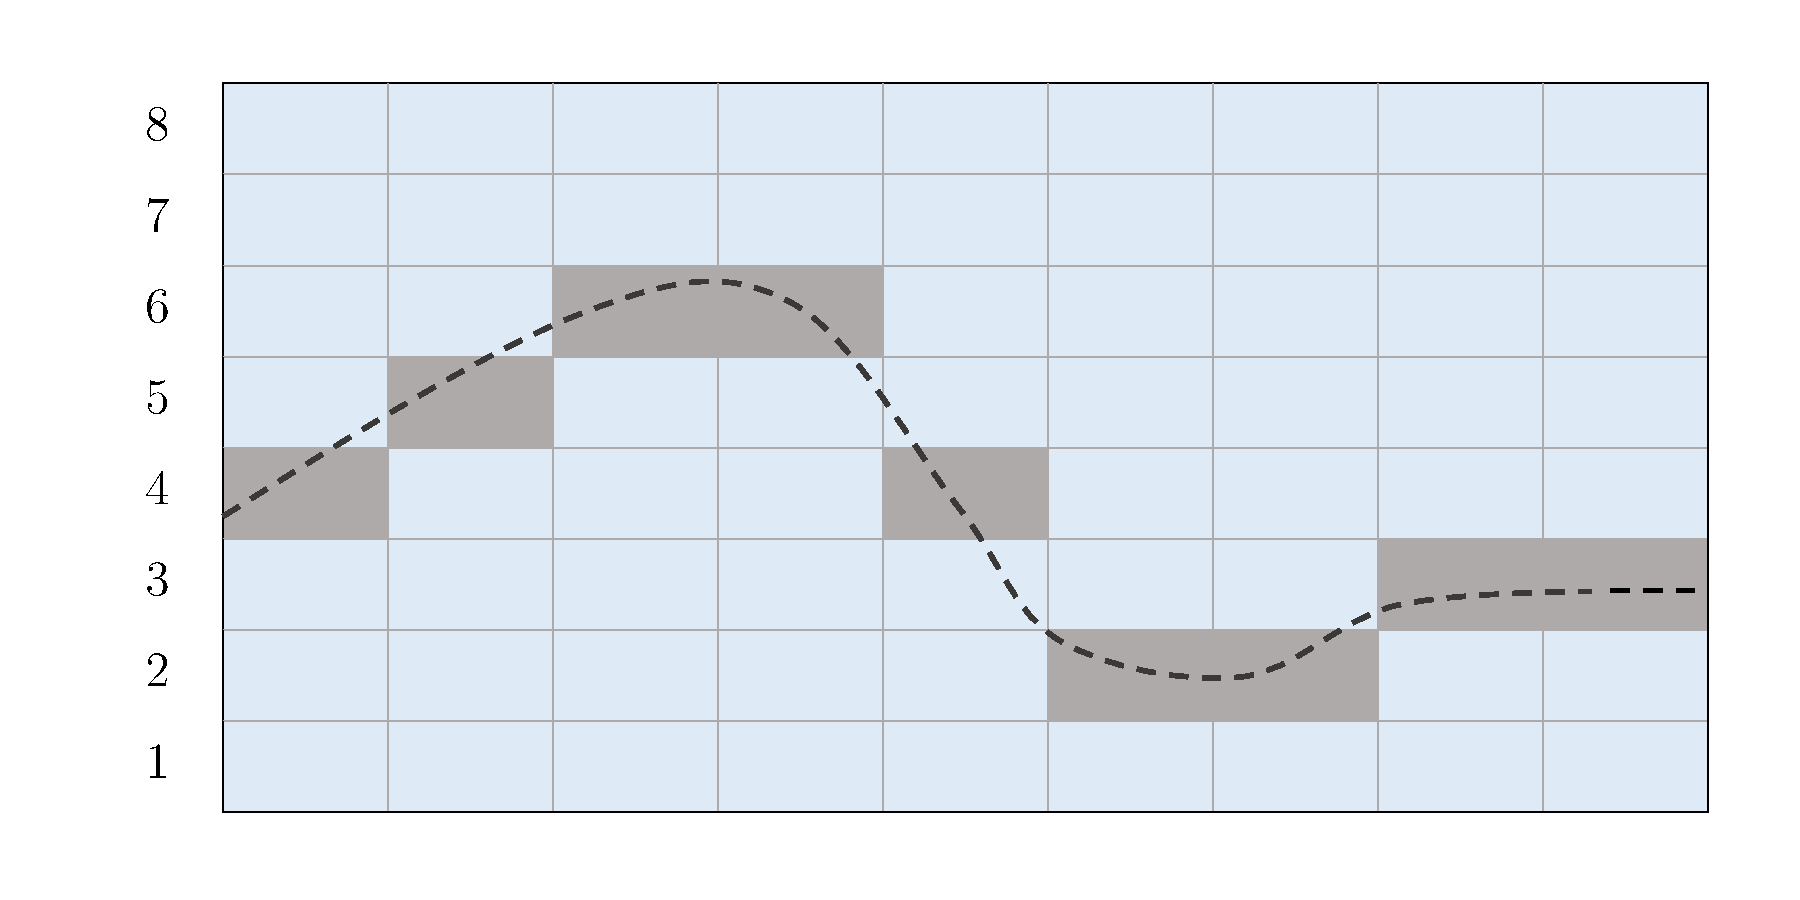
\includegraphics[scale=0.4]{figures/quantization.pdf}
    \caption[Example of a quantized contour]{Example of a quantized contour. The \ac{F0} contour is represented by a dashed line. The darker rectangles represent the corresponding quantized contour.}
    \label{fig:quantization}
\end{figure}

From the perspective of learning, quantization has the effect of converting \ac{F0} modeling from a regression problem to a classification one.
More specifically, under a quantized regime, a \ac{DNN} would not attempt to approximate an underlying function of the contours, but rather a function of the probabilities of the categorical symbols from which the observed contour is generated.

This decision might seem rather odd at first, as most researchers usually choose to preserve the original continuous \ac{F0} values and try to model the underlying function of the contour.
I decided against this approach because in my estimation it might restrict and flatten the possible contours that the model can output.
This is due to the fact that, as the model tries to reconstruct the underlying function, it will interpolate and smooth it to fit the training data.
This has the effect of producing an averaged-out version of the observation.

In order to avoid this, I decided not to use numerical values and to replace them with categorical data describing quantized pitch jumps.
As the categorical data represents clear pre-defined pitch movements and not static values, pitch values are not forced to fit into a smoothed function of the contour, but rather a function of the probabilities of the categorical symbols from which the static \ac{F0} contours are generated.
This means that the model is less restricted with regard to how fast pitch values can change or how far up or down they can jump, because the weights of the network are not modeling the actual size of the output values, but rather probabilities of pre-defined pitch movements.

The inclusion of quantization as a feature is also justified by the fact that \ac{F0} is limited to a specific frequency range (typically 85 to 180~Hz for males and 165 to 255~Hz for females) and that very small pitch variations (say, 100 and 100.02~Hz) are not that important in the context of \ac{TTS}, where reconstructed \ac{F0} contours often only approximate the original.
This is for instance the main assumption underlying the IPO intonation model (see \autoref{sec:intonation-models} for more details), where contours are simplified to only preserve perceptually relevant prosodic features and where less important features such as micro-prosody are discarded.

In my encoding scheme, quantization is achieved by the recursive application of \autoref{eq:frequency-equation}, which automatically maps the static \ac{F0} values to a quantized frequency space (i.e., a pitch scale).
This equation is more commonly used to determine the frequency of notes of the equal-tempered western scale, i.e., a scale where each octave is divided into (twelve) equally-sized steps.
In my implementation, the use of this formula was slightly different from its more common application, as it not used to directly partition the frequency space into levels, but rather to estimate the number of pitch levels separating one observed \ac{F0} and next.

The choice of basing the encoding scheme on this particular scale is somewhat unconventional, as a more common choice in speech applications would be to utilize a mel scale.
One reason behind this decision is the criticism surrounding the mel scale put forward by Donald D. Greenwood, a student of Stevens who worked on the mel scale experiments in 1956, who considers the scale to be biased by experimental flaws \citep{Greenwood1997Mel}.
\autoref{eq:frequency-equation}, on the other hand, is purely based on well-understood physics of sound, as it was not determined empirically through the judgment of test subjects.

Secondly, \autoref{eq:frequency-equation} is adopted for the sake of convenience, as it much easier to debug and check the sanity of the encoding when the encoded values have a clearly interpretable meaning.
For instance, if we set $s$ to $24$, each interval in the scale corresponds exactly to half a semitone of the standard western scale.

The idea of quantizing contours is not new in the context of \ac{F0} modeling. 
In a recent proposal, quantization of \ac{F0} into static discrete values has been adopted as a way of avoiding \ac{F0} interpolation \citep{Wang2017RNN}.
In particular, unspecified \ac{F0} values (e.g., in the presence of unvoiced segments) are encoded by a dedicated categorical symbol.
This is argued to help avoid the influence of prosodic artifacts created during the interpolation process.
From the perspective of dynamism, this approach is functionally very similar to calculating the log of \ac{F0} values: quantization simply linearizes the logarithmic relationship between \ac{F0} and pitch, with the difference that the static representations are discrete.

However, in the methodology proposed here, quantization carries out a completely different function, as it is not used to avoid interpolation, but rather to provide a quantized space as the basis for the calculation of the dynamics.
In the proposed approach, it is not possible to do away with interpolation, because each \ac{F0} label is defined in relation to the previous one, which means we can never leave the value of \ac{F0} unspecified, otherwise all the following \ac{F0} labels would become uninterpretable. 
Therefore, here, quantization of the frequency domain is just an indirect way of ensuring that dynamics are also quantized and not real-valued.



\subsection{Static vs.\ Dynamic}

The main feature of the proposed encoding is its dynamism.
This means that contours are not encoded as a sequence of static values, but rather as a sequence of values representing the dynamic evolution of the contour through time.

This idea stems from a number of empirical and anecdotal observations that can be made about pitch both in the context of speech and music.
In particular, the first observation is that raw \ac{F0} measurements assign an absolute value to each sample, and this value is completely meaningless when taken in isolation.
It is only when \ac{F0} values are presented in context that they are endowed with prosodic meaning.

This closely mirrors a similar observation that can be made about the musical domain.
In music, notes, just like speech pitch points, are completely meaningless by themselves.
As most musicians will know, what in fact constitutes a melody is not so much the sequence of notes, but the sequence of musical intervals, i.e., the relative change between one note and the next one. 
This is especially apparent if we consider that most people who can sing a tune can do so without any knowledge about the name of the notes in the melody. 
Melodies are also routinely transposed (i.e., pitch translation) to suit various voice ranges without changing the musical message of the tune.
All this can be explained by the fact that, to a large extent, humans, with the possible exception of those born with perfect pitch, do not rely on absolute measurements to produce and process musical pitch.
 
Similarly to what happens in music, humans do not know the exact \ac{F0} values they process or produce (again with the exception of those with perfect pitch) and yet, they are still able to correctly generate and interpret intonation patterns.
Furthermore, speech patterns can also be transposed, i.e., when for instance they are uttered by people with different voice registers, without much change in the prosodic message (e.g., a question is interpreted as a question regardless of the shift of the contour along the frequency axis).

We do not wish to take this analogy any further.
Speech and music are after all two completely different domains and there is even some evidence that the processing of pitch information differs significantly for speech and music phenomena.
\citet{Zatorre2012Musical} suggest that there are two pitch-related processing systems in the human brain: one for coarse and approximate pitch analysis, and one for precise and fine-grained analysis.
Of these, it is suggested that the latter is unique to music.
Because of the significant differences between the two domains, within the scope of the present discussion, the only loose analogy that we wish to take advantage of is the fact that the encoding of both musical or prosodic messages relies on a somewhat more relative dimension of frequency than an absolute one.

The importance of a dynamic representation of the contour rests in its ability to capture a more abstract and compact representation, endowed with a higher degree of invariance.
This property is illustrated by \autoref{fig:translation}.
As it can be observed, the static values after the upward translation are completely different.
On the other hand, a dynamic representation is completely invariant to frequency translation:

\begin{figure}[H]
    \centering
    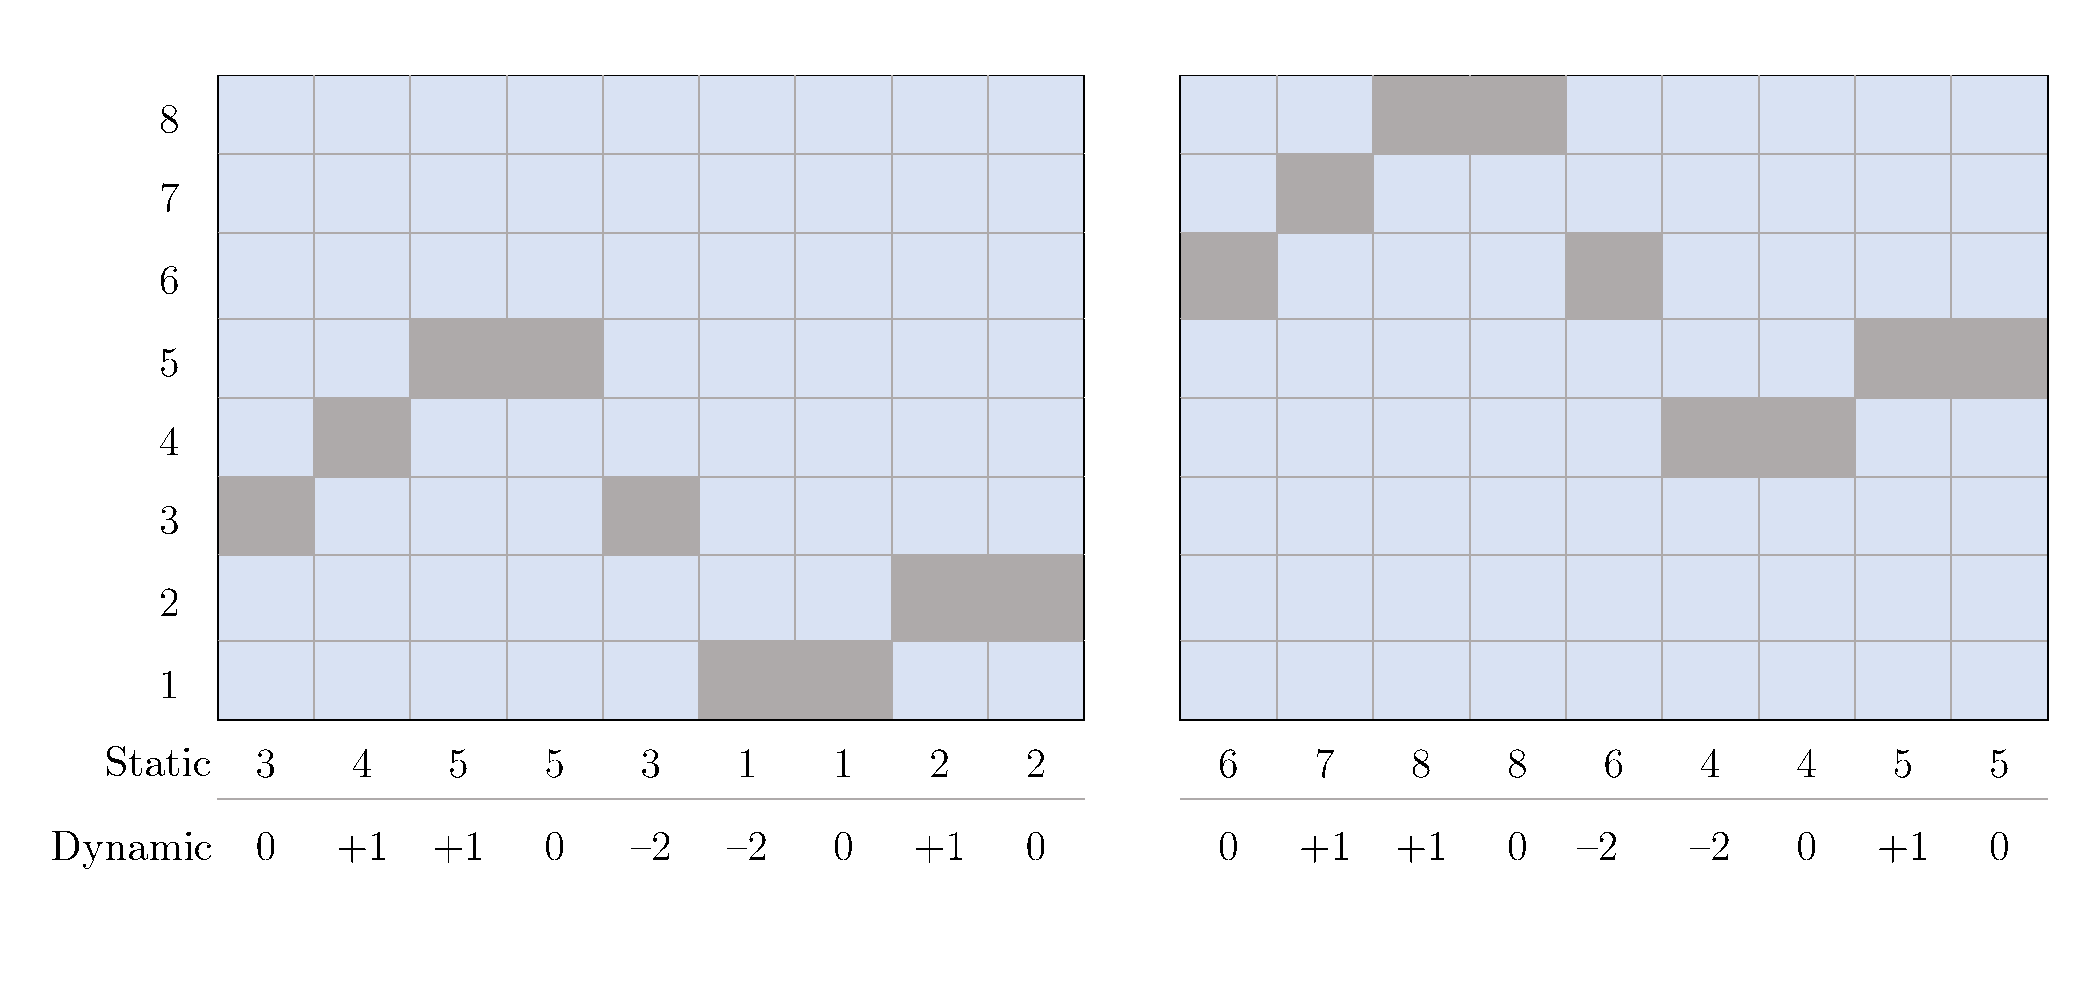
\includegraphics[scale=0.38]{figures/translation.pdf}
    \caption[Contour translation]{On the left side of the figure, a quantized \ac{F0} contour is shown. On the right side, the same quantized \ac{F0} contour has been shifted upwards by three steps. At the bottom of the figure, the corresponding static and dynamic values are reported.}
    \label{fig:translation}
\end{figure}

As a side effect, the proposed encoding scheme is also naturally register-independent, as any upward or downward translation of the original contour would yield the same encoded sequence.
This means it can be used to seamlessly model intonation of multi-speaker corpora without any additional normalization steps.


\subsection{Sign Separation}

One important feature of the proposed encoding scheme is the decomposition of pitch intervals into sign and magnitude information.
The reason for the separation of these two types of information is justified first and foremost as a way of reducing the number of possible outcomes by half.

One additional advantage of this separation is that we are also able to produce a representation that has a higher degree of invariance to compression and dilation, especially with regard to sign information.
This property is illustrated by \autoref{fig:dilation}, where we can see how the sign of a contour remains unaltered, even after dilation has taken place.
We can also observe that the magnitude, similarly to traditional static values, is more susceptible to noise.



\begin{figure}[H]
    \centering
    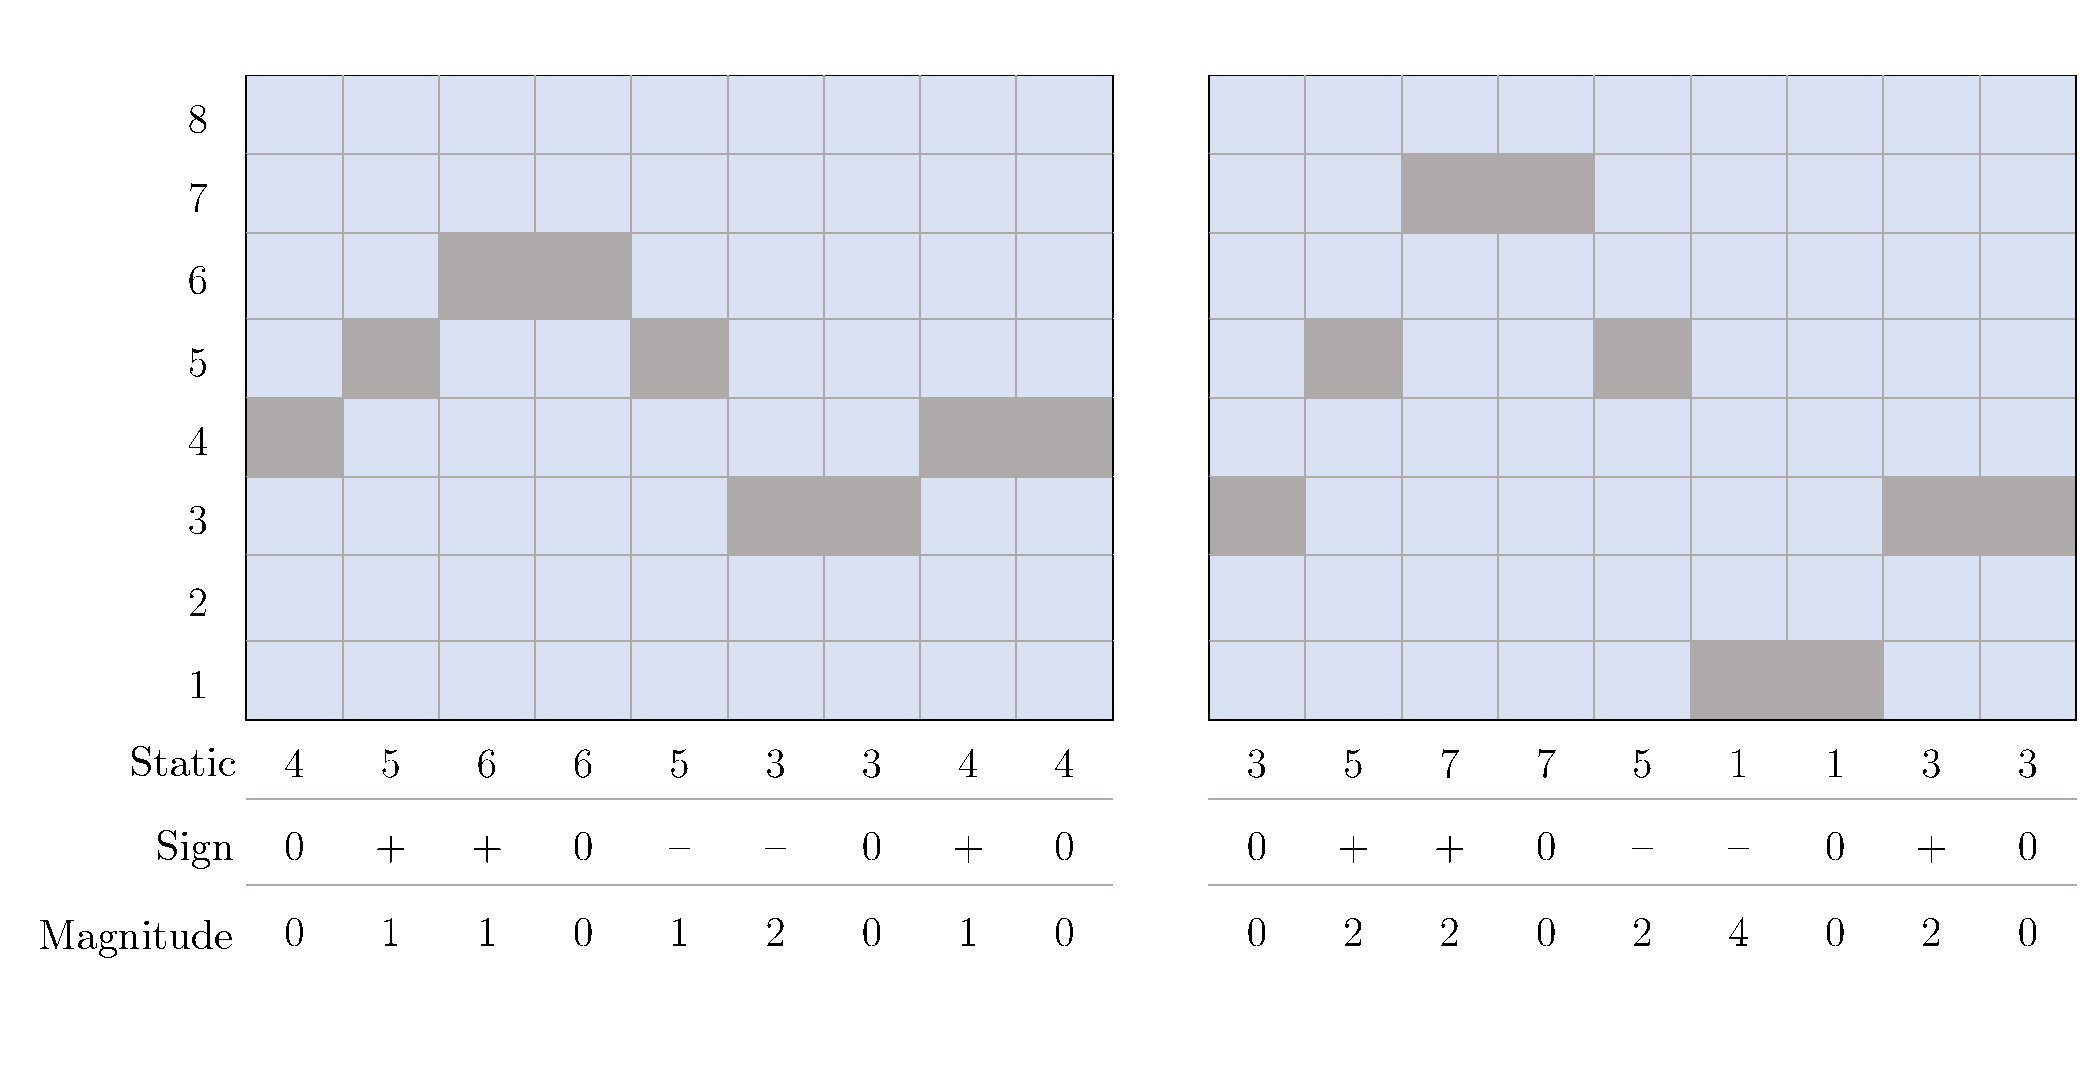
\includegraphics[scale=0.35]{figures/dilation.pdf}
    \caption[Contour dilation]{On the left side of the figure, a quantized \ac{F0} contour is shown. On the right side, the same quantized \ac{F0} contour has undergone dilation. At the bottom of the figure, the corresponding static and dynamic values are reported. The dynamic values are represented by the corresponding sign and magnitude values.}
    \label{fig:dilation}
\end{figure}




\subsection{Magnitude Compression}

The last main feature that characterizes the proposed dynamic approach is its compressing effect.
Compression is achieved in a first instance by means of quantization, as this greatly restricts the possible number of outcomes.
This is because the continuous infinite space is mapped to simplified quantized space with a discrete and finite number of possible output values.

A second source of compression is provided by the separation of sign and magnitude information.
This atomizes the contour representation into its minimal components: the direction of movement and the amount thereof.

Even though separating the sign and the magnitude reduces the number of possible outcomes by half, the number of magnitude labels is still much too great and wasteful if not properly compressed.
This is especially true as far as large intervals are concerned, where we might not want to model the small difference between extremely large interval values.

One way to reduce the number of labels, would be to use larger steps by setting the $s$ parameter in \autoref{eq:frequency-equation} to a lower value.
This, however, would also reduce our ability to encode smaller prosodic movements, which would result in very imprecise contour reconstruction.
Ideally, our encoding scheme should be able to model most prosodic events, so both small and large intervals.

However, we might not wish to model them with the same level of precision, since small differences between large intervals might be less important to model.
If the processing of pitch information for speech is based on a fairly coarse-grained analysis of pitch as suggested in \citep{Zatorre2012Musical}, encoding fine-grained differences is unnecessary.

For these reasons, a third source of compression is added.
In the proposed encoding, the number of possible magnitude values is drastically reduced by rounding magnitude values to their closest triangular number approximation.
Triangular numbers are a sequence of numbers that are obtained by continued summation of natural numbers.

For instance, the sequence of natural numbers ``$1, 2, 3, 4, 5$, etc.'' would yield the sequence of triangular numbers ``$1, 3, 6, 10, 15$, etc.''.
For my encoding scheme, an additional 0\textsuperscript{th} triangular number is included, i.e., ``$0, 1, 3, 6, 10, 15$, etc.''.

Triangular numbers have the nice property that the distance between each number and the next one grows linearly.
When we only consider intervals whose index is a triangular number we are able to consider intervals with a linearly decreasing precision.
This means that we are able to model small intervals very precisely, with the trade-off that we model large intervals less precisely.



\subsection{Encoded Contours}

In order to assess the validity and usefulness of my encoding, I compared the original contours with their encoded-decoded counterparts by plotting and listening to their copy-synthesis.


\autoref{fig:reconstructed} shows an original contour along with its encoded and decoded counterpart. 
As we can see, the original and the reconstructed contours are quite similar, albeit with a few subtle differences. 
In particular, observe in \autoref{fig:reconstructed} how all the numbers of steps in each pitch interval are triangular numbers (i.e., $0, 1, 3, 6, 10, 15$, etc.).
For instance, the second syllable (i.e., ``mid'') has two intervals, where the first one has 10 steps and the second one, 6.
Also, notice how the reconstructed contour occasionally overshoots or undershoots.
For example, in the fifth syllable (i.e., ``naits''), the first pitch interval contains only 3 steps instead of the more accurate 4.

\begin{figure}[h]
\centering
\resizebox{\textwidth}{!}{%% Creator: Matplotlib, PGF backend
%%
%% To include the figure in your LaTeX document, write
%%   \input{<filename>.pgf}
%%
%% Make sure the required packages are loaded in your preamble
%%   \usepackage{pgf}
%%
%% Figures using additional raster images can only be included by \input if
%% they are in the same directory as the main LaTeX file. For loading figures
%% from other directories you can use the `import` package
%%   \usepackage{import}
%% and then include the figures with
%%   \import{<path to file>}{<filename>.pgf}
%%
%% Matplotlib used the following preamble
%%   \usepackage[utf8x]{inputenc}
%%   \usepackage[T1]{fontenc}
%%   \usepackage{cmbright}
%%
\begingroup%
\makeatletter%
\begin{pgfpicture}%
\pgfpathrectangle{\pgfpointorigin}{\pgfqpoint{8.000000in}{5.000000in}}%
\pgfusepath{use as bounding box, clip}%
\begin{pgfscope}%
\pgfsetbuttcap%
\pgfsetmiterjoin%
\definecolor{currentfill}{rgb}{1.000000,1.000000,1.000000}%
\pgfsetfillcolor{currentfill}%
\pgfsetlinewidth{0.000000pt}%
\definecolor{currentstroke}{rgb}{1.000000,1.000000,1.000000}%
\pgfsetstrokecolor{currentstroke}%
\pgfsetdash{}{0pt}%
\pgfpathmoveto{\pgfqpoint{0.000000in}{0.000000in}}%
\pgfpathlineto{\pgfqpoint{8.000000in}{0.000000in}}%
\pgfpathlineto{\pgfqpoint{8.000000in}{5.000000in}}%
\pgfpathlineto{\pgfqpoint{0.000000in}{5.000000in}}%
\pgfpathclose%
\pgfusepath{fill}%
\end{pgfscope}%
\begin{pgfscope}%
\pgfsetbuttcap%
\pgfsetmiterjoin%
\definecolor{currentfill}{rgb}{1.000000,1.000000,1.000000}%
\pgfsetfillcolor{currentfill}%
\pgfsetlinewidth{0.000000pt}%
\definecolor{currentstroke}{rgb}{0.000000,0.000000,0.000000}%
\pgfsetstrokecolor{currentstroke}%
\pgfsetstrokeopacity{0.000000}%
\pgfsetdash{}{0pt}%
\pgfpathmoveto{\pgfqpoint{1.000000in}{0.550000in}}%
\pgfpathlineto{\pgfqpoint{7.200000in}{0.550000in}}%
\pgfpathlineto{\pgfqpoint{7.200000in}{4.400000in}}%
\pgfpathlineto{\pgfqpoint{1.000000in}{4.400000in}}%
\pgfpathclose%
\pgfusepath{fill}%
\end{pgfscope}%
\begin{pgfscope}%
\pgfsetbuttcap%
\pgfsetroundjoin%
\definecolor{currentfill}{rgb}{0.000000,0.000000,0.000000}%
\pgfsetfillcolor{currentfill}%
\pgfsetlinewidth{0.803000pt}%
\definecolor{currentstroke}{rgb}{0.000000,0.000000,0.000000}%
\pgfsetstrokecolor{currentstroke}%
\pgfsetdash{}{0pt}%
\pgfsys@defobject{currentmarker}{\pgfqpoint{0.000000in}{-0.048611in}}{\pgfqpoint{0.000000in}{0.000000in}}{%
\pgfpathmoveto{\pgfqpoint{0.000000in}{0.000000in}}%
\pgfpathlineto{\pgfqpoint{0.000000in}{-0.048611in}}%
\pgfusepath{stroke,fill}%
}%
\begin{pgfscope}%
\pgfsys@transformshift{1.281818in}{0.550000in}%
\pgfsys@useobject{currentmarker}{}%
\end{pgfscope}%
\end{pgfscope}%
\begin{pgfscope}%
\pgftext[x=1.281818in,y=0.452778in,,top]{\rmfamily\fontsize{10.000000}{12.000000}\selectfont \(\displaystyle 0.00\)}%
\end{pgfscope}%
\begin{pgfscope}%
\pgfsetbuttcap%
\pgfsetroundjoin%
\definecolor{currentfill}{rgb}{0.000000,0.000000,0.000000}%
\pgfsetfillcolor{currentfill}%
\pgfsetlinewidth{0.803000pt}%
\definecolor{currentstroke}{rgb}{0.000000,0.000000,0.000000}%
\pgfsetstrokecolor{currentstroke}%
\pgfsetdash{}{0pt}%
\pgfsys@defobject{currentmarker}{\pgfqpoint{0.000000in}{-0.048611in}}{\pgfqpoint{0.000000in}{0.000000in}}{%
\pgfpathmoveto{\pgfqpoint{0.000000in}{0.000000in}}%
\pgfpathlineto{\pgfqpoint{0.000000in}{-0.048611in}}%
\pgfusepath{stroke,fill}%
}%
\begin{pgfscope}%
\pgfsys@transformshift{2.043489in}{0.550000in}%
\pgfsys@useobject{currentmarker}{}%
\end{pgfscope}%
\end{pgfscope}%
\begin{pgfscope}%
\pgftext[x=2.043489in,y=0.452778in,,top]{\rmfamily\fontsize{10.000000}{12.000000}\selectfont \(\displaystyle 0.25\)}%
\end{pgfscope}%
\begin{pgfscope}%
\pgfsetbuttcap%
\pgfsetroundjoin%
\definecolor{currentfill}{rgb}{0.000000,0.000000,0.000000}%
\pgfsetfillcolor{currentfill}%
\pgfsetlinewidth{0.803000pt}%
\definecolor{currentstroke}{rgb}{0.000000,0.000000,0.000000}%
\pgfsetstrokecolor{currentstroke}%
\pgfsetdash{}{0pt}%
\pgfsys@defobject{currentmarker}{\pgfqpoint{0.000000in}{-0.048611in}}{\pgfqpoint{0.000000in}{0.000000in}}{%
\pgfpathmoveto{\pgfqpoint{0.000000in}{0.000000in}}%
\pgfpathlineto{\pgfqpoint{0.000000in}{-0.048611in}}%
\pgfusepath{stroke,fill}%
}%
\begin{pgfscope}%
\pgfsys@transformshift{2.805160in}{0.550000in}%
\pgfsys@useobject{currentmarker}{}%
\end{pgfscope}%
\end{pgfscope}%
\begin{pgfscope}%
\pgftext[x=2.805160in,y=0.452778in,,top]{\rmfamily\fontsize{10.000000}{12.000000}\selectfont \(\displaystyle 0.50\)}%
\end{pgfscope}%
\begin{pgfscope}%
\pgfsetbuttcap%
\pgfsetroundjoin%
\definecolor{currentfill}{rgb}{0.000000,0.000000,0.000000}%
\pgfsetfillcolor{currentfill}%
\pgfsetlinewidth{0.803000pt}%
\definecolor{currentstroke}{rgb}{0.000000,0.000000,0.000000}%
\pgfsetstrokecolor{currentstroke}%
\pgfsetdash{}{0pt}%
\pgfsys@defobject{currentmarker}{\pgfqpoint{0.000000in}{-0.048611in}}{\pgfqpoint{0.000000in}{0.000000in}}{%
\pgfpathmoveto{\pgfqpoint{0.000000in}{0.000000in}}%
\pgfpathlineto{\pgfqpoint{0.000000in}{-0.048611in}}%
\pgfusepath{stroke,fill}%
}%
\begin{pgfscope}%
\pgfsys@transformshift{3.566830in}{0.550000in}%
\pgfsys@useobject{currentmarker}{}%
\end{pgfscope}%
\end{pgfscope}%
\begin{pgfscope}%
\pgftext[x=3.566830in,y=0.452778in,,top]{\rmfamily\fontsize{10.000000}{12.000000}\selectfont \(\displaystyle 0.75\)}%
\end{pgfscope}%
\begin{pgfscope}%
\pgfsetbuttcap%
\pgfsetroundjoin%
\definecolor{currentfill}{rgb}{0.000000,0.000000,0.000000}%
\pgfsetfillcolor{currentfill}%
\pgfsetlinewidth{0.803000pt}%
\definecolor{currentstroke}{rgb}{0.000000,0.000000,0.000000}%
\pgfsetstrokecolor{currentstroke}%
\pgfsetdash{}{0pt}%
\pgfsys@defobject{currentmarker}{\pgfqpoint{0.000000in}{-0.048611in}}{\pgfqpoint{0.000000in}{0.000000in}}{%
\pgfpathmoveto{\pgfqpoint{0.000000in}{0.000000in}}%
\pgfpathlineto{\pgfqpoint{0.000000in}{-0.048611in}}%
\pgfusepath{stroke,fill}%
}%
\begin{pgfscope}%
\pgfsys@transformshift{4.328501in}{0.550000in}%
\pgfsys@useobject{currentmarker}{}%
\end{pgfscope}%
\end{pgfscope}%
\begin{pgfscope}%
\pgftext[x=4.328501in,y=0.452778in,,top]{\rmfamily\fontsize{10.000000}{12.000000}\selectfont \(\displaystyle 1.00\)}%
\end{pgfscope}%
\begin{pgfscope}%
\pgfsetbuttcap%
\pgfsetroundjoin%
\definecolor{currentfill}{rgb}{0.000000,0.000000,0.000000}%
\pgfsetfillcolor{currentfill}%
\pgfsetlinewidth{0.803000pt}%
\definecolor{currentstroke}{rgb}{0.000000,0.000000,0.000000}%
\pgfsetstrokecolor{currentstroke}%
\pgfsetdash{}{0pt}%
\pgfsys@defobject{currentmarker}{\pgfqpoint{0.000000in}{-0.048611in}}{\pgfqpoint{0.000000in}{0.000000in}}{%
\pgfpathmoveto{\pgfqpoint{0.000000in}{0.000000in}}%
\pgfpathlineto{\pgfqpoint{0.000000in}{-0.048611in}}%
\pgfusepath{stroke,fill}%
}%
\begin{pgfscope}%
\pgfsys@transformshift{5.090172in}{0.550000in}%
\pgfsys@useobject{currentmarker}{}%
\end{pgfscope}%
\end{pgfscope}%
\begin{pgfscope}%
\pgftext[x=5.090172in,y=0.452778in,,top]{\rmfamily\fontsize{10.000000}{12.000000}\selectfont \(\displaystyle 1.25\)}%
\end{pgfscope}%
\begin{pgfscope}%
\pgfsetbuttcap%
\pgfsetroundjoin%
\definecolor{currentfill}{rgb}{0.000000,0.000000,0.000000}%
\pgfsetfillcolor{currentfill}%
\pgfsetlinewidth{0.803000pt}%
\definecolor{currentstroke}{rgb}{0.000000,0.000000,0.000000}%
\pgfsetstrokecolor{currentstroke}%
\pgfsetdash{}{0pt}%
\pgfsys@defobject{currentmarker}{\pgfqpoint{0.000000in}{-0.048611in}}{\pgfqpoint{0.000000in}{0.000000in}}{%
\pgfpathmoveto{\pgfqpoint{0.000000in}{0.000000in}}%
\pgfpathlineto{\pgfqpoint{0.000000in}{-0.048611in}}%
\pgfusepath{stroke,fill}%
}%
\begin{pgfscope}%
\pgfsys@transformshift{5.851843in}{0.550000in}%
\pgfsys@useobject{currentmarker}{}%
\end{pgfscope}%
\end{pgfscope}%
\begin{pgfscope}%
\pgftext[x=5.851843in,y=0.452778in,,top]{\rmfamily\fontsize{10.000000}{12.000000}\selectfont \(\displaystyle 1.50\)}%
\end{pgfscope}%
\begin{pgfscope}%
\pgfsetbuttcap%
\pgfsetroundjoin%
\definecolor{currentfill}{rgb}{0.000000,0.000000,0.000000}%
\pgfsetfillcolor{currentfill}%
\pgfsetlinewidth{0.803000pt}%
\definecolor{currentstroke}{rgb}{0.000000,0.000000,0.000000}%
\pgfsetstrokecolor{currentstroke}%
\pgfsetdash{}{0pt}%
\pgfsys@defobject{currentmarker}{\pgfqpoint{0.000000in}{-0.048611in}}{\pgfqpoint{0.000000in}{0.000000in}}{%
\pgfpathmoveto{\pgfqpoint{0.000000in}{0.000000in}}%
\pgfpathlineto{\pgfqpoint{0.000000in}{-0.048611in}}%
\pgfusepath{stroke,fill}%
}%
\begin{pgfscope}%
\pgfsys@transformshift{6.613514in}{0.550000in}%
\pgfsys@useobject{currentmarker}{}%
\end{pgfscope}%
\end{pgfscope}%
\begin{pgfscope}%
\pgftext[x=6.613514in,y=0.452778in,,top]{\rmfamily\fontsize{10.000000}{12.000000}\selectfont \(\displaystyle 1.75\)}%
\end{pgfscope}%
\begin{pgfscope}%
\pgftext[x=4.100000in,y=0.274567in,,top]{\rmfamily\fontsize{10.000000}{12.000000}\selectfont Time (s)}%
\end{pgfscope}%
\begin{pgfscope}%
\pgfsetbuttcap%
\pgfsetroundjoin%
\definecolor{currentfill}{rgb}{0.000000,0.000000,0.000000}%
\pgfsetfillcolor{currentfill}%
\pgfsetlinewidth{0.803000pt}%
\definecolor{currentstroke}{rgb}{0.000000,0.000000,0.000000}%
\pgfsetstrokecolor{currentstroke}%
\pgfsetdash{}{0pt}%
\pgfsys@defobject{currentmarker}{\pgfqpoint{-0.048611in}{0.000000in}}{\pgfqpoint{0.000000in}{0.000000in}}{%
\pgfpathmoveto{\pgfqpoint{0.000000in}{0.000000in}}%
\pgfpathlineto{\pgfqpoint{-0.048611in}{0.000000in}}%
\pgfusepath{stroke,fill}%
}%
\begin{pgfscope}%
\pgfsys@transformshift{1.000000in}{0.934202in}%
\pgfsys@useobject{currentmarker}{}%
\end{pgfscope}%
\end{pgfscope}%
\begin{pgfscope}%
\pgftext[x=0.684030in,y=0.886375in,left,base]{\rmfamily\fontsize{10.000000}{12.000000}\selectfont \(\displaystyle 140\)}%
\end{pgfscope}%
\begin{pgfscope}%
\pgfsetbuttcap%
\pgfsetroundjoin%
\definecolor{currentfill}{rgb}{0.000000,0.000000,0.000000}%
\pgfsetfillcolor{currentfill}%
\pgfsetlinewidth{0.803000pt}%
\definecolor{currentstroke}{rgb}{0.000000,0.000000,0.000000}%
\pgfsetstrokecolor{currentstroke}%
\pgfsetdash{}{0pt}%
\pgfsys@defobject{currentmarker}{\pgfqpoint{-0.048611in}{0.000000in}}{\pgfqpoint{0.000000in}{0.000000in}}{%
\pgfpathmoveto{\pgfqpoint{0.000000in}{0.000000in}}%
\pgfpathlineto{\pgfqpoint{-0.048611in}{0.000000in}}%
\pgfusepath{stroke,fill}%
}%
\begin{pgfscope}%
\pgfsys@transformshift{1.000000in}{1.467119in}%
\pgfsys@useobject{currentmarker}{}%
\end{pgfscope}%
\end{pgfscope}%
\begin{pgfscope}%
\pgftext[x=0.684030in,y=1.419291in,left,base]{\rmfamily\fontsize{10.000000}{12.000000}\selectfont \(\displaystyle 160\)}%
\end{pgfscope}%
\begin{pgfscope}%
\pgfsetbuttcap%
\pgfsetroundjoin%
\definecolor{currentfill}{rgb}{0.000000,0.000000,0.000000}%
\pgfsetfillcolor{currentfill}%
\pgfsetlinewidth{0.803000pt}%
\definecolor{currentstroke}{rgb}{0.000000,0.000000,0.000000}%
\pgfsetstrokecolor{currentstroke}%
\pgfsetdash{}{0pt}%
\pgfsys@defobject{currentmarker}{\pgfqpoint{-0.048611in}{0.000000in}}{\pgfqpoint{0.000000in}{0.000000in}}{%
\pgfpathmoveto{\pgfqpoint{0.000000in}{0.000000in}}%
\pgfpathlineto{\pgfqpoint{-0.048611in}{0.000000in}}%
\pgfusepath{stroke,fill}%
}%
\begin{pgfscope}%
\pgfsys@transformshift{1.000000in}{2.000036in}%
\pgfsys@useobject{currentmarker}{}%
\end{pgfscope}%
\end{pgfscope}%
\begin{pgfscope}%
\pgftext[x=0.684030in,y=1.952208in,left,base]{\rmfamily\fontsize{10.000000}{12.000000}\selectfont \(\displaystyle 180\)}%
\end{pgfscope}%
\begin{pgfscope}%
\pgfsetbuttcap%
\pgfsetroundjoin%
\definecolor{currentfill}{rgb}{0.000000,0.000000,0.000000}%
\pgfsetfillcolor{currentfill}%
\pgfsetlinewidth{0.803000pt}%
\definecolor{currentstroke}{rgb}{0.000000,0.000000,0.000000}%
\pgfsetstrokecolor{currentstroke}%
\pgfsetdash{}{0pt}%
\pgfsys@defobject{currentmarker}{\pgfqpoint{-0.048611in}{0.000000in}}{\pgfqpoint{0.000000in}{0.000000in}}{%
\pgfpathmoveto{\pgfqpoint{0.000000in}{0.000000in}}%
\pgfpathlineto{\pgfqpoint{-0.048611in}{0.000000in}}%
\pgfusepath{stroke,fill}%
}%
\begin{pgfscope}%
\pgfsys@transformshift{1.000000in}{2.532953in}%
\pgfsys@useobject{currentmarker}{}%
\end{pgfscope}%
\end{pgfscope}%
\begin{pgfscope}%
\pgftext[x=0.684030in,y=2.485125in,left,base]{\rmfamily\fontsize{10.000000}{12.000000}\selectfont \(\displaystyle 200\)}%
\end{pgfscope}%
\begin{pgfscope}%
\pgfsetbuttcap%
\pgfsetroundjoin%
\definecolor{currentfill}{rgb}{0.000000,0.000000,0.000000}%
\pgfsetfillcolor{currentfill}%
\pgfsetlinewidth{0.803000pt}%
\definecolor{currentstroke}{rgb}{0.000000,0.000000,0.000000}%
\pgfsetstrokecolor{currentstroke}%
\pgfsetdash{}{0pt}%
\pgfsys@defobject{currentmarker}{\pgfqpoint{-0.048611in}{0.000000in}}{\pgfqpoint{0.000000in}{0.000000in}}{%
\pgfpathmoveto{\pgfqpoint{0.000000in}{0.000000in}}%
\pgfpathlineto{\pgfqpoint{-0.048611in}{0.000000in}}%
\pgfusepath{stroke,fill}%
}%
\begin{pgfscope}%
\pgfsys@transformshift{1.000000in}{3.065869in}%
\pgfsys@useobject{currentmarker}{}%
\end{pgfscope}%
\end{pgfscope}%
\begin{pgfscope}%
\pgftext[x=0.684030in,y=3.018042in,left,base]{\rmfamily\fontsize{10.000000}{12.000000}\selectfont \(\displaystyle 220\)}%
\end{pgfscope}%
\begin{pgfscope}%
\pgfsetbuttcap%
\pgfsetroundjoin%
\definecolor{currentfill}{rgb}{0.000000,0.000000,0.000000}%
\pgfsetfillcolor{currentfill}%
\pgfsetlinewidth{0.803000pt}%
\definecolor{currentstroke}{rgb}{0.000000,0.000000,0.000000}%
\pgfsetstrokecolor{currentstroke}%
\pgfsetdash{}{0pt}%
\pgfsys@defobject{currentmarker}{\pgfqpoint{-0.048611in}{0.000000in}}{\pgfqpoint{0.000000in}{0.000000in}}{%
\pgfpathmoveto{\pgfqpoint{0.000000in}{0.000000in}}%
\pgfpathlineto{\pgfqpoint{-0.048611in}{0.000000in}}%
\pgfusepath{stroke,fill}%
}%
\begin{pgfscope}%
\pgfsys@transformshift{1.000000in}{3.598786in}%
\pgfsys@useobject{currentmarker}{}%
\end{pgfscope}%
\end{pgfscope}%
\begin{pgfscope}%
\pgftext[x=0.684030in,y=3.550958in,left,base]{\rmfamily\fontsize{10.000000}{12.000000}\selectfont \(\displaystyle 240\)}%
\end{pgfscope}%
\begin{pgfscope}%
\pgfsetbuttcap%
\pgfsetroundjoin%
\definecolor{currentfill}{rgb}{0.000000,0.000000,0.000000}%
\pgfsetfillcolor{currentfill}%
\pgfsetlinewidth{0.803000pt}%
\definecolor{currentstroke}{rgb}{0.000000,0.000000,0.000000}%
\pgfsetstrokecolor{currentstroke}%
\pgfsetdash{}{0pt}%
\pgfsys@defobject{currentmarker}{\pgfqpoint{-0.048611in}{0.000000in}}{\pgfqpoint{0.000000in}{0.000000in}}{%
\pgfpathmoveto{\pgfqpoint{0.000000in}{0.000000in}}%
\pgfpathlineto{\pgfqpoint{-0.048611in}{0.000000in}}%
\pgfusepath{stroke,fill}%
}%
\begin{pgfscope}%
\pgfsys@transformshift{1.000000in}{4.131703in}%
\pgfsys@useobject{currentmarker}{}%
\end{pgfscope}%
\end{pgfscope}%
\begin{pgfscope}%
\pgftext[x=0.684030in,y=4.083875in,left,base]{\rmfamily\fontsize{10.000000}{12.000000}\selectfont \(\displaystyle 260\)}%
\end{pgfscope}%
\begin{pgfscope}%
\pgftext[x=0.628474in,y=2.475000in,,bottom,rotate=90.000000]{\rmfamily\fontsize{10.000000}{12.000000}\selectfont Frequency (Hz)}%
\end{pgfscope}%
\begin{pgfscope}%
\pgfpathrectangle{\pgfqpoint{1.000000in}{0.550000in}}{\pgfqpoint{6.200000in}{3.850000in}} %
\pgfusepath{clip}%
\pgfsetrectcap%
\pgfsetroundjoin%
\pgfsetlinewidth{1.505625pt}%
\definecolor{currentstroke}{rgb}{0.803922,0.756863,0.792157}%
\pgfsetstrokecolor{currentstroke}%
\pgfsetdash{}{0pt}%
\pgfpathmoveto{\pgfqpoint{1.769287in}{0.550000in}}%
\pgfpathlineto{\pgfqpoint{1.769287in}{4.400000in}}%
\pgfusepath{stroke}%
\end{pgfscope}%
\begin{pgfscope}%
\pgfpathrectangle{\pgfqpoint{1.000000in}{0.550000in}}{\pgfqpoint{6.200000in}{3.850000in}} %
\pgfusepath{clip}%
\pgfsetrectcap%
\pgfsetroundjoin%
\pgfsetlinewidth{1.505625pt}%
\definecolor{currentstroke}{rgb}{0.803922,0.756863,0.792157}%
\pgfsetstrokecolor{currentstroke}%
\pgfsetdash{}{0pt}%
\pgfpathmoveto{\pgfqpoint{2.165356in}{0.550000in}}%
\pgfpathlineto{\pgfqpoint{2.165356in}{4.400000in}}%
\pgfusepath{stroke}%
\end{pgfscope}%
\begin{pgfscope}%
\pgfpathrectangle{\pgfqpoint{1.000000in}{0.550000in}}{\pgfqpoint{6.200000in}{3.850000in}} %
\pgfusepath{clip}%
\pgfsetrectcap%
\pgfsetroundjoin%
\pgfsetlinewidth{1.505625pt}%
\definecolor{currentstroke}{rgb}{0.803922,0.756863,0.792157}%
\pgfsetstrokecolor{currentstroke}%
\pgfsetdash{}{0pt}%
\pgfpathmoveto{\pgfqpoint{2.165356in}{0.550000in}}%
\pgfpathlineto{\pgfqpoint{2.165356in}{4.400000in}}%
\pgfusepath{stroke}%
\end{pgfscope}%
\begin{pgfscope}%
\pgfpathrectangle{\pgfqpoint{1.000000in}{0.550000in}}{\pgfqpoint{6.200000in}{3.850000in}} %
\pgfusepath{clip}%
\pgfsetrectcap%
\pgfsetroundjoin%
\pgfsetlinewidth{1.505625pt}%
\definecolor{currentstroke}{rgb}{0.803922,0.756863,0.792157}%
\pgfsetstrokecolor{currentstroke}%
\pgfsetdash{}{0pt}%
\pgfpathmoveto{\pgfqpoint{2.622359in}{0.550000in}}%
\pgfpathlineto{\pgfqpoint{2.622359in}{4.400000in}}%
\pgfusepath{stroke}%
\end{pgfscope}%
\begin{pgfscope}%
\pgfpathrectangle{\pgfqpoint{1.000000in}{0.550000in}}{\pgfqpoint{6.200000in}{3.850000in}} %
\pgfusepath{clip}%
\pgfsetrectcap%
\pgfsetroundjoin%
\pgfsetlinewidth{1.505625pt}%
\definecolor{currentstroke}{rgb}{0.803922,0.756863,0.792157}%
\pgfsetstrokecolor{currentstroke}%
\pgfsetdash{}{0pt}%
\pgfpathmoveto{\pgfqpoint{2.622359in}{0.550000in}}%
\pgfpathlineto{\pgfqpoint{2.622359in}{4.400000in}}%
\pgfusepath{stroke}%
\end{pgfscope}%
\begin{pgfscope}%
\pgfpathrectangle{\pgfqpoint{1.000000in}{0.550000in}}{\pgfqpoint{6.200000in}{3.850000in}} %
\pgfusepath{clip}%
\pgfsetrectcap%
\pgfsetroundjoin%
\pgfsetlinewidth{1.505625pt}%
\definecolor{currentstroke}{rgb}{0.803922,0.756863,0.792157}%
\pgfsetstrokecolor{currentstroke}%
\pgfsetdash{}{0pt}%
\pgfpathmoveto{\pgfqpoint{3.444963in}{0.550000in}}%
\pgfpathlineto{\pgfqpoint{3.444963in}{4.400000in}}%
\pgfusepath{stroke}%
\end{pgfscope}%
\begin{pgfscope}%
\pgfpathrectangle{\pgfqpoint{1.000000in}{0.550000in}}{\pgfqpoint{6.200000in}{3.850000in}} %
\pgfusepath{clip}%
\pgfsetrectcap%
\pgfsetroundjoin%
\pgfsetlinewidth{1.505625pt}%
\definecolor{currentstroke}{rgb}{0.803922,0.756863,0.792157}%
\pgfsetstrokecolor{currentstroke}%
\pgfsetdash{}{0pt}%
\pgfpathmoveto{\pgfqpoint{3.444963in}{0.550000in}}%
\pgfpathlineto{\pgfqpoint{3.444963in}{4.400000in}}%
\pgfusepath{stroke}%
\end{pgfscope}%
\begin{pgfscope}%
\pgfpathrectangle{\pgfqpoint{1.000000in}{0.550000in}}{\pgfqpoint{6.200000in}{3.850000in}} %
\pgfusepath{clip}%
\pgfsetrectcap%
\pgfsetroundjoin%
\pgfsetlinewidth{1.505625pt}%
\definecolor{currentstroke}{rgb}{0.803922,0.756863,0.792157}%
\pgfsetstrokecolor{currentstroke}%
\pgfsetdash{}{0pt}%
\pgfpathmoveto{\pgfqpoint{3.901966in}{0.550000in}}%
\pgfpathlineto{\pgfqpoint{3.901966in}{4.400000in}}%
\pgfusepath{stroke}%
\end{pgfscope}%
\begin{pgfscope}%
\pgfpathrectangle{\pgfqpoint{1.000000in}{0.550000in}}{\pgfqpoint{6.200000in}{3.850000in}} %
\pgfusepath{clip}%
\pgfsetrectcap%
\pgfsetroundjoin%
\pgfsetlinewidth{1.505625pt}%
\definecolor{currentstroke}{rgb}{0.803922,0.756863,0.792157}%
\pgfsetstrokecolor{currentstroke}%
\pgfsetdash{}{0pt}%
\pgfpathmoveto{\pgfqpoint{3.901966in}{0.550000in}}%
\pgfpathlineto{\pgfqpoint{3.901966in}{4.400000in}}%
\pgfusepath{stroke}%
\end{pgfscope}%
\begin{pgfscope}%
\pgfpathrectangle{\pgfqpoint{1.000000in}{0.550000in}}{\pgfqpoint{6.200000in}{3.850000in}} %
\pgfusepath{clip}%
\pgfsetrectcap%
\pgfsetroundjoin%
\pgfsetlinewidth{1.505625pt}%
\definecolor{currentstroke}{rgb}{0.803922,0.756863,0.792157}%
\pgfsetstrokecolor{currentstroke}%
\pgfsetdash{}{0pt}%
\pgfpathmoveto{\pgfqpoint{5.059705in}{0.550000in}}%
\pgfpathlineto{\pgfqpoint{5.059705in}{4.400000in}}%
\pgfusepath{stroke}%
\end{pgfscope}%
\begin{pgfscope}%
\pgfpathrectangle{\pgfqpoint{1.000000in}{0.550000in}}{\pgfqpoint{6.200000in}{3.850000in}} %
\pgfusepath{clip}%
\pgfsetrectcap%
\pgfsetroundjoin%
\pgfsetlinewidth{1.505625pt}%
\definecolor{currentstroke}{rgb}{0.803922,0.756863,0.792157}%
\pgfsetstrokecolor{currentstroke}%
\pgfsetdash{}{0pt}%
\pgfpathmoveto{\pgfqpoint{5.059705in}{0.550000in}}%
\pgfpathlineto{\pgfqpoint{5.059705in}{4.400000in}}%
\pgfusepath{stroke}%
\end{pgfscope}%
\begin{pgfscope}%
\pgfpathrectangle{\pgfqpoint{1.000000in}{0.550000in}}{\pgfqpoint{6.200000in}{3.850000in}} %
\pgfusepath{clip}%
\pgfsetrectcap%
\pgfsetroundjoin%
\pgfsetlinewidth{1.505625pt}%
\definecolor{currentstroke}{rgb}{0.803922,0.756863,0.792157}%
\pgfsetstrokecolor{currentstroke}%
\pgfsetdash{}{0pt}%
\pgfpathmoveto{\pgfqpoint{6.765848in}{0.550000in}}%
\pgfpathlineto{\pgfqpoint{6.765848in}{4.400000in}}%
\pgfusepath{stroke}%
\end{pgfscope}%
\begin{pgfscope}%
\pgfpathrectangle{\pgfqpoint{1.000000in}{0.550000in}}{\pgfqpoint{6.200000in}{3.850000in}} %
\pgfusepath{clip}%
\pgfsetrectcap%
\pgfsetroundjoin%
\pgfsetlinewidth{1.505625pt}%
\definecolor{currentstroke}{rgb}{0.674510,0.717647,0.964706}%
\pgfsetstrokecolor{currentstroke}%
\pgfsetdash{}{0pt}%
\pgfpathmoveto{\pgfqpoint{1.281818in}{1.459512in}}%
\pgfpathlineto{\pgfqpoint{1.997789in}{1.459512in}}%
\pgfpathlineto{\pgfqpoint{2.013022in}{1.472638in}}%
\pgfpathlineto{\pgfqpoint{2.028256in}{1.513881in}}%
\pgfpathlineto{\pgfqpoint{2.043489in}{1.551748in}}%
\pgfpathlineto{\pgfqpoint{2.058722in}{1.559371in}}%
\pgfpathlineto{\pgfqpoint{2.073956in}{1.549773in}}%
\pgfpathlineto{\pgfqpoint{2.104423in}{1.517556in}}%
\pgfpathlineto{\pgfqpoint{2.119656in}{1.472913in}}%
\pgfpathlineto{\pgfqpoint{2.134889in}{1.368303in}}%
\pgfpathlineto{\pgfqpoint{2.150123in}{1.249035in}}%
\pgfpathlineto{\pgfqpoint{2.165356in}{1.224850in}}%
\pgfpathlineto{\pgfqpoint{2.180590in}{1.275990in}}%
\pgfpathlineto{\pgfqpoint{2.195823in}{1.313112in}}%
\pgfpathlineto{\pgfqpoint{2.211057in}{1.340108in}}%
\pgfpathlineto{\pgfqpoint{2.226290in}{1.394951in}}%
\pgfpathlineto{\pgfqpoint{2.241523in}{1.486072in}}%
\pgfpathlineto{\pgfqpoint{2.256757in}{1.602065in}}%
\pgfpathlineto{\pgfqpoint{2.287224in}{1.843646in}}%
\pgfpathlineto{\pgfqpoint{2.302457in}{1.937811in}}%
\pgfpathlineto{\pgfqpoint{2.317690in}{2.008959in}}%
\pgfpathlineto{\pgfqpoint{2.332924in}{2.071815in}}%
\pgfpathlineto{\pgfqpoint{2.348157in}{2.153152in}}%
\pgfpathlineto{\pgfqpoint{2.363391in}{2.314051in}}%
\pgfpathlineto{\pgfqpoint{2.378624in}{2.591319in}}%
\pgfpathlineto{\pgfqpoint{2.393857in}{2.843800in}}%
\pgfpathlineto{\pgfqpoint{2.409091in}{2.984207in}}%
\pgfpathlineto{\pgfqpoint{2.439558in}{3.148618in}}%
\pgfpathlineto{\pgfqpoint{2.454791in}{3.267648in}}%
\pgfpathlineto{\pgfqpoint{2.470025in}{3.400937in}}%
\pgfpathlineto{\pgfqpoint{2.485258in}{3.520821in}}%
\pgfpathlineto{\pgfqpoint{2.500491in}{3.628458in}}%
\pgfpathlineto{\pgfqpoint{2.530958in}{3.817416in}}%
\pgfpathlineto{\pgfqpoint{2.561425in}{4.043347in}}%
\pgfpathlineto{\pgfqpoint{2.576658in}{4.133523in}}%
\pgfpathlineto{\pgfqpoint{2.591892in}{4.204313in}}%
\pgfpathlineto{\pgfqpoint{2.607125in}{4.213874in}}%
\pgfpathlineto{\pgfqpoint{2.622359in}{4.093316in}}%
\pgfpathlineto{\pgfqpoint{2.637592in}{3.946655in}}%
\pgfpathlineto{\pgfqpoint{2.652826in}{3.891947in}}%
\pgfpathlineto{\pgfqpoint{2.698526in}{3.863879in}}%
\pgfpathlineto{\pgfqpoint{2.713759in}{3.848433in}}%
\pgfpathlineto{\pgfqpoint{2.774693in}{3.735188in}}%
\pgfpathlineto{\pgfqpoint{2.835627in}{3.554557in}}%
\pgfpathlineto{\pgfqpoint{2.896560in}{3.311535in}}%
\pgfpathlineto{\pgfqpoint{2.927027in}{3.165536in}}%
\pgfpathlineto{\pgfqpoint{2.972727in}{2.943014in}}%
\pgfpathlineto{\pgfqpoint{3.018428in}{2.730032in}}%
\pgfpathlineto{\pgfqpoint{3.033661in}{2.665106in}}%
\pgfpathlineto{\pgfqpoint{3.094595in}{2.456555in}}%
\pgfpathlineto{\pgfqpoint{3.155528in}{2.311286in}}%
\pgfpathlineto{\pgfqpoint{3.185995in}{2.267687in}}%
\pgfpathlineto{\pgfqpoint{3.216462in}{2.225121in}}%
\pgfpathlineto{\pgfqpoint{3.231695in}{2.214275in}}%
\pgfpathlineto{\pgfqpoint{3.277396in}{2.193242in}}%
\pgfpathlineto{\pgfqpoint{3.292629in}{2.148765in}}%
\pgfpathlineto{\pgfqpoint{3.307862in}{2.087165in}}%
\pgfpathlineto{\pgfqpoint{3.323096in}{2.034481in}}%
\pgfpathlineto{\pgfqpoint{3.338329in}{1.992092in}}%
\pgfpathlineto{\pgfqpoint{3.353563in}{1.959110in}}%
\pgfpathlineto{\pgfqpoint{3.384029in}{1.904676in}}%
\pgfpathlineto{\pgfqpoint{3.399263in}{1.869444in}}%
\pgfpathlineto{\pgfqpoint{3.429730in}{1.754629in}}%
\pgfpathlineto{\pgfqpoint{3.444963in}{1.736969in}}%
\pgfpathlineto{\pgfqpoint{3.460197in}{1.732018in}}%
\pgfpathlineto{\pgfqpoint{3.490663in}{1.687647in}}%
\pgfpathlineto{\pgfqpoint{3.505897in}{1.669293in}}%
\pgfpathlineto{\pgfqpoint{3.536364in}{1.641695in}}%
\pgfpathlineto{\pgfqpoint{3.551597in}{1.629993in}}%
\pgfpathlineto{\pgfqpoint{3.566830in}{1.633926in}}%
\pgfpathlineto{\pgfqpoint{3.582064in}{1.692393in}}%
\pgfpathlineto{\pgfqpoint{3.597297in}{1.799444in}}%
\pgfpathlineto{\pgfqpoint{3.612531in}{1.869588in}}%
\pgfpathlineto{\pgfqpoint{3.627764in}{1.883050in}}%
\pgfpathlineto{\pgfqpoint{3.642998in}{1.877514in}}%
\pgfpathlineto{\pgfqpoint{3.658231in}{1.867990in}}%
\pgfpathlineto{\pgfqpoint{3.673464in}{1.861059in}}%
\pgfpathlineto{\pgfqpoint{3.703931in}{1.852085in}}%
\pgfpathlineto{\pgfqpoint{3.719165in}{1.853385in}}%
\pgfpathlineto{\pgfqpoint{3.734398in}{1.861849in}}%
\pgfpathlineto{\pgfqpoint{3.749631in}{1.868615in}}%
\pgfpathlineto{\pgfqpoint{3.764865in}{1.865861in}}%
\pgfpathlineto{\pgfqpoint{3.780098in}{1.857188in}}%
\pgfpathlineto{\pgfqpoint{3.795332in}{1.845884in}}%
\pgfpathlineto{\pgfqpoint{3.810565in}{1.824283in}}%
\pgfpathlineto{\pgfqpoint{3.825799in}{1.778550in}}%
\pgfpathlineto{\pgfqpoint{3.841032in}{1.706738in}}%
\pgfpathlineto{\pgfqpoint{3.856265in}{1.669678in}}%
\pgfpathlineto{\pgfqpoint{3.871499in}{1.679864in}}%
\pgfpathlineto{\pgfqpoint{3.886732in}{1.667482in}}%
\pgfpathlineto{\pgfqpoint{3.917199in}{1.581451in}}%
\pgfpathlineto{\pgfqpoint{3.947666in}{1.513138in}}%
\pgfpathlineto{\pgfqpoint{3.962899in}{1.471235in}}%
\pgfpathlineto{\pgfqpoint{3.993366in}{1.373196in}}%
\pgfpathlineto{\pgfqpoint{4.008600in}{1.323174in}}%
\pgfpathlineto{\pgfqpoint{4.023833in}{1.279119in}}%
\pgfpathlineto{\pgfqpoint{4.039066in}{1.247558in}}%
\pgfpathlineto{\pgfqpoint{4.054300in}{1.244535in}}%
\pgfpathlineto{\pgfqpoint{4.084767in}{1.336944in}}%
\pgfpathlineto{\pgfqpoint{4.100000in}{1.334165in}}%
\pgfpathlineto{\pgfqpoint{4.145700in}{1.250816in}}%
\pgfpathlineto{\pgfqpoint{4.160934in}{1.215369in}}%
\pgfpathlineto{\pgfqpoint{4.176167in}{1.183286in}}%
\pgfpathlineto{\pgfqpoint{4.191400in}{1.162810in}}%
\pgfpathlineto{\pgfqpoint{4.206634in}{1.153959in}}%
\pgfpathlineto{\pgfqpoint{4.221867in}{1.155300in}}%
\pgfpathlineto{\pgfqpoint{4.237101in}{1.171582in}}%
\pgfpathlineto{\pgfqpoint{4.252334in}{1.200502in}}%
\pgfpathlineto{\pgfqpoint{4.267568in}{1.237400in}}%
\pgfpathlineto{\pgfqpoint{4.282801in}{1.284453in}}%
\pgfpathlineto{\pgfqpoint{4.298034in}{1.326513in}}%
\pgfpathlineto{\pgfqpoint{4.313268in}{1.354094in}}%
\pgfpathlineto{\pgfqpoint{4.343735in}{1.525687in}}%
\pgfpathlineto{\pgfqpoint{4.358968in}{1.597898in}}%
\pgfpathlineto{\pgfqpoint{4.374201in}{1.676090in}}%
\pgfpathlineto{\pgfqpoint{4.404668in}{1.757979in}}%
\pgfpathlineto{\pgfqpoint{4.419902in}{1.806002in}}%
\pgfpathlineto{\pgfqpoint{4.435135in}{1.824968in}}%
\pgfpathlineto{\pgfqpoint{4.450369in}{1.820417in}}%
\pgfpathlineto{\pgfqpoint{4.465602in}{1.810582in}}%
\pgfpathlineto{\pgfqpoint{4.480835in}{1.805152in}}%
\pgfpathlineto{\pgfqpoint{4.572236in}{1.795546in}}%
\pgfpathlineto{\pgfqpoint{4.663636in}{1.767078in}}%
\pgfpathlineto{\pgfqpoint{4.678870in}{1.761266in}}%
\pgfpathlineto{\pgfqpoint{4.770270in}{1.713894in}}%
\pgfpathlineto{\pgfqpoint{4.800737in}{1.692897in}}%
\pgfpathlineto{\pgfqpoint{4.876904in}{1.638011in}}%
\pgfpathlineto{\pgfqpoint{5.044472in}{1.487908in}}%
\pgfpathlineto{\pgfqpoint{5.074939in}{1.460948in}}%
\pgfpathlineto{\pgfqpoint{5.166339in}{1.398969in}}%
\pgfpathlineto{\pgfqpoint{5.181572in}{1.389684in}}%
\pgfpathlineto{\pgfqpoint{5.272973in}{1.346174in}}%
\pgfpathlineto{\pgfqpoint{5.303440in}{1.336761in}}%
\pgfpathlineto{\pgfqpoint{5.379607in}{1.315583in}}%
\pgfpathlineto{\pgfqpoint{5.471007in}{1.307001in}}%
\pgfpathlineto{\pgfqpoint{5.486241in}{1.296720in}}%
\pgfpathlineto{\pgfqpoint{5.516708in}{1.270638in}}%
\pgfpathlineto{\pgfqpoint{5.531941in}{1.250535in}}%
\pgfpathlineto{\pgfqpoint{5.562408in}{1.214337in}}%
\pgfpathlineto{\pgfqpoint{5.592875in}{1.151788in}}%
\pgfpathlineto{\pgfqpoint{5.608108in}{1.131026in}}%
\pgfpathlineto{\pgfqpoint{5.623342in}{1.087185in}}%
\pgfpathlineto{\pgfqpoint{5.638575in}{1.028987in}}%
\pgfpathlineto{\pgfqpoint{5.653808in}{0.991915in}}%
\pgfpathlineto{\pgfqpoint{5.684275in}{0.950545in}}%
\pgfpathlineto{\pgfqpoint{5.714742in}{0.841930in}}%
\pgfpathlineto{\pgfqpoint{5.745209in}{0.790150in}}%
\pgfpathlineto{\pgfqpoint{5.760442in}{0.756899in}}%
\pgfpathlineto{\pgfqpoint{5.775676in}{0.739290in}}%
\pgfpathlineto{\pgfqpoint{5.790909in}{0.759049in}}%
\pgfpathlineto{\pgfqpoint{5.806143in}{0.782318in}}%
\pgfpathlineto{\pgfqpoint{5.821376in}{0.790264in}}%
\pgfpathlineto{\pgfqpoint{5.836609in}{0.800952in}}%
\pgfpathlineto{\pgfqpoint{5.851843in}{0.803109in}}%
\pgfpathlineto{\pgfqpoint{5.867076in}{0.784707in}}%
\pgfpathlineto{\pgfqpoint{5.897543in}{0.725000in}}%
\pgfpathlineto{\pgfqpoint{5.912776in}{0.735347in}}%
\pgfpathlineto{\pgfqpoint{5.928010in}{0.786909in}}%
\pgfpathlineto{\pgfqpoint{5.943243in}{0.789406in}}%
\pgfpathlineto{\pgfqpoint{5.958477in}{0.758845in}}%
\pgfpathlineto{\pgfqpoint{5.973710in}{0.760869in}}%
\pgfpathlineto{\pgfqpoint{5.988943in}{0.773867in}}%
\pgfpathlineto{\pgfqpoint{6.004177in}{0.774214in}}%
\pgfpathlineto{\pgfqpoint{6.019410in}{0.777650in}}%
\pgfpathlineto{\pgfqpoint{6.034644in}{0.788684in}}%
\pgfpathlineto{\pgfqpoint{6.065111in}{0.802978in}}%
\pgfpathlineto{\pgfqpoint{6.080344in}{0.822830in}}%
\pgfpathlineto{\pgfqpoint{6.095577in}{0.855057in}}%
\pgfpathlineto{\pgfqpoint{6.110811in}{0.902326in}}%
\pgfpathlineto{\pgfqpoint{6.126044in}{0.964291in}}%
\pgfpathlineto{\pgfqpoint{6.141278in}{1.014091in}}%
\pgfpathlineto{\pgfqpoint{6.156511in}{1.026467in}}%
\pgfpathlineto{\pgfqpoint{6.171744in}{1.013612in}}%
\pgfpathlineto{\pgfqpoint{6.186978in}{0.995067in}}%
\pgfpathlineto{\pgfqpoint{6.202211in}{0.986626in}}%
\pgfpathlineto{\pgfqpoint{6.918182in}{0.986626in}}%
\pgfpathlineto{\pgfqpoint{6.918182in}{0.986626in}}%
\pgfusepath{stroke}%
\end{pgfscope}%
\begin{pgfscope}%
\pgfpathrectangle{\pgfqpoint{1.000000in}{0.550000in}}{\pgfqpoint{6.200000in}{3.850000in}} %
\pgfusepath{clip}%
\pgfsetbuttcap%
\pgfsetroundjoin%
\pgfsetlinewidth{1.505625pt}%
\definecolor{currentstroke}{rgb}{0.803922,0.756863,0.792157}%
\pgfsetstrokecolor{currentstroke}%
\pgfsetdash{{3.000000pt}{1.500000pt}}{0.000000pt}%
\pgfpathmoveto{\pgfqpoint{1.000000in}{0.817261in}}%
\pgfpathlineto{\pgfqpoint{7.200000in}{0.817261in}}%
\pgfusepath{stroke}%
\end{pgfscope}%
\begin{pgfscope}%
\pgfpathrectangle{\pgfqpoint{1.000000in}{0.550000in}}{\pgfqpoint{6.200000in}{3.850000in}} %
\pgfusepath{clip}%
\pgfsetbuttcap%
\pgfsetroundjoin%
\pgfsetlinewidth{1.505625pt}%
\definecolor{currentstroke}{rgb}{0.803922,0.756863,0.792157}%
\pgfsetstrokecolor{currentstroke}%
\pgfsetdash{{3.000000pt}{1.500000pt}}{0.000000pt}%
\pgfpathmoveto{\pgfqpoint{1.000000in}{0.923144in}}%
\pgfpathlineto{\pgfqpoint{7.200000in}{0.923144in}}%
\pgfusepath{stroke}%
\end{pgfscope}%
\begin{pgfscope}%
\pgfpathrectangle{\pgfqpoint{1.000000in}{0.550000in}}{\pgfqpoint{6.200000in}{3.850000in}} %
\pgfusepath{clip}%
\pgfsetbuttcap%
\pgfsetroundjoin%
\pgfsetlinewidth{1.505625pt}%
\definecolor{currentstroke}{rgb}{0.803922,0.756863,0.792157}%
\pgfsetstrokecolor{currentstroke}%
\pgfsetdash{{3.000000pt}{1.500000pt}}{0.000000pt}%
\pgfpathmoveto{\pgfqpoint{1.000000in}{1.032130in}}%
\pgfpathlineto{\pgfqpoint{7.200000in}{1.032130in}}%
\pgfusepath{stroke}%
\end{pgfscope}%
\begin{pgfscope}%
\pgfpathrectangle{\pgfqpoint{1.000000in}{0.550000in}}{\pgfqpoint{6.200000in}{3.850000in}} %
\pgfusepath{clip}%
\pgfsetbuttcap%
\pgfsetroundjoin%
\pgfsetlinewidth{1.505625pt}%
\definecolor{currentstroke}{rgb}{0.803922,0.756863,0.792157}%
\pgfsetstrokecolor{currentstroke}%
\pgfsetdash{{3.000000pt}{1.500000pt}}{0.000000pt}%
\pgfpathmoveto{\pgfqpoint{1.000000in}{1.144309in}}%
\pgfpathlineto{\pgfqpoint{7.200000in}{1.144309in}}%
\pgfusepath{stroke}%
\end{pgfscope}%
\begin{pgfscope}%
\pgfpathrectangle{\pgfqpoint{1.000000in}{0.550000in}}{\pgfqpoint{6.200000in}{3.850000in}} %
\pgfusepath{clip}%
\pgfsetbuttcap%
\pgfsetroundjoin%
\pgfsetlinewidth{1.505625pt}%
\definecolor{currentstroke}{rgb}{0.803922,0.756863,0.792157}%
\pgfsetstrokecolor{currentstroke}%
\pgfsetdash{{3.000000pt}{1.500000pt}}{0.000000pt}%
\pgfpathmoveto{\pgfqpoint{1.000000in}{1.259775in}}%
\pgfpathlineto{\pgfqpoint{7.200000in}{1.259775in}}%
\pgfusepath{stroke}%
\end{pgfscope}%
\begin{pgfscope}%
\pgfpathrectangle{\pgfqpoint{1.000000in}{0.550000in}}{\pgfqpoint{6.200000in}{3.850000in}} %
\pgfusepath{clip}%
\pgfsetbuttcap%
\pgfsetroundjoin%
\pgfsetlinewidth{1.505625pt}%
\definecolor{currentstroke}{rgb}{0.803922,0.756863,0.792157}%
\pgfsetstrokecolor{currentstroke}%
\pgfsetdash{{3.000000pt}{1.500000pt}}{0.000000pt}%
\pgfpathmoveto{\pgfqpoint{1.000000in}{1.378624in}}%
\pgfpathlineto{\pgfqpoint{7.200000in}{1.378624in}}%
\pgfusepath{stroke}%
\end{pgfscope}%
\begin{pgfscope}%
\pgfpathrectangle{\pgfqpoint{1.000000in}{0.550000in}}{\pgfqpoint{6.200000in}{3.850000in}} %
\pgfusepath{clip}%
\pgfsetbuttcap%
\pgfsetroundjoin%
\pgfsetlinewidth{1.505625pt}%
\definecolor{currentstroke}{rgb}{0.803922,0.756863,0.792157}%
\pgfsetstrokecolor{currentstroke}%
\pgfsetdash{{3.000000pt}{1.500000pt}}{0.000000pt}%
\pgfpathmoveto{\pgfqpoint{1.000000in}{1.500957in}}%
\pgfpathlineto{\pgfqpoint{7.200000in}{1.500957in}}%
\pgfusepath{stroke}%
\end{pgfscope}%
\begin{pgfscope}%
\pgfpathrectangle{\pgfqpoint{1.000000in}{0.550000in}}{\pgfqpoint{6.200000in}{3.850000in}} %
\pgfusepath{clip}%
\pgfsetbuttcap%
\pgfsetroundjoin%
\pgfsetlinewidth{1.505625pt}%
\definecolor{currentstroke}{rgb}{0.803922,0.756863,0.792157}%
\pgfsetstrokecolor{currentstroke}%
\pgfsetdash{{3.000000pt}{1.500000pt}}{0.000000pt}%
\pgfpathmoveto{\pgfqpoint{1.000000in}{1.626873in}}%
\pgfpathlineto{\pgfqpoint{7.200000in}{1.626873in}}%
\pgfusepath{stroke}%
\end{pgfscope}%
\begin{pgfscope}%
\pgfpathrectangle{\pgfqpoint{1.000000in}{0.550000in}}{\pgfqpoint{6.200000in}{3.850000in}} %
\pgfusepath{clip}%
\pgfsetbuttcap%
\pgfsetroundjoin%
\pgfsetlinewidth{1.505625pt}%
\definecolor{currentstroke}{rgb}{0.803922,0.756863,0.792157}%
\pgfsetstrokecolor{currentstroke}%
\pgfsetdash{{3.000000pt}{1.500000pt}}{0.000000pt}%
\pgfpathmoveto{\pgfqpoint{1.000000in}{1.756480in}}%
\pgfpathlineto{\pgfqpoint{7.200000in}{1.756480in}}%
\pgfusepath{stroke}%
\end{pgfscope}%
\begin{pgfscope}%
\pgfpathrectangle{\pgfqpoint{1.000000in}{0.550000in}}{\pgfqpoint{6.200000in}{3.850000in}} %
\pgfusepath{clip}%
\pgfsetbuttcap%
\pgfsetroundjoin%
\pgfsetlinewidth{1.505625pt}%
\definecolor{currentstroke}{rgb}{0.803922,0.756863,0.792157}%
\pgfsetstrokecolor{currentstroke}%
\pgfsetdash{{3.000000pt}{1.500000pt}}{0.000000pt}%
\pgfpathmoveto{\pgfqpoint{1.000000in}{1.889884in}}%
\pgfpathlineto{\pgfqpoint{7.200000in}{1.889884in}}%
\pgfusepath{stroke}%
\end{pgfscope}%
\begin{pgfscope}%
\pgfpathrectangle{\pgfqpoint{1.000000in}{0.550000in}}{\pgfqpoint{6.200000in}{3.850000in}} %
\pgfusepath{clip}%
\pgfsetbuttcap%
\pgfsetroundjoin%
\pgfsetlinewidth{1.505625pt}%
\definecolor{currentstroke}{rgb}{0.803922,0.756863,0.792157}%
\pgfsetstrokecolor{currentstroke}%
\pgfsetdash{{3.000000pt}{1.500000pt}}{0.000000pt}%
\pgfpathmoveto{\pgfqpoint{1.000000in}{2.027197in}}%
\pgfpathlineto{\pgfqpoint{7.200000in}{2.027197in}}%
\pgfusepath{stroke}%
\end{pgfscope}%
\begin{pgfscope}%
\pgfpathrectangle{\pgfqpoint{1.000000in}{0.550000in}}{\pgfqpoint{6.200000in}{3.850000in}} %
\pgfusepath{clip}%
\pgfsetbuttcap%
\pgfsetroundjoin%
\pgfsetlinewidth{1.505625pt}%
\definecolor{currentstroke}{rgb}{0.803922,0.756863,0.792157}%
\pgfsetstrokecolor{currentstroke}%
\pgfsetdash{{3.000000pt}{1.500000pt}}{0.000000pt}%
\pgfpathmoveto{\pgfqpoint{1.000000in}{2.168534in}}%
\pgfpathlineto{\pgfqpoint{7.200000in}{2.168534in}}%
\pgfusepath{stroke}%
\end{pgfscope}%
\begin{pgfscope}%
\pgfpathrectangle{\pgfqpoint{1.000000in}{0.550000in}}{\pgfqpoint{6.200000in}{3.850000in}} %
\pgfusepath{clip}%
\pgfsetbuttcap%
\pgfsetroundjoin%
\pgfsetlinewidth{1.505625pt}%
\definecolor{currentstroke}{rgb}{0.803922,0.756863,0.792157}%
\pgfsetstrokecolor{currentstroke}%
\pgfsetdash{{3.000000pt}{1.500000pt}}{0.000000pt}%
\pgfpathmoveto{\pgfqpoint{1.000000in}{2.314012in}}%
\pgfpathlineto{\pgfqpoint{7.200000in}{2.314012in}}%
\pgfusepath{stroke}%
\end{pgfscope}%
\begin{pgfscope}%
\pgfpathrectangle{\pgfqpoint{1.000000in}{0.550000in}}{\pgfqpoint{6.200000in}{3.850000in}} %
\pgfusepath{clip}%
\pgfsetbuttcap%
\pgfsetroundjoin%
\pgfsetlinewidth{1.505625pt}%
\definecolor{currentstroke}{rgb}{0.803922,0.756863,0.792157}%
\pgfsetstrokecolor{currentstroke}%
\pgfsetdash{{3.000000pt}{1.500000pt}}{0.000000pt}%
\pgfpathmoveto{\pgfqpoint{1.000000in}{2.463753in}}%
\pgfpathlineto{\pgfqpoint{7.200000in}{2.463753in}}%
\pgfusepath{stroke}%
\end{pgfscope}%
\begin{pgfscope}%
\pgfpathrectangle{\pgfqpoint{1.000000in}{0.550000in}}{\pgfqpoint{6.200000in}{3.850000in}} %
\pgfusepath{clip}%
\pgfsetbuttcap%
\pgfsetroundjoin%
\pgfsetlinewidth{1.505625pt}%
\definecolor{currentstroke}{rgb}{0.803922,0.756863,0.792157}%
\pgfsetstrokecolor{currentstroke}%
\pgfsetdash{{3.000000pt}{1.500000pt}}{0.000000pt}%
\pgfpathmoveto{\pgfqpoint{1.000000in}{2.617882in}}%
\pgfpathlineto{\pgfqpoint{7.200000in}{2.617882in}}%
\pgfusepath{stroke}%
\end{pgfscope}%
\begin{pgfscope}%
\pgfpathrectangle{\pgfqpoint{1.000000in}{0.550000in}}{\pgfqpoint{6.200000in}{3.850000in}} %
\pgfusepath{clip}%
\pgfsetbuttcap%
\pgfsetroundjoin%
\pgfsetlinewidth{1.505625pt}%
\definecolor{currentstroke}{rgb}{0.803922,0.756863,0.792157}%
\pgfsetstrokecolor{currentstroke}%
\pgfsetdash{{3.000000pt}{1.500000pt}}{0.000000pt}%
\pgfpathmoveto{\pgfqpoint{1.000000in}{2.776527in}}%
\pgfpathlineto{\pgfqpoint{7.200000in}{2.776527in}}%
\pgfusepath{stroke}%
\end{pgfscope}%
\begin{pgfscope}%
\pgfpathrectangle{\pgfqpoint{1.000000in}{0.550000in}}{\pgfqpoint{6.200000in}{3.850000in}} %
\pgfusepath{clip}%
\pgfsetbuttcap%
\pgfsetroundjoin%
\pgfsetlinewidth{1.505625pt}%
\definecolor{currentstroke}{rgb}{0.803922,0.756863,0.792157}%
\pgfsetstrokecolor{currentstroke}%
\pgfsetdash{{3.000000pt}{1.500000pt}}{0.000000pt}%
\pgfpathmoveto{\pgfqpoint{1.000000in}{2.939821in}}%
\pgfpathlineto{\pgfqpoint{7.200000in}{2.939821in}}%
\pgfusepath{stroke}%
\end{pgfscope}%
\begin{pgfscope}%
\pgfpathrectangle{\pgfqpoint{1.000000in}{0.550000in}}{\pgfqpoint{6.200000in}{3.850000in}} %
\pgfusepath{clip}%
\pgfsetbuttcap%
\pgfsetroundjoin%
\pgfsetlinewidth{1.505625pt}%
\definecolor{currentstroke}{rgb}{0.803922,0.756863,0.792157}%
\pgfsetstrokecolor{currentstroke}%
\pgfsetdash{{3.000000pt}{1.500000pt}}{0.000000pt}%
\pgfpathmoveto{\pgfqpoint{1.000000in}{3.107900in}}%
\pgfpathlineto{\pgfqpoint{7.200000in}{3.107900in}}%
\pgfusepath{stroke}%
\end{pgfscope}%
\begin{pgfscope}%
\pgfpathrectangle{\pgfqpoint{1.000000in}{0.550000in}}{\pgfqpoint{6.200000in}{3.850000in}} %
\pgfusepath{clip}%
\pgfsetbuttcap%
\pgfsetroundjoin%
\pgfsetlinewidth{1.505625pt}%
\definecolor{currentstroke}{rgb}{0.803922,0.756863,0.792157}%
\pgfsetstrokecolor{currentstroke}%
\pgfsetdash{{3.000000pt}{1.500000pt}}{0.000000pt}%
\pgfpathmoveto{\pgfqpoint{1.000000in}{3.280903in}}%
\pgfpathlineto{\pgfqpoint{7.200000in}{3.280903in}}%
\pgfusepath{stroke}%
\end{pgfscope}%
\begin{pgfscope}%
\pgfpathrectangle{\pgfqpoint{1.000000in}{0.550000in}}{\pgfqpoint{6.200000in}{3.850000in}} %
\pgfusepath{clip}%
\pgfsetbuttcap%
\pgfsetroundjoin%
\pgfsetlinewidth{1.505625pt}%
\definecolor{currentstroke}{rgb}{0.803922,0.756863,0.792157}%
\pgfsetstrokecolor{currentstroke}%
\pgfsetdash{{3.000000pt}{1.500000pt}}{0.000000pt}%
\pgfpathmoveto{\pgfqpoint{1.000000in}{3.458976in}}%
\pgfpathlineto{\pgfqpoint{7.200000in}{3.458976in}}%
\pgfusepath{stroke}%
\end{pgfscope}%
\begin{pgfscope}%
\pgfpathrectangle{\pgfqpoint{1.000000in}{0.550000in}}{\pgfqpoint{6.200000in}{3.850000in}} %
\pgfusepath{clip}%
\pgfsetbuttcap%
\pgfsetroundjoin%
\pgfsetlinewidth{1.505625pt}%
\definecolor{currentstroke}{rgb}{0.803922,0.756863,0.792157}%
\pgfsetstrokecolor{currentstroke}%
\pgfsetdash{{3.000000pt}{1.500000pt}}{0.000000pt}%
\pgfpathmoveto{\pgfqpoint{1.000000in}{3.642268in}}%
\pgfpathlineto{\pgfqpoint{7.200000in}{3.642268in}}%
\pgfusepath{stroke}%
\end{pgfscope}%
\begin{pgfscope}%
\pgfpathrectangle{\pgfqpoint{1.000000in}{0.550000in}}{\pgfqpoint{6.200000in}{3.850000in}} %
\pgfusepath{clip}%
\pgfsetbuttcap%
\pgfsetroundjoin%
\pgfsetlinewidth{1.505625pt}%
\definecolor{currentstroke}{rgb}{0.803922,0.756863,0.792157}%
\pgfsetstrokecolor{currentstroke}%
\pgfsetdash{{3.000000pt}{1.500000pt}}{0.000000pt}%
\pgfpathmoveto{\pgfqpoint{1.000000in}{3.830929in}}%
\pgfpathlineto{\pgfqpoint{7.200000in}{3.830929in}}%
\pgfusepath{stroke}%
\end{pgfscope}%
\begin{pgfscope}%
\pgfpathrectangle{\pgfqpoint{1.000000in}{0.550000in}}{\pgfqpoint{6.200000in}{3.850000in}} %
\pgfusepath{clip}%
\pgfsetbuttcap%
\pgfsetroundjoin%
\pgfsetlinewidth{1.505625pt}%
\definecolor{currentstroke}{rgb}{0.803922,0.756863,0.792157}%
\pgfsetstrokecolor{currentstroke}%
\pgfsetdash{{3.000000pt}{1.500000pt}}{0.000000pt}%
\pgfpathmoveto{\pgfqpoint{1.000000in}{4.025120in}}%
\pgfpathlineto{\pgfqpoint{7.200000in}{4.025120in}}%
\pgfusepath{stroke}%
\end{pgfscope}%
\begin{pgfscope}%
\pgfpathrectangle{\pgfqpoint{1.000000in}{0.550000in}}{\pgfqpoint{6.200000in}{3.850000in}} %
\pgfusepath{clip}%
\pgfsetbuttcap%
\pgfsetroundjoin%
\pgfsetlinewidth{1.505625pt}%
\definecolor{currentstroke}{rgb}{0.803922,0.756863,0.792157}%
\pgfsetstrokecolor{currentstroke}%
\pgfsetdash{{3.000000pt}{1.500000pt}}{0.000000pt}%
\pgfpathmoveto{\pgfqpoint{1.000000in}{4.225000in}}%
\pgfpathlineto{\pgfqpoint{7.200000in}{4.225000in}}%
\pgfusepath{stroke}%
\end{pgfscope}%
\begin{pgfscope}%
\pgfpathrectangle{\pgfqpoint{1.000000in}{0.550000in}}{\pgfqpoint{6.200000in}{3.850000in}} %
\pgfusepath{clip}%
\pgfsetrectcap%
\pgfsetroundjoin%
\pgfsetlinewidth{1.505625pt}%
\definecolor{currentstroke}{rgb}{0.364706,0.517647,0.572549}%
\pgfsetstrokecolor{currentstroke}%
\pgfsetdash{}{0pt}%
\pgfpathmoveto{\pgfqpoint{1.769287in}{1.500957in}}%
\pgfpathlineto{\pgfqpoint{1.784567in}{1.509386in}}%
\pgfpathlineto{\pgfqpoint{1.799847in}{1.516405in}}%
\pgfpathlineto{\pgfqpoint{1.815127in}{1.522016in}}%
\pgfpathlineto{\pgfqpoint{1.830407in}{1.526216in}}%
\pgfpathlineto{\pgfqpoint{1.845687in}{1.529007in}}%
\pgfpathlineto{\pgfqpoint{1.860967in}{1.530389in}}%
\pgfpathlineto{\pgfqpoint{1.876247in}{1.530361in}}%
\pgfpathlineto{\pgfqpoint{1.891527in}{1.528924in}}%
\pgfpathlineto{\pgfqpoint{1.906807in}{1.526077in}}%
\pgfpathlineto{\pgfqpoint{1.922087in}{1.521820in}}%
\pgfpathlineto{\pgfqpoint{1.937367in}{1.516154in}}%
\pgfpathlineto{\pgfqpoint{1.952647in}{1.509078in}}%
\pgfpathlineto{\pgfqpoint{1.967927in}{1.500593in}}%
\pgfpathlineto{\pgfqpoint{1.983207in}{1.490699in}}%
\pgfpathlineto{\pgfqpoint{1.998487in}{1.479395in}}%
\pgfpathlineto{\pgfqpoint{2.029047in}{1.452558in}}%
\pgfpathlineto{\pgfqpoint{2.059607in}{1.420083in}}%
\pgfpathlineto{\pgfqpoint{2.074887in}{1.403496in}}%
\pgfpathlineto{\pgfqpoint{2.090167in}{1.395681in}}%
\pgfpathlineto{\pgfqpoint{2.105447in}{1.397733in}}%
\pgfpathlineto{\pgfqpoint{2.120727in}{1.409652in}}%
\pgfpathlineto{\pgfqpoint{2.136007in}{1.431437in}}%
\pgfpathlineto{\pgfqpoint{2.151287in}{1.463089in}}%
\pgfpathlineto{\pgfqpoint{2.166567in}{1.504608in}}%
\pgfpathlineto{\pgfqpoint{2.181847in}{1.555993in}}%
\pgfpathlineto{\pgfqpoint{2.197127in}{1.617245in}}%
\pgfpathlineto{\pgfqpoint{2.212407in}{1.688364in}}%
\pgfpathlineto{\pgfqpoint{2.227687in}{1.769349in}}%
\pgfpathlineto{\pgfqpoint{2.242967in}{1.860201in}}%
\pgfpathlineto{\pgfqpoint{2.258247in}{1.960919in}}%
\pgfpathlineto{\pgfqpoint{2.288807in}{2.189704in}}%
\pgfpathlineto{\pgfqpoint{2.334647in}{2.531900in}}%
\pgfpathlineto{\pgfqpoint{2.380487in}{2.851068in}}%
\pgfpathlineto{\pgfqpoint{2.411047in}{3.051053in}}%
\pgfpathlineto{\pgfqpoint{2.441607in}{3.240803in}}%
\pgfpathlineto{\pgfqpoint{2.472167in}{3.420318in}}%
\pgfpathlineto{\pgfqpoint{2.502727in}{3.589597in}}%
\pgfpathlineto{\pgfqpoint{2.518007in}{3.669433in}}%
\pgfpathlineto{\pgfqpoint{2.533287in}{3.742392in}}%
\pgfpathlineto{\pgfqpoint{2.548567in}{3.808188in}}%
\pgfpathlineto{\pgfqpoint{2.563848in}{3.866822in}}%
\pgfpathlineto{\pgfqpoint{2.579128in}{3.918293in}}%
\pgfpathlineto{\pgfqpoint{2.594408in}{3.962602in}}%
\pgfpathlineto{\pgfqpoint{2.609688in}{3.999748in}}%
\pgfpathlineto{\pgfqpoint{2.624968in}{4.029732in}}%
\pgfpathlineto{\pgfqpoint{2.640248in}{4.052553in}}%
\pgfpathlineto{\pgfqpoint{2.655528in}{4.068212in}}%
\pgfpathlineto{\pgfqpoint{2.670808in}{4.076708in}}%
\pgfpathlineto{\pgfqpoint{2.686088in}{4.078042in}}%
\pgfpathlineto{\pgfqpoint{2.701368in}{4.072214in}}%
\pgfpathlineto{\pgfqpoint{2.716648in}{4.059223in}}%
\pgfpathlineto{\pgfqpoint{2.731928in}{4.039070in}}%
\pgfpathlineto{\pgfqpoint{2.747208in}{4.011754in}}%
\pgfpathlineto{\pgfqpoint{2.762488in}{3.977275in}}%
\pgfpathlineto{\pgfqpoint{2.777768in}{3.935634in}}%
\pgfpathlineto{\pgfqpoint{2.793048in}{3.886831in}}%
\pgfpathlineto{\pgfqpoint{2.808328in}{3.830865in}}%
\pgfpathlineto{\pgfqpoint{2.823608in}{3.767737in}}%
\pgfpathlineto{\pgfqpoint{2.869448in}{3.566474in}}%
\pgfpathlineto{\pgfqpoint{2.915288in}{3.376506in}}%
\pgfpathlineto{\pgfqpoint{2.961128in}{3.198186in}}%
\pgfpathlineto{\pgfqpoint{3.006968in}{3.031512in}}%
\pgfpathlineto{\pgfqpoint{3.052808in}{2.876485in}}%
\pgfpathlineto{\pgfqpoint{3.083368in}{2.779604in}}%
\pgfpathlineto{\pgfqpoint{3.113928in}{2.687900in}}%
\pgfpathlineto{\pgfqpoint{3.144488in}{2.601372in}}%
\pgfpathlineto{\pgfqpoint{3.175048in}{2.520020in}}%
\pgfpathlineto{\pgfqpoint{3.205608in}{2.443845in}}%
\pgfpathlineto{\pgfqpoint{3.236168in}{2.372846in}}%
\pgfpathlineto{\pgfqpoint{3.266728in}{2.307040in}}%
\pgfpathlineto{\pgfqpoint{3.297288in}{2.246452in}}%
\pgfpathlineto{\pgfqpoint{3.327848in}{2.191081in}}%
\pgfpathlineto{\pgfqpoint{3.358408in}{2.140928in}}%
\pgfpathlineto{\pgfqpoint{3.388968in}{2.095993in}}%
\pgfpathlineto{\pgfqpoint{3.419528in}{2.056276in}}%
\pgfpathlineto{\pgfqpoint{3.450088in}{2.021776in}}%
\pgfpathlineto{\pgfqpoint{3.480648in}{1.992494in}}%
\pgfpathlineto{\pgfqpoint{3.511208in}{1.968430in}}%
\pgfpathlineto{\pgfqpoint{3.541768in}{1.949583in}}%
\pgfpathlineto{\pgfqpoint{3.572328in}{1.935452in}}%
\pgfpathlineto{\pgfqpoint{3.664008in}{1.894258in}}%
\pgfpathlineto{\pgfqpoint{3.755688in}{1.850862in}}%
\pgfpathlineto{\pgfqpoint{3.801528in}{1.828037in}}%
\pgfpathlineto{\pgfqpoint{3.832088in}{1.809911in}}%
\pgfpathlineto{\pgfqpoint{3.862648in}{1.788596in}}%
\pgfpathlineto{\pgfqpoint{3.893208in}{1.764091in}}%
\pgfpathlineto{\pgfqpoint{3.923768in}{1.736395in}}%
\pgfpathlineto{\pgfqpoint{3.954328in}{1.705511in}}%
\pgfpathlineto{\pgfqpoint{3.984888in}{1.671436in}}%
\pgfpathlineto{\pgfqpoint{4.015448in}{1.634171in}}%
\pgfpathlineto{\pgfqpoint{4.046008in}{1.593717in}}%
\pgfpathlineto{\pgfqpoint{4.076568in}{1.550073in}}%
\pgfpathlineto{\pgfqpoint{4.107128in}{1.504110in}}%
\pgfpathlineto{\pgfqpoint{4.122408in}{1.483041in}}%
\pgfpathlineto{\pgfqpoint{4.137688in}{1.463905in}}%
\pgfpathlineto{\pgfqpoint{4.152968in}{1.446700in}}%
\pgfpathlineto{\pgfqpoint{4.168248in}{1.431427in}}%
\pgfpathlineto{\pgfqpoint{4.183528in}{1.418086in}}%
\pgfpathlineto{\pgfqpoint{4.198808in}{1.406677in}}%
\pgfpathlineto{\pgfqpoint{4.214088in}{1.397200in}}%
\pgfpathlineto{\pgfqpoint{4.229368in}{1.389655in}}%
\pgfpathlineto{\pgfqpoint{4.244648in}{1.384041in}}%
\pgfpathlineto{\pgfqpoint{4.259928in}{1.380360in}}%
\pgfpathlineto{\pgfqpoint{4.275208in}{1.378610in}}%
\pgfpathlineto{\pgfqpoint{4.290488in}{1.378792in}}%
\pgfpathlineto{\pgfqpoint{4.305768in}{1.380906in}}%
\pgfpathlineto{\pgfqpoint{4.321048in}{1.384952in}}%
\pgfpathlineto{\pgfqpoint{4.336328in}{1.390930in}}%
\pgfpathlineto{\pgfqpoint{4.351608in}{1.398839in}}%
\pgfpathlineto{\pgfqpoint{4.366888in}{1.408681in}}%
\pgfpathlineto{\pgfqpoint{4.382168in}{1.420454in}}%
\pgfpathlineto{\pgfqpoint{4.397448in}{1.434159in}}%
\pgfpathlineto{\pgfqpoint{4.412728in}{1.449796in}}%
\pgfpathlineto{\pgfqpoint{4.428008in}{1.467365in}}%
\pgfpathlineto{\pgfqpoint{4.443288in}{1.486866in}}%
\pgfpathlineto{\pgfqpoint{4.458568in}{1.508299in}}%
\pgfpathlineto{\pgfqpoint{4.534968in}{1.624060in}}%
\pgfpathlineto{\pgfqpoint{4.565528in}{1.662533in}}%
\pgfpathlineto{\pgfqpoint{4.596088in}{1.695743in}}%
\pgfpathlineto{\pgfqpoint{4.626648in}{1.723690in}}%
\pgfpathlineto{\pgfqpoint{4.657208in}{1.746373in}}%
\pgfpathlineto{\pgfqpoint{4.672488in}{1.755741in}}%
\pgfpathlineto{\pgfqpoint{4.687768in}{1.763793in}}%
\pgfpathlineto{\pgfqpoint{4.703048in}{1.770529in}}%
\pgfpathlineto{\pgfqpoint{4.718328in}{1.775950in}}%
\pgfpathlineto{\pgfqpoint{4.733608in}{1.780055in}}%
\pgfpathlineto{\pgfqpoint{4.748888in}{1.782843in}}%
\pgfpathlineto{\pgfqpoint{4.764168in}{1.784317in}}%
\pgfpathlineto{\pgfqpoint{4.779448in}{1.784474in}}%
\pgfpathlineto{\pgfqpoint{4.794728in}{1.783315in}}%
\pgfpathlineto{\pgfqpoint{4.810008in}{1.780841in}}%
\pgfpathlineto{\pgfqpoint{4.825288in}{1.777051in}}%
\pgfpathlineto{\pgfqpoint{4.840568in}{1.771945in}}%
\pgfpathlineto{\pgfqpoint{4.855848in}{1.765523in}}%
\pgfpathlineto{\pgfqpoint{4.886408in}{1.749488in}}%
\pgfpathlineto{\pgfqpoint{4.932248in}{1.722077in}}%
\pgfpathlineto{\pgfqpoint{4.978088in}{1.691053in}}%
\pgfpathlineto{\pgfqpoint{5.023928in}{1.656417in}}%
\pgfpathlineto{\pgfqpoint{5.069768in}{1.618168in}}%
\pgfpathlineto{\pgfqpoint{5.115608in}{1.576306in}}%
\pgfpathlineto{\pgfqpoint{5.161448in}{1.530831in}}%
\pgfpathlineto{\pgfqpoint{5.207288in}{1.481743in}}%
\pgfpathlineto{\pgfqpoint{5.283688in}{1.394375in}}%
\pgfpathlineto{\pgfqpoint{5.589288in}{1.044596in}}%
\pgfpathlineto{\pgfqpoint{5.619848in}{1.013376in}}%
\pgfpathlineto{\pgfqpoint{5.650408in}{0.985624in}}%
\pgfpathlineto{\pgfqpoint{5.680968in}{0.961341in}}%
\pgfpathlineto{\pgfqpoint{5.711528in}{0.940527in}}%
\pgfpathlineto{\pgfqpoint{5.742088in}{0.923182in}}%
\pgfpathlineto{\pgfqpoint{5.772648in}{0.909306in}}%
\pgfpathlineto{\pgfqpoint{5.803208in}{0.898898in}}%
\pgfpathlineto{\pgfqpoint{5.833768in}{0.891959in}}%
\pgfpathlineto{\pgfqpoint{5.864328in}{0.888489in}}%
\pgfpathlineto{\pgfqpoint{5.894888in}{0.888488in}}%
\pgfpathlineto{\pgfqpoint{5.925448in}{0.891723in}}%
\pgfpathlineto{\pgfqpoint{5.971288in}{0.898718in}}%
\pgfpathlineto{\pgfqpoint{6.017128in}{0.907450in}}%
\pgfpathlineto{\pgfqpoint{6.062968in}{0.917920in}}%
\pgfpathlineto{\pgfqpoint{6.108808in}{0.930127in}}%
\pgfpathlineto{\pgfqpoint{6.154648in}{0.944073in}}%
\pgfpathlineto{\pgfqpoint{6.215768in}{0.965369in}}%
\pgfpathlineto{\pgfqpoint{6.322728in}{1.005314in}}%
\pgfpathlineto{\pgfqpoint{6.368568in}{1.018904in}}%
\pgfpathlineto{\pgfqpoint{6.414408in}{1.029998in}}%
\pgfpathlineto{\pgfqpoint{6.460248in}{1.038596in}}%
\pgfpathlineto{\pgfqpoint{6.506088in}{1.044698in}}%
\pgfpathlineto{\pgfqpoint{6.551928in}{1.048305in}}%
\pgfpathlineto{\pgfqpoint{6.597768in}{1.049415in}}%
\pgfpathlineto{\pgfqpoint{6.643608in}{1.048029in}}%
\pgfpathlineto{\pgfqpoint{6.689448in}{1.044146in}}%
\pgfpathlineto{\pgfqpoint{6.735288in}{1.037768in}}%
\pgfpathlineto{\pgfqpoint{6.765848in}{1.032130in}}%
\pgfpathlineto{\pgfqpoint{6.765848in}{1.032130in}}%
\pgfusepath{stroke}%
\end{pgfscope}%
\begin{pgfscope}%
\pgfpathrectangle{\pgfqpoint{1.000000in}{0.550000in}}{\pgfqpoint{6.200000in}{3.850000in}} %
\pgfusepath{clip}%
\pgfsetbuttcap%
\pgfsetroundjoin%
\definecolor{currentfill}{rgb}{0.364706,0.517647,0.572549}%
\pgfsetfillcolor{currentfill}%
\pgfsetlinewidth{1.003750pt}%
\definecolor{currentstroke}{rgb}{0.364706,0.517647,0.572549}%
\pgfsetstrokecolor{currentstroke}%
\pgfsetdash{}{0pt}%
\pgfsys@defobject{currentmarker}{\pgfqpoint{-0.027778in}{-0.027778in}}{\pgfqpoint{0.027778in}{0.027778in}}{%
\pgfpathmoveto{\pgfqpoint{0.000000in}{-0.027778in}}%
\pgfpathcurveto{\pgfqpoint{0.007367in}{-0.027778in}}{\pgfqpoint{0.014433in}{-0.024851in}}{\pgfqpoint{0.019642in}{-0.019642in}}%
\pgfpathcurveto{\pgfqpoint{0.024851in}{-0.014433in}}{\pgfqpoint{0.027778in}{-0.007367in}}{\pgfqpoint{0.027778in}{0.000000in}}%
\pgfpathcurveto{\pgfqpoint{0.027778in}{0.007367in}}{\pgfqpoint{0.024851in}{0.014433in}}{\pgfqpoint{0.019642in}{0.019642in}}%
\pgfpathcurveto{\pgfqpoint{0.014433in}{0.024851in}}{\pgfqpoint{0.007367in}{0.027778in}}{\pgfqpoint{0.000000in}{0.027778in}}%
\pgfpathcurveto{\pgfqpoint{-0.007367in}{0.027778in}}{\pgfqpoint{-0.014433in}{0.024851in}}{\pgfqpoint{-0.019642in}{0.019642in}}%
\pgfpathcurveto{\pgfqpoint{-0.024851in}{0.014433in}}{\pgfqpoint{-0.027778in}{0.007367in}}{\pgfqpoint{-0.027778in}{0.000000in}}%
\pgfpathcurveto{\pgfqpoint{-0.027778in}{-0.007367in}}{\pgfqpoint{-0.024851in}{-0.014433in}}{\pgfqpoint{-0.019642in}{-0.019642in}}%
\pgfpathcurveto{\pgfqpoint{-0.014433in}{-0.024851in}}{\pgfqpoint{-0.007367in}{-0.027778in}}{\pgfqpoint{0.000000in}{-0.027778in}}%
\pgfpathclose%
\pgfusepath{stroke,fill}%
}%
\begin{pgfscope}%
\pgfsys@transformshift{1.769287in}{1.500957in}%
\pgfsys@useobject{currentmarker}{}%
\end{pgfscope}%
\begin{pgfscope}%
\pgfsys@transformshift{1.967322in}{1.500957in}%
\pgfsys@useobject{currentmarker}{}%
\end{pgfscope}%
\begin{pgfscope}%
\pgfsys@transformshift{2.165356in}{1.500957in}%
\pgfsys@useobject{currentmarker}{}%
\end{pgfscope}%
\begin{pgfscope}%
\pgfsys@transformshift{2.393857in}{2.939821in}%
\pgfsys@useobject{currentmarker}{}%
\end{pgfscope}%
\begin{pgfscope}%
\pgfsys@transformshift{2.622359in}{4.025120in}%
\pgfsys@useobject{currentmarker}{}%
\end{pgfscope}%
\begin{pgfscope}%
\pgfsys@transformshift{3.033661in}{2.939821in}%
\pgfsys@useobject{currentmarker}{}%
\end{pgfscope}%
\begin{pgfscope}%
\pgfsys@transformshift{3.444963in}{2.027197in}%
\pgfsys@useobject{currentmarker}{}%
\end{pgfscope}%
\begin{pgfscope}%
\pgfsys@transformshift{3.673464in}{1.889884in}%
\pgfsys@useobject{currentmarker}{}%
\end{pgfscope}%
\begin{pgfscope}%
\pgfsys@transformshift{3.901966in}{1.756480in}%
\pgfsys@useobject{currentmarker}{}%
\end{pgfscope}%
\begin{pgfscope}%
\pgfsys@transformshift{4.287879in}{1.378624in}%
\pgfsys@useobject{currentmarker}{}%
\end{pgfscope}%
\begin{pgfscope}%
\pgfsys@transformshift{4.673792in}{1.756480in}%
\pgfsys@useobject{currentmarker}{}%
\end{pgfscope}%
\begin{pgfscope}%
\pgfsys@transformshift{5.059705in}{1.626873in}%
\pgfsys@useobject{currentmarker}{}%
\end{pgfscope}%
\begin{pgfscope}%
\pgfsys@transformshift{5.400934in}{1.259775in}%
\pgfsys@useobject{currentmarker}{}%
\end{pgfscope}%
\begin{pgfscope}%
\pgfsys@transformshift{5.742162in}{0.923144in}%
\pgfsys@useobject{currentmarker}{}%
\end{pgfscope}%
\begin{pgfscope}%
\pgfsys@transformshift{6.083391in}{0.923144in}%
\pgfsys@useobject{currentmarker}{}%
\end{pgfscope}%
\begin{pgfscope}%
\pgfsys@transformshift{6.424619in}{1.032130in}%
\pgfsys@useobject{currentmarker}{}%
\end{pgfscope}%
\begin{pgfscope}%
\pgfsys@transformshift{6.765848in}{1.032130in}%
\pgfsys@useobject{currentmarker}{}%
\end{pgfscope}%
\end{pgfscope}%
\begin{pgfscope}%
\pgfsetrectcap%
\pgfsetmiterjoin%
\pgfsetlinewidth{0.803000pt}%
\definecolor{currentstroke}{rgb}{0.000000,0.000000,0.000000}%
\pgfsetstrokecolor{currentstroke}%
\pgfsetdash{}{0pt}%
\pgfpathmoveto{\pgfqpoint{1.000000in}{0.550000in}}%
\pgfpathlineto{\pgfqpoint{1.000000in}{4.400000in}}%
\pgfusepath{stroke}%
\end{pgfscope}%
\begin{pgfscope}%
\pgfsetrectcap%
\pgfsetmiterjoin%
\pgfsetlinewidth{0.803000pt}%
\definecolor{currentstroke}{rgb}{0.000000,0.000000,0.000000}%
\pgfsetstrokecolor{currentstroke}%
\pgfsetdash{}{0pt}%
\pgfpathmoveto{\pgfqpoint{7.200000in}{0.550000in}}%
\pgfpathlineto{\pgfqpoint{7.200000in}{4.400000in}}%
\pgfusepath{stroke}%
\end{pgfscope}%
\begin{pgfscope}%
\pgfsetrectcap%
\pgfsetmiterjoin%
\pgfsetlinewidth{0.803000pt}%
\definecolor{currentstroke}{rgb}{0.000000,0.000000,0.000000}%
\pgfsetstrokecolor{currentstroke}%
\pgfsetdash{}{0pt}%
\pgfpathmoveto{\pgfqpoint{1.000000in}{0.550000in}}%
\pgfpathlineto{\pgfqpoint{7.200000in}{0.550000in}}%
\pgfusepath{stroke}%
\end{pgfscope}%
\begin{pgfscope}%
\pgfsetrectcap%
\pgfsetmiterjoin%
\pgfsetlinewidth{0.803000pt}%
\definecolor{currentstroke}{rgb}{0.000000,0.000000,0.000000}%
\pgfsetstrokecolor{currentstroke}%
\pgfsetdash{}{0pt}%
\pgfpathmoveto{\pgfqpoint{1.000000in}{4.400000in}}%
\pgfpathlineto{\pgfqpoint{7.200000in}{4.400000in}}%
\pgfusepath{stroke}%
\end{pgfscope}%
\begin{pgfscope}%
\pgftext[x=1.835299in,y=0.725000in,left,base]{\rmfamily\fontsize{12.000000}{14.400000}\selectfont @}%
\end{pgfscope}%
\begin{pgfscope}%
\pgftext[x=2.241523in,y=0.725000in,left,base]{\rmfamily\fontsize{12.000000}{14.400000}\selectfont mid}%
\end{pgfscope}%
\begin{pgfscope}%
\pgftext[x=2.759459in,y=0.725000in,left,base]{\rmfamily\fontsize{12.000000}{14.400000}\selectfont suh}%
\end{pgfscope}%
\begin{pgfscope}%
\pgftext[x=3.521130in,y=0.725000in,left,base]{\rmfamily\fontsize{12.000000}{14.400000}\selectfont m@}%
\end{pgfscope}%
\begin{pgfscope}%
\pgftext[x=4.094922in,y=0.725000in,left,base]{\rmfamily\fontsize{12.000000}{14.400000}\selectfont naits}%
\end{pgfscope}%
\begin{pgfscope}%
\pgftext[x=5.344062in,y=0.725000in,left,base]{\rmfamily\fontsize{12.000000}{14.400000}\selectfont driim}%
\end{pgfscope}%
\begin{pgfscope}%
\pgfsetbuttcap%
\pgfsetmiterjoin%
\definecolor{currentfill}{rgb}{1.000000,1.000000,1.000000}%
\pgfsetfillcolor{currentfill}%
\pgfsetfillopacity{0.800000}%
\pgfsetlinewidth{1.003750pt}%
\definecolor{currentstroke}{rgb}{0.800000,0.800000,0.800000}%
\pgfsetstrokecolor{currentstroke}%
\pgfsetstrokeopacity{0.800000}%
\pgfsetdash{}{0pt}%
\pgfpathmoveto{\pgfqpoint{5.791261in}{3.901556in}}%
\pgfpathlineto{\pgfqpoint{7.102778in}{3.901556in}}%
\pgfpathquadraticcurveto{\pgfqpoint{7.130556in}{3.901556in}}{\pgfqpoint{7.130556in}{3.929334in}}%
\pgfpathlineto{\pgfqpoint{7.130556in}{4.302778in}}%
\pgfpathquadraticcurveto{\pgfqpoint{7.130556in}{4.330556in}}{\pgfqpoint{7.102778in}{4.330556in}}%
\pgfpathlineto{\pgfqpoint{5.791261in}{4.330556in}}%
\pgfpathquadraticcurveto{\pgfqpoint{5.763483in}{4.330556in}}{\pgfqpoint{5.763483in}{4.302778in}}%
\pgfpathlineto{\pgfqpoint{5.763483in}{3.929334in}}%
\pgfpathquadraticcurveto{\pgfqpoint{5.763483in}{3.901556in}}{\pgfqpoint{5.791261in}{3.901556in}}%
\pgfpathclose%
\pgfusepath{stroke,fill}%
\end{pgfscope}%
\begin{pgfscope}%
\pgfsetbuttcap%
\pgfsetmiterjoin%
\definecolor{currentfill}{rgb}{0.674510,0.717647,0.964706}%
\pgfsetfillcolor{currentfill}%
\pgfsetlinewidth{1.003750pt}%
\definecolor{currentstroke}{rgb}{0.674510,0.717647,0.964706}%
\pgfsetstrokecolor{currentstroke}%
\pgfsetdash{}{0pt}%
\pgfpathmoveto{\pgfqpoint{5.819039in}{4.177778in}}%
\pgfpathlineto{\pgfqpoint{6.096817in}{4.177778in}}%
\pgfpathlineto{\pgfqpoint{6.096817in}{4.275000in}}%
\pgfpathlineto{\pgfqpoint{5.819039in}{4.275000in}}%
\pgfpathclose%
\pgfusepath{stroke,fill}%
\end{pgfscope}%
\begin{pgfscope}%
\pgftext[x=6.207928in,y=4.177778in,left,base]{\rmfamily\fontsize{10.000000}{12.000000}\selectfont Interpolated}%
\end{pgfscope}%
\begin{pgfscope}%
\pgfsetbuttcap%
\pgfsetmiterjoin%
\definecolor{currentfill}{rgb}{0.364706,0.517647,0.572549}%
\pgfsetfillcolor{currentfill}%
\pgfsetlinewidth{1.003750pt}%
\definecolor{currentstroke}{rgb}{0.364706,0.517647,0.572549}%
\pgfsetstrokecolor{currentstroke}%
\pgfsetdash{}{0pt}%
\pgfpathmoveto{\pgfqpoint{5.819039in}{3.984112in}}%
\pgfpathlineto{\pgfqpoint{6.096817in}{3.984112in}}%
\pgfpathlineto{\pgfqpoint{6.096817in}{4.081334in}}%
\pgfpathlineto{\pgfqpoint{5.819039in}{4.081334in}}%
\pgfpathclose%
\pgfusepath{stroke,fill}%
\end{pgfscope}%
\begin{pgfscope}%
\pgftext[x=6.207928in,y=3.984112in,left,base]{\rmfamily\fontsize{10.000000}{12.000000}\selectfont Reconstructed}%
\end{pgfscope}%
\end{pgfpicture}%
\makeatother%
\endgroup%
}
\caption[Reconstructed contour]{Plot of the original and reconstructed contours for the utterance  ``A Midsummer Night's Dream''. The dashed horizontal lines represent the levels of the underlying pitch scale. The vertical lines represent syllable boundaries. At the bottom of each syllable boundary are the phones contained in the syllable. The dots represents the points in time where the \ac{F0} values were sampled.}
\label{fig:reconstructed}
\end{figure}



This is because this encoding scheme was not designed with reconstruction accuracy as its main goal in mind, as it was actually conceived of from the start primarily as a way of producing extremely minimal,  flexible and dynamic representations of contours.

Even though we might be prepared to accept less than perfect reconstruction as a trade-off in favor of increased flexibility, it is still important to quantify the exact extent to which the original and reconstructed contours differ.
A measure of distance between the original and the reconstructed contour can give us an approximate and indirect way of quantifying how much of the original prosodic message has been lost.

Despite the fairly noticeable differences observed in the plots of the original and reconstructed contours, the measured \ac{RMSE} distance for the entire corpus came out to a fairly low 1.03~Hz.
\citet{Pulkki2015Communication} cite 1~Hz as the \ac{JND} threshold for a 250-500~Hz pitch range.
This means that on average, the original and the encoded-decoded signals will largely be indistinguishable pitch-wise.
This result was also confirmed, albeit only anecdotally, by listening to the copy-synthesis.

It should be pointed out that lossless or near-lossless encoding is not a necessary requirement, nor is it the primary aim of my encoding scheme.
As pointed out previously, the feature we are interested in preserving is not exact \ac{F0} measurements, but relative pitch changes with a strong emphasis on minimal and flexible encoding.
However, given that the proposed encoding scheme can reconstruct the original \ac{F0} measurements to a fairly high degree, we can rest assured that converting the original measurements into pitch intervals did not result in unexpected artifacts or excessive skewing of the data.

In order to better understand the effects of the encoding on the original data, I also looked at the distribution of the original \ac{F0} values (see \autoref{fig:interp-distr}) and the distribution of the reconstructed \ac{F0} values (see \autoref{fig:reconstr-distr}) for the entire corpus, after they were decoded from pitch interval sequences. 


\begin{figure}[h]
\centering
\resizebox{\textwidth}{!}{%% Creator: Matplotlib, PGF backend
%%
%% To include the figure in your LaTeX document, write
%%   \input{<filename>.pgf}
%%
%% Make sure the required packages are loaded in your preamble
%%   \usepackage{pgf}
%%
%% Figures using additional raster images can only be included by \input if
%% they are in the same directory as the main LaTeX file. For loading figures
%% from other directories you can use the `import` package
%%   \usepackage{import}
%% and then include the figures with
%%   \import{<path to file>}{<filename>.pgf}
%%
%% Matplotlib used the following preamble
%%   \usepackage[utf8x]{inputenc}
%%   \usepackage[T1]{fontenc}
%%   \usepackage{cmbright}
%%
\begingroup%
\makeatletter%
\begin{pgfpicture}%
\pgfpathrectangle{\pgfpointorigin}{\pgfqpoint{8.000000in}{4.000000in}}%
\pgfusepath{use as bounding box, clip}%
\begin{pgfscope}%
\pgfsetbuttcap%
\pgfsetmiterjoin%
\definecolor{currentfill}{rgb}{1.000000,1.000000,1.000000}%
\pgfsetfillcolor{currentfill}%
\pgfsetlinewidth{0.000000pt}%
\definecolor{currentstroke}{rgb}{1.000000,1.000000,1.000000}%
\pgfsetstrokecolor{currentstroke}%
\pgfsetdash{}{0pt}%
\pgfpathmoveto{\pgfqpoint{0.000000in}{0.000000in}}%
\pgfpathlineto{\pgfqpoint{8.000000in}{0.000000in}}%
\pgfpathlineto{\pgfqpoint{8.000000in}{4.000000in}}%
\pgfpathlineto{\pgfqpoint{0.000000in}{4.000000in}}%
\pgfpathclose%
\pgfusepath{fill}%
\end{pgfscope}%
\begin{pgfscope}%
\pgfsetbuttcap%
\pgfsetmiterjoin%
\definecolor{currentfill}{rgb}{1.000000,1.000000,1.000000}%
\pgfsetfillcolor{currentfill}%
\pgfsetlinewidth{0.000000pt}%
\definecolor{currentstroke}{rgb}{0.000000,0.000000,0.000000}%
\pgfsetstrokecolor{currentstroke}%
\pgfsetstrokeopacity{0.000000}%
\pgfsetdash{}{0pt}%
\pgfpathmoveto{\pgfqpoint{1.000000in}{0.440000in}}%
\pgfpathlineto{\pgfqpoint{7.200000in}{0.440000in}}%
\pgfpathlineto{\pgfqpoint{7.200000in}{3.520000in}}%
\pgfpathlineto{\pgfqpoint{1.000000in}{3.520000in}}%
\pgfpathclose%
\pgfusepath{fill}%
\end{pgfscope}%
\begin{pgfscope}%
\pgfpathrectangle{\pgfqpoint{1.000000in}{0.440000in}}{\pgfqpoint{6.200000in}{3.080000in}} %
\pgfusepath{clip}%
\pgfsetbuttcap%
\pgfsetmiterjoin%
\definecolor{currentfill}{rgb}{0.674510,0.717647,0.964706}%
\pgfsetfillcolor{currentfill}%
\pgfsetlinewidth{0.000000pt}%
\definecolor{currentstroke}{rgb}{0.000000,0.000000,0.000000}%
\pgfsetstrokecolor{currentstroke}%
\pgfsetstrokeopacity{0.000000}%
\pgfsetdash{}{0pt}%
\pgfpathmoveto{\pgfqpoint{2.194720in}{0.440000in}}%
\pgfpathlineto{\pgfqpoint{2.203312in}{0.440000in}}%
\pgfpathlineto{\pgfqpoint{2.203312in}{3.248061in}}%
\pgfpathlineto{\pgfqpoint{2.194720in}{3.248061in}}%
\pgfpathclose%
\pgfusepath{fill}%
\end{pgfscope}%
\begin{pgfscope}%
\pgfpathrectangle{\pgfqpoint{1.000000in}{0.440000in}}{\pgfqpoint{6.200000in}{3.080000in}} %
\pgfusepath{clip}%
\pgfsetbuttcap%
\pgfsetmiterjoin%
\definecolor{currentfill}{rgb}{0.674510,0.717647,0.964706}%
\pgfsetfillcolor{currentfill}%
\pgfsetlinewidth{0.000000pt}%
\definecolor{currentstroke}{rgb}{0.000000,0.000000,0.000000}%
\pgfsetstrokecolor{currentstroke}%
\pgfsetstrokeopacity{0.000000}%
\pgfsetdash{}{0pt}%
\pgfpathmoveto{\pgfqpoint{2.108800in}{0.440000in}}%
\pgfpathlineto{\pgfqpoint{2.117392in}{0.440000in}}%
\pgfpathlineto{\pgfqpoint{2.117392in}{3.284064in}}%
\pgfpathlineto{\pgfqpoint{2.108800in}{3.284064in}}%
\pgfpathclose%
\pgfusepath{fill}%
\end{pgfscope}%
\begin{pgfscope}%
\pgfpathrectangle{\pgfqpoint{1.000000in}{0.440000in}}{\pgfqpoint{6.200000in}{3.080000in}} %
\pgfusepath{clip}%
\pgfsetbuttcap%
\pgfsetmiterjoin%
\definecolor{currentfill}{rgb}{0.674510,0.717647,0.964706}%
\pgfsetfillcolor{currentfill}%
\pgfsetlinewidth{0.000000pt}%
\definecolor{currentstroke}{rgb}{0.000000,0.000000,0.000000}%
\pgfsetstrokecolor{currentstroke}%
\pgfsetstrokeopacity{0.000000}%
\pgfsetdash{}{0pt}%
\pgfpathmoveto{\pgfqpoint{2.753201in}{0.440000in}}%
\pgfpathlineto{\pgfqpoint{2.761793in}{0.440000in}}%
\pgfpathlineto{\pgfqpoint{2.761793in}{2.951570in}}%
\pgfpathlineto{\pgfqpoint{2.753201in}{2.951570in}}%
\pgfpathclose%
\pgfusepath{fill}%
\end{pgfscope}%
\begin{pgfscope}%
\pgfpathrectangle{\pgfqpoint{1.000000in}{0.440000in}}{\pgfqpoint{6.200000in}{3.080000in}} %
\pgfusepath{clip}%
\pgfsetbuttcap%
\pgfsetmiterjoin%
\definecolor{currentfill}{rgb}{0.674510,0.717647,0.964706}%
\pgfsetfillcolor{currentfill}%
\pgfsetlinewidth{0.000000pt}%
\definecolor{currentstroke}{rgb}{0.000000,0.000000,0.000000}%
\pgfsetstrokecolor{currentstroke}%
\pgfsetstrokeopacity{0.000000}%
\pgfsetdash{}{0pt}%
\pgfpathmoveto{\pgfqpoint{3.257982in}{0.440000in}}%
\pgfpathlineto{\pgfqpoint{3.266574in}{0.440000in}}%
\pgfpathlineto{\pgfqpoint{3.266574in}{2.603990in}}%
\pgfpathlineto{\pgfqpoint{3.257982in}{2.603990in}}%
\pgfpathclose%
\pgfusepath{fill}%
\end{pgfscope}%
\begin{pgfscope}%
\pgfpathrectangle{\pgfqpoint{1.000000in}{0.440000in}}{\pgfqpoint{6.200000in}{3.080000in}} %
\pgfusepath{clip}%
\pgfsetbuttcap%
\pgfsetmiterjoin%
\definecolor{currentfill}{rgb}{0.674510,0.717647,0.964706}%
\pgfsetfillcolor{currentfill}%
\pgfsetlinewidth{0.000000pt}%
\definecolor{currentstroke}{rgb}{0.000000,0.000000,0.000000}%
\pgfsetstrokecolor{currentstroke}%
\pgfsetstrokeopacity{0.000000}%
\pgfsetdash{}{0pt}%
\pgfpathmoveto{\pgfqpoint{2.699501in}{0.440000in}}%
\pgfpathlineto{\pgfqpoint{2.708093in}{0.440000in}}%
\pgfpathlineto{\pgfqpoint{2.708093in}{2.954892in}}%
\pgfpathlineto{\pgfqpoint{2.699501in}{2.954892in}}%
\pgfpathclose%
\pgfusepath{fill}%
\end{pgfscope}%
\begin{pgfscope}%
\pgfpathrectangle{\pgfqpoint{1.000000in}{0.440000in}}{\pgfqpoint{6.200000in}{3.080000in}} %
\pgfusepath{clip}%
\pgfsetbuttcap%
\pgfsetmiterjoin%
\definecolor{currentfill}{rgb}{0.674510,0.717647,0.964706}%
\pgfsetfillcolor{currentfill}%
\pgfsetlinewidth{0.000000pt}%
\definecolor{currentstroke}{rgb}{0.000000,0.000000,0.000000}%
\pgfsetstrokecolor{currentstroke}%
\pgfsetstrokeopacity{0.000000}%
\pgfsetdash{}{0pt}%
\pgfpathmoveto{\pgfqpoint{2.302120in}{0.440000in}}%
\pgfpathlineto{\pgfqpoint{2.310712in}{0.440000in}}%
\pgfpathlineto{\pgfqpoint{2.310712in}{3.142795in}}%
\pgfpathlineto{\pgfqpoint{2.302120in}{3.142795in}}%
\pgfpathclose%
\pgfusepath{fill}%
\end{pgfscope}%
\begin{pgfscope}%
\pgfpathrectangle{\pgfqpoint{1.000000in}{0.440000in}}{\pgfqpoint{6.200000in}{3.080000in}} %
\pgfusepath{clip}%
\pgfsetbuttcap%
\pgfsetmiterjoin%
\definecolor{currentfill}{rgb}{0.674510,0.717647,0.964706}%
\pgfsetfillcolor{currentfill}%
\pgfsetlinewidth{0.000000pt}%
\definecolor{currentstroke}{rgb}{0.000000,0.000000,0.000000}%
\pgfsetstrokecolor{currentstroke}%
\pgfsetstrokeopacity{0.000000}%
\pgfsetdash{}{0pt}%
\pgfpathmoveto{\pgfqpoint{2.355820in}{0.440000in}}%
\pgfpathlineto{\pgfqpoint{2.364412in}{0.440000in}}%
\pgfpathlineto{\pgfqpoint{2.364412in}{3.093907in}}%
\pgfpathlineto{\pgfqpoint{2.355820in}{3.093907in}}%
\pgfpathclose%
\pgfusepath{fill}%
\end{pgfscope}%
\begin{pgfscope}%
\pgfpathrectangle{\pgfqpoint{1.000000in}{0.440000in}}{\pgfqpoint{6.200000in}{3.080000in}} %
\pgfusepath{clip}%
\pgfsetbuttcap%
\pgfsetmiterjoin%
\definecolor{currentfill}{rgb}{0.674510,0.717647,0.964706}%
\pgfsetfillcolor{currentfill}%
\pgfsetlinewidth{0.000000pt}%
\definecolor{currentstroke}{rgb}{0.000000,0.000000,0.000000}%
\pgfsetstrokecolor{currentstroke}%
\pgfsetstrokeopacity{0.000000}%
\pgfsetdash{}{0pt}%
\pgfpathmoveto{\pgfqpoint{2.259160in}{0.440000in}}%
\pgfpathlineto{\pgfqpoint{2.267752in}{0.440000in}}%
\pgfpathlineto{\pgfqpoint{2.267752in}{3.185173in}}%
\pgfpathlineto{\pgfqpoint{2.259160in}{3.185173in}}%
\pgfpathclose%
\pgfusepath{fill}%
\end{pgfscope}%
\begin{pgfscope}%
\pgfpathrectangle{\pgfqpoint{1.000000in}{0.440000in}}{\pgfqpoint{6.200000in}{3.080000in}} %
\pgfusepath{clip}%
\pgfsetbuttcap%
\pgfsetmiterjoin%
\definecolor{currentfill}{rgb}{0.674510,0.717647,0.964706}%
\pgfsetfillcolor{currentfill}%
\pgfsetlinewidth{0.000000pt}%
\definecolor{currentstroke}{rgb}{0.000000,0.000000,0.000000}%
\pgfsetstrokecolor{currentstroke}%
\pgfsetstrokeopacity{0.000000}%
\pgfsetdash{}{0pt}%
\pgfpathmoveto{\pgfqpoint{2.119540in}{0.440000in}}%
\pgfpathlineto{\pgfqpoint{2.128132in}{0.440000in}}%
\pgfpathlineto{\pgfqpoint{2.128132in}{3.294811in}}%
\pgfpathlineto{\pgfqpoint{2.119540in}{3.294811in}}%
\pgfpathclose%
\pgfusepath{fill}%
\end{pgfscope}%
\begin{pgfscope}%
\pgfpathrectangle{\pgfqpoint{1.000000in}{0.440000in}}{\pgfqpoint{6.200000in}{3.080000in}} %
\pgfusepath{clip}%
\pgfsetbuttcap%
\pgfsetmiterjoin%
\definecolor{currentfill}{rgb}{0.674510,0.717647,0.964706}%
\pgfsetfillcolor{currentfill}%
\pgfsetlinewidth{0.000000pt}%
\definecolor{currentstroke}{rgb}{0.000000,0.000000,0.000000}%
\pgfsetstrokecolor{currentstroke}%
\pgfsetstrokeopacity{0.000000}%
\pgfsetdash{}{0pt}%
\pgfpathmoveto{\pgfqpoint{2.312860in}{0.440000in}}%
\pgfpathlineto{\pgfqpoint{2.321452in}{0.440000in}}%
\pgfpathlineto{\pgfqpoint{2.321452in}{3.122150in}}%
\pgfpathlineto{\pgfqpoint{2.312860in}{3.122150in}}%
\pgfpathclose%
\pgfusepath{fill}%
\end{pgfscope}%
\begin{pgfscope}%
\pgfpathrectangle{\pgfqpoint{1.000000in}{0.440000in}}{\pgfqpoint{6.200000in}{3.080000in}} %
\pgfusepath{clip}%
\pgfsetbuttcap%
\pgfsetmiterjoin%
\definecolor{currentfill}{rgb}{0.674510,0.717647,0.964706}%
\pgfsetfillcolor{currentfill}%
\pgfsetlinewidth{0.000000pt}%
\definecolor{currentstroke}{rgb}{0.000000,0.000000,0.000000}%
\pgfsetstrokecolor{currentstroke}%
\pgfsetstrokeopacity{0.000000}%
\pgfsetdash{}{0pt}%
\pgfpathmoveto{\pgfqpoint{2.130280in}{0.440000in}}%
\pgfpathlineto{\pgfqpoint{2.138872in}{0.440000in}}%
\pgfpathlineto{\pgfqpoint{2.138872in}{3.275953in}}%
\pgfpathlineto{\pgfqpoint{2.130280in}{3.275953in}}%
\pgfpathclose%
\pgfusepath{fill}%
\end{pgfscope}%
\begin{pgfscope}%
\pgfpathrectangle{\pgfqpoint{1.000000in}{0.440000in}}{\pgfqpoint{6.200000in}{3.080000in}} %
\pgfusepath{clip}%
\pgfsetbuttcap%
\pgfsetmiterjoin%
\definecolor{currentfill}{rgb}{0.674510,0.717647,0.964706}%
\pgfsetfillcolor{currentfill}%
\pgfsetlinewidth{0.000000pt}%
\definecolor{currentstroke}{rgb}{0.000000,0.000000,0.000000}%
\pgfsetstrokecolor{currentstroke}%
\pgfsetstrokeopacity{0.000000}%
\pgfsetdash{}{0pt}%
\pgfpathmoveto{\pgfqpoint{1.936960in}{0.440000in}}%
\pgfpathlineto{\pgfqpoint{1.945552in}{0.440000in}}%
\pgfpathlineto{\pgfqpoint{1.945552in}{3.159669in}}%
\pgfpathlineto{\pgfqpoint{1.936960in}{3.159669in}}%
\pgfpathclose%
\pgfusepath{fill}%
\end{pgfscope}%
\begin{pgfscope}%
\pgfpathrectangle{\pgfqpoint{1.000000in}{0.440000in}}{\pgfqpoint{6.200000in}{3.080000in}} %
\pgfusepath{clip}%
\pgfsetbuttcap%
\pgfsetmiterjoin%
\definecolor{currentfill}{rgb}{0.674510,0.717647,0.964706}%
\pgfsetfillcolor{currentfill}%
\pgfsetlinewidth{0.000000pt}%
\definecolor{currentstroke}{rgb}{0.000000,0.000000,0.000000}%
\pgfsetstrokecolor{currentstroke}%
\pgfsetstrokeopacity{0.000000}%
\pgfsetdash{}{0pt}%
\pgfpathmoveto{\pgfqpoint{2.001400in}{0.440000in}}%
\pgfpathlineto{\pgfqpoint{2.009992in}{0.440000in}}%
\pgfpathlineto{\pgfqpoint{2.009992in}{3.318627in}}%
\pgfpathlineto{\pgfqpoint{2.001400in}{3.318627in}}%
\pgfpathclose%
\pgfusepath{fill}%
\end{pgfscope}%
\begin{pgfscope}%
\pgfpathrectangle{\pgfqpoint{1.000000in}{0.440000in}}{\pgfqpoint{6.200000in}{3.080000in}} %
\pgfusepath{clip}%
\pgfsetbuttcap%
\pgfsetmiterjoin%
\definecolor{currentfill}{rgb}{0.674510,0.717647,0.964706}%
\pgfsetfillcolor{currentfill}%
\pgfsetlinewidth{0.000000pt}%
\definecolor{currentstroke}{rgb}{0.000000,0.000000,0.000000}%
\pgfsetstrokecolor{currentstroke}%
\pgfsetstrokeopacity{0.000000}%
\pgfsetdash{}{0pt}%
\pgfpathmoveto{\pgfqpoint{2.516921in}{0.440000in}}%
\pgfpathlineto{\pgfqpoint{2.525513in}{0.440000in}}%
\pgfpathlineto{\pgfqpoint{2.525513in}{3.104002in}}%
\pgfpathlineto{\pgfqpoint{2.516921in}{3.104002in}}%
\pgfpathclose%
\pgfusepath{fill}%
\end{pgfscope}%
\begin{pgfscope}%
\pgfpathrectangle{\pgfqpoint{1.000000in}{0.440000in}}{\pgfqpoint{6.200000in}{3.080000in}} %
\pgfusepath{clip}%
\pgfsetbuttcap%
\pgfsetmiterjoin%
\definecolor{currentfill}{rgb}{0.674510,0.717647,0.964706}%
\pgfsetfillcolor{currentfill}%
\pgfsetlinewidth{0.000000pt}%
\definecolor{currentstroke}{rgb}{0.000000,0.000000,0.000000}%
\pgfsetstrokecolor{currentstroke}%
\pgfsetstrokeopacity{0.000000}%
\pgfsetdash{}{0pt}%
\pgfpathmoveto{\pgfqpoint{2.613581in}{0.440000in}}%
\pgfpathlineto{\pgfqpoint{2.622173in}{0.440000in}}%
\pgfpathlineto{\pgfqpoint{2.622173in}{3.010916in}}%
\pgfpathlineto{\pgfqpoint{2.613581in}{3.010916in}}%
\pgfpathclose%
\pgfusepath{fill}%
\end{pgfscope}%
\begin{pgfscope}%
\pgfpathrectangle{\pgfqpoint{1.000000in}{0.440000in}}{\pgfqpoint{6.200000in}{3.080000in}} %
\pgfusepath{clip}%
\pgfsetbuttcap%
\pgfsetmiterjoin%
\definecolor{currentfill}{rgb}{0.674510,0.717647,0.964706}%
\pgfsetfillcolor{currentfill}%
\pgfsetlinewidth{0.000000pt}%
\definecolor{currentstroke}{rgb}{0.000000,0.000000,0.000000}%
\pgfsetstrokecolor{currentstroke}%
\pgfsetstrokeopacity{0.000000}%
\pgfsetdash{}{0pt}%
\pgfpathmoveto{\pgfqpoint{2.946522in}{0.440000in}}%
\pgfpathlineto{\pgfqpoint{2.955114in}{0.440000in}}%
\pgfpathlineto{\pgfqpoint{2.955114in}{2.843185in}}%
\pgfpathlineto{\pgfqpoint{2.946522in}{2.843185in}}%
\pgfpathclose%
\pgfusepath{fill}%
\end{pgfscope}%
\begin{pgfscope}%
\pgfpathrectangle{\pgfqpoint{1.000000in}{0.440000in}}{\pgfqpoint{6.200000in}{3.080000in}} %
\pgfusepath{clip}%
\pgfsetbuttcap%
\pgfsetmiterjoin%
\definecolor{currentfill}{rgb}{0.674510,0.717647,0.964706}%
\pgfsetfillcolor{currentfill}%
\pgfsetlinewidth{0.000000pt}%
\definecolor{currentstroke}{rgb}{0.000000,0.000000,0.000000}%
\pgfsetstrokecolor{currentstroke}%
\pgfsetstrokeopacity{0.000000}%
\pgfsetdash{}{0pt}%
\pgfpathmoveto{\pgfqpoint{3.064662in}{0.440000in}}%
\pgfpathlineto{\pgfqpoint{3.073254in}{0.440000in}}%
\pgfpathlineto{\pgfqpoint{3.073254in}{2.765749in}}%
\pgfpathlineto{\pgfqpoint{3.064662in}{2.765749in}}%
\pgfpathclose%
\pgfusepath{fill}%
\end{pgfscope}%
\begin{pgfscope}%
\pgfpathrectangle{\pgfqpoint{1.000000in}{0.440000in}}{\pgfqpoint{6.200000in}{3.080000in}} %
\pgfusepath{clip}%
\pgfsetbuttcap%
\pgfsetmiterjoin%
\definecolor{currentfill}{rgb}{0.674510,0.717647,0.964706}%
\pgfsetfillcolor{currentfill}%
\pgfsetlinewidth{0.000000pt}%
\definecolor{currentstroke}{rgb}{0.000000,0.000000,0.000000}%
\pgfsetstrokecolor{currentstroke}%
\pgfsetstrokeopacity{0.000000}%
\pgfsetdash{}{0pt}%
\pgfpathmoveto{\pgfqpoint{3.032442in}{0.440000in}}%
\pgfpathlineto{\pgfqpoint{3.041034in}{0.440000in}}%
\pgfpathlineto{\pgfqpoint{3.041034in}{2.800536in}}%
\pgfpathlineto{\pgfqpoint{3.032442in}{2.800536in}}%
\pgfpathclose%
\pgfusepath{fill}%
\end{pgfscope}%
\begin{pgfscope}%
\pgfpathrectangle{\pgfqpoint{1.000000in}{0.440000in}}{\pgfqpoint{6.200000in}{3.080000in}} %
\pgfusepath{clip}%
\pgfsetbuttcap%
\pgfsetmiterjoin%
\definecolor{currentfill}{rgb}{0.674510,0.717647,0.964706}%
\pgfsetfillcolor{currentfill}%
\pgfsetlinewidth{0.000000pt}%
\definecolor{currentstroke}{rgb}{0.000000,0.000000,0.000000}%
\pgfsetstrokecolor{currentstroke}%
\pgfsetstrokeopacity{0.000000}%
\pgfsetdash{}{0pt}%
\pgfpathmoveto{\pgfqpoint{3.043182in}{0.440000in}}%
\pgfpathlineto{\pgfqpoint{3.051774in}{0.440000in}}%
\pgfpathlineto{\pgfqpoint{3.051774in}{2.760364in}}%
\pgfpathlineto{\pgfqpoint{3.043182in}{2.760364in}}%
\pgfpathclose%
\pgfusepath{fill}%
\end{pgfscope}%
\begin{pgfscope}%
\pgfpathrectangle{\pgfqpoint{1.000000in}{0.440000in}}{\pgfqpoint{6.200000in}{3.080000in}} %
\pgfusepath{clip}%
\pgfsetbuttcap%
\pgfsetmiterjoin%
\definecolor{currentfill}{rgb}{0.674510,0.717647,0.964706}%
\pgfsetfillcolor{currentfill}%
\pgfsetlinewidth{0.000000pt}%
\definecolor{currentstroke}{rgb}{0.000000,0.000000,0.000000}%
\pgfsetstrokecolor{currentstroke}%
\pgfsetstrokeopacity{0.000000}%
\pgfsetdash{}{0pt}%
\pgfpathmoveto{\pgfqpoint{3.172062in}{0.440000in}}%
\pgfpathlineto{\pgfqpoint{3.180654in}{0.440000in}}%
\pgfpathlineto{\pgfqpoint{3.180654in}{2.677372in}}%
\pgfpathlineto{\pgfqpoint{3.172062in}{2.677372in}}%
\pgfpathclose%
\pgfusepath{fill}%
\end{pgfscope}%
\begin{pgfscope}%
\pgfpathrectangle{\pgfqpoint{1.000000in}{0.440000in}}{\pgfqpoint{6.200000in}{3.080000in}} %
\pgfusepath{clip}%
\pgfsetbuttcap%
\pgfsetmiterjoin%
\definecolor{currentfill}{rgb}{0.674510,0.717647,0.964706}%
\pgfsetfillcolor{currentfill}%
\pgfsetlinewidth{0.000000pt}%
\definecolor{currentstroke}{rgb}{0.000000,0.000000,0.000000}%
\pgfsetstrokecolor{currentstroke}%
\pgfsetstrokeopacity{0.000000}%
\pgfsetdash{}{0pt}%
\pgfpathmoveto{\pgfqpoint{3.086142in}{0.440000in}}%
\pgfpathlineto{\pgfqpoint{3.094734in}{0.440000in}}%
\pgfpathlineto{\pgfqpoint{3.094734in}{2.736905in}}%
\pgfpathlineto{\pgfqpoint{3.086142in}{2.736905in}}%
\pgfpathclose%
\pgfusepath{fill}%
\end{pgfscope}%
\begin{pgfscope}%
\pgfpathrectangle{\pgfqpoint{1.000000in}{0.440000in}}{\pgfqpoint{6.200000in}{3.080000in}} %
\pgfusepath{clip}%
\pgfsetbuttcap%
\pgfsetmiterjoin%
\definecolor{currentfill}{rgb}{0.674510,0.717647,0.964706}%
\pgfsetfillcolor{currentfill}%
\pgfsetlinewidth{0.000000pt}%
\definecolor{currentstroke}{rgb}{0.000000,0.000000,0.000000}%
\pgfsetstrokecolor{currentstroke}%
\pgfsetstrokeopacity{0.000000}%
\pgfsetdash{}{0pt}%
\pgfpathmoveto{\pgfqpoint{2.527661in}{0.440000in}}%
\pgfpathlineto{\pgfqpoint{2.536253in}{0.440000in}}%
\pgfpathlineto{\pgfqpoint{2.536253in}{3.090171in}}%
\pgfpathlineto{\pgfqpoint{2.527661in}{3.090171in}}%
\pgfpathclose%
\pgfusepath{fill}%
\end{pgfscope}%
\begin{pgfscope}%
\pgfpathrectangle{\pgfqpoint{1.000000in}{0.440000in}}{\pgfqpoint{6.200000in}{3.080000in}} %
\pgfusepath{clip}%
\pgfsetbuttcap%
\pgfsetmiterjoin%
\definecolor{currentfill}{rgb}{0.674510,0.717647,0.964706}%
\pgfsetfillcolor{currentfill}%
\pgfsetlinewidth{0.000000pt}%
\definecolor{currentstroke}{rgb}{0.000000,0.000000,0.000000}%
\pgfsetstrokecolor{currentstroke}%
\pgfsetstrokeopacity{0.000000}%
\pgfsetdash{}{0pt}%
\pgfpathmoveto{\pgfqpoint{2.248420in}{0.440000in}}%
\pgfpathlineto{\pgfqpoint{2.257012in}{0.440000in}}%
\pgfpathlineto{\pgfqpoint{2.257012in}{3.182213in}}%
\pgfpathlineto{\pgfqpoint{2.248420in}{3.182213in}}%
\pgfpathclose%
\pgfusepath{fill}%
\end{pgfscope}%
\begin{pgfscope}%
\pgfpathrectangle{\pgfqpoint{1.000000in}{0.440000in}}{\pgfqpoint{6.200000in}{3.080000in}} %
\pgfusepath{clip}%
\pgfsetbuttcap%
\pgfsetmiterjoin%
\definecolor{currentfill}{rgb}{0.674510,0.717647,0.964706}%
\pgfsetfillcolor{currentfill}%
\pgfsetlinewidth{0.000000pt}%
\definecolor{currentstroke}{rgb}{0.000000,0.000000,0.000000}%
\pgfsetstrokecolor{currentstroke}%
\pgfsetstrokeopacity{0.000000}%
\pgfsetdash{}{0pt}%
\pgfpathmoveto{\pgfqpoint{2.173240in}{0.440000in}}%
\pgfpathlineto{\pgfqpoint{2.181832in}{0.440000in}}%
\pgfpathlineto{\pgfqpoint{2.181832in}{3.245223in}}%
\pgfpathlineto{\pgfqpoint{2.173240in}{3.245223in}}%
\pgfpathclose%
\pgfusepath{fill}%
\end{pgfscope}%
\begin{pgfscope}%
\pgfpathrectangle{\pgfqpoint{1.000000in}{0.440000in}}{\pgfqpoint{6.200000in}{3.080000in}} %
\pgfusepath{clip}%
\pgfsetbuttcap%
\pgfsetmiterjoin%
\definecolor{currentfill}{rgb}{0.674510,0.717647,0.964706}%
\pgfsetfillcolor{currentfill}%
\pgfsetlinewidth{0.000000pt}%
\definecolor{currentstroke}{rgb}{0.000000,0.000000,0.000000}%
\pgfsetstrokecolor{currentstroke}%
\pgfsetstrokeopacity{0.000000}%
\pgfsetdash{}{0pt}%
\pgfpathmoveto{\pgfqpoint{1.990660in}{0.440000in}}%
\pgfpathlineto{\pgfqpoint{1.999252in}{0.440000in}}%
\pgfpathlineto{\pgfqpoint{1.999252in}{3.297036in}}%
\pgfpathlineto{\pgfqpoint{1.990660in}{3.297036in}}%
\pgfpathclose%
\pgfusepath{fill}%
\end{pgfscope}%
\begin{pgfscope}%
\pgfpathrectangle{\pgfqpoint{1.000000in}{0.440000in}}{\pgfqpoint{6.200000in}{3.080000in}} %
\pgfusepath{clip}%
\pgfsetbuttcap%
\pgfsetmiterjoin%
\definecolor{currentfill}{rgb}{0.674510,0.717647,0.964706}%
\pgfsetfillcolor{currentfill}%
\pgfsetlinewidth{0.000000pt}%
\definecolor{currentstroke}{rgb}{0.000000,0.000000,0.000000}%
\pgfsetstrokecolor{currentstroke}%
\pgfsetstrokeopacity{0.000000}%
\pgfsetdash{}{0pt}%
\pgfpathmoveto{\pgfqpoint{1.904739in}{0.440000in}}%
\pgfpathlineto{\pgfqpoint{1.913331in}{0.440000in}}%
\pgfpathlineto{\pgfqpoint{1.913331in}{3.068966in}}%
\pgfpathlineto{\pgfqpoint{1.904739in}{3.068966in}}%
\pgfpathclose%
\pgfusepath{fill}%
\end{pgfscope}%
\begin{pgfscope}%
\pgfpathrectangle{\pgfqpoint{1.000000in}{0.440000in}}{\pgfqpoint{6.200000in}{3.080000in}} %
\pgfusepath{clip}%
\pgfsetbuttcap%
\pgfsetmiterjoin%
\definecolor{currentfill}{rgb}{0.674510,0.717647,0.964706}%
\pgfsetfillcolor{currentfill}%
\pgfsetlinewidth{0.000000pt}%
\definecolor{currentstroke}{rgb}{0.000000,0.000000,0.000000}%
\pgfsetstrokecolor{currentstroke}%
\pgfsetstrokeopacity{0.000000}%
\pgfsetdash{}{0pt}%
\pgfpathmoveto{\pgfqpoint{1.947700in}{0.440000in}}%
\pgfpathlineto{\pgfqpoint{1.956292in}{0.440000in}}%
\pgfpathlineto{\pgfqpoint{1.956292in}{3.207735in}}%
\pgfpathlineto{\pgfqpoint{1.947700in}{3.207735in}}%
\pgfpathclose%
\pgfusepath{fill}%
\end{pgfscope}%
\begin{pgfscope}%
\pgfpathrectangle{\pgfqpoint{1.000000in}{0.440000in}}{\pgfqpoint{6.200000in}{3.080000in}} %
\pgfusepath{clip}%
\pgfsetbuttcap%
\pgfsetmiterjoin%
\definecolor{currentfill}{rgb}{0.674510,0.717647,0.964706}%
\pgfsetfillcolor{currentfill}%
\pgfsetlinewidth{0.000000pt}%
\definecolor{currentstroke}{rgb}{0.000000,0.000000,0.000000}%
\pgfsetstrokecolor{currentstroke}%
\pgfsetstrokeopacity{0.000000}%
\pgfsetdash{}{0pt}%
\pgfpathmoveto{\pgfqpoint{2.151760in}{0.440000in}}%
\pgfpathlineto{\pgfqpoint{2.160352in}{0.440000in}}%
\pgfpathlineto{\pgfqpoint{2.160352in}{3.268268in}}%
\pgfpathlineto{\pgfqpoint{2.151760in}{3.268268in}}%
\pgfpathclose%
\pgfusepath{fill}%
\end{pgfscope}%
\begin{pgfscope}%
\pgfpathrectangle{\pgfqpoint{1.000000in}{0.440000in}}{\pgfqpoint{6.200000in}{3.080000in}} %
\pgfusepath{clip}%
\pgfsetbuttcap%
\pgfsetmiterjoin%
\definecolor{currentfill}{rgb}{0.674510,0.717647,0.964706}%
\pgfsetfillcolor{currentfill}%
\pgfsetlinewidth{0.000000pt}%
\definecolor{currentstroke}{rgb}{0.000000,0.000000,0.000000}%
\pgfsetstrokecolor{currentstroke}%
\pgfsetstrokeopacity{0.000000}%
\pgfsetdash{}{0pt}%
\pgfpathmoveto{\pgfqpoint{2.323600in}{0.440000in}}%
\pgfpathlineto{\pgfqpoint{2.332192in}{0.440000in}}%
\pgfpathlineto{\pgfqpoint{2.332192in}{3.123445in}}%
\pgfpathlineto{\pgfqpoint{2.323600in}{3.123445in}}%
\pgfpathclose%
\pgfusepath{fill}%
\end{pgfscope}%
\begin{pgfscope}%
\pgfpathrectangle{\pgfqpoint{1.000000in}{0.440000in}}{\pgfqpoint{6.200000in}{3.080000in}} %
\pgfusepath{clip}%
\pgfsetbuttcap%
\pgfsetmiterjoin%
\definecolor{currentfill}{rgb}{0.674510,0.717647,0.964706}%
\pgfsetfillcolor{currentfill}%
\pgfsetlinewidth{0.000000pt}%
\definecolor{currentstroke}{rgb}{0.000000,0.000000,0.000000}%
\pgfsetstrokecolor{currentstroke}%
\pgfsetstrokeopacity{0.000000}%
\pgfsetdash{}{0pt}%
\pgfpathmoveto{\pgfqpoint{2.377300in}{0.440000in}}%
\pgfpathlineto{\pgfqpoint{2.385892in}{0.440000in}}%
\pgfpathlineto{\pgfqpoint{2.385892in}{3.131131in}}%
\pgfpathlineto{\pgfqpoint{2.377300in}{3.131131in}}%
\pgfpathclose%
\pgfusepath{fill}%
\end{pgfscope}%
\begin{pgfscope}%
\pgfpathrectangle{\pgfqpoint{1.000000in}{0.440000in}}{\pgfqpoint{6.200000in}{3.080000in}} %
\pgfusepath{clip}%
\pgfsetbuttcap%
\pgfsetmiterjoin%
\definecolor{currentfill}{rgb}{0.674510,0.717647,0.964706}%
\pgfsetfillcolor{currentfill}%
\pgfsetlinewidth{0.000000pt}%
\definecolor{currentstroke}{rgb}{0.000000,0.000000,0.000000}%
\pgfsetstrokecolor{currentstroke}%
\pgfsetstrokeopacity{0.000000}%
\pgfsetdash{}{0pt}%
\pgfpathmoveto{\pgfqpoint{2.291380in}{0.440000in}}%
\pgfpathlineto{\pgfqpoint{2.299972in}{0.440000in}}%
\pgfpathlineto{\pgfqpoint{2.299972in}{3.151724in}}%
\pgfpathlineto{\pgfqpoint{2.291380in}{3.151724in}}%
\pgfpathclose%
\pgfusepath{fill}%
\end{pgfscope}%
\begin{pgfscope}%
\pgfpathrectangle{\pgfqpoint{1.000000in}{0.440000in}}{\pgfqpoint{6.200000in}{3.080000in}} %
\pgfusepath{clip}%
\pgfsetbuttcap%
\pgfsetmiterjoin%
\definecolor{currentfill}{rgb}{0.674510,0.717647,0.964706}%
\pgfsetfillcolor{currentfill}%
\pgfsetlinewidth{0.000000pt}%
\definecolor{currentstroke}{rgb}{0.000000,0.000000,0.000000}%
\pgfsetstrokecolor{currentstroke}%
\pgfsetstrokeopacity{0.000000}%
\pgfsetdash{}{0pt}%
\pgfpathmoveto{\pgfqpoint{2.334340in}{0.440000in}}%
\pgfpathlineto{\pgfqpoint{2.342932in}{0.440000in}}%
\pgfpathlineto{\pgfqpoint{2.342932in}{3.119110in}}%
\pgfpathlineto{\pgfqpoint{2.334340in}{3.119110in}}%
\pgfpathclose%
\pgfusepath{fill}%
\end{pgfscope}%
\begin{pgfscope}%
\pgfpathrectangle{\pgfqpoint{1.000000in}{0.440000in}}{\pgfqpoint{6.200000in}{3.080000in}} %
\pgfusepath{clip}%
\pgfsetbuttcap%
\pgfsetmiterjoin%
\definecolor{currentfill}{rgb}{0.674510,0.717647,0.964706}%
\pgfsetfillcolor{currentfill}%
\pgfsetlinewidth{0.000000pt}%
\definecolor{currentstroke}{rgb}{0.000000,0.000000,0.000000}%
\pgfsetstrokecolor{currentstroke}%
\pgfsetstrokeopacity{0.000000}%
\pgfsetdash{}{0pt}%
\pgfpathmoveto{\pgfqpoint{2.141020in}{0.440000in}}%
\pgfpathlineto{\pgfqpoint{2.149612in}{0.440000in}}%
\pgfpathlineto{\pgfqpoint{2.149612in}{3.275660in}}%
\pgfpathlineto{\pgfqpoint{2.141020in}{3.275660in}}%
\pgfpathclose%
\pgfusepath{fill}%
\end{pgfscope}%
\begin{pgfscope}%
\pgfpathrectangle{\pgfqpoint{1.000000in}{0.440000in}}{\pgfqpoint{6.200000in}{3.080000in}} %
\pgfusepath{clip}%
\pgfsetbuttcap%
\pgfsetmiterjoin%
\definecolor{currentfill}{rgb}{0.674510,0.717647,0.964706}%
\pgfsetfillcolor{currentfill}%
\pgfsetlinewidth{0.000000pt}%
\definecolor{currentstroke}{rgb}{0.000000,0.000000,0.000000}%
\pgfsetstrokecolor{currentstroke}%
\pgfsetstrokeopacity{0.000000}%
\pgfsetdash{}{0pt}%
\pgfpathmoveto{\pgfqpoint{2.012140in}{0.440000in}}%
\pgfpathlineto{\pgfqpoint{2.020732in}{0.440000in}}%
\pgfpathlineto{\pgfqpoint{2.020732in}{3.286920in}}%
\pgfpathlineto{\pgfqpoint{2.012140in}{3.286920in}}%
\pgfpathclose%
\pgfusepath{fill}%
\end{pgfscope}%
\begin{pgfscope}%
\pgfpathrectangle{\pgfqpoint{1.000000in}{0.440000in}}{\pgfqpoint{6.200000in}{3.080000in}} %
\pgfusepath{clip}%
\pgfsetbuttcap%
\pgfsetmiterjoin%
\definecolor{currentfill}{rgb}{0.674510,0.717647,0.964706}%
\pgfsetfillcolor{currentfill}%
\pgfsetlinewidth{0.000000pt}%
\definecolor{currentstroke}{rgb}{0.000000,0.000000,0.000000}%
\pgfsetstrokecolor{currentstroke}%
\pgfsetstrokeopacity{0.000000}%
\pgfsetdash{}{0pt}%
\pgfpathmoveto{\pgfqpoint{1.958440in}{0.440000in}}%
\pgfpathlineto{\pgfqpoint{1.967032in}{0.440000in}}%
\pgfpathlineto{\pgfqpoint{1.967032in}{3.242046in}}%
\pgfpathlineto{\pgfqpoint{1.958440in}{3.242046in}}%
\pgfpathclose%
\pgfusepath{fill}%
\end{pgfscope}%
\begin{pgfscope}%
\pgfpathrectangle{\pgfqpoint{1.000000in}{0.440000in}}{\pgfqpoint{6.200000in}{3.080000in}} %
\pgfusepath{clip}%
\pgfsetbuttcap%
\pgfsetmiterjoin%
\definecolor{currentfill}{rgb}{0.674510,0.717647,0.964706}%
\pgfsetfillcolor{currentfill}%
\pgfsetlinewidth{0.000000pt}%
\definecolor{currentstroke}{rgb}{0.000000,0.000000,0.000000}%
\pgfsetstrokecolor{currentstroke}%
\pgfsetstrokeopacity{0.000000}%
\pgfsetdash{}{0pt}%
\pgfpathmoveto{\pgfqpoint{1.851039in}{0.440000in}}%
\pgfpathlineto{\pgfqpoint{1.859631in}{0.440000in}}%
\pgfpathlineto{\pgfqpoint{1.859631in}{2.898814in}}%
\pgfpathlineto{\pgfqpoint{1.851039in}{2.898814in}}%
\pgfpathclose%
\pgfusepath{fill}%
\end{pgfscope}%
\begin{pgfscope}%
\pgfpathrectangle{\pgfqpoint{1.000000in}{0.440000in}}{\pgfqpoint{6.200000in}{3.080000in}} %
\pgfusepath{clip}%
\pgfsetbuttcap%
\pgfsetmiterjoin%
\definecolor{currentfill}{rgb}{0.674510,0.717647,0.964706}%
\pgfsetfillcolor{currentfill}%
\pgfsetlinewidth{0.000000pt}%
\definecolor{currentstroke}{rgb}{0.000000,0.000000,0.000000}%
\pgfsetstrokecolor{currentstroke}%
\pgfsetstrokeopacity{0.000000}%
\pgfsetdash{}{0pt}%
\pgfpathmoveto{\pgfqpoint{2.473961in}{0.440000in}}%
\pgfpathlineto{\pgfqpoint{2.482553in}{0.440000in}}%
\pgfpathlineto{\pgfqpoint{2.482553in}{3.093442in}}%
\pgfpathlineto{\pgfqpoint{2.473961in}{3.093442in}}%
\pgfpathclose%
\pgfusepath{fill}%
\end{pgfscope}%
\begin{pgfscope}%
\pgfpathrectangle{\pgfqpoint{1.000000in}{0.440000in}}{\pgfqpoint{6.200000in}{3.080000in}} %
\pgfusepath{clip}%
\pgfsetbuttcap%
\pgfsetmiterjoin%
\definecolor{currentfill}{rgb}{0.674510,0.717647,0.964706}%
\pgfsetfillcolor{currentfill}%
\pgfsetlinewidth{0.000000pt}%
\definecolor{currentstroke}{rgb}{0.000000,0.000000,0.000000}%
\pgfsetstrokecolor{currentstroke}%
\pgfsetstrokeopacity{0.000000}%
\pgfsetdash{}{0pt}%
\pgfpathmoveto{\pgfqpoint{2.871341in}{0.440000in}}%
\pgfpathlineto{\pgfqpoint{2.879933in}{0.440000in}}%
\pgfpathlineto{\pgfqpoint{2.879933in}{2.872797in}}%
\pgfpathlineto{\pgfqpoint{2.871341in}{2.872797in}}%
\pgfpathclose%
\pgfusepath{fill}%
\end{pgfscope}%
\begin{pgfscope}%
\pgfpathrectangle{\pgfqpoint{1.000000in}{0.440000in}}{\pgfqpoint{6.200000in}{3.080000in}} %
\pgfusepath{clip}%
\pgfsetbuttcap%
\pgfsetmiterjoin%
\definecolor{currentfill}{rgb}{0.674510,0.717647,0.964706}%
\pgfsetfillcolor{currentfill}%
\pgfsetlinewidth{0.000000pt}%
\definecolor{currentstroke}{rgb}{0.000000,0.000000,0.000000}%
\pgfsetstrokecolor{currentstroke}%
\pgfsetstrokeopacity{0.000000}%
\pgfsetdash{}{0pt}%
\pgfpathmoveto{\pgfqpoint{2.968002in}{0.440000in}}%
\pgfpathlineto{\pgfqpoint{2.976594in}{0.440000in}}%
\pgfpathlineto{\pgfqpoint{2.976594in}{2.812115in}}%
\pgfpathlineto{\pgfqpoint{2.968002in}{2.812115in}}%
\pgfpathclose%
\pgfusepath{fill}%
\end{pgfscope}%
\begin{pgfscope}%
\pgfpathrectangle{\pgfqpoint{1.000000in}{0.440000in}}{\pgfqpoint{6.200000in}{3.080000in}} %
\pgfusepath{clip}%
\pgfsetbuttcap%
\pgfsetmiterjoin%
\definecolor{currentfill}{rgb}{0.674510,0.717647,0.964706}%
\pgfsetfillcolor{currentfill}%
\pgfsetlinewidth{0.000000pt}%
\definecolor{currentstroke}{rgb}{0.000000,0.000000,0.000000}%
\pgfsetstrokecolor{currentstroke}%
\pgfsetstrokeopacity{0.000000}%
\pgfsetdash{}{0pt}%
\pgfpathmoveto{\pgfqpoint{2.226940in}{0.440000in}}%
\pgfpathlineto{\pgfqpoint{2.235532in}{0.440000in}}%
\pgfpathlineto{\pgfqpoint{2.235532in}{3.187012in}}%
\pgfpathlineto{\pgfqpoint{2.226940in}{3.187012in}}%
\pgfpathclose%
\pgfusepath{fill}%
\end{pgfscope}%
\begin{pgfscope}%
\pgfpathrectangle{\pgfqpoint{1.000000in}{0.440000in}}{\pgfqpoint{6.200000in}{3.080000in}} %
\pgfusepath{clip}%
\pgfsetbuttcap%
\pgfsetmiterjoin%
\definecolor{currentfill}{rgb}{0.674510,0.717647,0.964706}%
\pgfsetfillcolor{currentfill}%
\pgfsetlinewidth{0.000000pt}%
\definecolor{currentstroke}{rgb}{0.000000,0.000000,0.000000}%
\pgfsetstrokecolor{currentstroke}%
\pgfsetstrokeopacity{0.000000}%
\pgfsetdash{}{0pt}%
\pgfpathmoveto{\pgfqpoint{1.893999in}{0.440000in}}%
\pgfpathlineto{\pgfqpoint{1.902591in}{0.440000in}}%
\pgfpathlineto{\pgfqpoint{1.902591in}{3.021112in}}%
\pgfpathlineto{\pgfqpoint{1.893999in}{3.021112in}}%
\pgfpathclose%
\pgfusepath{fill}%
\end{pgfscope}%
\begin{pgfscope}%
\pgfpathrectangle{\pgfqpoint{1.000000in}{0.440000in}}{\pgfqpoint{6.200000in}{3.080000in}} %
\pgfusepath{clip}%
\pgfsetbuttcap%
\pgfsetmiterjoin%
\definecolor{currentfill}{rgb}{0.674510,0.717647,0.964706}%
\pgfsetfillcolor{currentfill}%
\pgfsetlinewidth{0.000000pt}%
\definecolor{currentstroke}{rgb}{0.000000,0.000000,0.000000}%
\pgfsetstrokecolor{currentstroke}%
\pgfsetstrokeopacity{0.000000}%
\pgfsetdash{}{0pt}%
\pgfpathmoveto{\pgfqpoint{2.055100in}{0.440000in}}%
\pgfpathlineto{\pgfqpoint{2.063692in}{0.440000in}}%
\pgfpathlineto{\pgfqpoint{2.063692in}{3.331543in}}%
\pgfpathlineto{\pgfqpoint{2.055100in}{3.331543in}}%
\pgfpathclose%
\pgfusepath{fill}%
\end{pgfscope}%
\begin{pgfscope}%
\pgfpathrectangle{\pgfqpoint{1.000000in}{0.440000in}}{\pgfqpoint{6.200000in}{3.080000in}} %
\pgfusepath{clip}%
\pgfsetbuttcap%
\pgfsetmiterjoin%
\definecolor{currentfill}{rgb}{0.674510,0.717647,0.964706}%
\pgfsetfillcolor{currentfill}%
\pgfsetlinewidth{0.000000pt}%
\definecolor{currentstroke}{rgb}{0.000000,0.000000,0.000000}%
\pgfsetstrokecolor{currentstroke}%
\pgfsetstrokeopacity{0.000000}%
\pgfsetdash{}{0pt}%
\pgfpathmoveto{\pgfqpoint{2.076580in}{0.440000in}}%
\pgfpathlineto{\pgfqpoint{2.085172in}{0.440000in}}%
\pgfpathlineto{\pgfqpoint{2.085172in}{3.325138in}}%
\pgfpathlineto{\pgfqpoint{2.076580in}{3.325138in}}%
\pgfpathclose%
\pgfusepath{fill}%
\end{pgfscope}%
\begin{pgfscope}%
\pgfpathrectangle{\pgfqpoint{1.000000in}{0.440000in}}{\pgfqpoint{6.200000in}{3.080000in}} %
\pgfusepath{clip}%
\pgfsetbuttcap%
\pgfsetmiterjoin%
\definecolor{currentfill}{rgb}{0.674510,0.717647,0.964706}%
\pgfsetfillcolor{currentfill}%
\pgfsetlinewidth{0.000000pt}%
\definecolor{currentstroke}{rgb}{0.000000,0.000000,0.000000}%
\pgfsetstrokecolor{currentstroke}%
\pgfsetstrokeopacity{0.000000}%
\pgfsetdash{}{0pt}%
\pgfpathmoveto{\pgfqpoint{1.861779in}{0.440000in}}%
\pgfpathlineto{\pgfqpoint{1.870371in}{0.440000in}}%
\pgfpathlineto{\pgfqpoint{1.870371in}{2.940061in}}%
\pgfpathlineto{\pgfqpoint{1.861779in}{2.940061in}}%
\pgfpathclose%
\pgfusepath{fill}%
\end{pgfscope}%
\begin{pgfscope}%
\pgfpathrectangle{\pgfqpoint{1.000000in}{0.440000in}}{\pgfqpoint{6.200000in}{3.080000in}} %
\pgfusepath{clip}%
\pgfsetbuttcap%
\pgfsetmiterjoin%
\definecolor{currentfill}{rgb}{0.674510,0.717647,0.964706}%
\pgfsetfillcolor{currentfill}%
\pgfsetlinewidth{0.000000pt}%
\definecolor{currentstroke}{rgb}{0.000000,0.000000,0.000000}%
\pgfsetstrokecolor{currentstroke}%
\pgfsetstrokeopacity{0.000000}%
\pgfsetdash{}{0pt}%
\pgfpathmoveto{\pgfqpoint{2.098060in}{0.440000in}}%
\pgfpathlineto{\pgfqpoint{2.106652in}{0.440000in}}%
\pgfpathlineto{\pgfqpoint{2.106652in}{3.296759in}}%
\pgfpathlineto{\pgfqpoint{2.098060in}{3.296759in}}%
\pgfpathclose%
\pgfusepath{fill}%
\end{pgfscope}%
\begin{pgfscope}%
\pgfpathrectangle{\pgfqpoint{1.000000in}{0.440000in}}{\pgfqpoint{6.200000in}{3.080000in}} %
\pgfusepath{clip}%
\pgfsetbuttcap%
\pgfsetmiterjoin%
\definecolor{currentfill}{rgb}{0.674510,0.717647,0.964706}%
\pgfsetfillcolor{currentfill}%
\pgfsetlinewidth{0.000000pt}%
\definecolor{currentstroke}{rgb}{0.000000,0.000000,0.000000}%
\pgfsetstrokecolor{currentstroke}%
\pgfsetstrokeopacity{0.000000}%
\pgfsetdash{}{0pt}%
\pgfpathmoveto{\pgfqpoint{2.065840in}{0.440000in}}%
\pgfpathlineto{\pgfqpoint{2.074432in}{0.440000in}}%
\pgfpathlineto{\pgfqpoint{2.074432in}{3.346014in}}%
\pgfpathlineto{\pgfqpoint{2.065840in}{3.346014in}}%
\pgfpathclose%
\pgfusepath{fill}%
\end{pgfscope}%
\begin{pgfscope}%
\pgfpathrectangle{\pgfqpoint{1.000000in}{0.440000in}}{\pgfqpoint{6.200000in}{3.080000in}} %
\pgfusepath{clip}%
\pgfsetbuttcap%
\pgfsetmiterjoin%
\definecolor{currentfill}{rgb}{0.674510,0.717647,0.964706}%
\pgfsetfillcolor{currentfill}%
\pgfsetlinewidth{0.000000pt}%
\definecolor{currentstroke}{rgb}{0.000000,0.000000,0.000000}%
\pgfsetstrokecolor{currentstroke}%
\pgfsetstrokeopacity{0.000000}%
\pgfsetdash{}{0pt}%
\pgfpathmoveto{\pgfqpoint{2.957262in}{0.440000in}}%
\pgfpathlineto{\pgfqpoint{2.965854in}{0.440000in}}%
\pgfpathlineto{\pgfqpoint{2.965854in}{2.852734in}}%
\pgfpathlineto{\pgfqpoint{2.957262in}{2.852734in}}%
\pgfpathclose%
\pgfusepath{fill}%
\end{pgfscope}%
\begin{pgfscope}%
\pgfpathrectangle{\pgfqpoint{1.000000in}{0.440000in}}{\pgfqpoint{6.200000in}{3.080000in}} %
\pgfusepath{clip}%
\pgfsetbuttcap%
\pgfsetmiterjoin%
\definecolor{currentfill}{rgb}{0.674510,0.717647,0.964706}%
\pgfsetfillcolor{currentfill}%
\pgfsetlinewidth{0.000000pt}%
\definecolor{currentstroke}{rgb}{0.000000,0.000000,0.000000}%
\pgfsetstrokecolor{currentstroke}%
\pgfsetstrokeopacity{0.000000}%
\pgfsetdash{}{0pt}%
\pgfpathmoveto{\pgfqpoint{3.010962in}{0.440000in}}%
\pgfpathlineto{\pgfqpoint{3.019554in}{0.440000in}}%
\pgfpathlineto{\pgfqpoint{3.019554in}{2.747130in}}%
\pgfpathlineto{\pgfqpoint{3.010962in}{2.747130in}}%
\pgfpathclose%
\pgfusepath{fill}%
\end{pgfscope}%
\begin{pgfscope}%
\pgfpathrectangle{\pgfqpoint{1.000000in}{0.440000in}}{\pgfqpoint{6.200000in}{3.080000in}} %
\pgfusepath{clip}%
\pgfsetbuttcap%
\pgfsetmiterjoin%
\definecolor{currentfill}{rgb}{0.674510,0.717647,0.964706}%
\pgfsetfillcolor{currentfill}%
\pgfsetlinewidth{0.000000pt}%
\definecolor{currentstroke}{rgb}{0.000000,0.000000,0.000000}%
\pgfsetstrokecolor{currentstroke}%
\pgfsetstrokeopacity{0.000000}%
\pgfsetdash{}{0pt}%
\pgfpathmoveto{\pgfqpoint{3.000222in}{0.440000in}}%
\pgfpathlineto{\pgfqpoint{3.008814in}{0.440000in}}%
\pgfpathlineto{\pgfqpoint{3.008814in}{2.829779in}}%
\pgfpathlineto{\pgfqpoint{3.000222in}{2.829779in}}%
\pgfpathclose%
\pgfusepath{fill}%
\end{pgfscope}%
\begin{pgfscope}%
\pgfpathrectangle{\pgfqpoint{1.000000in}{0.440000in}}{\pgfqpoint{6.200000in}{3.080000in}} %
\pgfusepath{clip}%
\pgfsetbuttcap%
\pgfsetmiterjoin%
\definecolor{currentfill}{rgb}{0.674510,0.717647,0.964706}%
\pgfsetfillcolor{currentfill}%
\pgfsetlinewidth{0.000000pt}%
\definecolor{currentstroke}{rgb}{0.000000,0.000000,0.000000}%
\pgfsetstrokecolor{currentstroke}%
\pgfsetstrokeopacity{0.000000}%
\pgfsetdash{}{0pt}%
\pgfpathmoveto{\pgfqpoint{3.053922in}{0.440000in}}%
\pgfpathlineto{\pgfqpoint{3.062514in}{0.440000in}}%
\pgfpathlineto{\pgfqpoint{3.062514in}{2.815900in}}%
\pgfpathlineto{\pgfqpoint{3.053922in}{2.815900in}}%
\pgfpathclose%
\pgfusepath{fill}%
\end{pgfscope}%
\begin{pgfscope}%
\pgfpathrectangle{\pgfqpoint{1.000000in}{0.440000in}}{\pgfqpoint{6.200000in}{3.080000in}} %
\pgfusepath{clip}%
\pgfsetbuttcap%
\pgfsetmiterjoin%
\definecolor{currentfill}{rgb}{0.674510,0.717647,0.964706}%
\pgfsetfillcolor{currentfill}%
\pgfsetlinewidth{0.000000pt}%
\definecolor{currentstroke}{rgb}{0.000000,0.000000,0.000000}%
\pgfsetstrokecolor{currentstroke}%
\pgfsetstrokeopacity{0.000000}%
\pgfsetdash{}{0pt}%
\pgfpathmoveto{\pgfqpoint{2.216200in}{0.440000in}}%
\pgfpathlineto{\pgfqpoint{2.224792in}{0.440000in}}%
\pgfpathlineto{\pgfqpoint{2.224792in}{3.200003in}}%
\pgfpathlineto{\pgfqpoint{2.216200in}{3.200003in}}%
\pgfpathclose%
\pgfusepath{fill}%
\end{pgfscope}%
\begin{pgfscope}%
\pgfpathrectangle{\pgfqpoint{1.000000in}{0.440000in}}{\pgfqpoint{6.200000in}{3.080000in}} %
\pgfusepath{clip}%
\pgfsetbuttcap%
\pgfsetmiterjoin%
\definecolor{currentfill}{rgb}{0.674510,0.717647,0.964706}%
\pgfsetfillcolor{currentfill}%
\pgfsetlinewidth{0.000000pt}%
\definecolor{currentstroke}{rgb}{0.000000,0.000000,0.000000}%
\pgfsetstrokecolor{currentstroke}%
\pgfsetstrokeopacity{0.000000}%
\pgfsetdash{}{0pt}%
\pgfpathmoveto{\pgfqpoint{2.162500in}{0.440000in}}%
\pgfpathlineto{\pgfqpoint{2.171092in}{0.440000in}}%
\pgfpathlineto{\pgfqpoint{2.171092in}{3.250566in}}%
\pgfpathlineto{\pgfqpoint{2.162500in}{3.250566in}}%
\pgfpathclose%
\pgfusepath{fill}%
\end{pgfscope}%
\begin{pgfscope}%
\pgfpathrectangle{\pgfqpoint{1.000000in}{0.440000in}}{\pgfqpoint{6.200000in}{3.080000in}} %
\pgfusepath{clip}%
\pgfsetbuttcap%
\pgfsetmiterjoin%
\definecolor{currentfill}{rgb}{0.674510,0.717647,0.964706}%
\pgfsetfillcolor{currentfill}%
\pgfsetlinewidth{0.000000pt}%
\definecolor{currentstroke}{rgb}{0.000000,0.000000,0.000000}%
\pgfsetstrokecolor{currentstroke}%
\pgfsetstrokeopacity{0.000000}%
\pgfsetdash{}{0pt}%
\pgfpathmoveto{\pgfqpoint{1.979920in}{0.440000in}}%
\pgfpathlineto{\pgfqpoint{1.988512in}{0.440000in}}%
\pgfpathlineto{\pgfqpoint{1.988512in}{3.310132in}}%
\pgfpathlineto{\pgfqpoint{1.979920in}{3.310132in}}%
\pgfpathclose%
\pgfusepath{fill}%
\end{pgfscope}%
\begin{pgfscope}%
\pgfpathrectangle{\pgfqpoint{1.000000in}{0.440000in}}{\pgfqpoint{6.200000in}{3.080000in}} %
\pgfusepath{clip}%
\pgfsetbuttcap%
\pgfsetmiterjoin%
\definecolor{currentfill}{rgb}{0.674510,0.717647,0.964706}%
\pgfsetfillcolor{currentfill}%
\pgfsetlinewidth{0.000000pt}%
\definecolor{currentstroke}{rgb}{0.000000,0.000000,0.000000}%
\pgfsetstrokecolor{currentstroke}%
\pgfsetstrokeopacity{0.000000}%
\pgfsetdash{}{0pt}%
\pgfpathmoveto{\pgfqpoint{2.087320in}{0.440000in}}%
\pgfpathlineto{\pgfqpoint{2.095912in}{0.440000in}}%
\pgfpathlineto{\pgfqpoint{2.095912in}{3.329505in}}%
\pgfpathlineto{\pgfqpoint{2.087320in}{3.329505in}}%
\pgfpathclose%
\pgfusepath{fill}%
\end{pgfscope}%
\begin{pgfscope}%
\pgfpathrectangle{\pgfqpoint{1.000000in}{0.440000in}}{\pgfqpoint{6.200000in}{3.080000in}} %
\pgfusepath{clip}%
\pgfsetbuttcap%
\pgfsetmiterjoin%
\definecolor{currentfill}{rgb}{0.674510,0.717647,0.964706}%
\pgfsetfillcolor{currentfill}%
\pgfsetlinewidth{0.000000pt}%
\definecolor{currentstroke}{rgb}{0.000000,0.000000,0.000000}%
\pgfsetstrokecolor{currentstroke}%
\pgfsetstrokeopacity{0.000000}%
\pgfsetdash{}{0pt}%
\pgfpathmoveto{\pgfqpoint{2.044360in}{0.440000in}}%
\pgfpathlineto{\pgfqpoint{2.052952in}{0.440000in}}%
\pgfpathlineto{\pgfqpoint{2.052952in}{3.351366in}}%
\pgfpathlineto{\pgfqpoint{2.044360in}{3.351366in}}%
\pgfpathclose%
\pgfusepath{fill}%
\end{pgfscope}%
\begin{pgfscope}%
\pgfpathrectangle{\pgfqpoint{1.000000in}{0.440000in}}{\pgfqpoint{6.200000in}{3.080000in}} %
\pgfusepath{clip}%
\pgfsetbuttcap%
\pgfsetmiterjoin%
\definecolor{currentfill}{rgb}{0.674510,0.717647,0.964706}%
\pgfsetfillcolor{currentfill}%
\pgfsetlinewidth{0.000000pt}%
\definecolor{currentstroke}{rgb}{0.000000,0.000000,0.000000}%
\pgfsetstrokecolor{currentstroke}%
\pgfsetstrokeopacity{0.000000}%
\pgfsetdash{}{0pt}%
\pgfpathmoveto{\pgfqpoint{1.883259in}{0.440000in}}%
\pgfpathlineto{\pgfqpoint{1.891851in}{0.440000in}}%
\pgfpathlineto{\pgfqpoint{1.891851in}{3.017742in}}%
\pgfpathlineto{\pgfqpoint{1.883259in}{3.017742in}}%
\pgfpathclose%
\pgfusepath{fill}%
\end{pgfscope}%
\begin{pgfscope}%
\pgfpathrectangle{\pgfqpoint{1.000000in}{0.440000in}}{\pgfqpoint{6.200000in}{3.080000in}} %
\pgfusepath{clip}%
\pgfsetbuttcap%
\pgfsetmiterjoin%
\definecolor{currentfill}{rgb}{0.674510,0.717647,0.964706}%
\pgfsetfillcolor{currentfill}%
\pgfsetlinewidth{0.000000pt}%
\definecolor{currentstroke}{rgb}{0.000000,0.000000,0.000000}%
\pgfsetstrokecolor{currentstroke}%
\pgfsetstrokeopacity{0.000000}%
\pgfsetdash{}{0pt}%
\pgfpathmoveto{\pgfqpoint{2.828381in}{0.440000in}}%
\pgfpathlineto{\pgfqpoint{2.836973in}{0.440000in}}%
\pgfpathlineto{\pgfqpoint{2.836973in}{2.855299in}}%
\pgfpathlineto{\pgfqpoint{2.828381in}{2.855299in}}%
\pgfpathclose%
\pgfusepath{fill}%
\end{pgfscope}%
\begin{pgfscope}%
\pgfpathrectangle{\pgfqpoint{1.000000in}{0.440000in}}{\pgfqpoint{6.200000in}{3.080000in}} %
\pgfusepath{clip}%
\pgfsetbuttcap%
\pgfsetmiterjoin%
\definecolor{currentfill}{rgb}{0.674510,0.717647,0.964706}%
\pgfsetfillcolor{currentfill}%
\pgfsetlinewidth{0.000000pt}%
\definecolor{currentstroke}{rgb}{0.000000,0.000000,0.000000}%
\pgfsetstrokecolor{currentstroke}%
\pgfsetstrokeopacity{0.000000}%
\pgfsetdash{}{0pt}%
\pgfpathmoveto{\pgfqpoint{2.817641in}{0.440000in}}%
\pgfpathlineto{\pgfqpoint{2.826233in}{0.440000in}}%
\pgfpathlineto{\pgfqpoint{2.826233in}{2.872797in}}%
\pgfpathlineto{\pgfqpoint{2.817641in}{2.872797in}}%
\pgfpathclose%
\pgfusepath{fill}%
\end{pgfscope}%
\begin{pgfscope}%
\pgfpathrectangle{\pgfqpoint{1.000000in}{0.440000in}}{\pgfqpoint{6.200000in}{3.080000in}} %
\pgfusepath{clip}%
\pgfsetbuttcap%
\pgfsetmiterjoin%
\definecolor{currentfill}{rgb}{0.674510,0.717647,0.964706}%
\pgfsetfillcolor{currentfill}%
\pgfsetlinewidth{0.000000pt}%
\definecolor{currentstroke}{rgb}{0.000000,0.000000,0.000000}%
\pgfsetstrokecolor{currentstroke}%
\pgfsetstrokeopacity{0.000000}%
\pgfsetdash{}{0pt}%
\pgfpathmoveto{\pgfqpoint{2.205460in}{0.440000in}}%
\pgfpathlineto{\pgfqpoint{2.214052in}{0.440000in}}%
\pgfpathlineto{\pgfqpoint{2.214052in}{3.213951in}}%
\pgfpathlineto{\pgfqpoint{2.205460in}{3.213951in}}%
\pgfpathclose%
\pgfusepath{fill}%
\end{pgfscope}%
\begin{pgfscope}%
\pgfpathrectangle{\pgfqpoint{1.000000in}{0.440000in}}{\pgfqpoint{6.200000in}{3.080000in}} %
\pgfusepath{clip}%
\pgfsetbuttcap%
\pgfsetmiterjoin%
\definecolor{currentfill}{rgb}{0.674510,0.717647,0.964706}%
\pgfsetfillcolor{currentfill}%
\pgfsetlinewidth{0.000000pt}%
\definecolor{currentstroke}{rgb}{0.000000,0.000000,0.000000}%
\pgfsetstrokecolor{currentstroke}%
\pgfsetstrokeopacity{0.000000}%
\pgfsetdash{}{0pt}%
\pgfpathmoveto{\pgfqpoint{3.655363in}{0.440000in}}%
\pgfpathlineto{\pgfqpoint{3.663955in}{0.440000in}}%
\pgfpathlineto{\pgfqpoint{3.663955in}{2.376777in}}%
\pgfpathlineto{\pgfqpoint{3.655363in}{2.376777in}}%
\pgfpathclose%
\pgfusepath{fill}%
\end{pgfscope}%
\begin{pgfscope}%
\pgfpathrectangle{\pgfqpoint{1.000000in}{0.440000in}}{\pgfqpoint{6.200000in}{3.080000in}} %
\pgfusepath{clip}%
\pgfsetbuttcap%
\pgfsetmiterjoin%
\definecolor{currentfill}{rgb}{0.674510,0.717647,0.964706}%
\pgfsetfillcolor{currentfill}%
\pgfsetlinewidth{0.000000pt}%
\definecolor{currentstroke}{rgb}{0.000000,0.000000,0.000000}%
\pgfsetstrokecolor{currentstroke}%
\pgfsetstrokeopacity{0.000000}%
\pgfsetdash{}{0pt}%
\pgfpathmoveto{\pgfqpoint{3.021702in}{0.440000in}}%
\pgfpathlineto{\pgfqpoint{3.030294in}{0.440000in}}%
\pgfpathlineto{\pgfqpoint{3.030294in}{2.830687in}}%
\pgfpathlineto{\pgfqpoint{3.021702in}{2.830687in}}%
\pgfpathclose%
\pgfusepath{fill}%
\end{pgfscope}%
\begin{pgfscope}%
\pgfpathrectangle{\pgfqpoint{1.000000in}{0.440000in}}{\pgfqpoint{6.200000in}{3.080000in}} %
\pgfusepath{clip}%
\pgfsetbuttcap%
\pgfsetmiterjoin%
\definecolor{currentfill}{rgb}{0.674510,0.717647,0.964706}%
\pgfsetfillcolor{currentfill}%
\pgfsetlinewidth{0.000000pt}%
\definecolor{currentstroke}{rgb}{0.000000,0.000000,0.000000}%
\pgfsetstrokecolor{currentstroke}%
\pgfsetstrokeopacity{0.000000}%
\pgfsetdash{}{0pt}%
\pgfpathmoveto{\pgfqpoint{2.431001in}{0.440000in}}%
\pgfpathlineto{\pgfqpoint{2.439593in}{0.440000in}}%
\pgfpathlineto{\pgfqpoint{2.439593in}{3.096686in}}%
\pgfpathlineto{\pgfqpoint{2.431001in}{3.096686in}}%
\pgfpathclose%
\pgfusepath{fill}%
\end{pgfscope}%
\begin{pgfscope}%
\pgfpathrectangle{\pgfqpoint{1.000000in}{0.440000in}}{\pgfqpoint{6.200000in}{3.080000in}} %
\pgfusepath{clip}%
\pgfsetbuttcap%
\pgfsetmiterjoin%
\definecolor{currentfill}{rgb}{0.674510,0.717647,0.964706}%
\pgfsetfillcolor{currentfill}%
\pgfsetlinewidth{0.000000pt}%
\definecolor{currentstroke}{rgb}{0.000000,0.000000,0.000000}%
\pgfsetstrokecolor{currentstroke}%
\pgfsetstrokeopacity{0.000000}%
\pgfsetdash{}{0pt}%
\pgfpathmoveto{\pgfqpoint{2.656541in}{0.440000in}}%
\pgfpathlineto{\pgfqpoint{2.665133in}{0.440000in}}%
\pgfpathlineto{\pgfqpoint{2.665133in}{2.962752in}}%
\pgfpathlineto{\pgfqpoint{2.656541in}{2.962752in}}%
\pgfpathclose%
\pgfusepath{fill}%
\end{pgfscope}%
\begin{pgfscope}%
\pgfpathrectangle{\pgfqpoint{1.000000in}{0.440000in}}{\pgfqpoint{6.200000in}{3.080000in}} %
\pgfusepath{clip}%
\pgfsetbuttcap%
\pgfsetmiterjoin%
\definecolor{currentfill}{rgb}{0.674510,0.717647,0.964706}%
\pgfsetfillcolor{currentfill}%
\pgfsetlinewidth{0.000000pt}%
\definecolor{currentstroke}{rgb}{0.000000,0.000000,0.000000}%
\pgfsetstrokecolor{currentstroke}%
\pgfsetstrokeopacity{0.000000}%
\pgfsetdash{}{0pt}%
\pgfpathmoveto{\pgfqpoint{3.118362in}{0.440000in}}%
\pgfpathlineto{\pgfqpoint{3.126954in}{0.440000in}}%
\pgfpathlineto{\pgfqpoint{3.126954in}{2.726407in}}%
\pgfpathlineto{\pgfqpoint{3.118362in}{2.726407in}}%
\pgfpathclose%
\pgfusepath{fill}%
\end{pgfscope}%
\begin{pgfscope}%
\pgfpathrectangle{\pgfqpoint{1.000000in}{0.440000in}}{\pgfqpoint{6.200000in}{3.080000in}} %
\pgfusepath{clip}%
\pgfsetbuttcap%
\pgfsetmiterjoin%
\definecolor{currentfill}{rgb}{0.674510,0.717647,0.964706}%
\pgfsetfillcolor{currentfill}%
\pgfsetlinewidth{0.000000pt}%
\definecolor{currentstroke}{rgb}{0.000000,0.000000,0.000000}%
\pgfsetstrokecolor{currentstroke}%
\pgfsetstrokeopacity{0.000000}%
\pgfsetdash{}{0pt}%
\pgfpathmoveto{\pgfqpoint{2.882081in}{0.440000in}}%
\pgfpathlineto{\pgfqpoint{2.890674in}{0.440000in}}%
\pgfpathlineto{\pgfqpoint{2.890674in}{2.820581in}}%
\pgfpathlineto{\pgfqpoint{2.882081in}{2.820581in}}%
\pgfpathclose%
\pgfusepath{fill}%
\end{pgfscope}%
\begin{pgfscope}%
\pgfpathrectangle{\pgfqpoint{1.000000in}{0.440000in}}{\pgfqpoint{6.200000in}{3.080000in}} %
\pgfusepath{clip}%
\pgfsetbuttcap%
\pgfsetmiterjoin%
\definecolor{currentfill}{rgb}{0.674510,0.717647,0.964706}%
\pgfsetfillcolor{currentfill}%
\pgfsetlinewidth{0.000000pt}%
\definecolor{currentstroke}{rgb}{0.000000,0.000000,0.000000}%
\pgfsetstrokecolor{currentstroke}%
\pgfsetstrokeopacity{0.000000}%
\pgfsetdash{}{0pt}%
\pgfpathmoveto{\pgfqpoint{2.280640in}{0.440000in}}%
\pgfpathlineto{\pgfqpoint{2.289232in}{0.440000in}}%
\pgfpathlineto{\pgfqpoint{2.289232in}{3.172818in}}%
\pgfpathlineto{\pgfqpoint{2.280640in}{3.172818in}}%
\pgfpathclose%
\pgfusepath{fill}%
\end{pgfscope}%
\begin{pgfscope}%
\pgfpathrectangle{\pgfqpoint{1.000000in}{0.440000in}}{\pgfqpoint{6.200000in}{3.080000in}} %
\pgfusepath{clip}%
\pgfsetbuttcap%
\pgfsetmiterjoin%
\definecolor{currentfill}{rgb}{0.674510,0.717647,0.964706}%
\pgfsetfillcolor{currentfill}%
\pgfsetlinewidth{0.000000pt}%
\definecolor{currentstroke}{rgb}{0.000000,0.000000,0.000000}%
\pgfsetstrokecolor{currentstroke}%
\pgfsetstrokeopacity{0.000000}%
\pgfsetdash{}{0pt}%
\pgfpathmoveto{\pgfqpoint{1.915479in}{0.440000in}}%
\pgfpathlineto{\pgfqpoint{1.924072in}{0.440000in}}%
\pgfpathlineto{\pgfqpoint{1.924072in}{3.145251in}}%
\pgfpathlineto{\pgfqpoint{1.915479in}{3.145251in}}%
\pgfpathclose%
\pgfusepath{fill}%
\end{pgfscope}%
\begin{pgfscope}%
\pgfpathrectangle{\pgfqpoint{1.000000in}{0.440000in}}{\pgfqpoint{6.200000in}{3.080000in}} %
\pgfusepath{clip}%
\pgfsetbuttcap%
\pgfsetmiterjoin%
\definecolor{currentfill}{rgb}{0.674510,0.717647,0.964706}%
\pgfsetfillcolor{currentfill}%
\pgfsetlinewidth{0.000000pt}%
\definecolor{currentstroke}{rgb}{0.000000,0.000000,0.000000}%
\pgfsetstrokecolor{currentstroke}%
\pgfsetstrokeopacity{0.000000}%
\pgfsetdash{}{0pt}%
\pgfpathmoveto{\pgfqpoint{3.161322in}{0.440000in}}%
\pgfpathlineto{\pgfqpoint{3.169914in}{0.440000in}}%
\pgfpathlineto{\pgfqpoint{3.169914in}{2.673335in}}%
\pgfpathlineto{\pgfqpoint{3.161322in}{2.673335in}}%
\pgfpathclose%
\pgfusepath{fill}%
\end{pgfscope}%
\begin{pgfscope}%
\pgfpathrectangle{\pgfqpoint{1.000000in}{0.440000in}}{\pgfqpoint{6.200000in}{3.080000in}} %
\pgfusepath{clip}%
\pgfsetbuttcap%
\pgfsetmiterjoin%
\definecolor{currentfill}{rgb}{0.674510,0.717647,0.964706}%
\pgfsetfillcolor{currentfill}%
\pgfsetlinewidth{0.000000pt}%
\definecolor{currentstroke}{rgb}{0.000000,0.000000,0.000000}%
\pgfsetstrokecolor{currentstroke}%
\pgfsetstrokeopacity{0.000000}%
\pgfsetdash{}{0pt}%
\pgfpathmoveto{\pgfqpoint{3.193542in}{0.440000in}}%
\pgfpathlineto{\pgfqpoint{3.202134in}{0.440000in}}%
\pgfpathlineto{\pgfqpoint{3.202134in}{2.649639in}}%
\pgfpathlineto{\pgfqpoint{3.193542in}{2.649639in}}%
\pgfpathclose%
\pgfusepath{fill}%
\end{pgfscope}%
\begin{pgfscope}%
\pgfpathrectangle{\pgfqpoint{1.000000in}{0.440000in}}{\pgfqpoint{6.200000in}{3.080000in}} %
\pgfusepath{clip}%
\pgfsetbuttcap%
\pgfsetmiterjoin%
\definecolor{currentfill}{rgb}{0.674510,0.717647,0.964706}%
\pgfsetfillcolor{currentfill}%
\pgfsetlinewidth{0.000000pt}%
\definecolor{currentstroke}{rgb}{0.000000,0.000000,0.000000}%
\pgfsetstrokecolor{currentstroke}%
\pgfsetstrokeopacity{0.000000}%
\pgfsetdash{}{0pt}%
\pgfpathmoveto{\pgfqpoint{2.796161in}{0.440000in}}%
\pgfpathlineto{\pgfqpoint{2.804753in}{0.440000in}}%
\pgfpathlineto{\pgfqpoint{2.804753in}{2.862893in}}%
\pgfpathlineto{\pgfqpoint{2.796161in}{2.862893in}}%
\pgfpathclose%
\pgfusepath{fill}%
\end{pgfscope}%
\begin{pgfscope}%
\pgfpathrectangle{\pgfqpoint{1.000000in}{0.440000in}}{\pgfqpoint{6.200000in}{3.080000in}} %
\pgfusepath{clip}%
\pgfsetbuttcap%
\pgfsetmiterjoin%
\definecolor{currentfill}{rgb}{0.674510,0.717647,0.964706}%
\pgfsetfillcolor{currentfill}%
\pgfsetlinewidth{0.000000pt}%
\definecolor{currentstroke}{rgb}{0.000000,0.000000,0.000000}%
\pgfsetstrokecolor{currentstroke}%
\pgfsetstrokeopacity{0.000000}%
\pgfsetdash{}{0pt}%
\pgfpathmoveto{\pgfqpoint{2.388040in}{0.440000in}}%
\pgfpathlineto{\pgfqpoint{2.396632in}{0.440000in}}%
\pgfpathlineto{\pgfqpoint{2.396632in}{3.118237in}}%
\pgfpathlineto{\pgfqpoint{2.388040in}{3.118237in}}%
\pgfpathclose%
\pgfusepath{fill}%
\end{pgfscope}%
\begin{pgfscope}%
\pgfpathrectangle{\pgfqpoint{1.000000in}{0.440000in}}{\pgfqpoint{6.200000in}{3.080000in}} %
\pgfusepath{clip}%
\pgfsetbuttcap%
\pgfsetmiterjoin%
\definecolor{currentfill}{rgb}{0.674510,0.717647,0.964706}%
\pgfsetfillcolor{currentfill}%
\pgfsetlinewidth{0.000000pt}%
\definecolor{currentstroke}{rgb}{0.000000,0.000000,0.000000}%
\pgfsetstrokecolor{currentstroke}%
\pgfsetstrokeopacity{0.000000}%
\pgfsetdash{}{0pt}%
\pgfpathmoveto{\pgfqpoint{2.484701in}{0.440000in}}%
\pgfpathlineto{\pgfqpoint{2.493293in}{0.440000in}}%
\pgfpathlineto{\pgfqpoint{2.493293in}{3.073397in}}%
\pgfpathlineto{\pgfqpoint{2.484701in}{3.073397in}}%
\pgfpathclose%
\pgfusepath{fill}%
\end{pgfscope}%
\begin{pgfscope}%
\pgfpathrectangle{\pgfqpoint{1.000000in}{0.440000in}}{\pgfqpoint{6.200000in}{3.080000in}} %
\pgfusepath{clip}%
\pgfsetbuttcap%
\pgfsetmiterjoin%
\definecolor{currentfill}{rgb}{0.674510,0.717647,0.964706}%
\pgfsetfillcolor{currentfill}%
\pgfsetlinewidth{0.000000pt}%
\definecolor{currentstroke}{rgb}{0.000000,0.000000,0.000000}%
\pgfsetstrokecolor{currentstroke}%
\pgfsetstrokeopacity{0.000000}%
\pgfsetdash{}{0pt}%
\pgfpathmoveto{\pgfqpoint{2.785421in}{0.440000in}}%
\pgfpathlineto{\pgfqpoint{2.794013in}{0.440000in}}%
\pgfpathlineto{\pgfqpoint{2.794013in}{2.896519in}}%
\pgfpathlineto{\pgfqpoint{2.785421in}{2.896519in}}%
\pgfpathclose%
\pgfusepath{fill}%
\end{pgfscope}%
\begin{pgfscope}%
\pgfpathrectangle{\pgfqpoint{1.000000in}{0.440000in}}{\pgfqpoint{6.200000in}{3.080000in}} %
\pgfusepath{clip}%
\pgfsetbuttcap%
\pgfsetmiterjoin%
\definecolor{currentfill}{rgb}{0.674510,0.717647,0.964706}%
\pgfsetfillcolor{currentfill}%
\pgfsetlinewidth{0.000000pt}%
\definecolor{currentstroke}{rgb}{0.000000,0.000000,0.000000}%
\pgfsetstrokecolor{currentstroke}%
\pgfsetstrokeopacity{0.000000}%
\pgfsetdash{}{0pt}%
\pgfpathmoveto{\pgfqpoint{2.398780in}{0.440000in}}%
\pgfpathlineto{\pgfqpoint{2.407373in}{0.440000in}}%
\pgfpathlineto{\pgfqpoint{2.407373in}{3.106260in}}%
\pgfpathlineto{\pgfqpoint{2.398780in}{3.106260in}}%
\pgfpathclose%
\pgfusepath{fill}%
\end{pgfscope}%
\begin{pgfscope}%
\pgfpathrectangle{\pgfqpoint{1.000000in}{0.440000in}}{\pgfqpoint{6.200000in}{3.080000in}} %
\pgfusepath{clip}%
\pgfsetbuttcap%
\pgfsetmiterjoin%
\definecolor{currentfill}{rgb}{0.674510,0.717647,0.964706}%
\pgfsetfillcolor{currentfill}%
\pgfsetlinewidth{0.000000pt}%
\definecolor{currentstroke}{rgb}{0.000000,0.000000,0.000000}%
\pgfsetstrokecolor{currentstroke}%
\pgfsetstrokeopacity{0.000000}%
\pgfsetdash{}{0pt}%
\pgfpathmoveto{\pgfqpoint{1.926220in}{0.440000in}}%
\pgfpathlineto{\pgfqpoint{1.934812in}{0.440000in}}%
\pgfpathlineto{\pgfqpoint{1.934812in}{3.153725in}}%
\pgfpathlineto{\pgfqpoint{1.926220in}{3.153725in}}%
\pgfpathclose%
\pgfusepath{fill}%
\end{pgfscope}%
\begin{pgfscope}%
\pgfpathrectangle{\pgfqpoint{1.000000in}{0.440000in}}{\pgfqpoint{6.200000in}{3.080000in}} %
\pgfusepath{clip}%
\pgfsetbuttcap%
\pgfsetmiterjoin%
\definecolor{currentfill}{rgb}{0.674510,0.717647,0.964706}%
\pgfsetfillcolor{currentfill}%
\pgfsetlinewidth{0.000000pt}%
\definecolor{currentstroke}{rgb}{0.000000,0.000000,0.000000}%
\pgfsetstrokecolor{currentstroke}%
\pgfsetstrokeopacity{0.000000}%
\pgfsetdash{}{0pt}%
\pgfpathmoveto{\pgfqpoint{2.033620in}{0.440000in}}%
\pgfpathlineto{\pgfqpoint{2.042212in}{0.440000in}}%
\pgfpathlineto{\pgfqpoint{2.042212in}{3.338096in}}%
\pgfpathlineto{\pgfqpoint{2.033620in}{3.338096in}}%
\pgfpathclose%
\pgfusepath{fill}%
\end{pgfscope}%
\begin{pgfscope}%
\pgfpathrectangle{\pgfqpoint{1.000000in}{0.440000in}}{\pgfqpoint{6.200000in}{3.080000in}} %
\pgfusepath{clip}%
\pgfsetbuttcap%
\pgfsetmiterjoin%
\definecolor{currentfill}{rgb}{0.674510,0.717647,0.964706}%
\pgfsetfillcolor{currentfill}%
\pgfsetlinewidth{0.000000pt}%
\definecolor{currentstroke}{rgb}{0.000000,0.000000,0.000000}%
\pgfsetstrokecolor{currentstroke}%
\pgfsetstrokeopacity{0.000000}%
\pgfsetdash{}{0pt}%
\pgfpathmoveto{\pgfqpoint{2.269900in}{0.440000in}}%
\pgfpathlineto{\pgfqpoint{2.278492in}{0.440000in}}%
\pgfpathlineto{\pgfqpoint{2.278492in}{3.159669in}}%
\pgfpathlineto{\pgfqpoint{2.269900in}{3.159669in}}%
\pgfpathclose%
\pgfusepath{fill}%
\end{pgfscope}%
\begin{pgfscope}%
\pgfpathrectangle{\pgfqpoint{1.000000in}{0.440000in}}{\pgfqpoint{6.200000in}{3.080000in}} %
\pgfusepath{clip}%
\pgfsetbuttcap%
\pgfsetmiterjoin%
\definecolor{currentfill}{rgb}{0.674510,0.717647,0.964706}%
\pgfsetfillcolor{currentfill}%
\pgfsetlinewidth{0.000000pt}%
\definecolor{currentstroke}{rgb}{0.000000,0.000000,0.000000}%
\pgfsetstrokecolor{currentstroke}%
\pgfsetstrokeopacity{0.000000}%
\pgfsetdash{}{0pt}%
\pgfpathmoveto{\pgfqpoint{2.667281in}{0.440000in}}%
\pgfpathlineto{\pgfqpoint{2.675873in}{0.440000in}}%
\pgfpathlineto{\pgfqpoint{2.675873in}{2.989696in}}%
\pgfpathlineto{\pgfqpoint{2.667281in}{2.989696in}}%
\pgfpathclose%
\pgfusepath{fill}%
\end{pgfscope}%
\begin{pgfscope}%
\pgfpathrectangle{\pgfqpoint{1.000000in}{0.440000in}}{\pgfqpoint{6.200000in}{3.080000in}} %
\pgfusepath{clip}%
\pgfsetbuttcap%
\pgfsetmiterjoin%
\definecolor{currentfill}{rgb}{0.674510,0.717647,0.964706}%
\pgfsetfillcolor{currentfill}%
\pgfsetlinewidth{0.000000pt}%
\definecolor{currentstroke}{rgb}{0.000000,0.000000,0.000000}%
\pgfsetstrokecolor{currentstroke}%
\pgfsetstrokeopacity{0.000000}%
\pgfsetdash{}{0pt}%
\pgfpathmoveto{\pgfqpoint{2.592101in}{0.440000in}}%
\pgfpathlineto{\pgfqpoint{2.600693in}{0.440000in}}%
\pgfpathlineto{\pgfqpoint{2.600693in}{3.049685in}}%
\pgfpathlineto{\pgfqpoint{2.592101in}{3.049685in}}%
\pgfpathclose%
\pgfusepath{fill}%
\end{pgfscope}%
\begin{pgfscope}%
\pgfpathrectangle{\pgfqpoint{1.000000in}{0.440000in}}{\pgfqpoint{6.200000in}{3.080000in}} %
\pgfusepath{clip}%
\pgfsetbuttcap%
\pgfsetmiterjoin%
\definecolor{currentfill}{rgb}{0.674510,0.717647,0.964706}%
\pgfsetfillcolor{currentfill}%
\pgfsetlinewidth{0.000000pt}%
\definecolor{currentstroke}{rgb}{0.000000,0.000000,0.000000}%
\pgfsetstrokecolor{currentstroke}%
\pgfsetstrokeopacity{0.000000}%
\pgfsetdash{}{0pt}%
\pgfpathmoveto{\pgfqpoint{2.806901in}{0.440000in}}%
\pgfpathlineto{\pgfqpoint{2.815493in}{0.440000in}}%
\pgfpathlineto{\pgfqpoint{2.815493in}{2.890331in}}%
\pgfpathlineto{\pgfqpoint{2.806901in}{2.890331in}}%
\pgfpathclose%
\pgfusepath{fill}%
\end{pgfscope}%
\begin{pgfscope}%
\pgfpathrectangle{\pgfqpoint{1.000000in}{0.440000in}}{\pgfqpoint{6.200000in}{3.080000in}} %
\pgfusepath{clip}%
\pgfsetbuttcap%
\pgfsetmiterjoin%
\definecolor{currentfill}{rgb}{0.674510,0.717647,0.964706}%
\pgfsetfillcolor{currentfill}%
\pgfsetlinewidth{0.000000pt}%
\definecolor{currentstroke}{rgb}{0.000000,0.000000,0.000000}%
\pgfsetstrokecolor{currentstroke}%
\pgfsetstrokeopacity{0.000000}%
\pgfsetdash{}{0pt}%
\pgfpathmoveto{\pgfqpoint{2.678021in}{0.440000in}}%
\pgfpathlineto{\pgfqpoint{2.686613in}{0.440000in}}%
\pgfpathlineto{\pgfqpoint{2.686613in}{2.960150in}}%
\pgfpathlineto{\pgfqpoint{2.678021in}{2.960150in}}%
\pgfpathclose%
\pgfusepath{fill}%
\end{pgfscope}%
\begin{pgfscope}%
\pgfpathrectangle{\pgfqpoint{1.000000in}{0.440000in}}{\pgfqpoint{6.200000in}{3.080000in}} %
\pgfusepath{clip}%
\pgfsetbuttcap%
\pgfsetmiterjoin%
\definecolor{currentfill}{rgb}{0.674510,0.717647,0.964706}%
\pgfsetfillcolor{currentfill}%
\pgfsetlinewidth{0.000000pt}%
\definecolor{currentstroke}{rgb}{0.000000,0.000000,0.000000}%
\pgfsetstrokecolor{currentstroke}%
\pgfsetstrokeopacity{0.000000}%
\pgfsetdash{}{0pt}%
\pgfpathmoveto{\pgfqpoint{2.463221in}{0.440000in}}%
\pgfpathlineto{\pgfqpoint{2.471813in}{0.440000in}}%
\pgfpathlineto{\pgfqpoint{2.471813in}{3.132818in}}%
\pgfpathlineto{\pgfqpoint{2.463221in}{3.132818in}}%
\pgfpathclose%
\pgfusepath{fill}%
\end{pgfscope}%
\begin{pgfscope}%
\pgfpathrectangle{\pgfqpoint{1.000000in}{0.440000in}}{\pgfqpoint{6.200000in}{3.080000in}} %
\pgfusepath{clip}%
\pgfsetbuttcap%
\pgfsetmiterjoin%
\definecolor{currentfill}{rgb}{0.674510,0.717647,0.964706}%
\pgfsetfillcolor{currentfill}%
\pgfsetlinewidth{0.000000pt}%
\definecolor{currentstroke}{rgb}{0.000000,0.000000,0.000000}%
\pgfsetstrokecolor{currentstroke}%
\pgfsetstrokeopacity{0.000000}%
\pgfsetdash{}{0pt}%
\pgfpathmoveto{\pgfqpoint{3.129102in}{0.440000in}}%
\pgfpathlineto{\pgfqpoint{3.137694in}{0.440000in}}%
\pgfpathlineto{\pgfqpoint{3.137694in}{2.722844in}}%
\pgfpathlineto{\pgfqpoint{3.129102in}{2.722844in}}%
\pgfpathclose%
\pgfusepath{fill}%
\end{pgfscope}%
\begin{pgfscope}%
\pgfpathrectangle{\pgfqpoint{1.000000in}{0.440000in}}{\pgfqpoint{6.200000in}{3.080000in}} %
\pgfusepath{clip}%
\pgfsetbuttcap%
\pgfsetmiterjoin%
\definecolor{currentfill}{rgb}{0.674510,0.717647,0.964706}%
\pgfsetfillcolor{currentfill}%
\pgfsetlinewidth{0.000000pt}%
\definecolor{currentstroke}{rgb}{0.000000,0.000000,0.000000}%
\pgfsetstrokecolor{currentstroke}%
\pgfsetstrokeopacity{0.000000}%
\pgfsetdash{}{0pt}%
\pgfpathmoveto{\pgfqpoint{2.731721in}{0.440000in}}%
\pgfpathlineto{\pgfqpoint{2.740313in}{0.440000in}}%
\pgfpathlineto{\pgfqpoint{2.740313in}{2.921781in}}%
\pgfpathlineto{\pgfqpoint{2.731721in}{2.921781in}}%
\pgfpathclose%
\pgfusepath{fill}%
\end{pgfscope}%
\begin{pgfscope}%
\pgfpathrectangle{\pgfqpoint{1.000000in}{0.440000in}}{\pgfqpoint{6.200000in}{3.080000in}} %
\pgfusepath{clip}%
\pgfsetbuttcap%
\pgfsetmiterjoin%
\definecolor{currentfill}{rgb}{0.674510,0.717647,0.964706}%
\pgfsetfillcolor{currentfill}%
\pgfsetlinewidth{0.000000pt}%
\definecolor{currentstroke}{rgb}{0.000000,0.000000,0.000000}%
\pgfsetstrokecolor{currentstroke}%
\pgfsetstrokeopacity{0.000000}%
\pgfsetdash{}{0pt}%
\pgfpathmoveto{\pgfqpoint{1.797339in}{0.440000in}}%
\pgfpathlineto{\pgfqpoint{1.805931in}{0.440000in}}%
\pgfpathlineto{\pgfqpoint{1.805931in}{2.643849in}}%
\pgfpathlineto{\pgfqpoint{1.797339in}{2.643849in}}%
\pgfpathclose%
\pgfusepath{fill}%
\end{pgfscope}%
\begin{pgfscope}%
\pgfpathrectangle{\pgfqpoint{1.000000in}{0.440000in}}{\pgfqpoint{6.200000in}{3.080000in}} %
\pgfusepath{clip}%
\pgfsetbuttcap%
\pgfsetmiterjoin%
\definecolor{currentfill}{rgb}{0.674510,0.717647,0.964706}%
\pgfsetfillcolor{currentfill}%
\pgfsetlinewidth{0.000000pt}%
\definecolor{currentstroke}{rgb}{0.000000,0.000000,0.000000}%
\pgfsetstrokecolor{currentstroke}%
\pgfsetstrokeopacity{0.000000}%
\pgfsetdash{}{0pt}%
\pgfpathmoveto{\pgfqpoint{1.872519in}{0.440000in}}%
\pgfpathlineto{\pgfqpoint{1.881111in}{0.440000in}}%
\pgfpathlineto{\pgfqpoint{1.881111in}{2.974885in}}%
\pgfpathlineto{\pgfqpoint{1.872519in}{2.974885in}}%
\pgfpathclose%
\pgfusepath{fill}%
\end{pgfscope}%
\begin{pgfscope}%
\pgfpathrectangle{\pgfqpoint{1.000000in}{0.440000in}}{\pgfqpoint{6.200000in}{3.080000in}} %
\pgfusepath{clip}%
\pgfsetbuttcap%
\pgfsetmiterjoin%
\definecolor{currentfill}{rgb}{0.674510,0.717647,0.964706}%
\pgfsetfillcolor{currentfill}%
\pgfsetlinewidth{0.000000pt}%
\definecolor{currentstroke}{rgb}{0.000000,0.000000,0.000000}%
\pgfsetstrokecolor{currentstroke}%
\pgfsetstrokeopacity{0.000000}%
\pgfsetdash{}{0pt}%
\pgfpathmoveto{\pgfqpoint{2.538401in}{0.440000in}}%
\pgfpathlineto{\pgfqpoint{2.546993in}{0.440000in}}%
\pgfpathlineto{\pgfqpoint{2.546993in}{3.113843in}}%
\pgfpathlineto{\pgfqpoint{2.538401in}{3.113843in}}%
\pgfpathclose%
\pgfusepath{fill}%
\end{pgfscope}%
\begin{pgfscope}%
\pgfpathrectangle{\pgfqpoint{1.000000in}{0.440000in}}{\pgfqpoint{6.200000in}{3.080000in}} %
\pgfusepath{clip}%
\pgfsetbuttcap%
\pgfsetmiterjoin%
\definecolor{currentfill}{rgb}{0.674510,0.717647,0.964706}%
\pgfsetfillcolor{currentfill}%
\pgfsetlinewidth{0.000000pt}%
\definecolor{currentstroke}{rgb}{0.000000,0.000000,0.000000}%
\pgfsetstrokecolor{currentstroke}%
\pgfsetstrokeopacity{0.000000}%
\pgfsetdash{}{0pt}%
\pgfpathmoveto{\pgfqpoint{2.763941in}{0.440000in}}%
\pgfpathlineto{\pgfqpoint{2.772533in}{0.440000in}}%
\pgfpathlineto{\pgfqpoint{2.772533in}{2.892663in}}%
\pgfpathlineto{\pgfqpoint{2.763941in}{2.892663in}}%
\pgfpathclose%
\pgfusepath{fill}%
\end{pgfscope}%
\begin{pgfscope}%
\pgfpathrectangle{\pgfqpoint{1.000000in}{0.440000in}}{\pgfqpoint{6.200000in}{3.080000in}} %
\pgfusepath{clip}%
\pgfsetbuttcap%
\pgfsetmiterjoin%
\definecolor{currentfill}{rgb}{0.674510,0.717647,0.964706}%
\pgfsetfillcolor{currentfill}%
\pgfsetlinewidth{0.000000pt}%
\definecolor{currentstroke}{rgb}{0.000000,0.000000,0.000000}%
\pgfsetstrokecolor{currentstroke}%
\pgfsetstrokeopacity{0.000000}%
\pgfsetdash{}{0pt}%
\pgfpathmoveto{\pgfqpoint{2.989482in}{0.440000in}}%
\pgfpathlineto{\pgfqpoint{2.998074in}{0.440000in}}%
\pgfpathlineto{\pgfqpoint{2.998074in}{2.785566in}}%
\pgfpathlineto{\pgfqpoint{2.989482in}{2.785566in}}%
\pgfpathclose%
\pgfusepath{fill}%
\end{pgfscope}%
\begin{pgfscope}%
\pgfpathrectangle{\pgfqpoint{1.000000in}{0.440000in}}{\pgfqpoint{6.200000in}{3.080000in}} %
\pgfusepath{clip}%
\pgfsetbuttcap%
\pgfsetmiterjoin%
\definecolor{currentfill}{rgb}{0.674510,0.717647,0.964706}%
\pgfsetfillcolor{currentfill}%
\pgfsetlinewidth{0.000000pt}%
\definecolor{currentstroke}{rgb}{0.000000,0.000000,0.000000}%
\pgfsetstrokecolor{currentstroke}%
\pgfsetstrokeopacity{0.000000}%
\pgfsetdash{}{0pt}%
\pgfpathmoveto{\pgfqpoint{2.183980in}{0.440000in}}%
\pgfpathlineto{\pgfqpoint{2.192572in}{0.440000in}}%
\pgfpathlineto{\pgfqpoint{2.192572in}{3.238843in}}%
\pgfpathlineto{\pgfqpoint{2.183980in}{3.238843in}}%
\pgfpathclose%
\pgfusepath{fill}%
\end{pgfscope}%
\begin{pgfscope}%
\pgfpathrectangle{\pgfqpoint{1.000000in}{0.440000in}}{\pgfqpoint{6.200000in}{3.080000in}} %
\pgfusepath{clip}%
\pgfsetbuttcap%
\pgfsetmiterjoin%
\definecolor{currentfill}{rgb}{0.674510,0.717647,0.964706}%
\pgfsetfillcolor{currentfill}%
\pgfsetlinewidth{0.000000pt}%
\definecolor{currentstroke}{rgb}{0.000000,0.000000,0.000000}%
\pgfsetstrokecolor{currentstroke}%
\pgfsetstrokeopacity{0.000000}%
\pgfsetdash{}{0pt}%
\pgfpathmoveto{\pgfqpoint{2.022880in}{0.440000in}}%
\pgfpathlineto{\pgfqpoint{2.031472in}{0.440000in}}%
\pgfpathlineto{\pgfqpoint{2.031472in}{3.317575in}}%
\pgfpathlineto{\pgfqpoint{2.022880in}{3.317575in}}%
\pgfpathclose%
\pgfusepath{fill}%
\end{pgfscope}%
\begin{pgfscope}%
\pgfpathrectangle{\pgfqpoint{1.000000in}{0.440000in}}{\pgfqpoint{6.200000in}{3.080000in}} %
\pgfusepath{clip}%
\pgfsetbuttcap%
\pgfsetmiterjoin%
\definecolor{currentfill}{rgb}{0.674510,0.717647,0.964706}%
\pgfsetfillcolor{currentfill}%
\pgfsetlinewidth{0.000000pt}%
\definecolor{currentstroke}{rgb}{0.000000,0.000000,0.000000}%
\pgfsetstrokecolor{currentstroke}%
\pgfsetstrokeopacity{0.000000}%
\pgfsetdash{}{0pt}%
\pgfpathmoveto{\pgfqpoint{2.409521in}{0.440000in}}%
\pgfpathlineto{\pgfqpoint{2.418113in}{0.440000in}}%
\pgfpathlineto{\pgfqpoint{2.418113in}{3.104454in}}%
\pgfpathlineto{\pgfqpoint{2.409521in}{3.104454in}}%
\pgfpathclose%
\pgfusepath{fill}%
\end{pgfscope}%
\begin{pgfscope}%
\pgfpathrectangle{\pgfqpoint{1.000000in}{0.440000in}}{\pgfqpoint{6.200000in}{3.080000in}} %
\pgfusepath{clip}%
\pgfsetbuttcap%
\pgfsetmiterjoin%
\definecolor{currentfill}{rgb}{0.674510,0.717647,0.964706}%
\pgfsetfillcolor{currentfill}%
\pgfsetlinewidth{0.000000pt}%
\definecolor{currentstroke}{rgb}{0.000000,0.000000,0.000000}%
\pgfsetstrokecolor{currentstroke}%
\pgfsetstrokeopacity{0.000000}%
\pgfsetdash{}{0pt}%
\pgfpathmoveto{\pgfqpoint{2.420261in}{0.440000in}}%
\pgfpathlineto{\pgfqpoint{2.428853in}{0.440000in}}%
\pgfpathlineto{\pgfqpoint{2.428853in}{3.141150in}}%
\pgfpathlineto{\pgfqpoint{2.420261in}{3.141150in}}%
\pgfpathclose%
\pgfusepath{fill}%
\end{pgfscope}%
\begin{pgfscope}%
\pgfpathrectangle{\pgfqpoint{1.000000in}{0.440000in}}{\pgfqpoint{6.200000in}{3.080000in}} %
\pgfusepath{clip}%
\pgfsetbuttcap%
\pgfsetmiterjoin%
\definecolor{currentfill}{rgb}{0.674510,0.717647,0.964706}%
\pgfsetfillcolor{currentfill}%
\pgfsetlinewidth{0.000000pt}%
\definecolor{currentstroke}{rgb}{0.000000,0.000000,0.000000}%
\pgfsetstrokecolor{currentstroke}%
\pgfsetstrokeopacity{0.000000}%
\pgfsetdash{}{0pt}%
\pgfpathmoveto{\pgfqpoint{1.969180in}{0.440000in}}%
\pgfpathlineto{\pgfqpoint{1.977772in}{0.440000in}}%
\pgfpathlineto{\pgfqpoint{1.977772in}{3.264369in}}%
\pgfpathlineto{\pgfqpoint{1.969180in}{3.264369in}}%
\pgfpathclose%
\pgfusepath{fill}%
\end{pgfscope}%
\begin{pgfscope}%
\pgfpathrectangle{\pgfqpoint{1.000000in}{0.440000in}}{\pgfqpoint{6.200000in}{3.080000in}} %
\pgfusepath{clip}%
\pgfsetbuttcap%
\pgfsetmiterjoin%
\definecolor{currentfill}{rgb}{0.674510,0.717647,0.964706}%
\pgfsetfillcolor{currentfill}%
\pgfsetlinewidth{0.000000pt}%
\definecolor{currentstroke}{rgb}{0.000000,0.000000,0.000000}%
\pgfsetstrokecolor{currentstroke}%
\pgfsetstrokeopacity{0.000000}%
\pgfsetdash{}{0pt}%
\pgfpathmoveto{\pgfqpoint{1.818819in}{0.440000in}}%
\pgfpathlineto{\pgfqpoint{1.827411in}{0.440000in}}%
\pgfpathlineto{\pgfqpoint{1.827411in}{2.767883in}}%
\pgfpathlineto{\pgfqpoint{1.818819in}{2.767883in}}%
\pgfpathclose%
\pgfusepath{fill}%
\end{pgfscope}%
\begin{pgfscope}%
\pgfpathrectangle{\pgfqpoint{1.000000in}{0.440000in}}{\pgfqpoint{6.200000in}{3.080000in}} %
\pgfusepath{clip}%
\pgfsetbuttcap%
\pgfsetmiterjoin%
\definecolor{currentfill}{rgb}{0.674510,0.717647,0.964706}%
\pgfsetfillcolor{currentfill}%
\pgfsetlinewidth{0.000000pt}%
\definecolor{currentstroke}{rgb}{0.000000,0.000000,0.000000}%
\pgfsetstrokecolor{currentstroke}%
\pgfsetstrokeopacity{0.000000}%
\pgfsetdash{}{0pt}%
\pgfpathmoveto{\pgfqpoint{1.840299in}{0.440000in}}%
\pgfpathlineto{\pgfqpoint{1.848891in}{0.440000in}}%
\pgfpathlineto{\pgfqpoint{1.848891in}{2.852734in}}%
\pgfpathlineto{\pgfqpoint{1.840299in}{2.852734in}}%
\pgfpathclose%
\pgfusepath{fill}%
\end{pgfscope}%
\begin{pgfscope}%
\pgfpathrectangle{\pgfqpoint{1.000000in}{0.440000in}}{\pgfqpoint{6.200000in}{3.080000in}} %
\pgfusepath{clip}%
\pgfsetbuttcap%
\pgfsetmiterjoin%
\definecolor{currentfill}{rgb}{0.674510,0.717647,0.964706}%
\pgfsetfillcolor{currentfill}%
\pgfsetlinewidth{0.000000pt}%
\definecolor{currentstroke}{rgb}{0.000000,0.000000,0.000000}%
\pgfsetstrokecolor{currentstroke}%
\pgfsetstrokeopacity{0.000000}%
\pgfsetdash{}{0pt}%
\pgfpathmoveto{\pgfqpoint{1.808079in}{0.440000in}}%
\pgfpathlineto{\pgfqpoint{1.816671in}{0.440000in}}%
\pgfpathlineto{\pgfqpoint{1.816671in}{2.673335in}}%
\pgfpathlineto{\pgfqpoint{1.808079in}{2.673335in}}%
\pgfpathclose%
\pgfusepath{fill}%
\end{pgfscope}%
\begin{pgfscope}%
\pgfpathrectangle{\pgfqpoint{1.000000in}{0.440000in}}{\pgfqpoint{6.200000in}{3.080000in}} %
\pgfusepath{clip}%
\pgfsetbuttcap%
\pgfsetmiterjoin%
\definecolor{currentfill}{rgb}{0.674510,0.717647,0.964706}%
\pgfsetfillcolor{currentfill}%
\pgfsetlinewidth{0.000000pt}%
\definecolor{currentstroke}{rgb}{0.000000,0.000000,0.000000}%
\pgfsetstrokecolor{currentstroke}%
\pgfsetstrokeopacity{0.000000}%
\pgfsetdash{}{0pt}%
\pgfpathmoveto{\pgfqpoint{1.668459in}{0.440000in}}%
\pgfpathlineto{\pgfqpoint{1.677051in}{0.440000in}}%
\pgfpathlineto{\pgfqpoint{1.677051in}{1.304949in}}%
\pgfpathlineto{\pgfqpoint{1.668459in}{1.304949in}}%
\pgfpathclose%
\pgfusepath{fill}%
\end{pgfscope}%
\begin{pgfscope}%
\pgfpathrectangle{\pgfqpoint{1.000000in}{0.440000in}}{\pgfqpoint{6.200000in}{3.080000in}} %
\pgfusepath{clip}%
\pgfsetbuttcap%
\pgfsetmiterjoin%
\definecolor{currentfill}{rgb}{0.674510,0.717647,0.964706}%
\pgfsetfillcolor{currentfill}%
\pgfsetlinewidth{0.000000pt}%
\definecolor{currentstroke}{rgb}{0.000000,0.000000,0.000000}%
\pgfsetstrokecolor{currentstroke}%
\pgfsetstrokeopacity{0.000000}%
\pgfsetdash{}{0pt}%
\pgfpathmoveto{\pgfqpoint{3.601663in}{0.440000in}}%
\pgfpathlineto{\pgfqpoint{3.610255in}{0.440000in}}%
\pgfpathlineto{\pgfqpoint{3.610255in}{2.447590in}}%
\pgfpathlineto{\pgfqpoint{3.601663in}{2.447590in}}%
\pgfpathclose%
\pgfusepath{fill}%
\end{pgfscope}%
\begin{pgfscope}%
\pgfpathrectangle{\pgfqpoint{1.000000in}{0.440000in}}{\pgfqpoint{6.200000in}{3.080000in}} %
\pgfusepath{clip}%
\pgfsetbuttcap%
\pgfsetmiterjoin%
\definecolor{currentfill}{rgb}{0.674510,0.717647,0.964706}%
\pgfsetfillcolor{currentfill}%
\pgfsetlinewidth{0.000000pt}%
\definecolor{currentstroke}{rgb}{0.000000,0.000000,0.000000}%
\pgfsetstrokecolor{currentstroke}%
\pgfsetstrokeopacity{0.000000}%
\pgfsetdash{}{0pt}%
\pgfpathmoveto{\pgfqpoint{3.590923in}{0.440000in}}%
\pgfpathlineto{\pgfqpoint{3.599515in}{0.440000in}}%
\pgfpathlineto{\pgfqpoint{3.599515in}{2.437870in}}%
\pgfpathlineto{\pgfqpoint{3.590923in}{2.437870in}}%
\pgfpathclose%
\pgfusepath{fill}%
\end{pgfscope}%
\begin{pgfscope}%
\pgfpathrectangle{\pgfqpoint{1.000000in}{0.440000in}}{\pgfqpoint{6.200000in}{3.080000in}} %
\pgfusepath{clip}%
\pgfsetbuttcap%
\pgfsetmiterjoin%
\definecolor{currentfill}{rgb}{0.674510,0.717647,0.964706}%
\pgfsetfillcolor{currentfill}%
\pgfsetlinewidth{0.000000pt}%
\definecolor{currentstroke}{rgb}{0.000000,0.000000,0.000000}%
\pgfsetstrokecolor{currentstroke}%
\pgfsetstrokeopacity{0.000000}%
\pgfsetdash{}{0pt}%
\pgfpathmoveto{\pgfqpoint{2.720981in}{0.440000in}}%
\pgfpathlineto{\pgfqpoint{2.729573in}{0.440000in}}%
\pgfpathlineto{\pgfqpoint{2.729573in}{2.886414in}}%
\pgfpathlineto{\pgfqpoint{2.720981in}{2.886414in}}%
\pgfpathclose%
\pgfusepath{fill}%
\end{pgfscope}%
\begin{pgfscope}%
\pgfpathrectangle{\pgfqpoint{1.000000in}{0.440000in}}{\pgfqpoint{6.200000in}{3.080000in}} %
\pgfusepath{clip}%
\pgfsetbuttcap%
\pgfsetmiterjoin%
\definecolor{currentfill}{rgb}{0.674510,0.717647,0.964706}%
\pgfsetfillcolor{currentfill}%
\pgfsetlinewidth{0.000000pt}%
\definecolor{currentstroke}{rgb}{0.000000,0.000000,0.000000}%
\pgfsetstrokecolor{currentstroke}%
\pgfsetstrokeopacity{0.000000}%
\pgfsetdash{}{0pt}%
\pgfpathmoveto{\pgfqpoint{1.829559in}{0.440000in}}%
\pgfpathlineto{\pgfqpoint{1.838151in}{0.440000in}}%
\pgfpathlineto{\pgfqpoint{1.838151in}{2.782503in}}%
\pgfpathlineto{\pgfqpoint{1.829559in}{2.782503in}}%
\pgfpathclose%
\pgfusepath{fill}%
\end{pgfscope}%
\begin{pgfscope}%
\pgfpathrectangle{\pgfqpoint{1.000000in}{0.440000in}}{\pgfqpoint{6.200000in}{3.080000in}} %
\pgfusepath{clip}%
\pgfsetbuttcap%
\pgfsetmiterjoin%
\definecolor{currentfill}{rgb}{0.674510,0.717647,0.964706}%
\pgfsetfillcolor{currentfill}%
\pgfsetlinewidth{0.000000pt}%
\definecolor{currentstroke}{rgb}{0.000000,0.000000,0.000000}%
\pgfsetstrokecolor{currentstroke}%
\pgfsetstrokeopacity{0.000000}%
\pgfsetdash{}{0pt}%
\pgfpathmoveto{\pgfqpoint{2.452481in}{0.440000in}}%
\pgfpathlineto{\pgfqpoint{2.461073in}{0.440000in}}%
\pgfpathlineto{\pgfqpoint{2.461073in}{3.080674in}}%
\pgfpathlineto{\pgfqpoint{2.452481in}{3.080674in}}%
\pgfpathclose%
\pgfusepath{fill}%
\end{pgfscope}%
\begin{pgfscope}%
\pgfpathrectangle{\pgfqpoint{1.000000in}{0.440000in}}{\pgfqpoint{6.200000in}{3.080000in}} %
\pgfusepath{clip}%
\pgfsetbuttcap%
\pgfsetmiterjoin%
\definecolor{currentfill}{rgb}{0.674510,0.717647,0.964706}%
\pgfsetfillcolor{currentfill}%
\pgfsetlinewidth{0.000000pt}%
\definecolor{currentstroke}{rgb}{0.000000,0.000000,0.000000}%
\pgfsetstrokecolor{currentstroke}%
\pgfsetstrokeopacity{0.000000}%
\pgfsetdash{}{0pt}%
\pgfpathmoveto{\pgfqpoint{2.688761in}{0.440000in}}%
\pgfpathlineto{\pgfqpoint{2.697353in}{0.440000in}}%
\pgfpathlineto{\pgfqpoint{2.697353in}{2.950233in}}%
\pgfpathlineto{\pgfqpoint{2.688761in}{2.950233in}}%
\pgfpathclose%
\pgfusepath{fill}%
\end{pgfscope}%
\begin{pgfscope}%
\pgfpathrectangle{\pgfqpoint{1.000000in}{0.440000in}}{\pgfqpoint{6.200000in}{3.080000in}} %
\pgfusepath{clip}%
\pgfsetbuttcap%
\pgfsetmiterjoin%
\definecolor{currentfill}{rgb}{0.674510,0.717647,0.964706}%
\pgfsetfillcolor{currentfill}%
\pgfsetlinewidth{0.000000pt}%
\definecolor{currentstroke}{rgb}{0.000000,0.000000,0.000000}%
\pgfsetstrokecolor{currentstroke}%
\pgfsetstrokeopacity{0.000000}%
\pgfsetdash{}{0pt}%
\pgfpathmoveto{\pgfqpoint{2.549141in}{0.440000in}}%
\pgfpathlineto{\pgfqpoint{2.557733in}{0.440000in}}%
\pgfpathlineto{\pgfqpoint{2.557733in}{3.111184in}}%
\pgfpathlineto{\pgfqpoint{2.549141in}{3.111184in}}%
\pgfpathclose%
\pgfusepath{fill}%
\end{pgfscope}%
\begin{pgfscope}%
\pgfpathrectangle{\pgfqpoint{1.000000in}{0.440000in}}{\pgfqpoint{6.200000in}{3.080000in}} %
\pgfusepath{clip}%
\pgfsetbuttcap%
\pgfsetmiterjoin%
\definecolor{currentfill}{rgb}{0.674510,0.717647,0.964706}%
\pgfsetfillcolor{currentfill}%
\pgfsetlinewidth{0.000000pt}%
\definecolor{currentstroke}{rgb}{0.000000,0.000000,0.000000}%
\pgfsetstrokecolor{currentstroke}%
\pgfsetstrokeopacity{0.000000}%
\pgfsetdash{}{0pt}%
\pgfpathmoveto{\pgfqpoint{2.495441in}{0.440000in}}%
\pgfpathlineto{\pgfqpoint{2.504033in}{0.440000in}}%
\pgfpathlineto{\pgfqpoint{2.504033in}{3.111184in}}%
\pgfpathlineto{\pgfqpoint{2.495441in}{3.111184in}}%
\pgfpathclose%
\pgfusepath{fill}%
\end{pgfscope}%
\begin{pgfscope}%
\pgfpathrectangle{\pgfqpoint{1.000000in}{0.440000in}}{\pgfqpoint{6.200000in}{3.080000in}} %
\pgfusepath{clip}%
\pgfsetbuttcap%
\pgfsetmiterjoin%
\definecolor{currentfill}{rgb}{0.674510,0.717647,0.964706}%
\pgfsetfillcolor{currentfill}%
\pgfsetlinewidth{0.000000pt}%
\definecolor{currentstroke}{rgb}{0.000000,0.000000,0.000000}%
\pgfsetstrokecolor{currentstroke}%
\pgfsetstrokeopacity{0.000000}%
\pgfsetdash{}{0pt}%
\pgfpathmoveto{\pgfqpoint{2.635061in}{0.440000in}}%
\pgfpathlineto{\pgfqpoint{2.643653in}{0.440000in}}%
\pgfpathlineto{\pgfqpoint{2.643653in}{3.035927in}}%
\pgfpathlineto{\pgfqpoint{2.635061in}{3.035927in}}%
\pgfpathclose%
\pgfusepath{fill}%
\end{pgfscope}%
\begin{pgfscope}%
\pgfpathrectangle{\pgfqpoint{1.000000in}{0.440000in}}{\pgfqpoint{6.200000in}{3.080000in}} %
\pgfusepath{clip}%
\pgfsetbuttcap%
\pgfsetmiterjoin%
\definecolor{currentfill}{rgb}{0.674510,0.717647,0.964706}%
\pgfsetfillcolor{currentfill}%
\pgfsetlinewidth{0.000000pt}%
\definecolor{currentstroke}{rgb}{0.000000,0.000000,0.000000}%
\pgfsetstrokecolor{currentstroke}%
\pgfsetstrokeopacity{0.000000}%
\pgfsetdash{}{0pt}%
\pgfpathmoveto{\pgfqpoint{2.345080in}{0.440000in}}%
\pgfpathlineto{\pgfqpoint{2.353672in}{0.440000in}}%
\pgfpathlineto{\pgfqpoint{2.353672in}{3.145251in}}%
\pgfpathlineto{\pgfqpoint{2.345080in}{3.145251in}}%
\pgfpathclose%
\pgfusepath{fill}%
\end{pgfscope}%
\begin{pgfscope}%
\pgfpathrectangle{\pgfqpoint{1.000000in}{0.440000in}}{\pgfqpoint{6.200000in}{3.080000in}} %
\pgfusepath{clip}%
\pgfsetbuttcap%
\pgfsetmiterjoin%
\definecolor{currentfill}{rgb}{0.674510,0.717647,0.964706}%
\pgfsetfillcolor{currentfill}%
\pgfsetlinewidth{0.000000pt}%
\definecolor{currentstroke}{rgb}{0.000000,0.000000,0.000000}%
\pgfsetstrokecolor{currentstroke}%
\pgfsetstrokeopacity{0.000000}%
\pgfsetdash{}{0pt}%
\pgfpathmoveto{\pgfqpoint{1.775859in}{0.440000in}}%
\pgfpathlineto{\pgfqpoint{1.784451in}{0.440000in}}%
\pgfpathlineto{\pgfqpoint{1.784451in}{2.420259in}}%
\pgfpathlineto{\pgfqpoint{1.775859in}{2.420259in}}%
\pgfpathclose%
\pgfusepath{fill}%
\end{pgfscope}%
\begin{pgfscope}%
\pgfpathrectangle{\pgfqpoint{1.000000in}{0.440000in}}{\pgfqpoint{6.200000in}{3.080000in}} %
\pgfusepath{clip}%
\pgfsetbuttcap%
\pgfsetmiterjoin%
\definecolor{currentfill}{rgb}{0.674510,0.717647,0.964706}%
\pgfsetfillcolor{currentfill}%
\pgfsetlinewidth{0.000000pt}%
\definecolor{currentstroke}{rgb}{0.000000,0.000000,0.000000}%
\pgfsetstrokecolor{currentstroke}%
\pgfsetstrokeopacity{0.000000}%
\pgfsetdash{}{0pt}%
\pgfpathmoveto{\pgfqpoint{1.765119in}{0.440000in}}%
\pgfpathlineto{\pgfqpoint{1.773711in}{0.440000in}}%
\pgfpathlineto{\pgfqpoint{1.773711in}{2.307868in}}%
\pgfpathlineto{\pgfqpoint{1.765119in}{2.307868in}}%
\pgfpathclose%
\pgfusepath{fill}%
\end{pgfscope}%
\begin{pgfscope}%
\pgfpathrectangle{\pgfqpoint{1.000000in}{0.440000in}}{\pgfqpoint{6.200000in}{3.080000in}} %
\pgfusepath{clip}%
\pgfsetbuttcap%
\pgfsetmiterjoin%
\definecolor{currentfill}{rgb}{0.674510,0.717647,0.964706}%
\pgfsetfillcolor{currentfill}%
\pgfsetlinewidth{0.000000pt}%
\definecolor{currentstroke}{rgb}{0.000000,0.000000,0.000000}%
\pgfsetstrokecolor{currentstroke}%
\pgfsetstrokeopacity{0.000000}%
\pgfsetdash{}{0pt}%
\pgfpathmoveto{\pgfqpoint{3.515743in}{0.440000in}}%
\pgfpathlineto{\pgfqpoint{3.524335in}{0.440000in}}%
\pgfpathlineto{\pgfqpoint{3.524335in}{2.484236in}}%
\pgfpathlineto{\pgfqpoint{3.515743in}{2.484236in}}%
\pgfpathclose%
\pgfusepath{fill}%
\end{pgfscope}%
\begin{pgfscope}%
\pgfpathrectangle{\pgfqpoint{1.000000in}{0.440000in}}{\pgfqpoint{6.200000in}{3.080000in}} %
\pgfusepath{clip}%
\pgfsetbuttcap%
\pgfsetmiterjoin%
\definecolor{currentfill}{rgb}{0.674510,0.717647,0.964706}%
\pgfsetfillcolor{currentfill}%
\pgfsetlinewidth{0.000000pt}%
\definecolor{currentstroke}{rgb}{0.000000,0.000000,0.000000}%
\pgfsetstrokecolor{currentstroke}%
\pgfsetstrokeopacity{0.000000}%
\pgfsetdash{}{0pt}%
\pgfpathmoveto{\pgfqpoint{3.365382in}{0.440000in}}%
\pgfpathlineto{\pgfqpoint{3.373975in}{0.440000in}}%
\pgfpathlineto{\pgfqpoint{3.373975in}{2.561438in}}%
\pgfpathlineto{\pgfqpoint{3.365382in}{2.561438in}}%
\pgfpathclose%
\pgfusepath{fill}%
\end{pgfscope}%
\begin{pgfscope}%
\pgfpathrectangle{\pgfqpoint{1.000000in}{0.440000in}}{\pgfqpoint{6.200000in}{3.080000in}} %
\pgfusepath{clip}%
\pgfsetbuttcap%
\pgfsetmiterjoin%
\definecolor{currentfill}{rgb}{0.674510,0.717647,0.964706}%
\pgfsetfillcolor{currentfill}%
\pgfsetlinewidth{0.000000pt}%
\definecolor{currentstroke}{rgb}{0.000000,0.000000,0.000000}%
\pgfsetstrokecolor{currentstroke}%
\pgfsetstrokeopacity{0.000000}%
\pgfsetdash{}{0pt}%
\pgfpathmoveto{\pgfqpoint{2.441741in}{0.440000in}}%
\pgfpathlineto{\pgfqpoint{2.450333in}{0.440000in}}%
\pgfpathlineto{\pgfqpoint{2.450333in}{3.121717in}}%
\pgfpathlineto{\pgfqpoint{2.441741in}{3.121717in}}%
\pgfpathclose%
\pgfusepath{fill}%
\end{pgfscope}%
\begin{pgfscope}%
\pgfpathrectangle{\pgfqpoint{1.000000in}{0.440000in}}{\pgfqpoint{6.200000in}{3.080000in}} %
\pgfusepath{clip}%
\pgfsetbuttcap%
\pgfsetmiterjoin%
\definecolor{currentfill}{rgb}{0.674510,0.717647,0.964706}%
\pgfsetfillcolor{currentfill}%
\pgfsetlinewidth{0.000000pt}%
\definecolor{currentstroke}{rgb}{0.000000,0.000000,0.000000}%
\pgfsetstrokecolor{currentstroke}%
\pgfsetstrokeopacity{0.000000}%
\pgfsetdash{}{0pt}%
\pgfpathmoveto{\pgfqpoint{3.472783in}{0.440000in}}%
\pgfpathlineto{\pgfqpoint{3.481375in}{0.440000in}}%
\pgfpathlineto{\pgfqpoint{3.481375in}{2.552346in}}%
\pgfpathlineto{\pgfqpoint{3.472783in}{2.552346in}}%
\pgfpathclose%
\pgfusepath{fill}%
\end{pgfscope}%
\begin{pgfscope}%
\pgfpathrectangle{\pgfqpoint{1.000000in}{0.440000in}}{\pgfqpoint{6.200000in}{3.080000in}} %
\pgfusepath{clip}%
\pgfsetbuttcap%
\pgfsetmiterjoin%
\definecolor{currentfill}{rgb}{0.674510,0.717647,0.964706}%
\pgfsetfillcolor{currentfill}%
\pgfsetlinewidth{0.000000pt}%
\definecolor{currentstroke}{rgb}{0.000000,0.000000,0.000000}%
\pgfsetstrokecolor{currentstroke}%
\pgfsetstrokeopacity{0.000000}%
\pgfsetdash{}{0pt}%
\pgfpathmoveto{\pgfqpoint{3.848683in}{0.440000in}}%
\pgfpathlineto{\pgfqpoint{3.857275in}{0.440000in}}%
\pgfpathlineto{\pgfqpoint{3.857275in}{2.244897in}}%
\pgfpathlineto{\pgfqpoint{3.848683in}{2.244897in}}%
\pgfpathclose%
\pgfusepath{fill}%
\end{pgfscope}%
\begin{pgfscope}%
\pgfpathrectangle{\pgfqpoint{1.000000in}{0.440000in}}{\pgfqpoint{6.200000in}{3.080000in}} %
\pgfusepath{clip}%
\pgfsetbuttcap%
\pgfsetmiterjoin%
\definecolor{currentfill}{rgb}{0.674510,0.717647,0.964706}%
\pgfsetfillcolor{currentfill}%
\pgfsetlinewidth{0.000000pt}%
\definecolor{currentstroke}{rgb}{0.000000,0.000000,0.000000}%
\pgfsetstrokecolor{currentstroke}%
\pgfsetstrokeopacity{0.000000}%
\pgfsetdash{}{0pt}%
\pgfpathmoveto{\pgfqpoint{3.827203in}{0.440000in}}%
\pgfpathlineto{\pgfqpoint{3.835795in}{0.440000in}}%
\pgfpathlineto{\pgfqpoint{3.835795in}{2.311277in}}%
\pgfpathlineto{\pgfqpoint{3.827203in}{2.311277in}}%
\pgfpathclose%
\pgfusepath{fill}%
\end{pgfscope}%
\begin{pgfscope}%
\pgfpathrectangle{\pgfqpoint{1.000000in}{0.440000in}}{\pgfqpoint{6.200000in}{3.080000in}} %
\pgfusepath{clip}%
\pgfsetbuttcap%
\pgfsetmiterjoin%
\definecolor{currentfill}{rgb}{0.674510,0.717647,0.964706}%
\pgfsetfillcolor{currentfill}%
\pgfsetlinewidth{0.000000pt}%
\definecolor{currentstroke}{rgb}{0.000000,0.000000,0.000000}%
\pgfsetstrokecolor{currentstroke}%
\pgfsetstrokeopacity{0.000000}%
\pgfsetdash{}{0pt}%
\pgfpathmoveto{\pgfqpoint{2.366560in}{0.440000in}}%
\pgfpathlineto{\pgfqpoint{2.375152in}{0.440000in}}%
\pgfpathlineto{\pgfqpoint{2.375152in}{3.108058in}}%
\pgfpathlineto{\pgfqpoint{2.366560in}{3.108058in}}%
\pgfpathclose%
\pgfusepath{fill}%
\end{pgfscope}%
\begin{pgfscope}%
\pgfpathrectangle{\pgfqpoint{1.000000in}{0.440000in}}{\pgfqpoint{6.200000in}{3.080000in}} %
\pgfusepath{clip}%
\pgfsetbuttcap%
\pgfsetmiterjoin%
\definecolor{currentfill}{rgb}{0.674510,0.717647,0.964706}%
\pgfsetfillcolor{currentfill}%
\pgfsetlinewidth{0.000000pt}%
\definecolor{currentstroke}{rgb}{0.000000,0.000000,0.000000}%
\pgfsetstrokecolor{currentstroke}%
\pgfsetstrokeopacity{0.000000}%
\pgfsetdash{}{0pt}%
\pgfpathmoveto{\pgfqpoint{1.786599in}{0.440000in}}%
\pgfpathlineto{\pgfqpoint{1.795191in}{0.440000in}}%
\pgfpathlineto{\pgfqpoint{1.795191in}{2.582437in}}%
\pgfpathlineto{\pgfqpoint{1.786599in}{2.582437in}}%
\pgfpathclose%
\pgfusepath{fill}%
\end{pgfscope}%
\begin{pgfscope}%
\pgfpathrectangle{\pgfqpoint{1.000000in}{0.440000in}}{\pgfqpoint{6.200000in}{3.080000in}} %
\pgfusepath{clip}%
\pgfsetbuttcap%
\pgfsetmiterjoin%
\definecolor{currentfill}{rgb}{0.674510,0.717647,0.964706}%
\pgfsetfillcolor{currentfill}%
\pgfsetlinewidth{0.000000pt}%
\definecolor{currentstroke}{rgb}{0.000000,0.000000,0.000000}%
\pgfsetstrokecolor{currentstroke}%
\pgfsetstrokeopacity{0.000000}%
\pgfsetdash{}{0pt}%
\pgfpathmoveto{\pgfqpoint{3.537223in}{0.440000in}}%
\pgfpathlineto{\pgfqpoint{3.545815in}{0.440000in}}%
\pgfpathlineto{\pgfqpoint{3.545815in}{2.479837in}}%
\pgfpathlineto{\pgfqpoint{3.537223in}{2.479837in}}%
\pgfpathclose%
\pgfusepath{fill}%
\end{pgfscope}%
\begin{pgfscope}%
\pgfpathrectangle{\pgfqpoint{1.000000in}{0.440000in}}{\pgfqpoint{6.200000in}{3.080000in}} %
\pgfusepath{clip}%
\pgfsetbuttcap%
\pgfsetmiterjoin%
\definecolor{currentfill}{rgb}{0.674510,0.717647,0.964706}%
\pgfsetfillcolor{currentfill}%
\pgfsetlinewidth{0.000000pt}%
\definecolor{currentstroke}{rgb}{0.000000,0.000000,0.000000}%
\pgfsetstrokecolor{currentstroke}%
\pgfsetstrokeopacity{0.000000}%
\pgfsetdash{}{0pt}%
\pgfpathmoveto{\pgfqpoint{3.376123in}{0.440000in}}%
\pgfpathlineto{\pgfqpoint{3.384715in}{0.440000in}}%
\pgfpathlineto{\pgfqpoint{3.384715in}{2.568563in}}%
\pgfpathlineto{\pgfqpoint{3.376123in}{2.568563in}}%
\pgfpathclose%
\pgfusepath{fill}%
\end{pgfscope}%
\begin{pgfscope}%
\pgfpathrectangle{\pgfqpoint{1.000000in}{0.440000in}}{\pgfqpoint{6.200000in}{3.080000in}} %
\pgfusepath{clip}%
\pgfsetbuttcap%
\pgfsetmiterjoin%
\definecolor{currentfill}{rgb}{0.674510,0.717647,0.964706}%
\pgfsetfillcolor{currentfill}%
\pgfsetlinewidth{0.000000pt}%
\definecolor{currentstroke}{rgb}{0.000000,0.000000,0.000000}%
\pgfsetstrokecolor{currentstroke}%
\pgfsetstrokeopacity{0.000000}%
\pgfsetdash{}{0pt}%
\pgfpathmoveto{\pgfqpoint{2.624321in}{0.440000in}}%
\pgfpathlineto{\pgfqpoint{2.632913in}{0.440000in}}%
\pgfpathlineto{\pgfqpoint{2.632913in}{3.006878in}}%
\pgfpathlineto{\pgfqpoint{2.624321in}{3.006878in}}%
\pgfpathclose%
\pgfusepath{fill}%
\end{pgfscope}%
\begin{pgfscope}%
\pgfpathrectangle{\pgfqpoint{1.000000in}{0.440000in}}{\pgfqpoint{6.200000in}{3.080000in}} %
\pgfusepath{clip}%
\pgfsetbuttcap%
\pgfsetmiterjoin%
\definecolor{currentfill}{rgb}{0.674510,0.717647,0.964706}%
\pgfsetfillcolor{currentfill}%
\pgfsetlinewidth{0.000000pt}%
\definecolor{currentstroke}{rgb}{0.000000,0.000000,0.000000}%
\pgfsetstrokecolor{currentstroke}%
\pgfsetstrokeopacity{0.000000}%
\pgfsetdash{}{0pt}%
\pgfpathmoveto{\pgfqpoint{2.710241in}{0.440000in}}%
\pgfpathlineto{\pgfqpoint{2.718833in}{0.440000in}}%
\pgfpathlineto{\pgfqpoint{2.718833in}{2.964693in}}%
\pgfpathlineto{\pgfqpoint{2.710241in}{2.964693in}}%
\pgfpathclose%
\pgfusepath{fill}%
\end{pgfscope}%
\begin{pgfscope}%
\pgfpathrectangle{\pgfqpoint{1.000000in}{0.440000in}}{\pgfqpoint{6.200000in}{3.080000in}} %
\pgfusepath{clip}%
\pgfsetbuttcap%
\pgfsetmiterjoin%
\definecolor{currentfill}{rgb}{0.674510,0.717647,0.964706}%
\pgfsetfillcolor{currentfill}%
\pgfsetlinewidth{0.000000pt}%
\definecolor{currentstroke}{rgb}{0.000000,0.000000,0.000000}%
\pgfsetstrokecolor{currentstroke}%
\pgfsetstrokeopacity{0.000000}%
\pgfsetdash{}{0pt}%
\pgfpathmoveto{\pgfqpoint{3.225762in}{0.440000in}}%
\pgfpathlineto{\pgfqpoint{3.234354in}{0.440000in}}%
\pgfpathlineto{\pgfqpoint{3.234354in}{2.645305in}}%
\pgfpathlineto{\pgfqpoint{3.225762in}{2.645305in}}%
\pgfpathclose%
\pgfusepath{fill}%
\end{pgfscope}%
\begin{pgfscope}%
\pgfpathrectangle{\pgfqpoint{1.000000in}{0.440000in}}{\pgfqpoint{6.200000in}{3.080000in}} %
\pgfusepath{clip}%
\pgfsetbuttcap%
\pgfsetmiterjoin%
\definecolor{currentfill}{rgb}{0.674510,0.717647,0.964706}%
\pgfsetfillcolor{currentfill}%
\pgfsetlinewidth{0.000000pt}%
\definecolor{currentstroke}{rgb}{0.000000,0.000000,0.000000}%
\pgfsetstrokecolor{currentstroke}%
\pgfsetstrokeopacity{0.000000}%
\pgfsetdash{}{0pt}%
\pgfpathmoveto{\pgfqpoint{3.247242in}{0.440000in}}%
\pgfpathlineto{\pgfqpoint{3.255834in}{0.440000in}}%
\pgfpathlineto{\pgfqpoint{3.255834in}{2.577292in}}%
\pgfpathlineto{\pgfqpoint{3.247242in}{2.577292in}}%
\pgfpathclose%
\pgfusepath{fill}%
\end{pgfscope}%
\begin{pgfscope}%
\pgfpathrectangle{\pgfqpoint{1.000000in}{0.440000in}}{\pgfqpoint{6.200000in}{3.080000in}} %
\pgfusepath{clip}%
\pgfsetbuttcap%
\pgfsetmiterjoin%
\definecolor{currentfill}{rgb}{0.674510,0.717647,0.964706}%
\pgfsetfillcolor{currentfill}%
\pgfsetlinewidth{0.000000pt}%
\definecolor{currentstroke}{rgb}{0.000000,0.000000,0.000000}%
\pgfsetstrokecolor{currentstroke}%
\pgfsetstrokeopacity{0.000000}%
\pgfsetdash{}{0pt}%
\pgfpathmoveto{\pgfqpoint{3.139842in}{0.440000in}}%
\pgfpathlineto{\pgfqpoint{3.148434in}{0.440000in}}%
\pgfpathlineto{\pgfqpoint{3.148434in}{2.694405in}}%
\pgfpathlineto{\pgfqpoint{3.139842in}{2.694405in}}%
\pgfpathclose%
\pgfusepath{fill}%
\end{pgfscope}%
\begin{pgfscope}%
\pgfpathrectangle{\pgfqpoint{1.000000in}{0.440000in}}{\pgfqpoint{6.200000in}{3.080000in}} %
\pgfusepath{clip}%
\pgfsetbuttcap%
\pgfsetmiterjoin%
\definecolor{currentfill}{rgb}{0.674510,0.717647,0.964706}%
\pgfsetfillcolor{currentfill}%
\pgfsetlinewidth{0.000000pt}%
\definecolor{currentstroke}{rgb}{0.000000,0.000000,0.000000}%
\pgfsetstrokecolor{currentstroke}%
\pgfsetstrokeopacity{0.000000}%
\pgfsetdash{}{0pt}%
\pgfpathmoveto{\pgfqpoint{3.333162in}{0.440000in}}%
\pgfpathlineto{\pgfqpoint{3.341754in}{0.440000in}}%
\pgfpathlineto{\pgfqpoint{3.341754in}{2.556008in}}%
\pgfpathlineto{\pgfqpoint{3.333162in}{2.556008in}}%
\pgfpathclose%
\pgfusepath{fill}%
\end{pgfscope}%
\begin{pgfscope}%
\pgfpathrectangle{\pgfqpoint{1.000000in}{0.440000in}}{\pgfqpoint{6.200000in}{3.080000in}} %
\pgfusepath{clip}%
\pgfsetbuttcap%
\pgfsetmiterjoin%
\definecolor{currentfill}{rgb}{0.674510,0.717647,0.964706}%
\pgfsetfillcolor{currentfill}%
\pgfsetlinewidth{0.000000pt}%
\definecolor{currentstroke}{rgb}{0.000000,0.000000,0.000000}%
\pgfsetstrokecolor{currentstroke}%
\pgfsetstrokeopacity{0.000000}%
\pgfsetdash{}{0pt}%
\pgfpathmoveto{\pgfqpoint{3.709063in}{0.440000in}}%
\pgfpathlineto{\pgfqpoint{3.717655in}{0.440000in}}%
\pgfpathlineto{\pgfqpoint{3.717655in}{2.300962in}}%
\pgfpathlineto{\pgfqpoint{3.709063in}{2.300962in}}%
\pgfpathclose%
\pgfusepath{fill}%
\end{pgfscope}%
\begin{pgfscope}%
\pgfpathrectangle{\pgfqpoint{1.000000in}{0.440000in}}{\pgfqpoint{6.200000in}{3.080000in}} %
\pgfusepath{clip}%
\pgfsetbuttcap%
\pgfsetmiterjoin%
\definecolor{currentfill}{rgb}{0.674510,0.717647,0.964706}%
\pgfsetfillcolor{currentfill}%
\pgfsetlinewidth{0.000000pt}%
\definecolor{currentstroke}{rgb}{0.000000,0.000000,0.000000}%
\pgfsetstrokecolor{currentstroke}%
\pgfsetstrokeopacity{0.000000}%
\pgfsetdash{}{0pt}%
\pgfpathmoveto{\pgfqpoint{3.300942in}{0.440000in}}%
\pgfpathlineto{\pgfqpoint{3.309534in}{0.440000in}}%
\pgfpathlineto{\pgfqpoint{3.309534in}{2.482043in}}%
\pgfpathlineto{\pgfqpoint{3.300942in}{2.482043in}}%
\pgfpathclose%
\pgfusepath{fill}%
\end{pgfscope}%
\begin{pgfscope}%
\pgfpathrectangle{\pgfqpoint{1.000000in}{0.440000in}}{\pgfqpoint{6.200000in}{3.080000in}} %
\pgfusepath{clip}%
\pgfsetbuttcap%
\pgfsetmiterjoin%
\definecolor{currentfill}{rgb}{0.674510,0.717647,0.964706}%
\pgfsetfillcolor{currentfill}%
\pgfsetlinewidth{0.000000pt}%
\definecolor{currentstroke}{rgb}{0.000000,0.000000,0.000000}%
\pgfsetstrokecolor{currentstroke}%
\pgfsetstrokeopacity{0.000000}%
\pgfsetdash{}{0pt}%
\pgfpathmoveto{\pgfqpoint{1.754379in}{0.440000in}}%
\pgfpathlineto{\pgfqpoint{1.762971in}{0.440000in}}%
\pgfpathlineto{\pgfqpoint{1.762971in}{2.318006in}}%
\pgfpathlineto{\pgfqpoint{1.754379in}{2.318006in}}%
\pgfpathclose%
\pgfusepath{fill}%
\end{pgfscope}%
\begin{pgfscope}%
\pgfpathrectangle{\pgfqpoint{1.000000in}{0.440000in}}{\pgfqpoint{6.200000in}{3.080000in}} %
\pgfusepath{clip}%
\pgfsetbuttcap%
\pgfsetmiterjoin%
\definecolor{currentfill}{rgb}{0.674510,0.717647,0.964706}%
\pgfsetfillcolor{currentfill}%
\pgfsetlinewidth{0.000000pt}%
\definecolor{currentstroke}{rgb}{0.000000,0.000000,0.000000}%
\pgfsetstrokecolor{currentstroke}%
\pgfsetstrokeopacity{0.000000}%
\pgfsetdash{}{0pt}%
\pgfpathmoveto{\pgfqpoint{3.719803in}{0.440000in}}%
\pgfpathlineto{\pgfqpoint{3.728395in}{0.440000in}}%
\pgfpathlineto{\pgfqpoint{3.728395in}{2.373893in}}%
\pgfpathlineto{\pgfqpoint{3.719803in}{2.373893in}}%
\pgfpathclose%
\pgfusepath{fill}%
\end{pgfscope}%
\begin{pgfscope}%
\pgfpathrectangle{\pgfqpoint{1.000000in}{0.440000in}}{\pgfqpoint{6.200000in}{3.080000in}} %
\pgfusepath{clip}%
\pgfsetbuttcap%
\pgfsetmiterjoin%
\definecolor{currentfill}{rgb}{0.674510,0.717647,0.964706}%
\pgfsetfillcolor{currentfill}%
\pgfsetlinewidth{0.000000pt}%
\definecolor{currentstroke}{rgb}{0.000000,0.000000,0.000000}%
\pgfsetstrokecolor{currentstroke}%
\pgfsetstrokeopacity{0.000000}%
\pgfsetdash{}{0pt}%
\pgfpathmoveto{\pgfqpoint{3.483523in}{0.440000in}}%
\pgfpathlineto{\pgfqpoint{3.492115in}{0.440000in}}%
\pgfpathlineto{\pgfqpoint{3.492115in}{2.470890in}}%
\pgfpathlineto{\pgfqpoint{3.483523in}{2.470890in}}%
\pgfpathclose%
\pgfusepath{fill}%
\end{pgfscope}%
\begin{pgfscope}%
\pgfpathrectangle{\pgfqpoint{1.000000in}{0.440000in}}{\pgfqpoint{6.200000in}{3.080000in}} %
\pgfusepath{clip}%
\pgfsetbuttcap%
\pgfsetmiterjoin%
\definecolor{currentfill}{rgb}{0.674510,0.717647,0.964706}%
\pgfsetfillcolor{currentfill}%
\pgfsetlinewidth{0.000000pt}%
\definecolor{currentstroke}{rgb}{0.000000,0.000000,0.000000}%
\pgfsetstrokecolor{currentstroke}%
\pgfsetstrokeopacity{0.000000}%
\pgfsetdash{}{0pt}%
\pgfpathmoveto{\pgfqpoint{3.429823in}{0.440000in}}%
\pgfpathlineto{\pgfqpoint{3.438415in}{0.440000in}}%
\pgfpathlineto{\pgfqpoint{3.438415in}{2.525712in}}%
\pgfpathlineto{\pgfqpoint{3.429823in}{2.525712in}}%
\pgfpathclose%
\pgfusepath{fill}%
\end{pgfscope}%
\begin{pgfscope}%
\pgfpathrectangle{\pgfqpoint{1.000000in}{0.440000in}}{\pgfqpoint{6.200000in}{3.080000in}} %
\pgfusepath{clip}%
\pgfsetbuttcap%
\pgfsetmiterjoin%
\definecolor{currentfill}{rgb}{0.674510,0.717647,0.964706}%
\pgfsetfillcolor{currentfill}%
\pgfsetlinewidth{0.000000pt}%
\definecolor{currentstroke}{rgb}{0.000000,0.000000,0.000000}%
\pgfsetstrokecolor{currentstroke}%
\pgfsetstrokeopacity{0.000000}%
\pgfsetdash{}{0pt}%
\pgfpathmoveto{\pgfqpoint{2.237680in}{0.440000in}}%
\pgfpathlineto{\pgfqpoint{2.246272in}{0.440000in}}%
\pgfpathlineto{\pgfqpoint{2.246272in}{3.200003in}}%
\pgfpathlineto{\pgfqpoint{2.237680in}{3.200003in}}%
\pgfpathclose%
\pgfusepath{fill}%
\end{pgfscope}%
\begin{pgfscope}%
\pgfpathrectangle{\pgfqpoint{1.000000in}{0.440000in}}{\pgfqpoint{6.200000in}{3.080000in}} %
\pgfusepath{clip}%
\pgfsetbuttcap%
\pgfsetmiterjoin%
\definecolor{currentfill}{rgb}{0.674510,0.717647,0.964706}%
\pgfsetfillcolor{currentfill}%
\pgfsetlinewidth{0.000000pt}%
\definecolor{currentstroke}{rgb}{0.000000,0.000000,0.000000}%
\pgfsetstrokecolor{currentstroke}%
\pgfsetstrokeopacity{0.000000}%
\pgfsetdash{}{0pt}%
\pgfpathmoveto{\pgfqpoint{2.742461in}{0.440000in}}%
\pgfpathlineto{\pgfqpoint{2.751053in}{0.440000in}}%
\pgfpathlineto{\pgfqpoint{2.751053in}{2.940747in}}%
\pgfpathlineto{\pgfqpoint{2.742461in}{2.940747in}}%
\pgfpathclose%
\pgfusepath{fill}%
\end{pgfscope}%
\begin{pgfscope}%
\pgfpathrectangle{\pgfqpoint{1.000000in}{0.440000in}}{\pgfqpoint{6.200000in}{3.080000in}} %
\pgfusepath{clip}%
\pgfsetbuttcap%
\pgfsetmiterjoin%
\definecolor{currentfill}{rgb}{0.674510,0.717647,0.964706}%
\pgfsetfillcolor{currentfill}%
\pgfsetlinewidth{0.000000pt}%
\definecolor{currentstroke}{rgb}{0.000000,0.000000,0.000000}%
\pgfsetstrokecolor{currentstroke}%
\pgfsetstrokeopacity{0.000000}%
\pgfsetdash{}{0pt}%
\pgfpathmoveto{\pgfqpoint{3.075402in}{0.440000in}}%
\pgfpathlineto{\pgfqpoint{3.083994in}{0.440000in}}%
\pgfpathlineto{\pgfqpoint{3.083994in}{2.782503in}}%
\pgfpathlineto{\pgfqpoint{3.075402in}{2.782503in}}%
\pgfpathclose%
\pgfusepath{fill}%
\end{pgfscope}%
\begin{pgfscope}%
\pgfpathrectangle{\pgfqpoint{1.000000in}{0.440000in}}{\pgfqpoint{6.200000in}{3.080000in}} %
\pgfusepath{clip}%
\pgfsetbuttcap%
\pgfsetmiterjoin%
\definecolor{currentfill}{rgb}{0.674510,0.717647,0.964706}%
\pgfsetfillcolor{currentfill}%
\pgfsetlinewidth{0.000000pt}%
\definecolor{currentstroke}{rgb}{0.000000,0.000000,0.000000}%
\pgfsetstrokecolor{currentstroke}%
\pgfsetstrokeopacity{0.000000}%
\pgfsetdash{}{0pt}%
\pgfpathmoveto{\pgfqpoint{3.182802in}{0.440000in}}%
\pgfpathlineto{\pgfqpoint{3.191394in}{0.440000in}}%
\pgfpathlineto{\pgfqpoint{3.191394in}{2.633509in}}%
\pgfpathlineto{\pgfqpoint{3.182802in}{2.633509in}}%
\pgfpathclose%
\pgfusepath{fill}%
\end{pgfscope}%
\begin{pgfscope}%
\pgfpathrectangle{\pgfqpoint{1.000000in}{0.440000in}}{\pgfqpoint{6.200000in}{3.080000in}} %
\pgfusepath{clip}%
\pgfsetbuttcap%
\pgfsetmiterjoin%
\definecolor{currentfill}{rgb}{0.674510,0.717647,0.964706}%
\pgfsetfillcolor{currentfill}%
\pgfsetlinewidth{0.000000pt}%
\definecolor{currentstroke}{rgb}{0.000000,0.000000,0.000000}%
\pgfsetstrokecolor{currentstroke}%
\pgfsetstrokeopacity{0.000000}%
\pgfsetdash{}{0pt}%
\pgfpathmoveto{\pgfqpoint{1.539579in}{0.440000in}}%
\pgfpathlineto{\pgfqpoint{1.548171in}{0.440000in}}%
\pgfpathlineto{\pgfqpoint{1.548171in}{1.418197in}}%
\pgfpathlineto{\pgfqpoint{1.539579in}{1.418197in}}%
\pgfpathclose%
\pgfusepath{fill}%
\end{pgfscope}%
\begin{pgfscope}%
\pgfpathrectangle{\pgfqpoint{1.000000in}{0.440000in}}{\pgfqpoint{6.200000in}{3.080000in}} %
\pgfusepath{clip}%
\pgfsetbuttcap%
\pgfsetmiterjoin%
\definecolor{currentfill}{rgb}{0.674510,0.717647,0.964706}%
\pgfsetfillcolor{currentfill}%
\pgfsetlinewidth{0.000000pt}%
\definecolor{currentstroke}{rgb}{0.000000,0.000000,0.000000}%
\pgfsetstrokecolor{currentstroke}%
\pgfsetstrokeopacity{0.000000}%
\pgfsetdash{}{0pt}%
\pgfpathmoveto{\pgfqpoint{1.389218in}{0.440000in}}%
\pgfpathlineto{\pgfqpoint{1.397810in}{0.440000in}}%
\pgfpathlineto{\pgfqpoint{1.397810in}{1.449706in}}%
\pgfpathlineto{\pgfqpoint{1.389218in}{1.449706in}}%
\pgfpathclose%
\pgfusepath{fill}%
\end{pgfscope}%
\begin{pgfscope}%
\pgfpathrectangle{\pgfqpoint{1.000000in}{0.440000in}}{\pgfqpoint{6.200000in}{3.080000in}} %
\pgfusepath{clip}%
\pgfsetbuttcap%
\pgfsetmiterjoin%
\definecolor{currentfill}{rgb}{0.674510,0.717647,0.964706}%
\pgfsetfillcolor{currentfill}%
\pgfsetlinewidth{0.000000pt}%
\definecolor{currentstroke}{rgb}{0.000000,0.000000,0.000000}%
\pgfsetstrokecolor{currentstroke}%
\pgfsetstrokeopacity{0.000000}%
\pgfsetdash{}{0pt}%
\pgfpathmoveto{\pgfqpoint{1.410698in}{0.440000in}}%
\pgfpathlineto{\pgfqpoint{1.419290in}{0.440000in}}%
\pgfpathlineto{\pgfqpoint{1.419290in}{1.073564in}}%
\pgfpathlineto{\pgfqpoint{1.410698in}{1.073564in}}%
\pgfpathclose%
\pgfusepath{fill}%
\end{pgfscope}%
\begin{pgfscope}%
\pgfpathrectangle{\pgfqpoint{1.000000in}{0.440000in}}{\pgfqpoint{6.200000in}{3.080000in}} %
\pgfusepath{clip}%
\pgfsetbuttcap%
\pgfsetmiterjoin%
\definecolor{currentfill}{rgb}{0.674510,0.717647,0.964706}%
\pgfsetfillcolor{currentfill}%
\pgfsetlinewidth{0.000000pt}%
\definecolor{currentstroke}{rgb}{0.000000,0.000000,0.000000}%
\pgfsetstrokecolor{currentstroke}%
\pgfsetstrokeopacity{0.000000}%
\pgfsetdash{}{0pt}%
\pgfpathmoveto{\pgfqpoint{1.571799in}{0.440000in}}%
\pgfpathlineto{\pgfqpoint{1.580391in}{0.440000in}}%
\pgfpathlineto{\pgfqpoint{1.580391in}{1.449706in}}%
\pgfpathlineto{\pgfqpoint{1.571799in}{1.449706in}}%
\pgfpathclose%
\pgfusepath{fill}%
\end{pgfscope}%
\begin{pgfscope}%
\pgfpathrectangle{\pgfqpoint{1.000000in}{0.440000in}}{\pgfqpoint{6.200000in}{3.080000in}} %
\pgfusepath{clip}%
\pgfsetbuttcap%
\pgfsetmiterjoin%
\definecolor{currentfill}{rgb}{0.674510,0.717647,0.964706}%
\pgfsetfillcolor{currentfill}%
\pgfsetlinewidth{0.000000pt}%
\definecolor{currentstroke}{rgb}{0.000000,0.000000,0.000000}%
\pgfsetstrokecolor{currentstroke}%
\pgfsetstrokeopacity{0.000000}%
\pgfsetdash{}{0pt}%
\pgfpathmoveto{\pgfqpoint{1.732899in}{0.440000in}}%
\pgfpathlineto{\pgfqpoint{1.741491in}{0.440000in}}%
\pgfpathlineto{\pgfqpoint{1.741491in}{1.871956in}}%
\pgfpathlineto{\pgfqpoint{1.732899in}{1.871956in}}%
\pgfpathclose%
\pgfusepath{fill}%
\end{pgfscope}%
\begin{pgfscope}%
\pgfpathrectangle{\pgfqpoint{1.000000in}{0.440000in}}{\pgfqpoint{6.200000in}{3.080000in}} %
\pgfusepath{clip}%
\pgfsetbuttcap%
\pgfsetmiterjoin%
\definecolor{currentfill}{rgb}{0.674510,0.717647,0.964706}%
\pgfsetfillcolor{currentfill}%
\pgfsetlinewidth{0.000000pt}%
\definecolor{currentstroke}{rgb}{0.000000,0.000000,0.000000}%
\pgfsetstrokecolor{currentstroke}%
\pgfsetstrokeopacity{0.000000}%
\pgfsetdash{}{0pt}%
\pgfpathmoveto{\pgfqpoint{1.700679in}{0.440000in}}%
\pgfpathlineto{\pgfqpoint{1.709271in}{0.440000in}}%
\pgfpathlineto{\pgfqpoint{1.709271in}{1.619286in}}%
\pgfpathlineto{\pgfqpoint{1.700679in}{1.619286in}}%
\pgfpathclose%
\pgfusepath{fill}%
\end{pgfscope}%
\begin{pgfscope}%
\pgfpathrectangle{\pgfqpoint{1.000000in}{0.440000in}}{\pgfqpoint{6.200000in}{3.080000in}} %
\pgfusepath{clip}%
\pgfsetbuttcap%
\pgfsetmiterjoin%
\definecolor{currentfill}{rgb}{0.674510,0.717647,0.964706}%
\pgfsetfillcolor{currentfill}%
\pgfsetlinewidth{0.000000pt}%
\definecolor{currentstroke}{rgb}{0.000000,0.000000,0.000000}%
\pgfsetstrokecolor{currentstroke}%
\pgfsetstrokeopacity{0.000000}%
\pgfsetdash{}{0pt}%
\pgfpathmoveto{\pgfqpoint{3.580183in}{0.440000in}}%
\pgfpathlineto{\pgfqpoint{3.588775in}{0.440000in}}%
\pgfpathlineto{\pgfqpoint{3.588775in}{2.390888in}}%
\pgfpathlineto{\pgfqpoint{3.580183in}{2.390888in}}%
\pgfpathclose%
\pgfusepath{fill}%
\end{pgfscope}%
\begin{pgfscope}%
\pgfpathrectangle{\pgfqpoint{1.000000in}{0.440000in}}{\pgfqpoint{6.200000in}{3.080000in}} %
\pgfusepath{clip}%
\pgfsetbuttcap%
\pgfsetmiterjoin%
\definecolor{currentfill}{rgb}{0.674510,0.717647,0.964706}%
\pgfsetfillcolor{currentfill}%
\pgfsetlinewidth{0.000000pt}%
\definecolor{currentstroke}{rgb}{0.000000,0.000000,0.000000}%
\pgfsetstrokecolor{currentstroke}%
\pgfsetstrokeopacity{0.000000}%
\pgfsetdash{}{0pt}%
\pgfpathmoveto{\pgfqpoint{3.268722in}{0.440000in}}%
\pgfpathlineto{\pgfqpoint{3.277314in}{0.440000in}}%
\pgfpathlineto{\pgfqpoint{3.277314in}{2.639451in}}%
\pgfpathlineto{\pgfqpoint{3.268722in}{2.639451in}}%
\pgfpathclose%
\pgfusepath{fill}%
\end{pgfscope}%
\begin{pgfscope}%
\pgfpathrectangle{\pgfqpoint{1.000000in}{0.440000in}}{\pgfqpoint{6.200000in}{3.080000in}} %
\pgfusepath{clip}%
\pgfsetbuttcap%
\pgfsetmiterjoin%
\definecolor{currentfill}{rgb}{0.674510,0.717647,0.964706}%
\pgfsetfillcolor{currentfill}%
\pgfsetlinewidth{0.000000pt}%
\definecolor{currentstroke}{rgb}{0.000000,0.000000,0.000000}%
\pgfsetstrokecolor{currentstroke}%
\pgfsetstrokeopacity{0.000000}%
\pgfsetdash{}{0pt}%
\pgfpathmoveto{\pgfqpoint{2.602841in}{0.440000in}}%
\pgfpathlineto{\pgfqpoint{2.611433in}{0.440000in}}%
\pgfpathlineto{\pgfqpoint{2.611433in}{3.060457in}}%
\pgfpathlineto{\pgfqpoint{2.602841in}{3.060457in}}%
\pgfpathclose%
\pgfusepath{fill}%
\end{pgfscope}%
\begin{pgfscope}%
\pgfpathrectangle{\pgfqpoint{1.000000in}{0.440000in}}{\pgfqpoint{6.200000in}{3.080000in}} %
\pgfusepath{clip}%
\pgfsetbuttcap%
\pgfsetmiterjoin%
\definecolor{currentfill}{rgb}{0.674510,0.717647,0.964706}%
\pgfsetfillcolor{currentfill}%
\pgfsetlinewidth{0.000000pt}%
\definecolor{currentstroke}{rgb}{0.000000,0.000000,0.000000}%
\pgfsetstrokecolor{currentstroke}%
\pgfsetstrokeopacity{0.000000}%
\pgfsetdash{}{0pt}%
\pgfpathmoveto{\pgfqpoint{1.743639in}{0.440000in}}%
\pgfpathlineto{\pgfqpoint{1.752231in}{0.440000in}}%
\pgfpathlineto{\pgfqpoint{1.752231in}{2.134319in}}%
\pgfpathlineto{\pgfqpoint{1.743639in}{2.134319in}}%
\pgfpathclose%
\pgfusepath{fill}%
\end{pgfscope}%
\begin{pgfscope}%
\pgfpathrectangle{\pgfqpoint{1.000000in}{0.440000in}}{\pgfqpoint{6.200000in}{3.080000in}} %
\pgfusepath{clip}%
\pgfsetbuttcap%
\pgfsetmiterjoin%
\definecolor{currentfill}{rgb}{0.674510,0.717647,0.964706}%
\pgfsetfillcolor{currentfill}%
\pgfsetlinewidth{0.000000pt}%
\definecolor{currentstroke}{rgb}{0.000000,0.000000,0.000000}%
\pgfsetstrokecolor{currentstroke}%
\pgfsetstrokeopacity{0.000000}%
\pgfsetdash{}{0pt}%
\pgfpathmoveto{\pgfqpoint{3.977564in}{0.440000in}}%
\pgfpathlineto{\pgfqpoint{3.986156in}{0.440000in}}%
\pgfpathlineto{\pgfqpoint{3.986156in}{2.206976in}}%
\pgfpathlineto{\pgfqpoint{3.977564in}{2.206976in}}%
\pgfpathclose%
\pgfusepath{fill}%
\end{pgfscope}%
\begin{pgfscope}%
\pgfpathrectangle{\pgfqpoint{1.000000in}{0.440000in}}{\pgfqpoint{6.200000in}{3.080000in}} %
\pgfusepath{clip}%
\pgfsetbuttcap%
\pgfsetmiterjoin%
\definecolor{currentfill}{rgb}{0.674510,0.717647,0.964706}%
\pgfsetfillcolor{currentfill}%
\pgfsetlinewidth{0.000000pt}%
\definecolor{currentstroke}{rgb}{0.000000,0.000000,0.000000}%
\pgfsetstrokecolor{currentstroke}%
\pgfsetstrokeopacity{0.000000}%
\pgfsetdash{}{0pt}%
\pgfpathmoveto{\pgfqpoint{3.547963in}{0.440000in}}%
\pgfpathlineto{\pgfqpoint{3.556555in}{0.440000in}}%
\pgfpathlineto{\pgfqpoint{3.556555in}{2.407180in}}%
\pgfpathlineto{\pgfqpoint{3.547963in}{2.407180in}}%
\pgfpathclose%
\pgfusepath{fill}%
\end{pgfscope}%
\begin{pgfscope}%
\pgfpathrectangle{\pgfqpoint{1.000000in}{0.440000in}}{\pgfqpoint{6.200000in}{3.080000in}} %
\pgfusepath{clip}%
\pgfsetbuttcap%
\pgfsetmiterjoin%
\definecolor{currentfill}{rgb}{0.674510,0.717647,0.964706}%
\pgfsetfillcolor{currentfill}%
\pgfsetlinewidth{0.000000pt}%
\definecolor{currentstroke}{rgb}{0.000000,0.000000,0.000000}%
\pgfsetstrokecolor{currentstroke}%
\pgfsetstrokeopacity{0.000000}%
\pgfsetdash{}{0pt}%
\pgfpathmoveto{\pgfqpoint{2.645801in}{0.440000in}}%
\pgfpathlineto{\pgfqpoint{2.654393in}{0.440000in}}%
\pgfpathlineto{\pgfqpoint{2.654393in}{2.996897in}}%
\pgfpathlineto{\pgfqpoint{2.645801in}{2.996897in}}%
\pgfpathclose%
\pgfusepath{fill}%
\end{pgfscope}%
\begin{pgfscope}%
\pgfpathrectangle{\pgfqpoint{1.000000in}{0.440000in}}{\pgfqpoint{6.200000in}{3.080000in}} %
\pgfusepath{clip}%
\pgfsetbuttcap%
\pgfsetmiterjoin%
\definecolor{currentfill}{rgb}{0.674510,0.717647,0.964706}%
\pgfsetfillcolor{currentfill}%
\pgfsetlinewidth{0.000000pt}%
\definecolor{currentstroke}{rgb}{0.000000,0.000000,0.000000}%
\pgfsetstrokecolor{currentstroke}%
\pgfsetstrokeopacity{0.000000}%
\pgfsetdash{}{0pt}%
\pgfpathmoveto{\pgfqpoint{3.236502in}{0.440000in}}%
\pgfpathlineto{\pgfqpoint{3.245094in}{0.440000in}}%
\pgfpathlineto{\pgfqpoint{3.245094in}{2.637974in}}%
\pgfpathlineto{\pgfqpoint{3.236502in}{2.637974in}}%
\pgfpathclose%
\pgfusepath{fill}%
\end{pgfscope}%
\begin{pgfscope}%
\pgfpathrectangle{\pgfqpoint{1.000000in}{0.440000in}}{\pgfqpoint{6.200000in}{3.080000in}} %
\pgfusepath{clip}%
\pgfsetbuttcap%
\pgfsetmiterjoin%
\definecolor{currentfill}{rgb}{0.674510,0.717647,0.964706}%
\pgfsetfillcolor{currentfill}%
\pgfsetlinewidth{0.000000pt}%
\definecolor{currentstroke}{rgb}{0.000000,0.000000,0.000000}%
\pgfsetstrokecolor{currentstroke}%
\pgfsetstrokeopacity{0.000000}%
\pgfsetdash{}{0pt}%
\pgfpathmoveto{\pgfqpoint{1.722159in}{0.440000in}}%
\pgfpathlineto{\pgfqpoint{1.730751in}{0.440000in}}%
\pgfpathlineto{\pgfqpoint{1.730751in}{1.882181in}}%
\pgfpathlineto{\pgfqpoint{1.722159in}{1.882181in}}%
\pgfpathclose%
\pgfusepath{fill}%
\end{pgfscope}%
\begin{pgfscope}%
\pgfpathrectangle{\pgfqpoint{1.000000in}{0.440000in}}{\pgfqpoint{6.200000in}{3.080000in}} %
\pgfusepath{clip}%
\pgfsetbuttcap%
\pgfsetmiterjoin%
\definecolor{currentfill}{rgb}{0.674510,0.717647,0.964706}%
\pgfsetfillcolor{currentfill}%
\pgfsetlinewidth{0.000000pt}%
\definecolor{currentstroke}{rgb}{0.000000,0.000000,0.000000}%
\pgfsetstrokecolor{currentstroke}%
\pgfsetstrokeopacity{0.000000}%
\pgfsetdash{}{0pt}%
\pgfpathmoveto{\pgfqpoint{3.204282in}{0.440000in}}%
\pgfpathlineto{\pgfqpoint{3.212874in}{0.440000in}}%
\pgfpathlineto{\pgfqpoint{3.212874in}{2.602374in}}%
\pgfpathlineto{\pgfqpoint{3.204282in}{2.602374in}}%
\pgfpathclose%
\pgfusepath{fill}%
\end{pgfscope}%
\begin{pgfscope}%
\pgfpathrectangle{\pgfqpoint{1.000000in}{0.440000in}}{\pgfqpoint{6.200000in}{3.080000in}} %
\pgfusepath{clip}%
\pgfsetbuttcap%
\pgfsetmiterjoin%
\definecolor{currentfill}{rgb}{0.674510,0.717647,0.964706}%
\pgfsetfillcolor{currentfill}%
\pgfsetlinewidth{0.000000pt}%
\definecolor{currentstroke}{rgb}{0.000000,0.000000,0.000000}%
\pgfsetstrokecolor{currentstroke}%
\pgfsetstrokeopacity{0.000000}%
\pgfsetdash{}{0pt}%
\pgfpathmoveto{\pgfqpoint{2.892822in}{0.440000in}}%
\pgfpathlineto{\pgfqpoint{2.901414in}{0.440000in}}%
\pgfpathlineto{\pgfqpoint{2.901414in}{2.861218in}}%
\pgfpathlineto{\pgfqpoint{2.892822in}{2.861218in}}%
\pgfpathclose%
\pgfusepath{fill}%
\end{pgfscope}%
\begin{pgfscope}%
\pgfpathrectangle{\pgfqpoint{1.000000in}{0.440000in}}{\pgfqpoint{6.200000in}{3.080000in}} %
\pgfusepath{clip}%
\pgfsetbuttcap%
\pgfsetmiterjoin%
\definecolor{currentfill}{rgb}{0.674510,0.717647,0.964706}%
\pgfsetfillcolor{currentfill}%
\pgfsetlinewidth{0.000000pt}%
\definecolor{currentstroke}{rgb}{0.000000,0.000000,0.000000}%
\pgfsetstrokecolor{currentstroke}%
\pgfsetstrokeopacity{0.000000}%
\pgfsetdash{}{0pt}%
\pgfpathmoveto{\pgfqpoint{2.903562in}{0.440000in}}%
\pgfpathlineto{\pgfqpoint{2.912154in}{0.440000in}}%
\pgfpathlineto{\pgfqpoint{2.912154in}{2.836986in}}%
\pgfpathlineto{\pgfqpoint{2.903562in}{2.836986in}}%
\pgfpathclose%
\pgfusepath{fill}%
\end{pgfscope}%
\begin{pgfscope}%
\pgfpathrectangle{\pgfqpoint{1.000000in}{0.440000in}}{\pgfqpoint{6.200000in}{3.080000in}} %
\pgfusepath{clip}%
\pgfsetbuttcap%
\pgfsetmiterjoin%
\definecolor{currentfill}{rgb}{0.674510,0.717647,0.964706}%
\pgfsetfillcolor{currentfill}%
\pgfsetlinewidth{0.000000pt}%
\definecolor{currentstroke}{rgb}{0.000000,0.000000,0.000000}%
\pgfsetstrokecolor{currentstroke}%
\pgfsetstrokeopacity{0.000000}%
\pgfsetdash{}{0pt}%
\pgfpathmoveto{\pgfqpoint{2.914302in}{0.440000in}}%
\pgfpathlineto{\pgfqpoint{2.922894in}{0.440000in}}%
\pgfpathlineto{\pgfqpoint{2.922894in}{2.822438in}}%
\pgfpathlineto{\pgfqpoint{2.914302in}{2.822438in}}%
\pgfpathclose%
\pgfusepath{fill}%
\end{pgfscope}%
\begin{pgfscope}%
\pgfpathrectangle{\pgfqpoint{1.000000in}{0.440000in}}{\pgfqpoint{6.200000in}{3.080000in}} %
\pgfusepath{clip}%
\pgfsetbuttcap%
\pgfsetmiterjoin%
\definecolor{currentfill}{rgb}{0.674510,0.717647,0.964706}%
\pgfsetfillcolor{currentfill}%
\pgfsetlinewidth{0.000000pt}%
\definecolor{currentstroke}{rgb}{0.000000,0.000000,0.000000}%
\pgfsetstrokecolor{currentstroke}%
\pgfsetstrokeopacity{0.000000}%
\pgfsetdash{}{0pt}%
\pgfpathmoveto{\pgfqpoint{2.935782in}{0.440000in}}%
\pgfpathlineto{\pgfqpoint{2.944374in}{0.440000in}}%
\pgfpathlineto{\pgfqpoint{2.944374in}{2.871981in}}%
\pgfpathlineto{\pgfqpoint{2.935782in}{2.871981in}}%
\pgfpathclose%
\pgfusepath{fill}%
\end{pgfscope}%
\begin{pgfscope}%
\pgfpathrectangle{\pgfqpoint{1.000000in}{0.440000in}}{\pgfqpoint{6.200000in}{3.080000in}} %
\pgfusepath{clip}%
\pgfsetbuttcap%
\pgfsetmiterjoin%
\definecolor{currentfill}{rgb}{0.674510,0.717647,0.964706}%
\pgfsetfillcolor{currentfill}%
\pgfsetlinewidth{0.000000pt}%
\definecolor{currentstroke}{rgb}{0.000000,0.000000,0.000000}%
\pgfsetstrokecolor{currentstroke}%
\pgfsetstrokeopacity{0.000000}%
\pgfsetdash{}{0pt}%
\pgfpathmoveto{\pgfqpoint{2.506181in}{0.440000in}}%
\pgfpathlineto{\pgfqpoint{2.514773in}{0.440000in}}%
\pgfpathlineto{\pgfqpoint{2.514773in}{3.086400in}}%
\pgfpathlineto{\pgfqpoint{2.506181in}{3.086400in}}%
\pgfpathclose%
\pgfusepath{fill}%
\end{pgfscope}%
\begin{pgfscope}%
\pgfpathrectangle{\pgfqpoint{1.000000in}{0.440000in}}{\pgfqpoint{6.200000in}{3.080000in}} %
\pgfusepath{clip}%
\pgfsetbuttcap%
\pgfsetmiterjoin%
\definecolor{currentfill}{rgb}{0.674510,0.717647,0.964706}%
\pgfsetfillcolor{currentfill}%
\pgfsetlinewidth{0.000000pt}%
\definecolor{currentstroke}{rgb}{0.000000,0.000000,0.000000}%
\pgfsetstrokecolor{currentstroke}%
\pgfsetstrokeopacity{0.000000}%
\pgfsetdash{}{0pt}%
\pgfpathmoveto{\pgfqpoint{2.559881in}{0.440000in}}%
\pgfpathlineto{\pgfqpoint{2.568473in}{0.440000in}}%
\pgfpathlineto{\pgfqpoint{2.568473in}{3.085926in}}%
\pgfpathlineto{\pgfqpoint{2.559881in}{3.085926in}}%
\pgfpathclose%
\pgfusepath{fill}%
\end{pgfscope}%
\begin{pgfscope}%
\pgfpathrectangle{\pgfqpoint{1.000000in}{0.440000in}}{\pgfqpoint{6.200000in}{3.080000in}} %
\pgfusepath{clip}%
\pgfsetbuttcap%
\pgfsetmiterjoin%
\definecolor{currentfill}{rgb}{0.674510,0.717647,0.964706}%
\pgfsetfillcolor{currentfill}%
\pgfsetlinewidth{0.000000pt}%
\definecolor{currentstroke}{rgb}{0.000000,0.000000,0.000000}%
\pgfsetstrokecolor{currentstroke}%
\pgfsetstrokeopacity{0.000000}%
\pgfsetdash{}{0pt}%
\pgfpathmoveto{\pgfqpoint{2.570621in}{0.440000in}}%
\pgfpathlineto{\pgfqpoint{2.579213in}{0.440000in}}%
\pgfpathlineto{\pgfqpoint{2.579213in}{3.102185in}}%
\pgfpathlineto{\pgfqpoint{2.570621in}{3.102185in}}%
\pgfpathclose%
\pgfusepath{fill}%
\end{pgfscope}%
\begin{pgfscope}%
\pgfpathrectangle{\pgfqpoint{1.000000in}{0.440000in}}{\pgfqpoint{6.200000in}{3.080000in}} %
\pgfusepath{clip}%
\pgfsetbuttcap%
\pgfsetmiterjoin%
\definecolor{currentfill}{rgb}{0.674510,0.717647,0.964706}%
\pgfsetfillcolor{currentfill}%
\pgfsetlinewidth{0.000000pt}%
\definecolor{currentstroke}{rgb}{0.000000,0.000000,0.000000}%
\pgfsetstrokecolor{currentstroke}%
\pgfsetstrokeopacity{0.000000}%
\pgfsetdash{}{0pt}%
\pgfpathmoveto{\pgfqpoint{2.581361in}{0.440000in}}%
\pgfpathlineto{\pgfqpoint{2.589953in}{0.440000in}}%
\pgfpathlineto{\pgfqpoint{2.589953in}{3.063983in}}%
\pgfpathlineto{\pgfqpoint{2.581361in}{3.063983in}}%
\pgfpathclose%
\pgfusepath{fill}%
\end{pgfscope}%
\begin{pgfscope}%
\pgfpathrectangle{\pgfqpoint{1.000000in}{0.440000in}}{\pgfqpoint{6.200000in}{3.080000in}} %
\pgfusepath{clip}%
\pgfsetbuttcap%
\pgfsetmiterjoin%
\definecolor{currentfill}{rgb}{0.674510,0.717647,0.964706}%
\pgfsetfillcolor{currentfill}%
\pgfsetlinewidth{0.000000pt}%
\definecolor{currentstroke}{rgb}{0.000000,0.000000,0.000000}%
\pgfsetstrokecolor{currentstroke}%
\pgfsetstrokeopacity{0.000000}%
\pgfsetdash{}{0pt}%
\pgfpathmoveto{\pgfqpoint{3.322422in}{0.440000in}}%
\pgfpathlineto{\pgfqpoint{3.331014in}{0.440000in}}%
\pgfpathlineto{\pgfqpoint{3.331014in}{2.570324in}}%
\pgfpathlineto{\pgfqpoint{3.322422in}{2.570324in}}%
\pgfpathclose%
\pgfusepath{fill}%
\end{pgfscope}%
\begin{pgfscope}%
\pgfpathrectangle{\pgfqpoint{1.000000in}{0.440000in}}{\pgfqpoint{6.200000in}{3.080000in}} %
\pgfusepath{clip}%
\pgfsetbuttcap%
\pgfsetmiterjoin%
\definecolor{currentfill}{rgb}{0.674510,0.717647,0.964706}%
\pgfsetfillcolor{currentfill}%
\pgfsetlinewidth{0.000000pt}%
\definecolor{currentstroke}{rgb}{0.000000,0.000000,0.000000}%
\pgfsetstrokecolor{currentstroke}%
\pgfsetstrokeopacity{0.000000}%
\pgfsetdash{}{0pt}%
\pgfpathmoveto{\pgfqpoint{3.633883in}{0.440000in}}%
\pgfpathlineto{\pgfqpoint{3.642475in}{0.440000in}}%
\pgfpathlineto{\pgfqpoint{3.642475in}{2.331129in}}%
\pgfpathlineto{\pgfqpoint{3.633883in}{2.331129in}}%
\pgfpathclose%
\pgfusepath{fill}%
\end{pgfscope}%
\begin{pgfscope}%
\pgfpathrectangle{\pgfqpoint{1.000000in}{0.440000in}}{\pgfqpoint{6.200000in}{3.080000in}} %
\pgfusepath{clip}%
\pgfsetbuttcap%
\pgfsetmiterjoin%
\definecolor{currentfill}{rgb}{0.674510,0.717647,0.964706}%
\pgfsetfillcolor{currentfill}%
\pgfsetlinewidth{0.000000pt}%
\definecolor{currentstroke}{rgb}{0.000000,0.000000,0.000000}%
\pgfsetstrokecolor{currentstroke}%
\pgfsetstrokeopacity{0.000000}%
\pgfsetdash{}{0pt}%
\pgfpathmoveto{\pgfqpoint{1.711419in}{0.440000in}}%
\pgfpathlineto{\pgfqpoint{1.720011in}{0.440000in}}%
\pgfpathlineto{\pgfqpoint{1.720011in}{1.737424in}}%
\pgfpathlineto{\pgfqpoint{1.711419in}{1.737424in}}%
\pgfpathclose%
\pgfusepath{fill}%
\end{pgfscope}%
\begin{pgfscope}%
\pgfpathrectangle{\pgfqpoint{1.000000in}{0.440000in}}{\pgfqpoint{6.200000in}{3.080000in}} %
\pgfusepath{clip}%
\pgfsetbuttcap%
\pgfsetmiterjoin%
\definecolor{currentfill}{rgb}{0.674510,0.717647,0.964706}%
\pgfsetfillcolor{currentfill}%
\pgfsetlinewidth{0.000000pt}%
\definecolor{currentstroke}{rgb}{0.000000,0.000000,0.000000}%
\pgfsetstrokecolor{currentstroke}%
\pgfsetstrokeopacity{0.000000}%
\pgfsetdash{}{0pt}%
\pgfpathmoveto{\pgfqpoint{1.303298in}{0.440000in}}%
\pgfpathlineto{\pgfqpoint{1.311890in}{0.440000in}}%
\pgfpathlineto{\pgfqpoint{1.311890in}{1.418197in}}%
\pgfpathlineto{\pgfqpoint{1.303298in}{1.418197in}}%
\pgfpathclose%
\pgfusepath{fill}%
\end{pgfscope}%
\begin{pgfscope}%
\pgfpathrectangle{\pgfqpoint{1.000000in}{0.440000in}}{\pgfqpoint{6.200000in}{3.080000in}} %
\pgfusepath{clip}%
\pgfsetbuttcap%
\pgfsetmiterjoin%
\definecolor{currentfill}{rgb}{0.674510,0.717647,0.964706}%
\pgfsetfillcolor{currentfill}%
\pgfsetlinewidth{0.000000pt}%
\definecolor{currentstroke}{rgb}{0.000000,0.000000,0.000000}%
\pgfsetstrokecolor{currentstroke}%
\pgfsetstrokeopacity{0.000000}%
\pgfsetdash{}{0pt}%
\pgfpathmoveto{\pgfqpoint{1.356998in}{0.440000in}}%
\pgfpathlineto{\pgfqpoint{1.365590in}{0.440000in}}%
\pgfpathlineto{\pgfqpoint{1.365590in}{1.577811in}}%
\pgfpathlineto{\pgfqpoint{1.356998in}{1.577811in}}%
\pgfpathclose%
\pgfusepath{fill}%
\end{pgfscope}%
\begin{pgfscope}%
\pgfpathrectangle{\pgfqpoint{1.000000in}{0.440000in}}{\pgfqpoint{6.200000in}{3.080000in}} %
\pgfusepath{clip}%
\pgfsetbuttcap%
\pgfsetmiterjoin%
\definecolor{currentfill}{rgb}{0.674510,0.717647,0.964706}%
\pgfsetfillcolor{currentfill}%
\pgfsetlinewidth{0.000000pt}%
\definecolor{currentstroke}{rgb}{0.000000,0.000000,0.000000}%
\pgfsetstrokecolor{currentstroke}%
\pgfsetstrokeopacity{0.000000}%
\pgfsetdash{}{0pt}%
\pgfpathmoveto{\pgfqpoint{1.475139in}{0.440000in}}%
\pgfpathlineto{\pgfqpoint{1.483731in}{0.440000in}}%
\pgfpathlineto{\pgfqpoint{1.483731in}{1.346425in}}%
\pgfpathlineto{\pgfqpoint{1.475139in}{1.346425in}}%
\pgfpathclose%
\pgfusepath{fill}%
\end{pgfscope}%
\begin{pgfscope}%
\pgfpathrectangle{\pgfqpoint{1.000000in}{0.440000in}}{\pgfqpoint{6.200000in}{3.080000in}} %
\pgfusepath{clip}%
\pgfsetbuttcap%
\pgfsetmiterjoin%
\definecolor{currentfill}{rgb}{0.674510,0.717647,0.964706}%
\pgfsetfillcolor{currentfill}%
\pgfsetlinewidth{0.000000pt}%
\definecolor{currentstroke}{rgb}{0.000000,0.000000,0.000000}%
\pgfsetstrokecolor{currentstroke}%
\pgfsetstrokeopacity{0.000000}%
\pgfsetdash{}{0pt}%
\pgfpathmoveto{\pgfqpoint{1.689939in}{0.440000in}}%
\pgfpathlineto{\pgfqpoint{1.698531in}{0.440000in}}%
\pgfpathlineto{\pgfqpoint{1.698531in}{1.656806in}}%
\pgfpathlineto{\pgfqpoint{1.689939in}{1.656806in}}%
\pgfpathclose%
\pgfusepath{fill}%
\end{pgfscope}%
\begin{pgfscope}%
\pgfpathrectangle{\pgfqpoint{1.000000in}{0.440000in}}{\pgfqpoint{6.200000in}{3.080000in}} %
\pgfusepath{clip}%
\pgfsetbuttcap%
\pgfsetmiterjoin%
\definecolor{currentfill}{rgb}{0.674510,0.717647,0.964706}%
\pgfsetfillcolor{currentfill}%
\pgfsetlinewidth{0.000000pt}%
\definecolor{currentstroke}{rgb}{0.000000,0.000000,0.000000}%
\pgfsetstrokecolor{currentstroke}%
\pgfsetstrokeopacity{0.000000}%
\pgfsetdash{}{0pt}%
\pgfpathmoveto{\pgfqpoint{3.107622in}{0.440000in}}%
\pgfpathlineto{\pgfqpoint{3.116214in}{0.440000in}}%
\pgfpathlineto{\pgfqpoint{3.116214in}{2.732274in}}%
\pgfpathlineto{\pgfqpoint{3.107622in}{2.732274in}}%
\pgfpathclose%
\pgfusepath{fill}%
\end{pgfscope}%
\begin{pgfscope}%
\pgfpathrectangle{\pgfqpoint{1.000000in}{0.440000in}}{\pgfqpoint{6.200000in}{3.080000in}} %
\pgfusepath{clip}%
\pgfsetbuttcap%
\pgfsetmiterjoin%
\definecolor{currentfill}{rgb}{0.674510,0.717647,0.964706}%
\pgfsetfillcolor{currentfill}%
\pgfsetlinewidth{0.000000pt}%
\definecolor{currentstroke}{rgb}{0.000000,0.000000,0.000000}%
\pgfsetstrokecolor{currentstroke}%
\pgfsetstrokeopacity{0.000000}%
\pgfsetdash{}{0pt}%
\pgfpathmoveto{\pgfqpoint{2.978742in}{0.440000in}}%
\pgfpathlineto{\pgfqpoint{2.987334in}{0.440000in}}%
\pgfpathlineto{\pgfqpoint{2.987334in}{2.818715in}}%
\pgfpathlineto{\pgfqpoint{2.978742in}{2.818715in}}%
\pgfpathclose%
\pgfusepath{fill}%
\end{pgfscope}%
\begin{pgfscope}%
\pgfpathrectangle{\pgfqpoint{1.000000in}{0.440000in}}{\pgfqpoint{6.200000in}{3.080000in}} %
\pgfusepath{clip}%
\pgfsetbuttcap%
\pgfsetmiterjoin%
\definecolor{currentfill}{rgb}{0.674510,0.717647,0.964706}%
\pgfsetfillcolor{currentfill}%
\pgfsetlinewidth{0.000000pt}%
\definecolor{currentstroke}{rgb}{0.000000,0.000000,0.000000}%
\pgfsetstrokecolor{currentstroke}%
\pgfsetstrokeopacity{0.000000}%
\pgfsetdash{}{0pt}%
\pgfpathmoveto{\pgfqpoint{2.849861in}{0.440000in}}%
\pgfpathlineto{\pgfqpoint{2.858453in}{0.440000in}}%
\pgfpathlineto{\pgfqpoint{2.858453in}{2.862893in}}%
\pgfpathlineto{\pgfqpoint{2.849861in}{2.862893in}}%
\pgfpathclose%
\pgfusepath{fill}%
\end{pgfscope}%
\begin{pgfscope}%
\pgfpathrectangle{\pgfqpoint{1.000000in}{0.440000in}}{\pgfqpoint{6.200000in}{3.080000in}} %
\pgfusepath{clip}%
\pgfsetbuttcap%
\pgfsetmiterjoin%
\definecolor{currentfill}{rgb}{0.674510,0.717647,0.964706}%
\pgfsetfillcolor{currentfill}%
\pgfsetlinewidth{0.000000pt}%
\definecolor{currentstroke}{rgb}{0.000000,0.000000,0.000000}%
\pgfsetstrokecolor{currentstroke}%
\pgfsetstrokeopacity{0.000000}%
\pgfsetdash{}{0pt}%
\pgfpathmoveto{\pgfqpoint{3.096882in}{0.440000in}}%
\pgfpathlineto{\pgfqpoint{3.105474in}{0.440000in}}%
\pgfpathlineto{\pgfqpoint{3.105474in}{2.761447in}}%
\pgfpathlineto{\pgfqpoint{3.096882in}{2.761447in}}%
\pgfpathclose%
\pgfusepath{fill}%
\end{pgfscope}%
\begin{pgfscope}%
\pgfpathrectangle{\pgfqpoint{1.000000in}{0.440000in}}{\pgfqpoint{6.200000in}{3.080000in}} %
\pgfusepath{clip}%
\pgfsetbuttcap%
\pgfsetmiterjoin%
\definecolor{currentfill}{rgb}{0.674510,0.717647,0.964706}%
\pgfsetfillcolor{currentfill}%
\pgfsetlinewidth{0.000000pt}%
\definecolor{currentstroke}{rgb}{0.000000,0.000000,0.000000}%
\pgfsetstrokecolor{currentstroke}%
\pgfsetstrokeopacity{0.000000}%
\pgfsetdash{}{0pt}%
\pgfpathmoveto{\pgfqpoint{1.432178in}{0.440000in}}%
\pgfpathlineto{\pgfqpoint{1.440771in}{0.440000in}}%
\pgfpathlineto{\pgfqpoint{1.440771in}{1.418197in}}%
\pgfpathlineto{\pgfqpoint{1.432178in}{1.418197in}}%
\pgfpathclose%
\pgfusepath{fill}%
\end{pgfscope}%
\begin{pgfscope}%
\pgfpathrectangle{\pgfqpoint{1.000000in}{0.440000in}}{\pgfqpoint{6.200000in}{3.080000in}} %
\pgfusepath{clip}%
\pgfsetbuttcap%
\pgfsetmiterjoin%
\definecolor{currentfill}{rgb}{0.674510,0.717647,0.964706}%
\pgfsetfillcolor{currentfill}%
\pgfsetlinewidth{0.000000pt}%
\definecolor{currentstroke}{rgb}{0.000000,0.000000,0.000000}%
\pgfsetstrokecolor{currentstroke}%
\pgfsetstrokeopacity{0.000000}%
\pgfsetdash{}{0pt}%
\pgfpathmoveto{\pgfqpoint{1.464399in}{0.440000in}}%
\pgfpathlineto{\pgfqpoint{1.472991in}{0.440000in}}%
\pgfpathlineto{\pgfqpoint{1.472991in}{1.506039in}}%
\pgfpathlineto{\pgfqpoint{1.464399in}{1.506039in}}%
\pgfpathclose%
\pgfusepath{fill}%
\end{pgfscope}%
\begin{pgfscope}%
\pgfpathrectangle{\pgfqpoint{1.000000in}{0.440000in}}{\pgfqpoint{6.200000in}{3.080000in}} %
\pgfusepath{clip}%
\pgfsetbuttcap%
\pgfsetmiterjoin%
\definecolor{currentfill}{rgb}{0.674510,0.717647,0.964706}%
\pgfsetfillcolor{currentfill}%
\pgfsetlinewidth{0.000000pt}%
\definecolor{currentstroke}{rgb}{0.000000,0.000000,0.000000}%
\pgfsetstrokecolor{currentstroke}%
\pgfsetstrokeopacity{0.000000}%
\pgfsetdash{}{0pt}%
\pgfpathmoveto{\pgfqpoint{2.839121in}{0.440000in}}%
\pgfpathlineto{\pgfqpoint{2.847713in}{0.440000in}}%
\pgfpathlineto{\pgfqpoint{2.847713in}{2.863728in}}%
\pgfpathlineto{\pgfqpoint{2.839121in}{2.863728in}}%
\pgfpathclose%
\pgfusepath{fill}%
\end{pgfscope}%
\begin{pgfscope}%
\pgfpathrectangle{\pgfqpoint{1.000000in}{0.440000in}}{\pgfqpoint{6.200000in}{3.080000in}} %
\pgfusepath{clip}%
\pgfsetbuttcap%
\pgfsetmiterjoin%
\definecolor{currentfill}{rgb}{0.674510,0.717647,0.964706}%
\pgfsetfillcolor{currentfill}%
\pgfsetlinewidth{0.000000pt}%
\definecolor{currentstroke}{rgb}{0.000000,0.000000,0.000000}%
\pgfsetstrokecolor{currentstroke}%
\pgfsetstrokeopacity{0.000000}%
\pgfsetdash{}{0pt}%
\pgfpathmoveto{\pgfqpoint{1.281818in}{0.440000in}}%
\pgfpathlineto{\pgfqpoint{1.290410in}{0.440000in}}%
\pgfpathlineto{\pgfqpoint{1.290410in}{1.073564in}}%
\pgfpathlineto{\pgfqpoint{1.281818in}{1.073564in}}%
\pgfpathclose%
\pgfusepath{fill}%
\end{pgfscope}%
\begin{pgfscope}%
\pgfpathrectangle{\pgfqpoint{1.000000in}{0.440000in}}{\pgfqpoint{6.200000in}{3.080000in}} %
\pgfusepath{clip}%
\pgfsetbuttcap%
\pgfsetmiterjoin%
\definecolor{currentfill}{rgb}{0.674510,0.717647,0.964706}%
\pgfsetfillcolor{currentfill}%
\pgfsetlinewidth{0.000000pt}%
\definecolor{currentstroke}{rgb}{0.000000,0.000000,0.000000}%
\pgfsetstrokecolor{currentstroke}%
\pgfsetstrokeopacity{0.000000}%
\pgfsetdash{}{0pt}%
\pgfpathmoveto{\pgfqpoint{2.925042in}{0.440000in}}%
\pgfpathlineto{\pgfqpoint{2.933634in}{0.440000in}}%
\pgfpathlineto{\pgfqpoint{2.933634in}{2.822438in}}%
\pgfpathlineto{\pgfqpoint{2.925042in}{2.822438in}}%
\pgfpathclose%
\pgfusepath{fill}%
\end{pgfscope}%
\begin{pgfscope}%
\pgfpathrectangle{\pgfqpoint{1.000000in}{0.440000in}}{\pgfqpoint{6.200000in}{3.080000in}} %
\pgfusepath{clip}%
\pgfsetbuttcap%
\pgfsetmiterjoin%
\definecolor{currentfill}{rgb}{0.674510,0.717647,0.964706}%
\pgfsetfillcolor{currentfill}%
\pgfsetlinewidth{0.000000pt}%
\definecolor{currentstroke}{rgb}{0.000000,0.000000,0.000000}%
\pgfsetstrokecolor{currentstroke}%
\pgfsetstrokeopacity{0.000000}%
\pgfsetdash{}{0pt}%
\pgfpathmoveto{\pgfqpoint{3.150582in}{0.440000in}}%
\pgfpathlineto{\pgfqpoint{3.159174in}{0.440000in}}%
\pgfpathlineto{\pgfqpoint{3.159174in}{2.715621in}}%
\pgfpathlineto{\pgfqpoint{3.150582in}{2.715621in}}%
\pgfpathclose%
\pgfusepath{fill}%
\end{pgfscope}%
\begin{pgfscope}%
\pgfpathrectangle{\pgfqpoint{1.000000in}{0.440000in}}{\pgfqpoint{6.200000in}{3.080000in}} %
\pgfusepath{clip}%
\pgfsetbuttcap%
\pgfsetmiterjoin%
\definecolor{currentfill}{rgb}{0.674510,0.717647,0.964706}%
\pgfsetfillcolor{currentfill}%
\pgfsetlinewidth{0.000000pt}%
\definecolor{currentstroke}{rgb}{0.000000,0.000000,0.000000}%
\pgfsetstrokecolor{currentstroke}%
\pgfsetstrokeopacity{0.000000}%
\pgfsetdash{}{0pt}%
\pgfpathmoveto{\pgfqpoint{2.860601in}{0.440000in}}%
\pgfpathlineto{\pgfqpoint{2.869193in}{0.440000in}}%
\pgfpathlineto{\pgfqpoint{2.869193in}{2.842306in}}%
\pgfpathlineto{\pgfqpoint{2.860601in}{2.842306in}}%
\pgfpathclose%
\pgfusepath{fill}%
\end{pgfscope}%
\begin{pgfscope}%
\pgfpathrectangle{\pgfqpoint{1.000000in}{0.440000in}}{\pgfqpoint{6.200000in}{3.080000in}} %
\pgfusepath{clip}%
\pgfsetbuttcap%
\pgfsetmiterjoin%
\definecolor{currentfill}{rgb}{0.674510,0.717647,0.964706}%
\pgfsetfillcolor{currentfill}%
\pgfsetlinewidth{0.000000pt}%
\definecolor{currentstroke}{rgb}{0.000000,0.000000,0.000000}%
\pgfsetstrokecolor{currentstroke}%
\pgfsetstrokeopacity{0.000000}%
\pgfsetdash{}{0pt}%
\pgfpathmoveto{\pgfqpoint{4.342725in}{0.440000in}}%
\pgfpathlineto{\pgfqpoint{4.351317in}{0.440000in}}%
\pgfpathlineto{\pgfqpoint{4.351317in}{1.987785in}}%
\pgfpathlineto{\pgfqpoint{4.342725in}{1.987785in}}%
\pgfpathclose%
\pgfusepath{fill}%
\end{pgfscope}%
\begin{pgfscope}%
\pgfpathrectangle{\pgfqpoint{1.000000in}{0.440000in}}{\pgfqpoint{6.200000in}{3.080000in}} %
\pgfusepath{clip}%
\pgfsetbuttcap%
\pgfsetmiterjoin%
\definecolor{currentfill}{rgb}{0.674510,0.717647,0.964706}%
\pgfsetfillcolor{currentfill}%
\pgfsetlinewidth{0.000000pt}%
\definecolor{currentstroke}{rgb}{0.000000,0.000000,0.000000}%
\pgfsetstrokecolor{currentstroke}%
\pgfsetstrokeopacity{0.000000}%
\pgfsetdash{}{0pt}%
\pgfpathmoveto{\pgfqpoint{3.558703in}{0.440000in}}%
\pgfpathlineto{\pgfqpoint{3.567295in}{0.440000in}}%
\pgfpathlineto{\pgfqpoint{3.567295in}{2.404511in}}%
\pgfpathlineto{\pgfqpoint{3.558703in}{2.404511in}}%
\pgfpathclose%
\pgfusepath{fill}%
\end{pgfscope}%
\begin{pgfscope}%
\pgfpathrectangle{\pgfqpoint{1.000000in}{0.440000in}}{\pgfqpoint{6.200000in}{3.080000in}} %
\pgfusepath{clip}%
\pgfsetbuttcap%
\pgfsetmiterjoin%
\definecolor{currentfill}{rgb}{0.674510,0.717647,0.964706}%
\pgfsetfillcolor{currentfill}%
\pgfsetlinewidth{0.000000pt}%
\definecolor{currentstroke}{rgb}{0.000000,0.000000,0.000000}%
\pgfsetstrokecolor{currentstroke}%
\pgfsetstrokeopacity{0.000000}%
\pgfsetdash{}{0pt}%
\pgfpathmoveto{\pgfqpoint{3.311682in}{0.440000in}}%
\pgfpathlineto{\pgfqpoint{3.320274in}{0.440000in}}%
\pgfpathlineto{\pgfqpoint{3.320274in}{2.611975in}}%
\pgfpathlineto{\pgfqpoint{3.311682in}{2.611975in}}%
\pgfpathclose%
\pgfusepath{fill}%
\end{pgfscope}%
\begin{pgfscope}%
\pgfpathrectangle{\pgfqpoint{1.000000in}{0.440000in}}{\pgfqpoint{6.200000in}{3.080000in}} %
\pgfusepath{clip}%
\pgfsetbuttcap%
\pgfsetmiterjoin%
\definecolor{currentfill}{rgb}{0.674510,0.717647,0.964706}%
\pgfsetfillcolor{currentfill}%
\pgfsetlinewidth{0.000000pt}%
\definecolor{currentstroke}{rgb}{0.000000,0.000000,0.000000}%
\pgfsetstrokecolor{currentstroke}%
\pgfsetstrokeopacity{0.000000}%
\pgfsetdash{}{0pt}%
\pgfpathmoveto{\pgfqpoint{4.084964in}{0.440000in}}%
\pgfpathlineto{\pgfqpoint{4.093556in}{0.440000in}}%
\pgfpathlineto{\pgfqpoint{4.093556in}{2.010285in}}%
\pgfpathlineto{\pgfqpoint{4.084964in}{2.010285in}}%
\pgfpathclose%
\pgfusepath{fill}%
\end{pgfscope}%
\begin{pgfscope}%
\pgfpathrectangle{\pgfqpoint{1.000000in}{0.440000in}}{\pgfqpoint{6.200000in}{3.080000in}} %
\pgfusepath{clip}%
\pgfsetbuttcap%
\pgfsetmiterjoin%
\definecolor{currentfill}{rgb}{0.674510,0.717647,0.964706}%
\pgfsetfillcolor{currentfill}%
\pgfsetlinewidth{0.000000pt}%
\definecolor{currentstroke}{rgb}{0.000000,0.000000,0.000000}%
\pgfsetstrokecolor{currentstroke}%
\pgfsetstrokeopacity{0.000000}%
\pgfsetdash{}{0pt}%
\pgfpathmoveto{\pgfqpoint{4.589745in}{0.440000in}}%
\pgfpathlineto{\pgfqpoint{4.598337in}{0.440000in}}%
\pgfpathlineto{\pgfqpoint{4.598337in}{1.901868in}}%
\pgfpathlineto{\pgfqpoint{4.589745in}{1.901868in}}%
\pgfpathclose%
\pgfusepath{fill}%
\end{pgfscope}%
\begin{pgfscope}%
\pgfpathrectangle{\pgfqpoint{1.000000in}{0.440000in}}{\pgfqpoint{6.200000in}{3.080000in}} %
\pgfusepath{clip}%
\pgfsetbuttcap%
\pgfsetmiterjoin%
\definecolor{currentfill}{rgb}{0.674510,0.717647,0.964706}%
\pgfsetfillcolor{currentfill}%
\pgfsetlinewidth{0.000000pt}%
\definecolor{currentstroke}{rgb}{0.000000,0.000000,0.000000}%
\pgfsetstrokecolor{currentstroke}%
\pgfsetstrokeopacity{0.000000}%
\pgfsetdash{}{0pt}%
\pgfpathmoveto{\pgfqpoint{3.279462in}{0.440000in}}%
\pgfpathlineto{\pgfqpoint{3.288054in}{0.440000in}}%
\pgfpathlineto{\pgfqpoint{3.288054in}{2.587517in}}%
\pgfpathlineto{\pgfqpoint{3.279462in}{2.587517in}}%
\pgfpathclose%
\pgfusepath{fill}%
\end{pgfscope}%
\begin{pgfscope}%
\pgfpathrectangle{\pgfqpoint{1.000000in}{0.440000in}}{\pgfqpoint{6.200000in}{3.080000in}} %
\pgfusepath{clip}%
\pgfsetbuttcap%
\pgfsetmiterjoin%
\definecolor{currentfill}{rgb}{0.674510,0.717647,0.964706}%
\pgfsetfillcolor{currentfill}%
\pgfsetlinewidth{0.000000pt}%
\definecolor{currentstroke}{rgb}{0.000000,0.000000,0.000000}%
\pgfsetstrokecolor{currentstroke}%
\pgfsetstrokeopacity{0.000000}%
\pgfsetdash{}{0pt}%
\pgfpathmoveto{\pgfqpoint{2.774681in}{0.440000in}}%
\pgfpathlineto{\pgfqpoint{2.783273in}{0.440000in}}%
\pgfpathlineto{\pgfqpoint{2.783273in}{2.882458in}}%
\pgfpathlineto{\pgfqpoint{2.774681in}{2.882458in}}%
\pgfpathclose%
\pgfusepath{fill}%
\end{pgfscope}%
\begin{pgfscope}%
\pgfpathrectangle{\pgfqpoint{1.000000in}{0.440000in}}{\pgfqpoint{6.200000in}{3.080000in}} %
\pgfusepath{clip}%
\pgfsetbuttcap%
\pgfsetmiterjoin%
\definecolor{currentfill}{rgb}{0.674510,0.717647,0.964706}%
\pgfsetfillcolor{currentfill}%
\pgfsetlinewidth{0.000000pt}%
\definecolor{currentstroke}{rgb}{0.000000,0.000000,0.000000}%
\pgfsetstrokecolor{currentstroke}%
\pgfsetstrokeopacity{0.000000}%
\pgfsetdash{}{0pt}%
\pgfpathmoveto{\pgfqpoint{3.354642in}{0.440000in}}%
\pgfpathlineto{\pgfqpoint{3.363234in}{0.440000in}}%
\pgfpathlineto{\pgfqpoint{3.363234in}{2.477620in}}%
\pgfpathlineto{\pgfqpoint{3.354642in}{2.477620in}}%
\pgfpathclose%
\pgfusepath{fill}%
\end{pgfscope}%
\begin{pgfscope}%
\pgfpathrectangle{\pgfqpoint{1.000000in}{0.440000in}}{\pgfqpoint{6.200000in}{3.080000in}} %
\pgfusepath{clip}%
\pgfsetbuttcap%
\pgfsetmiterjoin%
\definecolor{currentfill}{rgb}{0.674510,0.717647,0.964706}%
\pgfsetfillcolor{currentfill}%
\pgfsetlinewidth{0.000000pt}%
\definecolor{currentstroke}{rgb}{0.000000,0.000000,0.000000}%
\pgfsetstrokecolor{currentstroke}%
\pgfsetstrokeopacity{0.000000}%
\pgfsetdash{}{0pt}%
\pgfpathmoveto{\pgfqpoint{3.612403in}{0.440000in}}%
\pgfpathlineto{\pgfqpoint{3.620995in}{0.440000in}}%
\pgfpathlineto{\pgfqpoint{3.620995in}{2.376777in}}%
\pgfpathlineto{\pgfqpoint{3.612403in}{2.376777in}}%
\pgfpathclose%
\pgfusepath{fill}%
\end{pgfscope}%
\begin{pgfscope}%
\pgfpathrectangle{\pgfqpoint{1.000000in}{0.440000in}}{\pgfqpoint{6.200000in}{3.080000in}} %
\pgfusepath{clip}%
\pgfsetbuttcap%
\pgfsetmiterjoin%
\definecolor{currentfill}{rgb}{0.674510,0.717647,0.964706}%
\pgfsetfillcolor{currentfill}%
\pgfsetlinewidth{0.000000pt}%
\definecolor{currentstroke}{rgb}{0.000000,0.000000,0.000000}%
\pgfsetstrokecolor{currentstroke}%
\pgfsetstrokeopacity{0.000000}%
\pgfsetdash{}{0pt}%
\pgfpathmoveto{\pgfqpoint{3.676843in}{0.440000in}}%
\pgfpathlineto{\pgfqpoint{3.685435in}{0.440000in}}%
\pgfpathlineto{\pgfqpoint{3.685435in}{2.407180in}}%
\pgfpathlineto{\pgfqpoint{3.676843in}{2.407180in}}%
\pgfpathclose%
\pgfusepath{fill}%
\end{pgfscope}%
\begin{pgfscope}%
\pgfpathrectangle{\pgfqpoint{1.000000in}{0.440000in}}{\pgfqpoint{6.200000in}{3.080000in}} %
\pgfusepath{clip}%
\pgfsetbuttcap%
\pgfsetmiterjoin%
\definecolor{currentfill}{rgb}{0.674510,0.717647,0.964706}%
\pgfsetfillcolor{currentfill}%
\pgfsetlinewidth{0.000000pt}%
\definecolor{currentstroke}{rgb}{0.000000,0.000000,0.000000}%
\pgfsetstrokecolor{currentstroke}%
\pgfsetstrokeopacity{0.000000}%
\pgfsetdash{}{0pt}%
\pgfpathmoveto{\pgfqpoint{4.138664in}{0.440000in}}%
\pgfpathlineto{\pgfqpoint{4.147256in}{0.440000in}}%
\pgfpathlineto{\pgfqpoint{4.147256in}{2.064669in}}%
\pgfpathlineto{\pgfqpoint{4.138664in}{2.064669in}}%
\pgfpathclose%
\pgfusepath{fill}%
\end{pgfscope}%
\begin{pgfscope}%
\pgfpathrectangle{\pgfqpoint{1.000000in}{0.440000in}}{\pgfqpoint{6.200000in}{3.080000in}} %
\pgfusepath{clip}%
\pgfsetbuttcap%
\pgfsetmiterjoin%
\definecolor{currentfill}{rgb}{0.674510,0.717647,0.964706}%
\pgfsetfillcolor{currentfill}%
\pgfsetlinewidth{0.000000pt}%
\definecolor{currentstroke}{rgb}{0.000000,0.000000,0.000000}%
\pgfsetstrokecolor{currentstroke}%
\pgfsetstrokeopacity{0.000000}%
\pgfsetdash{}{0pt}%
\pgfpathmoveto{\pgfqpoint{3.741283in}{0.440000in}}%
\pgfpathlineto{\pgfqpoint{3.749875in}{0.440000in}}%
\pgfpathlineto{\pgfqpoint{3.749875in}{2.304430in}}%
\pgfpathlineto{\pgfqpoint{3.741283in}{2.304430in}}%
\pgfpathclose%
\pgfusepath{fill}%
\end{pgfscope}%
\begin{pgfscope}%
\pgfpathrectangle{\pgfqpoint{1.000000in}{0.440000in}}{\pgfqpoint{6.200000in}{3.080000in}} %
\pgfusepath{clip}%
\pgfsetbuttcap%
\pgfsetmiterjoin%
\definecolor{currentfill}{rgb}{0.674510,0.717647,0.964706}%
\pgfsetfillcolor{currentfill}%
\pgfsetlinewidth{0.000000pt}%
\definecolor{currentstroke}{rgb}{0.000000,0.000000,0.000000}%
\pgfsetstrokecolor{currentstroke}%
\pgfsetstrokeopacity{0.000000}%
\pgfsetdash{}{0pt}%
\pgfpathmoveto{\pgfqpoint{3.343902in}{0.440000in}}%
\pgfpathlineto{\pgfqpoint{3.352494in}{0.440000in}}%
\pgfpathlineto{\pgfqpoint{3.352494in}{2.559636in}}%
\pgfpathlineto{\pgfqpoint{3.343902in}{2.559636in}}%
\pgfpathclose%
\pgfusepath{fill}%
\end{pgfscope}%
\begin{pgfscope}%
\pgfpathrectangle{\pgfqpoint{1.000000in}{0.440000in}}{\pgfqpoint{6.200000in}{3.080000in}} %
\pgfusepath{clip}%
\pgfsetbuttcap%
\pgfsetmiterjoin%
\definecolor{currentfill}{rgb}{0.674510,0.717647,0.964706}%
\pgfsetfillcolor{currentfill}%
\pgfsetlinewidth{0.000000pt}%
\definecolor{currentstroke}{rgb}{0.000000,0.000000,0.000000}%
\pgfsetstrokecolor{currentstroke}%
\pgfsetstrokeopacity{0.000000}%
\pgfsetdash{}{0pt}%
\pgfpathmoveto{\pgfqpoint{4.278284in}{0.440000in}}%
\pgfpathlineto{\pgfqpoint{4.286876in}{0.440000in}}%
\pgfpathlineto{\pgfqpoint{4.286876in}{1.861458in}}%
\pgfpathlineto{\pgfqpoint{4.278284in}{1.861458in}}%
\pgfpathclose%
\pgfusepath{fill}%
\end{pgfscope}%
\begin{pgfscope}%
\pgfpathrectangle{\pgfqpoint{1.000000in}{0.440000in}}{\pgfqpoint{6.200000in}{3.080000in}} %
\pgfusepath{clip}%
\pgfsetbuttcap%
\pgfsetmiterjoin%
\definecolor{currentfill}{rgb}{0.674510,0.717647,0.964706}%
\pgfsetfillcolor{currentfill}%
\pgfsetlinewidth{0.000000pt}%
\definecolor{currentstroke}{rgb}{0.000000,0.000000,0.000000}%
\pgfsetstrokecolor{currentstroke}%
\pgfsetstrokeopacity{0.000000}%
\pgfsetdash{}{0pt}%
\pgfpathmoveto{\pgfqpoint{4.106444in}{0.440000in}}%
\pgfpathlineto{\pgfqpoint{4.115036in}{0.440000in}}%
\pgfpathlineto{\pgfqpoint{4.115036in}{2.236781in}}%
\pgfpathlineto{\pgfqpoint{4.106444in}{2.236781in}}%
\pgfpathclose%
\pgfusepath{fill}%
\end{pgfscope}%
\begin{pgfscope}%
\pgfpathrectangle{\pgfqpoint{1.000000in}{0.440000in}}{\pgfqpoint{6.200000in}{3.080000in}} %
\pgfusepath{clip}%
\pgfsetbuttcap%
\pgfsetmiterjoin%
\definecolor{currentfill}{rgb}{0.674510,0.717647,0.964706}%
\pgfsetfillcolor{currentfill}%
\pgfsetlinewidth{0.000000pt}%
\definecolor{currentstroke}{rgb}{0.000000,0.000000,0.000000}%
\pgfsetstrokecolor{currentstroke}%
\pgfsetstrokeopacity{0.000000}%
\pgfsetdash{}{0pt}%
\pgfpathmoveto{\pgfqpoint{3.687583in}{0.440000in}}%
\pgfpathlineto{\pgfqpoint{3.696175in}{0.440000in}}%
\pgfpathlineto{\pgfqpoint{3.696175in}{2.362142in}}%
\pgfpathlineto{\pgfqpoint{3.687583in}{2.362142in}}%
\pgfpathclose%
\pgfusepath{fill}%
\end{pgfscope}%
\begin{pgfscope}%
\pgfpathrectangle{\pgfqpoint{1.000000in}{0.440000in}}{\pgfqpoint{6.200000in}{3.080000in}} %
\pgfusepath{clip}%
\pgfsetbuttcap%
\pgfsetmiterjoin%
\definecolor{currentfill}{rgb}{0.674510,0.717647,0.964706}%
\pgfsetfillcolor{currentfill}%
\pgfsetlinewidth{0.000000pt}%
\definecolor{currentstroke}{rgb}{0.000000,0.000000,0.000000}%
\pgfsetstrokecolor{currentstroke}%
\pgfsetstrokeopacity{0.000000}%
\pgfsetdash{}{0pt}%
\pgfpathmoveto{\pgfqpoint{4.868986in}{0.440000in}}%
\pgfpathlineto{\pgfqpoint{4.877578in}{0.440000in}}%
\pgfpathlineto{\pgfqpoint{4.877578in}{1.674304in}}%
\pgfpathlineto{\pgfqpoint{4.868986in}{1.674304in}}%
\pgfpathclose%
\pgfusepath{fill}%
\end{pgfscope}%
\begin{pgfscope}%
\pgfpathrectangle{\pgfqpoint{1.000000in}{0.440000in}}{\pgfqpoint{6.200000in}{3.080000in}} %
\pgfusepath{clip}%
\pgfsetbuttcap%
\pgfsetmiterjoin%
\definecolor{currentfill}{rgb}{0.674510,0.717647,0.964706}%
\pgfsetfillcolor{currentfill}%
\pgfsetlinewidth{0.000000pt}%
\definecolor{currentstroke}{rgb}{0.000000,0.000000,0.000000}%
\pgfsetstrokecolor{currentstroke}%
\pgfsetstrokeopacity{0.000000}%
\pgfsetdash{}{0pt}%
\pgfpathmoveto{\pgfqpoint{4.922686in}{0.440000in}}%
\pgfpathlineto{\pgfqpoint{4.931278in}{0.440000in}}%
\pgfpathlineto{\pgfqpoint{4.931278in}{1.449706in}}%
\pgfpathlineto{\pgfqpoint{4.922686in}{1.449706in}}%
\pgfpathclose%
\pgfusepath{fill}%
\end{pgfscope}%
\begin{pgfscope}%
\pgfpathrectangle{\pgfqpoint{1.000000in}{0.440000in}}{\pgfqpoint{6.200000in}{3.080000in}} %
\pgfusepath{clip}%
\pgfsetbuttcap%
\pgfsetmiterjoin%
\definecolor{currentfill}{rgb}{0.674510,0.717647,0.964706}%
\pgfsetfillcolor{currentfill}%
\pgfsetlinewidth{0.000000pt}%
\definecolor{currentstroke}{rgb}{0.000000,0.000000,0.000000}%
\pgfsetstrokecolor{currentstroke}%
\pgfsetstrokeopacity{0.000000}%
\pgfsetdash{}{0pt}%
\pgfpathmoveto{\pgfqpoint{3.569443in}{0.440000in}}%
\pgfpathlineto{\pgfqpoint{3.578035in}{0.440000in}}%
\pgfpathlineto{\pgfqpoint{3.578035in}{2.409831in}}%
\pgfpathlineto{\pgfqpoint{3.569443in}{2.409831in}}%
\pgfpathclose%
\pgfusepath{fill}%
\end{pgfscope}%
\begin{pgfscope}%
\pgfpathrectangle{\pgfqpoint{1.000000in}{0.440000in}}{\pgfqpoint{6.200000in}{3.080000in}} %
\pgfusepath{clip}%
\pgfsetbuttcap%
\pgfsetmiterjoin%
\definecolor{currentfill}{rgb}{0.674510,0.717647,0.964706}%
\pgfsetfillcolor{currentfill}%
\pgfsetlinewidth{0.000000pt}%
\definecolor{currentstroke}{rgb}{0.000000,0.000000,0.000000}%
\pgfsetstrokecolor{currentstroke}%
\pgfsetstrokeopacity{0.000000}%
\pgfsetdash{}{0pt}%
\pgfpathmoveto{\pgfqpoint{4.718625in}{0.440000in}}%
\pgfpathlineto{\pgfqpoint{4.727217in}{0.440000in}}%
\pgfpathlineto{\pgfqpoint{4.727217in}{1.751740in}}%
\pgfpathlineto{\pgfqpoint{4.718625in}{1.751740in}}%
\pgfpathclose%
\pgfusepath{fill}%
\end{pgfscope}%
\begin{pgfscope}%
\pgfpathrectangle{\pgfqpoint{1.000000in}{0.440000in}}{\pgfqpoint{6.200000in}{3.080000in}} %
\pgfusepath{clip}%
\pgfsetbuttcap%
\pgfsetmiterjoin%
\definecolor{currentfill}{rgb}{0.674510,0.717647,0.964706}%
\pgfsetfillcolor{currentfill}%
\pgfsetlinewidth{0.000000pt}%
\definecolor{currentstroke}{rgb}{0.000000,0.000000,0.000000}%
\pgfsetstrokecolor{currentstroke}%
\pgfsetstrokeopacity{0.000000}%
\pgfsetdash{}{0pt}%
\pgfpathmoveto{\pgfqpoint{4.643445in}{0.440000in}}%
\pgfpathlineto{\pgfqpoint{4.652037in}{0.440000in}}%
\pgfpathlineto{\pgfqpoint{4.652037in}{1.751740in}}%
\pgfpathlineto{\pgfqpoint{4.643445in}{1.751740in}}%
\pgfpathclose%
\pgfusepath{fill}%
\end{pgfscope}%
\begin{pgfscope}%
\pgfpathrectangle{\pgfqpoint{1.000000in}{0.440000in}}{\pgfqpoint{6.200000in}{3.080000in}} %
\pgfusepath{clip}%
\pgfsetbuttcap%
\pgfsetmiterjoin%
\definecolor{currentfill}{rgb}{0.674510,0.717647,0.964706}%
\pgfsetfillcolor{currentfill}%
\pgfsetlinewidth{0.000000pt}%
\definecolor{currentstroke}{rgb}{0.000000,0.000000,0.000000}%
\pgfsetstrokecolor{currentstroke}%
\pgfsetstrokeopacity{0.000000}%
\pgfsetdash{}{0pt}%
\pgfpathmoveto{\pgfqpoint{3.837943in}{0.440000in}}%
\pgfpathlineto{\pgfqpoint{3.846535in}{0.440000in}}%
\pgfpathlineto{\pgfqpoint{3.846535in}{2.264486in}}%
\pgfpathlineto{\pgfqpoint{3.837943in}{2.264486in}}%
\pgfpathclose%
\pgfusepath{fill}%
\end{pgfscope}%
\begin{pgfscope}%
\pgfpathrectangle{\pgfqpoint{1.000000in}{0.440000in}}{\pgfqpoint{6.200000in}{3.080000in}} %
\pgfusepath{clip}%
\pgfsetbuttcap%
\pgfsetmiterjoin%
\definecolor{currentfill}{rgb}{0.674510,0.717647,0.964706}%
\pgfsetfillcolor{currentfill}%
\pgfsetlinewidth{0.000000pt}%
\definecolor{currentstroke}{rgb}{0.000000,0.000000,0.000000}%
\pgfsetstrokecolor{currentstroke}%
\pgfsetstrokeopacity{0.000000}%
\pgfsetdash{}{0pt}%
\pgfpathmoveto{\pgfqpoint{4.783065in}{0.440000in}}%
\pgfpathlineto{\pgfqpoint{4.791657in}{0.440000in}}%
\pgfpathlineto{\pgfqpoint{4.791657in}{1.638493in}}%
\pgfpathlineto{\pgfqpoint{4.783065in}{1.638493in}}%
\pgfpathclose%
\pgfusepath{fill}%
\end{pgfscope}%
\begin{pgfscope}%
\pgfpathrectangle{\pgfqpoint{1.000000in}{0.440000in}}{\pgfqpoint{6.200000in}{3.080000in}} %
\pgfusepath{clip}%
\pgfsetbuttcap%
\pgfsetmiterjoin%
\definecolor{currentfill}{rgb}{0.674510,0.717647,0.964706}%
\pgfsetfillcolor{currentfill}%
\pgfsetlinewidth{0.000000pt}%
\definecolor{currentstroke}{rgb}{0.000000,0.000000,0.000000}%
\pgfsetstrokecolor{currentstroke}%
\pgfsetstrokeopacity{0.000000}%
\pgfsetdash{}{0pt}%
\pgfpathmoveto{\pgfqpoint{3.784243in}{0.440000in}}%
\pgfpathlineto{\pgfqpoint{3.792835in}{0.440000in}}%
\pgfpathlineto{\pgfqpoint{3.792835in}{2.304430in}}%
\pgfpathlineto{\pgfqpoint{3.784243in}{2.304430in}}%
\pgfpathclose%
\pgfusepath{fill}%
\end{pgfscope}%
\begin{pgfscope}%
\pgfpathrectangle{\pgfqpoint{1.000000in}{0.440000in}}{\pgfqpoint{6.200000in}{3.080000in}} %
\pgfusepath{clip}%
\pgfsetbuttcap%
\pgfsetmiterjoin%
\definecolor{currentfill}{rgb}{0.674510,0.717647,0.964706}%
\pgfsetfillcolor{currentfill}%
\pgfsetlinewidth{0.000000pt}%
\definecolor{currentstroke}{rgb}{0.000000,0.000000,0.000000}%
\pgfsetstrokecolor{currentstroke}%
\pgfsetstrokeopacity{0.000000}%
\pgfsetdash{}{0pt}%
\pgfpathmoveto{\pgfqpoint{3.644623in}{0.440000in}}%
\pgfpathlineto{\pgfqpoint{3.653215in}{0.440000in}}%
\pgfpathlineto{\pgfqpoint{3.653215in}{2.464044in}}%
\pgfpathlineto{\pgfqpoint{3.644623in}{2.464044in}}%
\pgfpathclose%
\pgfusepath{fill}%
\end{pgfscope}%
\begin{pgfscope}%
\pgfpathrectangle{\pgfqpoint{1.000000in}{0.440000in}}{\pgfqpoint{6.200000in}{3.080000in}} %
\pgfusepath{clip}%
\pgfsetbuttcap%
\pgfsetmiterjoin%
\definecolor{currentfill}{rgb}{0.674510,0.717647,0.964706}%
\pgfsetfillcolor{currentfill}%
\pgfsetlinewidth{0.000000pt}%
\definecolor{currentstroke}{rgb}{0.000000,0.000000,0.000000}%
\pgfsetstrokecolor{currentstroke}%
\pgfsetstrokeopacity{0.000000}%
\pgfsetdash{}{0pt}%
\pgfpathmoveto{\pgfqpoint{3.386863in}{0.440000in}}%
\pgfpathlineto{\pgfqpoint{3.395455in}{0.440000in}}%
\pgfpathlineto{\pgfqpoint{3.395455in}{2.535432in}}%
\pgfpathlineto{\pgfqpoint{3.386863in}{2.535432in}}%
\pgfpathclose%
\pgfusepath{fill}%
\end{pgfscope}%
\begin{pgfscope}%
\pgfpathrectangle{\pgfqpoint{1.000000in}{0.440000in}}{\pgfqpoint{6.200000in}{3.080000in}} %
\pgfusepath{clip}%
\pgfsetbuttcap%
\pgfsetmiterjoin%
\definecolor{currentfill}{rgb}{0.674510,0.717647,0.964706}%
\pgfsetfillcolor{currentfill}%
\pgfsetlinewidth{0.000000pt}%
\definecolor{currentstroke}{rgb}{0.000000,0.000000,0.000000}%
\pgfsetstrokecolor{currentstroke}%
\pgfsetstrokeopacity{0.000000}%
\pgfsetdash{}{0pt}%
\pgfpathmoveto{\pgfqpoint{3.462043in}{0.440000in}}%
\pgfpathlineto{\pgfqpoint{3.470635in}{0.440000in}}%
\pgfpathlineto{\pgfqpoint{3.470635in}{2.529629in}}%
\pgfpathlineto{\pgfqpoint{3.462043in}{2.529629in}}%
\pgfpathclose%
\pgfusepath{fill}%
\end{pgfscope}%
\begin{pgfscope}%
\pgfpathrectangle{\pgfqpoint{1.000000in}{0.440000in}}{\pgfqpoint{6.200000in}{3.080000in}} %
\pgfusepath{clip}%
\pgfsetbuttcap%
\pgfsetmiterjoin%
\definecolor{currentfill}{rgb}{0.674510,0.717647,0.964706}%
\pgfsetfillcolor{currentfill}%
\pgfsetlinewidth{0.000000pt}%
\definecolor{currentstroke}{rgb}{0.000000,0.000000,0.000000}%
\pgfsetstrokecolor{currentstroke}%
\pgfsetstrokeopacity{0.000000}%
\pgfsetdash{}{0pt}%
\pgfpathmoveto{\pgfqpoint{4.009784in}{0.440000in}}%
\pgfpathlineto{\pgfqpoint{4.018376in}{0.440000in}}%
\pgfpathlineto{\pgfqpoint{4.018376in}{2.256767in}}%
\pgfpathlineto{\pgfqpoint{4.009784in}{2.256767in}}%
\pgfpathclose%
\pgfusepath{fill}%
\end{pgfscope}%
\begin{pgfscope}%
\pgfpathrectangle{\pgfqpoint{1.000000in}{0.440000in}}{\pgfqpoint{6.200000in}{3.080000in}} %
\pgfusepath{clip}%
\pgfsetbuttcap%
\pgfsetmiterjoin%
\definecolor{currentfill}{rgb}{0.674510,0.717647,0.964706}%
\pgfsetfillcolor{currentfill}%
\pgfsetlinewidth{0.000000pt}%
\definecolor{currentstroke}{rgb}{0.000000,0.000000,0.000000}%
\pgfsetstrokecolor{currentstroke}%
\pgfsetstrokeopacity{0.000000}%
\pgfsetdash{}{0pt}%
\pgfpathmoveto{\pgfqpoint{3.397603in}{0.440000in}}%
\pgfpathlineto{\pgfqpoint{3.406195in}{0.440000in}}%
\pgfpathlineto{\pgfqpoint{3.406195in}{2.548649in}}%
\pgfpathlineto{\pgfqpoint{3.397603in}{2.548649in}}%
\pgfpathclose%
\pgfusepath{fill}%
\end{pgfscope}%
\begin{pgfscope}%
\pgfpathrectangle{\pgfqpoint{1.000000in}{0.440000in}}{\pgfqpoint{6.200000in}{3.080000in}} %
\pgfusepath{clip}%
\pgfsetbuttcap%
\pgfsetmiterjoin%
\definecolor{currentfill}{rgb}{0.674510,0.717647,0.964706}%
\pgfsetfillcolor{currentfill}%
\pgfsetlinewidth{0.000000pt}%
\definecolor{currentstroke}{rgb}{0.000000,0.000000,0.000000}%
\pgfsetstrokecolor{currentstroke}%
\pgfsetstrokeopacity{0.000000}%
\pgfsetdash{}{0pt}%
\pgfpathmoveto{\pgfqpoint{4.546785in}{0.440000in}}%
\pgfpathlineto{\pgfqpoint{4.555377in}{0.440000in}}%
\pgfpathlineto{\pgfqpoint{4.555377in}{1.839582in}}%
\pgfpathlineto{\pgfqpoint{4.546785in}{1.839582in}}%
\pgfpathclose%
\pgfusepath{fill}%
\end{pgfscope}%
\begin{pgfscope}%
\pgfpathrectangle{\pgfqpoint{1.000000in}{0.440000in}}{\pgfqpoint{6.200000in}{3.080000in}} %
\pgfusepath{clip}%
\pgfsetbuttcap%
\pgfsetmiterjoin%
\definecolor{currentfill}{rgb}{0.674510,0.717647,0.964706}%
\pgfsetfillcolor{currentfill}%
\pgfsetlinewidth{0.000000pt}%
\definecolor{currentstroke}{rgb}{0.000000,0.000000,0.000000}%
\pgfsetstrokecolor{currentstroke}%
\pgfsetstrokeopacity{0.000000}%
\pgfsetdash{}{0pt}%
\pgfpathmoveto{\pgfqpoint{4.052744in}{0.440000in}}%
\pgfpathlineto{\pgfqpoint{4.061336in}{0.440000in}}%
\pgfpathlineto{\pgfqpoint{4.061336in}{2.077167in}}%
\pgfpathlineto{\pgfqpoint{4.052744in}{2.077167in}}%
\pgfpathclose%
\pgfusepath{fill}%
\end{pgfscope}%
\begin{pgfscope}%
\pgfpathrectangle{\pgfqpoint{1.000000in}{0.440000in}}{\pgfqpoint{6.200000in}{3.080000in}} %
\pgfusepath{clip}%
\pgfsetbuttcap%
\pgfsetmiterjoin%
\definecolor{currentfill}{rgb}{0.674510,0.717647,0.964706}%
\pgfsetfillcolor{currentfill}%
\pgfsetlinewidth{0.000000pt}%
\definecolor{currentstroke}{rgb}{0.000000,0.000000,0.000000}%
\pgfsetstrokecolor{currentstroke}%
\pgfsetstrokeopacity{0.000000}%
\pgfsetdash{}{0pt}%
\pgfpathmoveto{\pgfqpoint{4.117184in}{0.440000in}}%
\pgfpathlineto{\pgfqpoint{4.125776in}{0.440000in}}%
\pgfpathlineto{\pgfqpoint{4.125776in}{2.211375in}}%
\pgfpathlineto{\pgfqpoint{4.117184in}{2.211375in}}%
\pgfpathclose%
\pgfusepath{fill}%
\end{pgfscope}%
\begin{pgfscope}%
\pgfpathrectangle{\pgfqpoint{1.000000in}{0.440000in}}{\pgfqpoint{6.200000in}{3.080000in}} %
\pgfusepath{clip}%
\pgfsetbuttcap%
\pgfsetmiterjoin%
\definecolor{currentfill}{rgb}{0.674510,0.717647,0.964706}%
\pgfsetfillcolor{currentfill}%
\pgfsetlinewidth{0.000000pt}%
\definecolor{currentstroke}{rgb}{0.000000,0.000000,0.000000}%
\pgfsetstrokecolor{currentstroke}%
\pgfsetstrokeopacity{0.000000}%
\pgfsetdash{}{0pt}%
\pgfpathmoveto{\pgfqpoint{3.999044in}{0.440000in}}%
\pgfpathlineto{\pgfqpoint{4.007636in}{0.440000in}}%
\pgfpathlineto{\pgfqpoint{4.007636in}{2.193478in}}%
\pgfpathlineto{\pgfqpoint{3.999044in}{2.193478in}}%
\pgfpathclose%
\pgfusepath{fill}%
\end{pgfscope}%
\begin{pgfscope}%
\pgfpathrectangle{\pgfqpoint{1.000000in}{0.440000in}}{\pgfqpoint{6.200000in}{3.080000in}} %
\pgfusepath{clip}%
\pgfsetbuttcap%
\pgfsetmiterjoin%
\definecolor{currentfill}{rgb}{0.674510,0.717647,0.964706}%
\pgfsetfillcolor{currentfill}%
\pgfsetlinewidth{0.000000pt}%
\definecolor{currentstroke}{rgb}{0.000000,0.000000,0.000000}%
\pgfsetstrokecolor{currentstroke}%
\pgfsetstrokeopacity{0.000000}%
\pgfsetdash{}{0pt}%
\pgfpathmoveto{\pgfqpoint{4.160144in}{0.440000in}}%
\pgfpathlineto{\pgfqpoint{4.168736in}{0.440000in}}%
\pgfpathlineto{\pgfqpoint{4.168736in}{1.955632in}}%
\pgfpathlineto{\pgfqpoint{4.160144in}{1.955632in}}%
\pgfpathclose%
\pgfusepath{fill}%
\end{pgfscope}%
\begin{pgfscope}%
\pgfpathrectangle{\pgfqpoint{1.000000in}{0.440000in}}{\pgfqpoint{6.200000in}{3.080000in}} %
\pgfusepath{clip}%
\pgfsetbuttcap%
\pgfsetmiterjoin%
\definecolor{currentfill}{rgb}{0.674510,0.717647,0.964706}%
\pgfsetfillcolor{currentfill}%
\pgfsetlinewidth{0.000000pt}%
\definecolor{currentstroke}{rgb}{0.000000,0.000000,0.000000}%
\pgfsetstrokecolor{currentstroke}%
\pgfsetstrokeopacity{0.000000}%
\pgfsetdash{}{0pt}%
\pgfpathmoveto{\pgfqpoint{4.976386in}{0.440000in}}%
\pgfpathlineto{\pgfqpoint{4.984978in}{0.440000in}}%
\pgfpathlineto{\pgfqpoint{4.984978in}{1.478879in}}%
\pgfpathlineto{\pgfqpoint{4.976386in}{1.478879in}}%
\pgfpathclose%
\pgfusepath{fill}%
\end{pgfscope}%
\begin{pgfscope}%
\pgfpathrectangle{\pgfqpoint{1.000000in}{0.440000in}}{\pgfqpoint{6.200000in}{3.080000in}} %
\pgfusepath{clip}%
\pgfsetbuttcap%
\pgfsetmiterjoin%
\definecolor{currentfill}{rgb}{0.674510,0.717647,0.964706}%
\pgfsetfillcolor{currentfill}%
\pgfsetlinewidth{0.000000pt}%
\definecolor{currentstroke}{rgb}{0.000000,0.000000,0.000000}%
\pgfsetstrokecolor{currentstroke}%
\pgfsetstrokeopacity{0.000000}%
\pgfsetdash{}{0pt}%
\pgfpathmoveto{\pgfqpoint{4.181624in}{0.440000in}}%
\pgfpathlineto{\pgfqpoint{4.190216in}{0.440000in}}%
\pgfpathlineto{\pgfqpoint{4.190216in}{2.077167in}}%
\pgfpathlineto{\pgfqpoint{4.181624in}{2.077167in}}%
\pgfpathclose%
\pgfusepath{fill}%
\end{pgfscope}%
\begin{pgfscope}%
\pgfpathrectangle{\pgfqpoint{1.000000in}{0.440000in}}{\pgfqpoint{6.200000in}{3.080000in}} %
\pgfusepath{clip}%
\pgfsetbuttcap%
\pgfsetmiterjoin%
\definecolor{currentfill}{rgb}{0.674510,0.717647,0.964706}%
\pgfsetfillcolor{currentfill}%
\pgfsetlinewidth{0.000000pt}%
\definecolor{currentstroke}{rgb}{0.000000,0.000000,0.000000}%
\pgfsetstrokecolor{currentstroke}%
\pgfsetstrokeopacity{0.000000}%
\pgfsetdash{}{0pt}%
\pgfpathmoveto{\pgfqpoint{4.170884in}{0.440000in}}%
\pgfpathlineto{\pgfqpoint{4.179476in}{0.440000in}}%
\pgfpathlineto{\pgfqpoint{4.179476in}{2.064669in}}%
\pgfpathlineto{\pgfqpoint{4.170884in}{2.064669in}}%
\pgfpathclose%
\pgfusepath{fill}%
\end{pgfscope}%
\begin{pgfscope}%
\pgfpathrectangle{\pgfqpoint{1.000000in}{0.440000in}}{\pgfqpoint{6.200000in}{3.080000in}} %
\pgfusepath{clip}%
\pgfsetbuttcap%
\pgfsetmiterjoin%
\definecolor{currentfill}{rgb}{0.674510,0.717647,0.964706}%
\pgfsetfillcolor{currentfill}%
\pgfsetlinewidth{0.000000pt}%
\definecolor{currentstroke}{rgb}{0.000000,0.000000,0.000000}%
\pgfsetstrokecolor{currentstroke}%
\pgfsetstrokeopacity{0.000000}%
\pgfsetdash{}{0pt}%
\pgfpathmoveto{\pgfqpoint{4.331984in}{0.440000in}}%
\pgfpathlineto{\pgfqpoint{4.340576in}{0.440000in}}%
\pgfpathlineto{\pgfqpoint{4.340576in}{2.031569in}}%
\pgfpathlineto{\pgfqpoint{4.331984in}{2.031569in}}%
\pgfpathclose%
\pgfusepath{fill}%
\end{pgfscope}%
\begin{pgfscope}%
\pgfpathrectangle{\pgfqpoint{1.000000in}{0.440000in}}{\pgfqpoint{6.200000in}{3.080000in}} %
\pgfusepath{clip}%
\pgfsetbuttcap%
\pgfsetmiterjoin%
\definecolor{currentfill}{rgb}{0.674510,0.717647,0.964706}%
\pgfsetfillcolor{currentfill}%
\pgfsetlinewidth{0.000000pt}%
\definecolor{currentstroke}{rgb}{0.000000,0.000000,0.000000}%
\pgfsetstrokecolor{currentstroke}%
\pgfsetstrokeopacity{0.000000}%
\pgfsetdash{}{0pt}%
\pgfpathmoveto{\pgfqpoint{5.094526in}{0.440000in}}%
\pgfpathlineto{\pgfqpoint{5.103118in}{0.440000in}}%
\pgfpathlineto{\pgfqpoint{5.103118in}{1.346425in}}%
\pgfpathlineto{\pgfqpoint{5.094526in}{1.346425in}}%
\pgfpathclose%
\pgfusepath{fill}%
\end{pgfscope}%
\begin{pgfscope}%
\pgfpathrectangle{\pgfqpoint{1.000000in}{0.440000in}}{\pgfqpoint{6.200000in}{3.080000in}} %
\pgfusepath{clip}%
\pgfsetbuttcap%
\pgfsetmiterjoin%
\definecolor{currentfill}{rgb}{0.674510,0.717647,0.964706}%
\pgfsetfillcolor{currentfill}%
\pgfsetlinewidth{0.000000pt}%
\definecolor{currentstroke}{rgb}{0.000000,0.000000,0.000000}%
\pgfsetstrokecolor{currentstroke}%
\pgfsetstrokeopacity{0.000000}%
\pgfsetdash{}{0pt}%
\pgfpathmoveto{\pgfqpoint{5.470427in}{0.440000in}}%
\pgfpathlineto{\pgfqpoint{5.479019in}{0.440000in}}%
\pgfpathlineto{\pgfqpoint{5.479019in}{1.073564in}}%
\pgfpathlineto{\pgfqpoint{5.470427in}{1.073564in}}%
\pgfpathclose%
\pgfusepath{fill}%
\end{pgfscope}%
\begin{pgfscope}%
\pgfpathrectangle{\pgfqpoint{1.000000in}{0.440000in}}{\pgfqpoint{6.200000in}{3.080000in}} %
\pgfusepath{clip}%
\pgfsetbuttcap%
\pgfsetmiterjoin%
\definecolor{currentfill}{rgb}{0.674510,0.717647,0.964706}%
\pgfsetfillcolor{currentfill}%
\pgfsetlinewidth{0.000000pt}%
\definecolor{currentstroke}{rgb}{0.000000,0.000000,0.000000}%
\pgfsetstrokecolor{currentstroke}%
\pgfsetstrokeopacity{0.000000}%
\pgfsetdash{}{0pt}%
\pgfpathmoveto{\pgfqpoint{3.870164in}{0.440000in}}%
\pgfpathlineto{\pgfqpoint{3.878756in}{0.440000in}}%
\pgfpathlineto{\pgfqpoint{3.878756in}{2.165009in}}%
\pgfpathlineto{\pgfqpoint{3.870164in}{2.165009in}}%
\pgfpathclose%
\pgfusepath{fill}%
\end{pgfscope}%
\begin{pgfscope}%
\pgfpathrectangle{\pgfqpoint{1.000000in}{0.440000in}}{\pgfqpoint{6.200000in}{3.080000in}} %
\pgfusepath{clip}%
\pgfsetbuttcap%
\pgfsetmiterjoin%
\definecolor{currentfill}{rgb}{0.674510,0.717647,0.964706}%
\pgfsetfillcolor{currentfill}%
\pgfsetlinewidth{0.000000pt}%
\definecolor{currentstroke}{rgb}{0.000000,0.000000,0.000000}%
\pgfsetstrokecolor{currentstroke}%
\pgfsetstrokeopacity{0.000000}%
\pgfsetdash{}{0pt}%
\pgfpathmoveto{\pgfqpoint{3.623143in}{0.440000in}}%
\pgfpathlineto{\pgfqpoint{3.631735in}{0.440000in}}%
\pgfpathlineto{\pgfqpoint{3.631735in}{2.425372in}}%
\pgfpathlineto{\pgfqpoint{3.623143in}{2.425372in}}%
\pgfpathclose%
\pgfusepath{fill}%
\end{pgfscope}%
\begin{pgfscope}%
\pgfpathrectangle{\pgfqpoint{1.000000in}{0.440000in}}{\pgfqpoint{6.200000in}{3.080000in}} %
\pgfusepath{clip}%
\pgfsetbuttcap%
\pgfsetmiterjoin%
\definecolor{currentfill}{rgb}{0.674510,0.717647,0.964706}%
\pgfsetfillcolor{currentfill}%
\pgfsetlinewidth{0.000000pt}%
\definecolor{currentstroke}{rgb}{0.000000,0.000000,0.000000}%
\pgfsetstrokecolor{currentstroke}%
\pgfsetstrokeopacity{0.000000}%
\pgfsetdash{}{0pt}%
\pgfpathmoveto{\pgfqpoint{4.321244in}{0.440000in}}%
\pgfpathlineto{\pgfqpoint{4.329836in}{0.440000in}}%
\pgfpathlineto{\pgfqpoint{4.329836in}{1.947166in}}%
\pgfpathlineto{\pgfqpoint{4.321244in}{1.947166in}}%
\pgfpathclose%
\pgfusepath{fill}%
\end{pgfscope}%
\begin{pgfscope}%
\pgfpathrectangle{\pgfqpoint{1.000000in}{0.440000in}}{\pgfqpoint{6.200000in}{3.080000in}} %
\pgfusepath{clip}%
\pgfsetbuttcap%
\pgfsetmiterjoin%
\definecolor{currentfill}{rgb}{0.674510,0.717647,0.964706}%
\pgfsetfillcolor{currentfill}%
\pgfsetlinewidth{0.000000pt}%
\definecolor{currentstroke}{rgb}{0.000000,0.000000,0.000000}%
\pgfsetstrokecolor{currentstroke}%
\pgfsetstrokeopacity{0.000000}%
\pgfsetdash{}{0pt}%
\pgfpathmoveto{\pgfqpoint{5.244886in}{0.440000in}}%
\pgfpathlineto{\pgfqpoint{5.253478in}{0.440000in}}%
\pgfpathlineto{\pgfqpoint{5.253478in}{1.346425in}}%
\pgfpathlineto{\pgfqpoint{5.244886in}{1.346425in}}%
\pgfpathclose%
\pgfusepath{fill}%
\end{pgfscope}%
\begin{pgfscope}%
\pgfpathrectangle{\pgfqpoint{1.000000in}{0.440000in}}{\pgfqpoint{6.200000in}{3.080000in}} %
\pgfusepath{clip}%
\pgfsetbuttcap%
\pgfsetmiterjoin%
\definecolor{currentfill}{rgb}{0.674510,0.717647,0.964706}%
\pgfsetfillcolor{currentfill}%
\pgfsetlinewidth{0.000000pt}%
\definecolor{currentstroke}{rgb}{0.000000,0.000000,0.000000}%
\pgfsetstrokecolor{currentstroke}%
\pgfsetstrokeopacity{0.000000}%
\pgfsetdash{}{0pt}%
\pgfpathmoveto{\pgfqpoint{3.526483in}{0.440000in}}%
\pgfpathlineto{\pgfqpoint{3.535075in}{0.440000in}}%
\pgfpathlineto{\pgfqpoint{3.535075in}{2.479837in}}%
\pgfpathlineto{\pgfqpoint{3.526483in}{2.479837in}}%
\pgfpathclose%
\pgfusepath{fill}%
\end{pgfscope}%
\begin{pgfscope}%
\pgfpathrectangle{\pgfqpoint{1.000000in}{0.440000in}}{\pgfqpoint{6.200000in}{3.080000in}} %
\pgfusepath{clip}%
\pgfsetbuttcap%
\pgfsetmiterjoin%
\definecolor{currentfill}{rgb}{0.674510,0.717647,0.964706}%
\pgfsetfillcolor{currentfill}%
\pgfsetlinewidth{0.000000pt}%
\definecolor{currentstroke}{rgb}{0.000000,0.000000,0.000000}%
\pgfsetstrokecolor{currentstroke}%
\pgfsetstrokeopacity{0.000000}%
\pgfsetdash{}{0pt}%
\pgfpathmoveto{\pgfqpoint{4.127924in}{0.440000in}}%
\pgfpathlineto{\pgfqpoint{4.136516in}{0.440000in}}%
\pgfpathlineto{\pgfqpoint{4.136516in}{2.051761in}}%
\pgfpathlineto{\pgfqpoint{4.127924in}{2.051761in}}%
\pgfpathclose%
\pgfusepath{fill}%
\end{pgfscope}%
\begin{pgfscope}%
\pgfpathrectangle{\pgfqpoint{1.000000in}{0.440000in}}{\pgfqpoint{6.200000in}{3.080000in}} %
\pgfusepath{clip}%
\pgfsetbuttcap%
\pgfsetmiterjoin%
\definecolor{currentfill}{rgb}{0.674510,0.717647,0.964706}%
\pgfsetfillcolor{currentfill}%
\pgfsetlinewidth{0.000000pt}%
\definecolor{currentstroke}{rgb}{0.000000,0.000000,0.000000}%
\pgfsetstrokecolor{currentstroke}%
\pgfsetstrokeopacity{0.000000}%
\pgfsetdash{}{0pt}%
\pgfpathmoveto{\pgfqpoint{4.536045in}{0.440000in}}%
\pgfpathlineto{\pgfqpoint{4.544637in}{0.440000in}}%
\pgfpathlineto{\pgfqpoint{4.544637in}{1.963919in}}%
\pgfpathlineto{\pgfqpoint{4.536045in}{1.963919in}}%
\pgfpathclose%
\pgfusepath{fill}%
\end{pgfscope}%
\begin{pgfscope}%
\pgfpathrectangle{\pgfqpoint{1.000000in}{0.440000in}}{\pgfqpoint{6.200000in}{3.080000in}} %
\pgfusepath{clip}%
\pgfsetbuttcap%
\pgfsetmiterjoin%
\definecolor{currentfill}{rgb}{0.674510,0.717647,0.964706}%
\pgfsetfillcolor{currentfill}%
\pgfsetlinewidth{0.000000pt}%
\definecolor{currentstroke}{rgb}{0.000000,0.000000,0.000000}%
\pgfsetstrokecolor{currentstroke}%
\pgfsetstrokeopacity{0.000000}%
\pgfsetdash{}{0pt}%
\pgfpathmoveto{\pgfqpoint{4.600485in}{0.440000in}}%
\pgfpathlineto{\pgfqpoint{4.609077in}{0.440000in}}%
\pgfpathlineto{\pgfqpoint{4.609077in}{2.002927in}}%
\pgfpathlineto{\pgfqpoint{4.600485in}{2.002927in}}%
\pgfpathclose%
\pgfusepath{fill}%
\end{pgfscope}%
\begin{pgfscope}%
\pgfpathrectangle{\pgfqpoint{1.000000in}{0.440000in}}{\pgfqpoint{6.200000in}{3.080000in}} %
\pgfusepath{clip}%
\pgfsetbuttcap%
\pgfsetmiterjoin%
\definecolor{currentfill}{rgb}{0.674510,0.717647,0.964706}%
\pgfsetfillcolor{currentfill}%
\pgfsetlinewidth{0.000000pt}%
\definecolor{currentstroke}{rgb}{0.000000,0.000000,0.000000}%
\pgfsetstrokecolor{currentstroke}%
\pgfsetstrokeopacity{0.000000}%
\pgfsetdash{}{0pt}%
\pgfpathmoveto{\pgfqpoint{4.525305in}{0.440000in}}%
\pgfpathlineto{\pgfqpoint{4.533897in}{0.440000in}}%
\pgfpathlineto{\pgfqpoint{4.533897in}{1.861458in}}%
\pgfpathlineto{\pgfqpoint{4.525305in}{1.861458in}}%
\pgfpathclose%
\pgfusepath{fill}%
\end{pgfscope}%
\begin{pgfscope}%
\pgfpathrectangle{\pgfqpoint{1.000000in}{0.440000in}}{\pgfqpoint{6.200000in}{3.080000in}} %
\pgfusepath{clip}%
\pgfsetbuttcap%
\pgfsetmiterjoin%
\definecolor{currentfill}{rgb}{0.674510,0.717647,0.964706}%
\pgfsetfillcolor{currentfill}%
\pgfsetlinewidth{0.000000pt}%
\definecolor{currentstroke}{rgb}{0.000000,0.000000,0.000000}%
\pgfsetstrokecolor{currentstroke}%
\pgfsetstrokeopacity{0.000000}%
\pgfsetdash{}{0pt}%
\pgfpathmoveto{\pgfqpoint{3.419083in}{0.440000in}}%
\pgfpathlineto{\pgfqpoint{3.427675in}{0.440000in}}%
\pgfpathlineto{\pgfqpoint{3.427675in}{2.473146in}}%
\pgfpathlineto{\pgfqpoint{3.419083in}{2.473146in}}%
\pgfpathclose%
\pgfusepath{fill}%
\end{pgfscope}%
\begin{pgfscope}%
\pgfpathrectangle{\pgfqpoint{1.000000in}{0.440000in}}{\pgfqpoint{6.200000in}{3.080000in}} %
\pgfusepath{clip}%
\pgfsetbuttcap%
\pgfsetmiterjoin%
\definecolor{currentfill}{rgb}{0.674510,0.717647,0.964706}%
\pgfsetfillcolor{currentfill}%
\pgfsetlinewidth{0.000000pt}%
\definecolor{currentstroke}{rgb}{0.000000,0.000000,0.000000}%
\pgfsetstrokecolor{currentstroke}%
\pgfsetstrokeopacity{0.000000}%
\pgfsetdash{}{0pt}%
\pgfpathmoveto{\pgfqpoint{3.923864in}{0.440000in}}%
\pgfpathlineto{\pgfqpoint{3.932456in}{0.440000in}}%
\pgfpathlineto{\pgfqpoint{3.932456in}{2.236781in}}%
\pgfpathlineto{\pgfqpoint{3.923864in}{2.236781in}}%
\pgfpathclose%
\pgfusepath{fill}%
\end{pgfscope}%
\begin{pgfscope}%
\pgfpathrectangle{\pgfqpoint{1.000000in}{0.440000in}}{\pgfqpoint{6.200000in}{3.080000in}} %
\pgfusepath{clip}%
\pgfsetbuttcap%
\pgfsetmiterjoin%
\definecolor{currentfill}{rgb}{0.674510,0.717647,0.964706}%
\pgfsetfillcolor{currentfill}%
\pgfsetlinewidth{0.000000pt}%
\definecolor{currentstroke}{rgb}{0.000000,0.000000,0.000000}%
\pgfsetstrokecolor{currentstroke}%
\pgfsetstrokeopacity{0.000000}%
\pgfsetdash{}{0pt}%
\pgfpathmoveto{\pgfqpoint{3.773503in}{0.440000in}}%
\pgfpathlineto{\pgfqpoint{3.782095in}{0.440000in}}%
\pgfpathlineto{\pgfqpoint{3.782095in}{2.268290in}}%
\pgfpathlineto{\pgfqpoint{3.773503in}{2.268290in}}%
\pgfpathclose%
\pgfusepath{fill}%
\end{pgfscope}%
\begin{pgfscope}%
\pgfpathrectangle{\pgfqpoint{1.000000in}{0.440000in}}{\pgfqpoint{6.200000in}{3.080000in}} %
\pgfusepath{clip}%
\pgfsetbuttcap%
\pgfsetmiterjoin%
\definecolor{currentfill}{rgb}{0.674510,0.717647,0.964706}%
\pgfsetfillcolor{currentfill}%
\pgfsetlinewidth{0.000000pt}%
\definecolor{currentstroke}{rgb}{0.000000,0.000000,0.000000}%
\pgfsetstrokecolor{currentstroke}%
\pgfsetstrokeopacity{0.000000}%
\pgfsetdash{}{0pt}%
\pgfpathmoveto{\pgfqpoint{3.451303in}{0.440000in}}%
\pgfpathlineto{\pgfqpoint{3.459895in}{0.440000in}}%
\pgfpathlineto{\pgfqpoint{3.459895in}{2.531573in}}%
\pgfpathlineto{\pgfqpoint{3.451303in}{2.531573in}}%
\pgfpathclose%
\pgfusepath{fill}%
\end{pgfscope}%
\begin{pgfscope}%
\pgfpathrectangle{\pgfqpoint{1.000000in}{0.440000in}}{\pgfqpoint{6.200000in}{3.080000in}} %
\pgfusepath{clip}%
\pgfsetbuttcap%
\pgfsetmiterjoin%
\definecolor{currentfill}{rgb}{0.674510,0.717647,0.964706}%
\pgfsetfillcolor{currentfill}%
\pgfsetlinewidth{0.000000pt}%
\definecolor{currentstroke}{rgb}{0.000000,0.000000,0.000000}%
\pgfsetstrokecolor{currentstroke}%
\pgfsetstrokeopacity{0.000000}%
\pgfsetdash{}{0pt}%
\pgfpathmoveto{\pgfqpoint{3.215022in}{0.440000in}}%
\pgfpathlineto{\pgfqpoint{3.223614in}{0.440000in}}%
\pgfpathlineto{\pgfqpoint{3.223614in}{2.633509in}}%
\pgfpathlineto{\pgfqpoint{3.215022in}{2.633509in}}%
\pgfpathclose%
\pgfusepath{fill}%
\end{pgfscope}%
\begin{pgfscope}%
\pgfpathrectangle{\pgfqpoint{1.000000in}{0.440000in}}{\pgfqpoint{6.200000in}{3.080000in}} %
\pgfusepath{clip}%
\pgfsetbuttcap%
\pgfsetmiterjoin%
\definecolor{currentfill}{rgb}{0.674510,0.717647,0.964706}%
\pgfsetfillcolor{currentfill}%
\pgfsetlinewidth{0.000000pt}%
\definecolor{currentstroke}{rgb}{0.000000,0.000000,0.000000}%
\pgfsetstrokecolor{currentstroke}%
\pgfsetstrokeopacity{0.000000}%
\pgfsetdash{}{0pt}%
\pgfpathmoveto{\pgfqpoint{3.494263in}{0.440000in}}%
\pgfpathlineto{\pgfqpoint{3.502855in}{0.440000in}}%
\pgfpathlineto{\pgfqpoint{3.502855in}{2.473146in}}%
\pgfpathlineto{\pgfqpoint{3.494263in}{2.473146in}}%
\pgfpathclose%
\pgfusepath{fill}%
\end{pgfscope}%
\begin{pgfscope}%
\pgfpathrectangle{\pgfqpoint{1.000000in}{0.440000in}}{\pgfqpoint{6.200000in}{3.080000in}} %
\pgfusepath{clip}%
\pgfsetbuttcap%
\pgfsetmiterjoin%
\definecolor{currentfill}{rgb}{0.674510,0.717647,0.964706}%
\pgfsetfillcolor{currentfill}%
\pgfsetlinewidth{0.000000pt}%
\definecolor{currentstroke}{rgb}{0.000000,0.000000,0.000000}%
\pgfsetstrokecolor{currentstroke}%
\pgfsetstrokeopacity{0.000000}%
\pgfsetdash{}{0pt}%
\pgfpathmoveto{\pgfqpoint{4.374945in}{0.440000in}}%
\pgfpathlineto{\pgfqpoint{4.383537in}{0.440000in}}%
\pgfpathlineto{\pgfqpoint{4.383537in}{2.045145in}}%
\pgfpathlineto{\pgfqpoint{4.374945in}{2.045145in}}%
\pgfpathclose%
\pgfusepath{fill}%
\end{pgfscope}%
\begin{pgfscope}%
\pgfpathrectangle{\pgfqpoint{1.000000in}{0.440000in}}{\pgfqpoint{6.200000in}{3.080000in}} %
\pgfusepath{clip}%
\pgfsetbuttcap%
\pgfsetmiterjoin%
\definecolor{currentfill}{rgb}{0.674510,0.717647,0.964706}%
\pgfsetfillcolor{currentfill}%
\pgfsetlinewidth{0.000000pt}%
\definecolor{currentstroke}{rgb}{0.000000,0.000000,0.000000}%
\pgfsetstrokecolor{currentstroke}%
\pgfsetstrokeopacity{0.000000}%
\pgfsetdash{}{0pt}%
\pgfpathmoveto{\pgfqpoint{4.031264in}{0.440000in}}%
\pgfpathlineto{\pgfqpoint{4.039856in}{0.440000in}}%
\pgfpathlineto{\pgfqpoint{4.039856in}{2.149963in}}%
\pgfpathlineto{\pgfqpoint{4.031264in}{2.149963in}}%
\pgfpathclose%
\pgfusepath{fill}%
\end{pgfscope}%
\begin{pgfscope}%
\pgfpathrectangle{\pgfqpoint{1.000000in}{0.440000in}}{\pgfqpoint{6.200000in}{3.080000in}} %
\pgfusepath{clip}%
\pgfsetbuttcap%
\pgfsetmiterjoin%
\definecolor{currentfill}{rgb}{0.674510,0.717647,0.964706}%
\pgfsetfillcolor{currentfill}%
\pgfsetlinewidth{0.000000pt}%
\definecolor{currentstroke}{rgb}{0.000000,0.000000,0.000000}%
\pgfsetstrokecolor{currentstroke}%
\pgfsetstrokeopacity{0.000000}%
\pgfsetdash{}{0pt}%
\pgfpathmoveto{\pgfqpoint{1.378478in}{0.440000in}}%
\pgfpathlineto{\pgfqpoint{1.387070in}{0.440000in}}%
\pgfpathlineto{\pgfqpoint{1.387070in}{1.449706in}}%
\pgfpathlineto{\pgfqpoint{1.378478in}{1.449706in}}%
\pgfpathclose%
\pgfusepath{fill}%
\end{pgfscope}%
\begin{pgfscope}%
\pgfpathrectangle{\pgfqpoint{1.000000in}{0.440000in}}{\pgfqpoint{6.200000in}{3.080000in}} %
\pgfusepath{clip}%
\pgfsetbuttcap%
\pgfsetmiterjoin%
\definecolor{currentfill}{rgb}{0.674510,0.717647,0.964706}%
\pgfsetfillcolor{currentfill}%
\pgfsetlinewidth{0.000000pt}%
\definecolor{currentstroke}{rgb}{0.000000,0.000000,0.000000}%
\pgfsetstrokecolor{currentstroke}%
\pgfsetstrokeopacity{0.000000}%
\pgfsetdash{}{0pt}%
\pgfpathmoveto{\pgfqpoint{1.399958in}{0.440000in}}%
\pgfpathlineto{\pgfqpoint{1.408550in}{0.440000in}}%
\pgfpathlineto{\pgfqpoint{1.408550in}{1.478879in}}%
\pgfpathlineto{\pgfqpoint{1.399958in}{1.478879in}}%
\pgfpathclose%
\pgfusepath{fill}%
\end{pgfscope}%
\begin{pgfscope}%
\pgfpathrectangle{\pgfqpoint{1.000000in}{0.440000in}}{\pgfqpoint{6.200000in}{3.080000in}} %
\pgfusepath{clip}%
\pgfsetbuttcap%
\pgfsetmiterjoin%
\definecolor{currentfill}{rgb}{0.674510,0.717647,0.964706}%
\pgfsetfillcolor{currentfill}%
\pgfsetlinewidth{0.000000pt}%
\definecolor{currentstroke}{rgb}{0.000000,0.000000,0.000000}%
\pgfsetstrokecolor{currentstroke}%
\pgfsetstrokeopacity{0.000000}%
\pgfsetdash{}{0pt}%
\pgfpathmoveto{\pgfqpoint{3.408343in}{0.440000in}}%
\pgfpathlineto{\pgfqpoint{3.416935in}{0.440000in}}%
\pgfpathlineto{\pgfqpoint{3.416935in}{2.527675in}}%
\pgfpathlineto{\pgfqpoint{3.408343in}{2.527675in}}%
\pgfpathclose%
\pgfusepath{fill}%
\end{pgfscope}%
\begin{pgfscope}%
\pgfpathrectangle{\pgfqpoint{1.000000in}{0.440000in}}{\pgfqpoint{6.200000in}{3.080000in}} %
\pgfusepath{clip}%
\pgfsetbuttcap%
\pgfsetmiterjoin%
\definecolor{currentfill}{rgb}{0.674510,0.717647,0.964706}%
\pgfsetfillcolor{currentfill}%
\pgfsetlinewidth{0.000000pt}%
\definecolor{currentstroke}{rgb}{0.000000,0.000000,0.000000}%
\pgfsetstrokecolor{currentstroke}%
\pgfsetstrokeopacity{0.000000}%
\pgfsetdash{}{0pt}%
\pgfpathmoveto{\pgfqpoint{4.299764in}{0.440000in}}%
\pgfpathlineto{\pgfqpoint{4.308356in}{0.440000in}}%
\pgfpathlineto{\pgfqpoint{4.308356in}{2.017509in}}%
\pgfpathlineto{\pgfqpoint{4.299764in}{2.017509in}}%
\pgfpathclose%
\pgfusepath{fill}%
\end{pgfscope}%
\begin{pgfscope}%
\pgfpathrectangle{\pgfqpoint{1.000000in}{0.440000in}}{\pgfqpoint{6.200000in}{3.080000in}} %
\pgfusepath{clip}%
\pgfsetbuttcap%
\pgfsetmiterjoin%
\definecolor{currentfill}{rgb}{0.674510,0.717647,0.964706}%
\pgfsetfillcolor{currentfill}%
\pgfsetlinewidth{0.000000pt}%
\definecolor{currentstroke}{rgb}{0.000000,0.000000,0.000000}%
\pgfsetstrokecolor{currentstroke}%
\pgfsetstrokeopacity{0.000000}%
\pgfsetdash{}{0pt}%
\pgfpathmoveto{\pgfqpoint{4.224584in}{0.440000in}}%
\pgfpathlineto{\pgfqpoint{4.233176in}{0.440000in}}%
\pgfpathlineto{\pgfqpoint{4.233176in}{2.089280in}}%
\pgfpathlineto{\pgfqpoint{4.224584in}{2.089280in}}%
\pgfpathclose%
\pgfusepath{fill}%
\end{pgfscope}%
\begin{pgfscope}%
\pgfpathrectangle{\pgfqpoint{1.000000in}{0.440000in}}{\pgfqpoint{6.200000in}{3.080000in}} %
\pgfusepath{clip}%
\pgfsetbuttcap%
\pgfsetmiterjoin%
\definecolor{currentfill}{rgb}{0.674510,0.717647,0.964706}%
\pgfsetfillcolor{currentfill}%
\pgfsetlinewidth{0.000000pt}%
\definecolor{currentstroke}{rgb}{0.000000,0.000000,0.000000}%
\pgfsetstrokecolor{currentstroke}%
\pgfsetstrokeopacity{0.000000}%
\pgfsetdash{}{0pt}%
\pgfpathmoveto{\pgfqpoint{1.335518in}{0.440000in}}%
\pgfpathlineto{\pgfqpoint{1.344110in}{0.440000in}}%
\pgfpathlineto{\pgfqpoint{1.344110in}{1.674304in}}%
\pgfpathlineto{\pgfqpoint{1.335518in}{1.674304in}}%
\pgfpathclose%
\pgfusepath{fill}%
\end{pgfscope}%
\begin{pgfscope}%
\pgfpathrectangle{\pgfqpoint{1.000000in}{0.440000in}}{\pgfqpoint{6.200000in}{3.080000in}} %
\pgfusepath{clip}%
\pgfsetbuttcap%
\pgfsetmiterjoin%
\definecolor{currentfill}{rgb}{0.674510,0.717647,0.964706}%
\pgfsetfillcolor{currentfill}%
\pgfsetlinewidth{0.000000pt}%
\definecolor{currentstroke}{rgb}{0.000000,0.000000,0.000000}%
\pgfsetstrokecolor{currentstroke}%
\pgfsetstrokeopacity{0.000000}%
\pgfsetdash{}{0pt}%
\pgfpathmoveto{\pgfqpoint{3.666103in}{0.440000in}}%
\pgfpathlineto{\pgfqpoint{3.674695in}{0.440000in}}%
\pgfpathlineto{\pgfqpoint{3.674695in}{2.334343in}}%
\pgfpathlineto{\pgfqpoint{3.666103in}{2.334343in}}%
\pgfpathclose%
\pgfusepath{fill}%
\end{pgfscope}%
\begin{pgfscope}%
\pgfpathrectangle{\pgfqpoint{1.000000in}{0.440000in}}{\pgfqpoint{6.200000in}{3.080000in}} %
\pgfusepath{clip}%
\pgfsetbuttcap%
\pgfsetmiterjoin%
\definecolor{currentfill}{rgb}{0.674510,0.717647,0.964706}%
\pgfsetfillcolor{currentfill}%
\pgfsetlinewidth{0.000000pt}%
\definecolor{currentstroke}{rgb}{0.000000,0.000000,0.000000}%
\pgfsetstrokecolor{currentstroke}%
\pgfsetstrokeopacity{0.000000}%
\pgfsetdash{}{0pt}%
\pgfpathmoveto{\pgfqpoint{3.698323in}{0.440000in}}%
\pgfpathlineto{\pgfqpoint{3.706915in}{0.440000in}}%
\pgfpathlineto{\pgfqpoint{3.706915in}{2.340692in}}%
\pgfpathlineto{\pgfqpoint{3.698323in}{2.340692in}}%
\pgfpathclose%
\pgfusepath{fill}%
\end{pgfscope}%
\begin{pgfscope}%
\pgfpathrectangle{\pgfqpoint{1.000000in}{0.440000in}}{\pgfqpoint{6.200000in}{3.080000in}} %
\pgfusepath{clip}%
\pgfsetbuttcap%
\pgfsetmiterjoin%
\definecolor{currentfill}{rgb}{0.674510,0.717647,0.964706}%
\pgfsetfillcolor{currentfill}%
\pgfsetlinewidth{0.000000pt}%
\definecolor{currentstroke}{rgb}{0.000000,0.000000,0.000000}%
\pgfsetstrokecolor{currentstroke}%
\pgfsetstrokeopacity{0.000000}%
\pgfsetdash{}{0pt}%
\pgfpathmoveto{\pgfqpoint{1.314038in}{0.440000in}}%
\pgfpathlineto{\pgfqpoint{1.322630in}{0.440000in}}%
\pgfpathlineto{\pgfqpoint{1.322630in}{1.577811in}}%
\pgfpathlineto{\pgfqpoint{1.314038in}{1.577811in}}%
\pgfpathclose%
\pgfusepath{fill}%
\end{pgfscope}%
\begin{pgfscope}%
\pgfpathrectangle{\pgfqpoint{1.000000in}{0.440000in}}{\pgfqpoint{6.200000in}{3.080000in}} %
\pgfusepath{clip}%
\pgfsetbuttcap%
\pgfsetmiterjoin%
\definecolor{currentfill}{rgb}{0.674510,0.717647,0.964706}%
\pgfsetfillcolor{currentfill}%
\pgfsetlinewidth{0.000000pt}%
\definecolor{currentstroke}{rgb}{0.000000,0.000000,0.000000}%
\pgfsetstrokecolor{currentstroke}%
\pgfsetstrokeopacity{0.000000}%
\pgfsetdash{}{0pt}%
\pgfpathmoveto{\pgfqpoint{3.762763in}{0.440000in}}%
\pgfpathlineto{\pgfqpoint{3.771355in}{0.440000in}}%
\pgfpathlineto{\pgfqpoint{3.771355in}{2.356132in}}%
\pgfpathlineto{\pgfqpoint{3.762763in}{2.356132in}}%
\pgfpathclose%
\pgfusepath{fill}%
\end{pgfscope}%
\begin{pgfscope}%
\pgfpathrectangle{\pgfqpoint{1.000000in}{0.440000in}}{\pgfqpoint{6.200000in}{3.080000in}} %
\pgfusepath{clip}%
\pgfsetbuttcap%
\pgfsetmiterjoin%
\definecolor{currentfill}{rgb}{0.674510,0.717647,0.964706}%
\pgfsetfillcolor{currentfill}%
\pgfsetlinewidth{0.000000pt}%
\definecolor{currentstroke}{rgb}{0.000000,0.000000,0.000000}%
\pgfsetstrokecolor{currentstroke}%
\pgfsetstrokeopacity{0.000000}%
\pgfsetdash{}{0pt}%
\pgfpathmoveto{\pgfqpoint{1.518099in}{0.440000in}}%
\pgfpathlineto{\pgfqpoint{1.526691in}{0.440000in}}%
\pgfpathlineto{\pgfqpoint{1.526691in}{1.478879in}}%
\pgfpathlineto{\pgfqpoint{1.518099in}{1.478879in}}%
\pgfpathclose%
\pgfusepath{fill}%
\end{pgfscope}%
\begin{pgfscope}%
\pgfpathrectangle{\pgfqpoint{1.000000in}{0.440000in}}{\pgfqpoint{6.200000in}{3.080000in}} %
\pgfusepath{clip}%
\pgfsetbuttcap%
\pgfsetmiterjoin%
\definecolor{currentfill}{rgb}{0.674510,0.717647,0.964706}%
\pgfsetfillcolor{currentfill}%
\pgfsetlinewidth{0.000000pt}%
\definecolor{currentstroke}{rgb}{0.000000,0.000000,0.000000}%
\pgfsetstrokecolor{currentstroke}%
\pgfsetstrokeopacity{0.000000}%
\pgfsetdash{}{0pt}%
\pgfpathmoveto{\pgfqpoint{3.505003in}{0.440000in}}%
\pgfpathlineto{\pgfqpoint{3.513595in}{0.440000in}}%
\pgfpathlineto{\pgfqpoint{3.513595in}{2.475389in}}%
\pgfpathlineto{\pgfqpoint{3.505003in}{2.475389in}}%
\pgfpathclose%
\pgfusepath{fill}%
\end{pgfscope}%
\begin{pgfscope}%
\pgfpathrectangle{\pgfqpoint{1.000000in}{0.440000in}}{\pgfqpoint{6.200000in}{3.080000in}} %
\pgfusepath{clip}%
\pgfsetbuttcap%
\pgfsetmiterjoin%
\definecolor{currentfill}{rgb}{0.674510,0.717647,0.964706}%
\pgfsetfillcolor{currentfill}%
\pgfsetlinewidth{0.000000pt}%
\definecolor{currentstroke}{rgb}{0.000000,0.000000,0.000000}%
\pgfsetstrokecolor{currentstroke}%
\pgfsetstrokeopacity{0.000000}%
\pgfsetdash{}{0pt}%
\pgfpathmoveto{\pgfqpoint{4.213844in}{0.440000in}}%
\pgfpathlineto{\pgfqpoint{4.222436in}{0.440000in}}%
\pgfpathlineto{\pgfqpoint{4.222436in}{1.979989in}}%
\pgfpathlineto{\pgfqpoint{4.213844in}{1.979989in}}%
\pgfpathclose%
\pgfusepath{fill}%
\end{pgfscope}%
\begin{pgfscope}%
\pgfpathrectangle{\pgfqpoint{1.000000in}{0.440000in}}{\pgfqpoint{6.200000in}{3.080000in}} %
\pgfusepath{clip}%
\pgfsetbuttcap%
\pgfsetmiterjoin%
\definecolor{currentfill}{rgb}{0.674510,0.717647,0.964706}%
\pgfsetfillcolor{currentfill}%
\pgfsetlinewidth{0.000000pt}%
\definecolor{currentstroke}{rgb}{0.000000,0.000000,0.000000}%
\pgfsetstrokecolor{currentstroke}%
\pgfsetstrokeopacity{0.000000}%
\pgfsetdash{}{0pt}%
\pgfpathmoveto{\pgfqpoint{3.859424in}{0.440000in}}%
\pgfpathlineto{\pgfqpoint{3.868016in}{0.440000in}}%
\pgfpathlineto{\pgfqpoint{3.868016in}{2.256767in}}%
\pgfpathlineto{\pgfqpoint{3.859424in}{2.256767in}}%
\pgfpathclose%
\pgfusepath{fill}%
\end{pgfscope}%
\begin{pgfscope}%
\pgfpathrectangle{\pgfqpoint{1.000000in}{0.440000in}}{\pgfqpoint{6.200000in}{3.080000in}} %
\pgfusepath{clip}%
\pgfsetbuttcap%
\pgfsetmiterjoin%
\definecolor{currentfill}{rgb}{0.674510,0.717647,0.964706}%
\pgfsetfillcolor{currentfill}%
\pgfsetlinewidth{0.000000pt}%
\definecolor{currentstroke}{rgb}{0.000000,0.000000,0.000000}%
\pgfsetstrokecolor{currentstroke}%
\pgfsetstrokeopacity{0.000000}%
\pgfsetdash{}{0pt}%
\pgfpathmoveto{\pgfqpoint{3.730543in}{0.440000in}}%
\pgfpathlineto{\pgfqpoint{3.739135in}{0.440000in}}%
\pgfpathlineto{\pgfqpoint{3.739135in}{2.286775in}}%
\pgfpathlineto{\pgfqpoint{3.730543in}{2.286775in}}%
\pgfpathclose%
\pgfusepath{fill}%
\end{pgfscope}%
\begin{pgfscope}%
\pgfpathrectangle{\pgfqpoint{1.000000in}{0.440000in}}{\pgfqpoint{6.200000in}{3.080000in}} %
\pgfusepath{clip}%
\pgfsetbuttcap%
\pgfsetmiterjoin%
\definecolor{currentfill}{rgb}{0.674510,0.717647,0.964706}%
\pgfsetfillcolor{currentfill}%
\pgfsetlinewidth{0.000000pt}%
\definecolor{currentstroke}{rgb}{0.000000,0.000000,0.000000}%
\pgfsetstrokecolor{currentstroke}%
\pgfsetstrokeopacity{0.000000}%
\pgfsetdash{}{0pt}%
\pgfpathmoveto{\pgfqpoint{4.654185in}{0.440000in}}%
\pgfpathlineto{\pgfqpoint{4.662777in}{0.440000in}}%
\pgfpathlineto{\pgfqpoint{4.662777in}{1.751740in}}%
\pgfpathlineto{\pgfqpoint{4.654185in}{1.751740in}}%
\pgfpathclose%
\pgfusepath{fill}%
\end{pgfscope}%
\begin{pgfscope}%
\pgfpathrectangle{\pgfqpoint{1.000000in}{0.440000in}}{\pgfqpoint{6.200000in}{3.080000in}} %
\pgfusepath{clip}%
\pgfsetbuttcap%
\pgfsetmiterjoin%
\definecolor{currentfill}{rgb}{0.674510,0.717647,0.964706}%
\pgfsetfillcolor{currentfill}%
\pgfsetlinewidth{0.000000pt}%
\definecolor{currentstroke}{rgb}{0.000000,0.000000,0.000000}%
\pgfsetstrokecolor{currentstroke}%
\pgfsetstrokeopacity{0.000000}%
\pgfsetdash{}{0pt}%
\pgfpathmoveto{\pgfqpoint{4.428645in}{0.440000in}}%
\pgfpathlineto{\pgfqpoint{4.437237in}{0.440000in}}%
\pgfpathlineto{\pgfqpoint{4.437237in}{1.804306in}}%
\pgfpathlineto{\pgfqpoint{4.428645in}{1.804306in}}%
\pgfpathclose%
\pgfusepath{fill}%
\end{pgfscope}%
\begin{pgfscope}%
\pgfpathrectangle{\pgfqpoint{1.000000in}{0.440000in}}{\pgfqpoint{6.200000in}{3.080000in}} %
\pgfusepath{clip}%
\pgfsetbuttcap%
\pgfsetmiterjoin%
\definecolor{currentfill}{rgb}{0.674510,0.717647,0.964706}%
\pgfsetfillcolor{currentfill}%
\pgfsetlinewidth{0.000000pt}%
\definecolor{currentstroke}{rgb}{0.000000,0.000000,0.000000}%
\pgfsetstrokecolor{currentstroke}%
\pgfsetstrokeopacity{0.000000}%
\pgfsetdash{}{0pt}%
\pgfpathmoveto{\pgfqpoint{4.450125in}{0.440000in}}%
\pgfpathlineto{\pgfqpoint{4.458717in}{0.440000in}}%
\pgfpathlineto{\pgfqpoint{4.458717in}{1.804306in}}%
\pgfpathlineto{\pgfqpoint{4.450125in}{1.804306in}}%
\pgfpathclose%
\pgfusepath{fill}%
\end{pgfscope}%
\begin{pgfscope}%
\pgfpathrectangle{\pgfqpoint{1.000000in}{0.440000in}}{\pgfqpoint{6.200000in}{3.080000in}} %
\pgfusepath{clip}%
\pgfsetbuttcap%
\pgfsetmiterjoin%
\definecolor{currentfill}{rgb}{0.674510,0.717647,0.964706}%
\pgfsetfillcolor{currentfill}%
\pgfsetlinewidth{0.000000pt}%
\definecolor{currentstroke}{rgb}{0.000000,0.000000,0.000000}%
\pgfsetstrokecolor{currentstroke}%
\pgfsetstrokeopacity{0.000000}%
\pgfsetdash{}{0pt}%
\pgfpathmoveto{\pgfqpoint{4.675665in}{0.440000in}}%
\pgfpathlineto{\pgfqpoint{4.684257in}{0.440000in}}%
\pgfpathlineto{\pgfqpoint{4.684257in}{1.791808in}}%
\pgfpathlineto{\pgfqpoint{4.675665in}{1.791808in}}%
\pgfpathclose%
\pgfusepath{fill}%
\end{pgfscope}%
\begin{pgfscope}%
\pgfpathrectangle{\pgfqpoint{1.000000in}{0.440000in}}{\pgfqpoint{6.200000in}{3.080000in}} %
\pgfusepath{clip}%
\pgfsetbuttcap%
\pgfsetmiterjoin%
\definecolor{currentfill}{rgb}{0.674510,0.717647,0.964706}%
\pgfsetfillcolor{currentfill}%
\pgfsetlinewidth{0.000000pt}%
\definecolor{currentstroke}{rgb}{0.000000,0.000000,0.000000}%
\pgfsetstrokecolor{currentstroke}%
\pgfsetstrokeopacity{0.000000}%
\pgfsetdash{}{0pt}%
\pgfpathmoveto{\pgfqpoint{4.697145in}{0.440000in}}%
\pgfpathlineto{\pgfqpoint{4.705737in}{0.440000in}}%
\pgfpathlineto{\pgfqpoint{4.705737in}{1.778900in}}%
\pgfpathlineto{\pgfqpoint{4.697145in}{1.778900in}}%
\pgfpathclose%
\pgfusepath{fill}%
\end{pgfscope}%
\begin{pgfscope}%
\pgfpathrectangle{\pgfqpoint{1.000000in}{0.440000in}}{\pgfqpoint{6.200000in}{3.080000in}} %
\pgfusepath{clip}%
\pgfsetbuttcap%
\pgfsetmiterjoin%
\definecolor{currentfill}{rgb}{0.674510,0.717647,0.964706}%
\pgfsetfillcolor{currentfill}%
\pgfsetlinewidth{0.000000pt}%
\definecolor{currentstroke}{rgb}{0.000000,0.000000,0.000000}%
\pgfsetstrokecolor{currentstroke}%
\pgfsetstrokeopacity{0.000000}%
\pgfsetdash{}{0pt}%
\pgfpathmoveto{\pgfqpoint{3.794983in}{0.440000in}}%
\pgfpathlineto{\pgfqpoint{3.803575in}{0.440000in}}%
\pgfpathlineto{\pgfqpoint{3.803575in}{2.275788in}}%
\pgfpathlineto{\pgfqpoint{3.794983in}{2.275788in}}%
\pgfpathclose%
\pgfusepath{fill}%
\end{pgfscope}%
\begin{pgfscope}%
\pgfpathrectangle{\pgfqpoint{1.000000in}{0.440000in}}{\pgfqpoint{6.200000in}{3.080000in}} %
\pgfusepath{clip}%
\pgfsetbuttcap%
\pgfsetmiterjoin%
\definecolor{currentfill}{rgb}{0.674510,0.717647,0.964706}%
\pgfsetfillcolor{currentfill}%
\pgfsetlinewidth{0.000000pt}%
\definecolor{currentstroke}{rgb}{0.000000,0.000000,0.000000}%
\pgfsetstrokecolor{currentstroke}%
\pgfsetstrokeopacity{0.000000}%
\pgfsetdash{}{0pt}%
\pgfpathmoveto{\pgfqpoint{3.966824in}{0.440000in}}%
\pgfpathlineto{\pgfqpoint{3.975416in}{0.440000in}}%
\pgfpathlineto{\pgfqpoint{3.975416in}{2.248894in}}%
\pgfpathlineto{\pgfqpoint{3.966824in}{2.248894in}}%
\pgfpathclose%
\pgfusepath{fill}%
\end{pgfscope}%
\begin{pgfscope}%
\pgfpathrectangle{\pgfqpoint{1.000000in}{0.440000in}}{\pgfqpoint{6.200000in}{3.080000in}} %
\pgfusepath{clip}%
\pgfsetbuttcap%
\pgfsetmiterjoin%
\definecolor{currentfill}{rgb}{0.674510,0.717647,0.964706}%
\pgfsetfillcolor{currentfill}%
\pgfsetlinewidth{0.000000pt}%
\definecolor{currentstroke}{rgb}{0.000000,0.000000,0.000000}%
\pgfsetstrokecolor{currentstroke}%
\pgfsetstrokeopacity{0.000000}%
\pgfsetdash{}{0pt}%
\pgfpathmoveto{\pgfqpoint{4.074224in}{0.440000in}}%
\pgfpathlineto{\pgfqpoint{4.082816in}{0.440000in}}%
\pgfpathlineto{\pgfqpoint{4.082816in}{2.169899in}}%
\pgfpathlineto{\pgfqpoint{4.074224in}{2.169899in}}%
\pgfpathclose%
\pgfusepath{fill}%
\end{pgfscope}%
\begin{pgfscope}%
\pgfpathrectangle{\pgfqpoint{1.000000in}{0.440000in}}{\pgfqpoint{6.200000in}{3.080000in}} %
\pgfusepath{clip}%
\pgfsetbuttcap%
\pgfsetmiterjoin%
\definecolor{currentfill}{rgb}{0.674510,0.717647,0.964706}%
\pgfsetfillcolor{currentfill}%
\pgfsetlinewidth{0.000000pt}%
\definecolor{currentstroke}{rgb}{0.000000,0.000000,0.000000}%
\pgfsetstrokecolor{currentstroke}%
\pgfsetstrokeopacity{0.000000}%
\pgfsetdash{}{0pt}%
\pgfpathmoveto{\pgfqpoint{3.891644in}{0.440000in}}%
\pgfpathlineto{\pgfqpoint{3.900236in}{0.440000in}}%
\pgfpathlineto{\pgfqpoint{3.900236in}{2.379640in}}%
\pgfpathlineto{\pgfqpoint{3.891644in}{2.379640in}}%
\pgfpathclose%
\pgfusepath{fill}%
\end{pgfscope}%
\begin{pgfscope}%
\pgfpathrectangle{\pgfqpoint{1.000000in}{0.440000in}}{\pgfqpoint{6.200000in}{3.080000in}} %
\pgfusepath{clip}%
\pgfsetbuttcap%
\pgfsetmiterjoin%
\definecolor{currentfill}{rgb}{0.674510,0.717647,0.964706}%
\pgfsetfillcolor{currentfill}%
\pgfsetlinewidth{0.000000pt}%
\definecolor{currentstroke}{rgb}{0.000000,0.000000,0.000000}%
\pgfsetstrokecolor{currentstroke}%
\pgfsetstrokeopacity{0.000000}%
\pgfsetdash{}{0pt}%
\pgfpathmoveto{\pgfqpoint{4.020524in}{0.440000in}}%
\pgfpathlineto{\pgfqpoint{4.029116in}{0.440000in}}%
\pgfpathlineto{\pgfqpoint{4.029116in}{2.118027in}}%
\pgfpathlineto{\pgfqpoint{4.020524in}{2.118027in}}%
\pgfpathclose%
\pgfusepath{fill}%
\end{pgfscope}%
\begin{pgfscope}%
\pgfpathrectangle{\pgfqpoint{1.000000in}{0.440000in}}{\pgfqpoint{6.200000in}{3.080000in}} %
\pgfusepath{clip}%
\pgfsetbuttcap%
\pgfsetmiterjoin%
\definecolor{currentfill}{rgb}{0.674510,0.717647,0.964706}%
\pgfsetfillcolor{currentfill}%
\pgfsetlinewidth{0.000000pt}%
\definecolor{currentstroke}{rgb}{0.000000,0.000000,0.000000}%
\pgfsetstrokecolor{currentstroke}%
\pgfsetstrokeopacity{0.000000}%
\pgfsetdash{}{0pt}%
\pgfpathmoveto{\pgfqpoint{3.988304in}{0.440000in}}%
\pgfpathlineto{\pgfqpoint{3.996896in}{0.440000in}}%
\pgfpathlineto{\pgfqpoint{3.996896in}{2.248894in}}%
\pgfpathlineto{\pgfqpoint{3.988304in}{2.248894in}}%
\pgfpathclose%
\pgfusepath{fill}%
\end{pgfscope}%
\begin{pgfscope}%
\pgfpathrectangle{\pgfqpoint{1.000000in}{0.440000in}}{\pgfqpoint{6.200000in}{3.080000in}} %
\pgfusepath{clip}%
\pgfsetbuttcap%
\pgfsetmiterjoin%
\definecolor{currentfill}{rgb}{0.674510,0.717647,0.964706}%
\pgfsetfillcolor{currentfill}%
\pgfsetlinewidth{0.000000pt}%
\definecolor{currentstroke}{rgb}{0.000000,0.000000,0.000000}%
\pgfsetstrokecolor{currentstroke}%
\pgfsetstrokeopacity{0.000000}%
\pgfsetdash{}{0pt}%
\pgfpathmoveto{\pgfqpoint{4.063484in}{0.440000in}}%
\pgfpathlineto{\pgfqpoint{4.072076in}{0.440000in}}%
\pgfpathlineto{\pgfqpoint{4.072076in}{2.160057in}}%
\pgfpathlineto{\pgfqpoint{4.063484in}{2.160057in}}%
\pgfpathclose%
\pgfusepath{fill}%
\end{pgfscope}%
\begin{pgfscope}%
\pgfpathrectangle{\pgfqpoint{1.000000in}{0.440000in}}{\pgfqpoint{6.200000in}{3.080000in}} %
\pgfusepath{clip}%
\pgfsetbuttcap%
\pgfsetmiterjoin%
\definecolor{currentfill}{rgb}{0.674510,0.717647,0.964706}%
\pgfsetfillcolor{currentfill}%
\pgfsetlinewidth{0.000000pt}%
\definecolor{currentstroke}{rgb}{0.000000,0.000000,0.000000}%
\pgfsetstrokecolor{currentstroke}%
\pgfsetstrokeopacity{0.000000}%
\pgfsetdash{}{0pt}%
\pgfpathmoveto{\pgfqpoint{3.880904in}{0.440000in}}%
\pgfpathlineto{\pgfqpoint{3.889496in}{0.440000in}}%
\pgfpathlineto{\pgfqpoint{3.889496in}{2.290370in}}%
\pgfpathlineto{\pgfqpoint{3.880904in}{2.290370in}}%
\pgfpathclose%
\pgfusepath{fill}%
\end{pgfscope}%
\begin{pgfscope}%
\pgfpathrectangle{\pgfqpoint{1.000000in}{0.440000in}}{\pgfqpoint{6.200000in}{3.080000in}} %
\pgfusepath{clip}%
\pgfsetbuttcap%
\pgfsetmiterjoin%
\definecolor{currentfill}{rgb}{0.674510,0.717647,0.964706}%
\pgfsetfillcolor{currentfill}%
\pgfsetlinewidth{0.000000pt}%
\definecolor{currentstroke}{rgb}{0.000000,0.000000,0.000000}%
\pgfsetstrokecolor{currentstroke}%
\pgfsetstrokeopacity{0.000000}%
\pgfsetdash{}{0pt}%
\pgfpathmoveto{\pgfqpoint{3.902384in}{0.440000in}}%
\pgfpathlineto{\pgfqpoint{3.910976in}{0.440000in}}%
\pgfpathlineto{\pgfqpoint{3.910976in}{2.188874in}}%
\pgfpathlineto{\pgfqpoint{3.902384in}{2.188874in}}%
\pgfpathclose%
\pgfusepath{fill}%
\end{pgfscope}%
\begin{pgfscope}%
\pgfpathrectangle{\pgfqpoint{1.000000in}{0.440000in}}{\pgfqpoint{6.200000in}{3.080000in}} %
\pgfusepath{clip}%
\pgfsetbuttcap%
\pgfsetmiterjoin%
\definecolor{currentfill}{rgb}{0.674510,0.717647,0.964706}%
\pgfsetfillcolor{currentfill}%
\pgfsetlinewidth{0.000000pt}%
\definecolor{currentstroke}{rgb}{0.000000,0.000000,0.000000}%
\pgfsetstrokecolor{currentstroke}%
\pgfsetstrokeopacity{0.000000}%
\pgfsetdash{}{0pt}%
\pgfpathmoveto{\pgfqpoint{4.879726in}{0.440000in}}%
\pgfpathlineto{\pgfqpoint{4.888318in}{0.440000in}}%
\pgfpathlineto{\pgfqpoint{4.888318in}{1.707128in}}%
\pgfpathlineto{\pgfqpoint{4.879726in}{1.707128in}}%
\pgfpathclose%
\pgfusepath{fill}%
\end{pgfscope}%
\begin{pgfscope}%
\pgfpathrectangle{\pgfqpoint{1.000000in}{0.440000in}}{\pgfqpoint{6.200000in}{3.080000in}} %
\pgfusepath{clip}%
\pgfsetbuttcap%
\pgfsetmiterjoin%
\definecolor{currentfill}{rgb}{0.674510,0.717647,0.964706}%
\pgfsetfillcolor{currentfill}%
\pgfsetlinewidth{0.000000pt}%
\definecolor{currentstroke}{rgb}{0.000000,0.000000,0.000000}%
\pgfsetstrokecolor{currentstroke}%
\pgfsetstrokeopacity{0.000000}%
\pgfsetdash{}{0pt}%
\pgfpathmoveto{\pgfqpoint{3.934604in}{0.440000in}}%
\pgfpathlineto{\pgfqpoint{3.943196in}{0.440000in}}%
\pgfpathlineto{\pgfqpoint{3.943196in}{2.139603in}}%
\pgfpathlineto{\pgfqpoint{3.934604in}{2.139603in}}%
\pgfpathclose%
\pgfusepath{fill}%
\end{pgfscope}%
\begin{pgfscope}%
\pgfpathrectangle{\pgfqpoint{1.000000in}{0.440000in}}{\pgfqpoint{6.200000in}{3.080000in}} %
\pgfusepath{clip}%
\pgfsetbuttcap%
\pgfsetmiterjoin%
\definecolor{currentfill}{rgb}{0.674510,0.717647,0.964706}%
\pgfsetfillcolor{currentfill}%
\pgfsetlinewidth{0.000000pt}%
\definecolor{currentstroke}{rgb}{0.000000,0.000000,0.000000}%
\pgfsetstrokecolor{currentstroke}%
\pgfsetstrokeopacity{0.000000}%
\pgfsetdash{}{0pt}%
\pgfpathmoveto{\pgfqpoint{4.503825in}{0.440000in}}%
\pgfpathlineto{\pgfqpoint{4.512417in}{0.440000in}}%
\pgfpathlineto{\pgfqpoint{4.512417in}{1.892148in}}%
\pgfpathlineto{\pgfqpoint{4.503825in}{1.892148in}}%
\pgfpathclose%
\pgfusepath{fill}%
\end{pgfscope}%
\begin{pgfscope}%
\pgfpathrectangle{\pgfqpoint{1.000000in}{0.440000in}}{\pgfqpoint{6.200000in}{3.080000in}} %
\pgfusepath{clip}%
\pgfsetbuttcap%
\pgfsetmiterjoin%
\definecolor{currentfill}{rgb}{0.674510,0.717647,0.964706}%
\pgfsetfillcolor{currentfill}%
\pgfsetlinewidth{0.000000pt}%
\definecolor{currentstroke}{rgb}{0.000000,0.000000,0.000000}%
\pgfsetstrokecolor{currentstroke}%
\pgfsetstrokeopacity{0.000000}%
\pgfsetdash{}{0pt}%
\pgfpathmoveto{\pgfqpoint{4.385685in}{0.440000in}}%
\pgfpathlineto{\pgfqpoint{4.394277in}{0.440000in}}%
\pgfpathlineto{\pgfqpoint{4.394277in}{1.938513in}}%
\pgfpathlineto{\pgfqpoint{4.385685in}{1.938513in}}%
\pgfpathclose%
\pgfusepath{fill}%
\end{pgfscope}%
\begin{pgfscope}%
\pgfpathrectangle{\pgfqpoint{1.000000in}{0.440000in}}{\pgfqpoint{6.200000in}{3.080000in}} %
\pgfusepath{clip}%
\pgfsetbuttcap%
\pgfsetmiterjoin%
\definecolor{currentfill}{rgb}{0.674510,0.717647,0.964706}%
\pgfsetfillcolor{currentfill}%
\pgfsetlinewidth{0.000000pt}%
\definecolor{currentstroke}{rgb}{0.000000,0.000000,0.000000}%
\pgfsetstrokecolor{currentstroke}%
\pgfsetstrokeopacity{0.000000}%
\pgfsetdash{}{0pt}%
\pgfpathmoveto{\pgfqpoint{4.289024in}{0.440000in}}%
\pgfpathlineto{\pgfqpoint{4.297616in}{0.440000in}}%
\pgfpathlineto{\pgfqpoint{4.297616in}{1.987785in}}%
\pgfpathlineto{\pgfqpoint{4.289024in}{1.987785in}}%
\pgfpathclose%
\pgfusepath{fill}%
\end{pgfscope}%
\begin{pgfscope}%
\pgfpathrectangle{\pgfqpoint{1.000000in}{0.440000in}}{\pgfqpoint{6.200000in}{3.080000in}} %
\pgfusepath{clip}%
\pgfsetbuttcap%
\pgfsetmiterjoin%
\definecolor{currentfill}{rgb}{0.674510,0.717647,0.964706}%
\pgfsetfillcolor{currentfill}%
\pgfsetlinewidth{0.000000pt}%
\definecolor{currentstroke}{rgb}{0.000000,0.000000,0.000000}%
\pgfsetstrokecolor{currentstroke}%
\pgfsetstrokeopacity{0.000000}%
\pgfsetdash{}{0pt}%
\pgfpathmoveto{\pgfqpoint{5.706707in}{0.440000in}}%
\pgfpathlineto{\pgfqpoint{5.715299in}{0.440000in}}%
\pgfpathlineto{\pgfqpoint{5.715299in}{1.206018in}}%
\pgfpathlineto{\pgfqpoint{5.706707in}{1.206018in}}%
\pgfpathclose%
\pgfusepath{fill}%
\end{pgfscope}%
\begin{pgfscope}%
\pgfpathrectangle{\pgfqpoint{1.000000in}{0.440000in}}{\pgfqpoint{6.200000in}{3.080000in}} %
\pgfusepath{clip}%
\pgfsetbuttcap%
\pgfsetmiterjoin%
\definecolor{currentfill}{rgb}{0.674510,0.717647,0.964706}%
\pgfsetfillcolor{currentfill}%
\pgfsetlinewidth{0.000000pt}%
\definecolor{currentstroke}{rgb}{0.000000,0.000000,0.000000}%
\pgfsetstrokecolor{currentstroke}%
\pgfsetstrokeopacity{0.000000}%
\pgfsetdash{}{0pt}%
\pgfpathmoveto{\pgfqpoint{4.310504in}{0.440000in}}%
\pgfpathlineto{\pgfqpoint{4.319096in}{0.440000in}}%
\pgfpathlineto{\pgfqpoint{4.319096in}{1.995429in}}%
\pgfpathlineto{\pgfqpoint{4.310504in}{1.995429in}}%
\pgfpathclose%
\pgfusepath{fill}%
\end{pgfscope}%
\begin{pgfscope}%
\pgfpathrectangle{\pgfqpoint{1.000000in}{0.440000in}}{\pgfqpoint{6.200000in}{3.080000in}} %
\pgfusepath{clip}%
\pgfsetbuttcap%
\pgfsetmiterjoin%
\definecolor{currentfill}{rgb}{0.674510,0.717647,0.964706}%
\pgfsetfillcolor{currentfill}%
\pgfsetlinewidth{0.000000pt}%
\definecolor{currentstroke}{rgb}{0.000000,0.000000,0.000000}%
\pgfsetstrokecolor{currentstroke}%
\pgfsetstrokeopacity{0.000000}%
\pgfsetdash{}{0pt}%
\pgfpathmoveto{\pgfqpoint{3.290202in}{0.440000in}}%
\pgfpathlineto{\pgfqpoint{3.298794in}{0.440000in}}%
\pgfpathlineto{\pgfqpoint{3.298794in}{2.590867in}}%
\pgfpathlineto{\pgfqpoint{3.290202in}{2.590867in}}%
\pgfpathclose%
\pgfusepath{fill}%
\end{pgfscope}%
\begin{pgfscope}%
\pgfpathrectangle{\pgfqpoint{1.000000in}{0.440000in}}{\pgfqpoint{6.200000in}{3.080000in}} %
\pgfusepath{clip}%
\pgfsetbuttcap%
\pgfsetmiterjoin%
\definecolor{currentfill}{rgb}{0.674510,0.717647,0.964706}%
\pgfsetfillcolor{currentfill}%
\pgfsetlinewidth{0.000000pt}%
\definecolor{currentstroke}{rgb}{0.000000,0.000000,0.000000}%
\pgfsetstrokecolor{currentstroke}%
\pgfsetstrokeopacity{0.000000}%
\pgfsetdash{}{0pt}%
\pgfpathmoveto{\pgfqpoint{4.407165in}{0.440000in}}%
\pgfpathlineto{\pgfqpoint{4.415757in}{0.440000in}}%
\pgfpathlineto{\pgfqpoint{4.415757in}{1.861458in}}%
\pgfpathlineto{\pgfqpoint{4.407165in}{1.861458in}}%
\pgfpathclose%
\pgfusepath{fill}%
\end{pgfscope}%
\begin{pgfscope}%
\pgfpathrectangle{\pgfqpoint{1.000000in}{0.440000in}}{\pgfqpoint{6.200000in}{3.080000in}} %
\pgfusepath{clip}%
\pgfsetbuttcap%
\pgfsetmiterjoin%
\definecolor{currentfill}{rgb}{0.674510,0.717647,0.964706}%
\pgfsetfillcolor{currentfill}%
\pgfsetlinewidth{0.000000pt}%
\definecolor{currentstroke}{rgb}{0.000000,0.000000,0.000000}%
\pgfsetstrokecolor{currentstroke}%
\pgfsetstrokeopacity{0.000000}%
\pgfsetdash{}{0pt}%
\pgfpathmoveto{\pgfqpoint{4.664925in}{0.440000in}}%
\pgfpathlineto{\pgfqpoint{4.673517in}{0.440000in}}%
\pgfpathlineto{\pgfqpoint{4.673517in}{1.674304in}}%
\pgfpathlineto{\pgfqpoint{4.664925in}{1.674304in}}%
\pgfpathclose%
\pgfusepath{fill}%
\end{pgfscope}%
\begin{pgfscope}%
\pgfpathrectangle{\pgfqpoint{1.000000in}{0.440000in}}{\pgfqpoint{6.200000in}{3.080000in}} %
\pgfusepath{clip}%
\pgfsetbuttcap%
\pgfsetmiterjoin%
\definecolor{currentfill}{rgb}{0.674510,0.717647,0.964706}%
\pgfsetfillcolor{currentfill}%
\pgfsetlinewidth{0.000000pt}%
\definecolor{currentstroke}{rgb}{0.000000,0.000000,0.000000}%
\pgfsetstrokecolor{currentstroke}%
\pgfsetstrokeopacity{0.000000}%
\pgfsetdash{}{0pt}%
\pgfpathmoveto{\pgfqpoint{4.987126in}{0.440000in}}%
\pgfpathlineto{\pgfqpoint{4.995718in}{0.440000in}}%
\pgfpathlineto{\pgfqpoint{4.995718in}{1.383945in}}%
\pgfpathlineto{\pgfqpoint{4.987126in}{1.383945in}}%
\pgfpathclose%
\pgfusepath{fill}%
\end{pgfscope}%
\begin{pgfscope}%
\pgfpathrectangle{\pgfqpoint{1.000000in}{0.440000in}}{\pgfqpoint{6.200000in}{3.080000in}} %
\pgfusepath{clip}%
\pgfsetbuttcap%
\pgfsetmiterjoin%
\definecolor{currentfill}{rgb}{0.674510,0.717647,0.964706}%
\pgfsetfillcolor{currentfill}%
\pgfsetlinewidth{0.000000pt}%
\definecolor{currentstroke}{rgb}{0.000000,0.000000,0.000000}%
\pgfsetstrokecolor{currentstroke}%
\pgfsetstrokeopacity{0.000000}%
\pgfsetdash{}{0pt}%
\pgfpathmoveto{\pgfqpoint{4.621965in}{0.440000in}}%
\pgfpathlineto{\pgfqpoint{4.630557in}{0.440000in}}%
\pgfpathlineto{\pgfqpoint{4.630557in}{1.656806in}}%
\pgfpathlineto{\pgfqpoint{4.621965in}{1.656806in}}%
\pgfpathclose%
\pgfusepath{fill}%
\end{pgfscope}%
\begin{pgfscope}%
\pgfpathrectangle{\pgfqpoint{1.000000in}{0.440000in}}{\pgfqpoint{6.200000in}{3.080000in}} %
\pgfusepath{clip}%
\pgfsetbuttcap%
\pgfsetmiterjoin%
\definecolor{currentfill}{rgb}{0.674510,0.717647,0.964706}%
\pgfsetfillcolor{currentfill}%
\pgfsetlinewidth{0.000000pt}%
\definecolor{currentstroke}{rgb}{0.000000,0.000000,0.000000}%
\pgfsetstrokecolor{currentstroke}%
\pgfsetstrokeopacity{0.000000}%
\pgfsetdash{}{0pt}%
\pgfpathmoveto{\pgfqpoint{4.707885in}{0.440000in}}%
\pgfpathlineto{\pgfqpoint{4.716477in}{0.440000in}}%
\pgfpathlineto{\pgfqpoint{4.716477in}{1.707128in}}%
\pgfpathlineto{\pgfqpoint{4.707885in}{1.707128in}}%
\pgfpathclose%
\pgfusepath{fill}%
\end{pgfscope}%
\begin{pgfscope}%
\pgfpathrectangle{\pgfqpoint{1.000000in}{0.440000in}}{\pgfqpoint{6.200000in}{3.080000in}} %
\pgfusepath{clip}%
\pgfsetbuttcap%
\pgfsetmiterjoin%
\definecolor{currentfill}{rgb}{0.674510,0.717647,0.964706}%
\pgfsetfillcolor{currentfill}%
\pgfsetlinewidth{0.000000pt}%
\definecolor{currentstroke}{rgb}{0.000000,0.000000,0.000000}%
\pgfsetstrokecolor{currentstroke}%
\pgfsetstrokeopacity{0.000000}%
\pgfsetdash{}{0pt}%
\pgfpathmoveto{\pgfqpoint{4.557525in}{0.440000in}}%
\pgfpathlineto{\pgfqpoint{4.566117in}{0.440000in}}%
\pgfpathlineto{\pgfqpoint{4.566117in}{1.871956in}}%
\pgfpathlineto{\pgfqpoint{4.557525in}{1.871956in}}%
\pgfpathclose%
\pgfusepath{fill}%
\end{pgfscope}%
\begin{pgfscope}%
\pgfpathrectangle{\pgfqpoint{1.000000in}{0.440000in}}{\pgfqpoint{6.200000in}{3.080000in}} %
\pgfusepath{clip}%
\pgfsetbuttcap%
\pgfsetmiterjoin%
\definecolor{currentfill}{rgb}{0.674510,0.717647,0.964706}%
\pgfsetfillcolor{currentfill}%
\pgfsetlinewidth{0.000000pt}%
\definecolor{currentstroke}{rgb}{0.000000,0.000000,0.000000}%
\pgfsetstrokecolor{currentstroke}%
\pgfsetstrokeopacity{0.000000}%
\pgfsetdash{}{0pt}%
\pgfpathmoveto{\pgfqpoint{4.933426in}{0.440000in}}%
\pgfpathlineto{\pgfqpoint{4.942018in}{0.440000in}}%
\pgfpathlineto{\pgfqpoint{4.942018in}{1.506039in}}%
\pgfpathlineto{\pgfqpoint{4.933426in}{1.506039in}}%
\pgfpathclose%
\pgfusepath{fill}%
\end{pgfscope}%
\begin{pgfscope}%
\pgfpathrectangle{\pgfqpoint{1.000000in}{0.440000in}}{\pgfqpoint{6.200000in}{3.080000in}} %
\pgfusepath{clip}%
\pgfsetbuttcap%
\pgfsetmiterjoin%
\definecolor{currentfill}{rgb}{0.674510,0.717647,0.964706}%
\pgfsetfillcolor{currentfill}%
\pgfsetlinewidth{0.000000pt}%
\definecolor{currentstroke}{rgb}{0.000000,0.000000,0.000000}%
\pgfsetstrokecolor{currentstroke}%
\pgfsetstrokeopacity{0.000000}%
\pgfsetdash{}{0pt}%
\pgfpathmoveto{\pgfqpoint{4.686405in}{0.440000in}}%
\pgfpathlineto{\pgfqpoint{4.694997in}{0.440000in}}%
\pgfpathlineto{\pgfqpoint{4.694997in}{1.656806in}}%
\pgfpathlineto{\pgfqpoint{4.686405in}{1.656806in}}%
\pgfpathclose%
\pgfusepath{fill}%
\end{pgfscope}%
\begin{pgfscope}%
\pgfpathrectangle{\pgfqpoint{1.000000in}{0.440000in}}{\pgfqpoint{6.200000in}{3.080000in}} %
\pgfusepath{clip}%
\pgfsetbuttcap%
\pgfsetmiterjoin%
\definecolor{currentfill}{rgb}{0.674510,0.717647,0.964706}%
\pgfsetfillcolor{currentfill}%
\pgfsetlinewidth{0.000000pt}%
\definecolor{currentstroke}{rgb}{0.000000,0.000000,0.000000}%
\pgfsetstrokecolor{currentstroke}%
\pgfsetstrokeopacity{0.000000}%
\pgfsetdash{}{0pt}%
\pgfpathmoveto{\pgfqpoint{4.965646in}{0.440000in}}%
\pgfpathlineto{\pgfqpoint{4.974238in}{0.440000in}}%
\pgfpathlineto{\pgfqpoint{4.974238in}{1.555310in}}%
\pgfpathlineto{\pgfqpoint{4.965646in}{1.555310in}}%
\pgfpathclose%
\pgfusepath{fill}%
\end{pgfscope}%
\begin{pgfscope}%
\pgfpathrectangle{\pgfqpoint{1.000000in}{0.440000in}}{\pgfqpoint{6.200000in}{3.080000in}} %
\pgfusepath{clip}%
\pgfsetbuttcap%
\pgfsetmiterjoin%
\definecolor{currentfill}{rgb}{0.674510,0.717647,0.964706}%
\pgfsetfillcolor{currentfill}%
\pgfsetlinewidth{0.000000pt}%
\definecolor{currentstroke}{rgb}{0.000000,0.000000,0.000000}%
\pgfsetstrokecolor{currentstroke}%
\pgfsetstrokeopacity{0.000000}%
\pgfsetdash{}{0pt}%
\pgfpathmoveto{\pgfqpoint{5.126746in}{0.440000in}}%
\pgfpathlineto{\pgfqpoint{5.135338in}{0.440000in}}%
\pgfpathlineto{\pgfqpoint{5.135338in}{1.418197in}}%
\pgfpathlineto{\pgfqpoint{5.126746in}{1.418197in}}%
\pgfpathclose%
\pgfusepath{fill}%
\end{pgfscope}%
\begin{pgfscope}%
\pgfpathrectangle{\pgfqpoint{1.000000in}{0.440000in}}{\pgfqpoint{6.200000in}{3.080000in}} %
\pgfusepath{clip}%
\pgfsetbuttcap%
\pgfsetmiterjoin%
\definecolor{currentfill}{rgb}{0.674510,0.717647,0.964706}%
\pgfsetfillcolor{currentfill}%
\pgfsetlinewidth{0.000000pt}%
\definecolor{currentstroke}{rgb}{0.000000,0.000000,0.000000}%
\pgfsetstrokecolor{currentstroke}%
\pgfsetstrokeopacity{0.000000}%
\pgfsetdash{}{0pt}%
\pgfpathmoveto{\pgfqpoint{5.180446in}{0.440000in}}%
\pgfpathlineto{\pgfqpoint{5.189038in}{0.440000in}}%
\pgfpathlineto{\pgfqpoint{5.189038in}{0.985722in}}%
\pgfpathlineto{\pgfqpoint{5.180446in}{0.985722in}}%
\pgfpathclose%
\pgfusepath{fill}%
\end{pgfscope}%
\begin{pgfscope}%
\pgfpathrectangle{\pgfqpoint{1.000000in}{0.440000in}}{\pgfqpoint{6.200000in}{3.080000in}} %
\pgfusepath{clip}%
\pgfsetbuttcap%
\pgfsetmiterjoin%
\definecolor{currentfill}{rgb}{0.674510,0.717647,0.964706}%
\pgfsetfillcolor{currentfill}%
\pgfsetlinewidth{0.000000pt}%
\definecolor{currentstroke}{rgb}{0.000000,0.000000,0.000000}%
\pgfsetstrokecolor{currentstroke}%
\pgfsetstrokeopacity{0.000000}%
\pgfsetdash{}{0pt}%
\pgfpathmoveto{\pgfqpoint{4.353465in}{0.440000in}}%
\pgfpathlineto{\pgfqpoint{4.362057in}{0.440000in}}%
\pgfpathlineto{\pgfqpoint{4.362057in}{1.920617in}}%
\pgfpathlineto{\pgfqpoint{4.353465in}{1.920617in}}%
\pgfpathclose%
\pgfusepath{fill}%
\end{pgfscope}%
\begin{pgfscope}%
\pgfpathrectangle{\pgfqpoint{1.000000in}{0.440000in}}{\pgfqpoint{6.200000in}{3.080000in}} %
\pgfusepath{clip}%
\pgfsetbuttcap%
\pgfsetmiterjoin%
\definecolor{currentfill}{rgb}{0.674510,0.717647,0.964706}%
\pgfsetfillcolor{currentfill}%
\pgfsetlinewidth{0.000000pt}%
\definecolor{currentstroke}{rgb}{0.000000,0.000000,0.000000}%
\pgfsetstrokecolor{currentstroke}%
\pgfsetstrokeopacity{0.000000}%
\pgfsetdash{}{0pt}%
\pgfpathmoveto{\pgfqpoint{6.469249in}{0.440000in}}%
\pgfpathlineto{\pgfqpoint{6.477841in}{0.440000in}}%
\pgfpathlineto{\pgfqpoint{6.477841in}{0.712861in}}%
\pgfpathlineto{\pgfqpoint{6.469249in}{0.712861in}}%
\pgfpathclose%
\pgfusepath{fill}%
\end{pgfscope}%
\begin{pgfscope}%
\pgfpathrectangle{\pgfqpoint{1.000000in}{0.440000in}}{\pgfqpoint{6.200000in}{3.080000in}} %
\pgfusepath{clip}%
\pgfsetbuttcap%
\pgfsetmiterjoin%
\definecolor{currentfill}{rgb}{0.674510,0.717647,0.964706}%
\pgfsetfillcolor{currentfill}%
\pgfsetlinewidth{0.000000pt}%
\definecolor{currentstroke}{rgb}{0.000000,0.000000,0.000000}%
\pgfsetstrokecolor{currentstroke}%
\pgfsetstrokeopacity{0.000000}%
\pgfsetdash{}{0pt}%
\pgfpathmoveto{\pgfqpoint{5.330807in}{0.440000in}}%
\pgfpathlineto{\pgfqpoint{5.339399in}{0.440000in}}%
\pgfpathlineto{\pgfqpoint{5.339399in}{1.206018in}}%
\pgfpathlineto{\pgfqpoint{5.330807in}{1.206018in}}%
\pgfpathclose%
\pgfusepath{fill}%
\end{pgfscope}%
\begin{pgfscope}%
\pgfpathrectangle{\pgfqpoint{1.000000in}{0.440000in}}{\pgfqpoint{6.200000in}{3.080000in}} %
\pgfusepath{clip}%
\pgfsetbuttcap%
\pgfsetmiterjoin%
\definecolor{currentfill}{rgb}{0.674510,0.717647,0.964706}%
\pgfsetfillcolor{currentfill}%
\pgfsetlinewidth{0.000000pt}%
\definecolor{currentstroke}{rgb}{0.000000,0.000000,0.000000}%
\pgfsetstrokecolor{currentstroke}%
\pgfsetstrokeopacity{0.000000}%
\pgfsetdash{}{0pt}%
\pgfpathmoveto{\pgfqpoint{4.804545in}{0.440000in}}%
\pgfpathlineto{\pgfqpoint{4.813137in}{0.440000in}}%
\pgfpathlineto{\pgfqpoint{4.813137in}{1.478879in}}%
\pgfpathlineto{\pgfqpoint{4.804545in}{1.478879in}}%
\pgfpathclose%
\pgfusepath{fill}%
\end{pgfscope}%
\begin{pgfscope}%
\pgfpathrectangle{\pgfqpoint{1.000000in}{0.440000in}}{\pgfqpoint{6.200000in}{3.080000in}} %
\pgfusepath{clip}%
\pgfsetbuttcap%
\pgfsetmiterjoin%
\definecolor{currentfill}{rgb}{0.674510,0.717647,0.964706}%
\pgfsetfillcolor{currentfill}%
\pgfsetlinewidth{0.000000pt}%
\definecolor{currentstroke}{rgb}{0.000000,0.000000,0.000000}%
\pgfsetstrokecolor{currentstroke}%
\pgfsetstrokeopacity{0.000000}%
\pgfsetdash{}{0pt}%
\pgfpathmoveto{\pgfqpoint{4.750845in}{0.440000in}}%
\pgfpathlineto{\pgfqpoint{4.759437in}{0.440000in}}%
\pgfpathlineto{\pgfqpoint{4.759437in}{1.656806in}}%
\pgfpathlineto{\pgfqpoint{4.750845in}{1.656806in}}%
\pgfpathclose%
\pgfusepath{fill}%
\end{pgfscope}%
\begin{pgfscope}%
\pgfpathrectangle{\pgfqpoint{1.000000in}{0.440000in}}{\pgfqpoint{6.200000in}{3.080000in}} %
\pgfusepath{clip}%
\pgfsetbuttcap%
\pgfsetmiterjoin%
\definecolor{currentfill}{rgb}{0.674510,0.717647,0.964706}%
\pgfsetfillcolor{currentfill}%
\pgfsetlinewidth{0.000000pt}%
\definecolor{currentstroke}{rgb}{0.000000,0.000000,0.000000}%
\pgfsetstrokecolor{currentstroke}%
\pgfsetstrokeopacity{0.000000}%
\pgfsetdash{}{0pt}%
\pgfpathmoveto{\pgfqpoint{5.062306in}{0.440000in}}%
\pgfpathlineto{\pgfqpoint{5.070898in}{0.440000in}}%
\pgfpathlineto{\pgfqpoint{5.070898in}{1.383945in}}%
\pgfpathlineto{\pgfqpoint{5.062306in}{1.383945in}}%
\pgfpathclose%
\pgfusepath{fill}%
\end{pgfscope}%
\begin{pgfscope}%
\pgfpathrectangle{\pgfqpoint{1.000000in}{0.440000in}}{\pgfqpoint{6.200000in}{3.080000in}} %
\pgfusepath{clip}%
\pgfsetbuttcap%
\pgfsetmiterjoin%
\definecolor{currentfill}{rgb}{0.674510,0.717647,0.964706}%
\pgfsetfillcolor{currentfill}%
\pgfsetlinewidth{0.000000pt}%
\definecolor{currentstroke}{rgb}{0.000000,0.000000,0.000000}%
\pgfsetstrokecolor{currentstroke}%
\pgfsetstrokeopacity{0.000000}%
\pgfsetdash{}{0pt}%
\pgfpathmoveto{\pgfqpoint{6.705529in}{0.440000in}}%
\pgfpathlineto{\pgfqpoint{6.714121in}{0.440000in}}%
\pgfpathlineto{\pgfqpoint{6.714121in}{0.440000in}}%
\pgfpathlineto{\pgfqpoint{6.705529in}{0.440000in}}%
\pgfpathclose%
\pgfusepath{fill}%
\end{pgfscope}%
\begin{pgfscope}%
\pgfpathrectangle{\pgfqpoint{1.000000in}{0.440000in}}{\pgfqpoint{6.200000in}{3.080000in}} %
\pgfusepath{clip}%
\pgfsetbuttcap%
\pgfsetmiterjoin%
\definecolor{currentfill}{rgb}{0.674510,0.717647,0.964706}%
\pgfsetfillcolor{currentfill}%
\pgfsetlinewidth{0.000000pt}%
\definecolor{currentstroke}{rgb}{0.000000,0.000000,0.000000}%
\pgfsetstrokecolor{currentstroke}%
\pgfsetstrokeopacity{0.000000}%
\pgfsetdash{}{0pt}%
\pgfpathmoveto{\pgfqpoint{3.752023in}{0.440000in}}%
\pgfpathlineto{\pgfqpoint{3.760615in}{0.440000in}}%
\pgfpathlineto{\pgfqpoint{3.760615in}{2.279485in}}%
\pgfpathlineto{\pgfqpoint{3.752023in}{2.279485in}}%
\pgfpathclose%
\pgfusepath{fill}%
\end{pgfscope}%
\begin{pgfscope}%
\pgfpathrectangle{\pgfqpoint{1.000000in}{0.440000in}}{\pgfqpoint{6.200000in}{3.080000in}} %
\pgfusepath{clip}%
\pgfsetbuttcap%
\pgfsetmiterjoin%
\definecolor{currentfill}{rgb}{0.674510,0.717647,0.964706}%
\pgfsetfillcolor{currentfill}%
\pgfsetlinewidth{0.000000pt}%
\definecolor{currentstroke}{rgb}{0.000000,0.000000,0.000000}%
\pgfsetstrokecolor{currentstroke}%
\pgfsetstrokeopacity{0.000000}%
\pgfsetdash{}{0pt}%
\pgfpathmoveto{\pgfqpoint{4.364205in}{0.440000in}}%
\pgfpathlineto{\pgfqpoint{4.372797in}{0.440000in}}%
\pgfpathlineto{\pgfqpoint{4.372797in}{1.963919in}}%
\pgfpathlineto{\pgfqpoint{4.364205in}{1.963919in}}%
\pgfpathclose%
\pgfusepath{fill}%
\end{pgfscope}%
\begin{pgfscope}%
\pgfpathrectangle{\pgfqpoint{1.000000in}{0.440000in}}{\pgfqpoint{6.200000in}{3.080000in}} %
\pgfusepath{clip}%
\pgfsetbuttcap%
\pgfsetmiterjoin%
\definecolor{currentfill}{rgb}{0.674510,0.717647,0.964706}%
\pgfsetfillcolor{currentfill}%
\pgfsetlinewidth{0.000000pt}%
\definecolor{currentstroke}{rgb}{0.000000,0.000000,0.000000}%
\pgfsetstrokecolor{currentstroke}%
\pgfsetstrokeopacity{0.000000}%
\pgfsetdash{}{0pt}%
\pgfpathmoveto{\pgfqpoint{4.235324in}{0.440000in}}%
\pgfpathlineto{\pgfqpoint{4.243916in}{0.440000in}}%
\pgfpathlineto{\pgfqpoint{4.243916in}{2.024602in}}%
\pgfpathlineto{\pgfqpoint{4.235324in}{2.024602in}}%
\pgfpathclose%
\pgfusepath{fill}%
\end{pgfscope}%
\begin{pgfscope}%
\pgfpathrectangle{\pgfqpoint{1.000000in}{0.440000in}}{\pgfqpoint{6.200000in}{3.080000in}} %
\pgfusepath{clip}%
\pgfsetbuttcap%
\pgfsetmiterjoin%
\definecolor{currentfill}{rgb}{0.674510,0.717647,0.964706}%
\pgfsetfillcolor{currentfill}%
\pgfsetlinewidth{0.000000pt}%
\definecolor{currentstroke}{rgb}{0.000000,0.000000,0.000000}%
\pgfsetstrokecolor{currentstroke}%
\pgfsetstrokeopacity{0.000000}%
\pgfsetdash{}{0pt}%
\pgfpathmoveto{\pgfqpoint{3.805723in}{0.440000in}}%
\pgfpathlineto{\pgfqpoint{3.814315in}{0.440000in}}%
\pgfpathlineto{\pgfqpoint{3.814315in}{2.283147in}}%
\pgfpathlineto{\pgfqpoint{3.805723in}{2.283147in}}%
\pgfpathclose%
\pgfusepath{fill}%
\end{pgfscope}%
\begin{pgfscope}%
\pgfpathrectangle{\pgfqpoint{1.000000in}{0.440000in}}{\pgfqpoint{6.200000in}{3.080000in}} %
\pgfusepath{clip}%
\pgfsetbuttcap%
\pgfsetmiterjoin%
\definecolor{currentfill}{rgb}{0.674510,0.717647,0.964706}%
\pgfsetfillcolor{currentfill}%
\pgfsetlinewidth{0.000000pt}%
\definecolor{currentstroke}{rgb}{0.000000,0.000000,0.000000}%
\pgfsetstrokecolor{currentstroke}%
\pgfsetstrokeopacity{0.000000}%
\pgfsetdash{}{0pt}%
\pgfpathmoveto{\pgfqpoint{4.847506in}{0.440000in}}%
\pgfpathlineto{\pgfqpoint{4.856098in}{0.440000in}}%
\pgfpathlineto{\pgfqpoint{4.856098in}{1.418197in}}%
\pgfpathlineto{\pgfqpoint{4.847506in}{1.418197in}}%
\pgfpathclose%
\pgfusepath{fill}%
\end{pgfscope}%
\begin{pgfscope}%
\pgfpathrectangle{\pgfqpoint{1.000000in}{0.440000in}}{\pgfqpoint{6.200000in}{3.080000in}} %
\pgfusepath{clip}%
\pgfsetbuttcap%
\pgfsetmiterjoin%
\definecolor{currentfill}{rgb}{0.674510,0.717647,0.964706}%
\pgfsetfillcolor{currentfill}%
\pgfsetlinewidth{0.000000pt}%
\definecolor{currentstroke}{rgb}{0.000000,0.000000,0.000000}%
\pgfsetstrokecolor{currentstroke}%
\pgfsetstrokeopacity{0.000000}%
\pgfsetdash{}{0pt}%
\pgfpathmoveto{\pgfqpoint{4.256804in}{0.440000in}}%
\pgfpathlineto{\pgfqpoint{4.265396in}{0.440000in}}%
\pgfpathlineto{\pgfqpoint{4.265396in}{1.972036in}}%
\pgfpathlineto{\pgfqpoint{4.256804in}{1.972036in}}%
\pgfpathclose%
\pgfusepath{fill}%
\end{pgfscope}%
\begin{pgfscope}%
\pgfpathrectangle{\pgfqpoint{1.000000in}{0.440000in}}{\pgfqpoint{6.200000in}{3.080000in}} %
\pgfusepath{clip}%
\pgfsetbuttcap%
\pgfsetmiterjoin%
\definecolor{currentfill}{rgb}{0.674510,0.717647,0.964706}%
\pgfsetfillcolor{currentfill}%
\pgfsetlinewidth{0.000000pt}%
\definecolor{currentstroke}{rgb}{0.000000,0.000000,0.000000}%
\pgfsetstrokecolor{currentstroke}%
\pgfsetstrokeopacity{0.000000}%
\pgfsetdash{}{0pt}%
\pgfpathmoveto{\pgfqpoint{3.816463in}{0.440000in}}%
\pgfpathlineto{\pgfqpoint{3.825055in}{0.440000in}}%
\pgfpathlineto{\pgfqpoint{3.825055in}{2.248894in}}%
\pgfpathlineto{\pgfqpoint{3.816463in}{2.248894in}}%
\pgfpathclose%
\pgfusepath{fill}%
\end{pgfscope}%
\begin{pgfscope}%
\pgfpathrectangle{\pgfqpoint{1.000000in}{0.440000in}}{\pgfqpoint{6.200000in}{3.080000in}} %
\pgfusepath{clip}%
\pgfsetbuttcap%
\pgfsetmiterjoin%
\definecolor{currentfill}{rgb}{0.674510,0.717647,0.964706}%
\pgfsetfillcolor{currentfill}%
\pgfsetlinewidth{0.000000pt}%
\definecolor{currentstroke}{rgb}{0.000000,0.000000,0.000000}%
\pgfsetstrokecolor{currentstroke}%
\pgfsetstrokeopacity{0.000000}%
\pgfsetdash{}{0pt}%
\pgfpathmoveto{\pgfqpoint{4.890466in}{0.440000in}}%
\pgfpathlineto{\pgfqpoint{4.899058in}{0.440000in}}%
\pgfpathlineto{\pgfqpoint{4.899058in}{1.577811in}}%
\pgfpathlineto{\pgfqpoint{4.890466in}{1.577811in}}%
\pgfpathclose%
\pgfusepath{fill}%
\end{pgfscope}%
\begin{pgfscope}%
\pgfpathrectangle{\pgfqpoint{1.000000in}{0.440000in}}{\pgfqpoint{6.200000in}{3.080000in}} %
\pgfusepath{clip}%
\pgfsetbuttcap%
\pgfsetmiterjoin%
\definecolor{currentfill}{rgb}{0.674510,0.717647,0.964706}%
\pgfsetfillcolor{currentfill}%
\pgfsetlinewidth{0.000000pt}%
\definecolor{currentstroke}{rgb}{0.000000,0.000000,0.000000}%
\pgfsetstrokecolor{currentstroke}%
\pgfsetstrokeopacity{0.000000}%
\pgfsetdash{}{0pt}%
\pgfpathmoveto{\pgfqpoint{4.815285in}{0.440000in}}%
\pgfpathlineto{\pgfqpoint{4.823877in}{0.440000in}}%
\pgfpathlineto{\pgfqpoint{4.823877in}{1.778900in}}%
\pgfpathlineto{\pgfqpoint{4.815285in}{1.778900in}}%
\pgfpathclose%
\pgfusepath{fill}%
\end{pgfscope}%
\begin{pgfscope}%
\pgfpathrectangle{\pgfqpoint{1.000000in}{0.440000in}}{\pgfqpoint{6.200000in}{3.080000in}} %
\pgfusepath{clip}%
\pgfsetbuttcap%
\pgfsetmiterjoin%
\definecolor{currentfill}{rgb}{0.674510,0.717647,0.964706}%
\pgfsetfillcolor{currentfill}%
\pgfsetlinewidth{0.000000pt}%
\definecolor{currentstroke}{rgb}{0.000000,0.000000,0.000000}%
\pgfsetstrokecolor{currentstroke}%
\pgfsetstrokeopacity{0.000000}%
\pgfsetdash{}{0pt}%
\pgfpathmoveto{\pgfqpoint{1.292558in}{0.440000in}}%
\pgfpathlineto{\pgfqpoint{1.301150in}{0.440000in}}%
\pgfpathlineto{\pgfqpoint{1.301150in}{1.674304in}}%
\pgfpathlineto{\pgfqpoint{1.292558in}{1.674304in}}%
\pgfpathclose%
\pgfusepath{fill}%
\end{pgfscope}%
\begin{pgfscope}%
\pgfpathrectangle{\pgfqpoint{1.000000in}{0.440000in}}{\pgfqpoint{6.200000in}{3.080000in}} %
\pgfusepath{clip}%
\pgfsetbuttcap%
\pgfsetmiterjoin%
\definecolor{currentfill}{rgb}{0.674510,0.717647,0.964706}%
\pgfsetfillcolor{currentfill}%
\pgfsetlinewidth{0.000000pt}%
\definecolor{currentstroke}{rgb}{0.000000,0.000000,0.000000}%
\pgfsetstrokecolor{currentstroke}%
\pgfsetstrokeopacity{0.000000}%
\pgfsetdash{}{0pt}%
\pgfpathmoveto{\pgfqpoint{4.149404in}{0.440000in}}%
\pgfpathlineto{\pgfqpoint{4.157996in}{0.440000in}}%
\pgfpathlineto{\pgfqpoint{4.157996in}{2.134319in}}%
\pgfpathlineto{\pgfqpoint{4.149404in}{2.134319in}}%
\pgfpathclose%
\pgfusepath{fill}%
\end{pgfscope}%
\begin{pgfscope}%
\pgfpathrectangle{\pgfqpoint{1.000000in}{0.440000in}}{\pgfqpoint{6.200000in}{3.080000in}} %
\pgfusepath{clip}%
\pgfsetbuttcap%
\pgfsetmiterjoin%
\definecolor{currentfill}{rgb}{0.674510,0.717647,0.964706}%
\pgfsetfillcolor{currentfill}%
\pgfsetlinewidth{0.000000pt}%
\definecolor{currentstroke}{rgb}{0.000000,0.000000,0.000000}%
\pgfsetstrokecolor{currentstroke}%
\pgfsetstrokeopacity{0.000000}%
\pgfsetdash{}{0pt}%
\pgfpathmoveto{\pgfqpoint{4.761585in}{0.440000in}}%
\pgfpathlineto{\pgfqpoint{4.770177in}{0.440000in}}%
\pgfpathlineto{\pgfqpoint{4.770177in}{1.791808in}}%
\pgfpathlineto{\pgfqpoint{4.761585in}{1.791808in}}%
\pgfpathclose%
\pgfusepath{fill}%
\end{pgfscope}%
\begin{pgfscope}%
\pgfpathrectangle{\pgfqpoint{1.000000in}{0.440000in}}{\pgfqpoint{6.200000in}{3.080000in}} %
\pgfusepath{clip}%
\pgfsetbuttcap%
\pgfsetmiterjoin%
\definecolor{currentfill}{rgb}{0.674510,0.717647,0.964706}%
\pgfsetfillcolor{currentfill}%
\pgfsetlinewidth{0.000000pt}%
\definecolor{currentstroke}{rgb}{0.000000,0.000000,0.000000}%
\pgfsetstrokecolor{currentstroke}%
\pgfsetstrokeopacity{0.000000}%
\pgfsetdash{}{0pt}%
\pgfpathmoveto{\pgfqpoint{4.095704in}{0.440000in}}%
\pgfpathlineto{\pgfqpoint{4.104296in}{0.440000in}}%
\pgfpathlineto{\pgfqpoint{4.104296in}{2.089280in}}%
\pgfpathlineto{\pgfqpoint{4.095704in}{2.089280in}}%
\pgfpathclose%
\pgfusepath{fill}%
\end{pgfscope}%
\begin{pgfscope}%
\pgfpathrectangle{\pgfqpoint{1.000000in}{0.440000in}}{\pgfqpoint{6.200000in}{3.080000in}} %
\pgfusepath{clip}%
\pgfsetbuttcap%
\pgfsetmiterjoin%
\definecolor{currentfill}{rgb}{0.674510,0.717647,0.964706}%
\pgfsetfillcolor{currentfill}%
\pgfsetlinewidth{0.000000pt}%
\definecolor{currentstroke}{rgb}{0.000000,0.000000,0.000000}%
\pgfsetstrokecolor{currentstroke}%
\pgfsetstrokeopacity{0.000000}%
\pgfsetdash{}{0pt}%
\pgfpathmoveto{\pgfqpoint{4.611225in}{0.440000in}}%
\pgfpathlineto{\pgfqpoint{4.619817in}{0.440000in}}%
\pgfpathlineto{\pgfqpoint{4.619817in}{1.737424in}}%
\pgfpathlineto{\pgfqpoint{4.611225in}{1.737424in}}%
\pgfpathclose%
\pgfusepath{fill}%
\end{pgfscope}%
\begin{pgfscope}%
\pgfpathrectangle{\pgfqpoint{1.000000in}{0.440000in}}{\pgfqpoint{6.200000in}{3.080000in}} %
\pgfusepath{clip}%
\pgfsetbuttcap%
\pgfsetmiterjoin%
\definecolor{currentfill}{rgb}{0.674510,0.717647,0.964706}%
\pgfsetfillcolor{currentfill}%
\pgfsetlinewidth{0.000000pt}%
\definecolor{currentstroke}{rgb}{0.000000,0.000000,0.000000}%
\pgfsetstrokecolor{currentstroke}%
\pgfsetstrokeopacity{0.000000}%
\pgfsetdash{}{0pt}%
\pgfpathmoveto{\pgfqpoint{3.440563in}{0.440000in}}%
\pgfpathlineto{\pgfqpoint{3.449155in}{0.440000in}}%
\pgfpathlineto{\pgfqpoint{3.449155in}{2.529629in}}%
\pgfpathlineto{\pgfqpoint{3.440563in}{2.529629in}}%
\pgfpathclose%
\pgfusepath{fill}%
\end{pgfscope}%
\begin{pgfscope}%
\pgfpathrectangle{\pgfqpoint{1.000000in}{0.440000in}}{\pgfqpoint{6.200000in}{3.080000in}} %
\pgfusepath{clip}%
\pgfsetbuttcap%
\pgfsetmiterjoin%
\definecolor{currentfill}{rgb}{0.674510,0.717647,0.964706}%
\pgfsetfillcolor{currentfill}%
\pgfsetlinewidth{0.000000pt}%
\definecolor{currentstroke}{rgb}{0.000000,0.000000,0.000000}%
\pgfsetstrokecolor{currentstroke}%
\pgfsetstrokeopacity{0.000000}%
\pgfsetdash{}{0pt}%
\pgfpathmoveto{\pgfqpoint{5.427467in}{0.440000in}}%
\pgfpathlineto{\pgfqpoint{5.436059in}{0.440000in}}%
\pgfpathlineto{\pgfqpoint{5.436059in}{0.712861in}}%
\pgfpathlineto{\pgfqpoint{5.427467in}{0.712861in}}%
\pgfpathclose%
\pgfusepath{fill}%
\end{pgfscope}%
\begin{pgfscope}%
\pgfpathrectangle{\pgfqpoint{1.000000in}{0.440000in}}{\pgfqpoint{6.200000in}{3.080000in}} %
\pgfusepath{clip}%
\pgfsetbuttcap%
\pgfsetmiterjoin%
\definecolor{currentfill}{rgb}{0.674510,0.717647,0.964706}%
\pgfsetfillcolor{currentfill}%
\pgfsetlinewidth{0.000000pt}%
\definecolor{currentstroke}{rgb}{0.000000,0.000000,0.000000}%
\pgfsetstrokecolor{currentstroke}%
\pgfsetstrokeopacity{0.000000}%
\pgfsetdash{}{0pt}%
\pgfpathmoveto{\pgfqpoint{5.588567in}{0.440000in}}%
\pgfpathlineto{\pgfqpoint{5.597159in}{0.440000in}}%
\pgfpathlineto{\pgfqpoint{5.597159in}{1.304949in}}%
\pgfpathlineto{\pgfqpoint{5.588567in}{1.304949in}}%
\pgfpathclose%
\pgfusepath{fill}%
\end{pgfscope}%
\begin{pgfscope}%
\pgfpathrectangle{\pgfqpoint{1.000000in}{0.440000in}}{\pgfqpoint{6.200000in}{3.080000in}} %
\pgfusepath{clip}%
\pgfsetbuttcap%
\pgfsetmiterjoin%
\definecolor{currentfill}{rgb}{0.674510,0.717647,0.964706}%
\pgfsetfillcolor{currentfill}%
\pgfsetlinewidth{0.000000pt}%
\definecolor{currentstroke}{rgb}{0.000000,0.000000,0.000000}%
\pgfsetstrokecolor{currentstroke}%
\pgfsetstrokeopacity{0.000000}%
\pgfsetdash{}{0pt}%
\pgfpathmoveto{\pgfqpoint{4.482345in}{0.440000in}}%
\pgfpathlineto{\pgfqpoint{4.490937in}{0.440000in}}%
\pgfpathlineto{\pgfqpoint{4.490937in}{1.765554in}}%
\pgfpathlineto{\pgfqpoint{4.482345in}{1.765554in}}%
\pgfpathclose%
\pgfusepath{fill}%
\end{pgfscope}%
\begin{pgfscope}%
\pgfpathrectangle{\pgfqpoint{1.000000in}{0.440000in}}{\pgfqpoint{6.200000in}{3.080000in}} %
\pgfusepath{clip}%
\pgfsetbuttcap%
\pgfsetmiterjoin%
\definecolor{currentfill}{rgb}{0.674510,0.717647,0.964706}%
\pgfsetfillcolor{currentfill}%
\pgfsetlinewidth{0.000000pt}%
\definecolor{currentstroke}{rgb}{0.000000,0.000000,0.000000}%
\pgfsetstrokecolor{currentstroke}%
\pgfsetstrokeopacity{0.000000}%
\pgfsetdash{}{0pt}%
\pgfpathmoveto{\pgfqpoint{3.945344in}{0.440000in}}%
\pgfpathlineto{\pgfqpoint{3.953936in}{0.440000in}}%
\pgfpathlineto{\pgfqpoint{3.953936in}{2.128963in}}%
\pgfpathlineto{\pgfqpoint{3.945344in}{2.128963in}}%
\pgfpathclose%
\pgfusepath{fill}%
\end{pgfscope}%
\begin{pgfscope}%
\pgfpathrectangle{\pgfqpoint{1.000000in}{0.440000in}}{\pgfqpoint{6.200000in}{3.080000in}} %
\pgfusepath{clip}%
\pgfsetbuttcap%
\pgfsetmiterjoin%
\definecolor{currentfill}{rgb}{0.674510,0.717647,0.964706}%
\pgfsetfillcolor{currentfill}%
\pgfsetlinewidth{0.000000pt}%
\definecolor{currentstroke}{rgb}{0.000000,0.000000,0.000000}%
\pgfsetstrokecolor{currentstroke}%
\pgfsetstrokeopacity{0.000000}%
\pgfsetdash{}{0pt}%
\pgfpathmoveto{\pgfqpoint{4.579005in}{0.440000in}}%
\pgfpathlineto{\pgfqpoint{4.587597in}{0.440000in}}%
\pgfpathlineto{\pgfqpoint{4.587597in}{1.778900in}}%
\pgfpathlineto{\pgfqpoint{4.579005in}{1.778900in}}%
\pgfpathclose%
\pgfusepath{fill}%
\end{pgfscope}%
\begin{pgfscope}%
\pgfpathrectangle{\pgfqpoint{1.000000in}{0.440000in}}{\pgfqpoint{6.200000in}{3.080000in}} %
\pgfusepath{clip}%
\pgfsetbuttcap%
\pgfsetmiterjoin%
\definecolor{currentfill}{rgb}{0.674510,0.717647,0.964706}%
\pgfsetfillcolor{currentfill}%
\pgfsetlinewidth{0.000000pt}%
\definecolor{currentstroke}{rgb}{0.000000,0.000000,0.000000}%
\pgfsetstrokecolor{currentstroke}%
\pgfsetstrokeopacity{0.000000}%
\pgfsetdash{}{0pt}%
\pgfpathmoveto{\pgfqpoint{5.448947in}{0.440000in}}%
\pgfpathlineto{\pgfqpoint{5.457539in}{0.440000in}}%
\pgfpathlineto{\pgfqpoint{5.457539in}{1.304949in}}%
\pgfpathlineto{\pgfqpoint{5.448947in}{1.304949in}}%
\pgfpathclose%
\pgfusepath{fill}%
\end{pgfscope}%
\begin{pgfscope}%
\pgfpathrectangle{\pgfqpoint{1.000000in}{0.440000in}}{\pgfqpoint{6.200000in}{3.080000in}} %
\pgfusepath{clip}%
\pgfsetbuttcap%
\pgfsetmiterjoin%
\definecolor{currentfill}{rgb}{0.674510,0.717647,0.964706}%
\pgfsetfillcolor{currentfill}%
\pgfsetlinewidth{0.000000pt}%
\definecolor{currentstroke}{rgb}{0.000000,0.000000,0.000000}%
\pgfsetstrokecolor{currentstroke}%
\pgfsetstrokeopacity{0.000000}%
\pgfsetdash{}{0pt}%
\pgfpathmoveto{\pgfqpoint{6.093348in}{0.440000in}}%
\pgfpathlineto{\pgfqpoint{6.101940in}{0.440000in}}%
\pgfpathlineto{\pgfqpoint{6.101940in}{0.985722in}}%
\pgfpathlineto{\pgfqpoint{6.093348in}{0.985722in}}%
\pgfpathclose%
\pgfusepath{fill}%
\end{pgfscope}%
\begin{pgfscope}%
\pgfpathrectangle{\pgfqpoint{1.000000in}{0.440000in}}{\pgfqpoint{6.200000in}{3.080000in}} %
\pgfusepath{clip}%
\pgfsetbuttcap%
\pgfsetmiterjoin%
\definecolor{currentfill}{rgb}{0.674510,0.717647,0.964706}%
\pgfsetfillcolor{currentfill}%
\pgfsetlinewidth{0.000000pt}%
\definecolor{currentstroke}{rgb}{0.000000,0.000000,0.000000}%
\pgfsetstrokecolor{currentstroke}%
\pgfsetstrokeopacity{0.000000}%
\pgfsetdash{}{0pt}%
\pgfpathmoveto{\pgfqpoint{5.384507in}{0.440000in}}%
\pgfpathlineto{\pgfqpoint{5.393099in}{0.440000in}}%
\pgfpathlineto{\pgfqpoint{5.393099in}{1.418197in}}%
\pgfpathlineto{\pgfqpoint{5.384507in}{1.418197in}}%
\pgfpathclose%
\pgfusepath{fill}%
\end{pgfscope}%
\begin{pgfscope}%
\pgfpathrectangle{\pgfqpoint{1.000000in}{0.440000in}}{\pgfqpoint{6.200000in}{3.080000in}} %
\pgfusepath{clip}%
\pgfsetbuttcap%
\pgfsetmiterjoin%
\definecolor{currentfill}{rgb}{0.674510,0.717647,0.964706}%
\pgfsetfillcolor{currentfill}%
\pgfsetlinewidth{0.000000pt}%
\definecolor{currentstroke}{rgb}{0.000000,0.000000,0.000000}%
\pgfsetstrokecolor{currentstroke}%
\pgfsetstrokeopacity{0.000000}%
\pgfsetdash{}{0pt}%
\pgfpathmoveto{\pgfqpoint{5.083786in}{0.440000in}}%
\pgfpathlineto{\pgfqpoint{5.092378in}{0.440000in}}%
\pgfpathlineto{\pgfqpoint{5.092378in}{1.531445in}}%
\pgfpathlineto{\pgfqpoint{5.083786in}{1.531445in}}%
\pgfpathclose%
\pgfusepath{fill}%
\end{pgfscope}%
\begin{pgfscope}%
\pgfpathrectangle{\pgfqpoint{1.000000in}{0.440000in}}{\pgfqpoint{6.200000in}{3.080000in}} %
\pgfusepath{clip}%
\pgfsetbuttcap%
\pgfsetmiterjoin%
\definecolor{currentfill}{rgb}{0.674510,0.717647,0.964706}%
\pgfsetfillcolor{currentfill}%
\pgfsetlinewidth{0.000000pt}%
\definecolor{currentstroke}{rgb}{0.000000,0.000000,0.000000}%
\pgfsetstrokecolor{currentstroke}%
\pgfsetstrokeopacity{0.000000}%
\pgfsetdash{}{0pt}%
\pgfpathmoveto{\pgfqpoint{1.528839in}{0.440000in}}%
\pgfpathlineto{\pgfqpoint{1.537431in}{0.440000in}}%
\pgfpathlineto{\pgfqpoint{1.537431in}{1.418197in}}%
\pgfpathlineto{\pgfqpoint{1.528839in}{1.418197in}}%
\pgfpathclose%
\pgfusepath{fill}%
\end{pgfscope}%
\begin{pgfscope}%
\pgfpathrectangle{\pgfqpoint{1.000000in}{0.440000in}}{\pgfqpoint{6.200000in}{3.080000in}} %
\pgfusepath{clip}%
\pgfsetbuttcap%
\pgfsetmiterjoin%
\definecolor{currentfill}{rgb}{0.674510,0.717647,0.964706}%
\pgfsetfillcolor{currentfill}%
\pgfsetlinewidth{0.000000pt}%
\definecolor{currentstroke}{rgb}{0.000000,0.000000,0.000000}%
\pgfsetstrokecolor{currentstroke}%
\pgfsetstrokeopacity{0.000000}%
\pgfsetdash{}{0pt}%
\pgfpathmoveto{\pgfqpoint{5.631527in}{0.440000in}}%
\pgfpathlineto{\pgfqpoint{5.640119in}{0.440000in}}%
\pgfpathlineto{\pgfqpoint{5.640119in}{1.258584in}}%
\pgfpathlineto{\pgfqpoint{5.631527in}{1.258584in}}%
\pgfpathclose%
\pgfusepath{fill}%
\end{pgfscope}%
\begin{pgfscope}%
\pgfpathrectangle{\pgfqpoint{1.000000in}{0.440000in}}{\pgfqpoint{6.200000in}{3.080000in}} %
\pgfusepath{clip}%
\pgfsetbuttcap%
\pgfsetmiterjoin%
\definecolor{currentfill}{rgb}{0.674510,0.717647,0.964706}%
\pgfsetfillcolor{currentfill}%
\pgfsetlinewidth{0.000000pt}%
\definecolor{currentstroke}{rgb}{0.000000,0.000000,0.000000}%
\pgfsetstrokecolor{currentstroke}%
\pgfsetstrokeopacity{0.000000}%
\pgfsetdash{}{0pt}%
\pgfpathmoveto{\pgfqpoint{5.513387in}{0.440000in}}%
\pgfpathlineto{\pgfqpoint{5.521979in}{0.440000in}}%
\pgfpathlineto{\pgfqpoint{5.521979in}{1.304949in}}%
\pgfpathlineto{\pgfqpoint{5.513387in}{1.304949in}}%
\pgfpathclose%
\pgfusepath{fill}%
\end{pgfscope}%
\begin{pgfscope}%
\pgfpathrectangle{\pgfqpoint{1.000000in}{0.440000in}}{\pgfqpoint{6.200000in}{3.080000in}} %
\pgfusepath{clip}%
\pgfsetbuttcap%
\pgfsetmiterjoin%
\definecolor{currentfill}{rgb}{0.674510,0.717647,0.964706}%
\pgfsetfillcolor{currentfill}%
\pgfsetlinewidth{0.000000pt}%
\definecolor{currentstroke}{rgb}{0.000000,0.000000,0.000000}%
\pgfsetstrokecolor{currentstroke}%
\pgfsetstrokeopacity{0.000000}%
\pgfsetdash{}{0pt}%
\pgfpathmoveto{\pgfqpoint{6.136308in}{0.440000in}}%
\pgfpathlineto{\pgfqpoint{6.144900in}{0.440000in}}%
\pgfpathlineto{\pgfqpoint{6.144900in}{0.872475in}}%
\pgfpathlineto{\pgfqpoint{6.136308in}{0.872475in}}%
\pgfpathclose%
\pgfusepath{fill}%
\end{pgfscope}%
\begin{pgfscope}%
\pgfpathrectangle{\pgfqpoint{1.000000in}{0.440000in}}{\pgfqpoint{6.200000in}{3.080000in}} %
\pgfusepath{clip}%
\pgfsetbuttcap%
\pgfsetmiterjoin%
\definecolor{currentfill}{rgb}{0.674510,0.717647,0.964706}%
\pgfsetfillcolor{currentfill}%
\pgfsetlinewidth{0.000000pt}%
\definecolor{currentstroke}{rgb}{0.000000,0.000000,0.000000}%
\pgfsetstrokecolor{currentstroke}%
\pgfsetstrokeopacity{0.000000}%
\pgfsetdash{}{0pt}%
\pgfpathmoveto{\pgfqpoint{5.201926in}{0.440000in}}%
\pgfpathlineto{\pgfqpoint{5.210518in}{0.440000in}}%
\pgfpathlineto{\pgfqpoint{5.210518in}{1.206018in}}%
\pgfpathlineto{\pgfqpoint{5.201926in}{1.206018in}}%
\pgfpathclose%
\pgfusepath{fill}%
\end{pgfscope}%
\begin{pgfscope}%
\pgfpathrectangle{\pgfqpoint{1.000000in}{0.440000in}}{\pgfqpoint{6.200000in}{3.080000in}} %
\pgfusepath{clip}%
\pgfsetbuttcap%
\pgfsetmiterjoin%
\definecolor{currentfill}{rgb}{0.674510,0.717647,0.964706}%
\pgfsetfillcolor{currentfill}%
\pgfsetlinewidth{0.000000pt}%
\definecolor{currentstroke}{rgb}{0.000000,0.000000,0.000000}%
\pgfsetstrokecolor{currentstroke}%
\pgfsetstrokeopacity{0.000000}%
\pgfsetdash{}{0pt}%
\pgfpathmoveto{\pgfqpoint{4.772325in}{0.440000in}}%
\pgfpathlineto{\pgfqpoint{4.780917in}{0.440000in}}%
\pgfpathlineto{\pgfqpoint{4.780917in}{1.674304in}}%
\pgfpathlineto{\pgfqpoint{4.772325in}{1.674304in}}%
\pgfpathclose%
\pgfusepath{fill}%
\end{pgfscope}%
\begin{pgfscope}%
\pgfpathrectangle{\pgfqpoint{1.000000in}{0.440000in}}{\pgfqpoint{6.200000in}{3.080000in}} %
\pgfusepath{clip}%
\pgfsetbuttcap%
\pgfsetmiterjoin%
\definecolor{currentfill}{rgb}{0.674510,0.717647,0.964706}%
\pgfsetfillcolor{currentfill}%
\pgfsetlinewidth{0.000000pt}%
\definecolor{currentstroke}{rgb}{0.000000,0.000000,0.000000}%
\pgfsetstrokecolor{currentstroke}%
\pgfsetstrokeopacity{0.000000}%
\pgfsetdash{}{0pt}%
\pgfpathmoveto{\pgfqpoint{6.297409in}{0.440000in}}%
\pgfpathlineto{\pgfqpoint{6.306001in}{0.440000in}}%
\pgfpathlineto{\pgfqpoint{6.306001in}{0.440000in}}%
\pgfpathlineto{\pgfqpoint{6.297409in}{0.440000in}}%
\pgfpathclose%
\pgfusepath{fill}%
\end{pgfscope}%
\begin{pgfscope}%
\pgfpathrectangle{\pgfqpoint{1.000000in}{0.440000in}}{\pgfqpoint{6.200000in}{3.080000in}} %
\pgfusepath{clip}%
\pgfsetbuttcap%
\pgfsetmiterjoin%
\definecolor{currentfill}{rgb}{0.674510,0.717647,0.964706}%
\pgfsetfillcolor{currentfill}%
\pgfsetlinewidth{0.000000pt}%
\definecolor{currentstroke}{rgb}{0.000000,0.000000,0.000000}%
\pgfsetstrokecolor{currentstroke}%
\pgfsetstrokeopacity{0.000000}%
\pgfsetdash{}{0pt}%
\pgfpathmoveto{\pgfqpoint{6.759229in}{0.440000in}}%
\pgfpathlineto{\pgfqpoint{6.767822in}{0.440000in}}%
\pgfpathlineto{\pgfqpoint{6.767822in}{0.872475in}}%
\pgfpathlineto{\pgfqpoint{6.759229in}{0.872475in}}%
\pgfpathclose%
\pgfusepath{fill}%
\end{pgfscope}%
\begin{pgfscope}%
\pgfpathrectangle{\pgfqpoint{1.000000in}{0.440000in}}{\pgfqpoint{6.200000in}{3.080000in}} %
\pgfusepath{clip}%
\pgfsetbuttcap%
\pgfsetmiterjoin%
\definecolor{currentfill}{rgb}{0.674510,0.717647,0.964706}%
\pgfsetfillcolor{currentfill}%
\pgfsetlinewidth{0.000000pt}%
\definecolor{currentstroke}{rgb}{0.000000,0.000000,0.000000}%
\pgfsetstrokecolor{currentstroke}%
\pgfsetstrokeopacity{0.000000}%
\pgfsetdash{}{0pt}%
\pgfpathmoveto{\pgfqpoint{5.695967in}{0.440000in}}%
\pgfpathlineto{\pgfqpoint{5.704559in}{0.440000in}}%
\pgfpathlineto{\pgfqpoint{5.704559in}{0.872475in}}%
\pgfpathlineto{\pgfqpoint{5.695967in}{0.872475in}}%
\pgfpathclose%
\pgfusepath{fill}%
\end{pgfscope}%
\begin{pgfscope}%
\pgfpathrectangle{\pgfqpoint{1.000000in}{0.440000in}}{\pgfqpoint{6.200000in}{3.080000in}} %
\pgfusepath{clip}%
\pgfsetbuttcap%
\pgfsetmiterjoin%
\definecolor{currentfill}{rgb}{0.674510,0.717647,0.964706}%
\pgfsetfillcolor{currentfill}%
\pgfsetlinewidth{0.000000pt}%
\definecolor{currentstroke}{rgb}{0.000000,0.000000,0.000000}%
\pgfsetstrokecolor{currentstroke}%
\pgfsetstrokeopacity{0.000000}%
\pgfsetdash{}{0pt}%
\pgfpathmoveto{\pgfqpoint{4.568265in}{0.440000in}}%
\pgfpathlineto{\pgfqpoint{4.576857in}{0.440000in}}%
\pgfpathlineto{\pgfqpoint{4.576857in}{1.674304in}}%
\pgfpathlineto{\pgfqpoint{4.568265in}{1.674304in}}%
\pgfpathclose%
\pgfusepath{fill}%
\end{pgfscope}%
\begin{pgfscope}%
\pgfpathrectangle{\pgfqpoint{1.000000in}{0.440000in}}{\pgfqpoint{6.200000in}{3.080000in}} %
\pgfusepath{clip}%
\pgfsetbuttcap%
\pgfsetmiterjoin%
\definecolor{currentfill}{rgb}{0.674510,0.717647,0.964706}%
\pgfsetfillcolor{currentfill}%
\pgfsetlinewidth{0.000000pt}%
\definecolor{currentstroke}{rgb}{0.000000,0.000000,0.000000}%
\pgfsetstrokecolor{currentstroke}%
\pgfsetstrokeopacity{0.000000}%
\pgfsetdash{}{0pt}%
\pgfpathmoveto{\pgfqpoint{4.460865in}{0.440000in}}%
\pgfpathlineto{\pgfqpoint{4.469457in}{0.440000in}}%
\pgfpathlineto{\pgfqpoint{4.469457in}{1.979989in}}%
\pgfpathlineto{\pgfqpoint{4.460865in}{1.979989in}}%
\pgfpathclose%
\pgfusepath{fill}%
\end{pgfscope}%
\begin{pgfscope}%
\pgfpathrectangle{\pgfqpoint{1.000000in}{0.440000in}}{\pgfqpoint{6.200000in}{3.080000in}} %
\pgfusepath{clip}%
\pgfsetbuttcap%
\pgfsetmiterjoin%
\definecolor{currentfill}{rgb}{0.674510,0.717647,0.964706}%
\pgfsetfillcolor{currentfill}%
\pgfsetlinewidth{0.000000pt}%
\definecolor{currentstroke}{rgb}{0.000000,0.000000,0.000000}%
\pgfsetstrokecolor{currentstroke}%
\pgfsetstrokeopacity{0.000000}%
\pgfsetdash{}{0pt}%
\pgfpathmoveto{\pgfqpoint{4.439385in}{0.440000in}}%
\pgfpathlineto{\pgfqpoint{4.447977in}{0.440000in}}%
\pgfpathlineto{\pgfqpoint{4.447977in}{1.929667in}}%
\pgfpathlineto{\pgfqpoint{4.439385in}{1.929667in}}%
\pgfpathclose%
\pgfusepath{fill}%
\end{pgfscope}%
\begin{pgfscope}%
\pgfpathrectangle{\pgfqpoint{1.000000in}{0.440000in}}{\pgfqpoint{6.200000in}{3.080000in}} %
\pgfusepath{clip}%
\pgfsetbuttcap%
\pgfsetmiterjoin%
\definecolor{currentfill}{rgb}{0.674510,0.717647,0.964706}%
\pgfsetfillcolor{currentfill}%
\pgfsetlinewidth{0.000000pt}%
\definecolor{currentstroke}{rgb}{0.000000,0.000000,0.000000}%
\pgfsetstrokecolor{currentstroke}%
\pgfsetstrokeopacity{0.000000}%
\pgfsetdash{}{0pt}%
\pgfpathmoveto{\pgfqpoint{4.632705in}{0.440000in}}%
\pgfpathlineto{\pgfqpoint{4.641297in}{0.440000in}}%
\pgfpathlineto{\pgfqpoint{4.641297in}{1.707128in}}%
\pgfpathlineto{\pgfqpoint{4.632705in}{1.707128in}}%
\pgfpathclose%
\pgfusepath{fill}%
\end{pgfscope}%
\begin{pgfscope}%
\pgfpathrectangle{\pgfqpoint{1.000000in}{0.440000in}}{\pgfqpoint{6.200000in}{3.080000in}} %
\pgfusepath{clip}%
\pgfsetbuttcap%
\pgfsetmiterjoin%
\definecolor{currentfill}{rgb}{0.674510,0.717647,0.964706}%
\pgfsetfillcolor{currentfill}%
\pgfsetlinewidth{0.000000pt}%
\definecolor{currentstroke}{rgb}{0.000000,0.000000,0.000000}%
\pgfsetstrokecolor{currentstroke}%
\pgfsetstrokeopacity{0.000000}%
\pgfsetdash{}{0pt}%
\pgfpathmoveto{\pgfqpoint{5.008606in}{0.440000in}}%
\pgfpathlineto{\pgfqpoint{5.017198in}{0.440000in}}%
\pgfpathlineto{\pgfqpoint{5.017198in}{1.619286in}}%
\pgfpathlineto{\pgfqpoint{5.008606in}{1.619286in}}%
\pgfpathclose%
\pgfusepath{fill}%
\end{pgfscope}%
\begin{pgfscope}%
\pgfpathrectangle{\pgfqpoint{1.000000in}{0.440000in}}{\pgfqpoint{6.200000in}{3.080000in}} %
\pgfusepath{clip}%
\pgfsetbuttcap%
\pgfsetmiterjoin%
\definecolor{currentfill}{rgb}{0.674510,0.717647,0.964706}%
\pgfsetfillcolor{currentfill}%
\pgfsetlinewidth{0.000000pt}%
\definecolor{currentstroke}{rgb}{0.000000,0.000000,0.000000}%
\pgfsetstrokecolor{currentstroke}%
\pgfsetstrokeopacity{0.000000}%
\pgfsetdash{}{0pt}%
\pgfpathmoveto{\pgfqpoint{4.858246in}{0.440000in}}%
\pgfpathlineto{\pgfqpoint{4.866838in}{0.440000in}}%
\pgfpathlineto{\pgfqpoint{4.866838in}{1.638493in}}%
\pgfpathlineto{\pgfqpoint{4.858246in}{1.638493in}}%
\pgfpathclose%
\pgfusepath{fill}%
\end{pgfscope}%
\begin{pgfscope}%
\pgfpathrectangle{\pgfqpoint{1.000000in}{0.440000in}}{\pgfqpoint{6.200000in}{3.080000in}} %
\pgfusepath{clip}%
\pgfsetbuttcap%
\pgfsetmiterjoin%
\definecolor{currentfill}{rgb}{0.674510,0.717647,0.964706}%
\pgfsetfillcolor{currentfill}%
\pgfsetlinewidth{0.000000pt}%
\definecolor{currentstroke}{rgb}{0.000000,0.000000,0.000000}%
\pgfsetstrokecolor{currentstroke}%
\pgfsetstrokeopacity{0.000000}%
\pgfsetdash{}{0pt}%
\pgfpathmoveto{\pgfqpoint{4.042004in}{0.440000in}}%
\pgfpathlineto{\pgfqpoint{4.050596in}{0.440000in}}%
\pgfpathlineto{\pgfqpoint{4.050596in}{2.112443in}}%
\pgfpathlineto{\pgfqpoint{4.042004in}{2.112443in}}%
\pgfpathclose%
\pgfusepath{fill}%
\end{pgfscope}%
\begin{pgfscope}%
\pgfpathrectangle{\pgfqpoint{1.000000in}{0.440000in}}{\pgfqpoint{6.200000in}{3.080000in}} %
\pgfusepath{clip}%
\pgfsetbuttcap%
\pgfsetmiterjoin%
\definecolor{currentfill}{rgb}{0.674510,0.717647,0.964706}%
\pgfsetfillcolor{currentfill}%
\pgfsetlinewidth{0.000000pt}%
\definecolor{currentstroke}{rgb}{0.000000,0.000000,0.000000}%
\pgfsetstrokecolor{currentstroke}%
\pgfsetstrokeopacity{0.000000}%
\pgfsetdash{}{0pt}%
\pgfpathmoveto{\pgfqpoint{4.826025in}{0.440000in}}%
\pgfpathlineto{\pgfqpoint{4.834618in}{0.440000in}}%
\pgfpathlineto{\pgfqpoint{4.834618in}{1.449706in}}%
\pgfpathlineto{\pgfqpoint{4.826025in}{1.449706in}}%
\pgfpathclose%
\pgfusepath{fill}%
\end{pgfscope}%
\begin{pgfscope}%
\pgfpathrectangle{\pgfqpoint{1.000000in}{0.440000in}}{\pgfqpoint{6.200000in}{3.080000in}} %
\pgfusepath{clip}%
\pgfsetbuttcap%
\pgfsetmiterjoin%
\definecolor{currentfill}{rgb}{0.674510,0.717647,0.964706}%
\pgfsetfillcolor{currentfill}%
\pgfsetlinewidth{0.000000pt}%
\definecolor{currentstroke}{rgb}{0.000000,0.000000,0.000000}%
\pgfsetstrokecolor{currentstroke}%
\pgfsetstrokeopacity{0.000000}%
\pgfsetdash{}{0pt}%
\pgfpathmoveto{\pgfqpoint{4.793805in}{0.440000in}}%
\pgfpathlineto{\pgfqpoint{4.802397in}{0.440000in}}%
\pgfpathlineto{\pgfqpoint{4.802397in}{1.656806in}}%
\pgfpathlineto{\pgfqpoint{4.793805in}{1.656806in}}%
\pgfpathclose%
\pgfusepath{fill}%
\end{pgfscope}%
\begin{pgfscope}%
\pgfpathrectangle{\pgfqpoint{1.000000in}{0.440000in}}{\pgfqpoint{6.200000in}{3.080000in}} %
\pgfusepath{clip}%
\pgfsetbuttcap%
\pgfsetmiterjoin%
\definecolor{currentfill}{rgb}{0.674510,0.717647,0.964706}%
\pgfsetfillcolor{currentfill}%
\pgfsetlinewidth{0.000000pt}%
\definecolor{currentstroke}{rgb}{0.000000,0.000000,0.000000}%
\pgfsetstrokecolor{currentstroke}%
\pgfsetstrokeopacity{0.000000}%
\pgfsetdash{}{0pt}%
\pgfpathmoveto{\pgfqpoint{4.944166in}{0.440000in}}%
\pgfpathlineto{\pgfqpoint{4.952758in}{0.440000in}}%
\pgfpathlineto{\pgfqpoint{4.952758in}{1.449706in}}%
\pgfpathlineto{\pgfqpoint{4.944166in}{1.449706in}}%
\pgfpathclose%
\pgfusepath{fill}%
\end{pgfscope}%
\begin{pgfscope}%
\pgfpathrectangle{\pgfqpoint{1.000000in}{0.440000in}}{\pgfqpoint{6.200000in}{3.080000in}} %
\pgfusepath{clip}%
\pgfsetbuttcap%
\pgfsetmiterjoin%
\definecolor{currentfill}{rgb}{0.674510,0.717647,0.964706}%
\pgfsetfillcolor{currentfill}%
\pgfsetlinewidth{0.000000pt}%
\definecolor{currentstroke}{rgb}{0.000000,0.000000,0.000000}%
\pgfsetstrokecolor{currentstroke}%
\pgfsetstrokeopacity{0.000000}%
\pgfsetdash{}{0pt}%
\pgfpathmoveto{\pgfqpoint{4.246064in}{0.440000in}}%
\pgfpathlineto{\pgfqpoint{4.254656in}{0.440000in}}%
\pgfpathlineto{\pgfqpoint{4.254656in}{2.045145in}}%
\pgfpathlineto{\pgfqpoint{4.246064in}{2.045145in}}%
\pgfpathclose%
\pgfusepath{fill}%
\end{pgfscope}%
\begin{pgfscope}%
\pgfpathrectangle{\pgfqpoint{1.000000in}{0.440000in}}{\pgfqpoint{6.200000in}{3.080000in}} %
\pgfusepath{clip}%
\pgfsetbuttcap%
\pgfsetmiterjoin%
\definecolor{currentfill}{rgb}{0.674510,0.717647,0.964706}%
\pgfsetfillcolor{currentfill}%
\pgfsetlinewidth{0.000000pt}%
\definecolor{currentstroke}{rgb}{0.000000,0.000000,0.000000}%
\pgfsetstrokecolor{currentstroke}%
\pgfsetstrokeopacity{0.000000}%
\pgfsetdash{}{0pt}%
\pgfpathmoveto{\pgfqpoint{4.192364in}{0.440000in}}%
\pgfpathlineto{\pgfqpoint{4.200956in}{0.440000in}}%
\pgfpathlineto{\pgfqpoint{4.200956in}{2.051761in}}%
\pgfpathlineto{\pgfqpoint{4.192364in}{2.051761in}}%
\pgfpathclose%
\pgfusepath{fill}%
\end{pgfscope}%
\begin{pgfscope}%
\pgfpathrectangle{\pgfqpoint{1.000000in}{0.440000in}}{\pgfqpoint{6.200000in}{3.080000in}} %
\pgfusepath{clip}%
\pgfsetbuttcap%
\pgfsetmiterjoin%
\definecolor{currentfill}{rgb}{0.674510,0.717647,0.964706}%
\pgfsetfillcolor{currentfill}%
\pgfsetlinewidth{0.000000pt}%
\definecolor{currentstroke}{rgb}{0.000000,0.000000,0.000000}%
\pgfsetstrokecolor{currentstroke}%
\pgfsetstrokeopacity{0.000000}%
\pgfsetdash{}{0pt}%
\pgfpathmoveto{\pgfqpoint{1.614759in}{0.440000in}}%
\pgfpathlineto{\pgfqpoint{1.623351in}{0.440000in}}%
\pgfpathlineto{\pgfqpoint{1.623351in}{1.258584in}}%
\pgfpathlineto{\pgfqpoint{1.614759in}{1.258584in}}%
\pgfpathclose%
\pgfusepath{fill}%
\end{pgfscope}%
\begin{pgfscope}%
\pgfpathrectangle{\pgfqpoint{1.000000in}{0.440000in}}{\pgfqpoint{6.200000in}{3.080000in}} %
\pgfusepath{clip}%
\pgfsetbuttcap%
\pgfsetmiterjoin%
\definecolor{currentfill}{rgb}{0.674510,0.717647,0.964706}%
\pgfsetfillcolor{currentfill}%
\pgfsetlinewidth{0.000000pt}%
\definecolor{currentstroke}{rgb}{0.000000,0.000000,0.000000}%
\pgfsetstrokecolor{currentstroke}%
\pgfsetstrokeopacity{0.000000}%
\pgfsetdash{}{0pt}%
\pgfpathmoveto{\pgfqpoint{5.481167in}{0.440000in}}%
\pgfpathlineto{\pgfqpoint{5.489759in}{0.440000in}}%
\pgfpathlineto{\pgfqpoint{5.489759in}{0.985722in}}%
\pgfpathlineto{\pgfqpoint{5.481167in}{0.985722in}}%
\pgfpathclose%
\pgfusepath{fill}%
\end{pgfscope}%
\begin{pgfscope}%
\pgfpathrectangle{\pgfqpoint{1.000000in}{0.440000in}}{\pgfqpoint{6.200000in}{3.080000in}} %
\pgfusepath{clip}%
\pgfsetbuttcap%
\pgfsetmiterjoin%
\definecolor{currentfill}{rgb}{0.674510,0.717647,0.964706}%
\pgfsetfillcolor{currentfill}%
\pgfsetlinewidth{0.000000pt}%
\definecolor{currentstroke}{rgb}{0.000000,0.000000,0.000000}%
\pgfsetstrokecolor{currentstroke}%
\pgfsetstrokeopacity{0.000000}%
\pgfsetdash{}{0pt}%
\pgfpathmoveto{\pgfqpoint{1.324778in}{0.440000in}}%
\pgfpathlineto{\pgfqpoint{1.333370in}{0.440000in}}%
\pgfpathlineto{\pgfqpoint{1.333370in}{1.449706in}}%
\pgfpathlineto{\pgfqpoint{1.324778in}{1.449706in}}%
\pgfpathclose%
\pgfusepath{fill}%
\end{pgfscope}%
\begin{pgfscope}%
\pgfpathrectangle{\pgfqpoint{1.000000in}{0.440000in}}{\pgfqpoint{6.200000in}{3.080000in}} %
\pgfusepath{clip}%
\pgfsetbuttcap%
\pgfsetmiterjoin%
\definecolor{currentfill}{rgb}{0.674510,0.717647,0.964706}%
\pgfsetfillcolor{currentfill}%
\pgfsetlinewidth{0.000000pt}%
\definecolor{currentstroke}{rgb}{0.000000,0.000000,0.000000}%
\pgfsetstrokecolor{currentstroke}%
\pgfsetstrokeopacity{0.000000}%
\pgfsetdash{}{0pt}%
\pgfpathmoveto{\pgfqpoint{3.913124in}{0.440000in}}%
\pgfpathlineto{\pgfqpoint{3.921716in}{0.440000in}}%
\pgfpathlineto{\pgfqpoint{3.921716in}{2.248894in}}%
\pgfpathlineto{\pgfqpoint{3.913124in}{2.248894in}}%
\pgfpathclose%
\pgfusepath{fill}%
\end{pgfscope}%
\begin{pgfscope}%
\pgfpathrectangle{\pgfqpoint{1.000000in}{0.440000in}}{\pgfqpoint{6.200000in}{3.080000in}} %
\pgfusepath{clip}%
\pgfsetbuttcap%
\pgfsetmiterjoin%
\definecolor{currentfill}{rgb}{0.674510,0.717647,0.964706}%
\pgfsetfillcolor{currentfill}%
\pgfsetlinewidth{0.000000pt}%
\definecolor{currentstroke}{rgb}{0.000000,0.000000,0.000000}%
\pgfsetstrokecolor{currentstroke}%
\pgfsetstrokeopacity{0.000000}%
\pgfsetdash{}{0pt}%
\pgfpathmoveto{\pgfqpoint{3.956084in}{0.440000in}}%
\pgfpathlineto{\pgfqpoint{3.964676in}{0.440000in}}%
\pgfpathlineto{\pgfqpoint{3.964676in}{2.228493in}}%
\pgfpathlineto{\pgfqpoint{3.956084in}{2.228493in}}%
\pgfpathclose%
\pgfusepath{fill}%
\end{pgfscope}%
\begin{pgfscope}%
\pgfpathrectangle{\pgfqpoint{1.000000in}{0.440000in}}{\pgfqpoint{6.200000in}{3.080000in}} %
\pgfusepath{clip}%
\pgfsetbuttcap%
\pgfsetmiterjoin%
\definecolor{currentfill}{rgb}{0.674510,0.717647,0.964706}%
\pgfsetfillcolor{currentfill}%
\pgfsetlinewidth{0.000000pt}%
\definecolor{currentstroke}{rgb}{0.000000,0.000000,0.000000}%
\pgfsetstrokecolor{currentstroke}%
\pgfsetstrokeopacity{0.000000}%
\pgfsetdash{}{0pt}%
\pgfpathmoveto{\pgfqpoint{4.203104in}{0.440000in}}%
\pgfpathlineto{\pgfqpoint{4.211696in}{0.440000in}}%
\pgfpathlineto{\pgfqpoint{4.211696in}{2.024602in}}%
\pgfpathlineto{\pgfqpoint{4.203104in}{2.024602in}}%
\pgfpathclose%
\pgfusepath{fill}%
\end{pgfscope}%
\begin{pgfscope}%
\pgfpathrectangle{\pgfqpoint{1.000000in}{0.440000in}}{\pgfqpoint{6.200000in}{3.080000in}} %
\pgfusepath{clip}%
\pgfsetbuttcap%
\pgfsetmiterjoin%
\definecolor{currentfill}{rgb}{0.674510,0.717647,0.964706}%
\pgfsetfillcolor{currentfill}%
\pgfsetlinewidth{0.000000pt}%
\definecolor{currentstroke}{rgb}{0.000000,0.000000,0.000000}%
\pgfsetstrokecolor{currentstroke}%
\pgfsetstrokeopacity{0.000000}%
\pgfsetdash{}{0pt}%
\pgfpathmoveto{\pgfqpoint{5.298586in}{0.440000in}}%
\pgfpathlineto{\pgfqpoint{5.307178in}{0.440000in}}%
\pgfpathlineto{\pgfqpoint{5.307178in}{1.418197in}}%
\pgfpathlineto{\pgfqpoint{5.298586in}{1.418197in}}%
\pgfpathclose%
\pgfusepath{fill}%
\end{pgfscope}%
\begin{pgfscope}%
\pgfpathrectangle{\pgfqpoint{1.000000in}{0.440000in}}{\pgfqpoint{6.200000in}{3.080000in}} %
\pgfusepath{clip}%
\pgfsetbuttcap%
\pgfsetmiterjoin%
\definecolor{currentfill}{rgb}{0.674510,0.717647,0.964706}%
\pgfsetfillcolor{currentfill}%
\pgfsetlinewidth{0.000000pt}%
\definecolor{currentstroke}{rgb}{0.000000,0.000000,0.000000}%
\pgfsetstrokecolor{currentstroke}%
\pgfsetstrokeopacity{0.000000}%
\pgfsetdash{}{0pt}%
\pgfpathmoveto{\pgfqpoint{5.459687in}{0.440000in}}%
\pgfpathlineto{\pgfqpoint{5.468279in}{0.440000in}}%
\pgfpathlineto{\pgfqpoint{5.468279in}{1.258584in}}%
\pgfpathlineto{\pgfqpoint{5.459687in}{1.258584in}}%
\pgfpathclose%
\pgfusepath{fill}%
\end{pgfscope}%
\begin{pgfscope}%
\pgfpathrectangle{\pgfqpoint{1.000000in}{0.440000in}}{\pgfqpoint{6.200000in}{3.080000in}} %
\pgfusepath{clip}%
\pgfsetbuttcap%
\pgfsetmiterjoin%
\definecolor{currentfill}{rgb}{0.674510,0.717647,0.964706}%
\pgfsetfillcolor{currentfill}%
\pgfsetlinewidth{0.000000pt}%
\definecolor{currentstroke}{rgb}{0.000000,0.000000,0.000000}%
\pgfsetstrokecolor{currentstroke}%
\pgfsetstrokeopacity{0.000000}%
\pgfsetdash{}{0pt}%
\pgfpathmoveto{\pgfqpoint{4.267544in}{0.440000in}}%
\pgfpathlineto{\pgfqpoint{4.276136in}{0.440000in}}%
\pgfpathlineto{\pgfqpoint{4.276136in}{1.987785in}}%
\pgfpathlineto{\pgfqpoint{4.267544in}{1.987785in}}%
\pgfpathclose%
\pgfusepath{fill}%
\end{pgfscope}%
\begin{pgfscope}%
\pgfpathrectangle{\pgfqpoint{1.000000in}{0.440000in}}{\pgfqpoint{6.200000in}{3.080000in}} %
\pgfusepath{clip}%
\pgfsetbuttcap%
\pgfsetmiterjoin%
\definecolor{currentfill}{rgb}{0.674510,0.717647,0.964706}%
\pgfsetfillcolor{currentfill}%
\pgfsetlinewidth{0.000000pt}%
\definecolor{currentstroke}{rgb}{0.000000,0.000000,0.000000}%
\pgfsetstrokecolor{currentstroke}%
\pgfsetstrokeopacity{0.000000}%
\pgfsetdash{}{0pt}%
\pgfpathmoveto{\pgfqpoint{4.396425in}{0.440000in}}%
\pgfpathlineto{\pgfqpoint{4.405017in}{0.440000in}}%
\pgfpathlineto{\pgfqpoint{4.405017in}{1.850672in}}%
\pgfpathlineto{\pgfqpoint{4.396425in}{1.850672in}}%
\pgfpathclose%
\pgfusepath{fill}%
\end{pgfscope}%
\begin{pgfscope}%
\pgfpathrectangle{\pgfqpoint{1.000000in}{0.440000in}}{\pgfqpoint{6.200000in}{3.080000in}} %
\pgfusepath{clip}%
\pgfsetbuttcap%
\pgfsetmiterjoin%
\definecolor{currentfill}{rgb}{0.674510,0.717647,0.964706}%
\pgfsetfillcolor{currentfill}%
\pgfsetlinewidth{0.000000pt}%
\definecolor{currentstroke}{rgb}{0.000000,0.000000,0.000000}%
\pgfsetstrokecolor{currentstroke}%
\pgfsetstrokeopacity{0.000000}%
\pgfsetdash{}{0pt}%
\pgfpathmoveto{\pgfqpoint{4.493085in}{0.440000in}}%
\pgfpathlineto{\pgfqpoint{4.501677in}{0.440000in}}%
\pgfpathlineto{\pgfqpoint{4.501677in}{1.892148in}}%
\pgfpathlineto{\pgfqpoint{4.493085in}{1.892148in}}%
\pgfpathclose%
\pgfusepath{fill}%
\end{pgfscope}%
\begin{pgfscope}%
\pgfpathrectangle{\pgfqpoint{1.000000in}{0.440000in}}{\pgfqpoint{6.200000in}{3.080000in}} %
\pgfusepath{clip}%
\pgfsetbuttcap%
\pgfsetmiterjoin%
\definecolor{currentfill}{rgb}{0.674510,0.717647,0.964706}%
\pgfsetfillcolor{currentfill}%
\pgfsetlinewidth{0.000000pt}%
\definecolor{currentstroke}{rgb}{0.000000,0.000000,0.000000}%
\pgfsetstrokecolor{currentstroke}%
\pgfsetstrokeopacity{0.000000}%
\pgfsetdash{}{0pt}%
\pgfpathmoveto{\pgfqpoint{5.577827in}{0.440000in}}%
\pgfpathlineto{\pgfqpoint{5.586419in}{0.440000in}}%
\pgfpathlineto{\pgfqpoint{5.586419in}{0.440000in}}%
\pgfpathlineto{\pgfqpoint{5.577827in}{0.440000in}}%
\pgfpathclose%
\pgfusepath{fill}%
\end{pgfscope}%
\begin{pgfscope}%
\pgfpathrectangle{\pgfqpoint{1.000000in}{0.440000in}}{\pgfqpoint{6.200000in}{3.080000in}} %
\pgfusepath{clip}%
\pgfsetbuttcap%
\pgfsetmiterjoin%
\definecolor{currentfill}{rgb}{0.674510,0.717647,0.964706}%
\pgfsetfillcolor{currentfill}%
\pgfsetlinewidth{0.000000pt}%
\definecolor{currentstroke}{rgb}{0.000000,0.000000,0.000000}%
\pgfsetstrokecolor{currentstroke}%
\pgfsetstrokeopacity{0.000000}%
\pgfsetdash{}{0pt}%
\pgfpathmoveto{\pgfqpoint{5.158966in}{0.440000in}}%
\pgfpathlineto{\pgfqpoint{5.167558in}{0.440000in}}%
\pgfpathlineto{\pgfqpoint{5.167558in}{1.258584in}}%
\pgfpathlineto{\pgfqpoint{5.158966in}{1.258584in}}%
\pgfpathclose%
\pgfusepath{fill}%
\end{pgfscope}%
\begin{pgfscope}%
\pgfpathrectangle{\pgfqpoint{1.000000in}{0.440000in}}{\pgfqpoint{6.200000in}{3.080000in}} %
\pgfusepath{clip}%
\pgfsetbuttcap%
\pgfsetmiterjoin%
\definecolor{currentfill}{rgb}{0.674510,0.717647,0.964706}%
\pgfsetfillcolor{currentfill}%
\pgfsetlinewidth{0.000000pt}%
\definecolor{currentstroke}{rgb}{0.000000,0.000000,0.000000}%
\pgfsetstrokecolor{currentstroke}%
\pgfsetstrokeopacity{0.000000}%
\pgfsetdash{}{0pt}%
\pgfpathmoveto{\pgfqpoint{4.514565in}{0.440000in}}%
\pgfpathlineto{\pgfqpoint{4.523157in}{0.440000in}}%
\pgfpathlineto{\pgfqpoint{4.523157in}{1.882181in}}%
\pgfpathlineto{\pgfqpoint{4.514565in}{1.882181in}}%
\pgfpathclose%
\pgfusepath{fill}%
\end{pgfscope}%
\begin{pgfscope}%
\pgfpathrectangle{\pgfqpoint{1.000000in}{0.440000in}}{\pgfqpoint{6.200000in}{3.080000in}} %
\pgfusepath{clip}%
\pgfsetbuttcap%
\pgfsetmiterjoin%
\definecolor{currentfill}{rgb}{0.674510,0.717647,0.964706}%
\pgfsetfillcolor{currentfill}%
\pgfsetlinewidth{0.000000pt}%
\definecolor{currentstroke}{rgb}{0.000000,0.000000,0.000000}%
\pgfsetstrokecolor{currentstroke}%
\pgfsetstrokeopacity{0.000000}%
\pgfsetdash{}{0pt}%
\pgfpathmoveto{\pgfqpoint{5.932248in}{0.440000in}}%
\pgfpathlineto{\pgfqpoint{5.940840in}{0.440000in}}%
\pgfpathlineto{\pgfqpoint{5.940840in}{0.440000in}}%
\pgfpathlineto{\pgfqpoint{5.932248in}{0.440000in}}%
\pgfpathclose%
\pgfusepath{fill}%
\end{pgfscope}%
\begin{pgfscope}%
\pgfpathrectangle{\pgfqpoint{1.000000in}{0.440000in}}{\pgfqpoint{6.200000in}{3.080000in}} %
\pgfusepath{clip}%
\pgfsetbuttcap%
\pgfsetmiterjoin%
\definecolor{currentfill}{rgb}{0.674510,0.717647,0.964706}%
\pgfsetfillcolor{currentfill}%
\pgfsetlinewidth{0.000000pt}%
\definecolor{currentstroke}{rgb}{0.000000,0.000000,0.000000}%
\pgfsetstrokecolor{currentstroke}%
\pgfsetstrokeopacity{0.000000}%
\pgfsetdash{}{0pt}%
\pgfpathmoveto{\pgfqpoint{5.363027in}{0.440000in}}%
\pgfpathlineto{\pgfqpoint{5.371619in}{0.440000in}}%
\pgfpathlineto{\pgfqpoint{5.371619in}{1.073564in}}%
\pgfpathlineto{\pgfqpoint{5.363027in}{1.073564in}}%
\pgfpathclose%
\pgfusepath{fill}%
\end{pgfscope}%
\begin{pgfscope}%
\pgfpathrectangle{\pgfqpoint{1.000000in}{0.440000in}}{\pgfqpoint{6.200000in}{3.080000in}} %
\pgfusepath{clip}%
\pgfsetbuttcap%
\pgfsetmiterjoin%
\definecolor{currentfill}{rgb}{0.674510,0.717647,0.964706}%
\pgfsetfillcolor{currentfill}%
\pgfsetlinewidth{0.000000pt}%
\definecolor{currentstroke}{rgb}{0.000000,0.000000,0.000000}%
\pgfsetstrokecolor{currentstroke}%
\pgfsetstrokeopacity{0.000000}%
\pgfsetdash{}{0pt}%
\pgfpathmoveto{\pgfqpoint{6.565909in}{0.440000in}}%
\pgfpathlineto{\pgfqpoint{6.574501in}{0.440000in}}%
\pgfpathlineto{\pgfqpoint{6.574501in}{0.440000in}}%
\pgfpathlineto{\pgfqpoint{6.565909in}{0.440000in}}%
\pgfpathclose%
\pgfusepath{fill}%
\end{pgfscope}%
\begin{pgfscope}%
\pgfpathrectangle{\pgfqpoint{1.000000in}{0.440000in}}{\pgfqpoint{6.200000in}{3.080000in}} %
\pgfusepath{clip}%
\pgfsetbuttcap%
\pgfsetmiterjoin%
\definecolor{currentfill}{rgb}{0.674510,0.717647,0.964706}%
\pgfsetfillcolor{currentfill}%
\pgfsetlinewidth{0.000000pt}%
\definecolor{currentstroke}{rgb}{0.000000,0.000000,0.000000}%
\pgfsetstrokecolor{currentstroke}%
\pgfsetstrokeopacity{0.000000}%
\pgfsetdash{}{0pt}%
\pgfpathmoveto{\pgfqpoint{5.287846in}{0.440000in}}%
\pgfpathlineto{\pgfqpoint{5.296438in}{0.440000in}}%
\pgfpathlineto{\pgfqpoint{5.296438in}{1.073564in}}%
\pgfpathlineto{\pgfqpoint{5.287846in}{1.073564in}}%
\pgfpathclose%
\pgfusepath{fill}%
\end{pgfscope}%
\begin{pgfscope}%
\pgfpathrectangle{\pgfqpoint{1.000000in}{0.440000in}}{\pgfqpoint{6.200000in}{3.080000in}} %
\pgfusepath{clip}%
\pgfsetbuttcap%
\pgfsetmiterjoin%
\definecolor{currentfill}{rgb}{0.674510,0.717647,0.964706}%
\pgfsetfillcolor{currentfill}%
\pgfsetlinewidth{0.000000pt}%
\definecolor{currentstroke}{rgb}{0.000000,0.000000,0.000000}%
\pgfsetstrokecolor{currentstroke}%
\pgfsetstrokeopacity{0.000000}%
\pgfsetdash{}{0pt}%
\pgfpathmoveto{\pgfqpoint{5.867808in}{0.440000in}}%
\pgfpathlineto{\pgfqpoint{5.876400in}{0.440000in}}%
\pgfpathlineto{\pgfqpoint{5.876400in}{1.073564in}}%
\pgfpathlineto{\pgfqpoint{5.867808in}{1.073564in}}%
\pgfpathclose%
\pgfusepath{fill}%
\end{pgfscope}%
\begin{pgfscope}%
\pgfpathrectangle{\pgfqpoint{1.000000in}{0.440000in}}{\pgfqpoint{6.200000in}{3.080000in}} %
\pgfusepath{clip}%
\pgfsetbuttcap%
\pgfsetmiterjoin%
\definecolor{currentfill}{rgb}{0.674510,0.717647,0.964706}%
\pgfsetfillcolor{currentfill}%
\pgfsetlinewidth{0.000000pt}%
\definecolor{currentstroke}{rgb}{0.000000,0.000000,0.000000}%
\pgfsetstrokecolor{currentstroke}%
\pgfsetstrokeopacity{0.000000}%
\pgfsetdash{}{0pt}%
\pgfpathmoveto{\pgfqpoint{5.116006in}{0.440000in}}%
\pgfpathlineto{\pgfqpoint{5.124598in}{0.440000in}}%
\pgfpathlineto{\pgfqpoint{5.124598in}{1.206018in}}%
\pgfpathlineto{\pgfqpoint{5.116006in}{1.206018in}}%
\pgfpathclose%
\pgfusepath{fill}%
\end{pgfscope}%
\begin{pgfscope}%
\pgfpathrectangle{\pgfqpoint{1.000000in}{0.440000in}}{\pgfqpoint{6.200000in}{3.080000in}} %
\pgfusepath{clip}%
\pgfsetbuttcap%
\pgfsetmiterjoin%
\definecolor{currentfill}{rgb}{0.674510,0.717647,0.964706}%
\pgfsetfillcolor{currentfill}%
\pgfsetlinewidth{0.000000pt}%
\definecolor{currentstroke}{rgb}{0.000000,0.000000,0.000000}%
\pgfsetstrokecolor{currentstroke}%
\pgfsetstrokeopacity{0.000000}%
\pgfsetdash{}{0pt}%
\pgfpathmoveto{\pgfqpoint{5.642267in}{0.440000in}}%
\pgfpathlineto{\pgfqpoint{5.650859in}{0.440000in}}%
\pgfpathlineto{\pgfqpoint{5.650859in}{0.872475in}}%
\pgfpathlineto{\pgfqpoint{5.642267in}{0.872475in}}%
\pgfpathclose%
\pgfusepath{fill}%
\end{pgfscope}%
\begin{pgfscope}%
\pgfpathrectangle{\pgfqpoint{1.000000in}{0.440000in}}{\pgfqpoint{6.200000in}{3.080000in}} %
\pgfusepath{clip}%
\pgfsetbuttcap%
\pgfsetmiterjoin%
\definecolor{currentfill}{rgb}{0.674510,0.717647,0.964706}%
\pgfsetfillcolor{currentfill}%
\pgfsetlinewidth{0.000000pt}%
\definecolor{currentstroke}{rgb}{0.000000,0.000000,0.000000}%
\pgfsetstrokecolor{currentstroke}%
\pgfsetstrokeopacity{0.000000}%
\pgfsetdash{}{0pt}%
\pgfpathmoveto{\pgfqpoint{6.372589in}{0.440000in}}%
\pgfpathlineto{\pgfqpoint{6.381181in}{0.440000in}}%
\pgfpathlineto{\pgfqpoint{6.381181in}{0.985722in}}%
\pgfpathlineto{\pgfqpoint{6.372589in}{0.985722in}}%
\pgfpathclose%
\pgfusepath{fill}%
\end{pgfscope}%
\begin{pgfscope}%
\pgfpathrectangle{\pgfqpoint{1.000000in}{0.440000in}}{\pgfqpoint{6.200000in}{3.080000in}} %
\pgfusepath{clip}%
\pgfsetbuttcap%
\pgfsetmiterjoin%
\definecolor{currentfill}{rgb}{0.674510,0.717647,0.964706}%
\pgfsetfillcolor{currentfill}%
\pgfsetlinewidth{0.000000pt}%
\definecolor{currentstroke}{rgb}{0.000000,0.000000,0.000000}%
\pgfsetstrokecolor{currentstroke}%
\pgfsetstrokeopacity{0.000000}%
\pgfsetdash{}{0pt}%
\pgfpathmoveto{\pgfqpoint{6.522949in}{0.440000in}}%
\pgfpathlineto{\pgfqpoint{6.531541in}{0.440000in}}%
\pgfpathlineto{\pgfqpoint{6.531541in}{0.712861in}}%
\pgfpathlineto{\pgfqpoint{6.522949in}{0.712861in}}%
\pgfpathclose%
\pgfusepath{fill}%
\end{pgfscope}%
\begin{pgfscope}%
\pgfpathrectangle{\pgfqpoint{1.000000in}{0.440000in}}{\pgfqpoint{6.200000in}{3.080000in}} %
\pgfusepath{clip}%
\pgfsetbuttcap%
\pgfsetmiterjoin%
\definecolor{currentfill}{rgb}{0.674510,0.717647,0.964706}%
\pgfsetfillcolor{currentfill}%
\pgfsetlinewidth{0.000000pt}%
\definecolor{currentstroke}{rgb}{0.000000,0.000000,0.000000}%
\pgfsetstrokecolor{currentstroke}%
\pgfsetstrokeopacity{0.000000}%
\pgfsetdash{}{0pt}%
\pgfpathmoveto{\pgfqpoint{6.190008in}{0.440000in}}%
\pgfpathlineto{\pgfqpoint{6.198600in}{0.440000in}}%
\pgfpathlineto{\pgfqpoint{6.198600in}{0.440000in}}%
\pgfpathlineto{\pgfqpoint{6.190008in}{0.440000in}}%
\pgfpathclose%
\pgfusepath{fill}%
\end{pgfscope}%
\begin{pgfscope}%
\pgfpathrectangle{\pgfqpoint{1.000000in}{0.440000in}}{\pgfqpoint{6.200000in}{3.080000in}} %
\pgfusepath{clip}%
\pgfsetbuttcap%
\pgfsetmiterjoin%
\definecolor{currentfill}{rgb}{0.674510,0.717647,0.964706}%
\pgfsetfillcolor{currentfill}%
\pgfsetlinewidth{0.000000pt}%
\definecolor{currentstroke}{rgb}{0.000000,0.000000,0.000000}%
\pgfsetstrokecolor{currentstroke}%
\pgfsetstrokeopacity{0.000000}%
\pgfsetdash{}{0pt}%
\pgfpathmoveto{\pgfqpoint{6.007428in}{0.440000in}}%
\pgfpathlineto{\pgfqpoint{6.016020in}{0.440000in}}%
\pgfpathlineto{\pgfqpoint{6.016020in}{0.712861in}}%
\pgfpathlineto{\pgfqpoint{6.007428in}{0.712861in}}%
\pgfpathclose%
\pgfusepath{fill}%
\end{pgfscope}%
\begin{pgfscope}%
\pgfpathrectangle{\pgfqpoint{1.000000in}{0.440000in}}{\pgfqpoint{6.200000in}{3.080000in}} %
\pgfusepath{clip}%
\pgfsetbuttcap%
\pgfsetmiterjoin%
\definecolor{currentfill}{rgb}{0.674510,0.717647,0.964706}%
\pgfsetfillcolor{currentfill}%
\pgfsetlinewidth{0.000000pt}%
\definecolor{currentstroke}{rgb}{0.000000,0.000000,0.000000}%
\pgfsetstrokecolor{currentstroke}%
\pgfsetstrokeopacity{0.000000}%
\pgfsetdash{}{0pt}%
\pgfpathmoveto{\pgfqpoint{5.814108in}{0.440000in}}%
\pgfpathlineto{\pgfqpoint{5.822700in}{0.440000in}}%
\pgfpathlineto{\pgfqpoint{5.822700in}{1.145336in}}%
\pgfpathlineto{\pgfqpoint{5.814108in}{1.145336in}}%
\pgfpathclose%
\pgfusepath{fill}%
\end{pgfscope}%
\begin{pgfscope}%
\pgfpathrectangle{\pgfqpoint{1.000000in}{0.440000in}}{\pgfqpoint{6.200000in}{3.080000in}} %
\pgfusepath{clip}%
\pgfsetbuttcap%
\pgfsetmiterjoin%
\definecolor{currentfill}{rgb}{0.674510,0.717647,0.964706}%
\pgfsetfillcolor{currentfill}%
\pgfsetlinewidth{0.000000pt}%
\definecolor{currentstroke}{rgb}{0.000000,0.000000,0.000000}%
\pgfsetstrokecolor{currentstroke}%
\pgfsetstrokeopacity{0.000000}%
\pgfsetdash{}{0pt}%
\pgfpathmoveto{\pgfqpoint{5.137486in}{0.440000in}}%
\pgfpathlineto{\pgfqpoint{5.146078in}{0.440000in}}%
\pgfpathlineto{\pgfqpoint{5.146078in}{1.258584in}}%
\pgfpathlineto{\pgfqpoint{5.137486in}{1.258584in}}%
\pgfpathclose%
\pgfusepath{fill}%
\end{pgfscope}%
\begin{pgfscope}%
\pgfpathrectangle{\pgfqpoint{1.000000in}{0.440000in}}{\pgfqpoint{6.200000in}{3.080000in}} %
\pgfusepath{clip}%
\pgfsetbuttcap%
\pgfsetmiterjoin%
\definecolor{currentfill}{rgb}{0.674510,0.717647,0.964706}%
\pgfsetfillcolor{currentfill}%
\pgfsetlinewidth{0.000000pt}%
\definecolor{currentstroke}{rgb}{0.000000,0.000000,0.000000}%
\pgfsetstrokecolor{currentstroke}%
\pgfsetstrokeopacity{0.000000}%
\pgfsetdash{}{0pt}%
\pgfpathmoveto{\pgfqpoint{5.148226in}{0.440000in}}%
\pgfpathlineto{\pgfqpoint{5.156818in}{0.440000in}}%
\pgfpathlineto{\pgfqpoint{5.156818in}{1.383945in}}%
\pgfpathlineto{\pgfqpoint{5.148226in}{1.383945in}}%
\pgfpathclose%
\pgfusepath{fill}%
\end{pgfscope}%
\begin{pgfscope}%
\pgfpathrectangle{\pgfqpoint{1.000000in}{0.440000in}}{\pgfqpoint{6.200000in}{3.080000in}} %
\pgfusepath{clip}%
\pgfsetbuttcap%
\pgfsetmiterjoin%
\definecolor{currentfill}{rgb}{0.674510,0.717647,0.964706}%
\pgfsetfillcolor{currentfill}%
\pgfsetlinewidth{0.000000pt}%
\definecolor{currentstroke}{rgb}{0.000000,0.000000,0.000000}%
\pgfsetstrokecolor{currentstroke}%
\pgfsetstrokeopacity{0.000000}%
\pgfsetdash{}{0pt}%
\pgfpathmoveto{\pgfqpoint{6.608869in}{0.440000in}}%
\pgfpathlineto{\pgfqpoint{6.617461in}{0.440000in}}%
\pgfpathlineto{\pgfqpoint{6.617461in}{0.712861in}}%
\pgfpathlineto{\pgfqpoint{6.608869in}{0.712861in}}%
\pgfpathclose%
\pgfusepath{fill}%
\end{pgfscope}%
\begin{pgfscope}%
\pgfpathrectangle{\pgfqpoint{1.000000in}{0.440000in}}{\pgfqpoint{6.200000in}{3.080000in}} %
\pgfusepath{clip}%
\pgfsetbuttcap%
\pgfsetmiterjoin%
\definecolor{currentfill}{rgb}{0.674510,0.717647,0.964706}%
\pgfsetfillcolor{currentfill}%
\pgfsetlinewidth{0.000000pt}%
\definecolor{currentstroke}{rgb}{0.000000,0.000000,0.000000}%
\pgfsetstrokecolor{currentstroke}%
\pgfsetstrokeopacity{0.000000}%
\pgfsetdash{}{0pt}%
\pgfpathmoveto{\pgfqpoint{5.771147in}{0.440000in}}%
\pgfpathlineto{\pgfqpoint{5.779739in}{0.440000in}}%
\pgfpathlineto{\pgfqpoint{5.779739in}{0.872475in}}%
\pgfpathlineto{\pgfqpoint{5.771147in}{0.872475in}}%
\pgfpathclose%
\pgfusepath{fill}%
\end{pgfscope}%
\begin{pgfscope}%
\pgfpathrectangle{\pgfqpoint{1.000000in}{0.440000in}}{\pgfqpoint{6.200000in}{3.080000in}} %
\pgfusepath{clip}%
\pgfsetbuttcap%
\pgfsetmiterjoin%
\definecolor{currentfill}{rgb}{0.674510,0.717647,0.964706}%
\pgfsetfillcolor{currentfill}%
\pgfsetlinewidth{0.000000pt}%
\definecolor{currentstroke}{rgb}{0.000000,0.000000,0.000000}%
\pgfsetstrokecolor{currentstroke}%
\pgfsetstrokeopacity{0.000000}%
\pgfsetdash{}{0pt}%
\pgfpathmoveto{\pgfqpoint{4.740105in}{0.440000in}}%
\pgfpathlineto{\pgfqpoint{4.748697in}{0.440000in}}%
\pgfpathlineto{\pgfqpoint{4.748697in}{1.737424in}}%
\pgfpathlineto{\pgfqpoint{4.740105in}{1.737424in}}%
\pgfpathclose%
\pgfusepath{fill}%
\end{pgfscope}%
\begin{pgfscope}%
\pgfpathrectangle{\pgfqpoint{1.000000in}{0.440000in}}{\pgfqpoint{6.200000in}{3.080000in}} %
\pgfusepath{clip}%
\pgfsetbuttcap%
\pgfsetmiterjoin%
\definecolor{currentfill}{rgb}{0.674510,0.717647,0.964706}%
\pgfsetfillcolor{currentfill}%
\pgfsetlinewidth{0.000000pt}%
\definecolor{currentstroke}{rgb}{0.000000,0.000000,0.000000}%
\pgfsetstrokecolor{currentstroke}%
\pgfsetstrokeopacity{0.000000}%
\pgfsetdash{}{0pt}%
\pgfpathmoveto{\pgfqpoint{1.679199in}{0.440000in}}%
\pgfpathlineto{\pgfqpoint{1.687791in}{0.440000in}}%
\pgfpathlineto{\pgfqpoint{1.687791in}{1.383945in}}%
\pgfpathlineto{\pgfqpoint{1.679199in}{1.383945in}}%
\pgfpathclose%
\pgfusepath{fill}%
\end{pgfscope}%
\begin{pgfscope}%
\pgfpathrectangle{\pgfqpoint{1.000000in}{0.440000in}}{\pgfqpoint{6.200000in}{3.080000in}} %
\pgfusepath{clip}%
\pgfsetbuttcap%
\pgfsetmiterjoin%
\definecolor{currentfill}{rgb}{0.674510,0.717647,0.964706}%
\pgfsetfillcolor{currentfill}%
\pgfsetlinewidth{0.000000pt}%
\definecolor{currentstroke}{rgb}{0.000000,0.000000,0.000000}%
\pgfsetstrokecolor{currentstroke}%
\pgfsetstrokeopacity{0.000000}%
\pgfsetdash{}{0pt}%
\pgfpathmoveto{\pgfqpoint{1.453659in}{0.440000in}}%
\pgfpathlineto{\pgfqpoint{1.462251in}{0.440000in}}%
\pgfpathlineto{\pgfqpoint{1.462251in}{1.346425in}}%
\pgfpathlineto{\pgfqpoint{1.453659in}{1.346425in}}%
\pgfpathclose%
\pgfusepath{fill}%
\end{pgfscope}%
\begin{pgfscope}%
\pgfpathrectangle{\pgfqpoint{1.000000in}{0.440000in}}{\pgfqpoint{6.200000in}{3.080000in}} %
\pgfusepath{clip}%
\pgfsetbuttcap%
\pgfsetmiterjoin%
\definecolor{currentfill}{rgb}{0.674510,0.717647,0.964706}%
\pgfsetfillcolor{currentfill}%
\pgfsetlinewidth{0.000000pt}%
\definecolor{currentstroke}{rgb}{0.000000,0.000000,0.000000}%
\pgfsetstrokecolor{currentstroke}%
\pgfsetstrokeopacity{0.000000}%
\pgfsetdash{}{0pt}%
\pgfpathmoveto{\pgfqpoint{4.471605in}{0.440000in}}%
\pgfpathlineto{\pgfqpoint{4.480197in}{0.440000in}}%
\pgfpathlineto{\pgfqpoint{4.480197in}{1.929667in}}%
\pgfpathlineto{\pgfqpoint{4.471605in}{1.929667in}}%
\pgfpathclose%
\pgfusepath{fill}%
\end{pgfscope}%
\begin{pgfscope}%
\pgfpathrectangle{\pgfqpoint{1.000000in}{0.440000in}}{\pgfqpoint{6.200000in}{3.080000in}} %
\pgfusepath{clip}%
\pgfsetbuttcap%
\pgfsetmiterjoin%
\definecolor{currentfill}{rgb}{0.674510,0.717647,0.964706}%
\pgfsetfillcolor{currentfill}%
\pgfsetlinewidth{0.000000pt}%
\definecolor{currentstroke}{rgb}{0.000000,0.000000,0.000000}%
\pgfsetstrokecolor{currentstroke}%
\pgfsetstrokeopacity{0.000000}%
\pgfsetdash{}{0pt}%
\pgfpathmoveto{\pgfqpoint{5.405987in}{0.440000in}}%
\pgfpathlineto{\pgfqpoint{5.414579in}{0.440000in}}%
\pgfpathlineto{\pgfqpoint{5.414579in}{1.206018in}}%
\pgfpathlineto{\pgfqpoint{5.405987in}{1.206018in}}%
\pgfpathclose%
\pgfusepath{fill}%
\end{pgfscope}%
\begin{pgfscope}%
\pgfpathrectangle{\pgfqpoint{1.000000in}{0.440000in}}{\pgfqpoint{6.200000in}{3.080000in}} %
\pgfusepath{clip}%
\pgfsetbuttcap%
\pgfsetmiterjoin%
\definecolor{currentfill}{rgb}{0.674510,0.717647,0.964706}%
\pgfsetfillcolor{currentfill}%
\pgfsetlinewidth{0.000000pt}%
\definecolor{currentstroke}{rgb}{0.000000,0.000000,0.000000}%
\pgfsetstrokecolor{currentstroke}%
\pgfsetstrokeopacity{0.000000}%
\pgfsetdash{}{0pt}%
\pgfpathmoveto{\pgfqpoint{5.320067in}{0.440000in}}%
\pgfpathlineto{\pgfqpoint{5.328659in}{0.440000in}}%
\pgfpathlineto{\pgfqpoint{5.328659in}{1.145336in}}%
\pgfpathlineto{\pgfqpoint{5.320067in}{1.145336in}}%
\pgfpathclose%
\pgfusepath{fill}%
\end{pgfscope}%
\begin{pgfscope}%
\pgfpathrectangle{\pgfqpoint{1.000000in}{0.440000in}}{\pgfqpoint{6.200000in}{3.080000in}} %
\pgfusepath{clip}%
\pgfsetbuttcap%
\pgfsetmiterjoin%
\definecolor{currentfill}{rgb}{0.674510,0.717647,0.964706}%
\pgfsetfillcolor{currentfill}%
\pgfsetlinewidth{0.000000pt}%
\definecolor{currentstroke}{rgb}{0.000000,0.000000,0.000000}%
\pgfsetstrokecolor{currentstroke}%
\pgfsetstrokeopacity{0.000000}%
\pgfsetdash{}{0pt}%
\pgfpathmoveto{\pgfqpoint{5.191186in}{0.440000in}}%
\pgfpathlineto{\pgfqpoint{5.199778in}{0.440000in}}%
\pgfpathlineto{\pgfqpoint{5.199778in}{1.073564in}}%
\pgfpathlineto{\pgfqpoint{5.191186in}{1.073564in}}%
\pgfpathclose%
\pgfusepath{fill}%
\end{pgfscope}%
\begin{pgfscope}%
\pgfpathrectangle{\pgfqpoint{1.000000in}{0.440000in}}{\pgfqpoint{6.200000in}{3.080000in}} %
\pgfusepath{clip}%
\pgfsetbuttcap%
\pgfsetmiterjoin%
\definecolor{currentfill}{rgb}{0.674510,0.717647,0.964706}%
\pgfsetfillcolor{currentfill}%
\pgfsetlinewidth{0.000000pt}%
\definecolor{currentstroke}{rgb}{0.000000,0.000000,0.000000}%
\pgfsetstrokecolor{currentstroke}%
\pgfsetstrokeopacity{0.000000}%
\pgfsetdash{}{0pt}%
\pgfpathmoveto{\pgfqpoint{1.582539in}{0.440000in}}%
\pgfpathlineto{\pgfqpoint{1.591131in}{0.440000in}}%
\pgfpathlineto{\pgfqpoint{1.591131in}{1.346425in}}%
\pgfpathlineto{\pgfqpoint{1.582539in}{1.346425in}}%
\pgfpathclose%
\pgfusepath{fill}%
\end{pgfscope}%
\begin{pgfscope}%
\pgfpathrectangle{\pgfqpoint{1.000000in}{0.440000in}}{\pgfqpoint{6.200000in}{3.080000in}} %
\pgfusepath{clip}%
\pgfsetbuttcap%
\pgfsetmiterjoin%
\definecolor{currentfill}{rgb}{0.674510,0.717647,0.964706}%
\pgfsetfillcolor{currentfill}%
\pgfsetlinewidth{0.000000pt}%
\definecolor{currentstroke}{rgb}{0.000000,0.000000,0.000000}%
\pgfsetstrokecolor{currentstroke}%
\pgfsetstrokeopacity{0.000000}%
\pgfsetdash{}{0pt}%
\pgfpathmoveto{\pgfqpoint{1.625499in}{0.440000in}}%
\pgfpathlineto{\pgfqpoint{1.634091in}{0.440000in}}%
\pgfpathlineto{\pgfqpoint{1.634091in}{1.258584in}}%
\pgfpathlineto{\pgfqpoint{1.625499in}{1.258584in}}%
\pgfpathclose%
\pgfusepath{fill}%
\end{pgfscope}%
\begin{pgfscope}%
\pgfpathrectangle{\pgfqpoint{1.000000in}{0.440000in}}{\pgfqpoint{6.200000in}{3.080000in}} %
\pgfusepath{clip}%
\pgfsetbuttcap%
\pgfsetmiterjoin%
\definecolor{currentfill}{rgb}{0.674510,0.717647,0.964706}%
\pgfsetfillcolor{currentfill}%
\pgfsetlinewidth{0.000000pt}%
\definecolor{currentstroke}{rgb}{0.000000,0.000000,0.000000}%
\pgfsetstrokecolor{currentstroke}%
\pgfsetstrokeopacity{0.000000}%
\pgfsetdash{}{0pt}%
\pgfpathmoveto{\pgfqpoint{1.346258in}{0.440000in}}%
\pgfpathlineto{\pgfqpoint{1.354850in}{0.440000in}}%
\pgfpathlineto{\pgfqpoint{1.354850in}{1.418197in}}%
\pgfpathlineto{\pgfqpoint{1.346258in}{1.418197in}}%
\pgfpathclose%
\pgfusepath{fill}%
\end{pgfscope}%
\begin{pgfscope}%
\pgfpathrectangle{\pgfqpoint{1.000000in}{0.440000in}}{\pgfqpoint{6.200000in}{3.080000in}} %
\pgfusepath{clip}%
\pgfsetbuttcap%
\pgfsetmiterjoin%
\definecolor{currentfill}{rgb}{0.674510,0.717647,0.964706}%
\pgfsetfillcolor{currentfill}%
\pgfsetlinewidth{0.000000pt}%
\definecolor{currentstroke}{rgb}{0.000000,0.000000,0.000000}%
\pgfsetstrokecolor{currentstroke}%
\pgfsetstrokeopacity{0.000000}%
\pgfsetdash{}{0pt}%
\pgfpathmoveto{\pgfqpoint{1.442919in}{0.440000in}}%
\pgfpathlineto{\pgfqpoint{1.451511in}{0.440000in}}%
\pgfpathlineto{\pgfqpoint{1.451511in}{1.304949in}}%
\pgfpathlineto{\pgfqpoint{1.442919in}{1.304949in}}%
\pgfpathclose%
\pgfusepath{fill}%
\end{pgfscope}%
\begin{pgfscope}%
\pgfpathrectangle{\pgfqpoint{1.000000in}{0.440000in}}{\pgfqpoint{6.200000in}{3.080000in}} %
\pgfusepath{clip}%
\pgfsetbuttcap%
\pgfsetmiterjoin%
\definecolor{currentfill}{rgb}{0.674510,0.717647,0.964706}%
\pgfsetfillcolor{currentfill}%
\pgfsetlinewidth{0.000000pt}%
\definecolor{currentstroke}{rgb}{0.000000,0.000000,0.000000}%
\pgfsetstrokecolor{currentstroke}%
\pgfsetstrokeopacity{0.000000}%
\pgfsetdash{}{0pt}%
\pgfpathmoveto{\pgfqpoint{4.836766in}{0.440000in}}%
\pgfpathlineto{\pgfqpoint{4.845358in}{0.440000in}}%
\pgfpathlineto{\pgfqpoint{4.845358in}{1.656806in}}%
\pgfpathlineto{\pgfqpoint{4.836766in}{1.656806in}}%
\pgfpathclose%
\pgfusepath{fill}%
\end{pgfscope}%
\begin{pgfscope}%
\pgfpathrectangle{\pgfqpoint{1.000000in}{0.440000in}}{\pgfqpoint{6.200000in}{3.080000in}} %
\pgfusepath{clip}%
\pgfsetbuttcap%
\pgfsetmiterjoin%
\definecolor{currentfill}{rgb}{0.674510,0.717647,0.964706}%
\pgfsetfillcolor{currentfill}%
\pgfsetlinewidth{0.000000pt}%
\definecolor{currentstroke}{rgb}{0.000000,0.000000,0.000000}%
\pgfsetstrokecolor{currentstroke}%
\pgfsetstrokeopacity{0.000000}%
\pgfsetdash{}{0pt}%
\pgfpathmoveto{\pgfqpoint{5.685227in}{0.440000in}}%
\pgfpathlineto{\pgfqpoint{5.693819in}{0.440000in}}%
\pgfpathlineto{\pgfqpoint{5.693819in}{0.985722in}}%
\pgfpathlineto{\pgfqpoint{5.685227in}{0.985722in}}%
\pgfpathclose%
\pgfusepath{fill}%
\end{pgfscope}%
\begin{pgfscope}%
\pgfpathrectangle{\pgfqpoint{1.000000in}{0.440000in}}{\pgfqpoint{6.200000in}{3.080000in}} %
\pgfusepath{clip}%
\pgfsetbuttcap%
\pgfsetmiterjoin%
\definecolor{currentfill}{rgb}{0.674510,0.717647,0.964706}%
\pgfsetfillcolor{currentfill}%
\pgfsetlinewidth{0.000000pt}%
\definecolor{currentstroke}{rgb}{0.000000,0.000000,0.000000}%
\pgfsetstrokecolor{currentstroke}%
\pgfsetstrokeopacity{0.000000}%
\pgfsetdash{}{0pt}%
\pgfpathmoveto{\pgfqpoint{5.223406in}{0.440000in}}%
\pgfpathlineto{\pgfqpoint{5.231998in}{0.440000in}}%
\pgfpathlineto{\pgfqpoint{5.231998in}{1.346425in}}%
\pgfpathlineto{\pgfqpoint{5.223406in}{1.346425in}}%
\pgfpathclose%
\pgfusepath{fill}%
\end{pgfscope}%
\begin{pgfscope}%
\pgfpathrectangle{\pgfqpoint{1.000000in}{0.440000in}}{\pgfqpoint{6.200000in}{3.080000in}} %
\pgfusepath{clip}%
\pgfsetbuttcap%
\pgfsetmiterjoin%
\definecolor{currentfill}{rgb}{0.674510,0.717647,0.964706}%
\pgfsetfillcolor{currentfill}%
\pgfsetlinewidth{0.000000pt}%
\definecolor{currentstroke}{rgb}{0.000000,0.000000,0.000000}%
\pgfsetstrokecolor{currentstroke}%
\pgfsetstrokeopacity{0.000000}%
\pgfsetdash{}{0pt}%
\pgfpathmoveto{\pgfqpoint{6.028908in}{0.440000in}}%
\pgfpathlineto{\pgfqpoint{6.037500in}{0.440000in}}%
\pgfpathlineto{\pgfqpoint{6.037500in}{0.440000in}}%
\pgfpathlineto{\pgfqpoint{6.028908in}{0.440000in}}%
\pgfpathclose%
\pgfusepath{fill}%
\end{pgfscope}%
\begin{pgfscope}%
\pgfpathrectangle{\pgfqpoint{1.000000in}{0.440000in}}{\pgfqpoint{6.200000in}{3.080000in}} %
\pgfusepath{clip}%
\pgfsetbuttcap%
\pgfsetmiterjoin%
\definecolor{currentfill}{rgb}{0.674510,0.717647,0.964706}%
\pgfsetfillcolor{currentfill}%
\pgfsetlinewidth{0.000000pt}%
\definecolor{currentstroke}{rgb}{0.000000,0.000000,0.000000}%
\pgfsetstrokecolor{currentstroke}%
\pgfsetstrokeopacity{0.000000}%
\pgfsetdash{}{0pt}%
\pgfpathmoveto{\pgfqpoint{5.438207in}{0.440000in}}%
\pgfpathlineto{\pgfqpoint{5.446799in}{0.440000in}}%
\pgfpathlineto{\pgfqpoint{5.446799in}{0.872475in}}%
\pgfpathlineto{\pgfqpoint{5.438207in}{0.872475in}}%
\pgfpathclose%
\pgfusepath{fill}%
\end{pgfscope}%
\begin{pgfscope}%
\pgfpathrectangle{\pgfqpoint{1.000000in}{0.440000in}}{\pgfqpoint{6.200000in}{3.080000in}} %
\pgfusepath{clip}%
\pgfsetbuttcap%
\pgfsetmiterjoin%
\definecolor{currentfill}{rgb}{0.674510,0.717647,0.964706}%
\pgfsetfillcolor{currentfill}%
\pgfsetlinewidth{0.000000pt}%
\definecolor{currentstroke}{rgb}{0.000000,0.000000,0.000000}%
\pgfsetstrokecolor{currentstroke}%
\pgfsetstrokeopacity{0.000000}%
\pgfsetdash{}{0pt}%
\pgfpathmoveto{\pgfqpoint{1.507359in}{0.440000in}}%
\pgfpathlineto{\pgfqpoint{1.515951in}{0.440000in}}%
\pgfpathlineto{\pgfqpoint{1.515951in}{1.206018in}}%
\pgfpathlineto{\pgfqpoint{1.507359in}{1.206018in}}%
\pgfpathclose%
\pgfusepath{fill}%
\end{pgfscope}%
\begin{pgfscope}%
\pgfpathrectangle{\pgfqpoint{1.000000in}{0.440000in}}{\pgfqpoint{6.200000in}{3.080000in}} %
\pgfusepath{clip}%
\pgfsetbuttcap%
\pgfsetmiterjoin%
\definecolor{currentfill}{rgb}{0.674510,0.717647,0.964706}%
\pgfsetfillcolor{currentfill}%
\pgfsetlinewidth{0.000000pt}%
\definecolor{currentstroke}{rgb}{0.000000,0.000000,0.000000}%
\pgfsetstrokecolor{currentstroke}%
\pgfsetstrokeopacity{0.000000}%
\pgfsetdash{}{0pt}%
\pgfpathmoveto{\pgfqpoint{1.550319in}{0.440000in}}%
\pgfpathlineto{\pgfqpoint{1.558911in}{0.440000in}}%
\pgfpathlineto{\pgfqpoint{1.558911in}{1.304949in}}%
\pgfpathlineto{\pgfqpoint{1.550319in}{1.304949in}}%
\pgfpathclose%
\pgfusepath{fill}%
\end{pgfscope}%
\begin{pgfscope}%
\pgfpathrectangle{\pgfqpoint{1.000000in}{0.440000in}}{\pgfqpoint{6.200000in}{3.080000in}} %
\pgfusepath{clip}%
\pgfsetbuttcap%
\pgfsetmiterjoin%
\definecolor{currentfill}{rgb}{0.674510,0.717647,0.964706}%
\pgfsetfillcolor{currentfill}%
\pgfsetlinewidth{0.000000pt}%
\definecolor{currentstroke}{rgb}{0.000000,0.000000,0.000000}%
\pgfsetstrokecolor{currentstroke}%
\pgfsetstrokeopacity{0.000000}%
\pgfsetdash{}{0pt}%
\pgfpathmoveto{\pgfqpoint{1.421438in}{0.440000in}}%
\pgfpathlineto{\pgfqpoint{1.430030in}{0.440000in}}%
\pgfpathlineto{\pgfqpoint{1.430030in}{1.346425in}}%
\pgfpathlineto{\pgfqpoint{1.421438in}{1.346425in}}%
\pgfpathclose%
\pgfusepath{fill}%
\end{pgfscope}%
\begin{pgfscope}%
\pgfpathrectangle{\pgfqpoint{1.000000in}{0.440000in}}{\pgfqpoint{6.200000in}{3.080000in}} %
\pgfusepath{clip}%
\pgfsetbuttcap%
\pgfsetmiterjoin%
\definecolor{currentfill}{rgb}{0.674510,0.717647,0.964706}%
\pgfsetfillcolor{currentfill}%
\pgfsetlinewidth{0.000000pt}%
\definecolor{currentstroke}{rgb}{0.000000,0.000000,0.000000}%
\pgfsetstrokecolor{currentstroke}%
\pgfsetstrokeopacity{0.000000}%
\pgfsetdash{}{0pt}%
\pgfpathmoveto{\pgfqpoint{4.417905in}{0.440000in}}%
\pgfpathlineto{\pgfqpoint{4.426497in}{0.440000in}}%
\pgfpathlineto{\pgfqpoint{4.426497in}{1.911354in}}%
\pgfpathlineto{\pgfqpoint{4.417905in}{1.911354in}}%
\pgfpathclose%
\pgfusepath{fill}%
\end{pgfscope}%
\begin{pgfscope}%
\pgfpathrectangle{\pgfqpoint{1.000000in}{0.440000in}}{\pgfqpoint{6.200000in}{3.080000in}} %
\pgfusepath{clip}%
\pgfsetbuttcap%
\pgfsetmiterjoin%
\definecolor{currentfill}{rgb}{0.674510,0.717647,0.964706}%
\pgfsetfillcolor{currentfill}%
\pgfsetlinewidth{0.000000pt}%
\definecolor{currentstroke}{rgb}{0.000000,0.000000,0.000000}%
\pgfsetstrokecolor{currentstroke}%
\pgfsetstrokeopacity{0.000000}%
\pgfsetdash{}{0pt}%
\pgfpathmoveto{\pgfqpoint{4.954906in}{0.440000in}}%
\pgfpathlineto{\pgfqpoint{4.963498in}{0.440000in}}%
\pgfpathlineto{\pgfqpoint{4.963498in}{1.861458in}}%
\pgfpathlineto{\pgfqpoint{4.954906in}{1.861458in}}%
\pgfpathclose%
\pgfusepath{fill}%
\end{pgfscope}%
\begin{pgfscope}%
\pgfpathrectangle{\pgfqpoint{1.000000in}{0.440000in}}{\pgfqpoint{6.200000in}{3.080000in}} %
\pgfusepath{clip}%
\pgfsetbuttcap%
\pgfsetmiterjoin%
\definecolor{currentfill}{rgb}{0.674510,0.717647,0.964706}%
\pgfsetfillcolor{currentfill}%
\pgfsetlinewidth{0.000000pt}%
\definecolor{currentstroke}{rgb}{0.000000,0.000000,0.000000}%
\pgfsetstrokecolor{currentstroke}%
\pgfsetstrokeopacity{0.000000}%
\pgfsetdash{}{0pt}%
\pgfpathmoveto{\pgfqpoint{5.051566in}{0.440000in}}%
\pgfpathlineto{\pgfqpoint{5.060158in}{0.440000in}}%
\pgfpathlineto{\pgfqpoint{5.060158in}{1.619286in}}%
\pgfpathlineto{\pgfqpoint{5.051566in}{1.619286in}}%
\pgfpathclose%
\pgfusepath{fill}%
\end{pgfscope}%
\begin{pgfscope}%
\pgfpathrectangle{\pgfqpoint{1.000000in}{0.440000in}}{\pgfqpoint{6.200000in}{3.080000in}} %
\pgfusepath{clip}%
\pgfsetbuttcap%
\pgfsetmiterjoin%
\definecolor{currentfill}{rgb}{0.674510,0.717647,0.964706}%
\pgfsetfillcolor{currentfill}%
\pgfsetlinewidth{0.000000pt}%
\definecolor{currentstroke}{rgb}{0.000000,0.000000,0.000000}%
\pgfsetstrokecolor{currentstroke}%
\pgfsetstrokeopacity{0.000000}%
\pgfsetdash{}{0pt}%
\pgfpathmoveto{\pgfqpoint{4.911946in}{0.440000in}}%
\pgfpathlineto{\pgfqpoint{4.920538in}{0.440000in}}%
\pgfpathlineto{\pgfqpoint{4.920538in}{1.304949in}}%
\pgfpathlineto{\pgfqpoint{4.911946in}{1.304949in}}%
\pgfpathclose%
\pgfusepath{fill}%
\end{pgfscope}%
\begin{pgfscope}%
\pgfpathrectangle{\pgfqpoint{1.000000in}{0.440000in}}{\pgfqpoint{6.200000in}{3.080000in}} %
\pgfusepath{clip}%
\pgfsetbuttcap%
\pgfsetmiterjoin%
\definecolor{currentfill}{rgb}{0.674510,0.717647,0.964706}%
\pgfsetfillcolor{currentfill}%
\pgfsetlinewidth{0.000000pt}%
\definecolor{currentstroke}{rgb}{0.000000,0.000000,0.000000}%
\pgfsetstrokecolor{currentstroke}%
\pgfsetstrokeopacity{0.000000}%
\pgfsetdash{}{0pt}%
\pgfpathmoveto{\pgfqpoint{5.416727in}{0.440000in}}%
\pgfpathlineto{\pgfqpoint{5.425319in}{0.440000in}}%
\pgfpathlineto{\pgfqpoint{5.425319in}{1.145336in}}%
\pgfpathlineto{\pgfqpoint{5.416727in}{1.145336in}}%
\pgfpathclose%
\pgfusepath{fill}%
\end{pgfscope}%
\begin{pgfscope}%
\pgfpathrectangle{\pgfqpoint{1.000000in}{0.440000in}}{\pgfqpoint{6.200000in}{3.080000in}} %
\pgfusepath{clip}%
\pgfsetbuttcap%
\pgfsetmiterjoin%
\definecolor{currentfill}{rgb}{0.674510,0.717647,0.964706}%
\pgfsetfillcolor{currentfill}%
\pgfsetlinewidth{0.000000pt}%
\definecolor{currentstroke}{rgb}{0.000000,0.000000,0.000000}%
\pgfsetstrokecolor{currentstroke}%
\pgfsetstrokeopacity{0.000000}%
\pgfsetdash{}{0pt}%
\pgfpathmoveto{\pgfqpoint{5.234146in}{0.440000in}}%
\pgfpathlineto{\pgfqpoint{5.242738in}{0.440000in}}%
\pgfpathlineto{\pgfqpoint{5.242738in}{1.206018in}}%
\pgfpathlineto{\pgfqpoint{5.234146in}{1.206018in}}%
\pgfpathclose%
\pgfusepath{fill}%
\end{pgfscope}%
\begin{pgfscope}%
\pgfpathrectangle{\pgfqpoint{1.000000in}{0.440000in}}{\pgfqpoint{6.200000in}{3.080000in}} %
\pgfusepath{clip}%
\pgfsetbuttcap%
\pgfsetmiterjoin%
\definecolor{currentfill}{rgb}{0.674510,0.717647,0.964706}%
\pgfsetfillcolor{currentfill}%
\pgfsetlinewidth{0.000000pt}%
\definecolor{currentstroke}{rgb}{0.000000,0.000000,0.000000}%
\pgfsetstrokecolor{currentstroke}%
\pgfsetstrokeopacity{0.000000}%
\pgfsetdash{}{0pt}%
\pgfpathmoveto{\pgfqpoint{1.646979in}{0.440000in}}%
\pgfpathlineto{\pgfqpoint{1.655571in}{0.440000in}}%
\pgfpathlineto{\pgfqpoint{1.655571in}{1.383945in}}%
\pgfpathlineto{\pgfqpoint{1.646979in}{1.383945in}}%
\pgfpathclose%
\pgfusepath{fill}%
\end{pgfscope}%
\begin{pgfscope}%
\pgfpathrectangle{\pgfqpoint{1.000000in}{0.440000in}}{\pgfqpoint{6.200000in}{3.080000in}} %
\pgfusepath{clip}%
\pgfsetbuttcap%
\pgfsetmiterjoin%
\definecolor{currentfill}{rgb}{0.674510,0.717647,0.964706}%
\pgfsetfillcolor{currentfill}%
\pgfsetlinewidth{0.000000pt}%
\definecolor{currentstroke}{rgb}{0.000000,0.000000,0.000000}%
\pgfsetstrokecolor{currentstroke}%
\pgfsetstrokeopacity{0.000000}%
\pgfsetdash{}{0pt}%
\pgfpathmoveto{\pgfqpoint{1.485879in}{0.440000in}}%
\pgfpathlineto{\pgfqpoint{1.494471in}{0.440000in}}%
\pgfpathlineto{\pgfqpoint{1.494471in}{1.258584in}}%
\pgfpathlineto{\pgfqpoint{1.485879in}{1.258584in}}%
\pgfpathclose%
\pgfusepath{fill}%
\end{pgfscope}%
\begin{pgfscope}%
\pgfpathrectangle{\pgfqpoint{1.000000in}{0.440000in}}{\pgfqpoint{6.200000in}{3.080000in}} %
\pgfusepath{clip}%
\pgfsetbuttcap%
\pgfsetmiterjoin%
\definecolor{currentfill}{rgb}{0.674510,0.717647,0.964706}%
\pgfsetfillcolor{currentfill}%
\pgfsetlinewidth{0.000000pt}%
\definecolor{currentstroke}{rgb}{0.000000,0.000000,0.000000}%
\pgfsetstrokecolor{currentstroke}%
\pgfsetstrokeopacity{0.000000}%
\pgfsetdash{}{0pt}%
\pgfpathmoveto{\pgfqpoint{1.367738in}{0.440000in}}%
\pgfpathlineto{\pgfqpoint{1.376330in}{0.440000in}}%
\pgfpathlineto{\pgfqpoint{1.376330in}{1.478879in}}%
\pgfpathlineto{\pgfqpoint{1.367738in}{1.478879in}}%
\pgfpathclose%
\pgfusepath{fill}%
\end{pgfscope}%
\begin{pgfscope}%
\pgfpathrectangle{\pgfqpoint{1.000000in}{0.440000in}}{\pgfqpoint{6.200000in}{3.080000in}} %
\pgfusepath{clip}%
\pgfsetbuttcap%
\pgfsetmiterjoin%
\definecolor{currentfill}{rgb}{0.674510,0.717647,0.964706}%
\pgfsetfillcolor{currentfill}%
\pgfsetlinewidth{0.000000pt}%
\definecolor{currentstroke}{rgb}{0.000000,0.000000,0.000000}%
\pgfsetstrokecolor{currentstroke}%
\pgfsetstrokeopacity{0.000000}%
\pgfsetdash{}{0pt}%
\pgfpathmoveto{\pgfqpoint{5.277106in}{0.440000in}}%
\pgfpathlineto{\pgfqpoint{5.285698in}{0.440000in}}%
\pgfpathlineto{\pgfqpoint{5.285698in}{1.258584in}}%
\pgfpathlineto{\pgfqpoint{5.277106in}{1.258584in}}%
\pgfpathclose%
\pgfusepath{fill}%
\end{pgfscope}%
\begin{pgfscope}%
\pgfpathrectangle{\pgfqpoint{1.000000in}{0.440000in}}{\pgfqpoint{6.200000in}{3.080000in}} %
\pgfusepath{clip}%
\pgfsetbuttcap%
\pgfsetmiterjoin%
\definecolor{currentfill}{rgb}{0.674510,0.717647,0.964706}%
\pgfsetfillcolor{currentfill}%
\pgfsetlinewidth{0.000000pt}%
\definecolor{currentstroke}{rgb}{0.000000,0.000000,0.000000}%
\pgfsetstrokecolor{currentstroke}%
\pgfsetstrokeopacity{0.000000}%
\pgfsetdash{}{0pt}%
\pgfpathmoveto{\pgfqpoint{5.105266in}{0.440000in}}%
\pgfpathlineto{\pgfqpoint{5.113858in}{0.440000in}}%
\pgfpathlineto{\pgfqpoint{5.113858in}{1.346425in}}%
\pgfpathlineto{\pgfqpoint{5.105266in}{1.346425in}}%
\pgfpathclose%
\pgfusepath{fill}%
\end{pgfscope}%
\begin{pgfscope}%
\pgfpathrectangle{\pgfqpoint{1.000000in}{0.440000in}}{\pgfqpoint{6.200000in}{3.080000in}} %
\pgfusepath{clip}%
\pgfsetbuttcap%
\pgfsetmiterjoin%
\definecolor{currentfill}{rgb}{0.674510,0.717647,0.964706}%
\pgfsetfillcolor{currentfill}%
\pgfsetlinewidth{0.000000pt}%
\definecolor{currentstroke}{rgb}{0.000000,0.000000,0.000000}%
\pgfsetstrokecolor{currentstroke}%
\pgfsetstrokeopacity{0.000000}%
\pgfsetdash{}{0pt}%
\pgfpathmoveto{\pgfqpoint{5.878548in}{0.440000in}}%
\pgfpathlineto{\pgfqpoint{5.887140in}{0.440000in}}%
\pgfpathlineto{\pgfqpoint{5.887140in}{0.985722in}}%
\pgfpathlineto{\pgfqpoint{5.878548in}{0.985722in}}%
\pgfpathclose%
\pgfusepath{fill}%
\end{pgfscope}%
\begin{pgfscope}%
\pgfpathrectangle{\pgfqpoint{1.000000in}{0.440000in}}{\pgfqpoint{6.200000in}{3.080000in}} %
\pgfusepath{clip}%
\pgfsetbuttcap%
\pgfsetmiterjoin%
\definecolor{currentfill}{rgb}{0.674510,0.717647,0.964706}%
\pgfsetfillcolor{currentfill}%
\pgfsetlinewidth{0.000000pt}%
\definecolor{currentstroke}{rgb}{0.000000,0.000000,0.000000}%
\pgfsetstrokecolor{currentstroke}%
\pgfsetstrokeopacity{0.000000}%
\pgfsetdash{}{0pt}%
\pgfpathmoveto{\pgfqpoint{5.502647in}{0.440000in}}%
\pgfpathlineto{\pgfqpoint{5.511239in}{0.440000in}}%
\pgfpathlineto{\pgfqpoint{5.511239in}{1.145336in}}%
\pgfpathlineto{\pgfqpoint{5.502647in}{1.145336in}}%
\pgfpathclose%
\pgfusepath{fill}%
\end{pgfscope}%
\begin{pgfscope}%
\pgfpathrectangle{\pgfqpoint{1.000000in}{0.440000in}}{\pgfqpoint{6.200000in}{3.080000in}} %
\pgfusepath{clip}%
\pgfsetbuttcap%
\pgfsetmiterjoin%
\definecolor{currentfill}{rgb}{0.674510,0.717647,0.964706}%
\pgfsetfillcolor{currentfill}%
\pgfsetlinewidth{0.000000pt}%
\definecolor{currentstroke}{rgb}{0.000000,0.000000,0.000000}%
\pgfsetstrokecolor{currentstroke}%
\pgfsetstrokeopacity{0.000000}%
\pgfsetdash{}{0pt}%
\pgfpathmoveto{\pgfqpoint{4.729365in}{0.440000in}}%
\pgfpathlineto{\pgfqpoint{4.737957in}{0.440000in}}%
\pgfpathlineto{\pgfqpoint{4.737957in}{1.737424in}}%
\pgfpathlineto{\pgfqpoint{4.729365in}{1.737424in}}%
\pgfpathclose%
\pgfusepath{fill}%
\end{pgfscope}%
\begin{pgfscope}%
\pgfpathrectangle{\pgfqpoint{1.000000in}{0.440000in}}{\pgfqpoint{6.200000in}{3.080000in}} %
\pgfusepath{clip}%
\pgfsetbuttcap%
\pgfsetmiterjoin%
\definecolor{currentfill}{rgb}{0.674510,0.717647,0.964706}%
\pgfsetfillcolor{currentfill}%
\pgfsetlinewidth{0.000000pt}%
\definecolor{currentstroke}{rgb}{0.000000,0.000000,0.000000}%
\pgfsetstrokecolor{currentstroke}%
\pgfsetstrokeopacity{0.000000}%
\pgfsetdash{}{0pt}%
\pgfpathmoveto{\pgfqpoint{5.040826in}{0.440000in}}%
\pgfpathlineto{\pgfqpoint{5.049418in}{0.440000in}}%
\pgfpathlineto{\pgfqpoint{5.049418in}{1.383945in}}%
\pgfpathlineto{\pgfqpoint{5.040826in}{1.383945in}}%
\pgfpathclose%
\pgfusepath{fill}%
\end{pgfscope}%
\begin{pgfscope}%
\pgfpathrectangle{\pgfqpoint{1.000000in}{0.440000in}}{\pgfqpoint{6.200000in}{3.080000in}} %
\pgfusepath{clip}%
\pgfsetbuttcap%
\pgfsetmiterjoin%
\definecolor{currentfill}{rgb}{0.674510,0.717647,0.964706}%
\pgfsetfillcolor{currentfill}%
\pgfsetlinewidth{0.000000pt}%
\definecolor{currentstroke}{rgb}{0.000000,0.000000,0.000000}%
\pgfsetstrokecolor{currentstroke}%
\pgfsetstrokeopacity{0.000000}%
\pgfsetdash{}{0pt}%
\pgfpathmoveto{\pgfqpoint{4.997866in}{0.440000in}}%
\pgfpathlineto{\pgfqpoint{5.006458in}{0.440000in}}%
\pgfpathlineto{\pgfqpoint{5.006458in}{1.346425in}}%
\pgfpathlineto{\pgfqpoint{4.997866in}{1.346425in}}%
\pgfpathclose%
\pgfusepath{fill}%
\end{pgfscope}%
\begin{pgfscope}%
\pgfpathrectangle{\pgfqpoint{1.000000in}{0.440000in}}{\pgfqpoint{6.200000in}{3.080000in}} %
\pgfusepath{clip}%
\pgfsetbuttcap%
\pgfsetmiterjoin%
\definecolor{currentfill}{rgb}{0.674510,0.717647,0.964706}%
\pgfsetfillcolor{currentfill}%
\pgfsetlinewidth{0.000000pt}%
\definecolor{currentstroke}{rgb}{0.000000,0.000000,0.000000}%
\pgfsetstrokecolor{currentstroke}%
\pgfsetstrokeopacity{0.000000}%
\pgfsetdash{}{0pt}%
\pgfpathmoveto{\pgfqpoint{1.561059in}{0.440000in}}%
\pgfpathlineto{\pgfqpoint{1.569651in}{0.440000in}}%
\pgfpathlineto{\pgfqpoint{1.569651in}{1.258584in}}%
\pgfpathlineto{\pgfqpoint{1.561059in}{1.258584in}}%
\pgfpathclose%
\pgfusepath{fill}%
\end{pgfscope}%
\begin{pgfscope}%
\pgfpathrectangle{\pgfqpoint{1.000000in}{0.440000in}}{\pgfqpoint{6.200000in}{3.080000in}} %
\pgfusepath{clip}%
\pgfsetbuttcap%
\pgfsetmiterjoin%
\definecolor{currentfill}{rgb}{0.674510,0.717647,0.964706}%
\pgfsetfillcolor{currentfill}%
\pgfsetlinewidth{0.000000pt}%
\definecolor{currentstroke}{rgb}{0.000000,0.000000,0.000000}%
\pgfsetstrokecolor{currentstroke}%
\pgfsetstrokeopacity{0.000000}%
\pgfsetdash{}{0pt}%
\pgfpathmoveto{\pgfqpoint{1.593279in}{0.440000in}}%
\pgfpathlineto{\pgfqpoint{1.601871in}{0.440000in}}%
\pgfpathlineto{\pgfqpoint{1.601871in}{1.258584in}}%
\pgfpathlineto{\pgfqpoint{1.593279in}{1.258584in}}%
\pgfpathclose%
\pgfusepath{fill}%
\end{pgfscope}%
\begin{pgfscope}%
\pgfpathrectangle{\pgfqpoint{1.000000in}{0.440000in}}{\pgfqpoint{6.200000in}{3.080000in}} %
\pgfusepath{clip}%
\pgfsetbuttcap%
\pgfsetmiterjoin%
\definecolor{currentfill}{rgb}{0.674510,0.717647,0.964706}%
\pgfsetfillcolor{currentfill}%
\pgfsetlinewidth{0.000000pt}%
\definecolor{currentstroke}{rgb}{0.000000,0.000000,0.000000}%
\pgfsetstrokecolor{currentstroke}%
\pgfsetstrokeopacity{0.000000}%
\pgfsetdash{}{0pt}%
\pgfpathmoveto{\pgfqpoint{1.604019in}{0.440000in}}%
\pgfpathlineto{\pgfqpoint{1.612611in}{0.440000in}}%
\pgfpathlineto{\pgfqpoint{1.612611in}{1.304949in}}%
\pgfpathlineto{\pgfqpoint{1.604019in}{1.304949in}}%
\pgfpathclose%
\pgfusepath{fill}%
\end{pgfscope}%
\begin{pgfscope}%
\pgfpathrectangle{\pgfqpoint{1.000000in}{0.440000in}}{\pgfqpoint{6.200000in}{3.080000in}} %
\pgfusepath{clip}%
\pgfsetbuttcap%
\pgfsetmiterjoin%
\definecolor{currentfill}{rgb}{0.674510,0.717647,0.964706}%
\pgfsetfillcolor{currentfill}%
\pgfsetlinewidth{0.000000pt}%
\definecolor{currentstroke}{rgb}{0.000000,0.000000,0.000000}%
\pgfsetstrokecolor{currentstroke}%
\pgfsetstrokeopacity{0.000000}%
\pgfsetdash{}{0pt}%
\pgfpathmoveto{\pgfqpoint{1.496619in}{0.440000in}}%
\pgfpathlineto{\pgfqpoint{1.505211in}{0.440000in}}%
\pgfpathlineto{\pgfqpoint{1.505211in}{1.258584in}}%
\pgfpathlineto{\pgfqpoint{1.496619in}{1.258584in}}%
\pgfpathclose%
\pgfusepath{fill}%
\end{pgfscope}%
\begin{pgfscope}%
\pgfpathrectangle{\pgfqpoint{1.000000in}{0.440000in}}{\pgfqpoint{6.200000in}{3.080000in}} %
\pgfusepath{clip}%
\pgfsetbuttcap%
\pgfsetmiterjoin%
\definecolor{currentfill}{rgb}{0.674510,0.717647,0.964706}%
\pgfsetfillcolor{currentfill}%
\pgfsetlinewidth{0.000000pt}%
\definecolor{currentstroke}{rgb}{0.000000,0.000000,0.000000}%
\pgfsetstrokecolor{currentstroke}%
\pgfsetstrokeopacity{0.000000}%
\pgfsetdash{}{0pt}%
\pgfpathmoveto{\pgfqpoint{5.019346in}{0.440000in}}%
\pgfpathlineto{\pgfqpoint{5.027938in}{0.440000in}}%
\pgfpathlineto{\pgfqpoint{5.027938in}{1.449706in}}%
\pgfpathlineto{\pgfqpoint{5.019346in}{1.449706in}}%
\pgfpathclose%
\pgfusepath{fill}%
\end{pgfscope}%
\begin{pgfscope}%
\pgfpathrectangle{\pgfqpoint{1.000000in}{0.440000in}}{\pgfqpoint{6.200000in}{3.080000in}} %
\pgfusepath{clip}%
\pgfsetbuttcap%
\pgfsetmiterjoin%
\definecolor{currentfill}{rgb}{0.674510,0.717647,0.964706}%
\pgfsetfillcolor{currentfill}%
\pgfsetlinewidth{0.000000pt}%
\definecolor{currentstroke}{rgb}{0.000000,0.000000,0.000000}%
\pgfsetstrokecolor{currentstroke}%
\pgfsetstrokeopacity{0.000000}%
\pgfsetdash{}{0pt}%
\pgfpathmoveto{\pgfqpoint{5.030086in}{0.440000in}}%
\pgfpathlineto{\pgfqpoint{5.038678in}{0.440000in}}%
\pgfpathlineto{\pgfqpoint{5.038678in}{1.599094in}}%
\pgfpathlineto{\pgfqpoint{5.030086in}{1.599094in}}%
\pgfpathclose%
\pgfusepath{fill}%
\end{pgfscope}%
\begin{pgfscope}%
\pgfpathrectangle{\pgfqpoint{1.000000in}{0.440000in}}{\pgfqpoint{6.200000in}{3.080000in}} %
\pgfusepath{clip}%
\pgfsetbuttcap%
\pgfsetmiterjoin%
\definecolor{currentfill}{rgb}{0.674510,0.717647,0.964706}%
\pgfsetfillcolor{currentfill}%
\pgfsetlinewidth{0.000000pt}%
\definecolor{currentstroke}{rgb}{0.000000,0.000000,0.000000}%
\pgfsetstrokecolor{currentstroke}%
\pgfsetstrokeopacity{0.000000}%
\pgfsetdash{}{0pt}%
\pgfpathmoveto{\pgfqpoint{4.901206in}{0.440000in}}%
\pgfpathlineto{\pgfqpoint{4.909798in}{0.440000in}}%
\pgfpathlineto{\pgfqpoint{4.909798in}{1.449706in}}%
\pgfpathlineto{\pgfqpoint{4.901206in}{1.449706in}}%
\pgfpathclose%
\pgfusepath{fill}%
\end{pgfscope}%
\begin{pgfscope}%
\pgfpathrectangle{\pgfqpoint{1.000000in}{0.440000in}}{\pgfqpoint{6.200000in}{3.080000in}} %
\pgfusepath{clip}%
\pgfsetbuttcap%
\pgfsetmiterjoin%
\definecolor{currentfill}{rgb}{0.674510,0.717647,0.964706}%
\pgfsetfillcolor{currentfill}%
\pgfsetlinewidth{0.000000pt}%
\definecolor{currentstroke}{rgb}{0.000000,0.000000,0.000000}%
\pgfsetstrokecolor{currentstroke}%
\pgfsetstrokeopacity{0.000000}%
\pgfsetdash{}{0pt}%
\pgfpathmoveto{\pgfqpoint{1.657719in}{0.440000in}}%
\pgfpathlineto{\pgfqpoint{1.666311in}{0.440000in}}%
\pgfpathlineto{\pgfqpoint{1.666311in}{1.258584in}}%
\pgfpathlineto{\pgfqpoint{1.657719in}{1.258584in}}%
\pgfpathclose%
\pgfusepath{fill}%
\end{pgfscope}%
\begin{pgfscope}%
\pgfpathrectangle{\pgfqpoint{1.000000in}{0.440000in}}{\pgfqpoint{6.200000in}{3.080000in}} %
\pgfusepath{clip}%
\pgfsetbuttcap%
\pgfsetmiterjoin%
\definecolor{currentfill}{rgb}{0.674510,0.717647,0.964706}%
\pgfsetfillcolor{currentfill}%
\pgfsetlinewidth{0.000000pt}%
\definecolor{currentstroke}{rgb}{0.000000,0.000000,0.000000}%
\pgfsetstrokecolor{currentstroke}%
\pgfsetstrokeopacity{0.000000}%
\pgfsetdash{}{0pt}%
\pgfpathmoveto{\pgfqpoint{6.071868in}{0.440000in}}%
\pgfpathlineto{\pgfqpoint{6.080460in}{0.440000in}}%
\pgfpathlineto{\pgfqpoint{6.080460in}{0.440000in}}%
\pgfpathlineto{\pgfqpoint{6.071868in}{0.440000in}}%
\pgfpathclose%
\pgfusepath{fill}%
\end{pgfscope}%
\begin{pgfscope}%
\pgfpathrectangle{\pgfqpoint{1.000000in}{0.440000in}}{\pgfqpoint{6.200000in}{3.080000in}} %
\pgfusepath{clip}%
\pgfsetbuttcap%
\pgfsetmiterjoin%
\definecolor{currentfill}{rgb}{0.674510,0.717647,0.964706}%
\pgfsetfillcolor{currentfill}%
\pgfsetlinewidth{0.000000pt}%
\definecolor{currentstroke}{rgb}{0.000000,0.000000,0.000000}%
\pgfsetstrokecolor{currentstroke}%
\pgfsetstrokeopacity{0.000000}%
\pgfsetdash{}{0pt}%
\pgfpathmoveto{\pgfqpoint{6.641089in}{0.440000in}}%
\pgfpathlineto{\pgfqpoint{6.649681in}{0.440000in}}%
\pgfpathlineto{\pgfqpoint{6.649681in}{0.440000in}}%
\pgfpathlineto{\pgfqpoint{6.641089in}{0.440000in}}%
\pgfpathclose%
\pgfusepath{fill}%
\end{pgfscope}%
\begin{pgfscope}%
\pgfpathrectangle{\pgfqpoint{1.000000in}{0.440000in}}{\pgfqpoint{6.200000in}{3.080000in}} %
\pgfusepath{clip}%
\pgfsetbuttcap%
\pgfsetmiterjoin%
\definecolor{currentfill}{rgb}{0.674510,0.717647,0.964706}%
\pgfsetfillcolor{currentfill}%
\pgfsetlinewidth{0.000000pt}%
\definecolor{currentstroke}{rgb}{0.000000,0.000000,0.000000}%
\pgfsetstrokecolor{currentstroke}%
\pgfsetstrokeopacity{0.000000}%
\pgfsetdash{}{0pt}%
\pgfpathmoveto{\pgfqpoint{5.717447in}{0.440000in}}%
\pgfpathlineto{\pgfqpoint{5.726039in}{0.440000in}}%
\pgfpathlineto{\pgfqpoint{5.726039in}{0.712861in}}%
\pgfpathlineto{\pgfqpoint{5.717447in}{0.712861in}}%
\pgfpathclose%
\pgfusepath{fill}%
\end{pgfscope}%
\begin{pgfscope}%
\pgfpathrectangle{\pgfqpoint{1.000000in}{0.440000in}}{\pgfqpoint{6.200000in}{3.080000in}} %
\pgfusepath{clip}%
\pgfsetbuttcap%
\pgfsetmiterjoin%
\definecolor{currentfill}{rgb}{0.674510,0.717647,0.964706}%
\pgfsetfillcolor{currentfill}%
\pgfsetlinewidth{0.000000pt}%
\definecolor{currentstroke}{rgb}{0.000000,0.000000,0.000000}%
\pgfsetstrokecolor{currentstroke}%
\pgfsetstrokeopacity{0.000000}%
\pgfsetdash{}{0pt}%
\pgfpathmoveto{\pgfqpoint{5.567087in}{0.440000in}}%
\pgfpathlineto{\pgfqpoint{5.575679in}{0.440000in}}%
\pgfpathlineto{\pgfqpoint{5.575679in}{0.712861in}}%
\pgfpathlineto{\pgfqpoint{5.567087in}{0.712861in}}%
\pgfpathclose%
\pgfusepath{fill}%
\end{pgfscope}%
\begin{pgfscope}%
\pgfpathrectangle{\pgfqpoint{1.000000in}{0.440000in}}{\pgfqpoint{6.200000in}{3.080000in}} %
\pgfusepath{clip}%
\pgfsetbuttcap%
\pgfsetmiterjoin%
\definecolor{currentfill}{rgb}{0.674510,0.717647,0.964706}%
\pgfsetfillcolor{currentfill}%
\pgfsetlinewidth{0.000000pt}%
\definecolor{currentstroke}{rgb}{0.000000,0.000000,0.000000}%
\pgfsetstrokecolor{currentstroke}%
\pgfsetstrokeopacity{0.000000}%
\pgfsetdash{}{0pt}%
\pgfpathmoveto{\pgfqpoint{6.361849in}{0.440000in}}%
\pgfpathlineto{\pgfqpoint{6.370441in}{0.440000in}}%
\pgfpathlineto{\pgfqpoint{6.370441in}{0.440000in}}%
\pgfpathlineto{\pgfqpoint{6.361849in}{0.440000in}}%
\pgfpathclose%
\pgfusepath{fill}%
\end{pgfscope}%
\begin{pgfscope}%
\pgfpathrectangle{\pgfqpoint{1.000000in}{0.440000in}}{\pgfqpoint{6.200000in}{3.080000in}} %
\pgfusepath{clip}%
\pgfsetbuttcap%
\pgfsetmiterjoin%
\definecolor{currentfill}{rgb}{0.674510,0.717647,0.964706}%
\pgfsetfillcolor{currentfill}%
\pgfsetlinewidth{0.000000pt}%
\definecolor{currentstroke}{rgb}{0.000000,0.000000,0.000000}%
\pgfsetstrokecolor{currentstroke}%
\pgfsetstrokeopacity{0.000000}%
\pgfsetdash{}{0pt}%
\pgfpathmoveto{\pgfqpoint{5.545607in}{0.440000in}}%
\pgfpathlineto{\pgfqpoint{5.554199in}{0.440000in}}%
\pgfpathlineto{\pgfqpoint{5.554199in}{1.073564in}}%
\pgfpathlineto{\pgfqpoint{5.545607in}{1.073564in}}%
\pgfpathclose%
\pgfusepath{fill}%
\end{pgfscope}%
\begin{pgfscope}%
\pgfpathrectangle{\pgfqpoint{1.000000in}{0.440000in}}{\pgfqpoint{6.200000in}{3.080000in}} %
\pgfusepath{clip}%
\pgfsetbuttcap%
\pgfsetmiterjoin%
\definecolor{currentfill}{rgb}{0.674510,0.717647,0.964706}%
\pgfsetfillcolor{currentfill}%
\pgfsetlinewidth{0.000000pt}%
\definecolor{currentstroke}{rgb}{0.000000,0.000000,0.000000}%
\pgfsetstrokecolor{currentstroke}%
\pgfsetstrokeopacity{0.000000}%
\pgfsetdash{}{0pt}%
\pgfpathmoveto{\pgfqpoint{6.222228in}{0.440000in}}%
\pgfpathlineto{\pgfqpoint{6.230820in}{0.440000in}}%
\pgfpathlineto{\pgfqpoint{6.230820in}{0.440000in}}%
\pgfpathlineto{\pgfqpoint{6.222228in}{0.440000in}}%
\pgfpathclose%
\pgfusepath{fill}%
\end{pgfscope}%
\begin{pgfscope}%
\pgfpathrectangle{\pgfqpoint{1.000000in}{0.440000in}}{\pgfqpoint{6.200000in}{3.080000in}} %
\pgfusepath{clip}%
\pgfsetbuttcap%
\pgfsetmiterjoin%
\definecolor{currentfill}{rgb}{0.674510,0.717647,0.964706}%
\pgfsetfillcolor{currentfill}%
\pgfsetlinewidth{0.000000pt}%
\definecolor{currentstroke}{rgb}{0.000000,0.000000,0.000000}%
\pgfsetstrokecolor{currentstroke}%
\pgfsetstrokeopacity{0.000000}%
\pgfsetdash{}{0pt}%
\pgfpathmoveto{\pgfqpoint{5.266366in}{0.440000in}}%
\pgfpathlineto{\pgfqpoint{5.274958in}{0.440000in}}%
\pgfpathlineto{\pgfqpoint{5.274958in}{0.985722in}}%
\pgfpathlineto{\pgfqpoint{5.266366in}{0.985722in}}%
\pgfpathclose%
\pgfusepath{fill}%
\end{pgfscope}%
\begin{pgfscope}%
\pgfpathrectangle{\pgfqpoint{1.000000in}{0.440000in}}{\pgfqpoint{6.200000in}{3.080000in}} %
\pgfusepath{clip}%
\pgfsetbuttcap%
\pgfsetmiterjoin%
\definecolor{currentfill}{rgb}{0.674510,0.717647,0.964706}%
\pgfsetfillcolor{currentfill}%
\pgfsetlinewidth{0.000000pt}%
\definecolor{currentstroke}{rgb}{0.000000,0.000000,0.000000}%
\pgfsetstrokecolor{currentstroke}%
\pgfsetstrokeopacity{0.000000}%
\pgfsetdash{}{0pt}%
\pgfpathmoveto{\pgfqpoint{5.395247in}{0.440000in}}%
\pgfpathlineto{\pgfqpoint{5.403839in}{0.440000in}}%
\pgfpathlineto{\pgfqpoint{5.403839in}{0.872475in}}%
\pgfpathlineto{\pgfqpoint{5.395247in}{0.872475in}}%
\pgfpathclose%
\pgfusepath{fill}%
\end{pgfscope}%
\begin{pgfscope}%
\pgfpathrectangle{\pgfqpoint{1.000000in}{0.440000in}}{\pgfqpoint{6.200000in}{3.080000in}} %
\pgfusepath{clip}%
\pgfsetbuttcap%
\pgfsetmiterjoin%
\definecolor{currentfill}{rgb}{0.674510,0.717647,0.964706}%
\pgfsetfillcolor{currentfill}%
\pgfsetlinewidth{0.000000pt}%
\definecolor{currentstroke}{rgb}{0.000000,0.000000,0.000000}%
\pgfsetstrokecolor{currentstroke}%
\pgfsetstrokeopacity{0.000000}%
\pgfsetdash{}{0pt}%
\pgfpathmoveto{\pgfqpoint{5.857068in}{0.440000in}}%
\pgfpathlineto{\pgfqpoint{5.865660in}{0.440000in}}%
\pgfpathlineto{\pgfqpoint{5.865660in}{1.206018in}}%
\pgfpathlineto{\pgfqpoint{5.857068in}{1.206018in}}%
\pgfpathclose%
\pgfusepath{fill}%
\end{pgfscope}%
\begin{pgfscope}%
\pgfpathrectangle{\pgfqpoint{1.000000in}{0.440000in}}{\pgfqpoint{6.200000in}{3.080000in}} %
\pgfusepath{clip}%
\pgfsetbuttcap%
\pgfsetmiterjoin%
\definecolor{currentfill}{rgb}{0.674510,0.717647,0.964706}%
\pgfsetfillcolor{currentfill}%
\pgfsetlinewidth{0.000000pt}%
\definecolor{currentstroke}{rgb}{0.000000,0.000000,0.000000}%
\pgfsetstrokecolor{currentstroke}%
\pgfsetstrokeopacity{0.000000}%
\pgfsetdash{}{0pt}%
\pgfpathmoveto{\pgfqpoint{5.738927in}{0.440000in}}%
\pgfpathlineto{\pgfqpoint{5.747519in}{0.440000in}}%
\pgfpathlineto{\pgfqpoint{5.747519in}{0.712861in}}%
\pgfpathlineto{\pgfqpoint{5.738927in}{0.712861in}}%
\pgfpathclose%
\pgfusepath{fill}%
\end{pgfscope}%
\begin{pgfscope}%
\pgfpathrectangle{\pgfqpoint{1.000000in}{0.440000in}}{\pgfqpoint{6.200000in}{3.080000in}} %
\pgfusepath{clip}%
\pgfsetbuttcap%
\pgfsetmiterjoin%
\definecolor{currentfill}{rgb}{0.674510,0.717647,0.964706}%
\pgfsetfillcolor{currentfill}%
\pgfsetlinewidth{0.000000pt}%
\definecolor{currentstroke}{rgb}{0.000000,0.000000,0.000000}%
\pgfsetstrokecolor{currentstroke}%
\pgfsetstrokeopacity{0.000000}%
\pgfsetdash{}{0pt}%
\pgfpathmoveto{\pgfqpoint{6.243708in}{0.440000in}}%
\pgfpathlineto{\pgfqpoint{6.252300in}{0.440000in}}%
\pgfpathlineto{\pgfqpoint{6.252300in}{0.712861in}}%
\pgfpathlineto{\pgfqpoint{6.243708in}{0.712861in}}%
\pgfpathclose%
\pgfusepath{fill}%
\end{pgfscope}%
\begin{pgfscope}%
\pgfpathrectangle{\pgfqpoint{1.000000in}{0.440000in}}{\pgfqpoint{6.200000in}{3.080000in}} %
\pgfusepath{clip}%
\pgfsetbuttcap%
\pgfsetmiterjoin%
\definecolor{currentfill}{rgb}{0.674510,0.717647,0.964706}%
\pgfsetfillcolor{currentfill}%
\pgfsetlinewidth{0.000000pt}%
\definecolor{currentstroke}{rgb}{0.000000,0.000000,0.000000}%
\pgfsetstrokecolor{currentstroke}%
\pgfsetstrokeopacity{0.000000}%
\pgfsetdash{}{0pt}%
\pgfpathmoveto{\pgfqpoint{5.255626in}{0.440000in}}%
\pgfpathlineto{\pgfqpoint{5.264218in}{0.440000in}}%
\pgfpathlineto{\pgfqpoint{5.264218in}{1.073564in}}%
\pgfpathlineto{\pgfqpoint{5.255626in}{1.073564in}}%
\pgfpathclose%
\pgfusepath{fill}%
\end{pgfscope}%
\begin{pgfscope}%
\pgfpathrectangle{\pgfqpoint{1.000000in}{0.440000in}}{\pgfqpoint{6.200000in}{3.080000in}} %
\pgfusepath{clip}%
\pgfsetbuttcap%
\pgfsetmiterjoin%
\definecolor{currentfill}{rgb}{0.674510,0.717647,0.964706}%
\pgfsetfillcolor{currentfill}%
\pgfsetlinewidth{0.000000pt}%
\definecolor{currentstroke}{rgb}{0.000000,0.000000,0.000000}%
\pgfsetstrokecolor{currentstroke}%
\pgfsetstrokeopacity{0.000000}%
\pgfsetdash{}{0pt}%
\pgfpathmoveto{\pgfqpoint{5.620787in}{0.440000in}}%
\pgfpathlineto{\pgfqpoint{5.629379in}{0.440000in}}%
\pgfpathlineto{\pgfqpoint{5.629379in}{0.872475in}}%
\pgfpathlineto{\pgfqpoint{5.620787in}{0.872475in}}%
\pgfpathclose%
\pgfusepath{fill}%
\end{pgfscope}%
\begin{pgfscope}%
\pgfpathrectangle{\pgfqpoint{1.000000in}{0.440000in}}{\pgfqpoint{6.200000in}{3.080000in}} %
\pgfusepath{clip}%
\pgfsetbuttcap%
\pgfsetmiterjoin%
\definecolor{currentfill}{rgb}{0.674510,0.717647,0.964706}%
\pgfsetfillcolor{currentfill}%
\pgfsetlinewidth{0.000000pt}%
\definecolor{currentstroke}{rgb}{0.000000,0.000000,0.000000}%
\pgfsetstrokecolor{currentstroke}%
\pgfsetstrokeopacity{0.000000}%
\pgfsetdash{}{0pt}%
\pgfpathmoveto{\pgfqpoint{6.737749in}{0.440000in}}%
\pgfpathlineto{\pgfqpoint{6.746341in}{0.440000in}}%
\pgfpathlineto{\pgfqpoint{6.746341in}{0.440000in}}%
\pgfpathlineto{\pgfqpoint{6.737749in}{0.440000in}}%
\pgfpathclose%
\pgfusepath{fill}%
\end{pgfscope}%
\begin{pgfscope}%
\pgfpathrectangle{\pgfqpoint{1.000000in}{0.440000in}}{\pgfqpoint{6.200000in}{3.080000in}} %
\pgfusepath{clip}%
\pgfsetbuttcap%
\pgfsetmiterjoin%
\definecolor{currentfill}{rgb}{0.674510,0.717647,0.964706}%
\pgfsetfillcolor{currentfill}%
\pgfsetlinewidth{0.000000pt}%
\definecolor{currentstroke}{rgb}{0.000000,0.000000,0.000000}%
\pgfsetstrokecolor{currentstroke}%
\pgfsetstrokeopacity{0.000000}%
\pgfsetdash{}{0pt}%
\pgfpathmoveto{\pgfqpoint{6.082608in}{0.440000in}}%
\pgfpathlineto{\pgfqpoint{6.091200in}{0.440000in}}%
\pgfpathlineto{\pgfqpoint{6.091200in}{0.872475in}}%
\pgfpathlineto{\pgfqpoint{6.082608in}{0.872475in}}%
\pgfpathclose%
\pgfusepath{fill}%
\end{pgfscope}%
\begin{pgfscope}%
\pgfpathrectangle{\pgfqpoint{1.000000in}{0.440000in}}{\pgfqpoint{6.200000in}{3.080000in}} %
\pgfusepath{clip}%
\pgfsetbuttcap%
\pgfsetmiterjoin%
\definecolor{currentfill}{rgb}{0.674510,0.717647,0.964706}%
\pgfsetfillcolor{currentfill}%
\pgfsetlinewidth{0.000000pt}%
\definecolor{currentstroke}{rgb}{0.000000,0.000000,0.000000}%
\pgfsetstrokecolor{currentstroke}%
\pgfsetstrokeopacity{0.000000}%
\pgfsetdash{}{0pt}%
\pgfpathmoveto{\pgfqpoint{5.610047in}{0.440000in}}%
\pgfpathlineto{\pgfqpoint{5.618639in}{0.440000in}}%
\pgfpathlineto{\pgfqpoint{5.618639in}{0.872475in}}%
\pgfpathlineto{\pgfqpoint{5.610047in}{0.872475in}}%
\pgfpathclose%
\pgfusepath{fill}%
\end{pgfscope}%
\begin{pgfscope}%
\pgfpathrectangle{\pgfqpoint{1.000000in}{0.440000in}}{\pgfqpoint{6.200000in}{3.080000in}} %
\pgfusepath{clip}%
\pgfsetbuttcap%
\pgfsetmiterjoin%
\definecolor{currentfill}{rgb}{0.674510,0.717647,0.964706}%
\pgfsetfillcolor{currentfill}%
\pgfsetlinewidth{0.000000pt}%
\definecolor{currentstroke}{rgb}{0.000000,0.000000,0.000000}%
\pgfsetstrokecolor{currentstroke}%
\pgfsetstrokeopacity{0.000000}%
\pgfsetdash{}{0pt}%
\pgfpathmoveto{\pgfqpoint{5.846328in}{0.440000in}}%
\pgfpathlineto{\pgfqpoint{5.854920in}{0.440000in}}%
\pgfpathlineto{\pgfqpoint{5.854920in}{0.712861in}}%
\pgfpathlineto{\pgfqpoint{5.846328in}{0.712861in}}%
\pgfpathclose%
\pgfusepath{fill}%
\end{pgfscope}%
\begin{pgfscope}%
\pgfpathrectangle{\pgfqpoint{1.000000in}{0.440000in}}{\pgfqpoint{6.200000in}{3.080000in}} %
\pgfusepath{clip}%
\pgfsetbuttcap%
\pgfsetmiterjoin%
\definecolor{currentfill}{rgb}{0.674510,0.717647,0.964706}%
\pgfsetfillcolor{currentfill}%
\pgfsetlinewidth{0.000000pt}%
\definecolor{currentstroke}{rgb}{0.000000,0.000000,0.000000}%
\pgfsetstrokecolor{currentstroke}%
\pgfsetstrokeopacity{0.000000}%
\pgfsetdash{}{0pt}%
\pgfpathmoveto{\pgfqpoint{6.125568in}{0.440000in}}%
\pgfpathlineto{\pgfqpoint{6.134160in}{0.440000in}}%
\pgfpathlineto{\pgfqpoint{6.134160in}{0.985722in}}%
\pgfpathlineto{\pgfqpoint{6.125568in}{0.985722in}}%
\pgfpathclose%
\pgfusepath{fill}%
\end{pgfscope}%
\begin{pgfscope}%
\pgfpathrectangle{\pgfqpoint{1.000000in}{0.440000in}}{\pgfqpoint{6.200000in}{3.080000in}} %
\pgfusepath{clip}%
\pgfsetbuttcap%
\pgfsetmiterjoin%
\definecolor{currentfill}{rgb}{0.674510,0.717647,0.964706}%
\pgfsetfillcolor{currentfill}%
\pgfsetlinewidth{0.000000pt}%
\definecolor{currentstroke}{rgb}{0.000000,0.000000,0.000000}%
\pgfsetstrokecolor{currentstroke}%
\pgfsetstrokeopacity{0.000000}%
\pgfsetdash{}{0pt}%
\pgfpathmoveto{\pgfqpoint{5.985948in}{0.440000in}}%
\pgfpathlineto{\pgfqpoint{5.994540in}{0.440000in}}%
\pgfpathlineto{\pgfqpoint{5.994540in}{0.872475in}}%
\pgfpathlineto{\pgfqpoint{5.985948in}{0.872475in}}%
\pgfpathclose%
\pgfusepath{fill}%
\end{pgfscope}%
\begin{pgfscope}%
\pgfpathrectangle{\pgfqpoint{1.000000in}{0.440000in}}{\pgfqpoint{6.200000in}{3.080000in}} %
\pgfusepath{clip}%
\pgfsetbuttcap%
\pgfsetmiterjoin%
\definecolor{currentfill}{rgb}{0.674510,0.717647,0.964706}%
\pgfsetfillcolor{currentfill}%
\pgfsetlinewidth{0.000000pt}%
\definecolor{currentstroke}{rgb}{0.000000,0.000000,0.000000}%
\pgfsetstrokecolor{currentstroke}%
\pgfsetstrokeopacity{0.000000}%
\pgfsetdash{}{0pt}%
\pgfpathmoveto{\pgfqpoint{5.803368in}{0.440000in}}%
\pgfpathlineto{\pgfqpoint{5.811960in}{0.440000in}}%
\pgfpathlineto{\pgfqpoint{5.811960in}{0.872475in}}%
\pgfpathlineto{\pgfqpoint{5.803368in}{0.872475in}}%
\pgfpathclose%
\pgfusepath{fill}%
\end{pgfscope}%
\begin{pgfscope}%
\pgfpathrectangle{\pgfqpoint{1.000000in}{0.440000in}}{\pgfqpoint{6.200000in}{3.080000in}} %
\pgfusepath{clip}%
\pgfsetbuttcap%
\pgfsetmiterjoin%
\definecolor{currentfill}{rgb}{0.674510,0.717647,0.964706}%
\pgfsetfillcolor{currentfill}%
\pgfsetlinewidth{0.000000pt}%
\definecolor{currentstroke}{rgb}{0.000000,0.000000,0.000000}%
\pgfsetstrokecolor{currentstroke}%
\pgfsetstrokeopacity{0.000000}%
\pgfsetdash{}{0pt}%
\pgfpathmoveto{\pgfqpoint{5.663747in}{0.440000in}}%
\pgfpathlineto{\pgfqpoint{5.672339in}{0.440000in}}%
\pgfpathlineto{\pgfqpoint{5.672339in}{1.073564in}}%
\pgfpathlineto{\pgfqpoint{5.663747in}{1.073564in}}%
\pgfpathclose%
\pgfusepath{fill}%
\end{pgfscope}%
\begin{pgfscope}%
\pgfpathrectangle{\pgfqpoint{1.000000in}{0.440000in}}{\pgfqpoint{6.200000in}{3.080000in}} %
\pgfusepath{clip}%
\pgfsetbuttcap%
\pgfsetmiterjoin%
\definecolor{currentfill}{rgb}{0.674510,0.717647,0.964706}%
\pgfsetfillcolor{currentfill}%
\pgfsetlinewidth{0.000000pt}%
\definecolor{currentstroke}{rgb}{0.000000,0.000000,0.000000}%
\pgfsetstrokecolor{currentstroke}%
\pgfsetstrokeopacity{0.000000}%
\pgfsetdash{}{0pt}%
\pgfpathmoveto{\pgfqpoint{6.673309in}{0.440000in}}%
\pgfpathlineto{\pgfqpoint{6.681901in}{0.440000in}}%
\pgfpathlineto{\pgfqpoint{6.681901in}{0.712861in}}%
\pgfpathlineto{\pgfqpoint{6.673309in}{0.712861in}}%
\pgfpathclose%
\pgfusepath{fill}%
\end{pgfscope}%
\begin{pgfscope}%
\pgfpathrectangle{\pgfqpoint{1.000000in}{0.440000in}}{\pgfqpoint{6.200000in}{3.080000in}} %
\pgfusepath{clip}%
\pgfsetbuttcap%
\pgfsetmiterjoin%
\definecolor{currentfill}{rgb}{0.674510,0.717647,0.964706}%
\pgfsetfillcolor{currentfill}%
\pgfsetlinewidth{0.000000pt}%
\definecolor{currentstroke}{rgb}{0.000000,0.000000,0.000000}%
\pgfsetstrokecolor{currentstroke}%
\pgfsetstrokeopacity{0.000000}%
\pgfsetdash{}{0pt}%
\pgfpathmoveto{\pgfqpoint{6.845150in}{0.440000in}}%
\pgfpathlineto{\pgfqpoint{6.853742in}{0.440000in}}%
\pgfpathlineto{\pgfqpoint{6.853742in}{0.440000in}}%
\pgfpathlineto{\pgfqpoint{6.845150in}{0.440000in}}%
\pgfpathclose%
\pgfusepath{fill}%
\end{pgfscope}%
\begin{pgfscope}%
\pgfpathrectangle{\pgfqpoint{1.000000in}{0.440000in}}{\pgfqpoint{6.200000in}{3.080000in}} %
\pgfusepath{clip}%
\pgfsetbuttcap%
\pgfsetmiterjoin%
\definecolor{currentfill}{rgb}{0.674510,0.717647,0.964706}%
\pgfsetfillcolor{currentfill}%
\pgfsetlinewidth{0.000000pt}%
\definecolor{currentstroke}{rgb}{0.000000,0.000000,0.000000}%
\pgfsetstrokecolor{currentstroke}%
\pgfsetstrokeopacity{0.000000}%
\pgfsetdash{}{0pt}%
\pgfpathmoveto{\pgfqpoint{6.383329in}{0.440000in}}%
\pgfpathlineto{\pgfqpoint{6.391921in}{0.440000in}}%
\pgfpathlineto{\pgfqpoint{6.391921in}{0.440000in}}%
\pgfpathlineto{\pgfqpoint{6.383329in}{0.440000in}}%
\pgfpathclose%
\pgfusepath{fill}%
\end{pgfscope}%
\begin{pgfscope}%
\pgfpathrectangle{\pgfqpoint{1.000000in}{0.440000in}}{\pgfqpoint{6.200000in}{3.080000in}} %
\pgfusepath{clip}%
\pgfsetbuttcap%
\pgfsetmiterjoin%
\definecolor{currentfill}{rgb}{0.674510,0.717647,0.964706}%
\pgfsetfillcolor{currentfill}%
\pgfsetlinewidth{0.000000pt}%
\definecolor{currentstroke}{rgb}{0.000000,0.000000,0.000000}%
\pgfsetstrokecolor{currentstroke}%
\pgfsetstrokeopacity{0.000000}%
\pgfsetdash{}{0pt}%
\pgfpathmoveto{\pgfqpoint{1.636239in}{0.440000in}}%
\pgfpathlineto{\pgfqpoint{1.644831in}{0.440000in}}%
\pgfpathlineto{\pgfqpoint{1.644831in}{0.985722in}}%
\pgfpathlineto{\pgfqpoint{1.636239in}{0.985722in}}%
\pgfpathclose%
\pgfusepath{fill}%
\end{pgfscope}%
\begin{pgfscope}%
\pgfpathrectangle{\pgfqpoint{1.000000in}{0.440000in}}{\pgfqpoint{6.200000in}{3.080000in}} %
\pgfusepath{clip}%
\pgfsetbuttcap%
\pgfsetmiterjoin%
\definecolor{currentfill}{rgb}{0.674510,0.717647,0.964706}%
\pgfsetfillcolor{currentfill}%
\pgfsetlinewidth{0.000000pt}%
\definecolor{currentstroke}{rgb}{0.000000,0.000000,0.000000}%
\pgfsetstrokecolor{currentstroke}%
\pgfsetstrokeopacity{0.000000}%
\pgfsetdash{}{0pt}%
\pgfpathmoveto{\pgfqpoint{5.352287in}{0.440000in}}%
\pgfpathlineto{\pgfqpoint{5.360879in}{0.440000in}}%
\pgfpathlineto{\pgfqpoint{5.360879in}{0.985722in}}%
\pgfpathlineto{\pgfqpoint{5.352287in}{0.985722in}}%
\pgfpathclose%
\pgfusepath{fill}%
\end{pgfscope}%
\begin{pgfscope}%
\pgfpathrectangle{\pgfqpoint{1.000000in}{0.440000in}}{\pgfqpoint{6.200000in}{3.080000in}} %
\pgfusepath{clip}%
\pgfsetbuttcap%
\pgfsetmiterjoin%
\definecolor{currentfill}{rgb}{0.674510,0.717647,0.964706}%
\pgfsetfillcolor{currentfill}%
\pgfsetlinewidth{0.000000pt}%
\definecolor{currentstroke}{rgb}{0.000000,0.000000,0.000000}%
\pgfsetstrokecolor{currentstroke}%
\pgfsetstrokeopacity{0.000000}%
\pgfsetdash{}{0pt}%
\pgfpathmoveto{\pgfqpoint{5.835588in}{0.440000in}}%
\pgfpathlineto{\pgfqpoint{5.844180in}{0.440000in}}%
\pgfpathlineto{\pgfqpoint{5.844180in}{0.440000in}}%
\pgfpathlineto{\pgfqpoint{5.835588in}{0.440000in}}%
\pgfpathclose%
\pgfusepath{fill}%
\end{pgfscope}%
\begin{pgfscope}%
\pgfpathrectangle{\pgfqpoint{1.000000in}{0.440000in}}{\pgfqpoint{6.200000in}{3.080000in}} %
\pgfusepath{clip}%
\pgfsetbuttcap%
\pgfsetmiterjoin%
\definecolor{currentfill}{rgb}{0.674510,0.717647,0.964706}%
\pgfsetfillcolor{currentfill}%
\pgfsetlinewidth{0.000000pt}%
\definecolor{currentstroke}{rgb}{0.000000,0.000000,0.000000}%
\pgfsetstrokecolor{currentstroke}%
\pgfsetstrokeopacity{0.000000}%
\pgfsetdash{}{0pt}%
\pgfpathmoveto{\pgfqpoint{5.373767in}{0.440000in}}%
\pgfpathlineto{\pgfqpoint{5.382359in}{0.440000in}}%
\pgfpathlineto{\pgfqpoint{5.382359in}{1.145336in}}%
\pgfpathlineto{\pgfqpoint{5.373767in}{1.145336in}}%
\pgfpathclose%
\pgfusepath{fill}%
\end{pgfscope}%
\begin{pgfscope}%
\pgfpathrectangle{\pgfqpoint{1.000000in}{0.440000in}}{\pgfqpoint{6.200000in}{3.080000in}} %
\pgfusepath{clip}%
\pgfsetbuttcap%
\pgfsetmiterjoin%
\definecolor{currentfill}{rgb}{0.674510,0.717647,0.964706}%
\pgfsetfillcolor{currentfill}%
\pgfsetlinewidth{0.000000pt}%
\definecolor{currentstroke}{rgb}{0.000000,0.000000,0.000000}%
\pgfsetstrokecolor{currentstroke}%
\pgfsetstrokeopacity{0.000000}%
\pgfsetdash{}{0pt}%
\pgfpathmoveto{\pgfqpoint{5.309326in}{0.440000in}}%
\pgfpathlineto{\pgfqpoint{5.317919in}{0.440000in}}%
\pgfpathlineto{\pgfqpoint{5.317919in}{0.985722in}}%
\pgfpathlineto{\pgfqpoint{5.309326in}{0.985722in}}%
\pgfpathclose%
\pgfusepath{fill}%
\end{pgfscope}%
\begin{pgfscope}%
\pgfpathrectangle{\pgfqpoint{1.000000in}{0.440000in}}{\pgfqpoint{6.200000in}{3.080000in}} %
\pgfusepath{clip}%
\pgfsetbuttcap%
\pgfsetmiterjoin%
\definecolor{currentfill}{rgb}{0.674510,0.717647,0.964706}%
\pgfsetfillcolor{currentfill}%
\pgfsetlinewidth{0.000000pt}%
\definecolor{currentstroke}{rgb}{0.000000,0.000000,0.000000}%
\pgfsetstrokecolor{currentstroke}%
\pgfsetstrokeopacity{0.000000}%
\pgfsetdash{}{0pt}%
\pgfpathmoveto{\pgfqpoint{6.909590in}{0.440000in}}%
\pgfpathlineto{\pgfqpoint{6.918182in}{0.440000in}}%
\pgfpathlineto{\pgfqpoint{6.918182in}{0.440000in}}%
\pgfpathlineto{\pgfqpoint{6.909590in}{0.440000in}}%
\pgfpathclose%
\pgfusepath{fill}%
\end{pgfscope}%
\begin{pgfscope}%
\pgfpathrectangle{\pgfqpoint{1.000000in}{0.440000in}}{\pgfqpoint{6.200000in}{3.080000in}} %
\pgfusepath{clip}%
\pgfsetbuttcap%
\pgfsetmiterjoin%
\definecolor{currentfill}{rgb}{0.674510,0.717647,0.964706}%
\pgfsetfillcolor{currentfill}%
\pgfsetlinewidth{0.000000pt}%
\definecolor{currentstroke}{rgb}{0.000000,0.000000,0.000000}%
\pgfsetstrokecolor{currentstroke}%
\pgfsetstrokeopacity{0.000000}%
\pgfsetdash{}{0pt}%
\pgfpathmoveto{\pgfqpoint{6.490729in}{0.440000in}}%
\pgfpathlineto{\pgfqpoint{6.499321in}{0.440000in}}%
\pgfpathlineto{\pgfqpoint{6.499321in}{0.985722in}}%
\pgfpathlineto{\pgfqpoint{6.490729in}{0.985722in}}%
\pgfpathclose%
\pgfusepath{fill}%
\end{pgfscope}%
\begin{pgfscope}%
\pgfpathrectangle{\pgfqpoint{1.000000in}{0.440000in}}{\pgfqpoint{6.200000in}{3.080000in}} %
\pgfusepath{clip}%
\pgfsetbuttcap%
\pgfsetmiterjoin%
\definecolor{currentfill}{rgb}{0.674510,0.717647,0.964706}%
\pgfsetfillcolor{currentfill}%
\pgfsetlinewidth{0.000000pt}%
\definecolor{currentstroke}{rgb}{0.000000,0.000000,0.000000}%
\pgfsetstrokecolor{currentstroke}%
\pgfsetstrokeopacity{0.000000}%
\pgfsetdash{}{0pt}%
\pgfpathmoveto{\pgfqpoint{6.533689in}{0.440000in}}%
\pgfpathlineto{\pgfqpoint{6.542281in}{0.440000in}}%
\pgfpathlineto{\pgfqpoint{6.542281in}{0.440000in}}%
\pgfpathlineto{\pgfqpoint{6.533689in}{0.440000in}}%
\pgfpathclose%
\pgfusepath{fill}%
\end{pgfscope}%
\begin{pgfscope}%
\pgfpathrectangle{\pgfqpoint{1.000000in}{0.440000in}}{\pgfqpoint{6.200000in}{3.080000in}} %
\pgfusepath{clip}%
\pgfsetbuttcap%
\pgfsetmiterjoin%
\definecolor{currentfill}{rgb}{0.674510,0.717647,0.964706}%
\pgfsetfillcolor{currentfill}%
\pgfsetlinewidth{0.000000pt}%
\definecolor{currentstroke}{rgb}{0.000000,0.000000,0.000000}%
\pgfsetstrokecolor{currentstroke}%
\pgfsetstrokeopacity{0.000000}%
\pgfsetdash{}{0pt}%
\pgfpathmoveto{\pgfqpoint{6.286669in}{0.440000in}}%
\pgfpathlineto{\pgfqpoint{6.295261in}{0.440000in}}%
\pgfpathlineto{\pgfqpoint{6.295261in}{0.872475in}}%
\pgfpathlineto{\pgfqpoint{6.286669in}{0.872475in}}%
\pgfpathclose%
\pgfusepath{fill}%
\end{pgfscope}%
\begin{pgfscope}%
\pgfpathrectangle{\pgfqpoint{1.000000in}{0.440000in}}{\pgfqpoint{6.200000in}{3.080000in}} %
\pgfusepath{clip}%
\pgfsetbuttcap%
\pgfsetmiterjoin%
\definecolor{currentfill}{rgb}{0.674510,0.717647,0.964706}%
\pgfsetfillcolor{currentfill}%
\pgfsetlinewidth{0.000000pt}%
\definecolor{currentstroke}{rgb}{0.000000,0.000000,0.000000}%
\pgfsetstrokecolor{currentstroke}%
\pgfsetstrokeopacity{0.000000}%
\pgfsetdash{}{0pt}%
\pgfpathmoveto{\pgfqpoint{6.168528in}{0.440000in}}%
\pgfpathlineto{\pgfqpoint{6.177120in}{0.440000in}}%
\pgfpathlineto{\pgfqpoint{6.177120in}{0.872475in}}%
\pgfpathlineto{\pgfqpoint{6.168528in}{0.872475in}}%
\pgfpathclose%
\pgfusepath{fill}%
\end{pgfscope}%
\begin{pgfscope}%
\pgfpathrectangle{\pgfqpoint{1.000000in}{0.440000in}}{\pgfqpoint{6.200000in}{3.080000in}} %
\pgfusepath{clip}%
\pgfsetbuttcap%
\pgfsetmiterjoin%
\definecolor{currentfill}{rgb}{0.674510,0.717647,0.964706}%
\pgfsetfillcolor{currentfill}%
\pgfsetlinewidth{0.000000pt}%
\definecolor{currentstroke}{rgb}{0.000000,0.000000,0.000000}%
\pgfsetstrokecolor{currentstroke}%
\pgfsetstrokeopacity{0.000000}%
\pgfsetdash{}{0pt}%
\pgfpathmoveto{\pgfqpoint{6.318889in}{0.440000in}}%
\pgfpathlineto{\pgfqpoint{6.327481in}{0.440000in}}%
\pgfpathlineto{\pgfqpoint{6.327481in}{0.712861in}}%
\pgfpathlineto{\pgfqpoint{6.318889in}{0.712861in}}%
\pgfpathclose%
\pgfusepath{fill}%
\end{pgfscope}%
\begin{pgfscope}%
\pgfpathrectangle{\pgfqpoint{1.000000in}{0.440000in}}{\pgfqpoint{6.200000in}{3.080000in}} %
\pgfusepath{clip}%
\pgfsetbuttcap%
\pgfsetmiterjoin%
\definecolor{currentfill}{rgb}{0.674510,0.717647,0.964706}%
\pgfsetfillcolor{currentfill}%
\pgfsetlinewidth{0.000000pt}%
\definecolor{currentstroke}{rgb}{0.000000,0.000000,0.000000}%
\pgfsetstrokecolor{currentstroke}%
\pgfsetstrokeopacity{0.000000}%
\pgfsetdash{}{0pt}%
\pgfpathmoveto{\pgfqpoint{6.275928in}{0.440000in}}%
\pgfpathlineto{\pgfqpoint{6.284521in}{0.440000in}}%
\pgfpathlineto{\pgfqpoint{6.284521in}{0.872475in}}%
\pgfpathlineto{\pgfqpoint{6.275928in}{0.872475in}}%
\pgfpathclose%
\pgfusepath{fill}%
\end{pgfscope}%
\begin{pgfscope}%
\pgfpathrectangle{\pgfqpoint{1.000000in}{0.440000in}}{\pgfqpoint{6.200000in}{3.080000in}} %
\pgfusepath{clip}%
\pgfsetbuttcap%
\pgfsetmiterjoin%
\definecolor{currentfill}{rgb}{0.674510,0.717647,0.964706}%
\pgfsetfillcolor{currentfill}%
\pgfsetlinewidth{0.000000pt}%
\definecolor{currentstroke}{rgb}{0.000000,0.000000,0.000000}%
\pgfsetstrokecolor{currentstroke}%
\pgfsetstrokeopacity{0.000000}%
\pgfsetdash{}{0pt}%
\pgfpathmoveto{\pgfqpoint{5.341547in}{0.440000in}}%
\pgfpathlineto{\pgfqpoint{5.350139in}{0.440000in}}%
\pgfpathlineto{\pgfqpoint{5.350139in}{0.985722in}}%
\pgfpathlineto{\pgfqpoint{5.341547in}{0.985722in}}%
\pgfpathclose%
\pgfusepath{fill}%
\end{pgfscope}%
\begin{pgfscope}%
\pgfpathrectangle{\pgfqpoint{1.000000in}{0.440000in}}{\pgfqpoint{6.200000in}{3.080000in}} %
\pgfusepath{clip}%
\pgfsetbuttcap%
\pgfsetmiterjoin%
\definecolor{currentfill}{rgb}{0.674510,0.717647,0.964706}%
\pgfsetfillcolor{currentfill}%
\pgfsetlinewidth{0.000000pt}%
\definecolor{currentstroke}{rgb}{0.000000,0.000000,0.000000}%
\pgfsetstrokecolor{currentstroke}%
\pgfsetstrokeopacity{0.000000}%
\pgfsetdash{}{0pt}%
\pgfpathmoveto{\pgfqpoint{5.169706in}{0.440000in}}%
\pgfpathlineto{\pgfqpoint{5.178298in}{0.440000in}}%
\pgfpathlineto{\pgfqpoint{5.178298in}{0.712861in}}%
\pgfpathlineto{\pgfqpoint{5.169706in}{0.712861in}}%
\pgfpathclose%
\pgfusepath{fill}%
\end{pgfscope}%
\begin{pgfscope}%
\pgfpathrectangle{\pgfqpoint{1.000000in}{0.440000in}}{\pgfqpoint{6.200000in}{3.080000in}} %
\pgfusepath{clip}%
\pgfsetbuttcap%
\pgfsetmiterjoin%
\definecolor{currentfill}{rgb}{0.674510,0.717647,0.964706}%
\pgfsetfillcolor{currentfill}%
\pgfsetlinewidth{0.000000pt}%
\definecolor{currentstroke}{rgb}{0.000000,0.000000,0.000000}%
\pgfsetstrokecolor{currentstroke}%
\pgfsetstrokeopacity{0.000000}%
\pgfsetdash{}{0pt}%
\pgfpathmoveto{\pgfqpoint{5.556347in}{0.440000in}}%
\pgfpathlineto{\pgfqpoint{5.564939in}{0.440000in}}%
\pgfpathlineto{\pgfqpoint{5.564939in}{0.985722in}}%
\pgfpathlineto{\pgfqpoint{5.556347in}{0.985722in}}%
\pgfpathclose%
\pgfusepath{fill}%
\end{pgfscope}%
\begin{pgfscope}%
\pgfpathrectangle{\pgfqpoint{1.000000in}{0.440000in}}{\pgfqpoint{6.200000in}{3.080000in}} %
\pgfusepath{clip}%
\pgfsetbuttcap%
\pgfsetmiterjoin%
\definecolor{currentfill}{rgb}{0.674510,0.717647,0.964706}%
\pgfsetfillcolor{currentfill}%
\pgfsetlinewidth{0.000000pt}%
\definecolor{currentstroke}{rgb}{0.000000,0.000000,0.000000}%
\pgfsetstrokecolor{currentstroke}%
\pgfsetstrokeopacity{0.000000}%
\pgfsetdash{}{0pt}%
\pgfpathmoveto{\pgfqpoint{5.942988in}{0.440000in}}%
\pgfpathlineto{\pgfqpoint{5.951580in}{0.440000in}}%
\pgfpathlineto{\pgfqpoint{5.951580in}{0.712861in}}%
\pgfpathlineto{\pgfqpoint{5.942988in}{0.712861in}}%
\pgfpathclose%
\pgfusepath{fill}%
\end{pgfscope}%
\begin{pgfscope}%
\pgfpathrectangle{\pgfqpoint{1.000000in}{0.440000in}}{\pgfqpoint{6.200000in}{3.080000in}} %
\pgfusepath{clip}%
\pgfsetbuttcap%
\pgfsetmiterjoin%
\definecolor{currentfill}{rgb}{0.674510,0.717647,0.964706}%
\pgfsetfillcolor{currentfill}%
\pgfsetlinewidth{0.000000pt}%
\definecolor{currentstroke}{rgb}{0.000000,0.000000,0.000000}%
\pgfsetstrokecolor{currentstroke}%
\pgfsetstrokeopacity{0.000000}%
\pgfsetdash{}{0pt}%
\pgfpathmoveto{\pgfqpoint{6.684049in}{0.440000in}}%
\pgfpathlineto{\pgfqpoint{6.692641in}{0.440000in}}%
\pgfpathlineto{\pgfqpoint{6.692641in}{0.440000in}}%
\pgfpathlineto{\pgfqpoint{6.684049in}{0.440000in}}%
\pgfpathclose%
\pgfusepath{fill}%
\end{pgfscope}%
\begin{pgfscope}%
\pgfpathrectangle{\pgfqpoint{1.000000in}{0.440000in}}{\pgfqpoint{6.200000in}{3.080000in}} %
\pgfusepath{clip}%
\pgfsetbuttcap%
\pgfsetmiterjoin%
\definecolor{currentfill}{rgb}{0.674510,0.717647,0.964706}%
\pgfsetfillcolor{currentfill}%
\pgfsetlinewidth{0.000000pt}%
\definecolor{currentstroke}{rgb}{0.000000,0.000000,0.000000}%
\pgfsetstrokecolor{currentstroke}%
\pgfsetstrokeopacity{0.000000}%
\pgfsetdash{}{0pt}%
\pgfpathmoveto{\pgfqpoint{5.212666in}{0.440000in}}%
\pgfpathlineto{\pgfqpoint{5.221258in}{0.440000in}}%
\pgfpathlineto{\pgfqpoint{5.221258in}{0.712861in}}%
\pgfpathlineto{\pgfqpoint{5.212666in}{0.712861in}}%
\pgfpathclose%
\pgfusepath{fill}%
\end{pgfscope}%
\begin{pgfscope}%
\pgfpathrectangle{\pgfqpoint{1.000000in}{0.440000in}}{\pgfqpoint{6.200000in}{3.080000in}} %
\pgfusepath{clip}%
\pgfsetbuttcap%
\pgfsetmiterjoin%
\definecolor{currentfill}{rgb}{0.674510,0.717647,0.964706}%
\pgfsetfillcolor{currentfill}%
\pgfsetlinewidth{0.000000pt}%
\definecolor{currentstroke}{rgb}{0.000000,0.000000,0.000000}%
\pgfsetstrokecolor{currentstroke}%
\pgfsetstrokeopacity{0.000000}%
\pgfsetdash{}{0pt}%
\pgfpathmoveto{\pgfqpoint{6.823670in}{0.440000in}}%
\pgfpathlineto{\pgfqpoint{6.832262in}{0.440000in}}%
\pgfpathlineto{\pgfqpoint{6.832262in}{0.872475in}}%
\pgfpathlineto{\pgfqpoint{6.823670in}{0.872475in}}%
\pgfpathclose%
\pgfusepath{fill}%
\end{pgfscope}%
\begin{pgfscope}%
\pgfpathrectangle{\pgfqpoint{1.000000in}{0.440000in}}{\pgfqpoint{6.200000in}{3.080000in}} %
\pgfusepath{clip}%
\pgfsetbuttcap%
\pgfsetmiterjoin%
\definecolor{currentfill}{rgb}{0.674510,0.717647,0.964706}%
\pgfsetfillcolor{currentfill}%
\pgfsetlinewidth{0.000000pt}%
\definecolor{currentstroke}{rgb}{0.000000,0.000000,0.000000}%
\pgfsetstrokecolor{currentstroke}%
\pgfsetstrokeopacity{0.000000}%
\pgfsetdash{}{0pt}%
\pgfpathmoveto{\pgfqpoint{5.964468in}{0.440000in}}%
\pgfpathlineto{\pgfqpoint{5.973060in}{0.440000in}}%
\pgfpathlineto{\pgfqpoint{5.973060in}{0.985722in}}%
\pgfpathlineto{\pgfqpoint{5.964468in}{0.985722in}}%
\pgfpathclose%
\pgfusepath{fill}%
\end{pgfscope}%
\begin{pgfscope}%
\pgfpathrectangle{\pgfqpoint{1.000000in}{0.440000in}}{\pgfqpoint{6.200000in}{3.080000in}} %
\pgfusepath{clip}%
\pgfsetbuttcap%
\pgfsetmiterjoin%
\definecolor{currentfill}{rgb}{0.674510,0.717647,0.964706}%
\pgfsetfillcolor{currentfill}%
\pgfsetlinewidth{0.000000pt}%
\definecolor{currentstroke}{rgb}{0.000000,0.000000,0.000000}%
\pgfsetstrokecolor{currentstroke}%
\pgfsetstrokeopacity{0.000000}%
\pgfsetdash{}{0pt}%
\pgfpathmoveto{\pgfqpoint{5.889288in}{0.440000in}}%
\pgfpathlineto{\pgfqpoint{5.897880in}{0.440000in}}%
\pgfpathlineto{\pgfqpoint{5.897880in}{0.440000in}}%
\pgfpathlineto{\pgfqpoint{5.889288in}{0.440000in}}%
\pgfpathclose%
\pgfusepath{fill}%
\end{pgfscope}%
\begin{pgfscope}%
\pgfpathrectangle{\pgfqpoint{1.000000in}{0.440000in}}{\pgfqpoint{6.200000in}{3.080000in}} %
\pgfusepath{clip}%
\pgfsetbuttcap%
\pgfsetmiterjoin%
\definecolor{currentfill}{rgb}{0.674510,0.717647,0.964706}%
\pgfsetfillcolor{currentfill}%
\pgfsetlinewidth{0.000000pt}%
\definecolor{currentstroke}{rgb}{0.000000,0.000000,0.000000}%
\pgfsetstrokecolor{currentstroke}%
\pgfsetstrokeopacity{0.000000}%
\pgfsetdash{}{0pt}%
\pgfpathmoveto{\pgfqpoint{5.674487in}{0.440000in}}%
\pgfpathlineto{\pgfqpoint{5.683079in}{0.440000in}}%
\pgfpathlineto{\pgfqpoint{5.683079in}{1.206018in}}%
\pgfpathlineto{\pgfqpoint{5.674487in}{1.206018in}}%
\pgfpathclose%
\pgfusepath{fill}%
\end{pgfscope}%
\begin{pgfscope}%
\pgfpathrectangle{\pgfqpoint{1.000000in}{0.440000in}}{\pgfqpoint{6.200000in}{3.080000in}} %
\pgfusepath{clip}%
\pgfsetbuttcap%
\pgfsetmiterjoin%
\definecolor{currentfill}{rgb}{0.674510,0.717647,0.964706}%
\pgfsetfillcolor{currentfill}%
\pgfsetlinewidth{0.000000pt}%
\definecolor{currentstroke}{rgb}{0.000000,0.000000,0.000000}%
\pgfsetstrokecolor{currentstroke}%
\pgfsetstrokeopacity{0.000000}%
\pgfsetdash{}{0pt}%
\pgfpathmoveto{\pgfqpoint{6.200748in}{0.440000in}}%
\pgfpathlineto{\pgfqpoint{6.209340in}{0.440000in}}%
\pgfpathlineto{\pgfqpoint{6.209340in}{0.872475in}}%
\pgfpathlineto{\pgfqpoint{6.200748in}{0.872475in}}%
\pgfpathclose%
\pgfusepath{fill}%
\end{pgfscope}%
\begin{pgfscope}%
\pgfpathrectangle{\pgfqpoint{1.000000in}{0.440000in}}{\pgfqpoint{6.200000in}{3.080000in}} %
\pgfusepath{clip}%
\pgfsetbuttcap%
\pgfsetmiterjoin%
\definecolor{currentfill}{rgb}{0.674510,0.717647,0.964706}%
\pgfsetfillcolor{currentfill}%
\pgfsetlinewidth{0.000000pt}%
\definecolor{currentstroke}{rgb}{0.000000,0.000000,0.000000}%
\pgfsetstrokecolor{currentstroke}%
\pgfsetstrokeopacity{0.000000}%
\pgfsetdash{}{0pt}%
\pgfpathmoveto{\pgfqpoint{6.039648in}{0.440000in}}%
\pgfpathlineto{\pgfqpoint{6.048240in}{0.440000in}}%
\pgfpathlineto{\pgfqpoint{6.048240in}{0.440000in}}%
\pgfpathlineto{\pgfqpoint{6.039648in}{0.440000in}}%
\pgfpathclose%
\pgfusepath{fill}%
\end{pgfscope}%
\begin{pgfscope}%
\pgfpathrectangle{\pgfqpoint{1.000000in}{0.440000in}}{\pgfqpoint{6.200000in}{3.080000in}} %
\pgfusepath{clip}%
\pgfsetbuttcap%
\pgfsetmiterjoin%
\definecolor{currentfill}{rgb}{0.674510,0.717647,0.964706}%
\pgfsetfillcolor{currentfill}%
\pgfsetlinewidth{0.000000pt}%
\definecolor{currentstroke}{rgb}{0.000000,0.000000,0.000000}%
\pgfsetstrokecolor{currentstroke}%
\pgfsetstrokeopacity{0.000000}%
\pgfsetdash{}{0pt}%
\pgfpathmoveto{\pgfqpoint{6.232968in}{0.440000in}}%
\pgfpathlineto{\pgfqpoint{6.241560in}{0.440000in}}%
\pgfpathlineto{\pgfqpoint{6.241560in}{0.440000in}}%
\pgfpathlineto{\pgfqpoint{6.232968in}{0.440000in}}%
\pgfpathclose%
\pgfusepath{fill}%
\end{pgfscope}%
\begin{pgfscope}%
\pgfpathrectangle{\pgfqpoint{1.000000in}{0.440000in}}{\pgfqpoint{6.200000in}{3.080000in}} %
\pgfusepath{clip}%
\pgfsetbuttcap%
\pgfsetmiterjoin%
\definecolor{currentfill}{rgb}{0.674510,0.717647,0.964706}%
\pgfsetfillcolor{currentfill}%
\pgfsetlinewidth{0.000000pt}%
\definecolor{currentstroke}{rgb}{0.000000,0.000000,0.000000}%
\pgfsetstrokecolor{currentstroke}%
\pgfsetstrokeopacity{0.000000}%
\pgfsetdash{}{0pt}%
\pgfpathmoveto{\pgfqpoint{5.760407in}{0.440000in}}%
\pgfpathlineto{\pgfqpoint{5.768999in}{0.440000in}}%
\pgfpathlineto{\pgfqpoint{5.768999in}{1.258584in}}%
\pgfpathlineto{\pgfqpoint{5.760407in}{1.258584in}}%
\pgfpathclose%
\pgfusepath{fill}%
\end{pgfscope}%
\begin{pgfscope}%
\pgfpathrectangle{\pgfqpoint{1.000000in}{0.440000in}}{\pgfqpoint{6.200000in}{3.080000in}} %
\pgfusepath{clip}%
\pgfsetbuttcap%
\pgfsetmiterjoin%
\definecolor{currentfill}{rgb}{0.674510,0.717647,0.964706}%
\pgfsetfillcolor{currentfill}%
\pgfsetlinewidth{0.000000pt}%
\definecolor{currentstroke}{rgb}{0.000000,0.000000,0.000000}%
\pgfsetstrokecolor{currentstroke}%
\pgfsetstrokeopacity{0.000000}%
\pgfsetdash{}{0pt}%
\pgfpathmoveto{\pgfqpoint{5.073046in}{0.440000in}}%
\pgfpathlineto{\pgfqpoint{5.081638in}{0.440000in}}%
\pgfpathlineto{\pgfqpoint{5.081638in}{1.145336in}}%
\pgfpathlineto{\pgfqpoint{5.073046in}{1.145336in}}%
\pgfpathclose%
\pgfusepath{fill}%
\end{pgfscope}%
\begin{pgfscope}%
\pgfpathrectangle{\pgfqpoint{1.000000in}{0.440000in}}{\pgfqpoint{6.200000in}{3.080000in}} %
\pgfusepath{clip}%
\pgfsetbuttcap%
\pgfsetmiterjoin%
\definecolor{currentfill}{rgb}{0.674510,0.717647,0.964706}%
\pgfsetfillcolor{currentfill}%
\pgfsetlinewidth{0.000000pt}%
\definecolor{currentstroke}{rgb}{0.000000,0.000000,0.000000}%
\pgfsetstrokecolor{currentstroke}%
\pgfsetstrokeopacity{0.000000}%
\pgfsetdash{}{0pt}%
\pgfpathmoveto{\pgfqpoint{5.524127in}{0.440000in}}%
\pgfpathlineto{\pgfqpoint{5.532719in}{0.440000in}}%
\pgfpathlineto{\pgfqpoint{5.532719in}{0.985722in}}%
\pgfpathlineto{\pgfqpoint{5.524127in}{0.985722in}}%
\pgfpathclose%
\pgfusepath{fill}%
\end{pgfscope}%
\begin{pgfscope}%
\pgfpathrectangle{\pgfqpoint{1.000000in}{0.440000in}}{\pgfqpoint{6.200000in}{3.080000in}} %
\pgfusepath{clip}%
\pgfsetbuttcap%
\pgfsetmiterjoin%
\definecolor{currentfill}{rgb}{0.674510,0.717647,0.964706}%
\pgfsetfillcolor{currentfill}%
\pgfsetlinewidth{0.000000pt}%
\definecolor{currentstroke}{rgb}{0.000000,0.000000,0.000000}%
\pgfsetstrokecolor{currentstroke}%
\pgfsetstrokeopacity{0.000000}%
\pgfsetdash{}{0pt}%
\pgfpathmoveto{\pgfqpoint{6.061128in}{0.440000in}}%
\pgfpathlineto{\pgfqpoint{6.069720in}{0.440000in}}%
\pgfpathlineto{\pgfqpoint{6.069720in}{0.440000in}}%
\pgfpathlineto{\pgfqpoint{6.061128in}{0.440000in}}%
\pgfpathclose%
\pgfusepath{fill}%
\end{pgfscope}%
\begin{pgfscope}%
\pgfpathrectangle{\pgfqpoint{1.000000in}{0.440000in}}{\pgfqpoint{6.200000in}{3.080000in}} %
\pgfusepath{clip}%
\pgfsetbuttcap%
\pgfsetmiterjoin%
\definecolor{currentfill}{rgb}{0.674510,0.717647,0.964706}%
\pgfsetfillcolor{currentfill}%
\pgfsetlinewidth{0.000000pt}%
\definecolor{currentstroke}{rgb}{0.000000,0.000000,0.000000}%
\pgfsetstrokecolor{currentstroke}%
\pgfsetstrokeopacity{0.000000}%
\pgfsetdash{}{0pt}%
\pgfpathmoveto{\pgfqpoint{6.727009in}{0.440000in}}%
\pgfpathlineto{\pgfqpoint{6.735601in}{0.440000in}}%
\pgfpathlineto{\pgfqpoint{6.735601in}{0.440000in}}%
\pgfpathlineto{\pgfqpoint{6.727009in}{0.440000in}}%
\pgfpathclose%
\pgfusepath{fill}%
\end{pgfscope}%
\begin{pgfscope}%
\pgfpathrectangle{\pgfqpoint{1.000000in}{0.440000in}}{\pgfqpoint{6.200000in}{3.080000in}} %
\pgfusepath{clip}%
\pgfsetbuttcap%
\pgfsetmiterjoin%
\definecolor{currentfill}{rgb}{0.674510,0.717647,0.964706}%
\pgfsetfillcolor{currentfill}%
\pgfsetlinewidth{0.000000pt}%
\definecolor{currentstroke}{rgb}{0.000000,0.000000,0.000000}%
\pgfsetstrokecolor{currentstroke}%
\pgfsetstrokeopacity{0.000000}%
\pgfsetdash{}{0pt}%
\pgfpathmoveto{\pgfqpoint{6.254448in}{0.440000in}}%
\pgfpathlineto{\pgfqpoint{6.263040in}{0.440000in}}%
\pgfpathlineto{\pgfqpoint{6.263040in}{0.712861in}}%
\pgfpathlineto{\pgfqpoint{6.254448in}{0.712861in}}%
\pgfpathclose%
\pgfusepath{fill}%
\end{pgfscope}%
\begin{pgfscope}%
\pgfpathrectangle{\pgfqpoint{1.000000in}{0.440000in}}{\pgfqpoint{6.200000in}{3.080000in}} %
\pgfusepath{clip}%
\pgfsetbuttcap%
\pgfsetmiterjoin%
\definecolor{currentfill}{rgb}{0.674510,0.717647,0.964706}%
\pgfsetfillcolor{currentfill}%
\pgfsetlinewidth{0.000000pt}%
\definecolor{currentstroke}{rgb}{0.000000,0.000000,0.000000}%
\pgfsetstrokecolor{currentstroke}%
\pgfsetstrokeopacity{0.000000}%
\pgfsetdash{}{0pt}%
\pgfpathmoveto{\pgfqpoint{5.900028in}{0.440000in}}%
\pgfpathlineto{\pgfqpoint{5.908620in}{0.440000in}}%
\pgfpathlineto{\pgfqpoint{5.908620in}{0.712861in}}%
\pgfpathlineto{\pgfqpoint{5.900028in}{0.712861in}}%
\pgfpathclose%
\pgfusepath{fill}%
\end{pgfscope}%
\begin{pgfscope}%
\pgfpathrectangle{\pgfqpoint{1.000000in}{0.440000in}}{\pgfqpoint{6.200000in}{3.080000in}} %
\pgfusepath{clip}%
\pgfsetbuttcap%
\pgfsetmiterjoin%
\definecolor{currentfill}{rgb}{0.674510,0.717647,0.964706}%
\pgfsetfillcolor{currentfill}%
\pgfsetlinewidth{0.000000pt}%
\definecolor{currentstroke}{rgb}{0.000000,0.000000,0.000000}%
\pgfsetstrokecolor{currentstroke}%
\pgfsetstrokeopacity{0.000000}%
\pgfsetdash{}{0pt}%
\pgfpathmoveto{\pgfqpoint{6.329629in}{0.440000in}}%
\pgfpathlineto{\pgfqpoint{6.338221in}{0.440000in}}%
\pgfpathlineto{\pgfqpoint{6.338221in}{0.712861in}}%
\pgfpathlineto{\pgfqpoint{6.329629in}{0.712861in}}%
\pgfpathclose%
\pgfusepath{fill}%
\end{pgfscope}%
\begin{pgfscope}%
\pgfpathrectangle{\pgfqpoint{1.000000in}{0.440000in}}{\pgfqpoint{6.200000in}{3.080000in}} %
\pgfusepath{clip}%
\pgfsetbuttcap%
\pgfsetmiterjoin%
\definecolor{currentfill}{rgb}{0.674510,0.717647,0.964706}%
\pgfsetfillcolor{currentfill}%
\pgfsetlinewidth{0.000000pt}%
\definecolor{currentstroke}{rgb}{0.000000,0.000000,0.000000}%
\pgfsetstrokecolor{currentstroke}%
\pgfsetstrokeopacity{0.000000}%
\pgfsetdash{}{0pt}%
\pgfpathmoveto{\pgfqpoint{6.157788in}{0.440000in}}%
\pgfpathlineto{\pgfqpoint{6.166380in}{0.440000in}}%
\pgfpathlineto{\pgfqpoint{6.166380in}{1.145336in}}%
\pgfpathlineto{\pgfqpoint{6.157788in}{1.145336in}}%
\pgfpathclose%
\pgfusepath{fill}%
\end{pgfscope}%
\begin{pgfscope}%
\pgfpathrectangle{\pgfqpoint{1.000000in}{0.440000in}}{\pgfqpoint{6.200000in}{3.080000in}} %
\pgfusepath{clip}%
\pgfsetbuttcap%
\pgfsetmiterjoin%
\definecolor{currentfill}{rgb}{0.674510,0.717647,0.964706}%
\pgfsetfillcolor{currentfill}%
\pgfsetlinewidth{0.000000pt}%
\definecolor{currentstroke}{rgb}{0.000000,0.000000,0.000000}%
\pgfsetstrokecolor{currentstroke}%
\pgfsetstrokeopacity{0.000000}%
\pgfsetdash{}{0pt}%
\pgfpathmoveto{\pgfqpoint{6.018168in}{0.440000in}}%
\pgfpathlineto{\pgfqpoint{6.026760in}{0.440000in}}%
\pgfpathlineto{\pgfqpoint{6.026760in}{0.872475in}}%
\pgfpathlineto{\pgfqpoint{6.018168in}{0.872475in}}%
\pgfpathclose%
\pgfusepath{fill}%
\end{pgfscope}%
\begin{pgfscope}%
\pgfpathrectangle{\pgfqpoint{1.000000in}{0.440000in}}{\pgfqpoint{6.200000in}{3.080000in}} %
\pgfusepath{clip}%
\pgfsetbuttcap%
\pgfsetmiterjoin%
\definecolor{currentfill}{rgb}{0.674510,0.717647,0.964706}%
\pgfsetfillcolor{currentfill}%
\pgfsetlinewidth{0.000000pt}%
\definecolor{currentstroke}{rgb}{0.000000,0.000000,0.000000}%
\pgfsetstrokecolor{currentstroke}%
\pgfsetstrokeopacity{0.000000}%
\pgfsetdash{}{0pt}%
\pgfpathmoveto{\pgfqpoint{6.651829in}{0.440000in}}%
\pgfpathlineto{\pgfqpoint{6.660421in}{0.440000in}}%
\pgfpathlineto{\pgfqpoint{6.660421in}{0.440000in}}%
\pgfpathlineto{\pgfqpoint{6.651829in}{0.440000in}}%
\pgfpathclose%
\pgfusepath{fill}%
\end{pgfscope}%
\begin{pgfscope}%
\pgfpathrectangle{\pgfqpoint{1.000000in}{0.440000in}}{\pgfqpoint{6.200000in}{3.080000in}} %
\pgfusepath{clip}%
\pgfsetbuttcap%
\pgfsetmiterjoin%
\definecolor{currentfill}{rgb}{0.674510,0.717647,0.964706}%
\pgfsetfillcolor{currentfill}%
\pgfsetlinewidth{0.000000pt}%
\definecolor{currentstroke}{rgb}{0.000000,0.000000,0.000000}%
\pgfsetstrokecolor{currentstroke}%
\pgfsetstrokeopacity{0.000000}%
\pgfsetdash{}{0pt}%
\pgfpathmoveto{\pgfqpoint{6.598129in}{0.440000in}}%
\pgfpathlineto{\pgfqpoint{6.606721in}{0.440000in}}%
\pgfpathlineto{\pgfqpoint{6.606721in}{0.440000in}}%
\pgfpathlineto{\pgfqpoint{6.598129in}{0.440000in}}%
\pgfpathclose%
\pgfusepath{fill}%
\end{pgfscope}%
\begin{pgfscope}%
\pgfpathrectangle{\pgfqpoint{1.000000in}{0.440000in}}{\pgfqpoint{6.200000in}{3.080000in}} %
\pgfusepath{clip}%
\pgfsetbuttcap%
\pgfsetmiterjoin%
\definecolor{currentfill}{rgb}{0.674510,0.717647,0.964706}%
\pgfsetfillcolor{currentfill}%
\pgfsetlinewidth{0.000000pt}%
\definecolor{currentstroke}{rgb}{0.000000,0.000000,0.000000}%
\pgfsetstrokecolor{currentstroke}%
\pgfsetstrokeopacity{0.000000}%
\pgfsetdash{}{0pt}%
\pgfpathmoveto{\pgfqpoint{5.975208in}{0.440000in}}%
\pgfpathlineto{\pgfqpoint{5.983800in}{0.440000in}}%
\pgfpathlineto{\pgfqpoint{5.983800in}{0.712861in}}%
\pgfpathlineto{\pgfqpoint{5.975208in}{0.712861in}}%
\pgfpathclose%
\pgfusepath{fill}%
\end{pgfscope}%
\begin{pgfscope}%
\pgfpathrectangle{\pgfqpoint{1.000000in}{0.440000in}}{\pgfqpoint{6.200000in}{3.080000in}} %
\pgfusepath{clip}%
\pgfsetbuttcap%
\pgfsetmiterjoin%
\definecolor{currentfill}{rgb}{0.674510,0.717647,0.964706}%
\pgfsetfillcolor{currentfill}%
\pgfsetlinewidth{0.000000pt}%
\definecolor{currentstroke}{rgb}{0.000000,0.000000,0.000000}%
\pgfsetstrokecolor{currentstroke}%
\pgfsetstrokeopacity{0.000000}%
\pgfsetdash{}{0pt}%
\pgfpathmoveto{\pgfqpoint{6.437029in}{0.440000in}}%
\pgfpathlineto{\pgfqpoint{6.445621in}{0.440000in}}%
\pgfpathlineto{\pgfqpoint{6.445621in}{0.440000in}}%
\pgfpathlineto{\pgfqpoint{6.437029in}{0.440000in}}%
\pgfpathclose%
\pgfusepath{fill}%
\end{pgfscope}%
\begin{pgfscope}%
\pgfpathrectangle{\pgfqpoint{1.000000in}{0.440000in}}{\pgfqpoint{6.200000in}{3.080000in}} %
\pgfusepath{clip}%
\pgfsetbuttcap%
\pgfsetmiterjoin%
\definecolor{currentfill}{rgb}{0.674510,0.717647,0.964706}%
\pgfsetfillcolor{currentfill}%
\pgfsetlinewidth{0.000000pt}%
\definecolor{currentstroke}{rgb}{0.000000,0.000000,0.000000}%
\pgfsetstrokecolor{currentstroke}%
\pgfsetstrokeopacity{0.000000}%
\pgfsetdash{}{0pt}%
\pgfpathmoveto{\pgfqpoint{5.728187in}{0.440000in}}%
\pgfpathlineto{\pgfqpoint{5.736779in}{0.440000in}}%
\pgfpathlineto{\pgfqpoint{5.736779in}{0.872475in}}%
\pgfpathlineto{\pgfqpoint{5.728187in}{0.872475in}}%
\pgfpathclose%
\pgfusepath{fill}%
\end{pgfscope}%
\begin{pgfscope}%
\pgfpathrectangle{\pgfqpoint{1.000000in}{0.440000in}}{\pgfqpoint{6.200000in}{3.080000in}} %
\pgfusepath{clip}%
\pgfsetbuttcap%
\pgfsetmiterjoin%
\definecolor{currentfill}{rgb}{0.674510,0.717647,0.964706}%
\pgfsetfillcolor{currentfill}%
\pgfsetlinewidth{0.000000pt}%
\definecolor{currentstroke}{rgb}{0.000000,0.000000,0.000000}%
\pgfsetstrokecolor{currentstroke}%
\pgfsetstrokeopacity{0.000000}%
\pgfsetdash{}{0pt}%
\pgfpathmoveto{\pgfqpoint{5.653007in}{0.440000in}}%
\pgfpathlineto{\pgfqpoint{5.661599in}{0.440000in}}%
\pgfpathlineto{\pgfqpoint{5.661599in}{0.440000in}}%
\pgfpathlineto{\pgfqpoint{5.653007in}{0.440000in}}%
\pgfpathclose%
\pgfusepath{fill}%
\end{pgfscope}%
\begin{pgfscope}%
\pgfpathrectangle{\pgfqpoint{1.000000in}{0.440000in}}{\pgfqpoint{6.200000in}{3.080000in}} %
\pgfusepath{clip}%
\pgfsetbuttcap%
\pgfsetmiterjoin%
\definecolor{currentfill}{rgb}{0.674510,0.717647,0.964706}%
\pgfsetfillcolor{currentfill}%
\pgfsetlinewidth{0.000000pt}%
\definecolor{currentstroke}{rgb}{0.000000,0.000000,0.000000}%
\pgfsetstrokecolor{currentstroke}%
\pgfsetstrokeopacity{0.000000}%
\pgfsetdash{}{0pt}%
\pgfpathmoveto{\pgfqpoint{5.491907in}{0.440000in}}%
\pgfpathlineto{\pgfqpoint{5.500499in}{0.440000in}}%
\pgfpathlineto{\pgfqpoint{5.500499in}{1.073564in}}%
\pgfpathlineto{\pgfqpoint{5.491907in}{1.073564in}}%
\pgfpathclose%
\pgfusepath{fill}%
\end{pgfscope}%
\begin{pgfscope}%
\pgfpathrectangle{\pgfqpoint{1.000000in}{0.440000in}}{\pgfqpoint{6.200000in}{3.080000in}} %
\pgfusepath{clip}%
\pgfsetbuttcap%
\pgfsetmiterjoin%
\definecolor{currentfill}{rgb}{0.674510,0.717647,0.964706}%
\pgfsetfillcolor{currentfill}%
\pgfsetlinewidth{0.000000pt}%
\definecolor{currentstroke}{rgb}{0.000000,0.000000,0.000000}%
\pgfsetstrokecolor{currentstroke}%
\pgfsetstrokeopacity{0.000000}%
\pgfsetdash{}{0pt}%
\pgfpathmoveto{\pgfqpoint{5.953728in}{0.440000in}}%
\pgfpathlineto{\pgfqpoint{5.962320in}{0.440000in}}%
\pgfpathlineto{\pgfqpoint{5.962320in}{0.872475in}}%
\pgfpathlineto{\pgfqpoint{5.953728in}{0.872475in}}%
\pgfpathclose%
\pgfusepath{fill}%
\end{pgfscope}%
\begin{pgfscope}%
\pgfpathrectangle{\pgfqpoint{1.000000in}{0.440000in}}{\pgfqpoint{6.200000in}{3.080000in}} %
\pgfusepath{clip}%
\pgfsetbuttcap%
\pgfsetmiterjoin%
\definecolor{currentfill}{rgb}{0.674510,0.717647,0.964706}%
\pgfsetfillcolor{currentfill}%
\pgfsetlinewidth{0.000000pt}%
\definecolor{currentstroke}{rgb}{0.000000,0.000000,0.000000}%
\pgfsetstrokecolor{currentstroke}%
\pgfsetstrokeopacity{0.000000}%
\pgfsetdash{}{0pt}%
\pgfpathmoveto{\pgfqpoint{5.749667in}{0.440000in}}%
\pgfpathlineto{\pgfqpoint{5.758259in}{0.440000in}}%
\pgfpathlineto{\pgfqpoint{5.758259in}{0.440000in}}%
\pgfpathlineto{\pgfqpoint{5.749667in}{0.440000in}}%
\pgfpathclose%
\pgfusepath{fill}%
\end{pgfscope}%
\begin{pgfscope}%
\pgfpathrectangle{\pgfqpoint{1.000000in}{0.440000in}}{\pgfqpoint{6.200000in}{3.080000in}} %
\pgfusepath{clip}%
\pgfsetbuttcap%
\pgfsetmiterjoin%
\definecolor{currentfill}{rgb}{0.674510,0.717647,0.964706}%
\pgfsetfillcolor{currentfill}%
\pgfsetlinewidth{0.000000pt}%
\definecolor{currentstroke}{rgb}{0.000000,0.000000,0.000000}%
\pgfsetstrokecolor{currentstroke}%
\pgfsetstrokeopacity{0.000000}%
\pgfsetdash{}{0pt}%
\pgfpathmoveto{\pgfqpoint{5.781887in}{0.440000in}}%
\pgfpathlineto{\pgfqpoint{5.790479in}{0.440000in}}%
\pgfpathlineto{\pgfqpoint{5.790479in}{0.712861in}}%
\pgfpathlineto{\pgfqpoint{5.781887in}{0.712861in}}%
\pgfpathclose%
\pgfusepath{fill}%
\end{pgfscope}%
\begin{pgfscope}%
\pgfpathrectangle{\pgfqpoint{1.000000in}{0.440000in}}{\pgfqpoint{6.200000in}{3.080000in}} %
\pgfusepath{clip}%
\pgfsetbuttcap%
\pgfsetmiterjoin%
\definecolor{currentfill}{rgb}{0.674510,0.717647,0.964706}%
\pgfsetfillcolor{currentfill}%
\pgfsetlinewidth{0.000000pt}%
\definecolor{currentstroke}{rgb}{0.000000,0.000000,0.000000}%
\pgfsetstrokecolor{currentstroke}%
\pgfsetstrokeopacity{0.000000}%
\pgfsetdash{}{0pt}%
\pgfpathmoveto{\pgfqpoint{5.599307in}{0.440000in}}%
\pgfpathlineto{\pgfqpoint{5.607899in}{0.440000in}}%
\pgfpathlineto{\pgfqpoint{5.607899in}{0.440000in}}%
\pgfpathlineto{\pgfqpoint{5.599307in}{0.440000in}}%
\pgfpathclose%
\pgfusepath{fill}%
\end{pgfscope}%
\begin{pgfscope}%
\pgfpathrectangle{\pgfqpoint{1.000000in}{0.440000in}}{\pgfqpoint{6.200000in}{3.080000in}} %
\pgfusepath{clip}%
\pgfsetbuttcap%
\pgfsetmiterjoin%
\definecolor{currentfill}{rgb}{0.674510,0.717647,0.964706}%
\pgfsetfillcolor{currentfill}%
\pgfsetlinewidth{0.000000pt}%
\definecolor{currentstroke}{rgb}{0.000000,0.000000,0.000000}%
\pgfsetstrokecolor{currentstroke}%
\pgfsetstrokeopacity{0.000000}%
\pgfsetdash{}{0pt}%
\pgfpathmoveto{\pgfqpoint{6.479989in}{0.440000in}}%
\pgfpathlineto{\pgfqpoint{6.488581in}{0.440000in}}%
\pgfpathlineto{\pgfqpoint{6.488581in}{0.440000in}}%
\pgfpathlineto{\pgfqpoint{6.479989in}{0.440000in}}%
\pgfpathclose%
\pgfusepath{fill}%
\end{pgfscope}%
\begin{pgfscope}%
\pgfpathrectangle{\pgfqpoint{1.000000in}{0.440000in}}{\pgfqpoint{6.200000in}{3.080000in}} %
\pgfusepath{clip}%
\pgfsetbuttcap%
\pgfsetmiterjoin%
\definecolor{currentfill}{rgb}{0.674510,0.717647,0.964706}%
\pgfsetfillcolor{currentfill}%
\pgfsetlinewidth{0.000000pt}%
\definecolor{currentstroke}{rgb}{0.000000,0.000000,0.000000}%
\pgfsetstrokecolor{currentstroke}%
\pgfsetstrokeopacity{0.000000}%
\pgfsetdash{}{0pt}%
\pgfpathmoveto{\pgfqpoint{6.555169in}{0.440000in}}%
\pgfpathlineto{\pgfqpoint{6.563761in}{0.440000in}}%
\pgfpathlineto{\pgfqpoint{6.563761in}{0.440000in}}%
\pgfpathlineto{\pgfqpoint{6.555169in}{0.440000in}}%
\pgfpathclose%
\pgfusepath{fill}%
\end{pgfscope}%
\begin{pgfscope}%
\pgfpathrectangle{\pgfqpoint{1.000000in}{0.440000in}}{\pgfqpoint{6.200000in}{3.080000in}} %
\pgfusepath{clip}%
\pgfsetbuttcap%
\pgfsetmiterjoin%
\definecolor{currentfill}{rgb}{0.674510,0.717647,0.964706}%
\pgfsetfillcolor{currentfill}%
\pgfsetlinewidth{0.000000pt}%
\definecolor{currentstroke}{rgb}{0.000000,0.000000,0.000000}%
\pgfsetstrokecolor{currentstroke}%
\pgfsetstrokeopacity{0.000000}%
\pgfsetdash{}{0pt}%
\pgfpathmoveto{\pgfqpoint{5.910768in}{0.440000in}}%
\pgfpathlineto{\pgfqpoint{5.919360in}{0.440000in}}%
\pgfpathlineto{\pgfqpoint{5.919360in}{0.440000in}}%
\pgfpathlineto{\pgfqpoint{5.910768in}{0.440000in}}%
\pgfpathclose%
\pgfusepath{fill}%
\end{pgfscope}%
\begin{pgfscope}%
\pgfsetbuttcap%
\pgfsetroundjoin%
\definecolor{currentfill}{rgb}{0.000000,0.000000,0.000000}%
\pgfsetfillcolor{currentfill}%
\pgfsetlinewidth{0.803000pt}%
\definecolor{currentstroke}{rgb}{0.000000,0.000000,0.000000}%
\pgfsetstrokecolor{currentstroke}%
\pgfsetdash{}{0pt}%
\pgfsys@defobject{currentmarker}{\pgfqpoint{0.000000in}{-0.048611in}}{\pgfqpoint{0.000000in}{0.000000in}}{%
\pgfpathmoveto{\pgfqpoint{0.000000in}{0.000000in}}%
\pgfpathlineto{\pgfqpoint{0.000000in}{-0.048611in}}%
\pgfusepath{stroke,fill}%
}%
\begin{pgfscope}%
\pgfsys@transformshift{1.554615in}{0.440000in}%
\pgfsys@useobject{currentmarker}{}%
\end{pgfscope}%
\end{pgfscope}%
\begin{pgfscope}%
\pgftext[x=1.554615in,y=0.342778in,,top]{\rmfamily\fontsize{10.000000}{12.000000}\selectfont \(\displaystyle 100\)}%
\end{pgfscope}%
\begin{pgfscope}%
\pgfsetbuttcap%
\pgfsetroundjoin%
\definecolor{currentfill}{rgb}{0.000000,0.000000,0.000000}%
\pgfsetfillcolor{currentfill}%
\pgfsetlinewidth{0.803000pt}%
\definecolor{currentstroke}{rgb}{0.000000,0.000000,0.000000}%
\pgfsetstrokecolor{currentstroke}%
\pgfsetdash{}{0pt}%
\pgfsys@defobject{currentmarker}{\pgfqpoint{0.000000in}{-0.048611in}}{\pgfqpoint{0.000000in}{0.000000in}}{%
\pgfpathmoveto{\pgfqpoint{0.000000in}{0.000000in}}%
\pgfpathlineto{\pgfqpoint{0.000000in}{-0.048611in}}%
\pgfusepath{stroke,fill}%
}%
\begin{pgfscope}%
\pgfsys@transformshift{2.628617in}{0.440000in}%
\pgfsys@useobject{currentmarker}{}%
\end{pgfscope}%
\end{pgfscope}%
\begin{pgfscope}%
\pgftext[x=2.628617in,y=0.342778in,,top]{\rmfamily\fontsize{10.000000}{12.000000}\selectfont \(\displaystyle 200\)}%
\end{pgfscope}%
\begin{pgfscope}%
\pgfsetbuttcap%
\pgfsetroundjoin%
\definecolor{currentfill}{rgb}{0.000000,0.000000,0.000000}%
\pgfsetfillcolor{currentfill}%
\pgfsetlinewidth{0.803000pt}%
\definecolor{currentstroke}{rgb}{0.000000,0.000000,0.000000}%
\pgfsetstrokecolor{currentstroke}%
\pgfsetdash{}{0pt}%
\pgfsys@defobject{currentmarker}{\pgfqpoint{0.000000in}{-0.048611in}}{\pgfqpoint{0.000000in}{0.000000in}}{%
\pgfpathmoveto{\pgfqpoint{0.000000in}{0.000000in}}%
\pgfpathlineto{\pgfqpoint{0.000000in}{-0.048611in}}%
\pgfusepath{stroke,fill}%
}%
\begin{pgfscope}%
\pgfsys@transformshift{3.702619in}{0.440000in}%
\pgfsys@useobject{currentmarker}{}%
\end{pgfscope}%
\end{pgfscope}%
\begin{pgfscope}%
\pgftext[x=3.702619in,y=0.342778in,,top]{\rmfamily\fontsize{10.000000}{12.000000}\selectfont \(\displaystyle 300\)}%
\end{pgfscope}%
\begin{pgfscope}%
\pgfsetbuttcap%
\pgfsetroundjoin%
\definecolor{currentfill}{rgb}{0.000000,0.000000,0.000000}%
\pgfsetfillcolor{currentfill}%
\pgfsetlinewidth{0.803000pt}%
\definecolor{currentstroke}{rgb}{0.000000,0.000000,0.000000}%
\pgfsetstrokecolor{currentstroke}%
\pgfsetdash{}{0pt}%
\pgfsys@defobject{currentmarker}{\pgfqpoint{0.000000in}{-0.048611in}}{\pgfqpoint{0.000000in}{0.000000in}}{%
\pgfpathmoveto{\pgfqpoint{0.000000in}{0.000000in}}%
\pgfpathlineto{\pgfqpoint{0.000000in}{-0.048611in}}%
\pgfusepath{stroke,fill}%
}%
\begin{pgfscope}%
\pgfsys@transformshift{4.776621in}{0.440000in}%
\pgfsys@useobject{currentmarker}{}%
\end{pgfscope}%
\end{pgfscope}%
\begin{pgfscope}%
\pgftext[x=4.776621in,y=0.342778in,,top]{\rmfamily\fontsize{10.000000}{12.000000}\selectfont \(\displaystyle 400\)}%
\end{pgfscope}%
\begin{pgfscope}%
\pgfsetbuttcap%
\pgfsetroundjoin%
\definecolor{currentfill}{rgb}{0.000000,0.000000,0.000000}%
\pgfsetfillcolor{currentfill}%
\pgfsetlinewidth{0.803000pt}%
\definecolor{currentstroke}{rgb}{0.000000,0.000000,0.000000}%
\pgfsetstrokecolor{currentstroke}%
\pgfsetdash{}{0pt}%
\pgfsys@defobject{currentmarker}{\pgfqpoint{0.000000in}{-0.048611in}}{\pgfqpoint{0.000000in}{0.000000in}}{%
\pgfpathmoveto{\pgfqpoint{0.000000in}{0.000000in}}%
\pgfpathlineto{\pgfqpoint{0.000000in}{-0.048611in}}%
\pgfusepath{stroke,fill}%
}%
\begin{pgfscope}%
\pgfsys@transformshift{5.850624in}{0.440000in}%
\pgfsys@useobject{currentmarker}{}%
\end{pgfscope}%
\end{pgfscope}%
\begin{pgfscope}%
\pgftext[x=5.850624in,y=0.342778in,,top]{\rmfamily\fontsize{10.000000}{12.000000}\selectfont \(\displaystyle 500\)}%
\end{pgfscope}%
\begin{pgfscope}%
\pgfsetbuttcap%
\pgfsetroundjoin%
\definecolor{currentfill}{rgb}{0.000000,0.000000,0.000000}%
\pgfsetfillcolor{currentfill}%
\pgfsetlinewidth{0.803000pt}%
\definecolor{currentstroke}{rgb}{0.000000,0.000000,0.000000}%
\pgfsetstrokecolor{currentstroke}%
\pgfsetdash{}{0pt}%
\pgfsys@defobject{currentmarker}{\pgfqpoint{0.000000in}{-0.048611in}}{\pgfqpoint{0.000000in}{0.000000in}}{%
\pgfpathmoveto{\pgfqpoint{0.000000in}{0.000000in}}%
\pgfpathlineto{\pgfqpoint{0.000000in}{-0.048611in}}%
\pgfusepath{stroke,fill}%
}%
\begin{pgfscope}%
\pgfsys@transformshift{6.924626in}{0.440000in}%
\pgfsys@useobject{currentmarker}{}%
\end{pgfscope}%
\end{pgfscope}%
\begin{pgfscope}%
\pgftext[x=6.924626in,y=0.342778in,,top]{\rmfamily\fontsize{10.000000}{12.000000}\selectfont \(\displaystyle 600\)}%
\end{pgfscope}%
\begin{pgfscope}%
\pgftext[x=4.100000in,y=0.164567in,,top]{\rmfamily\fontsize{10.000000}{12.000000}\selectfont \(\displaystyle F_0\) (Hz)}%
\end{pgfscope}%
\begin{pgfscope}%
\pgfsetbuttcap%
\pgfsetroundjoin%
\definecolor{currentfill}{rgb}{0.000000,0.000000,0.000000}%
\pgfsetfillcolor{currentfill}%
\pgfsetlinewidth{0.803000pt}%
\definecolor{currentstroke}{rgb}{0.000000,0.000000,0.000000}%
\pgfsetstrokecolor{currentstroke}%
\pgfsetdash{}{0pt}%
\pgfsys@defobject{currentmarker}{\pgfqpoint{-0.048611in}{0.000000in}}{\pgfqpoint{0.000000in}{0.000000in}}{%
\pgfpathmoveto{\pgfqpoint{0.000000in}{0.000000in}}%
\pgfpathlineto{\pgfqpoint{-0.048611in}{0.000000in}}%
\pgfusepath{stroke,fill}%
}%
\begin{pgfscope}%
\pgfsys@transformshift{1.000000in}{0.440000in}%
\pgfsys@useobject{currentmarker}{}%
\end{pgfscope}%
\end{pgfscope}%
\begin{pgfscope}%
\pgftext[x=0.829862in,y=0.392172in,left,base]{\rmfamily\fontsize{10.000000}{12.000000}\selectfont \(\displaystyle 0\)}%
\end{pgfscope}%
\begin{pgfscope}%
\pgfsetbuttcap%
\pgfsetroundjoin%
\definecolor{currentfill}{rgb}{0.000000,0.000000,0.000000}%
\pgfsetfillcolor{currentfill}%
\pgfsetlinewidth{0.803000pt}%
\definecolor{currentstroke}{rgb}{0.000000,0.000000,0.000000}%
\pgfsetstrokecolor{currentstroke}%
\pgfsetdash{}{0pt}%
\pgfsys@defobject{currentmarker}{\pgfqpoint{-0.048611in}{0.000000in}}{\pgfqpoint{0.000000in}{0.000000in}}{%
\pgfpathmoveto{\pgfqpoint{0.000000in}{0.000000in}}%
\pgfpathlineto{\pgfqpoint{-0.048611in}{0.000000in}}%
\pgfusepath{stroke,fill}%
}%
\begin{pgfscope}%
\pgfsys@transformshift{1.000000in}{0.985722in}%
\pgfsys@useobject{currentmarker}{}%
\end{pgfscope}%
\end{pgfscope}%
\begin{pgfscope}%
\pgftext[x=0.829862in,y=0.937895in,left,base]{\rmfamily\fontsize{10.000000}{12.000000}\selectfont \(\displaystyle 2\)}%
\end{pgfscope}%
\begin{pgfscope}%
\pgfsetbuttcap%
\pgfsetroundjoin%
\definecolor{currentfill}{rgb}{0.000000,0.000000,0.000000}%
\pgfsetfillcolor{currentfill}%
\pgfsetlinewidth{0.803000pt}%
\definecolor{currentstroke}{rgb}{0.000000,0.000000,0.000000}%
\pgfsetstrokecolor{currentstroke}%
\pgfsetdash{}{0pt}%
\pgfsys@defobject{currentmarker}{\pgfqpoint{-0.048611in}{0.000000in}}{\pgfqpoint{0.000000in}{0.000000in}}{%
\pgfpathmoveto{\pgfqpoint{0.000000in}{0.000000in}}%
\pgfpathlineto{\pgfqpoint{-0.048611in}{0.000000in}}%
\pgfusepath{stroke,fill}%
}%
\begin{pgfscope}%
\pgfsys@transformshift{1.000000in}{1.531445in}%
\pgfsys@useobject{currentmarker}{}%
\end{pgfscope}%
\end{pgfscope}%
\begin{pgfscope}%
\pgftext[x=0.829862in,y=1.483617in,left,base]{\rmfamily\fontsize{10.000000}{12.000000}\selectfont \(\displaystyle 4\)}%
\end{pgfscope}%
\begin{pgfscope}%
\pgfsetbuttcap%
\pgfsetroundjoin%
\definecolor{currentfill}{rgb}{0.000000,0.000000,0.000000}%
\pgfsetfillcolor{currentfill}%
\pgfsetlinewidth{0.803000pt}%
\definecolor{currentstroke}{rgb}{0.000000,0.000000,0.000000}%
\pgfsetstrokecolor{currentstroke}%
\pgfsetdash{}{0pt}%
\pgfsys@defobject{currentmarker}{\pgfqpoint{-0.048611in}{0.000000in}}{\pgfqpoint{0.000000in}{0.000000in}}{%
\pgfpathmoveto{\pgfqpoint{0.000000in}{0.000000in}}%
\pgfpathlineto{\pgfqpoint{-0.048611in}{0.000000in}}%
\pgfusepath{stroke,fill}%
}%
\begin{pgfscope}%
\pgfsys@transformshift{1.000000in}{2.077167in}%
\pgfsys@useobject{currentmarker}{}%
\end{pgfscope}%
\end{pgfscope}%
\begin{pgfscope}%
\pgftext[x=0.829862in,y=2.029339in,left,base]{\rmfamily\fontsize{10.000000}{12.000000}\selectfont \(\displaystyle 6\)}%
\end{pgfscope}%
\begin{pgfscope}%
\pgfsetbuttcap%
\pgfsetroundjoin%
\definecolor{currentfill}{rgb}{0.000000,0.000000,0.000000}%
\pgfsetfillcolor{currentfill}%
\pgfsetlinewidth{0.803000pt}%
\definecolor{currentstroke}{rgb}{0.000000,0.000000,0.000000}%
\pgfsetstrokecolor{currentstroke}%
\pgfsetdash{}{0pt}%
\pgfsys@defobject{currentmarker}{\pgfqpoint{-0.048611in}{0.000000in}}{\pgfqpoint{0.000000in}{0.000000in}}{%
\pgfpathmoveto{\pgfqpoint{0.000000in}{0.000000in}}%
\pgfpathlineto{\pgfqpoint{-0.048611in}{0.000000in}}%
\pgfusepath{stroke,fill}%
}%
\begin{pgfscope}%
\pgfsys@transformshift{1.000000in}{2.622889in}%
\pgfsys@useobject{currentmarker}{}%
\end{pgfscope}%
\end{pgfscope}%
\begin{pgfscope}%
\pgftext[x=0.829862in,y=2.575062in,left,base]{\rmfamily\fontsize{10.000000}{12.000000}\selectfont \(\displaystyle 8\)}%
\end{pgfscope}%
\begin{pgfscope}%
\pgfsetbuttcap%
\pgfsetroundjoin%
\definecolor{currentfill}{rgb}{0.000000,0.000000,0.000000}%
\pgfsetfillcolor{currentfill}%
\pgfsetlinewidth{0.803000pt}%
\definecolor{currentstroke}{rgb}{0.000000,0.000000,0.000000}%
\pgfsetstrokecolor{currentstroke}%
\pgfsetdash{}{0pt}%
\pgfsys@defobject{currentmarker}{\pgfqpoint{-0.048611in}{0.000000in}}{\pgfqpoint{0.000000in}{0.000000in}}{%
\pgfpathmoveto{\pgfqpoint{0.000000in}{0.000000in}}%
\pgfpathlineto{\pgfqpoint{-0.048611in}{0.000000in}}%
\pgfusepath{stroke,fill}%
}%
\begin{pgfscope}%
\pgfsys@transformshift{1.000000in}{3.168612in}%
\pgfsys@useobject{currentmarker}{}%
\end{pgfscope}%
\end{pgfscope}%
\begin{pgfscope}%
\pgftext[x=0.756946in,y=3.120784in,left,base]{\rmfamily\fontsize{10.000000}{12.000000}\selectfont \(\displaystyle 10\)}%
\end{pgfscope}%
\begin{pgfscope}%
\pgftext[x=0.701390in,y=1.980000in,,bottom,rotate=90.000000]{\rmfamily\fontsize{10.000000}{12.000000}\selectfont Log(Number of Instances)}%
\end{pgfscope}%
\begin{pgfscope}%
\pgfpathrectangle{\pgfqpoint{1.000000in}{0.440000in}}{\pgfqpoint{6.200000in}{3.080000in}} %
\pgfusepath{clip}%
\pgfsetrectcap%
\pgfsetroundjoin%
\pgfsetlinewidth{2.007500pt}%
\definecolor{currentstroke}{rgb}{0.364706,0.517647,0.572549}%
\pgfsetstrokecolor{currentstroke}%
\pgfsetdash{}{0pt}%
\pgfpathmoveto{\pgfqpoint{1.286114in}{1.783268in}}%
\pgfpathlineto{\pgfqpoint{1.307594in}{1.678165in}}%
\pgfpathlineto{\pgfqpoint{1.329074in}{1.584816in}}%
\pgfpathlineto{\pgfqpoint{1.350554in}{1.503218in}}%
\pgfpathlineto{\pgfqpoint{1.372034in}{1.433374in}}%
\pgfpathlineto{\pgfqpoint{1.393514in}{1.375282in}}%
\pgfpathlineto{\pgfqpoint{1.404254in}{1.350643in}}%
\pgfpathlineto{\pgfqpoint{1.414994in}{1.328943in}}%
\pgfpathlineto{\pgfqpoint{1.425734in}{1.310180in}}%
\pgfpathlineto{\pgfqpoint{1.436475in}{1.294356in}}%
\pgfpathlineto{\pgfqpoint{1.447215in}{1.281470in}}%
\pgfpathlineto{\pgfqpoint{1.457955in}{1.271522in}}%
\pgfpathlineto{\pgfqpoint{1.468695in}{1.264512in}}%
\pgfpathlineto{\pgfqpoint{1.479435in}{1.260440in}}%
\pgfpathlineto{\pgfqpoint{1.490175in}{1.259307in}}%
\pgfpathlineto{\pgfqpoint{1.500915in}{1.261111in}}%
\pgfpathlineto{\pgfqpoint{1.511655in}{1.265854in}}%
\pgfpathlineto{\pgfqpoint{1.522395in}{1.273535in}}%
\pgfpathlineto{\pgfqpoint{1.533135in}{1.284154in}}%
\pgfpathlineto{\pgfqpoint{1.543875in}{1.297711in}}%
\pgfpathlineto{\pgfqpoint{1.554615in}{1.314207in}}%
\pgfpathlineto{\pgfqpoint{1.565355in}{1.310736in}}%
\pgfpathlineto{\pgfqpoint{1.576095in}{1.328523in}}%
\pgfpathlineto{\pgfqpoint{1.586835in}{1.344047in}}%
\pgfpathlineto{\pgfqpoint{1.608315in}{1.396168in}}%
\pgfpathlineto{\pgfqpoint{1.629795in}{1.471959in}}%
\pgfpathlineto{\pgfqpoint{1.651275in}{1.565009in}}%
\pgfpathlineto{\pgfqpoint{1.672755in}{1.672142in}}%
\pgfpathlineto{\pgfqpoint{1.683495in}{1.732365in}}%
\pgfpathlineto{\pgfqpoint{1.694235in}{1.783187in}}%
\pgfpathlineto{\pgfqpoint{1.715715in}{1.909757in}}%
\pgfpathlineto{\pgfqpoint{1.737195in}{2.044279in}}%
\pgfpathlineto{\pgfqpoint{1.758675in}{2.195130in}}%
\pgfpathlineto{\pgfqpoint{1.801635in}{2.488471in}}%
\pgfpathlineto{\pgfqpoint{1.833855in}{2.717086in}}%
\pgfpathlineto{\pgfqpoint{1.876815in}{2.991348in}}%
\pgfpathlineto{\pgfqpoint{1.898295in}{3.105110in}}%
\pgfpathlineto{\pgfqpoint{1.909035in}{3.154066in}}%
\pgfpathlineto{\pgfqpoint{1.919775in}{3.188558in}}%
\pgfpathlineto{\pgfqpoint{1.930516in}{3.227800in}}%
\pgfpathlineto{\pgfqpoint{1.941256in}{3.257906in}}%
\pgfpathlineto{\pgfqpoint{1.951996in}{3.282541in}}%
\pgfpathlineto{\pgfqpoint{1.973476in}{3.323334in}}%
\pgfpathlineto{\pgfqpoint{1.984216in}{3.337117in}}%
\pgfpathlineto{\pgfqpoint{2.005696in}{3.356967in}}%
\pgfpathlineto{\pgfqpoint{2.016436in}{3.359374in}}%
\pgfpathlineto{\pgfqpoint{2.037916in}{3.370193in}}%
\pgfpathlineto{\pgfqpoint{2.048656in}{3.371748in}}%
\pgfpathlineto{\pgfqpoint{2.080876in}{3.372338in}}%
\pgfpathlineto{\pgfqpoint{2.102356in}{3.367890in}}%
\pgfpathlineto{\pgfqpoint{2.134576in}{3.350283in}}%
\pgfpathlineto{\pgfqpoint{2.145316in}{3.343039in}}%
\pgfpathlineto{\pgfqpoint{2.188276in}{3.305122in}}%
\pgfpathlineto{\pgfqpoint{2.241976in}{3.255603in}}%
\pgfpathlineto{\pgfqpoint{2.252716in}{3.246151in}}%
\pgfpathlineto{\pgfqpoint{2.306416in}{3.206363in}}%
\pgfpathlineto{\pgfqpoint{2.327896in}{3.196787in}}%
\pgfpathlineto{\pgfqpoint{2.338636in}{3.191985in}}%
\pgfpathlineto{\pgfqpoint{2.370856in}{3.182938in}}%
\pgfpathlineto{\pgfqpoint{2.413817in}{3.171972in}}%
\pgfpathlineto{\pgfqpoint{2.435297in}{3.166874in}}%
\pgfpathlineto{\pgfqpoint{2.446037in}{3.163333in}}%
\pgfpathlineto{\pgfqpoint{2.456777in}{3.161757in}}%
\pgfpathlineto{\pgfqpoint{2.478257in}{3.155298in}}%
\pgfpathlineto{\pgfqpoint{2.499737in}{3.147149in}}%
\pgfpathlineto{\pgfqpoint{2.531957in}{3.134854in}}%
\pgfpathlineto{\pgfqpoint{2.564177in}{3.119199in}}%
\pgfpathlineto{\pgfqpoint{2.585657in}{3.106342in}}%
\pgfpathlineto{\pgfqpoint{2.607137in}{3.090974in}}%
\pgfpathlineto{\pgfqpoint{2.628617in}{3.075814in}}%
\pgfpathlineto{\pgfqpoint{2.714537in}{3.005016in}}%
\pgfpathlineto{\pgfqpoint{2.725277in}{2.997806in}}%
\pgfpathlineto{\pgfqpoint{2.736017in}{2.988088in}}%
\pgfpathlineto{\pgfqpoint{2.746757in}{2.982337in}}%
\pgfpathlineto{\pgfqpoint{2.768237in}{2.964258in}}%
\pgfpathlineto{\pgfqpoint{2.778977in}{2.957814in}}%
\pgfpathlineto{\pgfqpoint{2.789717in}{2.949225in}}%
\pgfpathlineto{\pgfqpoint{2.821937in}{2.931390in}}%
\pgfpathlineto{\pgfqpoint{2.843417in}{2.921811in}}%
\pgfpathlineto{\pgfqpoint{2.886377in}{2.906321in}}%
\pgfpathlineto{\pgfqpoint{2.907858in}{2.898028in}}%
\pgfpathlineto{\pgfqpoint{2.918598in}{2.895807in}}%
\pgfpathlineto{\pgfqpoint{2.950818in}{2.883779in}}%
\pgfpathlineto{\pgfqpoint{2.972298in}{2.872450in}}%
\pgfpathlineto{\pgfqpoint{2.993778in}{2.863529in}}%
\pgfpathlineto{\pgfqpoint{3.004518in}{2.855176in}}%
\pgfpathlineto{\pgfqpoint{3.025998in}{2.843326in}}%
\pgfpathlineto{\pgfqpoint{3.036738in}{2.840736in}}%
\pgfpathlineto{\pgfqpoint{3.058218in}{2.824547in}}%
\pgfpathlineto{\pgfqpoint{3.068958in}{2.817398in}}%
\pgfpathlineto{\pgfqpoint{3.079698in}{2.808876in}}%
\pgfpathlineto{\pgfqpoint{3.090438in}{2.803136in}}%
\pgfpathlineto{\pgfqpoint{3.176358in}{2.730088in}}%
\pgfpathlineto{\pgfqpoint{3.208578in}{2.699309in}}%
\pgfpathlineto{\pgfqpoint{3.240798in}{2.678356in}}%
\pgfpathlineto{\pgfqpoint{3.273018in}{2.653892in}}%
\pgfpathlineto{\pgfqpoint{3.283758in}{2.648904in}}%
\pgfpathlineto{\pgfqpoint{3.294498in}{2.641396in}}%
\pgfpathlineto{\pgfqpoint{3.315978in}{2.630665in}}%
\pgfpathlineto{\pgfqpoint{3.326718in}{2.622740in}}%
\pgfpathlineto{\pgfqpoint{3.358938in}{2.605344in}}%
\pgfpathlineto{\pgfqpoint{3.369678in}{2.600930in}}%
\pgfpathlineto{\pgfqpoint{3.380419in}{2.593566in}}%
\pgfpathlineto{\pgfqpoint{3.434119in}{2.568626in}}%
\pgfpathlineto{\pgfqpoint{3.444859in}{2.564458in}}%
\pgfpathlineto{\pgfqpoint{3.466339in}{2.553330in}}%
\pgfpathlineto{\pgfqpoint{3.487819in}{2.541855in}}%
\pgfpathlineto{\pgfqpoint{3.498559in}{2.534179in}}%
\pgfpathlineto{\pgfqpoint{3.509299in}{2.529482in}}%
\pgfpathlineto{\pgfqpoint{3.530779in}{2.516431in}}%
\pgfpathlineto{\pgfqpoint{3.541519in}{2.509742in}}%
\pgfpathlineto{\pgfqpoint{3.552259in}{2.505081in}}%
\pgfpathlineto{\pgfqpoint{3.562999in}{2.497136in}}%
\pgfpathlineto{\pgfqpoint{3.573739in}{2.490730in}}%
\pgfpathlineto{\pgfqpoint{3.584479in}{2.481326in}}%
\pgfpathlineto{\pgfqpoint{3.595219in}{2.475137in}}%
\pgfpathlineto{\pgfqpoint{3.605959in}{2.470260in}}%
\pgfpathlineto{\pgfqpoint{3.616699in}{2.461121in}}%
\pgfpathlineto{\pgfqpoint{3.627439in}{2.449963in}}%
\pgfpathlineto{\pgfqpoint{3.648919in}{2.434558in}}%
\pgfpathlineto{\pgfqpoint{3.659659in}{2.427833in}}%
\pgfpathlineto{\pgfqpoint{3.681139in}{2.418231in}}%
\pgfpathlineto{\pgfqpoint{3.691879in}{2.409955in}}%
\pgfpathlineto{\pgfqpoint{3.702619in}{2.399594in}}%
\pgfpathlineto{\pgfqpoint{3.745579in}{2.370136in}}%
\pgfpathlineto{\pgfqpoint{3.756319in}{2.367694in}}%
\pgfpathlineto{\pgfqpoint{3.777799in}{2.357146in}}%
\pgfpathlineto{\pgfqpoint{3.788539in}{2.353208in}}%
\pgfpathlineto{\pgfqpoint{3.810019in}{2.340840in}}%
\pgfpathlineto{\pgfqpoint{3.820759in}{2.339287in}}%
\pgfpathlineto{\pgfqpoint{3.831499in}{2.332882in}}%
\pgfpathlineto{\pgfqpoint{3.852979in}{2.312909in}}%
\pgfpathlineto{\pgfqpoint{3.885200in}{2.297518in}}%
\pgfpathlineto{\pgfqpoint{3.895940in}{2.294593in}}%
\pgfpathlineto{\pgfqpoint{3.906680in}{2.289516in}}%
\pgfpathlineto{\pgfqpoint{3.917420in}{2.281223in}}%
\pgfpathlineto{\pgfqpoint{3.928160in}{2.277670in}}%
\pgfpathlineto{\pgfqpoint{3.949640in}{2.266996in}}%
\pgfpathlineto{\pgfqpoint{3.992600in}{2.241613in}}%
\pgfpathlineto{\pgfqpoint{4.014080in}{2.232853in}}%
\pgfpathlineto{\pgfqpoint{4.024820in}{2.224990in}}%
\pgfpathlineto{\pgfqpoint{4.035560in}{2.215411in}}%
\pgfpathlineto{\pgfqpoint{4.057040in}{2.201146in}}%
\pgfpathlineto{\pgfqpoint{4.078520in}{2.183494in}}%
\pgfpathlineto{\pgfqpoint{4.089260in}{2.177080in}}%
\pgfpathlineto{\pgfqpoint{4.110740in}{2.159088in}}%
\pgfpathlineto{\pgfqpoint{4.121480in}{2.152104in}}%
\pgfpathlineto{\pgfqpoint{4.142960in}{2.141084in}}%
\pgfpathlineto{\pgfqpoint{4.153700in}{2.130729in}}%
\pgfpathlineto{\pgfqpoint{4.175180in}{2.122104in}}%
\pgfpathlineto{\pgfqpoint{4.185920in}{2.115632in}}%
\pgfpathlineto{\pgfqpoint{4.196660in}{2.105741in}}%
\pgfpathlineto{\pgfqpoint{4.207400in}{2.097533in}}%
\pgfpathlineto{\pgfqpoint{4.218140in}{2.090992in}}%
\pgfpathlineto{\pgfqpoint{4.228880in}{2.079755in}}%
\pgfpathlineto{\pgfqpoint{4.250360in}{2.064543in}}%
\pgfpathlineto{\pgfqpoint{4.282580in}{2.043341in}}%
\pgfpathlineto{\pgfqpoint{4.293320in}{2.039066in}}%
\pgfpathlineto{\pgfqpoint{4.304060in}{2.036393in}}%
\pgfpathlineto{\pgfqpoint{4.314800in}{2.030962in}}%
\pgfpathlineto{\pgfqpoint{4.325540in}{2.020905in}}%
\pgfpathlineto{\pgfqpoint{4.336280in}{2.007419in}}%
\pgfpathlineto{\pgfqpoint{4.347021in}{2.004495in}}%
\pgfpathlineto{\pgfqpoint{4.357761in}{2.003881in}}%
\pgfpathlineto{\pgfqpoint{4.379241in}{1.989090in}}%
\pgfpathlineto{\pgfqpoint{4.389981in}{1.986436in}}%
\pgfpathlineto{\pgfqpoint{4.400721in}{1.985762in}}%
\pgfpathlineto{\pgfqpoint{4.411461in}{1.977053in}}%
\pgfpathlineto{\pgfqpoint{4.422201in}{1.972443in}}%
\pgfpathlineto{\pgfqpoint{4.432941in}{1.966311in}}%
\pgfpathlineto{\pgfqpoint{4.443681in}{1.956958in}}%
\pgfpathlineto{\pgfqpoint{4.465161in}{1.942496in}}%
\pgfpathlineto{\pgfqpoint{4.475901in}{1.935243in}}%
\pgfpathlineto{\pgfqpoint{4.486641in}{1.929476in}}%
\pgfpathlineto{\pgfqpoint{4.497381in}{1.918346in}}%
\pgfpathlineto{\pgfqpoint{4.518861in}{1.909068in}}%
\pgfpathlineto{\pgfqpoint{4.529601in}{1.903978in}}%
\pgfpathlineto{\pgfqpoint{4.540341in}{1.901369in}}%
\pgfpathlineto{\pgfqpoint{4.551081in}{1.890050in}}%
\pgfpathlineto{\pgfqpoint{4.561821in}{1.884048in}}%
\pgfpathlineto{\pgfqpoint{4.572561in}{1.874729in}}%
\pgfpathlineto{\pgfqpoint{4.583301in}{1.872836in}}%
\pgfpathlineto{\pgfqpoint{4.594041in}{1.863395in}}%
\pgfpathlineto{\pgfqpoint{4.604781in}{1.851696in}}%
\pgfpathlineto{\pgfqpoint{4.615521in}{1.842109in}}%
\pgfpathlineto{\pgfqpoint{4.626261in}{1.835550in}}%
\pgfpathlineto{\pgfqpoint{4.637001in}{1.830320in}}%
\pgfpathlineto{\pgfqpoint{4.647741in}{1.829423in}}%
\pgfpathlineto{\pgfqpoint{4.658481in}{1.825939in}}%
\pgfpathlineto{\pgfqpoint{4.669221in}{1.817576in}}%
\pgfpathlineto{\pgfqpoint{4.679961in}{1.807750in}}%
\pgfpathlineto{\pgfqpoint{4.690701in}{1.786447in}}%
\pgfpathlineto{\pgfqpoint{4.712181in}{1.765302in}}%
\pgfpathlineto{\pgfqpoint{4.722921in}{1.759894in}}%
\pgfpathlineto{\pgfqpoint{4.733661in}{1.750918in}}%
\pgfpathlineto{\pgfqpoint{4.744401in}{1.739028in}}%
\pgfpathlineto{\pgfqpoint{4.755141in}{1.731356in}}%
\pgfpathlineto{\pgfqpoint{4.765881in}{1.714556in}}%
\pgfpathlineto{\pgfqpoint{4.776621in}{1.707714in}}%
\pgfpathlineto{\pgfqpoint{4.787361in}{1.694329in}}%
\pgfpathlineto{\pgfqpoint{4.798101in}{1.688039in}}%
\pgfpathlineto{\pgfqpoint{4.808841in}{1.687276in}}%
\pgfpathlineto{\pgfqpoint{4.819581in}{1.678058in}}%
\pgfpathlineto{\pgfqpoint{4.851802in}{1.656381in}}%
\pgfpathlineto{\pgfqpoint{4.862542in}{1.643635in}}%
\pgfpathlineto{\pgfqpoint{4.884022in}{1.634861in}}%
\pgfpathlineto{\pgfqpoint{4.894762in}{1.626711in}}%
\pgfpathlineto{\pgfqpoint{4.905502in}{1.629840in}}%
\pgfpathlineto{\pgfqpoint{4.916242in}{1.623286in}}%
\pgfpathlineto{\pgfqpoint{4.926982in}{1.613821in}}%
\pgfpathlineto{\pgfqpoint{4.937722in}{1.599729in}}%
\pgfpathlineto{\pgfqpoint{4.948462in}{1.596054in}}%
\pgfpathlineto{\pgfqpoint{4.980682in}{1.536875in}}%
\pgfpathlineto{\pgfqpoint{4.991422in}{1.523459in}}%
\pgfpathlineto{\pgfqpoint{5.002162in}{1.513259in}}%
\pgfpathlineto{\pgfqpoint{5.012902in}{1.494680in}}%
\pgfpathlineto{\pgfqpoint{5.023642in}{1.481986in}}%
\pgfpathlineto{\pgfqpoint{5.034382in}{1.457535in}}%
\pgfpathlineto{\pgfqpoint{5.045122in}{1.450596in}}%
\pgfpathlineto{\pgfqpoint{5.055862in}{1.435677in}}%
\pgfpathlineto{\pgfqpoint{5.066602in}{1.418425in}}%
\pgfpathlineto{\pgfqpoint{5.077342in}{1.408320in}}%
\pgfpathlineto{\pgfqpoint{5.088082in}{1.392118in}}%
\pgfpathlineto{\pgfqpoint{5.098822in}{1.382055in}}%
\pgfpathlineto{\pgfqpoint{5.120302in}{1.338257in}}%
\pgfpathlineto{\pgfqpoint{5.131042in}{1.325313in}}%
\pgfpathlineto{\pgfqpoint{5.141782in}{1.308782in}}%
\pgfpathlineto{\pgfqpoint{5.152522in}{1.296481in}}%
\pgfpathlineto{\pgfqpoint{5.163262in}{1.298193in}}%
\pgfpathlineto{\pgfqpoint{5.174002in}{1.290809in}}%
\pgfpathlineto{\pgfqpoint{5.195482in}{1.242072in}}%
\pgfpathlineto{\pgfqpoint{5.206222in}{1.226710in}}%
\pgfpathlineto{\pgfqpoint{5.216962in}{1.215744in}}%
\pgfpathlineto{\pgfqpoint{5.227702in}{1.200780in}}%
\pgfpathlineto{\pgfqpoint{5.238442in}{1.197684in}}%
\pgfpathlineto{\pgfqpoint{5.249182in}{1.183803in}}%
\pgfpathlineto{\pgfqpoint{5.259922in}{1.178546in}}%
\pgfpathlineto{\pgfqpoint{5.270662in}{1.168299in}}%
\pgfpathlineto{\pgfqpoint{5.281402in}{1.159631in}}%
\pgfpathlineto{\pgfqpoint{5.292142in}{1.166887in}}%
\pgfpathlineto{\pgfqpoint{5.302882in}{1.175934in}}%
\pgfpathlineto{\pgfqpoint{5.313623in}{1.164474in}}%
\pgfpathlineto{\pgfqpoint{5.324363in}{1.172697in}}%
\pgfpathlineto{\pgfqpoint{5.335103in}{1.174621in}}%
\pgfpathlineto{\pgfqpoint{5.345843in}{1.170534in}}%
\pgfpathlineto{\pgfqpoint{5.356583in}{1.148803in}}%
\pgfpathlineto{\pgfqpoint{5.367323in}{1.151074in}}%
\pgfpathlineto{\pgfqpoint{5.378063in}{1.160217in}}%
\pgfpathlineto{\pgfqpoint{5.388803in}{1.150474in}}%
\pgfpathlineto{\pgfqpoint{5.399543in}{1.134361in}}%
\pgfpathlineto{\pgfqpoint{5.421023in}{1.130515in}}%
\pgfpathlineto{\pgfqpoint{5.431763in}{1.123776in}}%
\pgfpathlineto{\pgfqpoint{5.442503in}{1.129029in}}%
\pgfpathlineto{\pgfqpoint{5.453243in}{1.111810in}}%
\pgfpathlineto{\pgfqpoint{5.463983in}{1.104889in}}%
\pgfpathlineto{\pgfqpoint{5.474723in}{1.106003in}}%
\pgfpathlineto{\pgfqpoint{5.485463in}{1.086599in}}%
\pgfpathlineto{\pgfqpoint{5.496203in}{1.063969in}}%
\pgfpathlineto{\pgfqpoint{5.506943in}{1.063487in}}%
\pgfpathlineto{\pgfqpoint{5.517683in}{1.054443in}}%
\pgfpathlineto{\pgfqpoint{5.528423in}{1.043109in}}%
\pgfpathlineto{\pgfqpoint{5.549903in}{1.044578in}}%
\pgfpathlineto{\pgfqpoint{5.560643in}{1.033286in}}%
\pgfpathlineto{\pgfqpoint{5.582123in}{0.999537in}}%
\pgfpathlineto{\pgfqpoint{5.592863in}{0.997485in}}%
\pgfpathlineto{\pgfqpoint{5.603603in}{0.998620in}}%
\pgfpathlineto{\pgfqpoint{5.614343in}{0.994801in}}%
\pgfpathlineto{\pgfqpoint{5.625083in}{0.999955in}}%
\pgfpathlineto{\pgfqpoint{5.635823in}{0.996653in}}%
\pgfpathlineto{\pgfqpoint{5.646563in}{0.983620in}}%
\pgfpathlineto{\pgfqpoint{5.668043in}{0.953052in}}%
\pgfpathlineto{\pgfqpoint{5.678783in}{0.955613in}}%
\pgfpathlineto{\pgfqpoint{5.689523in}{0.938149in}}%
\pgfpathlineto{\pgfqpoint{5.700263in}{0.935430in}}%
\pgfpathlineto{\pgfqpoint{5.732483in}{0.910562in}}%
\pgfpathlineto{\pgfqpoint{5.743223in}{0.914569in}}%
\pgfpathlineto{\pgfqpoint{5.753963in}{0.917286in}}%
\pgfpathlineto{\pgfqpoint{5.764703in}{0.902617in}}%
\pgfpathlineto{\pgfqpoint{5.775443in}{0.883689in}}%
\pgfpathlineto{\pgfqpoint{5.786183in}{0.869360in}}%
\pgfpathlineto{\pgfqpoint{5.807664in}{0.862653in}}%
\pgfpathlineto{\pgfqpoint{5.818404in}{0.855953in}}%
\pgfpathlineto{\pgfqpoint{5.839884in}{0.850810in}}%
\pgfpathlineto{\pgfqpoint{5.850624in}{0.861275in}}%
\pgfpathlineto{\pgfqpoint{5.861364in}{0.856767in}}%
\pgfpathlineto{\pgfqpoint{5.872104in}{0.856345in}}%
\pgfpathlineto{\pgfqpoint{5.882844in}{0.844477in}}%
\pgfpathlineto{\pgfqpoint{5.893584in}{0.849199in}}%
\pgfpathlineto{\pgfqpoint{5.904324in}{0.828414in}}%
\pgfpathlineto{\pgfqpoint{5.915064in}{0.814865in}}%
\pgfpathlineto{\pgfqpoint{5.936544in}{0.802207in}}%
\pgfpathlineto{\pgfqpoint{5.947284in}{0.814474in}}%
\pgfpathlineto{\pgfqpoint{5.958024in}{0.807766in}}%
\pgfpathlineto{\pgfqpoint{5.968764in}{0.787230in}}%
\pgfpathlineto{\pgfqpoint{5.979504in}{0.792129in}}%
\pgfpathlineto{\pgfqpoint{5.990244in}{0.786642in}}%
\pgfpathlineto{\pgfqpoint{6.011724in}{0.792375in}}%
\pgfpathlineto{\pgfqpoint{6.022464in}{0.793961in}}%
\pgfpathlineto{\pgfqpoint{6.033204in}{0.798056in}}%
\pgfpathlineto{\pgfqpoint{6.043944in}{0.796017in}}%
\pgfpathlineto{\pgfqpoint{6.065424in}{0.782834in}}%
\pgfpathlineto{\pgfqpoint{6.076164in}{0.774013in}}%
\pgfpathlineto{\pgfqpoint{6.086904in}{0.763385in}}%
\pgfpathlineto{\pgfqpoint{6.097644in}{0.775907in}}%
\pgfpathlineto{\pgfqpoint{6.129864in}{0.777445in}}%
\pgfpathlineto{\pgfqpoint{6.162084in}{0.765414in}}%
\pgfpathlineto{\pgfqpoint{6.172824in}{0.774805in}}%
\pgfpathlineto{\pgfqpoint{6.194304in}{0.762566in}}%
\pgfpathlineto{\pgfqpoint{6.205044in}{0.749062in}}%
\pgfpathlineto{\pgfqpoint{6.226524in}{0.759121in}}%
\pgfpathlineto{\pgfqpoint{6.237264in}{0.766643in}}%
\pgfpathlineto{\pgfqpoint{6.248004in}{0.772452in}}%
\pgfpathlineto{\pgfqpoint{6.258744in}{0.761324in}}%
\pgfpathlineto{\pgfqpoint{6.280225in}{0.745120in}}%
\pgfpathlineto{\pgfqpoint{6.290965in}{0.721707in}}%
\pgfpathlineto{\pgfqpoint{6.301705in}{0.709778in}}%
\pgfpathlineto{\pgfqpoint{6.323185in}{0.704157in}}%
\pgfpathlineto{\pgfqpoint{6.333925in}{0.698534in}}%
\pgfpathlineto{\pgfqpoint{6.366145in}{0.692953in}}%
\pgfpathlineto{\pgfqpoint{6.387625in}{0.681917in}}%
\pgfpathlineto{\pgfqpoint{6.441325in}{0.676461in}}%
\pgfpathlineto{\pgfqpoint{6.473545in}{0.671047in}}%
\pgfpathlineto{\pgfqpoint{6.495025in}{0.660345in}}%
\pgfpathlineto{\pgfqpoint{6.527245in}{0.655057in}}%
\pgfpathlineto{\pgfqpoint{6.537985in}{0.649810in}}%
\pgfpathlineto{\pgfqpoint{6.559465in}{0.644605in}}%
\pgfpathlineto{\pgfqpoint{6.570205in}{0.639442in}}%
\pgfpathlineto{\pgfqpoint{6.602425in}{0.634321in}}%
\pgfpathlineto{\pgfqpoint{6.613165in}{0.629242in}}%
\pgfpathlineto{\pgfqpoint{6.645385in}{0.624204in}}%
\pgfpathlineto{\pgfqpoint{6.656125in}{0.619208in}}%
\pgfpathlineto{\pgfqpoint{6.677605in}{0.614254in}}%
\pgfpathlineto{\pgfqpoint{6.688345in}{0.609342in}}%
\pgfpathlineto{\pgfqpoint{6.731305in}{0.599643in}}%
\pgfpathlineto{\pgfqpoint{6.742045in}{0.594857in}}%
\pgfpathlineto{\pgfqpoint{6.763525in}{0.590112in}}%
\pgfpathlineto{\pgfqpoint{6.827966in}{0.585408in}}%
\pgfpathlineto{\pgfqpoint{6.849446in}{0.580747in}}%
\pgfpathlineto{\pgfqpoint{6.913886in}{0.576127in}}%
\pgfpathlineto{\pgfqpoint{6.913886in}{0.576127in}}%
\pgfusepath{stroke}%
\end{pgfscope}%
\begin{pgfscope}%
\pgfsetrectcap%
\pgfsetmiterjoin%
\pgfsetlinewidth{0.803000pt}%
\definecolor{currentstroke}{rgb}{0.000000,0.000000,0.000000}%
\pgfsetstrokecolor{currentstroke}%
\pgfsetdash{}{0pt}%
\pgfpathmoveto{\pgfqpoint{1.000000in}{0.440000in}}%
\pgfpathlineto{\pgfqpoint{1.000000in}{3.520000in}}%
\pgfusepath{stroke}%
\end{pgfscope}%
\begin{pgfscope}%
\pgfsetrectcap%
\pgfsetmiterjoin%
\pgfsetlinewidth{0.803000pt}%
\definecolor{currentstroke}{rgb}{0.000000,0.000000,0.000000}%
\pgfsetstrokecolor{currentstroke}%
\pgfsetdash{}{0pt}%
\pgfpathmoveto{\pgfqpoint{7.200000in}{0.440000in}}%
\pgfpathlineto{\pgfqpoint{7.200000in}{3.520000in}}%
\pgfusepath{stroke}%
\end{pgfscope}%
\begin{pgfscope}%
\pgfsetrectcap%
\pgfsetmiterjoin%
\pgfsetlinewidth{0.803000pt}%
\definecolor{currentstroke}{rgb}{0.000000,0.000000,0.000000}%
\pgfsetstrokecolor{currentstroke}%
\pgfsetdash{}{0pt}%
\pgfpathmoveto{\pgfqpoint{1.000000in}{0.440000in}}%
\pgfpathlineto{\pgfqpoint{7.200000in}{0.440000in}}%
\pgfusepath{stroke}%
\end{pgfscope}%
\begin{pgfscope}%
\pgfsetrectcap%
\pgfsetmiterjoin%
\pgfsetlinewidth{0.803000pt}%
\definecolor{currentstroke}{rgb}{0.000000,0.000000,0.000000}%
\pgfsetstrokecolor{currentstroke}%
\pgfsetdash{}{0pt}%
\pgfpathmoveto{\pgfqpoint{1.000000in}{3.520000in}}%
\pgfpathlineto{\pgfqpoint{7.200000in}{3.520000in}}%
\pgfusepath{stroke}%
\end{pgfscope}%
\end{pgfpicture}%
\makeatother%
\endgroup%
}
\caption[Interpolated \ac{F0} train distribution]{Plot of the interpolated \ac{F0} values in the training set.}
\label{fig:interp-distr}
\end{figure}


\begin{figure}[h]
\centering
\resizebox{\textwidth}{!}{%% Creator: Matplotlib, PGF backend
%%
%% To include the figure in your LaTeX document, write
%%   \input{<filename>.pgf}
%%
%% Make sure the required packages are loaded in your preamble
%%   \usepackage{pgf}
%%
%% Figures using additional raster images can only be included by \input if
%% they are in the same directory as the main LaTeX file. For loading figures
%% from other directories you can use the `import` package
%%   \usepackage{import}
%% and then include the figures with
%%   \import{<path to file>}{<filename>.pgf}
%%
%% Matplotlib used the following preamble
%%   \usepackage[utf8x]{inputenc}
%%   \usepackage[T1]{fontenc}
%%   \usepackage{cmbright}
%%
\begingroup%
\makeatletter%
\begin{pgfpicture}%
\pgfpathrectangle{\pgfpointorigin}{\pgfqpoint{8.000000in}{4.000000in}}%
\pgfusepath{use as bounding box, clip}%
\begin{pgfscope}%
\pgfsetbuttcap%
\pgfsetmiterjoin%
\definecolor{currentfill}{rgb}{1.000000,1.000000,1.000000}%
\pgfsetfillcolor{currentfill}%
\pgfsetlinewidth{0.000000pt}%
\definecolor{currentstroke}{rgb}{1.000000,1.000000,1.000000}%
\pgfsetstrokecolor{currentstroke}%
\pgfsetdash{}{0pt}%
\pgfpathmoveto{\pgfqpoint{0.000000in}{0.000000in}}%
\pgfpathlineto{\pgfqpoint{8.000000in}{0.000000in}}%
\pgfpathlineto{\pgfqpoint{8.000000in}{4.000000in}}%
\pgfpathlineto{\pgfqpoint{0.000000in}{4.000000in}}%
\pgfpathclose%
\pgfusepath{fill}%
\end{pgfscope}%
\begin{pgfscope}%
\pgfsetbuttcap%
\pgfsetmiterjoin%
\definecolor{currentfill}{rgb}{1.000000,1.000000,1.000000}%
\pgfsetfillcolor{currentfill}%
\pgfsetlinewidth{0.000000pt}%
\definecolor{currentstroke}{rgb}{0.000000,0.000000,0.000000}%
\pgfsetstrokecolor{currentstroke}%
\pgfsetstrokeopacity{0.000000}%
\pgfsetdash{}{0pt}%
\pgfpathmoveto{\pgfqpoint{1.000000in}{0.440000in}}%
\pgfpathlineto{\pgfqpoint{7.200000in}{0.440000in}}%
\pgfpathlineto{\pgfqpoint{7.200000in}{3.520000in}}%
\pgfpathlineto{\pgfqpoint{1.000000in}{3.520000in}}%
\pgfpathclose%
\pgfusepath{fill}%
\end{pgfscope}%
\begin{pgfscope}%
\pgfpathrectangle{\pgfqpoint{1.000000in}{0.440000in}}{\pgfqpoint{6.200000in}{3.080000in}} %
\pgfusepath{clip}%
\pgfsetbuttcap%
\pgfsetmiterjoin%
\definecolor{currentfill}{rgb}{0.674510,0.717647,0.964706}%
\pgfsetfillcolor{currentfill}%
\pgfsetlinewidth{0.000000pt}%
\definecolor{currentstroke}{rgb}{0.000000,0.000000,0.000000}%
\pgfsetstrokecolor{currentstroke}%
\pgfsetstrokeopacity{0.000000}%
\pgfsetdash{}{0pt}%
\pgfpathmoveto{\pgfqpoint{2.284412in}{0.633125in}}%
\pgfpathlineto{\pgfqpoint{2.292353in}{0.633125in}}%
\pgfpathlineto{\pgfqpoint{2.292353in}{3.295859in}}%
\pgfpathlineto{\pgfqpoint{2.284412in}{3.295859in}}%
\pgfpathclose%
\pgfusepath{fill}%
\end{pgfscope}%
\begin{pgfscope}%
\pgfpathrectangle{\pgfqpoint{1.000000in}{0.440000in}}{\pgfqpoint{6.200000in}{3.080000in}} %
\pgfusepath{clip}%
\pgfsetbuttcap%
\pgfsetmiterjoin%
\definecolor{currentfill}{rgb}{0.674510,0.717647,0.964706}%
\pgfsetfillcolor{currentfill}%
\pgfsetlinewidth{0.000000pt}%
\definecolor{currentstroke}{rgb}{0.000000,0.000000,0.000000}%
\pgfsetstrokecolor{currentstroke}%
\pgfsetstrokeopacity{0.000000}%
\pgfsetdash{}{0pt}%
\pgfpathmoveto{\pgfqpoint{2.820452in}{0.633125in}}%
\pgfpathlineto{\pgfqpoint{2.828393in}{0.633125in}}%
\pgfpathlineto{\pgfqpoint{2.828393in}{3.125297in}}%
\pgfpathlineto{\pgfqpoint{2.820452in}{3.125297in}}%
\pgfpathclose%
\pgfusepath{fill}%
\end{pgfscope}%
\begin{pgfscope}%
\pgfpathrectangle{\pgfqpoint{1.000000in}{0.440000in}}{\pgfqpoint{6.200000in}{3.080000in}} %
\pgfusepath{clip}%
\pgfsetbuttcap%
\pgfsetmiterjoin%
\definecolor{currentfill}{rgb}{0.674510,0.717647,0.964706}%
\pgfsetfillcolor{currentfill}%
\pgfsetlinewidth{0.000000pt}%
\definecolor{currentstroke}{rgb}{0.000000,0.000000,0.000000}%
\pgfsetstrokecolor{currentstroke}%
\pgfsetstrokeopacity{0.000000}%
\pgfsetdash{}{0pt}%
\pgfpathmoveto{\pgfqpoint{3.227446in}{0.633125in}}%
\pgfpathlineto{\pgfqpoint{3.235387in}{0.633125in}}%
\pgfpathlineto{\pgfqpoint{3.235387in}{2.963399in}}%
\pgfpathlineto{\pgfqpoint{3.227446in}{2.963399in}}%
\pgfpathclose%
\pgfusepath{fill}%
\end{pgfscope}%
\begin{pgfscope}%
\pgfpathrectangle{\pgfqpoint{1.000000in}{0.440000in}}{\pgfqpoint{6.200000in}{3.080000in}} %
\pgfusepath{clip}%
\pgfsetbuttcap%
\pgfsetmiterjoin%
\definecolor{currentfill}{rgb}{0.674510,0.717647,0.964706}%
\pgfsetfillcolor{currentfill}%
\pgfsetlinewidth{0.000000pt}%
\definecolor{currentstroke}{rgb}{0.000000,0.000000,0.000000}%
\pgfsetstrokecolor{currentstroke}%
\pgfsetstrokeopacity{0.000000}%
\pgfsetdash{}{0pt}%
\pgfpathmoveto{\pgfqpoint{2.482945in}{0.633125in}}%
\pgfpathlineto{\pgfqpoint{2.490887in}{0.633125in}}%
\pgfpathlineto{\pgfqpoint{2.490887in}{3.253393in}}%
\pgfpathlineto{\pgfqpoint{2.482945in}{3.253393in}}%
\pgfpathclose%
\pgfusepath{fill}%
\end{pgfscope}%
\begin{pgfscope}%
\pgfpathrectangle{\pgfqpoint{1.000000in}{0.440000in}}{\pgfqpoint{6.200000in}{3.080000in}} %
\pgfusepath{clip}%
\pgfsetbuttcap%
\pgfsetmiterjoin%
\definecolor{currentfill}{rgb}{0.674510,0.717647,0.964706}%
\pgfsetfillcolor{currentfill}%
\pgfsetlinewidth{0.000000pt}%
\definecolor{currentstroke}{rgb}{0.000000,0.000000,0.000000}%
\pgfsetstrokecolor{currentstroke}%
\pgfsetstrokeopacity{0.000000}%
\pgfsetdash{}{0pt}%
\pgfpathmoveto{\pgfqpoint{2.433312in}{0.633125in}}%
\pgfpathlineto{\pgfqpoint{2.441253in}{0.633125in}}%
\pgfpathlineto{\pgfqpoint{2.441253in}{3.245249in}}%
\pgfpathlineto{\pgfqpoint{2.433312in}{3.245249in}}%
\pgfpathclose%
\pgfusepath{fill}%
\end{pgfscope}%
\begin{pgfscope}%
\pgfpathrectangle{\pgfqpoint{1.000000in}{0.440000in}}{\pgfqpoint{6.200000in}{3.080000in}} %
\pgfusepath{clip}%
\pgfsetbuttcap%
\pgfsetmiterjoin%
\definecolor{currentfill}{rgb}{0.674510,0.717647,0.964706}%
\pgfsetfillcolor{currentfill}%
\pgfsetlinewidth{0.000000pt}%
\definecolor{currentstroke}{rgb}{0.000000,0.000000,0.000000}%
\pgfsetstrokecolor{currentstroke}%
\pgfsetstrokeopacity{0.000000}%
\pgfsetdash{}{0pt}%
\pgfpathmoveto{\pgfqpoint{2.383679in}{0.633125in}}%
\pgfpathlineto{\pgfqpoint{2.391620in}{0.633125in}}%
\pgfpathlineto{\pgfqpoint{2.391620in}{3.250486in}}%
\pgfpathlineto{\pgfqpoint{2.383679in}{3.250486in}}%
\pgfpathclose%
\pgfusepath{fill}%
\end{pgfscope}%
\begin{pgfscope}%
\pgfpathrectangle{\pgfqpoint{1.000000in}{0.440000in}}{\pgfqpoint{6.200000in}{3.080000in}} %
\pgfusepath{clip}%
\pgfsetbuttcap%
\pgfsetmiterjoin%
\definecolor{currentfill}{rgb}{0.674510,0.717647,0.964706}%
\pgfsetfillcolor{currentfill}%
\pgfsetlinewidth{0.000000pt}%
\definecolor{currentstroke}{rgb}{0.000000,0.000000,0.000000}%
\pgfsetstrokecolor{currentstroke}%
\pgfsetstrokeopacity{0.000000}%
\pgfsetdash{}{0pt}%
\pgfpathmoveto{\pgfqpoint{2.244705in}{0.633125in}}%
\pgfpathlineto{\pgfqpoint{2.252647in}{0.633125in}}%
\pgfpathlineto{\pgfqpoint{2.252647in}{3.312920in}}%
\pgfpathlineto{\pgfqpoint{2.244705in}{3.312920in}}%
\pgfpathclose%
\pgfusepath{fill}%
\end{pgfscope}%
\begin{pgfscope}%
\pgfpathrectangle{\pgfqpoint{1.000000in}{0.440000in}}{\pgfqpoint{6.200000in}{3.080000in}} %
\pgfusepath{clip}%
\pgfsetbuttcap%
\pgfsetmiterjoin%
\definecolor{currentfill}{rgb}{0.674510,0.717647,0.964706}%
\pgfsetfillcolor{currentfill}%
\pgfsetlinewidth{0.000000pt}%
\definecolor{currentstroke}{rgb}{0.000000,0.000000,0.000000}%
\pgfsetstrokecolor{currentstroke}%
\pgfsetstrokeopacity{0.000000}%
\pgfsetdash{}{0pt}%
\pgfpathmoveto{\pgfqpoint{2.334045in}{0.633125in}}%
\pgfpathlineto{\pgfqpoint{2.341987in}{0.633125in}}%
\pgfpathlineto{\pgfqpoint{2.341987in}{3.266547in}}%
\pgfpathlineto{\pgfqpoint{2.334045in}{3.266547in}}%
\pgfpathclose%
\pgfusepath{fill}%
\end{pgfscope}%
\begin{pgfscope}%
\pgfpathrectangle{\pgfqpoint{1.000000in}{0.440000in}}{\pgfqpoint{6.200000in}{3.080000in}} %
\pgfusepath{clip}%
\pgfsetbuttcap%
\pgfsetmiterjoin%
\definecolor{currentfill}{rgb}{0.674510,0.717647,0.964706}%
\pgfsetfillcolor{currentfill}%
\pgfsetlinewidth{0.000000pt}%
\definecolor{currentstroke}{rgb}{0.000000,0.000000,0.000000}%
\pgfsetstrokecolor{currentstroke}%
\pgfsetstrokeopacity{0.000000}%
\pgfsetdash{}{0pt}%
\pgfpathmoveto{\pgfqpoint{2.195072in}{0.633125in}}%
\pgfpathlineto{\pgfqpoint{2.203013in}{0.633125in}}%
\pgfpathlineto{\pgfqpoint{2.203013in}{3.331096in}}%
\pgfpathlineto{\pgfqpoint{2.195072in}{3.331096in}}%
\pgfpathclose%
\pgfusepath{fill}%
\end{pgfscope}%
\begin{pgfscope}%
\pgfpathrectangle{\pgfqpoint{1.000000in}{0.440000in}}{\pgfqpoint{6.200000in}{3.080000in}} %
\pgfusepath{clip}%
\pgfsetbuttcap%
\pgfsetmiterjoin%
\definecolor{currentfill}{rgb}{0.674510,0.717647,0.964706}%
\pgfsetfillcolor{currentfill}%
\pgfsetlinewidth{0.000000pt}%
\definecolor{currentstroke}{rgb}{0.000000,0.000000,0.000000}%
\pgfsetstrokecolor{currentstroke}%
\pgfsetstrokeopacity{0.000000}%
\pgfsetdash{}{0pt}%
\pgfpathmoveto{\pgfqpoint{2.075952in}{0.633125in}}%
\pgfpathlineto{\pgfqpoint{2.083893in}{0.633125in}}%
\pgfpathlineto{\pgfqpoint{2.083893in}{3.279991in}}%
\pgfpathlineto{\pgfqpoint{2.075952in}{3.279991in}}%
\pgfpathclose%
\pgfusepath{fill}%
\end{pgfscope}%
\begin{pgfscope}%
\pgfpathrectangle{\pgfqpoint{1.000000in}{0.440000in}}{\pgfqpoint{6.200000in}{3.080000in}} %
\pgfusepath{clip}%
\pgfsetbuttcap%
\pgfsetmiterjoin%
\definecolor{currentfill}{rgb}{0.674510,0.717647,0.964706}%
\pgfsetfillcolor{currentfill}%
\pgfsetlinewidth{0.000000pt}%
\definecolor{currentstroke}{rgb}{0.000000,0.000000,0.000000}%
\pgfsetstrokecolor{currentstroke}%
\pgfsetstrokeopacity{0.000000}%
\pgfsetdash{}{0pt}%
\pgfpathmoveto{\pgfqpoint{2.115659in}{0.633125in}}%
\pgfpathlineto{\pgfqpoint{2.123600in}{0.633125in}}%
\pgfpathlineto{\pgfqpoint{2.123600in}{3.326664in}}%
\pgfpathlineto{\pgfqpoint{2.115659in}{3.326664in}}%
\pgfpathclose%
\pgfusepath{fill}%
\end{pgfscope}%
\begin{pgfscope}%
\pgfpathrectangle{\pgfqpoint{1.000000in}{0.440000in}}{\pgfqpoint{6.200000in}{3.080000in}} %
\pgfusepath{clip}%
\pgfsetbuttcap%
\pgfsetmiterjoin%
\definecolor{currentfill}{rgb}{0.674510,0.717647,0.964706}%
\pgfsetfillcolor{currentfill}%
\pgfsetlinewidth{0.000000pt}%
\definecolor{currentstroke}{rgb}{0.000000,0.000000,0.000000}%
\pgfsetstrokecolor{currentstroke}%
\pgfsetstrokeopacity{0.000000}%
\pgfsetdash{}{0pt}%
\pgfpathmoveto{\pgfqpoint{2.592139in}{0.633125in}}%
\pgfpathlineto{\pgfqpoint{2.600080in}{0.633125in}}%
\pgfpathlineto{\pgfqpoint{2.600080in}{3.243462in}}%
\pgfpathlineto{\pgfqpoint{2.592139in}{3.243462in}}%
\pgfpathclose%
\pgfusepath{fill}%
\end{pgfscope}%
\begin{pgfscope}%
\pgfpathrectangle{\pgfqpoint{1.000000in}{0.440000in}}{\pgfqpoint{6.200000in}{3.080000in}} %
\pgfusepath{clip}%
\pgfsetbuttcap%
\pgfsetmiterjoin%
\definecolor{currentfill}{rgb}{0.674510,0.717647,0.964706}%
\pgfsetfillcolor{currentfill}%
\pgfsetlinewidth{0.000000pt}%
\definecolor{currentstroke}{rgb}{0.000000,0.000000,0.000000}%
\pgfsetstrokecolor{currentstroke}%
\pgfsetstrokeopacity{0.000000}%
\pgfsetdash{}{0pt}%
\pgfpathmoveto{\pgfqpoint{2.760892in}{0.633125in}}%
\pgfpathlineto{\pgfqpoint{2.768833in}{0.633125in}}%
\pgfpathlineto{\pgfqpoint{2.768833in}{3.163856in}}%
\pgfpathlineto{\pgfqpoint{2.760892in}{3.163856in}}%
\pgfpathclose%
\pgfusepath{fill}%
\end{pgfscope}%
\begin{pgfscope}%
\pgfpathrectangle{\pgfqpoint{1.000000in}{0.440000in}}{\pgfqpoint{6.200000in}{3.080000in}} %
\pgfusepath{clip}%
\pgfsetbuttcap%
\pgfsetmiterjoin%
\definecolor{currentfill}{rgb}{0.674510,0.717647,0.964706}%
\pgfsetfillcolor{currentfill}%
\pgfsetlinewidth{0.000000pt}%
\definecolor{currentstroke}{rgb}{0.000000,0.000000,0.000000}%
\pgfsetstrokecolor{currentstroke}%
\pgfsetstrokeopacity{0.000000}%
\pgfsetdash{}{0pt}%
\pgfpathmoveto{\pgfqpoint{2.949499in}{0.633125in}}%
\pgfpathlineto{\pgfqpoint{2.957440in}{0.633125in}}%
\pgfpathlineto{\pgfqpoint{2.957440in}{3.101222in}}%
\pgfpathlineto{\pgfqpoint{2.949499in}{3.101222in}}%
\pgfpathclose%
\pgfusepath{fill}%
\end{pgfscope}%
\begin{pgfscope}%
\pgfpathrectangle{\pgfqpoint{1.000000in}{0.440000in}}{\pgfqpoint{6.200000in}{3.080000in}} %
\pgfusepath{clip}%
\pgfsetbuttcap%
\pgfsetmiterjoin%
\definecolor{currentfill}{rgb}{0.674510,0.717647,0.964706}%
\pgfsetfillcolor{currentfill}%
\pgfsetlinewidth{0.000000pt}%
\definecolor{currentstroke}{rgb}{0.000000,0.000000,0.000000}%
\pgfsetstrokecolor{currentstroke}%
\pgfsetstrokeopacity{0.000000}%
\pgfsetdash{}{0pt}%
\pgfpathmoveto{\pgfqpoint{3.157959in}{0.633125in}}%
\pgfpathlineto{\pgfqpoint{3.165900in}{0.633125in}}%
\pgfpathlineto{\pgfqpoint{3.165900in}{3.016695in}}%
\pgfpathlineto{\pgfqpoint{3.157959in}{3.016695in}}%
\pgfpathclose%
\pgfusepath{fill}%
\end{pgfscope}%
\begin{pgfscope}%
\pgfpathrectangle{\pgfqpoint{1.000000in}{0.440000in}}{\pgfqpoint{6.200000in}{3.080000in}} %
\pgfusepath{clip}%
\pgfsetbuttcap%
\pgfsetmiterjoin%
\definecolor{currentfill}{rgb}{0.674510,0.717647,0.964706}%
\pgfsetfillcolor{currentfill}%
\pgfsetlinewidth{0.000000pt}%
\definecolor{currentstroke}{rgb}{0.000000,0.000000,0.000000}%
\pgfsetstrokecolor{currentstroke}%
\pgfsetstrokeopacity{0.000000}%
\pgfsetdash{}{0pt}%
\pgfpathmoveto{\pgfqpoint{3.088472in}{0.633125in}}%
\pgfpathlineto{\pgfqpoint{3.096414in}{0.633125in}}%
\pgfpathlineto{\pgfqpoint{3.096414in}{3.052190in}}%
\pgfpathlineto{\pgfqpoint{3.088472in}{3.052190in}}%
\pgfpathclose%
\pgfusepath{fill}%
\end{pgfscope}%
\begin{pgfscope}%
\pgfpathrectangle{\pgfqpoint{1.000000in}{0.440000in}}{\pgfqpoint{6.200000in}{3.080000in}} %
\pgfusepath{clip}%
\pgfsetbuttcap%
\pgfsetmiterjoin%
\definecolor{currentfill}{rgb}{0.674510,0.717647,0.964706}%
\pgfsetfillcolor{currentfill}%
\pgfsetlinewidth{0.000000pt}%
\definecolor{currentstroke}{rgb}{0.000000,0.000000,0.000000}%
\pgfsetstrokecolor{currentstroke}%
\pgfsetstrokeopacity{0.000000}%
\pgfsetdash{}{0pt}%
\pgfpathmoveto{\pgfqpoint{2.155365in}{0.633125in}}%
\pgfpathlineto{\pgfqpoint{2.163307in}{0.633125in}}%
\pgfpathlineto{\pgfqpoint{2.163307in}{3.349300in}}%
\pgfpathlineto{\pgfqpoint{2.155365in}{3.349300in}}%
\pgfpathclose%
\pgfusepath{fill}%
\end{pgfscope}%
\begin{pgfscope}%
\pgfpathrectangle{\pgfqpoint{1.000000in}{0.440000in}}{\pgfqpoint{6.200000in}{3.080000in}} %
\pgfusepath{clip}%
\pgfsetbuttcap%
\pgfsetmiterjoin%
\definecolor{currentfill}{rgb}{0.674510,0.717647,0.964706}%
\pgfsetfillcolor{currentfill}%
\pgfsetlinewidth{0.000000pt}%
\definecolor{currentstroke}{rgb}{0.000000,0.000000,0.000000}%
\pgfsetstrokecolor{currentstroke}%
\pgfsetstrokeopacity{0.000000}%
\pgfsetdash{}{0pt}%
\pgfpathmoveto{\pgfqpoint{2.036245in}{0.633125in}}%
\pgfpathlineto{\pgfqpoint{2.044186in}{0.633125in}}%
\pgfpathlineto{\pgfqpoint{2.044186in}{3.199973in}}%
\pgfpathlineto{\pgfqpoint{2.036245in}{3.199973in}}%
\pgfpathclose%
\pgfusepath{fill}%
\end{pgfscope}%
\begin{pgfscope}%
\pgfpathrectangle{\pgfqpoint{1.000000in}{0.440000in}}{\pgfqpoint{6.200000in}{3.080000in}} %
\pgfusepath{clip}%
\pgfsetbuttcap%
\pgfsetmiterjoin%
\definecolor{currentfill}{rgb}{0.674510,0.717647,0.964706}%
\pgfsetfillcolor{currentfill}%
\pgfsetlinewidth{0.000000pt}%
\definecolor{currentstroke}{rgb}{0.000000,0.000000,0.000000}%
\pgfsetstrokecolor{currentstroke}%
\pgfsetstrokeopacity{0.000000}%
\pgfsetdash{}{0pt}%
\pgfpathmoveto{\pgfqpoint{1.996538in}{0.633125in}}%
\pgfpathlineto{\pgfqpoint{2.004480in}{0.633125in}}%
\pgfpathlineto{\pgfqpoint{2.004480in}{3.092365in}}%
\pgfpathlineto{\pgfqpoint{1.996538in}{3.092365in}}%
\pgfpathclose%
\pgfusepath{fill}%
\end{pgfscope}%
\begin{pgfscope}%
\pgfpathrectangle{\pgfqpoint{1.000000in}{0.440000in}}{\pgfqpoint{6.200000in}{3.080000in}} %
\pgfusepath{clip}%
\pgfsetbuttcap%
\pgfsetmiterjoin%
\definecolor{currentfill}{rgb}{0.674510,0.717647,0.964706}%
\pgfsetfillcolor{currentfill}%
\pgfsetlinewidth{0.000000pt}%
\definecolor{currentstroke}{rgb}{0.000000,0.000000,0.000000}%
\pgfsetstrokecolor{currentstroke}%
\pgfsetstrokeopacity{0.000000}%
\pgfsetdash{}{0pt}%
\pgfpathmoveto{\pgfqpoint{2.532579in}{0.633125in}}%
\pgfpathlineto{\pgfqpoint{2.540520in}{0.633125in}}%
\pgfpathlineto{\pgfqpoint{2.540520in}{3.236546in}}%
\pgfpathlineto{\pgfqpoint{2.532579in}{3.236546in}}%
\pgfpathclose%
\pgfusepath{fill}%
\end{pgfscope}%
\begin{pgfscope}%
\pgfpathrectangle{\pgfqpoint{1.000000in}{0.440000in}}{\pgfqpoint{6.200000in}{3.080000in}} %
\pgfusepath{clip}%
\pgfsetbuttcap%
\pgfsetmiterjoin%
\definecolor{currentfill}{rgb}{0.674510,0.717647,0.964706}%
\pgfsetfillcolor{currentfill}%
\pgfsetlinewidth{0.000000pt}%
\definecolor{currentstroke}{rgb}{0.000000,0.000000,0.000000}%
\pgfsetstrokecolor{currentstroke}%
\pgfsetstrokeopacity{0.000000}%
\pgfsetdash{}{0pt}%
\pgfpathmoveto{\pgfqpoint{3.018986in}{0.633125in}}%
\pgfpathlineto{\pgfqpoint{3.026927in}{0.633125in}}%
\pgfpathlineto{\pgfqpoint{3.026927in}{3.083135in}}%
\pgfpathlineto{\pgfqpoint{3.018986in}{3.083135in}}%
\pgfpathclose%
\pgfusepath{fill}%
\end{pgfscope}%
\begin{pgfscope}%
\pgfpathrectangle{\pgfqpoint{1.000000in}{0.440000in}}{\pgfqpoint{6.200000in}{3.080000in}} %
\pgfusepath{clip}%
\pgfsetbuttcap%
\pgfsetmiterjoin%
\definecolor{currentfill}{rgb}{0.674510,0.717647,0.964706}%
\pgfsetfillcolor{currentfill}%
\pgfsetlinewidth{0.000000pt}%
\definecolor{currentstroke}{rgb}{0.000000,0.000000,0.000000}%
\pgfsetstrokecolor{currentstroke}%
\pgfsetstrokeopacity{0.000000}%
\pgfsetdash{}{0pt}%
\pgfpathmoveto{\pgfqpoint{1.956832in}{0.633125in}}%
\pgfpathlineto{\pgfqpoint{1.964773in}{0.633125in}}%
\pgfpathlineto{\pgfqpoint{1.964773in}{2.962246in}}%
\pgfpathlineto{\pgfqpoint{1.956832in}{2.962246in}}%
\pgfpathclose%
\pgfusepath{fill}%
\end{pgfscope}%
\begin{pgfscope}%
\pgfpathrectangle{\pgfqpoint{1.000000in}{0.440000in}}{\pgfqpoint{6.200000in}{3.080000in}} %
\pgfusepath{clip}%
\pgfsetbuttcap%
\pgfsetmiterjoin%
\definecolor{currentfill}{rgb}{0.674510,0.717647,0.964706}%
\pgfsetfillcolor{currentfill}%
\pgfsetlinewidth{0.000000pt}%
\definecolor{currentstroke}{rgb}{0.000000,0.000000,0.000000}%
\pgfsetstrokecolor{currentstroke}%
\pgfsetstrokeopacity{0.000000}%
\pgfsetdash{}{0pt}%
\pgfpathmoveto{\pgfqpoint{2.889939in}{0.633125in}}%
\pgfpathlineto{\pgfqpoint{2.897880in}{0.633125in}}%
\pgfpathlineto{\pgfqpoint{2.897880in}{3.109321in}}%
\pgfpathlineto{\pgfqpoint{2.889939in}{3.109321in}}%
\pgfpathclose%
\pgfusepath{fill}%
\end{pgfscope}%
\begin{pgfscope}%
\pgfpathrectangle{\pgfqpoint{1.000000in}{0.440000in}}{\pgfqpoint{6.200000in}{3.080000in}} %
\pgfusepath{clip}%
\pgfsetbuttcap%
\pgfsetmiterjoin%
\definecolor{currentfill}{rgb}{0.674510,0.717647,0.964706}%
\pgfsetfillcolor{currentfill}%
\pgfsetlinewidth{0.000000pt}%
\definecolor{currentstroke}{rgb}{0.000000,0.000000,0.000000}%
\pgfsetstrokecolor{currentstroke}%
\pgfsetstrokeopacity{0.000000}%
\pgfsetdash{}{0pt}%
\pgfpathmoveto{\pgfqpoint{2.701332in}{0.633125in}}%
\pgfpathlineto{\pgfqpoint{2.709273in}{0.633125in}}%
\pgfpathlineto{\pgfqpoint{2.709273in}{3.177796in}}%
\pgfpathlineto{\pgfqpoint{2.701332in}{3.177796in}}%
\pgfpathclose%
\pgfusepath{fill}%
\end{pgfscope}%
\begin{pgfscope}%
\pgfpathrectangle{\pgfqpoint{1.000000in}{0.440000in}}{\pgfqpoint{6.200000in}{3.080000in}} %
\pgfusepath{clip}%
\pgfsetbuttcap%
\pgfsetmiterjoin%
\definecolor{currentfill}{rgb}{0.674510,0.717647,0.964706}%
\pgfsetfillcolor{currentfill}%
\pgfsetlinewidth{0.000000pt}%
\definecolor{currentstroke}{rgb}{0.000000,0.000000,0.000000}%
\pgfsetstrokecolor{currentstroke}%
\pgfsetstrokeopacity{0.000000}%
\pgfsetdash{}{0pt}%
\pgfpathmoveto{\pgfqpoint{3.624512in}{0.633125in}}%
\pgfpathlineto{\pgfqpoint{3.632454in}{0.633125in}}%
\pgfpathlineto{\pgfqpoint{3.632454in}{2.813198in}}%
\pgfpathlineto{\pgfqpoint{3.624512in}{2.813198in}}%
\pgfpathclose%
\pgfusepath{fill}%
\end{pgfscope}%
\begin{pgfscope}%
\pgfpathrectangle{\pgfqpoint{1.000000in}{0.440000in}}{\pgfqpoint{6.200000in}{3.080000in}} %
\pgfusepath{clip}%
\pgfsetbuttcap%
\pgfsetmiterjoin%
\definecolor{currentfill}{rgb}{0.674510,0.717647,0.964706}%
\pgfsetfillcolor{currentfill}%
\pgfsetlinewidth{0.000000pt}%
\definecolor{currentstroke}{rgb}{0.000000,0.000000,0.000000}%
\pgfsetstrokecolor{currentstroke}%
\pgfsetstrokeopacity{0.000000}%
\pgfsetdash{}{0pt}%
\pgfpathmoveto{\pgfqpoint{2.641772in}{0.633125in}}%
\pgfpathlineto{\pgfqpoint{2.649713in}{0.633125in}}%
\pgfpathlineto{\pgfqpoint{2.649713in}{3.226190in}}%
\pgfpathlineto{\pgfqpoint{2.641772in}{3.226190in}}%
\pgfpathclose%
\pgfusepath{fill}%
\end{pgfscope}%
\begin{pgfscope}%
\pgfpathrectangle{\pgfqpoint{1.000000in}{0.440000in}}{\pgfqpoint{6.200000in}{3.080000in}} %
\pgfusepath{clip}%
\pgfsetbuttcap%
\pgfsetmiterjoin%
\definecolor{currentfill}{rgb}{0.674510,0.717647,0.964706}%
\pgfsetfillcolor{currentfill}%
\pgfsetlinewidth{0.000000pt}%
\definecolor{currentstroke}{rgb}{0.000000,0.000000,0.000000}%
\pgfsetstrokecolor{currentstroke}%
\pgfsetstrokeopacity{0.000000}%
\pgfsetdash{}{0pt}%
\pgfpathmoveto{\pgfqpoint{3.306859in}{0.633125in}}%
\pgfpathlineto{\pgfqpoint{3.314800in}{0.633125in}}%
\pgfpathlineto{\pgfqpoint{3.314800in}{2.940734in}}%
\pgfpathlineto{\pgfqpoint{3.306859in}{2.940734in}}%
\pgfpathclose%
\pgfusepath{fill}%
\end{pgfscope}%
\begin{pgfscope}%
\pgfpathrectangle{\pgfqpoint{1.000000in}{0.440000in}}{\pgfqpoint{6.200000in}{3.080000in}} %
\pgfusepath{clip}%
\pgfsetbuttcap%
\pgfsetmiterjoin%
\definecolor{currentfill}{rgb}{0.674510,0.717647,0.964706}%
\pgfsetfillcolor{currentfill}%
\pgfsetlinewidth{0.000000pt}%
\definecolor{currentstroke}{rgb}{0.000000,0.000000,0.000000}%
\pgfsetstrokecolor{currentstroke}%
\pgfsetstrokeopacity{0.000000}%
\pgfsetdash{}{0pt}%
\pgfpathmoveto{\pgfqpoint{1.847638in}{0.633125in}}%
\pgfpathlineto{\pgfqpoint{1.855580in}{0.633125in}}%
\pgfpathlineto{\pgfqpoint{1.855580in}{2.309830in}}%
\pgfpathlineto{\pgfqpoint{1.847638in}{2.309830in}}%
\pgfpathclose%
\pgfusepath{fill}%
\end{pgfscope}%
\begin{pgfscope}%
\pgfpathrectangle{\pgfqpoint{1.000000in}{0.440000in}}{\pgfqpoint{6.200000in}{3.080000in}} %
\pgfusepath{clip}%
\pgfsetbuttcap%
\pgfsetmiterjoin%
\definecolor{currentfill}{rgb}{0.674510,0.717647,0.964706}%
\pgfsetfillcolor{currentfill}%
\pgfsetlinewidth{0.000000pt}%
\definecolor{currentstroke}{rgb}{0.000000,0.000000,0.000000}%
\pgfsetstrokecolor{currentstroke}%
\pgfsetstrokeopacity{0.000000}%
\pgfsetdash{}{0pt}%
\pgfpathmoveto{\pgfqpoint{1.917125in}{0.633125in}}%
\pgfpathlineto{\pgfqpoint{1.925066in}{0.633125in}}%
\pgfpathlineto{\pgfqpoint{1.925066in}{2.794761in}}%
\pgfpathlineto{\pgfqpoint{1.917125in}{2.794761in}}%
\pgfpathclose%
\pgfusepath{fill}%
\end{pgfscope}%
\begin{pgfscope}%
\pgfpathrectangle{\pgfqpoint{1.000000in}{0.440000in}}{\pgfqpoint{6.200000in}{3.080000in}} %
\pgfusepath{clip}%
\pgfsetbuttcap%
\pgfsetmiterjoin%
\definecolor{currentfill}{rgb}{0.674510,0.717647,0.964706}%
\pgfsetfillcolor{currentfill}%
\pgfsetlinewidth{0.000000pt}%
\definecolor{currentstroke}{rgb}{0.000000,0.000000,0.000000}%
\pgfsetstrokecolor{currentstroke}%
\pgfsetstrokeopacity{0.000000}%
\pgfsetdash{}{0pt}%
\pgfpathmoveto{\pgfqpoint{1.817858in}{0.633125in}}%
\pgfpathlineto{\pgfqpoint{1.825800in}{0.633125in}}%
\pgfpathlineto{\pgfqpoint{1.825800in}{2.009843in}}%
\pgfpathlineto{\pgfqpoint{1.817858in}{2.009843in}}%
\pgfpathclose%
\pgfusepath{fill}%
\end{pgfscope}%
\begin{pgfscope}%
\pgfpathrectangle{\pgfqpoint{1.000000in}{0.440000in}}{\pgfqpoint{6.200000in}{3.080000in}} %
\pgfusepath{clip}%
\pgfsetbuttcap%
\pgfsetmiterjoin%
\definecolor{currentfill}{rgb}{0.674510,0.717647,0.964706}%
\pgfsetfillcolor{currentfill}%
\pgfsetlinewidth{0.000000pt}%
\definecolor{currentstroke}{rgb}{0.000000,0.000000,0.000000}%
\pgfsetstrokecolor{currentstroke}%
\pgfsetstrokeopacity{0.000000}%
\pgfsetdash{}{0pt}%
\pgfpathmoveto{\pgfqpoint{1.788078in}{0.633125in}}%
\pgfpathlineto{\pgfqpoint{1.796020in}{0.633125in}}%
\pgfpathlineto{\pgfqpoint{1.796020in}{1.773258in}}%
\pgfpathlineto{\pgfqpoint{1.788078in}{1.773258in}}%
\pgfpathclose%
\pgfusepath{fill}%
\end{pgfscope}%
\begin{pgfscope}%
\pgfpathrectangle{\pgfqpoint{1.000000in}{0.440000in}}{\pgfqpoint{6.200000in}{3.080000in}} %
\pgfusepath{clip}%
\pgfsetbuttcap%
\pgfsetmiterjoin%
\definecolor{currentfill}{rgb}{0.674510,0.717647,0.964706}%
\pgfsetfillcolor{currentfill}%
\pgfsetlinewidth{0.000000pt}%
\definecolor{currentstroke}{rgb}{0.000000,0.000000,0.000000}%
\pgfsetstrokecolor{currentstroke}%
\pgfsetstrokeopacity{0.000000}%
\pgfsetdash{}{0pt}%
\pgfpathmoveto{\pgfqpoint{3.535172in}{0.633125in}}%
\pgfpathlineto{\pgfqpoint{3.543114in}{0.633125in}}%
\pgfpathlineto{\pgfqpoint{3.543114in}{2.853934in}}%
\pgfpathlineto{\pgfqpoint{3.535172in}{2.853934in}}%
\pgfpathclose%
\pgfusepath{fill}%
\end{pgfscope}%
\begin{pgfscope}%
\pgfpathrectangle{\pgfqpoint{1.000000in}{0.440000in}}{\pgfqpoint{6.200000in}{3.080000in}} %
\pgfusepath{clip}%
\pgfsetbuttcap%
\pgfsetmiterjoin%
\definecolor{currentfill}{rgb}{0.674510,0.717647,0.964706}%
\pgfsetfillcolor{currentfill}%
\pgfsetlinewidth{0.000000pt}%
\definecolor{currentstroke}{rgb}{0.000000,0.000000,0.000000}%
\pgfsetstrokecolor{currentstroke}%
\pgfsetstrokeopacity{0.000000}%
\pgfsetdash{}{0pt}%
\pgfpathmoveto{\pgfqpoint{3.455759in}{0.633125in}}%
\pgfpathlineto{\pgfqpoint{3.463700in}{0.633125in}}%
\pgfpathlineto{\pgfqpoint{3.463700in}{2.901778in}}%
\pgfpathlineto{\pgfqpoint{3.455759in}{2.901778in}}%
\pgfpathclose%
\pgfusepath{fill}%
\end{pgfscope}%
\begin{pgfscope}%
\pgfpathrectangle{\pgfqpoint{1.000000in}{0.440000in}}{\pgfqpoint{6.200000in}{3.080000in}} %
\pgfusepath{clip}%
\pgfsetbuttcap%
\pgfsetmiterjoin%
\definecolor{currentfill}{rgb}{0.674510,0.717647,0.964706}%
\pgfsetfillcolor{currentfill}%
\pgfsetlinewidth{0.000000pt}%
\definecolor{currentstroke}{rgb}{0.000000,0.000000,0.000000}%
\pgfsetstrokecolor{currentstroke}%
\pgfsetstrokeopacity{0.000000}%
\pgfsetdash{}{0pt}%
\pgfpathmoveto{\pgfqpoint{1.887345in}{0.633125in}}%
\pgfpathlineto{\pgfqpoint{1.895286in}{0.633125in}}%
\pgfpathlineto{\pgfqpoint{1.895286in}{2.592213in}}%
\pgfpathlineto{\pgfqpoint{1.887345in}{2.592213in}}%
\pgfpathclose%
\pgfusepath{fill}%
\end{pgfscope}%
\begin{pgfscope}%
\pgfpathrectangle{\pgfqpoint{1.000000in}{0.440000in}}{\pgfqpoint{6.200000in}{3.080000in}} %
\pgfusepath{clip}%
\pgfsetbuttcap%
\pgfsetmiterjoin%
\definecolor{currentfill}{rgb}{0.674510,0.717647,0.964706}%
\pgfsetfillcolor{currentfill}%
\pgfsetlinewidth{0.000000pt}%
\definecolor{currentstroke}{rgb}{0.000000,0.000000,0.000000}%
\pgfsetstrokecolor{currentstroke}%
\pgfsetstrokeopacity{0.000000}%
\pgfsetdash{}{0pt}%
\pgfpathmoveto{\pgfqpoint{3.703926in}{0.633125in}}%
\pgfpathlineto{\pgfqpoint{3.711867in}{0.633125in}}%
\pgfpathlineto{\pgfqpoint{3.711867in}{2.768434in}}%
\pgfpathlineto{\pgfqpoint{3.703926in}{2.768434in}}%
\pgfpathclose%
\pgfusepath{fill}%
\end{pgfscope}%
\begin{pgfscope}%
\pgfpathrectangle{\pgfqpoint{1.000000in}{0.440000in}}{\pgfqpoint{6.200000in}{3.080000in}} %
\pgfusepath{clip}%
\pgfsetbuttcap%
\pgfsetmiterjoin%
\definecolor{currentfill}{rgb}{0.674510,0.717647,0.964706}%
\pgfsetfillcolor{currentfill}%
\pgfsetlinewidth{0.000000pt}%
\definecolor{currentstroke}{rgb}{0.000000,0.000000,0.000000}%
\pgfsetstrokecolor{currentstroke}%
\pgfsetstrokeopacity{0.000000}%
\pgfsetdash{}{0pt}%
\pgfpathmoveto{\pgfqpoint{3.793266in}{0.633125in}}%
\pgfpathlineto{\pgfqpoint{3.801207in}{0.633125in}}%
\pgfpathlineto{\pgfqpoint{3.801207in}{2.756794in}}%
\pgfpathlineto{\pgfqpoint{3.793266in}{2.756794in}}%
\pgfpathclose%
\pgfusepath{fill}%
\end{pgfscope}%
\begin{pgfscope}%
\pgfpathrectangle{\pgfqpoint{1.000000in}{0.440000in}}{\pgfqpoint{6.200000in}{3.080000in}} %
\pgfusepath{clip}%
\pgfsetbuttcap%
\pgfsetmiterjoin%
\definecolor{currentfill}{rgb}{0.674510,0.717647,0.964706}%
\pgfsetfillcolor{currentfill}%
\pgfsetlinewidth{0.000000pt}%
\definecolor{currentstroke}{rgb}{0.000000,0.000000,0.000000}%
\pgfsetstrokecolor{currentstroke}%
\pgfsetstrokeopacity{0.000000}%
\pgfsetdash{}{0pt}%
\pgfpathmoveto{\pgfqpoint{3.376346in}{0.633125in}}%
\pgfpathlineto{\pgfqpoint{3.384287in}{0.633125in}}%
\pgfpathlineto{\pgfqpoint{3.384287in}{2.912230in}}%
\pgfpathlineto{\pgfqpoint{3.376346in}{2.912230in}}%
\pgfpathclose%
\pgfusepath{fill}%
\end{pgfscope}%
\begin{pgfscope}%
\pgfpathrectangle{\pgfqpoint{1.000000in}{0.440000in}}{\pgfqpoint{6.200000in}{3.080000in}} %
\pgfusepath{clip}%
\pgfsetbuttcap%
\pgfsetmiterjoin%
\definecolor{currentfill}{rgb}{0.674510,0.717647,0.964706}%
\pgfsetfillcolor{currentfill}%
\pgfsetlinewidth{0.000000pt}%
\definecolor{currentstroke}{rgb}{0.000000,0.000000,0.000000}%
\pgfsetstrokecolor{currentstroke}%
\pgfsetstrokeopacity{0.000000}%
\pgfsetdash{}{0pt}%
\pgfpathmoveto{\pgfqpoint{1.668958in}{0.633125in}}%
\pgfpathlineto{\pgfqpoint{1.676900in}{0.633125in}}%
\pgfpathlineto{\pgfqpoint{1.676900in}{1.704290in}}%
\pgfpathlineto{\pgfqpoint{1.668958in}{1.704290in}}%
\pgfpathclose%
\pgfusepath{fill}%
\end{pgfscope}%
\begin{pgfscope}%
\pgfpathrectangle{\pgfqpoint{1.000000in}{0.440000in}}{\pgfqpoint{6.200000in}{3.080000in}} %
\pgfusepath{clip}%
\pgfsetbuttcap%
\pgfsetmiterjoin%
\definecolor{currentfill}{rgb}{0.674510,0.717647,0.964706}%
\pgfsetfillcolor{currentfill}%
\pgfsetlinewidth{0.000000pt}%
\definecolor{currentstroke}{rgb}{0.000000,0.000000,0.000000}%
\pgfsetstrokecolor{currentstroke}%
\pgfsetstrokeopacity{0.000000}%
\pgfsetdash{}{0pt}%
\pgfpathmoveto{\pgfqpoint{1.510132in}{0.633125in}}%
\pgfpathlineto{\pgfqpoint{1.518073in}{0.633125in}}%
\pgfpathlineto{\pgfqpoint{1.518073in}{1.651779in}}%
\pgfpathlineto{\pgfqpoint{1.510132in}{1.651779in}}%
\pgfpathclose%
\pgfusepath{fill}%
\end{pgfscope}%
\begin{pgfscope}%
\pgfpathrectangle{\pgfqpoint{1.000000in}{0.440000in}}{\pgfqpoint{6.200000in}{3.080000in}} %
\pgfusepath{clip}%
\pgfsetbuttcap%
\pgfsetmiterjoin%
\definecolor{currentfill}{rgb}{0.674510,0.717647,0.964706}%
\pgfsetfillcolor{currentfill}%
\pgfsetlinewidth{0.000000pt}%
\definecolor{currentstroke}{rgb}{0.000000,0.000000,0.000000}%
\pgfsetstrokecolor{currentstroke}%
\pgfsetstrokeopacity{0.000000}%
\pgfsetdash{}{0pt}%
\pgfpathmoveto{\pgfqpoint{1.529985in}{0.633125in}}%
\pgfpathlineto{\pgfqpoint{1.537926in}{0.633125in}}%
\pgfpathlineto{\pgfqpoint{1.537926in}{1.602221in}}%
\pgfpathlineto{\pgfqpoint{1.529985in}{1.602221in}}%
\pgfpathclose%
\pgfusepath{fill}%
\end{pgfscope}%
\begin{pgfscope}%
\pgfpathrectangle{\pgfqpoint{1.000000in}{0.440000in}}{\pgfqpoint{6.200000in}{3.080000in}} %
\pgfusepath{clip}%
\pgfsetbuttcap%
\pgfsetmiterjoin%
\definecolor{currentfill}{rgb}{0.674510,0.717647,0.964706}%
\pgfsetfillcolor{currentfill}%
\pgfsetlinewidth{0.000000pt}%
\definecolor{currentstroke}{rgb}{0.000000,0.000000,0.000000}%
\pgfsetstrokecolor{currentstroke}%
\pgfsetstrokeopacity{0.000000}%
\pgfsetdash{}{0pt}%
\pgfpathmoveto{\pgfqpoint{1.698738in}{0.633125in}}%
\pgfpathlineto{\pgfqpoint{1.706680in}{0.633125in}}%
\pgfpathlineto{\pgfqpoint{1.706680in}{1.651779in}}%
\pgfpathlineto{\pgfqpoint{1.698738in}{1.651779in}}%
\pgfpathclose%
\pgfusepath{fill}%
\end{pgfscope}%
\begin{pgfscope}%
\pgfpathrectangle{\pgfqpoint{1.000000in}{0.440000in}}{\pgfqpoint{6.200000in}{3.080000in}} %
\pgfusepath{clip}%
\pgfsetbuttcap%
\pgfsetmiterjoin%
\definecolor{currentfill}{rgb}{0.674510,0.717647,0.964706}%
\pgfsetfillcolor{currentfill}%
\pgfsetlinewidth{0.000000pt}%
\definecolor{currentstroke}{rgb}{0.000000,0.000000,0.000000}%
\pgfsetstrokecolor{currentstroke}%
\pgfsetstrokeopacity{0.000000}%
\pgfsetdash{}{0pt}%
\pgfpathmoveto{\pgfqpoint{3.892533in}{0.633125in}}%
\pgfpathlineto{\pgfqpoint{3.900474in}{0.633125in}}%
\pgfpathlineto{\pgfqpoint{3.900474in}{2.714972in}}%
\pgfpathlineto{\pgfqpoint{3.892533in}{2.714972in}}%
\pgfpathclose%
\pgfusepath{fill}%
\end{pgfscope}%
\begin{pgfscope}%
\pgfpathrectangle{\pgfqpoint{1.000000in}{0.440000in}}{\pgfqpoint{6.200000in}{3.080000in}} %
\pgfusepath{clip}%
\pgfsetbuttcap%
\pgfsetmiterjoin%
\definecolor{currentfill}{rgb}{0.674510,0.717647,0.964706}%
\pgfsetfillcolor{currentfill}%
\pgfsetlinewidth{0.000000pt}%
\definecolor{currentstroke}{rgb}{0.000000,0.000000,0.000000}%
\pgfsetstrokecolor{currentstroke}%
\pgfsetstrokeopacity{0.000000}%
\pgfsetdash{}{0pt}%
\pgfpathmoveto{\pgfqpoint{1.460498in}{0.633125in}}%
\pgfpathlineto{\pgfqpoint{1.468440in}{0.633125in}}%
\pgfpathlineto{\pgfqpoint{1.468440in}{1.684343in}}%
\pgfpathlineto{\pgfqpoint{1.460498in}{1.684343in}}%
\pgfpathclose%
\pgfusepath{fill}%
\end{pgfscope}%
\begin{pgfscope}%
\pgfpathrectangle{\pgfqpoint{1.000000in}{0.440000in}}{\pgfqpoint{6.200000in}{3.080000in}} %
\pgfusepath{clip}%
\pgfsetbuttcap%
\pgfsetmiterjoin%
\definecolor{currentfill}{rgb}{0.674510,0.717647,0.964706}%
\pgfsetfillcolor{currentfill}%
\pgfsetlinewidth{0.000000pt}%
\definecolor{currentstroke}{rgb}{0.000000,0.000000,0.000000}%
\pgfsetstrokecolor{currentstroke}%
\pgfsetstrokeopacity{0.000000}%
\pgfsetdash{}{0pt}%
\pgfpathmoveto{\pgfqpoint{1.490278in}{0.633125in}}%
\pgfpathlineto{\pgfqpoint{1.498220in}{0.633125in}}%
\pgfpathlineto{\pgfqpoint{1.498220in}{1.773258in}}%
\pgfpathlineto{\pgfqpoint{1.490278in}{1.773258in}}%
\pgfpathclose%
\pgfusepath{fill}%
\end{pgfscope}%
\begin{pgfscope}%
\pgfpathrectangle{\pgfqpoint{1.000000in}{0.440000in}}{\pgfqpoint{6.200000in}{3.080000in}} %
\pgfusepath{clip}%
\pgfsetbuttcap%
\pgfsetmiterjoin%
\definecolor{currentfill}{rgb}{0.674510,0.717647,0.964706}%
\pgfsetfillcolor{currentfill}%
\pgfsetlinewidth{0.000000pt}%
\definecolor{currentstroke}{rgb}{0.000000,0.000000,0.000000}%
\pgfsetstrokecolor{currentstroke}%
\pgfsetstrokeopacity{0.000000}%
\pgfsetdash{}{0pt}%
\pgfpathmoveto{\pgfqpoint{1.639178in}{0.633125in}}%
\pgfpathlineto{\pgfqpoint{1.647120in}{0.633125in}}%
\pgfpathlineto{\pgfqpoint{1.647120in}{1.731987in}}%
\pgfpathlineto{\pgfqpoint{1.639178in}{1.731987in}}%
\pgfpathclose%
\pgfusepath{fill}%
\end{pgfscope}%
\begin{pgfscope}%
\pgfpathrectangle{\pgfqpoint{1.000000in}{0.440000in}}{\pgfqpoint{6.200000in}{3.080000in}} %
\pgfusepath{clip}%
\pgfsetbuttcap%
\pgfsetmiterjoin%
\definecolor{currentfill}{rgb}{0.674510,0.717647,0.964706}%
\pgfsetfillcolor{currentfill}%
\pgfsetlinewidth{0.000000pt}%
\definecolor{currentstroke}{rgb}{0.000000,0.000000,0.000000}%
\pgfsetstrokecolor{currentstroke}%
\pgfsetstrokeopacity{0.000000}%
\pgfsetdash{}{0pt}%
\pgfpathmoveto{\pgfqpoint{1.609398in}{0.633125in}}%
\pgfpathlineto{\pgfqpoint{1.617340in}{0.633125in}}%
\pgfpathlineto{\pgfqpoint{1.617340in}{1.588482in}}%
\pgfpathlineto{\pgfqpoint{1.609398in}{1.588482in}}%
\pgfpathclose%
\pgfusepath{fill}%
\end{pgfscope}%
\begin{pgfscope}%
\pgfpathrectangle{\pgfqpoint{1.000000in}{0.440000in}}{\pgfqpoint{6.200000in}{3.080000in}} %
\pgfusepath{clip}%
\pgfsetbuttcap%
\pgfsetmiterjoin%
\definecolor{currentfill}{rgb}{0.674510,0.717647,0.964706}%
\pgfsetfillcolor{currentfill}%
\pgfsetlinewidth{0.000000pt}%
\definecolor{currentstroke}{rgb}{0.000000,0.000000,0.000000}%
\pgfsetstrokecolor{currentstroke}%
\pgfsetstrokeopacity{0.000000}%
\pgfsetdash{}{0pt}%
\pgfpathmoveto{\pgfqpoint{4.081139in}{0.633125in}}%
\pgfpathlineto{\pgfqpoint{4.089081in}{0.633125in}}%
\pgfpathlineto{\pgfqpoint{4.089081in}{2.613318in}}%
\pgfpathlineto{\pgfqpoint{4.081139in}{2.613318in}}%
\pgfpathclose%
\pgfusepath{fill}%
\end{pgfscope}%
\begin{pgfscope}%
\pgfpathrectangle{\pgfqpoint{1.000000in}{0.440000in}}{\pgfqpoint{6.200000in}{3.080000in}} %
\pgfusepath{clip}%
\pgfsetbuttcap%
\pgfsetmiterjoin%
\definecolor{currentfill}{rgb}{0.674510,0.717647,0.964706}%
\pgfsetfillcolor{currentfill}%
\pgfsetlinewidth{0.000000pt}%
\definecolor{currentstroke}{rgb}{0.000000,0.000000,0.000000}%
\pgfsetstrokecolor{currentstroke}%
\pgfsetstrokeopacity{0.000000}%
\pgfsetdash{}{0pt}%
\pgfpathmoveto{\pgfqpoint{4.279673in}{0.633125in}}%
\pgfpathlineto{\pgfqpoint{4.287614in}{0.633125in}}%
\pgfpathlineto{\pgfqpoint{4.287614in}{2.545750in}}%
\pgfpathlineto{\pgfqpoint{4.279673in}{2.545750in}}%
\pgfpathclose%
\pgfusepath{fill}%
\end{pgfscope}%
\begin{pgfscope}%
\pgfpathrectangle{\pgfqpoint{1.000000in}{0.440000in}}{\pgfqpoint{6.200000in}{3.080000in}} %
\pgfusepath{clip}%
\pgfsetbuttcap%
\pgfsetmiterjoin%
\definecolor{currentfill}{rgb}{0.674510,0.717647,0.964706}%
\pgfsetfillcolor{currentfill}%
\pgfsetlinewidth{0.000000pt}%
\definecolor{currentstroke}{rgb}{0.000000,0.000000,0.000000}%
\pgfsetstrokecolor{currentstroke}%
\pgfsetstrokeopacity{0.000000}%
\pgfsetdash{}{0pt}%
\pgfpathmoveto{\pgfqpoint{4.607253in}{0.633125in}}%
\pgfpathlineto{\pgfqpoint{4.615194in}{0.633125in}}%
\pgfpathlineto{\pgfqpoint{4.615194in}{2.394978in}}%
\pgfpathlineto{\pgfqpoint{4.607253in}{2.394978in}}%
\pgfpathclose%
\pgfusepath{fill}%
\end{pgfscope}%
\begin{pgfscope}%
\pgfpathrectangle{\pgfqpoint{1.000000in}{0.440000in}}{\pgfqpoint{6.200000in}{3.080000in}} %
\pgfusepath{clip}%
\pgfsetbuttcap%
\pgfsetmiterjoin%
\definecolor{currentfill}{rgb}{0.674510,0.717647,0.964706}%
\pgfsetfillcolor{currentfill}%
\pgfsetlinewidth{0.000000pt}%
\definecolor{currentstroke}{rgb}{0.000000,0.000000,0.000000}%
\pgfsetstrokecolor{currentstroke}%
\pgfsetstrokeopacity{0.000000}%
\pgfsetdash{}{0pt}%
\pgfpathmoveto{\pgfqpoint{4.498059in}{0.633125in}}%
\pgfpathlineto{\pgfqpoint{4.506001in}{0.633125in}}%
\pgfpathlineto{\pgfqpoint{4.506001in}{2.449774in}}%
\pgfpathlineto{\pgfqpoint{4.498059in}{2.449774in}}%
\pgfpathclose%
\pgfusepath{fill}%
\end{pgfscope}%
\begin{pgfscope}%
\pgfpathrectangle{\pgfqpoint{1.000000in}{0.440000in}}{\pgfqpoint{6.200000in}{3.080000in}} %
\pgfusepath{clip}%
\pgfsetbuttcap%
\pgfsetmiterjoin%
\definecolor{currentfill}{rgb}{0.674510,0.717647,0.964706}%
\pgfsetfillcolor{currentfill}%
\pgfsetlinewidth{0.000000pt}%
\definecolor{currentstroke}{rgb}{0.000000,0.000000,0.000000}%
\pgfsetstrokecolor{currentstroke}%
\pgfsetstrokeopacity{0.000000}%
\pgfsetdash{}{0pt}%
\pgfpathmoveto{\pgfqpoint{4.716446in}{0.633125in}}%
\pgfpathlineto{\pgfqpoint{4.724388in}{0.633125in}}%
\pgfpathlineto{\pgfqpoint{4.724388in}{2.335928in}}%
\pgfpathlineto{\pgfqpoint{4.716446in}{2.335928in}}%
\pgfpathclose%
\pgfusepath{fill}%
\end{pgfscope}%
\begin{pgfscope}%
\pgfpathrectangle{\pgfqpoint{1.000000in}{0.440000in}}{\pgfqpoint{6.200000in}{3.080000in}} %
\pgfusepath{clip}%
\pgfsetbuttcap%
\pgfsetmiterjoin%
\definecolor{currentfill}{rgb}{0.674510,0.717647,0.964706}%
\pgfsetfillcolor{currentfill}%
\pgfsetlinewidth{0.000000pt}%
\definecolor{currentstroke}{rgb}{0.000000,0.000000,0.000000}%
\pgfsetstrokecolor{currentstroke}%
\pgfsetstrokeopacity{0.000000}%
\pgfsetdash{}{0pt}%
\pgfpathmoveto{\pgfqpoint{3.981873in}{0.633125in}}%
\pgfpathlineto{\pgfqpoint{3.989814in}{0.633125in}}%
\pgfpathlineto{\pgfqpoint{3.989814in}{2.672124in}}%
\pgfpathlineto{\pgfqpoint{3.981873in}{2.672124in}}%
\pgfpathclose%
\pgfusepath{fill}%
\end{pgfscope}%
\begin{pgfscope}%
\pgfpathrectangle{\pgfqpoint{1.000000in}{0.440000in}}{\pgfqpoint{6.200000in}{3.080000in}} %
\pgfusepath{clip}%
\pgfsetbuttcap%
\pgfsetmiterjoin%
\definecolor{currentfill}{rgb}{0.674510,0.717647,0.964706}%
\pgfsetfillcolor{currentfill}%
\pgfsetlinewidth{0.000000pt}%
\definecolor{currentstroke}{rgb}{0.000000,0.000000,0.000000}%
\pgfsetstrokecolor{currentstroke}%
\pgfsetstrokeopacity{0.000000}%
\pgfsetdash{}{0pt}%
\pgfpathmoveto{\pgfqpoint{4.180406in}{0.633125in}}%
\pgfpathlineto{\pgfqpoint{4.188347in}{0.633125in}}%
\pgfpathlineto{\pgfqpoint{4.188347in}{2.589471in}}%
\pgfpathlineto{\pgfqpoint{4.180406in}{2.589471in}}%
\pgfpathclose%
\pgfusepath{fill}%
\end{pgfscope}%
\begin{pgfscope}%
\pgfpathrectangle{\pgfqpoint{1.000000in}{0.440000in}}{\pgfqpoint{6.200000in}{3.080000in}} %
\pgfusepath{clip}%
\pgfsetbuttcap%
\pgfsetmiterjoin%
\definecolor{currentfill}{rgb}{0.674510,0.717647,0.964706}%
\pgfsetfillcolor{currentfill}%
\pgfsetlinewidth{0.000000pt}%
\definecolor{currentstroke}{rgb}{0.000000,0.000000,0.000000}%
\pgfsetstrokecolor{currentstroke}%
\pgfsetstrokeopacity{0.000000}%
\pgfsetdash{}{0pt}%
\pgfpathmoveto{\pgfqpoint{4.964613in}{0.633125in}}%
\pgfpathlineto{\pgfqpoint{4.972554in}{0.633125in}}%
\pgfpathlineto{\pgfqpoint{4.972554in}{2.056458in}}%
\pgfpathlineto{\pgfqpoint{4.964613in}{2.056458in}}%
\pgfpathclose%
\pgfusepath{fill}%
\end{pgfscope}%
\begin{pgfscope}%
\pgfpathrectangle{\pgfqpoint{1.000000in}{0.440000in}}{\pgfqpoint{6.200000in}{3.080000in}} %
\pgfusepath{clip}%
\pgfsetbuttcap%
\pgfsetmiterjoin%
\definecolor{currentfill}{rgb}{0.674510,0.717647,0.964706}%
\pgfsetfillcolor{currentfill}%
\pgfsetlinewidth{0.000000pt}%
\definecolor{currentstroke}{rgb}{0.000000,0.000000,0.000000}%
\pgfsetstrokecolor{currentstroke}%
\pgfsetstrokeopacity{0.000000}%
\pgfsetdash{}{0pt}%
\pgfpathmoveto{\pgfqpoint{5.083733in}{0.633125in}}%
\pgfpathlineto{\pgfqpoint{5.091674in}{0.633125in}}%
\pgfpathlineto{\pgfqpoint{5.091674in}{2.009843in}}%
\pgfpathlineto{\pgfqpoint{5.083733in}{2.009843in}}%
\pgfpathclose%
\pgfusepath{fill}%
\end{pgfscope}%
\begin{pgfscope}%
\pgfpathrectangle{\pgfqpoint{1.000000in}{0.440000in}}{\pgfqpoint{6.200000in}{3.080000in}} %
\pgfusepath{clip}%
\pgfsetbuttcap%
\pgfsetmiterjoin%
\definecolor{currentfill}{rgb}{0.674510,0.717647,0.964706}%
\pgfsetfillcolor{currentfill}%
\pgfsetlinewidth{0.000000pt}%
\definecolor{currentstroke}{rgb}{0.000000,0.000000,0.000000}%
\pgfsetstrokecolor{currentstroke}%
\pgfsetstrokeopacity{0.000000}%
\pgfsetdash{}{0pt}%
\pgfpathmoveto{\pgfqpoint{4.388866in}{0.633125in}}%
\pgfpathlineto{\pgfqpoint{4.396807in}{0.633125in}}%
\pgfpathlineto{\pgfqpoint{4.396807in}{2.496303in}}%
\pgfpathlineto{\pgfqpoint{4.388866in}{2.496303in}}%
\pgfpathclose%
\pgfusepath{fill}%
\end{pgfscope}%
\begin{pgfscope}%
\pgfpathrectangle{\pgfqpoint{1.000000in}{0.440000in}}{\pgfqpoint{6.200000in}{3.080000in}} %
\pgfusepath{clip}%
\pgfsetbuttcap%
\pgfsetmiterjoin%
\definecolor{currentfill}{rgb}{0.674510,0.717647,0.964706}%
\pgfsetfillcolor{currentfill}%
\pgfsetlinewidth{0.000000pt}%
\definecolor{currentstroke}{rgb}{0.000000,0.000000,0.000000}%
\pgfsetstrokecolor{currentstroke}%
\pgfsetstrokeopacity{0.000000}%
\pgfsetdash{}{0pt}%
\pgfpathmoveto{\pgfqpoint{1.440645in}{0.633125in}}%
\pgfpathlineto{\pgfqpoint{1.448586in}{0.633125in}}%
\pgfpathlineto{\pgfqpoint{1.448586in}{1.526461in}}%
\pgfpathlineto{\pgfqpoint{1.440645in}{1.526461in}}%
\pgfpathclose%
\pgfusepath{fill}%
\end{pgfscope}%
\begin{pgfscope}%
\pgfpathrectangle{\pgfqpoint{1.000000in}{0.440000in}}{\pgfqpoint{6.200000in}{3.080000in}} %
\pgfusepath{clip}%
\pgfsetbuttcap%
\pgfsetmiterjoin%
\definecolor{currentfill}{rgb}{0.674510,0.717647,0.964706}%
\pgfsetfillcolor{currentfill}%
\pgfsetlinewidth{0.000000pt}%
\definecolor{currentstroke}{rgb}{0.000000,0.000000,0.000000}%
\pgfsetstrokecolor{currentstroke}%
\pgfsetstrokeopacity{0.000000}%
\pgfsetdash{}{0pt}%
\pgfpathmoveto{\pgfqpoint{1.559765in}{0.633125in}}%
\pgfpathlineto{\pgfqpoint{1.567706in}{0.633125in}}%
\pgfpathlineto{\pgfqpoint{1.567706in}{1.508794in}}%
\pgfpathlineto{\pgfqpoint{1.559765in}{1.508794in}}%
\pgfpathclose%
\pgfusepath{fill}%
\end{pgfscope}%
\begin{pgfscope}%
\pgfpathrectangle{\pgfqpoint{1.000000in}{0.440000in}}{\pgfqpoint{6.200000in}{3.080000in}} %
\pgfusepath{clip}%
\pgfsetbuttcap%
\pgfsetmiterjoin%
\definecolor{currentfill}{rgb}{0.674510,0.717647,0.964706}%
\pgfsetfillcolor{currentfill}%
\pgfsetlinewidth{0.000000pt}%
\definecolor{currentstroke}{rgb}{0.000000,0.000000,0.000000}%
\pgfsetstrokecolor{currentstroke}%
\pgfsetstrokeopacity{0.000000}%
\pgfsetdash{}{0pt}%
\pgfpathmoveto{\pgfqpoint{1.758298in}{0.633125in}}%
\pgfpathlineto{\pgfqpoint{1.766240in}{0.633125in}}%
\pgfpathlineto{\pgfqpoint{1.766240in}{1.731987in}}%
\pgfpathlineto{\pgfqpoint{1.758298in}{1.731987in}}%
\pgfpathclose%
\pgfusepath{fill}%
\end{pgfscope}%
\begin{pgfscope}%
\pgfpathrectangle{\pgfqpoint{1.000000in}{0.440000in}}{\pgfqpoint{6.200000in}{3.080000in}} %
\pgfusepath{clip}%
\pgfsetbuttcap%
\pgfsetmiterjoin%
\definecolor{currentfill}{rgb}{0.674510,0.717647,0.964706}%
\pgfsetfillcolor{currentfill}%
\pgfsetlinewidth{0.000000pt}%
\definecolor{currentstroke}{rgb}{0.000000,0.000000,0.000000}%
\pgfsetstrokecolor{currentstroke}%
\pgfsetstrokeopacity{0.000000}%
\pgfsetdash{}{0pt}%
\pgfpathmoveto{\pgfqpoint{1.420792in}{0.633125in}}%
\pgfpathlineto{\pgfqpoint{1.428733in}{0.633125in}}%
\pgfpathlineto{\pgfqpoint{1.428733in}{1.312227in}}%
\pgfpathlineto{\pgfqpoint{1.420792in}{1.312227in}}%
\pgfpathclose%
\pgfusepath{fill}%
\end{pgfscope}%
\begin{pgfscope}%
\pgfpathrectangle{\pgfqpoint{1.000000in}{0.440000in}}{\pgfqpoint{6.200000in}{3.080000in}} %
\pgfusepath{clip}%
\pgfsetbuttcap%
\pgfsetmiterjoin%
\definecolor{currentfill}{rgb}{0.674510,0.717647,0.964706}%
\pgfsetfillcolor{currentfill}%
\pgfsetlinewidth{0.000000pt}%
\definecolor{currentstroke}{rgb}{0.000000,0.000000,0.000000}%
\pgfsetstrokecolor{currentstroke}%
\pgfsetstrokeopacity{0.000000}%
\pgfsetdash{}{0pt}%
\pgfpathmoveto{\pgfqpoint{4.835566in}{0.633125in}}%
\pgfpathlineto{\pgfqpoint{4.843508in}{0.633125in}}%
\pgfpathlineto{\pgfqpoint{4.843508in}{2.259680in}}%
\pgfpathlineto{\pgfqpoint{4.835566in}{2.259680in}}%
\pgfpathclose%
\pgfusepath{fill}%
\end{pgfscope}%
\begin{pgfscope}%
\pgfpathrectangle{\pgfqpoint{1.000000in}{0.440000in}}{\pgfqpoint{6.200000in}{3.080000in}} %
\pgfusepath{clip}%
\pgfsetbuttcap%
\pgfsetmiterjoin%
\definecolor{currentfill}{rgb}{0.674510,0.717647,0.964706}%
\pgfsetfillcolor{currentfill}%
\pgfsetlinewidth{0.000000pt}%
\definecolor{currentstroke}{rgb}{0.000000,0.000000,0.000000}%
\pgfsetstrokecolor{currentstroke}%
\pgfsetstrokeopacity{0.000000}%
\pgfsetdash{}{0pt}%
\pgfpathmoveto{\pgfqpoint{5.480800in}{0.633125in}}%
\pgfpathlineto{\pgfqpoint{5.488741in}{0.633125in}}%
\pgfpathlineto{\pgfqpoint{5.488741in}{1.757404in}}%
\pgfpathlineto{\pgfqpoint{5.480800in}{1.757404in}}%
\pgfpathclose%
\pgfusepath{fill}%
\end{pgfscope}%
\begin{pgfscope}%
\pgfpathrectangle{\pgfqpoint{1.000000in}{0.440000in}}{\pgfqpoint{6.200000in}{3.080000in}} %
\pgfusepath{clip}%
\pgfsetbuttcap%
\pgfsetmiterjoin%
\definecolor{currentfill}{rgb}{0.674510,0.717647,0.964706}%
\pgfsetfillcolor{currentfill}%
\pgfsetlinewidth{0.000000pt}%
\definecolor{currentstroke}{rgb}{0.000000,0.000000,0.000000}%
\pgfsetstrokecolor{currentstroke}%
\pgfsetstrokeopacity{0.000000}%
\pgfsetdash{}{0pt}%
\pgfpathmoveto{\pgfqpoint{5.619773in}{0.633125in}}%
\pgfpathlineto{\pgfqpoint{5.627715in}{0.633125in}}%
\pgfpathlineto{\pgfqpoint{5.627715in}{1.816454in}}%
\pgfpathlineto{\pgfqpoint{5.619773in}{1.816454in}}%
\pgfpathclose%
\pgfusepath{fill}%
\end{pgfscope}%
\begin{pgfscope}%
\pgfpathrectangle{\pgfqpoint{1.000000in}{0.440000in}}{\pgfqpoint{6.200000in}{3.080000in}} %
\pgfusepath{clip}%
\pgfsetbuttcap%
\pgfsetmiterjoin%
\definecolor{currentfill}{rgb}{0.674510,0.717647,0.964706}%
\pgfsetfillcolor{currentfill}%
\pgfsetlinewidth{0.000000pt}%
\definecolor{currentstroke}{rgb}{0.000000,0.000000,0.000000}%
\pgfsetstrokecolor{currentstroke}%
\pgfsetstrokeopacity{0.000000}%
\pgfsetdash{}{0pt}%
\pgfpathmoveto{\pgfqpoint{6.562807in}{0.633125in}}%
\pgfpathlineto{\pgfqpoint{6.570748in}{0.633125in}}%
\pgfpathlineto{\pgfqpoint{6.570748in}{1.312227in}}%
\pgfpathlineto{\pgfqpoint{6.562807in}{1.312227in}}%
\pgfpathclose%
\pgfusepath{fill}%
\end{pgfscope}%
\begin{pgfscope}%
\pgfpathrectangle{\pgfqpoint{1.000000in}{0.440000in}}{\pgfqpoint{6.200000in}{3.080000in}} %
\pgfusepath{clip}%
\pgfsetbuttcap%
\pgfsetmiterjoin%
\definecolor{currentfill}{rgb}{0.674510,0.717647,0.964706}%
\pgfsetfillcolor{currentfill}%
\pgfsetlinewidth{0.000000pt}%
\definecolor{currentstroke}{rgb}{0.000000,0.000000,0.000000}%
\pgfsetstrokecolor{currentstroke}%
\pgfsetstrokeopacity{0.000000}%
\pgfsetdash{}{0pt}%
\pgfpathmoveto{\pgfqpoint{5.212780in}{0.633125in}}%
\pgfpathlineto{\pgfqpoint{5.220721in}{0.633125in}}%
\pgfpathlineto{\pgfqpoint{5.220721in}{1.941773in}}%
\pgfpathlineto{\pgfqpoint{5.212780in}{1.941773in}}%
\pgfpathclose%
\pgfusepath{fill}%
\end{pgfscope}%
\begin{pgfscope}%
\pgfpathrectangle{\pgfqpoint{1.000000in}{0.440000in}}{\pgfqpoint{6.200000in}{3.080000in}} %
\pgfusepath{clip}%
\pgfsetbuttcap%
\pgfsetmiterjoin%
\definecolor{currentfill}{rgb}{0.674510,0.717647,0.964706}%
\pgfsetfillcolor{currentfill}%
\pgfsetlinewidth{0.000000pt}%
\definecolor{currentstroke}{rgb}{0.000000,0.000000,0.000000}%
\pgfsetstrokecolor{currentstroke}%
\pgfsetstrokeopacity{0.000000}%
\pgfsetdash{}{0pt}%
\pgfpathmoveto{\pgfqpoint{5.917573in}{0.633125in}}%
\pgfpathlineto{\pgfqpoint{5.925515in}{0.633125in}}%
\pgfpathlineto{\pgfqpoint{5.925515in}{1.588482in}}%
\pgfpathlineto{\pgfqpoint{5.917573in}{1.588482in}}%
\pgfpathclose%
\pgfusepath{fill}%
\end{pgfscope}%
\begin{pgfscope}%
\pgfpathrectangle{\pgfqpoint{1.000000in}{0.440000in}}{\pgfqpoint{6.200000in}{3.080000in}} %
\pgfusepath{clip}%
\pgfsetbuttcap%
\pgfsetmiterjoin%
\definecolor{currentfill}{rgb}{0.674510,0.717647,0.964706}%
\pgfsetfillcolor{currentfill}%
\pgfsetlinewidth{0.000000pt}%
\definecolor{currentstroke}{rgb}{0.000000,0.000000,0.000000}%
\pgfsetstrokecolor{currentstroke}%
\pgfsetstrokeopacity{0.000000}%
\pgfsetdash{}{0pt}%
\pgfpathmoveto{\pgfqpoint{6.225300in}{0.633125in}}%
\pgfpathlineto{\pgfqpoint{6.233242in}{0.633125in}}%
\pgfpathlineto{\pgfqpoint{6.233242in}{1.401142in}}%
\pgfpathlineto{\pgfqpoint{6.225300in}{1.401142in}}%
\pgfpathclose%
\pgfusepath{fill}%
\end{pgfscope}%
\begin{pgfscope}%
\pgfpathrectangle{\pgfqpoint{1.000000in}{0.440000in}}{\pgfqpoint{6.200000in}{3.080000in}} %
\pgfusepath{clip}%
\pgfsetbuttcap%
\pgfsetmiterjoin%
\definecolor{currentfill}{rgb}{0.674510,0.717647,0.964706}%
\pgfsetfillcolor{currentfill}%
\pgfsetlinewidth{0.000000pt}%
\definecolor{currentstroke}{rgb}{0.000000,0.000000,0.000000}%
\pgfsetstrokecolor{currentstroke}%
\pgfsetstrokeopacity{0.000000}%
\pgfsetdash{}{0pt}%
\pgfpathmoveto{\pgfqpoint{5.351753in}{0.633125in}}%
\pgfpathlineto{\pgfqpoint{5.359695in}{0.633125in}}%
\pgfpathlineto{\pgfqpoint{5.359695in}{1.937261in}}%
\pgfpathlineto{\pgfqpoint{5.351753in}{1.937261in}}%
\pgfpathclose%
\pgfusepath{fill}%
\end{pgfscope}%
\begin{pgfscope}%
\pgfpathrectangle{\pgfqpoint{1.000000in}{0.440000in}}{\pgfqpoint{6.200000in}{3.080000in}} %
\pgfusepath{clip}%
\pgfsetbuttcap%
\pgfsetmiterjoin%
\definecolor{currentfill}{rgb}{0.674510,0.717647,0.964706}%
\pgfsetfillcolor{currentfill}%
\pgfsetlinewidth{0.000000pt}%
\definecolor{currentstroke}{rgb}{0.000000,0.000000,0.000000}%
\pgfsetstrokecolor{currentstroke}%
\pgfsetstrokeopacity{0.000000}%
\pgfsetdash{}{0pt}%
\pgfpathmoveto{\pgfqpoint{6.066473in}{0.633125in}}%
\pgfpathlineto{\pgfqpoint{6.074415in}{0.633125in}}%
\pgfpathlineto{\pgfqpoint{6.074415in}{1.615375in}}%
\pgfpathlineto{\pgfqpoint{6.066473in}{1.615375in}}%
\pgfpathclose%
\pgfusepath{fill}%
\end{pgfscope}%
\begin{pgfscope}%
\pgfpathrectangle{\pgfqpoint{1.000000in}{0.440000in}}{\pgfqpoint{6.200000in}{3.080000in}} %
\pgfusepath{clip}%
\pgfsetbuttcap%
\pgfsetmiterjoin%
\definecolor{currentfill}{rgb}{0.674510,0.717647,0.964706}%
\pgfsetfillcolor{currentfill}%
\pgfsetlinewidth{0.000000pt}%
\definecolor{currentstroke}{rgb}{0.000000,0.000000,0.000000}%
\pgfsetstrokecolor{currentstroke}%
\pgfsetstrokeopacity{0.000000}%
\pgfsetdash{}{0pt}%
\pgfpathmoveto{\pgfqpoint{1.361232in}{0.633125in}}%
\pgfpathlineto{\pgfqpoint{1.369173in}{0.633125in}}%
\pgfpathlineto{\pgfqpoint{1.369173in}{0.847358in}}%
\pgfpathlineto{\pgfqpoint{1.361232in}{0.847358in}}%
\pgfpathclose%
\pgfusepath{fill}%
\end{pgfscope}%
\begin{pgfscope}%
\pgfpathrectangle{\pgfqpoint{1.000000in}{0.440000in}}{\pgfqpoint{6.200000in}{3.080000in}} %
\pgfusepath{clip}%
\pgfsetbuttcap%
\pgfsetmiterjoin%
\definecolor{currentfill}{rgb}{0.674510,0.717647,0.964706}%
\pgfsetfillcolor{currentfill}%
\pgfsetlinewidth{0.000000pt}%
\definecolor{currentstroke}{rgb}{0.000000,0.000000,0.000000}%
\pgfsetstrokecolor{currentstroke}%
\pgfsetstrokeopacity{0.000000}%
\pgfsetdash{}{0pt}%
\pgfpathmoveto{\pgfqpoint{5.768673in}{0.633125in}}%
\pgfpathlineto{\pgfqpoint{5.776615in}{0.633125in}}%
\pgfpathlineto{\pgfqpoint{5.776615in}{1.704290in}}%
\pgfpathlineto{\pgfqpoint{5.768673in}{1.704290in}}%
\pgfpathclose%
\pgfusepath{fill}%
\end{pgfscope}%
\begin{pgfscope}%
\pgfpathrectangle{\pgfqpoint{1.000000in}{0.440000in}}{\pgfqpoint{6.200000in}{3.080000in}} %
\pgfusepath{clip}%
\pgfsetbuttcap%
\pgfsetmiterjoin%
\definecolor{currentfill}{rgb}{0.674510,0.717647,0.964706}%
\pgfsetfillcolor{currentfill}%
\pgfsetlinewidth{0.000000pt}%
\definecolor{currentstroke}{rgb}{0.000000,0.000000,0.000000}%
\pgfsetstrokecolor{currentstroke}%
\pgfsetstrokeopacity{0.000000}%
\pgfsetdash{}{0pt}%
\pgfpathmoveto{\pgfqpoint{1.728518in}{0.633125in}}%
\pgfpathlineto{\pgfqpoint{1.736460in}{0.633125in}}%
\pgfpathlineto{\pgfqpoint{1.736460in}{1.615375in}}%
\pgfpathlineto{\pgfqpoint{1.728518in}{1.615375in}}%
\pgfpathclose%
\pgfusepath{fill}%
\end{pgfscope}%
\begin{pgfscope}%
\pgfpathrectangle{\pgfqpoint{1.000000in}{0.440000in}}{\pgfqpoint{6.200000in}{3.080000in}} %
\pgfusepath{clip}%
\pgfsetbuttcap%
\pgfsetmiterjoin%
\definecolor{currentfill}{rgb}{0.674510,0.717647,0.964706}%
\pgfsetfillcolor{currentfill}%
\pgfsetlinewidth{0.000000pt}%
\definecolor{currentstroke}{rgb}{0.000000,0.000000,0.000000}%
\pgfsetstrokecolor{currentstroke}%
\pgfsetstrokeopacity{0.000000}%
\pgfsetdash{}{0pt}%
\pgfpathmoveto{\pgfqpoint{1.589545in}{0.633125in}}%
\pgfpathlineto{\pgfqpoint{1.597486in}{0.633125in}}%
\pgfpathlineto{\pgfqpoint{1.597486in}{1.713801in}}%
\pgfpathlineto{\pgfqpoint{1.589545in}{1.713801in}}%
\pgfpathclose%
\pgfusepath{fill}%
\end{pgfscope}%
\begin{pgfscope}%
\pgfpathrectangle{\pgfqpoint{1.000000in}{0.440000in}}{\pgfqpoint{6.200000in}{3.080000in}} %
\pgfusepath{clip}%
\pgfsetbuttcap%
\pgfsetmiterjoin%
\definecolor{currentfill}{rgb}{0.674510,0.717647,0.964706}%
\pgfsetfillcolor{currentfill}%
\pgfsetlinewidth{0.000000pt}%
\definecolor{currentstroke}{rgb}{0.000000,0.000000,0.000000}%
\pgfsetstrokecolor{currentstroke}%
\pgfsetstrokeopacity{0.000000}%
\pgfsetdash{}{0pt}%
\pgfpathmoveto{\pgfqpoint{6.731560in}{0.633125in}}%
\pgfpathlineto{\pgfqpoint{6.739502in}{0.633125in}}%
\pgfpathlineto{\pgfqpoint{6.739502in}{0.847358in}}%
\pgfpathlineto{\pgfqpoint{6.731560in}{0.847358in}}%
\pgfpathclose%
\pgfusepath{fill}%
\end{pgfscope}%
\begin{pgfscope}%
\pgfpathrectangle{\pgfqpoint{1.000000in}{0.440000in}}{\pgfqpoint{6.200000in}{3.080000in}} %
\pgfusepath{clip}%
\pgfsetbuttcap%
\pgfsetmiterjoin%
\definecolor{currentfill}{rgb}{0.674510,0.717647,0.964706}%
\pgfsetfillcolor{currentfill}%
\pgfsetlinewidth{0.000000pt}%
\definecolor{currentstroke}{rgb}{0.000000,0.000000,0.000000}%
\pgfsetstrokecolor{currentstroke}%
\pgfsetstrokeopacity{0.000000}%
\pgfsetdash{}{0pt}%
\pgfpathmoveto{\pgfqpoint{6.394054in}{0.633125in}}%
\pgfpathlineto{\pgfqpoint{6.401995in}{0.633125in}}%
\pgfpathlineto{\pgfqpoint{6.401995in}{1.061591in}}%
\pgfpathlineto{\pgfqpoint{6.394054in}{1.061591in}}%
\pgfpathclose%
\pgfusepath{fill}%
\end{pgfscope}%
\begin{pgfscope}%
\pgfpathrectangle{\pgfqpoint{1.000000in}{0.440000in}}{\pgfqpoint{6.200000in}{3.080000in}} %
\pgfusepath{clip}%
\pgfsetbuttcap%
\pgfsetmiterjoin%
\definecolor{currentfill}{rgb}{0.674510,0.717647,0.964706}%
\pgfsetfillcolor{currentfill}%
\pgfsetlinewidth{0.000000pt}%
\definecolor{currentstroke}{rgb}{0.000000,0.000000,0.000000}%
\pgfsetstrokecolor{currentstroke}%
\pgfsetstrokeopacity{0.000000}%
\pgfsetdash{}{0pt}%
\pgfpathmoveto{\pgfqpoint{6.910240in}{0.633125in}}%
\pgfpathlineto{\pgfqpoint{6.918182in}{0.633125in}}%
\pgfpathlineto{\pgfqpoint{6.918182in}{0.633125in}}%
\pgfpathlineto{\pgfqpoint{6.910240in}{0.633125in}}%
\pgfpathclose%
\pgfusepath{fill}%
\end{pgfscope}%
\begin{pgfscope}%
\pgfpathrectangle{\pgfqpoint{1.000000in}{0.440000in}}{\pgfqpoint{6.200000in}{3.080000in}} %
\pgfusepath{clip}%
\pgfsetbuttcap%
\pgfsetmiterjoin%
\definecolor{currentfill}{rgb}{0.674510,0.717647,0.964706}%
\pgfsetfillcolor{currentfill}%
\pgfsetlinewidth{0.000000pt}%
\definecolor{currentstroke}{rgb}{0.000000,0.000000,0.000000}%
\pgfsetstrokecolor{currentstroke}%
\pgfsetstrokeopacity{0.000000}%
\pgfsetdash{}{0pt}%
\pgfpathmoveto{\pgfqpoint{1.381085in}{0.633125in}}%
\pgfpathlineto{\pgfqpoint{1.389026in}{0.633125in}}%
\pgfpathlineto{\pgfqpoint{1.389026in}{1.061591in}}%
\pgfpathlineto{\pgfqpoint{1.381085in}{1.061591in}}%
\pgfpathclose%
\pgfusepath{fill}%
\end{pgfscope}%
\begin{pgfscope}%
\pgfpathrectangle{\pgfqpoint{1.000000in}{0.440000in}}{\pgfqpoint{6.200000in}{3.080000in}} %
\pgfusepath{clip}%
\pgfsetbuttcap%
\pgfsetmiterjoin%
\definecolor{currentfill}{rgb}{0.674510,0.717647,0.964706}%
\pgfsetfillcolor{currentfill}%
\pgfsetlinewidth{0.000000pt}%
\definecolor{currentstroke}{rgb}{0.000000,0.000000,0.000000}%
\pgfsetstrokecolor{currentstroke}%
\pgfsetstrokeopacity{0.000000}%
\pgfsetdash{}{0pt}%
\pgfpathmoveto{\pgfqpoint{1.281818in}{0.633125in}}%
\pgfpathlineto{\pgfqpoint{1.289760in}{0.633125in}}%
\pgfpathlineto{\pgfqpoint{1.289760in}{0.633125in}}%
\pgfpathlineto{\pgfqpoint{1.281818in}{0.633125in}}%
\pgfpathclose%
\pgfusepath{fill}%
\end{pgfscope}%
\begin{pgfscope}%
\pgfpathrectangle{\pgfqpoint{1.000000in}{0.440000in}}{\pgfqpoint{6.200000in}{3.080000in}} %
\pgfusepath{clip}%
\pgfsetbuttcap%
\pgfsetmiterjoin%
\definecolor{currentfill}{rgb}{0.674510,0.717647,0.964706}%
\pgfsetfillcolor{currentfill}%
\pgfsetlinewidth{0.000000pt}%
\definecolor{currentstroke}{rgb}{0.000000,0.000000,0.000000}%
\pgfsetstrokecolor{currentstroke}%
\pgfsetstrokeopacity{0.000000}%
\pgfsetdash{}{0pt}%
\pgfpathmoveto{\pgfqpoint{1.400938in}{0.633125in}}%
\pgfpathlineto{\pgfqpoint{1.408880in}{0.633125in}}%
\pgfpathlineto{\pgfqpoint{1.408880in}{0.633125in}}%
\pgfpathlineto{\pgfqpoint{1.400938in}{0.633125in}}%
\pgfpathclose%
\pgfusepath{fill}%
\end{pgfscope}%
\begin{pgfscope}%
\pgfsetbuttcap%
\pgfsetroundjoin%
\definecolor{currentfill}{rgb}{0.000000,0.000000,0.000000}%
\pgfsetfillcolor{currentfill}%
\pgfsetlinewidth{0.803000pt}%
\definecolor{currentstroke}{rgb}{0.000000,0.000000,0.000000}%
\pgfsetstrokecolor{currentstroke}%
\pgfsetdash{}{0pt}%
\pgfsys@defobject{currentmarker}{\pgfqpoint{0.000000in}{-0.048611in}}{\pgfqpoint{0.000000in}{0.000000in}}{%
\pgfpathmoveto{\pgfqpoint{0.000000in}{0.000000in}}%
\pgfpathlineto{\pgfqpoint{0.000000in}{-0.048611in}}%
\pgfusepath{stroke,fill}%
}%
\begin{pgfscope}%
\pgfsys@transformshift{1.682856in}{0.440000in}%
\pgfsys@useobject{currentmarker}{}%
\end{pgfscope}%
\end{pgfscope}%
\begin{pgfscope}%
\pgftext[x=1.682856in,y=0.342778in,,top]{\rmfamily\fontsize{10.000000}{12.000000}\selectfont \(\displaystyle 100\)}%
\end{pgfscope}%
\begin{pgfscope}%
\pgfsetbuttcap%
\pgfsetroundjoin%
\definecolor{currentfill}{rgb}{0.000000,0.000000,0.000000}%
\pgfsetfillcolor{currentfill}%
\pgfsetlinewidth{0.803000pt}%
\definecolor{currentstroke}{rgb}{0.000000,0.000000,0.000000}%
\pgfsetstrokecolor{currentstroke}%
\pgfsetdash{}{0pt}%
\pgfsys@defobject{currentmarker}{\pgfqpoint{0.000000in}{-0.048611in}}{\pgfqpoint{0.000000in}{0.000000in}}{%
\pgfpathmoveto{\pgfqpoint{0.000000in}{0.000000in}}%
\pgfpathlineto{\pgfqpoint{0.000000in}{-0.048611in}}%
\pgfusepath{stroke,fill}%
}%
\begin{pgfscope}%
\pgfsys@transformshift{2.675523in}{0.440000in}%
\pgfsys@useobject{currentmarker}{}%
\end{pgfscope}%
\end{pgfscope}%
\begin{pgfscope}%
\pgftext[x=2.675523in,y=0.342778in,,top]{\rmfamily\fontsize{10.000000}{12.000000}\selectfont \(\displaystyle 200\)}%
\end{pgfscope}%
\begin{pgfscope}%
\pgfsetbuttcap%
\pgfsetroundjoin%
\definecolor{currentfill}{rgb}{0.000000,0.000000,0.000000}%
\pgfsetfillcolor{currentfill}%
\pgfsetlinewidth{0.803000pt}%
\definecolor{currentstroke}{rgb}{0.000000,0.000000,0.000000}%
\pgfsetstrokecolor{currentstroke}%
\pgfsetdash{}{0pt}%
\pgfsys@defobject{currentmarker}{\pgfqpoint{0.000000in}{-0.048611in}}{\pgfqpoint{0.000000in}{0.000000in}}{%
\pgfpathmoveto{\pgfqpoint{0.000000in}{0.000000in}}%
\pgfpathlineto{\pgfqpoint{0.000000in}{-0.048611in}}%
\pgfusepath{stroke,fill}%
}%
\begin{pgfscope}%
\pgfsys@transformshift{3.668190in}{0.440000in}%
\pgfsys@useobject{currentmarker}{}%
\end{pgfscope}%
\end{pgfscope}%
\begin{pgfscope}%
\pgftext[x=3.668190in,y=0.342778in,,top]{\rmfamily\fontsize{10.000000}{12.000000}\selectfont \(\displaystyle 300\)}%
\end{pgfscope}%
\begin{pgfscope}%
\pgfsetbuttcap%
\pgfsetroundjoin%
\definecolor{currentfill}{rgb}{0.000000,0.000000,0.000000}%
\pgfsetfillcolor{currentfill}%
\pgfsetlinewidth{0.803000pt}%
\definecolor{currentstroke}{rgb}{0.000000,0.000000,0.000000}%
\pgfsetstrokecolor{currentstroke}%
\pgfsetdash{}{0pt}%
\pgfsys@defobject{currentmarker}{\pgfqpoint{0.000000in}{-0.048611in}}{\pgfqpoint{0.000000in}{0.000000in}}{%
\pgfpathmoveto{\pgfqpoint{0.000000in}{0.000000in}}%
\pgfpathlineto{\pgfqpoint{0.000000in}{-0.048611in}}%
\pgfusepath{stroke,fill}%
}%
\begin{pgfscope}%
\pgfsys@transformshift{4.660857in}{0.440000in}%
\pgfsys@useobject{currentmarker}{}%
\end{pgfscope}%
\end{pgfscope}%
\begin{pgfscope}%
\pgftext[x=4.660857in,y=0.342778in,,top]{\rmfamily\fontsize{10.000000}{12.000000}\selectfont \(\displaystyle 400\)}%
\end{pgfscope}%
\begin{pgfscope}%
\pgfsetbuttcap%
\pgfsetroundjoin%
\definecolor{currentfill}{rgb}{0.000000,0.000000,0.000000}%
\pgfsetfillcolor{currentfill}%
\pgfsetlinewidth{0.803000pt}%
\definecolor{currentstroke}{rgb}{0.000000,0.000000,0.000000}%
\pgfsetstrokecolor{currentstroke}%
\pgfsetdash{}{0pt}%
\pgfsys@defobject{currentmarker}{\pgfqpoint{0.000000in}{-0.048611in}}{\pgfqpoint{0.000000in}{0.000000in}}{%
\pgfpathmoveto{\pgfqpoint{0.000000in}{0.000000in}}%
\pgfpathlineto{\pgfqpoint{0.000000in}{-0.048611in}}%
\pgfusepath{stroke,fill}%
}%
\begin{pgfscope}%
\pgfsys@transformshift{5.653524in}{0.440000in}%
\pgfsys@useobject{currentmarker}{}%
\end{pgfscope}%
\end{pgfscope}%
\begin{pgfscope}%
\pgftext[x=5.653524in,y=0.342778in,,top]{\rmfamily\fontsize{10.000000}{12.000000}\selectfont \(\displaystyle 500\)}%
\end{pgfscope}%
\begin{pgfscope}%
\pgfsetbuttcap%
\pgfsetroundjoin%
\definecolor{currentfill}{rgb}{0.000000,0.000000,0.000000}%
\pgfsetfillcolor{currentfill}%
\pgfsetlinewidth{0.803000pt}%
\definecolor{currentstroke}{rgb}{0.000000,0.000000,0.000000}%
\pgfsetstrokecolor{currentstroke}%
\pgfsetdash{}{0pt}%
\pgfsys@defobject{currentmarker}{\pgfqpoint{0.000000in}{-0.048611in}}{\pgfqpoint{0.000000in}{0.000000in}}{%
\pgfpathmoveto{\pgfqpoint{0.000000in}{0.000000in}}%
\pgfpathlineto{\pgfqpoint{0.000000in}{-0.048611in}}%
\pgfusepath{stroke,fill}%
}%
\begin{pgfscope}%
\pgfsys@transformshift{6.646191in}{0.440000in}%
\pgfsys@useobject{currentmarker}{}%
\end{pgfscope}%
\end{pgfscope}%
\begin{pgfscope}%
\pgftext[x=6.646191in,y=0.342778in,,top]{\rmfamily\fontsize{10.000000}{12.000000}\selectfont \(\displaystyle 600\)}%
\end{pgfscope}%
\begin{pgfscope}%
\pgftext[x=4.100000in,y=0.164567in,,top]{\rmfamily\fontsize{10.000000}{12.000000}\selectfont \(\displaystyle F_0\) (Hz)}%
\end{pgfscope}%
\begin{pgfscope}%
\pgfsetbuttcap%
\pgfsetroundjoin%
\definecolor{currentfill}{rgb}{0.000000,0.000000,0.000000}%
\pgfsetfillcolor{currentfill}%
\pgfsetlinewidth{0.803000pt}%
\definecolor{currentstroke}{rgb}{0.000000,0.000000,0.000000}%
\pgfsetstrokecolor{currentstroke}%
\pgfsetdash{}{0pt}%
\pgfsys@defobject{currentmarker}{\pgfqpoint{-0.048611in}{0.000000in}}{\pgfqpoint{0.000000in}{0.000000in}}{%
\pgfpathmoveto{\pgfqpoint{0.000000in}{0.000000in}}%
\pgfpathlineto{\pgfqpoint{-0.048611in}{0.000000in}}%
\pgfusepath{stroke,fill}%
}%
\begin{pgfscope}%
\pgfsys@transformshift{1.000000in}{0.633125in}%
\pgfsys@useobject{currentmarker}{}%
\end{pgfscope}%
\end{pgfscope}%
\begin{pgfscope}%
\pgftext[x=0.829862in,y=0.585297in,left,base]{\rmfamily\fontsize{10.000000}{12.000000}\selectfont \(\displaystyle 0\)}%
\end{pgfscope}%
\begin{pgfscope}%
\pgfsetbuttcap%
\pgfsetroundjoin%
\definecolor{currentfill}{rgb}{0.000000,0.000000,0.000000}%
\pgfsetfillcolor{currentfill}%
\pgfsetlinewidth{0.803000pt}%
\definecolor{currentstroke}{rgb}{0.000000,0.000000,0.000000}%
\pgfsetstrokecolor{currentstroke}%
\pgfsetdash{}{0pt}%
\pgfsys@defobject{currentmarker}{\pgfqpoint{-0.048611in}{0.000000in}}{\pgfqpoint{0.000000in}{0.000000in}}{%
\pgfpathmoveto{\pgfqpoint{0.000000in}{0.000000in}}%
\pgfpathlineto{\pgfqpoint{-0.048611in}{0.000000in}}%
\pgfusepath{stroke,fill}%
}%
\begin{pgfscope}%
\pgfsys@transformshift{1.000000in}{1.061591in}%
\pgfsys@useobject{currentmarker}{}%
\end{pgfscope}%
\end{pgfscope}%
\begin{pgfscope}%
\pgftext[x=0.829862in,y=1.013763in,left,base]{\rmfamily\fontsize{10.000000}{12.000000}\selectfont \(\displaystyle 2\)}%
\end{pgfscope}%
\begin{pgfscope}%
\pgfsetbuttcap%
\pgfsetroundjoin%
\definecolor{currentfill}{rgb}{0.000000,0.000000,0.000000}%
\pgfsetfillcolor{currentfill}%
\pgfsetlinewidth{0.803000pt}%
\definecolor{currentstroke}{rgb}{0.000000,0.000000,0.000000}%
\pgfsetstrokecolor{currentstroke}%
\pgfsetdash{}{0pt}%
\pgfsys@defobject{currentmarker}{\pgfqpoint{-0.048611in}{0.000000in}}{\pgfqpoint{0.000000in}{0.000000in}}{%
\pgfpathmoveto{\pgfqpoint{0.000000in}{0.000000in}}%
\pgfpathlineto{\pgfqpoint{-0.048611in}{0.000000in}}%
\pgfusepath{stroke,fill}%
}%
\begin{pgfscope}%
\pgfsys@transformshift{1.000000in}{1.490057in}%
\pgfsys@useobject{currentmarker}{}%
\end{pgfscope}%
\end{pgfscope}%
\begin{pgfscope}%
\pgftext[x=0.829862in,y=1.442229in,left,base]{\rmfamily\fontsize{10.000000}{12.000000}\selectfont \(\displaystyle 4\)}%
\end{pgfscope}%
\begin{pgfscope}%
\pgfsetbuttcap%
\pgfsetroundjoin%
\definecolor{currentfill}{rgb}{0.000000,0.000000,0.000000}%
\pgfsetfillcolor{currentfill}%
\pgfsetlinewidth{0.803000pt}%
\definecolor{currentstroke}{rgb}{0.000000,0.000000,0.000000}%
\pgfsetstrokecolor{currentstroke}%
\pgfsetdash{}{0pt}%
\pgfsys@defobject{currentmarker}{\pgfqpoint{-0.048611in}{0.000000in}}{\pgfqpoint{0.000000in}{0.000000in}}{%
\pgfpathmoveto{\pgfqpoint{0.000000in}{0.000000in}}%
\pgfpathlineto{\pgfqpoint{-0.048611in}{0.000000in}}%
\pgfusepath{stroke,fill}%
}%
\begin{pgfscope}%
\pgfsys@transformshift{1.000000in}{1.918523in}%
\pgfsys@useobject{currentmarker}{}%
\end{pgfscope}%
\end{pgfscope}%
\begin{pgfscope}%
\pgftext[x=0.829862in,y=1.870695in,left,base]{\rmfamily\fontsize{10.000000}{12.000000}\selectfont \(\displaystyle 6\)}%
\end{pgfscope}%
\begin{pgfscope}%
\pgfsetbuttcap%
\pgfsetroundjoin%
\definecolor{currentfill}{rgb}{0.000000,0.000000,0.000000}%
\pgfsetfillcolor{currentfill}%
\pgfsetlinewidth{0.803000pt}%
\definecolor{currentstroke}{rgb}{0.000000,0.000000,0.000000}%
\pgfsetstrokecolor{currentstroke}%
\pgfsetdash{}{0pt}%
\pgfsys@defobject{currentmarker}{\pgfqpoint{-0.048611in}{0.000000in}}{\pgfqpoint{0.000000in}{0.000000in}}{%
\pgfpathmoveto{\pgfqpoint{0.000000in}{0.000000in}}%
\pgfpathlineto{\pgfqpoint{-0.048611in}{0.000000in}}%
\pgfusepath{stroke,fill}%
}%
\begin{pgfscope}%
\pgfsys@transformshift{1.000000in}{2.346989in}%
\pgfsys@useobject{currentmarker}{}%
\end{pgfscope}%
\end{pgfscope}%
\begin{pgfscope}%
\pgftext[x=0.829862in,y=2.299162in,left,base]{\rmfamily\fontsize{10.000000}{12.000000}\selectfont \(\displaystyle 8\)}%
\end{pgfscope}%
\begin{pgfscope}%
\pgfsetbuttcap%
\pgfsetroundjoin%
\definecolor{currentfill}{rgb}{0.000000,0.000000,0.000000}%
\pgfsetfillcolor{currentfill}%
\pgfsetlinewidth{0.803000pt}%
\definecolor{currentstroke}{rgb}{0.000000,0.000000,0.000000}%
\pgfsetstrokecolor{currentstroke}%
\pgfsetdash{}{0pt}%
\pgfsys@defobject{currentmarker}{\pgfqpoint{-0.048611in}{0.000000in}}{\pgfqpoint{0.000000in}{0.000000in}}{%
\pgfpathmoveto{\pgfqpoint{0.000000in}{0.000000in}}%
\pgfpathlineto{\pgfqpoint{-0.048611in}{0.000000in}}%
\pgfusepath{stroke,fill}%
}%
\begin{pgfscope}%
\pgfsys@transformshift{1.000000in}{2.775455in}%
\pgfsys@useobject{currentmarker}{}%
\end{pgfscope}%
\end{pgfscope}%
\begin{pgfscope}%
\pgftext[x=0.756946in,y=2.727628in,left,base]{\rmfamily\fontsize{10.000000}{12.000000}\selectfont \(\displaystyle 10\)}%
\end{pgfscope}%
\begin{pgfscope}%
\pgfsetbuttcap%
\pgfsetroundjoin%
\definecolor{currentfill}{rgb}{0.000000,0.000000,0.000000}%
\pgfsetfillcolor{currentfill}%
\pgfsetlinewidth{0.803000pt}%
\definecolor{currentstroke}{rgb}{0.000000,0.000000,0.000000}%
\pgfsetstrokecolor{currentstroke}%
\pgfsetdash{}{0pt}%
\pgfsys@defobject{currentmarker}{\pgfqpoint{-0.048611in}{0.000000in}}{\pgfqpoint{0.000000in}{0.000000in}}{%
\pgfpathmoveto{\pgfqpoint{0.000000in}{0.000000in}}%
\pgfpathlineto{\pgfqpoint{-0.048611in}{0.000000in}}%
\pgfusepath{stroke,fill}%
}%
\begin{pgfscope}%
\pgfsys@transformshift{1.000000in}{3.203922in}%
\pgfsys@useobject{currentmarker}{}%
\end{pgfscope}%
\end{pgfscope}%
\begin{pgfscope}%
\pgftext[x=0.756946in,y=3.156094in,left,base]{\rmfamily\fontsize{10.000000}{12.000000}\selectfont \(\displaystyle 12\)}%
\end{pgfscope}%
\begin{pgfscope}%
\pgftext[x=0.701390in,y=1.980000in,,bottom,rotate=90.000000]{\rmfamily\fontsize{10.000000}{12.000000}\selectfont Log\_2(Number of Instances)}%
\end{pgfscope}%
\begin{pgfscope}%
\pgfpathrectangle{\pgfqpoint{1.000000in}{0.440000in}}{\pgfqpoint{6.200000in}{3.080000in}} %
\pgfusepath{clip}%
\pgfsetrectcap%
\pgfsetroundjoin%
\pgfsetlinewidth{2.007500pt}%
\definecolor{currentstroke}{rgb}{0.364706,0.517647,0.572549}%
\pgfsetstrokecolor{currentstroke}%
\pgfsetdash{}{0pt}%
\pgfpathmoveto{\pgfqpoint{1.285789in}{0.580000in}}%
\pgfpathlineto{\pgfqpoint{1.365202in}{0.819201in}}%
\pgfpathlineto{\pgfqpoint{1.385056in}{1.029126in}}%
\pgfpathlineto{\pgfqpoint{1.404909in}{1.209776in}}%
\pgfpathlineto{\pgfqpoint{1.424762in}{1.361150in}}%
\pgfpathlineto{\pgfqpoint{1.444616in}{1.483249in}}%
\pgfpathlineto{\pgfqpoint{1.464469in}{1.583374in}}%
\pgfpathlineto{\pgfqpoint{1.494249in}{1.683354in}}%
\pgfpathlineto{\pgfqpoint{1.514102in}{1.754756in}}%
\pgfpathlineto{\pgfqpoint{1.533956in}{1.705850in}}%
\pgfpathlineto{\pgfqpoint{1.563736in}{1.690209in}}%
\pgfpathlineto{\pgfqpoint{1.593516in}{1.680288in}}%
\pgfpathlineto{\pgfqpoint{1.613369in}{1.672020in}}%
\pgfpathlineto{\pgfqpoint{1.643149in}{1.691179in}}%
\pgfpathlineto{\pgfqpoint{1.672929in}{1.693437in}}%
\pgfpathlineto{\pgfqpoint{1.702709in}{1.695139in}}%
\pgfpathlineto{\pgfqpoint{1.732489in}{1.704069in}}%
\pgfpathlineto{\pgfqpoint{1.762269in}{1.789202in}}%
\pgfpathlineto{\pgfqpoint{1.792049in}{1.910463in}}%
\pgfpathlineto{\pgfqpoint{1.821829in}{2.101396in}}%
\pgfpathlineto{\pgfqpoint{1.851609in}{2.330944in}}%
\pgfpathlineto{\pgfqpoint{1.891316in}{2.571538in}}%
\pgfpathlineto{\pgfqpoint{1.921096in}{2.794967in}}%
\pgfpathlineto{\pgfqpoint{1.960802in}{2.997131in}}%
\pgfpathlineto{\pgfqpoint{2.000509in}{3.145629in}}%
\pgfpathlineto{\pgfqpoint{2.040216in}{3.248534in}}%
\pgfpathlineto{\pgfqpoint{2.079923in}{3.316826in}}%
\pgfpathlineto{\pgfqpoint{2.119629in}{3.361088in}}%
\pgfpathlineto{\pgfqpoint{2.159336in}{3.380000in}}%
\pgfpathlineto{\pgfqpoint{2.199043in}{3.378501in}}%
\pgfpathlineto{\pgfqpoint{2.248676in}{3.361747in}}%
\pgfpathlineto{\pgfqpoint{2.288383in}{3.341031in}}%
\pgfpathlineto{\pgfqpoint{2.338016in}{3.319292in}}%
\pgfpathlineto{\pgfqpoint{2.387649in}{3.303481in}}%
\pgfpathlineto{\pgfqpoint{2.437283in}{3.297225in}}%
\pgfpathlineto{\pgfqpoint{2.486916in}{3.289664in}}%
\pgfpathlineto{\pgfqpoint{2.536549in}{3.282646in}}%
\pgfpathlineto{\pgfqpoint{2.596109in}{3.271614in}}%
\pgfpathlineto{\pgfqpoint{2.645743in}{3.253421in}}%
\pgfpathlineto{\pgfqpoint{2.705303in}{3.230772in}}%
\pgfpathlineto{\pgfqpoint{2.764863in}{3.206566in}}%
\pgfpathlineto{\pgfqpoint{2.824423in}{3.183884in}}%
\pgfpathlineto{\pgfqpoint{2.893910in}{3.160930in}}%
\pgfpathlineto{\pgfqpoint{2.953470in}{3.137549in}}%
\pgfpathlineto{\pgfqpoint{3.022956in}{3.114137in}}%
\pgfpathlineto{\pgfqpoint{3.092443in}{3.084028in}}%
\pgfpathlineto{\pgfqpoint{3.161930in}{3.056557in}}%
\pgfpathlineto{\pgfqpoint{3.231416in}{3.025209in}}%
\pgfpathlineto{\pgfqpoint{3.310830in}{2.992221in}}%
\pgfpathlineto{\pgfqpoint{3.380316in}{2.956644in}}%
\pgfpathlineto{\pgfqpoint{3.459730in}{2.924388in}}%
\pgfpathlineto{\pgfqpoint{3.539143in}{2.893716in}}%
\pgfpathlineto{\pgfqpoint{3.628483in}{2.864399in}}%
\pgfpathlineto{\pgfqpoint{3.707897in}{2.827039in}}%
\pgfpathlineto{\pgfqpoint{3.797237in}{2.788630in}}%
\pgfpathlineto{\pgfqpoint{3.896503in}{2.749108in}}%
\pgfpathlineto{\pgfqpoint{3.985843in}{2.711760in}}%
\pgfpathlineto{\pgfqpoint{4.085110in}{2.672578in}}%
\pgfpathlineto{\pgfqpoint{4.184377in}{2.630967in}}%
\pgfpathlineto{\pgfqpoint{4.283643in}{2.585848in}}%
\pgfpathlineto{\pgfqpoint{4.392837in}{2.551246in}}%
\pgfpathlineto{\pgfqpoint{4.502030in}{2.496397in}}%
\pgfpathlineto{\pgfqpoint{4.611224in}{2.427981in}}%
\pgfpathlineto{\pgfqpoint{4.720417in}{2.340084in}}%
\pgfpathlineto{\pgfqpoint{4.839537in}{2.262476in}}%
\pgfpathlineto{\pgfqpoint{4.968584in}{2.164175in}}%
\pgfpathlineto{\pgfqpoint{5.087704in}{2.077298in}}%
\pgfpathlineto{\pgfqpoint{5.216750in}{2.000512in}}%
\pgfpathlineto{\pgfqpoint{5.355724in}{1.919353in}}%
\pgfpathlineto{\pgfqpoint{5.484771in}{1.867748in}}%
\pgfpathlineto{\pgfqpoint{5.623744in}{1.839319in}}%
\pgfpathlineto{\pgfqpoint{5.772644in}{1.732226in}}%
\pgfpathlineto{\pgfqpoint{5.921544in}{1.663158in}}%
\pgfpathlineto{\pgfqpoint{6.070444in}{1.568053in}}%
\pgfpathlineto{\pgfqpoint{6.229271in}{1.438518in}}%
\pgfpathlineto{\pgfqpoint{6.398024in}{1.288937in}}%
\pgfpathlineto{\pgfqpoint{6.566778in}{1.119309in}}%
\pgfpathlineto{\pgfqpoint{6.735531in}{0.929634in}}%
\pgfpathlineto{\pgfqpoint{6.914211in}{0.719912in}}%
\pgfusepath{stroke}%
\end{pgfscope}%
\begin{pgfscope}%
\pgfsetrectcap%
\pgfsetmiterjoin%
\pgfsetlinewidth{0.803000pt}%
\definecolor{currentstroke}{rgb}{0.000000,0.000000,0.000000}%
\pgfsetstrokecolor{currentstroke}%
\pgfsetdash{}{0pt}%
\pgfpathmoveto{\pgfqpoint{1.000000in}{0.440000in}}%
\pgfpathlineto{\pgfqpoint{1.000000in}{3.520000in}}%
\pgfusepath{stroke}%
\end{pgfscope}%
\begin{pgfscope}%
\pgfsetrectcap%
\pgfsetmiterjoin%
\pgfsetlinewidth{0.803000pt}%
\definecolor{currentstroke}{rgb}{0.000000,0.000000,0.000000}%
\pgfsetstrokecolor{currentstroke}%
\pgfsetdash{}{0pt}%
\pgfpathmoveto{\pgfqpoint{7.200000in}{0.440000in}}%
\pgfpathlineto{\pgfqpoint{7.200000in}{3.520000in}}%
\pgfusepath{stroke}%
\end{pgfscope}%
\begin{pgfscope}%
\pgfsetrectcap%
\pgfsetmiterjoin%
\pgfsetlinewidth{0.803000pt}%
\definecolor{currentstroke}{rgb}{0.000000,0.000000,0.000000}%
\pgfsetstrokecolor{currentstroke}%
\pgfsetdash{}{0pt}%
\pgfpathmoveto{\pgfqpoint{1.000000in}{0.440000in}}%
\pgfpathlineto{\pgfqpoint{7.200000in}{0.440000in}}%
\pgfusepath{stroke}%
\end{pgfscope}%
\begin{pgfscope}%
\pgfsetrectcap%
\pgfsetmiterjoin%
\pgfsetlinewidth{0.803000pt}%
\definecolor{currentstroke}{rgb}{0.000000,0.000000,0.000000}%
\pgfsetstrokecolor{currentstroke}%
\pgfsetdash{}{0pt}%
\pgfpathmoveto{\pgfqpoint{1.000000in}{3.520000in}}%
\pgfpathlineto{\pgfqpoint{7.200000in}{3.520000in}}%
\pgfusepath{stroke}%
\end{pgfscope}%
\end{pgfpicture}%
\makeatother%
\endgroup%
}
\caption[Reconstructed \ac{F0} train distribution]{Plot of the \ac{F0} values after they were encoded to pitch intervals and then decoded back into \ac{F0} values.}
\label{fig:reconstr-distr}
\end{figure}


As we can see from \autoref{fig:interp-distr} and \autoref{fig:reconstr-distr},
\ac{F0} values from reconstructed contours retain the overall distribution of the original ones. 
The most obvious difference is that the reconstructed \ac{F0} values cluster around the values found in the semitone scale underlying the quantization process. 

One final aspect that I investigated was the pitch labels that were produced by the encoding process itself, i.e., before decoding them back into \ac{F0} values, as these are the actual values that will be fed the neural network.
After collecting all instances of sign and magnitude for the entire corpus, the two complete sets turned out to be the following:

\begin{itemize}
  \item Sign: $-1, 0, 1$
  \item Magnitude: $0, 1, 3, 6, 10, 15, 21, 28, 36, 45, 55$
\end{itemize}

One striking aspect of this result is that the size of these two sets is extremely small, as only three labels for the sign and only eleven labels for the magnitude were used to reconstruct the original contours for the whole corpus.
This is somewhat unexpected, especially considering the pitch variety that can be observed in \autoref{fig:reconstr-distr} and the relatively low \ac{RMSE} distance between the original and the reconstructed contours.

This results highlights another feature of this encoding scheme that I had not originally considered, i.e., its highly generative nature.
Just as a small set of morphemes can generate a virtually infinite number of words, it should also be possible to combine pitch movements to generate a virtually infinite variety of contours, among which natural ones hopefully also reside.

As we can observe in \autoref{fig:interval-distr}, the pitch interval distribution seems to follows a power-law distribution, as it is expected in many frequency rankings in the linguistic domain. 
Also, notice how the distribution is mirrored and centered around the zero value; and how the intervals at either side of the plot are progressively further apart.
This effect is due to the use of triangular numbers, which allow us to capture smaller intervals more precisely than larger intervals.


\begin{figure}[h]
\centering
\resizebox{\textwidth}{!}{%% Creator: Matplotlib, PGF backend
%%
%% To include the figure in your LaTeX document, write
%%   \input{<filename>.pgf}
%%
%% Make sure the required packages are loaded in your preamble
%%   \usepackage{pgf}
%%
%% Figures using additional raster images can only be included by \input if
%% they are in the same directory as the main LaTeX file. For loading figures
%% from other directories you can use the `import` package
%%   \usepackage{import}
%% and then include the figures with
%%   \import{<path to file>}{<filename>.pgf}
%%
%% Matplotlib used the following preamble
%%   \usepackage[utf8x]{inputenc}
%%   \usepackage[T1]{fontenc}
%%   \usepackage{cmbright}
%%
\begingroup%
\makeatletter%
\begin{pgfpicture}%
\pgfpathrectangle{\pgfpointorigin}{\pgfqpoint{8.000000in}{4.000000in}}%
\pgfusepath{use as bounding box, clip}%
\begin{pgfscope}%
\pgfsetbuttcap%
\pgfsetmiterjoin%
\definecolor{currentfill}{rgb}{1.000000,1.000000,1.000000}%
\pgfsetfillcolor{currentfill}%
\pgfsetlinewidth{0.000000pt}%
\definecolor{currentstroke}{rgb}{1.000000,1.000000,1.000000}%
\pgfsetstrokecolor{currentstroke}%
\pgfsetdash{}{0pt}%
\pgfpathmoveto{\pgfqpoint{0.000000in}{0.000000in}}%
\pgfpathlineto{\pgfqpoint{8.000000in}{0.000000in}}%
\pgfpathlineto{\pgfqpoint{8.000000in}{4.000000in}}%
\pgfpathlineto{\pgfqpoint{0.000000in}{4.000000in}}%
\pgfpathclose%
\pgfusepath{fill}%
\end{pgfscope}%
\begin{pgfscope}%
\pgfsetbuttcap%
\pgfsetmiterjoin%
\definecolor{currentfill}{rgb}{1.000000,1.000000,1.000000}%
\pgfsetfillcolor{currentfill}%
\pgfsetlinewidth{0.000000pt}%
\definecolor{currentstroke}{rgb}{0.000000,0.000000,0.000000}%
\pgfsetstrokecolor{currentstroke}%
\pgfsetstrokeopacity{0.000000}%
\pgfsetdash{}{0pt}%
\pgfpathmoveto{\pgfqpoint{1.000000in}{0.440000in}}%
\pgfpathlineto{\pgfqpoint{7.200000in}{0.440000in}}%
\pgfpathlineto{\pgfqpoint{7.200000in}{3.520000in}}%
\pgfpathlineto{\pgfqpoint{1.000000in}{3.520000in}}%
\pgfpathclose%
\pgfusepath{fill}%
\end{pgfscope}%
\begin{pgfscope}%
\pgfpathrectangle{\pgfqpoint{1.000000in}{0.440000in}}{\pgfqpoint{6.200000in}{3.080000in}} %
\pgfusepath{clip}%
\pgfsetrectcap%
\pgfsetroundjoin%
\pgfsetlinewidth{2.007500pt}%
\definecolor{currentstroke}{rgb}{0.364706,0.517647,0.572549}%
\pgfsetstrokecolor{currentstroke}%
\pgfsetdash{}{0pt}%
\pgfpathmoveto{\pgfqpoint{1.306648in}{0.637387in}}%
\pgfpathlineto{\pgfqpoint{4.100000in}{3.373333in}}%
\pgfpathlineto{\pgfqpoint{6.893352in}{0.637387in}}%
\pgfusepath{stroke}%
\end{pgfscope}%
\begin{pgfscope}%
\pgfpathrectangle{\pgfqpoint{1.000000in}{0.440000in}}{\pgfqpoint{6.200000in}{3.080000in}} %
\pgfusepath{clip}%
\pgfsetbuttcap%
\pgfsetmiterjoin%
\definecolor{currentfill}{rgb}{0.674510,0.717647,0.964706}%
\pgfsetfillcolor{currentfill}%
\pgfsetlinewidth{0.000000pt}%
\definecolor{currentstroke}{rgb}{0.000000,0.000000,0.000000}%
\pgfsetstrokecolor{currentstroke}%
\pgfsetstrokeopacity{0.000000}%
\pgfsetdash{}{0pt}%
\pgfpathmoveto{\pgfqpoint{4.075170in}{0.440000in}}%
\pgfpathlineto{\pgfqpoint{4.124830in}{0.440000in}}%
\pgfpathlineto{\pgfqpoint{4.124830in}{3.373333in}}%
\pgfpathlineto{\pgfqpoint{4.075170in}{3.373333in}}%
\pgfpathclose%
\pgfusepath{fill}%
\end{pgfscope}%
\begin{pgfscope}%
\pgfpathrectangle{\pgfqpoint{1.000000in}{0.440000in}}{\pgfqpoint{6.200000in}{3.080000in}} %
\pgfusepath{clip}%
\pgfsetbuttcap%
\pgfsetmiterjoin%
\definecolor{currentfill}{rgb}{0.674510,0.717647,0.964706}%
\pgfsetfillcolor{currentfill}%
\pgfsetlinewidth{0.000000pt}%
\definecolor{currentstroke}{rgb}{0.000000,0.000000,0.000000}%
\pgfsetstrokecolor{currentstroke}%
\pgfsetstrokeopacity{0.000000}%
\pgfsetdash{}{0pt}%
\pgfpathmoveto{\pgfqpoint{4.695915in}{0.440000in}}%
\pgfpathlineto{\pgfqpoint{4.745575in}{0.440000in}}%
\pgfpathlineto{\pgfqpoint{4.745575in}{2.767024in}}%
\pgfpathlineto{\pgfqpoint{4.695915in}{2.767024in}}%
\pgfpathclose%
\pgfusepath{fill}%
\end{pgfscope}%
\begin{pgfscope}%
\pgfpathrectangle{\pgfqpoint{1.000000in}{0.440000in}}{\pgfqpoint{6.200000in}{3.080000in}} %
\pgfusepath{clip}%
\pgfsetbuttcap%
\pgfsetmiterjoin%
\definecolor{currentfill}{rgb}{0.674510,0.717647,0.964706}%
\pgfsetfillcolor{currentfill}%
\pgfsetlinewidth{0.000000pt}%
\definecolor{currentstroke}{rgb}{0.000000,0.000000,0.000000}%
\pgfsetstrokecolor{currentstroke}%
\pgfsetstrokeopacity{0.000000}%
\pgfsetdash{}{0pt}%
\pgfpathmoveto{\pgfqpoint{4.447617in}{0.440000in}}%
\pgfpathlineto{\pgfqpoint{4.497277in}{0.440000in}}%
\pgfpathlineto{\pgfqpoint{4.497277in}{2.966576in}}%
\pgfpathlineto{\pgfqpoint{4.447617in}{2.966576in}}%
\pgfpathclose%
\pgfusepath{fill}%
\end{pgfscope}%
\begin{pgfscope}%
\pgfpathrectangle{\pgfqpoint{1.000000in}{0.440000in}}{\pgfqpoint{6.200000in}{3.080000in}} %
\pgfusepath{clip}%
\pgfsetbuttcap%
\pgfsetmiterjoin%
\definecolor{currentfill}{rgb}{0.674510,0.717647,0.964706}%
\pgfsetfillcolor{currentfill}%
\pgfsetlinewidth{0.000000pt}%
\definecolor{currentstroke}{rgb}{0.000000,0.000000,0.000000}%
\pgfsetstrokecolor{currentstroke}%
\pgfsetstrokeopacity{0.000000}%
\pgfsetdash{}{0pt}%
\pgfpathmoveto{\pgfqpoint{3.702723in}{0.440000in}}%
\pgfpathlineto{\pgfqpoint{3.752383in}{0.440000in}}%
\pgfpathlineto{\pgfqpoint{3.752383in}{3.019976in}}%
\pgfpathlineto{\pgfqpoint{3.702723in}{3.019976in}}%
\pgfpathclose%
\pgfusepath{fill}%
\end{pgfscope}%
\begin{pgfscope}%
\pgfpathrectangle{\pgfqpoint{1.000000in}{0.440000in}}{\pgfqpoint{6.200000in}{3.080000in}} %
\pgfusepath{clip}%
\pgfsetbuttcap%
\pgfsetmiterjoin%
\definecolor{currentfill}{rgb}{0.674510,0.717647,0.964706}%
\pgfsetfillcolor{currentfill}%
\pgfsetlinewidth{0.000000pt}%
\definecolor{currentstroke}{rgb}{0.000000,0.000000,0.000000}%
\pgfsetstrokecolor{currentstroke}%
\pgfsetstrokeopacity{0.000000}%
\pgfsetdash{}{0pt}%
\pgfpathmoveto{\pgfqpoint{4.013096in}{0.440000in}}%
\pgfpathlineto{\pgfqpoint{4.062755in}{0.440000in}}%
\pgfpathlineto{\pgfqpoint{4.062755in}{3.248782in}}%
\pgfpathlineto{\pgfqpoint{4.013096in}{3.248782in}}%
\pgfpathclose%
\pgfusepath{fill}%
\end{pgfscope}%
\begin{pgfscope}%
\pgfpathrectangle{\pgfqpoint{1.000000in}{0.440000in}}{\pgfqpoint{6.200000in}{3.080000in}} %
\pgfusepath{clip}%
\pgfsetbuttcap%
\pgfsetmiterjoin%
\definecolor{currentfill}{rgb}{0.674510,0.717647,0.964706}%
\pgfsetfillcolor{currentfill}%
\pgfsetlinewidth{0.000000pt}%
\definecolor{currentstroke}{rgb}{0.000000,0.000000,0.000000}%
\pgfsetstrokecolor{currentstroke}%
\pgfsetstrokeopacity{0.000000}%
\pgfsetdash{}{0pt}%
\pgfpathmoveto{\pgfqpoint{3.888947in}{0.440000in}}%
\pgfpathlineto{\pgfqpoint{3.938606in}{0.440000in}}%
\pgfpathlineto{\pgfqpoint{3.938606in}{3.175525in}}%
\pgfpathlineto{\pgfqpoint{3.888947in}{3.175525in}}%
\pgfpathclose%
\pgfusepath{fill}%
\end{pgfscope}%
\begin{pgfscope}%
\pgfpathrectangle{\pgfqpoint{1.000000in}{0.440000in}}{\pgfqpoint{6.200000in}{3.080000in}} %
\pgfusepath{clip}%
\pgfsetbuttcap%
\pgfsetmiterjoin%
\definecolor{currentfill}{rgb}{0.674510,0.717647,0.964706}%
\pgfsetfillcolor{currentfill}%
\pgfsetlinewidth{0.000000pt}%
\definecolor{currentstroke}{rgb}{0.000000,0.000000,0.000000}%
\pgfsetstrokecolor{currentstroke}%
\pgfsetstrokeopacity{0.000000}%
\pgfsetdash{}{0pt}%
\pgfpathmoveto{\pgfqpoint{4.261394in}{0.440000in}}%
\pgfpathlineto{\pgfqpoint{4.311053in}{0.440000in}}%
\pgfpathlineto{\pgfqpoint{4.311053in}{3.110587in}}%
\pgfpathlineto{\pgfqpoint{4.261394in}{3.110587in}}%
\pgfpathclose%
\pgfusepath{fill}%
\end{pgfscope}%
\begin{pgfscope}%
\pgfpathrectangle{\pgfqpoint{1.000000in}{0.440000in}}{\pgfqpoint{6.200000in}{3.080000in}} %
\pgfusepath{clip}%
\pgfsetbuttcap%
\pgfsetmiterjoin%
\definecolor{currentfill}{rgb}{0.674510,0.717647,0.964706}%
\pgfsetfillcolor{currentfill}%
\pgfsetlinewidth{0.000000pt}%
\definecolor{currentstroke}{rgb}{0.000000,0.000000,0.000000}%
\pgfsetstrokecolor{currentstroke}%
\pgfsetstrokeopacity{0.000000}%
\pgfsetdash{}{0pt}%
\pgfpathmoveto{\pgfqpoint{4.137245in}{0.440000in}}%
\pgfpathlineto{\pgfqpoint{4.186904in}{0.440000in}}%
\pgfpathlineto{\pgfqpoint{4.186904in}{3.213447in}}%
\pgfpathlineto{\pgfqpoint{4.137245in}{3.213447in}}%
\pgfpathclose%
\pgfusepath{fill}%
\end{pgfscope}%
\begin{pgfscope}%
\pgfpathrectangle{\pgfqpoint{1.000000in}{0.440000in}}{\pgfqpoint{6.200000in}{3.080000in}} %
\pgfusepath{clip}%
\pgfsetbuttcap%
\pgfsetmiterjoin%
\definecolor{currentfill}{rgb}{0.674510,0.717647,0.964706}%
\pgfsetfillcolor{currentfill}%
\pgfsetlinewidth{0.000000pt}%
\definecolor{currentstroke}{rgb}{0.000000,0.000000,0.000000}%
\pgfsetstrokecolor{currentstroke}%
\pgfsetstrokeopacity{0.000000}%
\pgfsetdash{}{0pt}%
\pgfpathmoveto{\pgfqpoint{3.454425in}{0.440000in}}%
\pgfpathlineto{\pgfqpoint{3.504085in}{0.440000in}}%
\pgfpathlineto{\pgfqpoint{3.504085in}{2.823085in}}%
\pgfpathlineto{\pgfqpoint{3.454425in}{2.823085in}}%
\pgfpathclose%
\pgfusepath{fill}%
\end{pgfscope}%
\begin{pgfscope}%
\pgfpathrectangle{\pgfqpoint{1.000000in}{0.440000in}}{\pgfqpoint{6.200000in}{3.080000in}} %
\pgfusepath{clip}%
\pgfsetbuttcap%
\pgfsetmiterjoin%
\definecolor{currentfill}{rgb}{0.674510,0.717647,0.964706}%
\pgfsetfillcolor{currentfill}%
\pgfsetlinewidth{0.000000pt}%
\definecolor{currentstroke}{rgb}{0.000000,0.000000,0.000000}%
\pgfsetstrokecolor{currentstroke}%
\pgfsetstrokeopacity{0.000000}%
\pgfsetdash{}{0pt}%
\pgfpathmoveto{\pgfqpoint{3.144053in}{0.440000in}}%
\pgfpathlineto{\pgfqpoint{3.193712in}{0.440000in}}%
\pgfpathlineto{\pgfqpoint{3.193712in}{2.564194in}}%
\pgfpathlineto{\pgfqpoint{3.144053in}{2.564194in}}%
\pgfpathclose%
\pgfusepath{fill}%
\end{pgfscope}%
\begin{pgfscope}%
\pgfpathrectangle{\pgfqpoint{1.000000in}{0.440000in}}{\pgfqpoint{6.200000in}{3.080000in}} %
\pgfusepath{clip}%
\pgfsetbuttcap%
\pgfsetmiterjoin%
\definecolor{currentfill}{rgb}{0.674510,0.717647,0.964706}%
\pgfsetfillcolor{currentfill}%
\pgfsetlinewidth{0.000000pt}%
\definecolor{currentstroke}{rgb}{0.000000,0.000000,0.000000}%
\pgfsetstrokecolor{currentstroke}%
\pgfsetstrokeopacity{0.000000}%
\pgfsetdash{}{0pt}%
\pgfpathmoveto{\pgfqpoint{2.771606in}{0.440000in}}%
\pgfpathlineto{\pgfqpoint{2.821266in}{0.440000in}}%
\pgfpathlineto{\pgfqpoint{2.821266in}{2.201645in}}%
\pgfpathlineto{\pgfqpoint{2.771606in}{2.201645in}}%
\pgfpathclose%
\pgfusepath{fill}%
\end{pgfscope}%
\begin{pgfscope}%
\pgfpathrectangle{\pgfqpoint{1.000000in}{0.440000in}}{\pgfqpoint{6.200000in}{3.080000in}} %
\pgfusepath{clip}%
\pgfsetbuttcap%
\pgfsetmiterjoin%
\definecolor{currentfill}{rgb}{0.674510,0.717647,0.964706}%
\pgfsetfillcolor{currentfill}%
\pgfsetlinewidth{0.000000pt}%
\definecolor{currentstroke}{rgb}{0.000000,0.000000,0.000000}%
\pgfsetstrokecolor{currentstroke}%
\pgfsetstrokeopacity{0.000000}%
\pgfsetdash{}{0pt}%
\pgfpathmoveto{\pgfqpoint{5.006288in}{0.440000in}}%
\pgfpathlineto{\pgfqpoint{5.055947in}{0.440000in}}%
\pgfpathlineto{\pgfqpoint{5.055947in}{2.435295in}}%
\pgfpathlineto{\pgfqpoint{5.006288in}{2.435295in}}%
\pgfpathclose%
\pgfusepath{fill}%
\end{pgfscope}%
\begin{pgfscope}%
\pgfpathrectangle{\pgfqpoint{1.000000in}{0.440000in}}{\pgfqpoint{6.200000in}{3.080000in}} %
\pgfusepath{clip}%
\pgfsetbuttcap%
\pgfsetmiterjoin%
\definecolor{currentfill}{rgb}{0.674510,0.717647,0.964706}%
\pgfsetfillcolor{currentfill}%
\pgfsetlinewidth{0.000000pt}%
\definecolor{currentstroke}{rgb}{0.000000,0.000000,0.000000}%
\pgfsetstrokecolor{currentstroke}%
\pgfsetstrokeopacity{0.000000}%
\pgfsetdash{}{0pt}%
\pgfpathmoveto{\pgfqpoint{5.378734in}{0.440000in}}%
\pgfpathlineto{\pgfqpoint{5.428394in}{0.440000in}}%
\pgfpathlineto{\pgfqpoint{5.428394in}{1.979799in}}%
\pgfpathlineto{\pgfqpoint{5.378734in}{1.979799in}}%
\pgfpathclose%
\pgfusepath{fill}%
\end{pgfscope}%
\begin{pgfscope}%
\pgfpathrectangle{\pgfqpoint{1.000000in}{0.440000in}}{\pgfqpoint{6.200000in}{3.080000in}} %
\pgfusepath{clip}%
\pgfsetbuttcap%
\pgfsetmiterjoin%
\definecolor{currentfill}{rgb}{0.674510,0.717647,0.964706}%
\pgfsetfillcolor{currentfill}%
\pgfsetlinewidth{0.000000pt}%
\definecolor{currentstroke}{rgb}{0.000000,0.000000,0.000000}%
\pgfsetstrokecolor{currentstroke}%
\pgfsetstrokeopacity{0.000000}%
\pgfsetdash{}{0pt}%
\pgfpathmoveto{\pgfqpoint{5.813256in}{0.440000in}}%
\pgfpathlineto{\pgfqpoint{5.862915in}{0.440000in}}%
\pgfpathlineto{\pgfqpoint{5.862915in}{1.511076in}}%
\pgfpathlineto{\pgfqpoint{5.813256in}{1.511076in}}%
\pgfpathclose%
\pgfusepath{fill}%
\end{pgfscope}%
\begin{pgfscope}%
\pgfpathrectangle{\pgfqpoint{1.000000in}{0.440000in}}{\pgfqpoint{6.200000in}{3.080000in}} %
\pgfusepath{clip}%
\pgfsetbuttcap%
\pgfsetmiterjoin%
\definecolor{currentfill}{rgb}{0.674510,0.717647,0.964706}%
\pgfsetfillcolor{currentfill}%
\pgfsetlinewidth{0.000000pt}%
\definecolor{currentstroke}{rgb}{0.000000,0.000000,0.000000}%
\pgfsetstrokecolor{currentstroke}%
\pgfsetstrokeopacity{0.000000}%
\pgfsetdash{}{0pt}%
\pgfpathmoveto{\pgfqpoint{2.337085in}{0.440000in}}%
\pgfpathlineto{\pgfqpoint{2.386744in}{0.440000in}}%
\pgfpathlineto{\pgfqpoint{2.386744in}{1.736806in}}%
\pgfpathlineto{\pgfqpoint{2.337085in}{1.736806in}}%
\pgfpathclose%
\pgfusepath{fill}%
\end{pgfscope}%
\begin{pgfscope}%
\pgfpathrectangle{\pgfqpoint{1.000000in}{0.440000in}}{\pgfqpoint{6.200000in}{3.080000in}} %
\pgfusepath{clip}%
\pgfsetbuttcap%
\pgfsetmiterjoin%
\definecolor{currentfill}{rgb}{0.674510,0.717647,0.964706}%
\pgfsetfillcolor{currentfill}%
\pgfsetlinewidth{0.000000pt}%
\definecolor{currentstroke}{rgb}{0.000000,0.000000,0.000000}%
\pgfsetstrokecolor{currentstroke}%
\pgfsetstrokeopacity{0.000000}%
\pgfsetdash{}{0pt}%
\pgfpathmoveto{\pgfqpoint{1.281818in}{0.440000in}}%
\pgfpathlineto{\pgfqpoint{1.331478in}{0.440000in}}%
\pgfpathlineto{\pgfqpoint{1.331478in}{0.637387in}}%
\pgfpathlineto{\pgfqpoint{1.281818in}{0.637387in}}%
\pgfpathclose%
\pgfusepath{fill}%
\end{pgfscope}%
\begin{pgfscope}%
\pgfpathrectangle{\pgfqpoint{1.000000in}{0.440000in}}{\pgfqpoint{6.200000in}{3.080000in}} %
\pgfusepath{clip}%
\pgfsetbuttcap%
\pgfsetmiterjoin%
\definecolor{currentfill}{rgb}{0.674510,0.717647,0.964706}%
\pgfsetfillcolor{currentfill}%
\pgfsetlinewidth{0.000000pt}%
\definecolor{currentstroke}{rgb}{0.000000,0.000000,0.000000}%
\pgfsetstrokecolor{currentstroke}%
\pgfsetstrokeopacity{0.000000}%
\pgfsetdash{}{0pt}%
\pgfpathmoveto{\pgfqpoint{1.840489in}{0.440000in}}%
\pgfpathlineto{\pgfqpoint{1.890148in}{0.440000in}}%
\pgfpathlineto{\pgfqpoint{1.890148in}{1.095707in}}%
\pgfpathlineto{\pgfqpoint{1.840489in}{1.095707in}}%
\pgfpathclose%
\pgfusepath{fill}%
\end{pgfscope}%
\begin{pgfscope}%
\pgfpathrectangle{\pgfqpoint{1.000000in}{0.440000in}}{\pgfqpoint{6.200000in}{3.080000in}} %
\pgfusepath{clip}%
\pgfsetbuttcap%
\pgfsetmiterjoin%
\definecolor{currentfill}{rgb}{0.674510,0.717647,0.964706}%
\pgfsetfillcolor{currentfill}%
\pgfsetlinewidth{0.000000pt}%
\definecolor{currentstroke}{rgb}{0.000000,0.000000,0.000000}%
\pgfsetstrokecolor{currentstroke}%
\pgfsetstrokeopacity{0.000000}%
\pgfsetdash{}{0pt}%
\pgfpathmoveto{\pgfqpoint{6.868522in}{0.440000in}}%
\pgfpathlineto{\pgfqpoint{6.918182in}{0.440000in}}%
\pgfpathlineto{\pgfqpoint{6.918182in}{0.752852in}}%
\pgfpathlineto{\pgfqpoint{6.868522in}{0.752852in}}%
\pgfpathclose%
\pgfusepath{fill}%
\end{pgfscope}%
\begin{pgfscope}%
\pgfpathrectangle{\pgfqpoint{1.000000in}{0.440000in}}{\pgfqpoint{6.200000in}{3.080000in}} %
\pgfusepath{clip}%
\pgfsetbuttcap%
\pgfsetmiterjoin%
\definecolor{currentfill}{rgb}{0.674510,0.717647,0.964706}%
\pgfsetfillcolor{currentfill}%
\pgfsetlinewidth{0.000000pt}%
\definecolor{currentstroke}{rgb}{0.000000,0.000000,0.000000}%
\pgfsetstrokecolor{currentstroke}%
\pgfsetstrokeopacity{0.000000}%
\pgfsetdash{}{0pt}%
\pgfpathmoveto{\pgfqpoint{6.309852in}{0.440000in}}%
\pgfpathlineto{\pgfqpoint{6.359511in}{0.440000in}}%
\pgfpathlineto{\pgfqpoint{6.359511in}{1.095707in}}%
\pgfpathlineto{\pgfqpoint{6.309852in}{1.095707in}}%
\pgfpathclose%
\pgfusepath{fill}%
\end{pgfscope}%
\begin{pgfscope}%
\pgfsetbuttcap%
\pgfsetroundjoin%
\definecolor{currentfill}{rgb}{0.000000,0.000000,0.000000}%
\pgfsetfillcolor{currentfill}%
\pgfsetlinewidth{0.803000pt}%
\definecolor{currentstroke}{rgb}{0.000000,0.000000,0.000000}%
\pgfsetstrokecolor{currentstroke}%
\pgfsetdash{}{0pt}%
\pgfsys@defobject{currentmarker}{\pgfqpoint{0.000000in}{-0.048611in}}{\pgfqpoint{0.000000in}{0.000000in}}{%
\pgfpathmoveto{\pgfqpoint{0.000000in}{0.000000in}}%
\pgfpathlineto{\pgfqpoint{0.000000in}{-0.048611in}}%
\pgfusepath{stroke,fill}%
}%
\begin{pgfscope}%
\pgfsys@transformshift{1.617020in}{0.440000in}%
\pgfsys@useobject{currentmarker}{}%
\end{pgfscope}%
\end{pgfscope}%
\begin{pgfscope}%
\pgftext[x=1.617020in,y=0.342778in,,top]{\rmfamily\fontsize{10.000000}{12.000000}\selectfont \(\displaystyle -40\)}%
\end{pgfscope}%
\begin{pgfscope}%
\pgfsetbuttcap%
\pgfsetroundjoin%
\definecolor{currentfill}{rgb}{0.000000,0.000000,0.000000}%
\pgfsetfillcolor{currentfill}%
\pgfsetlinewidth{0.803000pt}%
\definecolor{currentstroke}{rgb}{0.000000,0.000000,0.000000}%
\pgfsetstrokecolor{currentstroke}%
\pgfsetdash{}{0pt}%
\pgfsys@defobject{currentmarker}{\pgfqpoint{0.000000in}{-0.048611in}}{\pgfqpoint{0.000000in}{0.000000in}}{%
\pgfpathmoveto{\pgfqpoint{0.000000in}{0.000000in}}%
\pgfpathlineto{\pgfqpoint{0.000000in}{-0.048611in}}%
\pgfusepath{stroke,fill}%
}%
\begin{pgfscope}%
\pgfsys@transformshift{2.858510in}{0.440000in}%
\pgfsys@useobject{currentmarker}{}%
\end{pgfscope}%
\end{pgfscope}%
\begin{pgfscope}%
\pgftext[x=2.858510in,y=0.342778in,,top]{\rmfamily\fontsize{10.000000}{12.000000}\selectfont \(\displaystyle -20\)}%
\end{pgfscope}%
\begin{pgfscope}%
\pgfsetbuttcap%
\pgfsetroundjoin%
\definecolor{currentfill}{rgb}{0.000000,0.000000,0.000000}%
\pgfsetfillcolor{currentfill}%
\pgfsetlinewidth{0.803000pt}%
\definecolor{currentstroke}{rgb}{0.000000,0.000000,0.000000}%
\pgfsetstrokecolor{currentstroke}%
\pgfsetdash{}{0pt}%
\pgfsys@defobject{currentmarker}{\pgfqpoint{0.000000in}{-0.048611in}}{\pgfqpoint{0.000000in}{0.000000in}}{%
\pgfpathmoveto{\pgfqpoint{0.000000in}{0.000000in}}%
\pgfpathlineto{\pgfqpoint{0.000000in}{-0.048611in}}%
\pgfusepath{stroke,fill}%
}%
\begin{pgfscope}%
\pgfsys@transformshift{4.100000in}{0.440000in}%
\pgfsys@useobject{currentmarker}{}%
\end{pgfscope}%
\end{pgfscope}%
\begin{pgfscope}%
\pgftext[x=4.100000in,y=0.342778in,,top]{\rmfamily\fontsize{10.000000}{12.000000}\selectfont \(\displaystyle 0\)}%
\end{pgfscope}%
\begin{pgfscope}%
\pgfsetbuttcap%
\pgfsetroundjoin%
\definecolor{currentfill}{rgb}{0.000000,0.000000,0.000000}%
\pgfsetfillcolor{currentfill}%
\pgfsetlinewidth{0.803000pt}%
\definecolor{currentstroke}{rgb}{0.000000,0.000000,0.000000}%
\pgfsetstrokecolor{currentstroke}%
\pgfsetdash{}{0pt}%
\pgfsys@defobject{currentmarker}{\pgfqpoint{0.000000in}{-0.048611in}}{\pgfqpoint{0.000000in}{0.000000in}}{%
\pgfpathmoveto{\pgfqpoint{0.000000in}{0.000000in}}%
\pgfpathlineto{\pgfqpoint{0.000000in}{-0.048611in}}%
\pgfusepath{stroke,fill}%
}%
\begin{pgfscope}%
\pgfsys@transformshift{5.341490in}{0.440000in}%
\pgfsys@useobject{currentmarker}{}%
\end{pgfscope}%
\end{pgfscope}%
\begin{pgfscope}%
\pgftext[x=5.341490in,y=0.342778in,,top]{\rmfamily\fontsize{10.000000}{12.000000}\selectfont \(\displaystyle 20\)}%
\end{pgfscope}%
\begin{pgfscope}%
\pgfsetbuttcap%
\pgfsetroundjoin%
\definecolor{currentfill}{rgb}{0.000000,0.000000,0.000000}%
\pgfsetfillcolor{currentfill}%
\pgfsetlinewidth{0.803000pt}%
\definecolor{currentstroke}{rgb}{0.000000,0.000000,0.000000}%
\pgfsetstrokecolor{currentstroke}%
\pgfsetdash{}{0pt}%
\pgfsys@defobject{currentmarker}{\pgfqpoint{0.000000in}{-0.048611in}}{\pgfqpoint{0.000000in}{0.000000in}}{%
\pgfpathmoveto{\pgfqpoint{0.000000in}{0.000000in}}%
\pgfpathlineto{\pgfqpoint{0.000000in}{-0.048611in}}%
\pgfusepath{stroke,fill}%
}%
\begin{pgfscope}%
\pgfsys@transformshift{6.582980in}{0.440000in}%
\pgfsys@useobject{currentmarker}{}%
\end{pgfscope}%
\end{pgfscope}%
\begin{pgfscope}%
\pgftext[x=6.582980in,y=0.342778in,,top]{\rmfamily\fontsize{10.000000}{12.000000}\selectfont \(\displaystyle 40\)}%
\end{pgfscope}%
\begin{pgfscope}%
\pgftext[x=4.100000in,y=0.164567in,,top]{\rmfamily\fontsize{10.000000}{12.000000}\selectfont Semitone Intervals}%
\end{pgfscope}%
\begin{pgfscope}%
\pgfsetbuttcap%
\pgfsetroundjoin%
\definecolor{currentfill}{rgb}{0.000000,0.000000,0.000000}%
\pgfsetfillcolor{currentfill}%
\pgfsetlinewidth{0.803000pt}%
\definecolor{currentstroke}{rgb}{0.000000,0.000000,0.000000}%
\pgfsetstrokecolor{currentstroke}%
\pgfsetdash{}{0pt}%
\pgfsys@defobject{currentmarker}{\pgfqpoint{-0.048611in}{0.000000in}}{\pgfqpoint{0.000000in}{0.000000in}}{%
\pgfpathmoveto{\pgfqpoint{0.000000in}{0.000000in}}%
\pgfpathlineto{\pgfqpoint{-0.048611in}{0.000000in}}%
\pgfusepath{stroke,fill}%
}%
\begin{pgfscope}%
\pgfsys@transformshift{1.000000in}{0.440000in}%
\pgfsys@useobject{currentmarker}{}%
\end{pgfscope}%
\end{pgfscope}%
\begin{pgfscope}%
\pgftext[x=0.829862in,y=0.392172in,left,base]{\rmfamily\fontsize{10.000000}{12.000000}\selectfont \(\displaystyle 0\)}%
\end{pgfscope}%
\begin{pgfscope}%
\pgfsetbuttcap%
\pgfsetroundjoin%
\definecolor{currentfill}{rgb}{0.000000,0.000000,0.000000}%
\pgfsetfillcolor{currentfill}%
\pgfsetlinewidth{0.803000pt}%
\definecolor{currentstroke}{rgb}{0.000000,0.000000,0.000000}%
\pgfsetstrokecolor{currentstroke}%
\pgfsetdash{}{0pt}%
\pgfsys@defobject{currentmarker}{\pgfqpoint{-0.048611in}{0.000000in}}{\pgfqpoint{0.000000in}{0.000000in}}{%
\pgfpathmoveto{\pgfqpoint{0.000000in}{0.000000in}}%
\pgfpathlineto{\pgfqpoint{-0.048611in}{0.000000in}}%
\pgfusepath{stroke,fill}%
}%
\begin{pgfscope}%
\pgfsys@transformshift{1.000000in}{0.834775in}%
\pgfsys@useobject{currentmarker}{}%
\end{pgfscope}%
\end{pgfscope}%
\begin{pgfscope}%
\pgftext[x=0.829862in,y=0.786947in,left,base]{\rmfamily\fontsize{10.000000}{12.000000}\selectfont \(\displaystyle 2\)}%
\end{pgfscope}%
\begin{pgfscope}%
\pgfsetbuttcap%
\pgfsetroundjoin%
\definecolor{currentfill}{rgb}{0.000000,0.000000,0.000000}%
\pgfsetfillcolor{currentfill}%
\pgfsetlinewidth{0.803000pt}%
\definecolor{currentstroke}{rgb}{0.000000,0.000000,0.000000}%
\pgfsetstrokecolor{currentstroke}%
\pgfsetdash{}{0pt}%
\pgfsys@defobject{currentmarker}{\pgfqpoint{-0.048611in}{0.000000in}}{\pgfqpoint{0.000000in}{0.000000in}}{%
\pgfpathmoveto{\pgfqpoint{0.000000in}{0.000000in}}%
\pgfpathlineto{\pgfqpoint{-0.048611in}{0.000000in}}%
\pgfusepath{stroke,fill}%
}%
\begin{pgfscope}%
\pgfsys@transformshift{1.000000in}{1.229549in}%
\pgfsys@useobject{currentmarker}{}%
\end{pgfscope}%
\end{pgfscope}%
\begin{pgfscope}%
\pgftext[x=0.829862in,y=1.181722in,left,base]{\rmfamily\fontsize{10.000000}{12.000000}\selectfont \(\displaystyle 4\)}%
\end{pgfscope}%
\begin{pgfscope}%
\pgfsetbuttcap%
\pgfsetroundjoin%
\definecolor{currentfill}{rgb}{0.000000,0.000000,0.000000}%
\pgfsetfillcolor{currentfill}%
\pgfsetlinewidth{0.803000pt}%
\definecolor{currentstroke}{rgb}{0.000000,0.000000,0.000000}%
\pgfsetstrokecolor{currentstroke}%
\pgfsetdash{}{0pt}%
\pgfsys@defobject{currentmarker}{\pgfqpoint{-0.048611in}{0.000000in}}{\pgfqpoint{0.000000in}{0.000000in}}{%
\pgfpathmoveto{\pgfqpoint{0.000000in}{0.000000in}}%
\pgfpathlineto{\pgfqpoint{-0.048611in}{0.000000in}}%
\pgfusepath{stroke,fill}%
}%
\begin{pgfscope}%
\pgfsys@transformshift{1.000000in}{1.624324in}%
\pgfsys@useobject{currentmarker}{}%
\end{pgfscope}%
\end{pgfscope}%
\begin{pgfscope}%
\pgftext[x=0.829862in,y=1.576496in,left,base]{\rmfamily\fontsize{10.000000}{12.000000}\selectfont \(\displaystyle 6\)}%
\end{pgfscope}%
\begin{pgfscope}%
\pgfsetbuttcap%
\pgfsetroundjoin%
\definecolor{currentfill}{rgb}{0.000000,0.000000,0.000000}%
\pgfsetfillcolor{currentfill}%
\pgfsetlinewidth{0.803000pt}%
\definecolor{currentstroke}{rgb}{0.000000,0.000000,0.000000}%
\pgfsetstrokecolor{currentstroke}%
\pgfsetdash{}{0pt}%
\pgfsys@defobject{currentmarker}{\pgfqpoint{-0.048611in}{0.000000in}}{\pgfqpoint{0.000000in}{0.000000in}}{%
\pgfpathmoveto{\pgfqpoint{0.000000in}{0.000000in}}%
\pgfpathlineto{\pgfqpoint{-0.048611in}{0.000000in}}%
\pgfusepath{stroke,fill}%
}%
\begin{pgfscope}%
\pgfsys@transformshift{1.000000in}{2.019099in}%
\pgfsys@useobject{currentmarker}{}%
\end{pgfscope}%
\end{pgfscope}%
\begin{pgfscope}%
\pgftext[x=0.829862in,y=1.971271in,left,base]{\rmfamily\fontsize{10.000000}{12.000000}\selectfont \(\displaystyle 8\)}%
\end{pgfscope}%
\begin{pgfscope}%
\pgfsetbuttcap%
\pgfsetroundjoin%
\definecolor{currentfill}{rgb}{0.000000,0.000000,0.000000}%
\pgfsetfillcolor{currentfill}%
\pgfsetlinewidth{0.803000pt}%
\definecolor{currentstroke}{rgb}{0.000000,0.000000,0.000000}%
\pgfsetstrokecolor{currentstroke}%
\pgfsetdash{}{0pt}%
\pgfsys@defobject{currentmarker}{\pgfqpoint{-0.048611in}{0.000000in}}{\pgfqpoint{0.000000in}{0.000000in}}{%
\pgfpathmoveto{\pgfqpoint{0.000000in}{0.000000in}}%
\pgfpathlineto{\pgfqpoint{-0.048611in}{0.000000in}}%
\pgfusepath{stroke,fill}%
}%
\begin{pgfscope}%
\pgfsys@transformshift{1.000000in}{2.413874in}%
\pgfsys@useobject{currentmarker}{}%
\end{pgfscope}%
\end{pgfscope}%
\begin{pgfscope}%
\pgftext[x=0.756946in,y=2.366046in,left,base]{\rmfamily\fontsize{10.000000}{12.000000}\selectfont \(\displaystyle 10\)}%
\end{pgfscope}%
\begin{pgfscope}%
\pgfsetbuttcap%
\pgfsetroundjoin%
\definecolor{currentfill}{rgb}{0.000000,0.000000,0.000000}%
\pgfsetfillcolor{currentfill}%
\pgfsetlinewidth{0.803000pt}%
\definecolor{currentstroke}{rgb}{0.000000,0.000000,0.000000}%
\pgfsetstrokecolor{currentstroke}%
\pgfsetdash{}{0pt}%
\pgfsys@defobject{currentmarker}{\pgfqpoint{-0.048611in}{0.000000in}}{\pgfqpoint{0.000000in}{0.000000in}}{%
\pgfpathmoveto{\pgfqpoint{0.000000in}{0.000000in}}%
\pgfpathlineto{\pgfqpoint{-0.048611in}{0.000000in}}%
\pgfusepath{stroke,fill}%
}%
\begin{pgfscope}%
\pgfsys@transformshift{1.000000in}{2.808648in}%
\pgfsys@useobject{currentmarker}{}%
\end{pgfscope}%
\end{pgfscope}%
\begin{pgfscope}%
\pgftext[x=0.756946in,y=2.760821in,left,base]{\rmfamily\fontsize{10.000000}{12.000000}\selectfont \(\displaystyle 12\)}%
\end{pgfscope}%
\begin{pgfscope}%
\pgfsetbuttcap%
\pgfsetroundjoin%
\definecolor{currentfill}{rgb}{0.000000,0.000000,0.000000}%
\pgfsetfillcolor{currentfill}%
\pgfsetlinewidth{0.803000pt}%
\definecolor{currentstroke}{rgb}{0.000000,0.000000,0.000000}%
\pgfsetstrokecolor{currentstroke}%
\pgfsetdash{}{0pt}%
\pgfsys@defobject{currentmarker}{\pgfqpoint{-0.048611in}{0.000000in}}{\pgfqpoint{0.000000in}{0.000000in}}{%
\pgfpathmoveto{\pgfqpoint{0.000000in}{0.000000in}}%
\pgfpathlineto{\pgfqpoint{-0.048611in}{0.000000in}}%
\pgfusepath{stroke,fill}%
}%
\begin{pgfscope}%
\pgfsys@transformshift{1.000000in}{3.203423in}%
\pgfsys@useobject{currentmarker}{}%
\end{pgfscope}%
\end{pgfscope}%
\begin{pgfscope}%
\pgftext[x=0.756946in,y=3.155595in,left,base]{\rmfamily\fontsize{10.000000}{12.000000}\selectfont \(\displaystyle 14\)}%
\end{pgfscope}%
\begin{pgfscope}%
\pgftext[x=0.701390in,y=1.980000in,,bottom,rotate=90.000000]{\rmfamily\fontsize{10.000000}{12.000000}\selectfont Log(Number of Instances)}%
\end{pgfscope}%
\begin{pgfscope}%
\pgfsetrectcap%
\pgfsetmiterjoin%
\pgfsetlinewidth{0.803000pt}%
\definecolor{currentstroke}{rgb}{0.000000,0.000000,0.000000}%
\pgfsetstrokecolor{currentstroke}%
\pgfsetdash{}{0pt}%
\pgfpathmoveto{\pgfqpoint{1.000000in}{0.440000in}}%
\pgfpathlineto{\pgfqpoint{1.000000in}{3.520000in}}%
\pgfusepath{stroke}%
\end{pgfscope}%
\begin{pgfscope}%
\pgfsetrectcap%
\pgfsetmiterjoin%
\pgfsetlinewidth{0.803000pt}%
\definecolor{currentstroke}{rgb}{0.000000,0.000000,0.000000}%
\pgfsetstrokecolor{currentstroke}%
\pgfsetdash{}{0pt}%
\pgfpathmoveto{\pgfqpoint{7.200000in}{0.440000in}}%
\pgfpathlineto{\pgfqpoint{7.200000in}{3.520000in}}%
\pgfusepath{stroke}%
\end{pgfscope}%
\begin{pgfscope}%
\pgfsetrectcap%
\pgfsetmiterjoin%
\pgfsetlinewidth{0.803000pt}%
\definecolor{currentstroke}{rgb}{0.000000,0.000000,0.000000}%
\pgfsetstrokecolor{currentstroke}%
\pgfsetdash{}{0pt}%
\pgfpathmoveto{\pgfqpoint{1.000000in}{0.440000in}}%
\pgfpathlineto{\pgfqpoint{7.200000in}{0.440000in}}%
\pgfusepath{stroke}%
\end{pgfscope}%
\begin{pgfscope}%
\pgfsetrectcap%
\pgfsetmiterjoin%
\pgfsetlinewidth{0.803000pt}%
\definecolor{currentstroke}{rgb}{0.000000,0.000000,0.000000}%
\pgfsetstrokecolor{currentstroke}%
\pgfsetdash{}{0pt}%
\pgfpathmoveto{\pgfqpoint{1.000000in}{3.520000in}}%
\pgfpathlineto{\pgfqpoint{7.200000in}{3.520000in}}%
\pgfusepath{stroke}%
\end{pgfscope}%
\end{pgfpicture}%
\makeatother%
\endgroup%
}
\caption[Pitch interval train distribution]{Plot of the distribution of the pitch intervals generated by the encoding process for the training set.}
\label{fig:interval-distr}
\end{figure}



\subsection{Output vectors}


In order to use the proposed encoding in the context of \ac{DNN} models, it first needs to be converted into output vectors.

Sign and magnitude information is first converted into their corresponding binary features. Based on the corpus used for training, the output binary features shown in \autoref{tab:int-feat-f0} are obtained (for more details see \autoref{chap:appendix-a}).

\begin{table}[h!]
  \centering
  \begin{tabular}{llc}
    \toprule
    \textbf{Description} & \textbf{Size} \\
    \midrule
    Sign                 &    3 \\
    Magnitude            &   11 \\
    \bottomrule
  \end{tabular}
    \caption[Intonation model \ac{F0} features]{Intonation features used as output for the \acs{F0}-\acs{DNN} model.}
  \label{tab:int-feat-f0}
\end{table}

These binary features are then converted into two separate binary vectors (shown in \autoref{fig:output-vector}) so that they can be fed to the \ac{DNN} model. This way, one part of the network can attend to the modeling of the sign, while the other, the modeling of the magnitude.


\begin{figure}[H]
\centering
\scalebox{0.9}{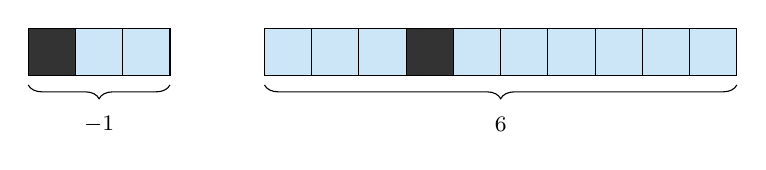
\begin{tikzpicture}[scale=1.2]

\filldraw[fill=black!80!white, draw=black] 
(0,0) rectangle (0.5, 0.5);

\filldraw[fill=cyan!80!blue!20!white, draw=black] 
(0.5,0) rectangle (1, 0.5);

\filldraw[fill=cyan!80!blue!20!white, draw=black] 
(1,0) rectangle (1.5, 0.5);

\filldraw[fill=cyan!80!blue!20!white, draw=black] 
(2.5,0) rectangle (3, 0.5);

\filldraw[fill=cyan!80!blue!20!white, draw=black] 
(3,0) rectangle (3.5, 0.5);

\filldraw[fill=cyan!80!blue!20!white, draw=black] 
(3.5,0) rectangle (4, 0.5);

\filldraw[fill=black!80!white, draw=black] 
(4,0) rectangle (4.5, 0.5);

\filldraw[fill=cyan!80!blue!20!white, draw=black] 
(4.5,0) rectangle (5, 0.5);

\filldraw[fill=cyan!80!blue!20!white, draw=black] 
(5,0) rectangle (5.5, 0.5);

\filldraw[fill=cyan!80!blue!20!white, draw=black] 
(5.5,0) rectangle (6, 0.5);

\filldraw[fill=cyan!80!blue!20!white, draw=black] 
(6,0) rectangle (6.5, 0.5);

\filldraw[fill=cyan!80!blue!20!white, draw=black] 
(6.5,0) rectangle (7, 0.5);

\filldraw[fill=cyan!80!blue!20!white, draw=black] 
(7,0) rectangle (7.5, 0.5);

\draw [decorate,decoration={brace,mirror,amplitude=5pt}]
    (0,-0.1) -- (1.5,-0.1) node [midway,yshift=-0.5cm] {\footnotesize{$-1$}};

\draw [decorate,decoration={brace,mirror,amplitude=5pt}]
    (2.5,-0.1) -- (7.5,-0.1) node [midway,yshift=-0.5cm] {\footnotesize{$6$}};

\end{tikzpicture}}
\caption[Example of an output vector]{Example of an output vector. This particular set of vectors would refer to an output representing a six step downward pitch moment, where the ``$-1$'' label represents the direction of the movement and where the ``$6$'' label represents the number of step in that direction.}
\label{fig:output-vector}
\end{figure}







